\documentclass[10pt,openany]{book}
 
\usepackage{geometry, graphicx, floatflt, varioref, soul, verbatim, amsmath, calc, caption, wasysym, footmisc, makeidx, ifthen, subfigure, multicol, epstopdf, enumerate, wrapfig, textcomp, multirow, changepage, setspace, lscape, titlesec}
%\usepackage[numbers]{natbib}
\usepackage[usenames,dvipsnames]{color}  
%\newcommand{\href}[2]{#2} \newcommand{\url}[1]{#1} \newcommand{\urlstyle}[1]{}
\include{extraTeX/style/colorsV1}
\usepackage[bookmarksnumbered, colorlinks=false,pdfborder={0 0 0},urlcolor= oiGB,colorlinks=true,linkcolor= oiGB, citecolor= oiGB,backref=true]{hyperref}
%\usepackage[colorlinks=false,pdfborder={0 0 0},urlcolor= black,colorlinks=black,linkcolor=black, citecolor=black,backref=true]{hyperref}
\usepackage[style=authortitle-ibid, maxnames=2,natbib=true,sortcites=true,block=space,backend=bibtex]{biblatex}
\bibliography{eoce}
%\usepackage{ifsym}
%\usepackage{fancybox}

\makeindex
\include{extraTeX/style/styleV5}
\include{extraTeX/style/tablet}
\include{extraTeX/preamble/title}
\date{}
\setcounter{tocdepth}{1}

\begin{document}
\renewcommand{\thepage}{}
\maketitle
\include{extraTeX/preamble/copyright}
\renewcommand{\thepage}{\roman{page}}
\tableofcontents
\include{extraTeX/preamble/preface}

\setcounter{page}{1}
\renewcommand{\thepage}{\arabic{page}}

% Chapter 1: Introduction to data
\normalsize\chapter{Introduction to data}
\label{introductionToData}

%\begin{tipBox}{\tipBoxTitle[Chapter Goal:]{Thinking about data}
%Understand basics about data organization, data types, numerical summaries of data, graphical summaries of data, and foundational techniques for data collection. We begin and end the chapter with case studies.}
%\end{tipBox}

Scientists seek to answer questions using rigorous methods and careful observations. These observations -- collected from the likes of field notes, surveys, and experiments -- form the backbone of a statistical investigation and are called \term{data}. Statistics is the study of how best to collect, analyze, and draw conclusions from data. It is helpful to put statistics in the context of a general process of investigation:
\begin{enumerate}
\setlength{\itemsep}{0mm}
\item Identify a question or problem.
\item Collect relevant data on the topic.
\item Analyze the data.
\item Form a conclusion.
%\item Make decisions based on the conclusion.
\end{enumerate}
Statistics as a subject focuses on making stages 2-4 objective, rigorous, and efficient. That~is, statistics has three primary components: How best can we collect data? How should it be analyzed? And what can we infer from the analysis?

The topics scientists investigate are as diverse as the questions they ask. However, many of these investigations can be addressed with a small number of data collection techniques, analytic tools, and fundamental concepts in statistical inference. This chapter provides a glimpse into these and other themes we will encounter throughout the rest of the book. We introduce the basic principles of each branch and learn some tools along the way. We will encounter applications from other fields, some of which are not typically associated with science but nonetheless can benefit from statistical study.

\section[Case study]{Case study: using stents to prevent strokes}
\label{basicExampleOfStentsAndStrokes}

\index{data!stroke|(}

Section~\ref{basicExampleOfStentsAndStrokes} introduces a classic challenge in statistics: evaluating the efficacy of a medical treatment. Terms in this section, and indeed much of this chapter, will all be revisited later in the text. The plan for now is simply to get a sense of the role statistics can play in practice.

In this section we will consider an experiment that studies effectiveness of stents in treating patients at risk of stroke.\footnote{Chimowitz MI, Lynn MJ, Derdeyn CP, et al. 2011. Stenting versus Aggressive Medical Therapy for Intracranial Arterial Stenosis. New England Journal of Medicine 365:993-1003. \urlwofont{http://www.nejm.org/doi/full/10.1056/NEJMoa1105335}. NY Times article reporting on the study: \urlwofont{http://www.nytimes.com/2011/09/08/health/research/08stent.html}.} Stents are small mesh tubes that are placed inside narrow or weak arteries to assist in patient recovery after cardiac events and reduce the risk of an additional heart attack or death. Many doctors have hoped that there would be similar benefits for patients at risk of stroke. We start by writing the principal question the researchers hope to answer:
\begin{quote}
Does the use of stents reduce the risk of stroke?
\end{quote}

The researchers who asked this question collected data on 451 at-risk patients. Each volunteer patient was randomly assigned to one of two groups:
\begin{itemize}
\item[]\termsub{Treatment group}{treatment group}. Patients in the treatment group received a stent and medical management. The medical management included medications, management of risk factors, and help in lifestyle modification.
\item[]\termsub{Control group}{control group}. Patients in the control group received the same medical management as the treatment group but did not receive stents.
\end{itemize}
Researchers randomly assigned 224 patients to the treatment group and 227 to the control group. In this study, the control group provides a reference point against which we can measure the medical impact of stents in the treatment group.

Researchers studied the effect of stents at two time points: 30~days after enrollment and 365~days after enrollment. The results of 5 patients are summarized in Table~\ref{stentStudyResultsDF}. Patient outcomes are recorded as ``stroke'' or ``no event''.

\begin{table}[h]
\centering
\begin{tabular}{l ccc}
\hline
Patient	&	group	&	0-30 days 	&	0-365 days \\
\hline
1		&	treatment &	no event &	no event \\
2		&	treatment &	stroke & stroke \\
3		&	treatment &	no event & no event \\
$\vdots$	&	$\vdots$	  &	$\vdots$ \\
450	&	control &	no event &	no event \\
451	&	control &	no event &	no event \\
\hline
\end{tabular}
\caption{Results for five patients from the stent study.}
\label{stentStudyResultsDF}
% trmt <- c(rep('trmt', 224), rep('control', 227)); outcome30 <- c(rep(c('event', 'no_event'), c(33, 191)), rep(c('event', 'no_event'), c(13, 214))); outcome365 <- c(rep(c('event', 'no_event'), c(33, 191)), rep(c('event', 'no_event'), c(13, 214)))
\end{table}

Considering data from each patient individually would be a long, cumbersome path towards answering the original research question. Instead, a statistical analysis allows us to consider all of the data at once. Table~\ref{stentStudyResults} summarizes the raw data in a more helpful way. In this table, we can quickly see what happened over the entire study. For instance, to identify the number of patients in the treatment group who had a stroke within 30 days, we look on the left-side of the table at the intersection of the treatment and stroke: 33.

\begin{table}[h]
\centering
\begin{tabular}{l cc c cc}
& \multicolumn{2}{c}{0-30 days} &\hspace{5mm}\ & \multicolumn{2}{c}{0-365 days} \\
  \cline{2-3} \cline{5-6}
	& 	stroke 	& no event && 	stroke 	& no event \\
  \hline
treatment 	& 33		& 191	&&	45 	& 179 \\
control 		& 13		& 214	&& 	28	& 199 \\
  \hline
Total				& 46		& 405	&&	73	& 378 \\
  \hline
\end{tabular}
\caption{Descriptive statistics for the stent study.}
\label{stentStudyResults}
\end{table}

\textA{\pagebreak}

\begin{exercise}
Of the 224 patients in the treatment group, 45 had a stroke by the end of the first year. Using these two numbers, compute the proportion of patients in the treatment group who had a stroke by the end of their first year. (Answers to all in-text exercises are provided in footnotes.)\footnote{The proportion of the 224 patients who had a stroke within 365 days: $45/224 = 0.20$.}
\end{exercise}

We can compute summary statistics from the table. A \term{summary statistic} is a single number summarizing a large amount of data.\footnote{Formally, a summary statistic is a value computed from the data. Some summary statistics are more useful than others.} For instance, the primary results of the study after 1~year could be described by two summary statistics: the proportion of people who had a stroke in the treatment and control groups.
\begin{itemize}
\setlength{\itemsep}{0mm}
\item[] Proportion who had a stroke in the treatment (stent) group: $45/224 = 0.20 = 20\%$.
\item[] Proportion who had a stroke in the control group: $28/227 = 0.12 = 12\%$.
\end{itemize}
These two summary statistics are useful in looking for differences in the groups, and we are in for a surprise: an additional 8\% of patients in the treatment group had a stroke! This is important for two reasons. First, it is contrary to what doctors expected, which was that stents would \emph{reduce} the rate of strokes. Second, it leads to a statistical question: do the data show a ``real'' difference due to the treatment?

This second question is subtle. Suppose you flip a coin 100 times. While the chance a coin lands heads in any given coin flip is 50\%, we probably won't observe exactly 50 heads. This type of fluctuation is part of almost any type of data generating process. It is possible that the 8\% difference in the stent study is due to this natural variation. However, the larger the difference we observe (for a particular sample size), the less believable it is that the difference is due to chance. So what we are really asking is the following: is the difference so large that we should reject the notion that it was due to chance?

While we haven't yet covered statistical tools to fully address this question, we can comprehend the conclusions of the published analysis: there was compelling evidence of harm by stents in this study of stroke patients.

\textbf{Be careful:} do not generalize the results of this study to all patients and all stents. This study looked at patients with very specific characteristics who volunteered to be a part of this study and who may not be representative of all stroke patients. In addition, there are many types of stents and this study only considered the self-expanding Wingspan stent (Boston Scientific). However, this study does leave us with an important lesson: we should keep our eyes open for surprises.

\index{data!stroke|)}

\section{Taxonomy of data} %old title: Data basics
\label{dataBasics}

Effective presentation and description of data is a first step in most analyses. This section introduces one structure for organizing data as well as some terminology that will be used throughout this book.

\subsection{Observations, variables, and data matrices}

\index{data!email50|(}

Table~\ref{email50DF} displays rows 1, 2, 3, and 50 of a data set concerning 50 emails received in 2012. These observations will be referred to as the \data{email50} data set, and they are a random sample from a larger data set that we will see in Section~\ref{categoricalData}.

Each row in the table represents a single email or \term{case}.\footnote{A case is also sometimes called a \term{unit of observation} or an \term{observational unit}.} The columns represent characteristics, called \termsub{variables}{variable}, for each of the emails. For example, the first row represents email 1, which is not spam, contains 21,705 characters, 551 line breaks, is written in HTML format, and contains only small numbers.

In practice, it is especially important to ask clarifying questions to ensure important aspects of the data are understood. For instance, it is always important to be sure we know what each variable means and the units of measurement. Descriptions of all five email variables are given in Table~\ref{email50Variables}.

\begin{table}[t]
\centering
\begin{tabular}{cc ccc c}
  \hline
 & \var{spam} & \var{num\_\hspace{0.3mm}char} & \var{line\_\hspace{0.3mm}breaks} & \var{format} & \var{number} \\ 
  \hline
1 & no & 21,705 & 551 & html & small \\ 
  2 & no & 7,011 & 183 & html & big \\ 
  3 & yes & 631 & 28 & text & none \\ 
$\vdots$ & $\vdots$ & $\vdots$ & $\vdots$ & $\vdots$ & $\vdots$ \\
  50 & no & 15,829 & 242 & html & small \\ 
   \hline
\end{tabular}
\caption{Four rows from the \data{email50} data matrix.}
\label{email50DF}
\end{table}
% library(openintro); library(xtable); data(email50); email50[c(1,2,3,50),c("spam", "num_char", "line_breaks", "format", "number")]; xtable(email50[c(1,2,3,50),c("spam", "num_char", "line_breaks", "format", "number")], digits=0)


\begin{table}[t]
\centering\small
\begin{tabular}{lp{10.5cm}}
\hline
{\bf variable} & {\bf description} \\
\hline
\var{spam} & Specifies whether the message was spam \\
\var{num\_\hspace{0.3mm}char} & The number of characters in the email   \\
\var{line\_\hspace{0.3mm}breaks} & The number of line breaks in the email (not including text wrapping)   \\
\var{format} & Indicates if the email contained special formatting, such as bolding, tables, or links, which would indicate the message is in HTML format    \\
\var{number} & Indicates whether the email contained no number, a small number (under 1 million), or a large number   \\
\hline
\end{tabular}
\caption{Variables and their descriptions for the \data{email50} data set.\vspaceA{-3.5mm}}
\label{email50Variables}
\end{table}

\index{data!email50|)}

The data in Table~\ref{email50DF} represent a \term{data matrix}, which is a common way to organize data. Each row of a data matrix corresponds to a unique case, and each column corresponds to a variable. A data matrix for the stroke study introduced in Section~\ref{basicExampleOfStentsAndStrokes} is shown in Table~\vref{stentStudyResultsDF}, where the cases were patients and there were three variables recorded for each patient.

Data matrices are a convenient way to record and store data. If another individual or case is added to the data set, an additional row can be easily added. Similarly, another column can be added for a new variable.

\index{data!county|(}

\begin{exercise}
We consider a publicly available data set that summarizes information about the 3,143 counties in the United States, and we call this the \data{county} data set. This data set includes information about each county: its name, the state where it resides, its population in 2000 and 2010, per capita federal spending, poverty rate, and five additional characteristics. How might these data be organized in a data matrix? Reminder: look in the footnotes for answers to in-text exercises.\footnote{Each county may be viewed as a case, and there are eleven pieces of information recorded for each case. A table with 3,143 rows and 11 columns could hold these data, where each row represents a county and each column represents a particular piece of information.}
\end{exercise}

\noindent Seven rows of the \data{county} data set are shown in Table~\ref{countyDF}, and the variables are summarized in Table~\ref{countyVariables}. These data were collected from the US Census website.\footnote{\urlwofont{http://quickfacts.census.gov/qfd/index.html}}

\begin{landscape}
\begin{table}
\centering\small
\begin{tabular}{ccc ccc ccc ccc}
\hline
& \var{name} & \var{state} & \var{pop2000} & \var{pop2010} &
   \var{fed\_\hspace{0.3mm}spend} & \var{poverty} & \var{homeownership} & \var{multiunit} &
   \var{income} & \var{med\_\hspace{0.3mm}income} & \var{smoking\_\hspace{0.3mm}ban} \\
\hline
  1 & Autauga & AL & 43671 & 54571 & 6.068 & 10.6 & 77.5 & 7.2 & 24568 & 53255 & none \\
  2 & Baldwin & AL & 140415 & 182265 & 6.140 & 12.2 & 76.7 & 22.6 & 26469 & 50147 & none \\ 
  3 & Barbour & AL & 29038 & 27457 & 8.752 & 25.0 & 68.0 & 11.1 & 15875 & 33219 & none \\ 
  4 & Bibb & AL & 20826 & 22915 & 7.122 & 12.6 & 82.9 & 6.6 & 19918 & 41770 & none \\ 
  5 & Blount & AL & 51024 & 57322 & 5.131 & 13.4 & 82.0 & 3.7 & 21070 & 45549 & none \\ 
  $\vdots$ & $\vdots$ & $\vdots$ & $\vdots$ & $\vdots$ & $\vdots$ & $\vdots$ & $\vdots$ & $\vdots$ & $\vdots$ & $\vdots$ & $\vdots$ \\
  3142 & Washakie & WY & 8289 & 8533 & 8.714 & 5.6 & 70.9 & 10.0 & 28557 & 48379 & none \\ 
  3143 & Weston & WY & 6644 & 7208 & 6.695 & 7.9 & 77.9 & 6.5 & 28463 & 53853 & none \\ 
\hline
\end{tabular}
\caption{Seven rows from the \data{county} data set.}
\label{countyDF}
% library(openintro); county <- countyComplete[,c("name", "state", "pop2000", "pop2010", "fed_spending", "poverty", "home_ownership", "housing_multi_unit", "per_capita_income", "median_household_income")]; colnames(county) <- c("name", "state", "pop2000", "pop2010", "fed_spend", "poverty", "homeownership", "multiunit", "income", "med_income"); county$fed_spend <- county$fed_spend / county$pop2010

% library(openintro); library(xtable); cc <- countyComplete; xtable(cc[c(1:5,nrow(cc) - (1:0)), c("name", "state", "pop2000", "pop2010", "fed_spend", "poverty", "homeownership", "multiunit", "income", "med_income")], digits=1)
\end{table}

\begin{table}
\centering\small
\begin{tabular}{lp{11cm}}
\hline
{\bf variable} & {\bf description} \\
\hline
\var{name} & County name \\
\var{state} & State where the county resides (also including the District of Columbia) \\
\var{pop2000} & Population in 2000 \\
\var{pop2010} & Population in 2010 \\
\var{fed\_\hspace{0.3mm}spend} & Federal spending per capita \\
\var{poverty}  &  Percent of the population in poverty \\
\var{homeownership}  &  Percent of the population that lives in their own home or lives with the owner (e.g. children living with parents who own the home) \\
\var{multiunit}  &  Percent of living units that are in multi-unit structures (e.g. apartments) \\
\var{income} & Income per capita \\
\var{med\_\hspace{0.3mm}income} & Median household income for the county, where a household's income equals the total income of its occupants who are 15 years or older \\
\var{smoking\_\hspace{0.3mm}ban}  &  Type of county-wide smoking ban in place at the end of 2011, which takes
			one of three values: \resp{none}, \resp{partial}, or \resp{comprehensive},
			where a \resp{comprehensive} ban means smoking
			was not permitted in restaurants, bars, or workplaces, and \resp{partial}
			means smoking was banned in at least one of those three locations \\
\hline
\end{tabular}
\centering
\caption{Variables and their descriptions for the \data{county} data set.}
\label{countyVariables}
\end{table}
\end{landscape}

\subsection{Types of variables}
\label{variableTypes}

Examine the \var{fed\_\hspace{0.3mm}spend}, \var{pop2010}, \var{state}, and \var{smoking\_\hspace{0.3mm}ban} variables in the \data{county} data set. Each of these variables is inherently different from the other three yet many of them share certain characteristics.

First consider \var{fed\_\hspace{0.3mm}spend}, which is said to be a \term{numerical} variable since it can take a wide range of numerical values, and it is sensible to add, subtract, or take averages with those values. On the other hand, we would not classify a variable reporting telephone area codes as numerical since their average, sum, and difference have no clear meaning.

The \var{pop2010} variable is also numerical, although it seems to be a little different than \var{fed\_\hspace{0.3mm}spend}. This variable of the population count can only be a whole non-negative number (\resp{0}, \resp{1}, \resp{2}, ...). For this reason, the population variable is said to be \term{discrete} since it can only take numerical values with jumps. On the other hand, the federal spending variable is said to be \term{continuous}.

The variable \var{state} can take up to 51 values after accounting for Washington, DC: \resp{AL}, ..., and \resp{WY}. Because the responses themselves are categories, \var{state} is called a \term{categorical} variable,\footnote{Sometimes also called a \term{nominal} variable.} and the possible values are called the variable's \term{levels}.

\begin{figure}
\centering
\includegraphics[width=0.57\textwidth]{01/figures/variables/variables}
\caption{Breakdown of variables into their respective types.}
\label{variables}
\end{figure}

Finally, consider the \var{smoking\_\hspace{0.3mm}ban} variable, which describes the type of county-wide smoking ban and takes a value \resp{none}, \resp{partial}, or \resp{comprehensive} in each county. This variable seems to be a hybrid: it is a categorical variable but the levels have a natural ordering. A variable with these properties is called an \term{ordinal} variable. To simplify analyses, any ordinal variables in this book will be treated as categorical variables.

\begin{example}{Data were collected about students in a statistics course. Three variables were recorded for each student: number of siblings, student height, and whether the student had previously taken a statistics course. Classify each of the variables as continuous numerical, discrete numerical, or categorical.}
The number of siblings and student height represent numerical variables. Because the number of siblings is a count, it is discrete. Height varies continuously, so it is a continuous numerical variable. The last variable classifies students into two categories -- those who have and those who have not taken a statistics course -- which makes this variable categorical.
\end{example}

\begin{exercise} \index{data!stroke}
Consider the variables \var{group} and \var{outcome} (at 30 days) from the stent study in Section~\ref{basicExampleOfStentsAndStrokes}. Are these numerical or categorical variables?\footnote{There are only two possible values for each variable, and in both cases they describe categories. Thus, each is a categorical variable.}
\end{exercise}

\subsection{Relationships between variables}
\label{variableRelations}

Many analyses are motivated by a researcher looking for a relationship between two or more variables. A social scientist may like to answer some of the following questions:
\begin{enumerate}
\setlength{\itemsep}{0mm}
\item[(1)]\label{fedSpendingPovertyQuestion} Is federal spending, on average, higher or lower in counties with high rates of poverty?
\item[(2)]\label{ownershipMultiUnitQuestion} If homeownership is lower than the national average in one county, will the percent of multi-unit structures in that county likely be above or below the national average?
\item[(3)]\label{isAverageIncomeAssociatedWithSmokingBans} Which counties have a higher average income: those that enact one or more smoking bans or those that do not?
\end{enumerate}

To answer these questions, data must be collected, such as the \data{county} data set shown in Table~\ref{countyDF}. Examining summary statistics \index{summary statistic} could provide insights for each of the three questions about counties. Additionally, graphs can be used to visually summarize data and are useful for answering such questions as well.

\indexthis{Scatterplots}{scatterplot} are one type of graph used to study the relationship between two numerical variables. Figure~\ref{county_fed_spendVsPoverty} compares the variables \var{fed\_\hspace{0.3mm}spend} and \var{poverty}. Each point on the plot represents a single county. For instance, the highlighted dot corresponds to County~1088 in the \data{county} data set: Owsley County, Kentucky, which had a poverty rate of 41.5\% and federal spending of \$21.50 per capita. The dense cloud in the scatterplot suggests a relationship between the two variables: counties with a high poverty rate also tend to have slightly more federal spending. We might brainstorm as to why this relationship exists and investigate each idea to determine which is the most reasonable explanation.

\begin{figure}
\centering
\includegraphics[width=0.8\textwidth]{01/figures/county_fed_spendVsPoverty/county_fed_spendVsPoverty}
\caption{A scatterplot showing \var{fed\_\hspace{0.3mm}spend} against \var{poverty}. Owsley County of Kentucky, with a poverty rate of 41.5\% and federal spending of \$21.50 per capita, is highlighted.}
\label{county_fed_spendVsPoverty}
\end{figure}

\begin{exercise}
Examine the variables in the \data{email50} data set, which are described in Table~\vref{email50Variables}. Create two questions about the relationships between these variables that are of interest to you.\footnote{Two sample questions: (1) Intuition suggests that if there are many line breaks in an email then there would also tend to be many characters: does this hold true? (2)~Is there a connection between whether an email format is plain text (versus HTML) and whether it is a spam message?}
\end{exercise}

The \var{fed\_\hspace{0.3mm}spend} and \var{poverty} variables are said to be associated because the plot shows a discernible pattern. When two variables show some connection with one another, they are called \term{associated} variables. Associated variables can also be called \term{dependent} variables and vice-versa.

\begin{example}{ The relationship between the homeownership rate and the percent of units in multi-unit structures (e.g. apartments, condos) is visualized using a scatterplot in Figure~\ref{multiunitsVsOwnership}. Are these variables associated?}
It appears that the larger the fraction of units in multi-unit structures, the lower the homeownership rate. Since there is some relationship between the variables, they are associated.
\end{example}


\begin{figure}
   \centering
   \includegraphics[width=0.8\textwidth]{01/figures/multiunitsVsOwnership/multiunitsVsOwnership}
   \caption{A scatterplot of the homeownership rate versus the percent of units that are in multi-unit structures for all 3,143 counties. Interested readers may find an image of this plot with an additional third variable, county population, presented at \href{http://www.openintro.org/stat/down/MHP.png}{www.openintro.org/stat/down/MHP.png}.}
   \label{multiunitsVsOwnership}
\end{figure}

Because there is a downward trend in Figure~\ref{multiunitsVsOwnership} -- counties with more units in multi-unit structures are associated with lower homeownership -- these variables are said to be \termsub{negatively associated}{negative association}. A \term{positive association} is shown in the relationship between the \var{poverty} and \var{fed\_\hspace{0.3mm}spend} variables represented in Figure~\ref{county_fed_spendVsPoverty}, where counties with higher poverty rates tend to receive more federal spending per capita.

If two variables are not associated, then they are said to be \term{independent}. That is, two variables are independent if there is no evident relationship between the two.

\begin{termBox}{\tBoxTitle{Associated or independent, not both}
A pair of variables are either related in some way (associated) or not (independent). No pair of variables is both associated and independent.}
\end{termBox}

\index{data!county|)}

%%%%%
\section{Overview of data collection principles}
\label{overviewOfDataCollectionPrinciples}

\index{sample|(}
\index{population|(}

The first step in conducting research is to identify topics or questions that are to be investigated. A clearly laid out research question is helpful in identifying what subjects or cases should be studied and what variables are important. It is also important to consider \emph{how} data are collected so that they are reliable and help achieve the research goals.

\subsection{Populations and samples}
\label{populationsAndSamples}

Consider the following three research questions:
\begin{enumerate}
\setlength{\itemsep}{0mm}
\item What is the average mercury content in swordfish in the Atlantic Ocean?
\item\label{timeToGraduationQuestionForUCLAStudents} Over the last 5 years, what is the average time to complete a degree for Duke undergraduate students?
\item\label{identifyPopulationOfStentStudy} Does a new drug reduce the number of deaths in patients with severe heart disease?
\end{enumerate}
Each research question refers to a target \term{population}. In the first question, the target population is all swordfish in the Atlantic ocean, and each fish represents a case. It is usually too expensive to collect data for every case in a population. Instead, a sample is taken. A \term{sample} represents a subset of the cases and is often a small fraction of the population. For instance, 60 swordfish (or some other number) in the population might be selected, and this sample data may be used to provide an estimate of the population average and answer the research question.

\begin{exercise} \label{identifyingThePopulationForTwoQuestionsInPopAndSampSubsection}
For the second and third questions above, identify the target population and what represents an individual case.\footnote{(\ref{timeToGraduationQuestionForUCLAStudents}) Notice that the first question is only relevant to students who complete their degree; the average cannot be computed using a student who never finished her degree. Thus, only Duke undergraduate students who have graduated in the last five years represent cases in the population under consideration. Each such student would represent an individual case. (\ref{identifyPopulationOfStentStudy}) A person with severe heart disease represents a case. The population includes all people with severe heart disease.}
\end{exercise}


\subsection{Anecdotal evidence}
\label{anecdotalEvidenceSubsection}

Consider the following possible responses to the three research questions:
\begin{enumerate}
\item A man on the news got mercury poisoning from eating swordfish, so the average mercury concentration in swordfish must be dangerously high.
\item\label{iKnowThreeStudentsWhoTookMoreThan7YearsToGraduateAtDuke} I met two students who took more than 7 years to graduate from Duke, so it must take longer to graduate at Duke than at many other colleges.
\item\label{myFriendsDadDiedAfterSulphinpyrazon} My friend's dad had a heart attack and died after they gave him a new heart disease drug, so the drug must not work.
\end{enumerate}
Each conclusion is based on data. However, there are two problems. First, the data only represent one or two cases. Second, and more importantly, it is unclear whether these cases are actually representative of the population. Data collected in this haphazard fashion are called \term{anecdotal evidence}.

\setlength{\captionwidth}{\textwidth-80mm}
\begin{figure}
\centering
\hspace{8mm}\includegraphics[width=55mm]{01/figures/mnWinter/mnWinter}\hspace{4mm}
\begin{minipage}[b]{\textwidth - 80mm}
   \caption[anecdotal evidence]{In February 2010, some media pundits cited one large snow storm as evidence against global warming. As comedian Jon Stewart pointed out, ``It's one storm, in one region, of one country.''\vspace{-4.5mm} \\
   
   -----------------------------\vspace{-2mm}\\
   {\footnotesize February 10th, 2010.}
   \label{mnWinter}}
\end{minipage}
\end{figure}
\setlength{\captionwidth}{\mycaptionwidth}

\begin{termBox}{\tBoxTitle{Anecdotal evidence}
Be careful of data collected haphazardly. Such evidence may be true and verifiable, but it may only represent extraordinary cases.}
\end{termBox}

Anecdotal evidence typically is composed of unusual cases that we recall based on their striking characteristics. For instance, we are more likely to remember the two people we met who took 7 years to graduate than the six others who graduated in four years. Instead of looking at the most unusual cases, we should examine a sample of many cases that represent the population.

\subsection{Sampling from a population}

\index{sample!random sample|(}

We might try to estimate the time to graduation for Duke undergraduates in the last 5 years by collecting a sample of students. All graduates in the last 5 years represent the \emph{population}\index{population}, and graduates who are selected for review are collectively called the \emph{sample}\index{sample}. In general, we always seek to \emph{randomly} select a sample from a population. The most basic type of random selection is equivalent to how raffles are conducted. For example, in selecting graduates, we could write each graduate's name on a raffle ticket and draw 100 tickets. The selected names would represent a random sample of 100 graduates.

\begin{figure}[ht]
\centering
\includegraphics[width=0.47\textwidth]{01/figures/popToSample/popToSampleGraduates}
\caption{In this graphic, five graduates are randomly selected from the population to be included in the sample.}
\label{popToSampleGraduates}
\end{figure}

Why pick a sample randomly? Why not just pick a sample by hand? Consider the following scenario.

\begin{example}{Suppose we ask a student who happens to be majoring in nutrition to select several graduates for the study. What kind of students do you think she might collect? Do you think her sample would be representative of all graduates?}
Perhaps she would pick a disproportionate number of graduates from health-related fields. Or perhaps her selection would be well-representative of the population. When selecting samples by hand, we run the risk of picking a \emph{biased} sample, even if that bias is unintentional or difficult to discern.
\end{example}

\begin{figure}
\centering
\includegraphics[width=0.47\textwidth]{01/figures/popToSample/popToSubSampleGraduates}
\caption{Instead of sampling from all graduates equally, a nutrition major might inadvertently pick graduates with health-related majors disproportionately often.}
\label{popToSubSampleGraduates}
\end{figure}

If someone was permitted to pick and choose exactly which graduates were included in the sample, it is entirely possible that the sample could be skewed to that person's interests, which may be entirely unintentional. This introduces \term{bias} into a sample. Sampling randomly helps resolve this problem. The most basic random sample is called a \term{simple random sample}, which is equivalent to using a raffle to select cases. This means that each case in the population has an equal chance of being included and there is no implied connection between the cases in the sample.

\APVersion{Sometimes a simple random sample is difficult to implement and an alternative method is helpful. One such substitute is a \term{systematic sample}, where one case is sampled after letting a fixed number of others, say 10 other cases, pass by. Since this approach uses a mechanism that is not easily subject to personal biases, it often yields a reasonably representative sample. This book will focus on random samples since the use of systematic samples is uncommon and requires additional considerations of the context.}{}

The act of taking a simple random sample helps minimize bias, however, bias can crop up in other ways.
Even when people are picked at random, e.g. for surveys, caution must be exercised if the \term{non-response} \index{sample!non-response|textbf} is high. For instance, if only 30\% of the people randomly sampled for a survey actually respond, and it is unclear whether the respondents are \term{representative} of the entire population, the survey might suffer from \term{non-response~bias}.\index{sample!non-response bias|textbf}

\begin{figure}[h]
\centering
\includegraphics[width=0.5\textwidth]{01/figures/popToSample/surveySample}
\caption{Due to the possibility of non-response, surveys studies may only reach a certain group within the population. It is difficult, and often impossible, to completely fix this problem.}
\label{surveySample}
\end{figure}

Another common downfall is a \term{convenience sample}\index{sample!convenience sample}, where individuals who are easily accessible are more likely to be included in the sample. For instance, if a political survey is done by stopping people walking in the Bronx, it will not represent all of New York City. It is often difficult to discern what sub-population a convenience sample represents.

\begin{exercise}
We can easily access ratings for products, sellers, and companies through websites. These ratings are based only on those people who go out of their way to provide a rating. If 50\% of online reviews for a product are negative, do you think this means that 50\% of buyers are dissatisfied with the product?\footnote{Answers will vary. From our own anecdotal experiences, we believe people tend to rant more about products that fell below expectations than rave about those that perform as expected. For this reason, we suspect there is a negative bias in product ratings on sites like Amazon. However, since our experiences may not be representative, we also keep an open mind.}
\end{exercise}

\index{sample!random sample|)}
\index{population|)}
\index{sample|)}

\subsection{Explanatory and response variables}
\label{explanatoryAndResponse}

\index{data!county|(}

Consider the following question from page~\pageref{fedSpendingPovertyQuestion} for the \data{county} data set:
\begin{enumerate}
\item[(1)] 
	Is federal spending, on average, higher or lower in counties with high rates of poverty?
\end{enumerate}
If we suspect poverty might affect spending in a county, then poverty is the \term{explanatory} variable and federal spending is the \term{response} variable in the relationship.\footnote{Sometimes the explanatory variable is called the \term{independent} variable and the response variable is called the \term{dependent} variable. However, this becomes confusing since a \emph{pair} of variables might be independent or dependent, so we avoid this language.} If there are many variables, it may be possible to consider a number of them as explanatory variables.

\begin{tipBox}{\tipBoxTitle{Explanatory and response variables}
To identify the explanatory variable in a pair of variables, identify which of the two is suspected of affecting the other.

\hspace{10mm}\includegraphics[height=0.34in]{01/figures/expResp/expResp}}
\end{tipBox}

\begin{caution}{association does not imply causation}{Labeling variables as \emph{explanatory} and \emph{response} does not guarantee the relationship between the two is actually causal, even if there is an association identified between the two variables. We use these labels only to keep track of which variable we suspect affects the other.}
\end{caution}

In some cases, there is no explanatory or response variable. Consider the following question from page~\pageref{ownershipMultiUnitQuestion}:
\begin{enumerate}
\item[(2)] 
	If homeownership is lower than the national average in one county, will the percent of multi-unit structures in that county likely be above or below the national average?
\end{enumerate}
It is difficult to decide which of these variables should be considered the explanatory and response variable, i.e. the direction is ambiguous, so no explanatory or response labels are suggested here.

\index{data!county|)}

\subsection{Introducing observational studies and experiments}

There are two primary types of data collection: observational studies and experiments.

Researchers perform an \term{observational study} when they collect data in a way that does not directly interfere with how the data arise. For instance, researchers may collect information via surveys, review medical or company records, or follow a \term{cohort} of many similar individuals to study why certain diseases might develop. In each of these situations, researchers merely observe what happens. In general, observational studies can provide evidence of a naturally occurring association between variables, but they cannot by themselves show a causal connection.

When researchers want to investigate the possibility of a causal connection, they conduct an \term{experiment}. Usually there will be both an explanatory and a response variable. For instance, we may suspect administering a drug will reduce mortality in heart attack patients over the following year. To check if there really is a causal connection between the explanatory variable and the response, researchers will collect a sample of individuals and split them into groups. The individuals in each group are \emph{assigned} a treatment. When individuals are randomly assigned to a group, the experiment is called a \term{randomized experiment}. For example, each heart attack patient in the drug trial could be randomly assigned,  perhaps by flipping a coin, into one of two groups: the first group receives a \term{placebo} (fake treatment) and the second group receives the drug. See the case study in Section~\ref{basicExampleOfStentsAndStrokes} for another example of an experiment, though that study did not employ a placebo.

\begin{tipBox}{\tipBoxTitle{association $\neq$ causation}
In a data analysis, association does not imply causation, and causation can only be inferred from a randomized experiment.}
\end{tipBox}


%%%%%
\section{Observational studies and sampling strategies}

\subsection{Observational studies}

Generally, data in observational studies are collected only by monitoring what occurs, while experiments require the primary explanatory variable in a study be assigned for each subject by the researchers.

Making causal conclusions based on experiments is often reasonable. However, making the same causal conclusions based on observational data can be treacherous and is not recommended. Thus, observational studies are generally only sufficient to show associations.

\begin{exercise} \label{sunscreenLurkingExample}
Suppose an observational study tracked sunscreen use and skin cancer, and it was found that the more sunscreen someone used, the more likely the person was to have skin cancer. Does this mean sunscreen \emph{causes} skin cancer?\footnote{No. See the paragraph following the exercise for an explanation.}
\end{exercise}

Some previous research tells us that using sunscreen actually reduces skin cancer risk, so maybe there is another variable that can explain this hypothetical association between sunscreen usage and skin cancer. One important piece of information that is absent is sun exposure. If someone is out in the sun all day, she is more likely to use sunscreen \emph{and} more likely to get skin cancer. Exposure to the sun is unaccounted for in the simple investigation.
\begin{center}
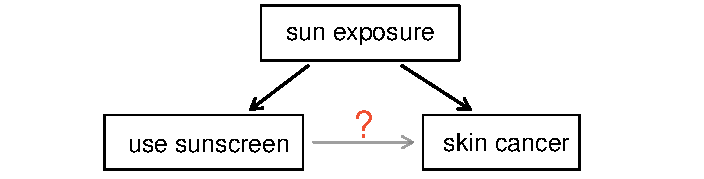
\includegraphics[height=1.0in]{01/figures/variables/sunCausesCancer}
\end{center}
% Some studies:
% http://www.sciencedirect.com/science/article/pii/S0140673698121682
% http://archderm.ama-assn.org/cgi/content/abstract/122/5/537
% Study with a similar scenario to that described here:
% http://onlinelibrary.wiley.com/doi/10.1002/ijc.22745/full

Sun exposure is what is called a \term{confounding variable},\footnote{Also called a \term{lurking variable}, \term{confounding factor}, or a \term{confounder}.} which is a variable that is correlated with both the explanatory and response variables. While one method to justify making causal conclusions from observational studies is to exhaust the search for confounding variables, there is no guarantee that all confounding variables can be examined or measured.

In the same way, the \data{county} data set is an observational study with confounding variables, and its data cannot easily be used to make causal conclusions.

\begin{exercise}
Figure~\ref{multiunitsVsOwnership} shows a negative association between the homeownership rate and the percentage of multi-unit structures in a county. However, it is unreasonable to conclude that there is a causal relationship between the two variables. Suggest one or more other variables that might explain the relationship in Figure~\ref{multiunitsVsOwnership}.~\footnote{Answers will vary. Population density may be important. If a county is very dense, then a larger fraction of residents may live in multi-unit structures. Additionally, the high density may contribute to increases in property value, making homeownership infeasible for many residents.}
\end{exercise}

Observational studies come in two forms: prospective and retrospective studies. A \term{prospective study} identifies individuals and collects information as events unfold. For instance, medical researchers may identify and follow a group of similar individuals over many years to assess the possible influences of behavior on cancer risk. One example of such a study is The Nurses� Health Study, started in 1976 and expanded in 1989.\footnote{\urlwofont{http://www.channing.harvard.edu/nhs/}} This prospective study recruits registered nurses and then collects data from them using questionnaires. \termsub{Retrospective studies}{retrospective studies} collect data after events have taken place, e.g. researchers may review past events in medical records. Some data sets, such as \data{county}, may contain both prospectively- and retrospectively-collected variables. Local governments prospectively collect some variables as events unfolded (e.g. retails sales) while the federal government retrospectively collected others during the 2010 census (e.g. county population).

\subsection{Three sampling methods (special topic)}
\label{threeSamplingMethods}

Almost all statistical methods are based on the notion of implied randomness. If observational data are not collected in a random framework from a population, results from these statistical methods are not reliable. Here we consider three random sampling techniques: simple, stratified, and cluster sampling. Figure~\ref{samplingMethodsFigure} provides a graphical representation of these techniques.

\begin{figure}
\centering
\includegraphics[width=0.8\textwidth]{01/figures/samplingMethodsFigure/samplingMethodsFigure}
\caption{Examples of simple random, stratified, and cluster sampling. In the top panel, simple random sampling was used to randomly select the 18 cases. In the middle panel, stratified sampling was used: cases were grouped into strata, and then simple random sampling was employed within each stratum. In the bottom panel, cluster sampling was used, where data were binned into nine clusters, and three of the clusters were randomly selected.}
\label{samplingMethodsFigure}
\end{figure}

\termsub{Simple random sampling}{sample!simple random sampling} is probably the most intuitive form of random sampling. Consider the salaries of Major League Baseball (MLB) players, where each player is a member of one of the league's 30 teams. To take a simple random sample of 120 baseball players and their salaries from the 2010 season, we could write the names of that season's 828 players onto slips of paper, drop the slips into a bucket, shake the bucket around until we are sure the names are all mixed up, then draw out slips until we have the sample of 120 players. In general, a sample is referred to as ``simple random'' if each case in the population has an equal chance of being included in the final sample \emph{and} knowing that a case is included in a sample does not provide useful information about which other cases are included.

\termsub{Stratified sampling}{sample!stratified sampling} is a divide-and-conquer sampling strategy. The population is divided into groups called \term{strata}\index{sample!strata|textbf}. The strata are chosen so that similar cases are grouped together, then a second sampling method, usually simple random sampling, is employed within each stratum. In the baseball salary example, the teams could represent the strata; some teams have a lot more money (we're looking at you, Yankees). Then we might randomly sample 4 players from each team for a total of 120 players.

Stratified sampling is especially useful when the cases in each stratum are very similar with respect to the outcome of interest. The downside is that analyzing data from a stratified sample is a more complex task than analyzing data from a simple random sample. The analysis methods introduced in this book would need to be extended to analyze data collected using stratified sampling.

\begin{example}{Why would it be good for cases within each stratum to be very similar?}
We might get a more stable estimate for the subpopulation in a stratum if the cases are very similar. These improved estimates for each subpopulation will help us build a reliable estimate for the full population.
\end{example}

In \termsub{cluster sampling}{sample!cluster sample}, we group observations into clusters, then randomly sample some of the clusters. Sometimes cluster sampling can be a more economical technique than the alternatives. Also, unlike stratified sampling, cluster sampling is most helpful when there is a lot of case-to-case variability within a cluster but the clusters themselves don't look very different from one another. For example, if neighborhoods represented clusters, then this sampling method works best when the neighborhoods are very diverse. A downside of cluster sampling is that more advanced analysis techniques are typically required, though the methods in this book can be extended to handle such data.

\begin{example}{Suppose we are interested in estimating the malaria rate in a densely tropical portion of rural Indonesia. We learn that there are 30 villages in that part of the Indonesian jungle, each more or less similar to the next. What sampling method should be employed?}
A simple random sample would likely draw individuals from all 30 villages, which could make data collection extremely expensive. Stratified sampling would be a challenge since it is unclear how we would build strata of similar individuals. However, cluster sampling seems like a very good idea. We might randomly select a small number of villages. This would probably reduce our data collection costs substantially in comparison to a simple random sample and would still give us helpful information.
\end{example}

Another technique called \term{multistage sampling} is similar to cluster sampling, except that we take a simple random sample within each selected cluster. For instance, if we sampled neighborhoods using cluster sampling, we would next sample a subset of homes within each selected neighborhood if we were using multistage sampling.


%%%%%
\section{Experiments}
\label{experimentsSection}

Studies where the researchers assign treatments to cases are called \termsub{experiments}{experiment}. When this assignment includes randomization, e.g.~using a coin flip to decide which treatment a patient receives, it is called a \term{randomized experiment}. Randomized experiments are fundamentally important when trying to show a causal connection between two variables.

\subsection{Principles of experimental design}
\label{experimentalDesignPrinciples}

Randomized experiments are generally built on four principles.
\begin{description}
\item[Controlling.] Researchers assign treatments to cases, and they do their best to \term{control} any other differences in the groups. For example, when patients take a drug in pill form, some patients take the pill with only a sip of water while others may have it with an entire glass of water. To control for the effect of water consumption, a doctor may ask all patients to drink a 12 ounce glass of water with the pill.
\item[Randomization.] Researchers randomize patients into treatment groups to account for variables that cannot be controlled. For example, some patients may be more susceptible to a disease than others due to their dietary habits. Randomizing patients into the treatment or control group helps even out such differences, and it also prevents accidental bias from entering the study.
\item[Replication.] The more cases researchers observe, the more accurately they can estimate the effect of the explanatory variable on the response. In a single study, we \term{replicate} by collecting a sufficiently large sample. Additionally, a group of scientists may replicate an entire study to verify an earlier finding.

\begin{figure}
\centering
\includegraphics[width=0.78\textwidth]{01/figures/figureShowingBlocking/figureShowingBlocking}
\caption{Blocking using a variable depicting patient risk. Patients are first divided into low-risk and high-risk blocks, then each block is evenly divided into the treatment groups using randomization. This strategy ensures an equal representation of patients in each treatment group from both the low-risk and high-risk categories.}
\label{figureShowingBlocking}
\end{figure}

\item[Blocking.] Researchers sometimes know or suspect that variables, other than the treatment, influence the response. Under these circumstances, they may first group individuals based on this variable and then randomize cases within each block to the treatment groups. This strategy is often referred to as \term{blocking}. For instance, if we are looking at the effect of a drug on heart attacks, we might first split patients into low-risk and high-risk \term{blocks}, then randomly assign half the patients from each block to the control group and the other half to the treatment group, as shown in Figure~\ref{figureShowingBlocking}. This strategy ensures each treatment group has an equal number of low-risk and high-risk patients.
\end{description}

It is important to incorporate the first three experimental design principles into any study, and this book describes methods for analyzing data from such experiments. Blocking is a slightly more advanced technique, and statistical methods in this book may be extended to analyze data collected using blocking.

\subsection{Reducing bias in human experiments}
\label{biasInHumanExperiments}

Randomized experiments are the gold standard for data collection, but they do not ensure an unbiased perspective into the cause and effect relationships in all cases. Human studies are perfect examples where bias can unintentionally arise. Here we reconsider a study where a new drug was used to treat heart attack patients.\footnote{Anturane Reinfarction Trial Research Group. 1980. Sulfinpyrazone in the prevention of sudden death after myocardial infarction. New England Journal of Medicine 302(5):250-256.} In particular, researchers wanted to know if the drug reduced deaths in patients.

These researchers designed a randomized experiment because they wanted to draw causal conclusions about the drug's effect. Study volunteers\footnote{Human subjects are often called \term{patients}, \term{volunteers}, or \term{study participants}.} were randomly placed into two study groups. One group, the \term{treatment group}, received the drug. The other group, called the \term{control group}, did not receive any drug treatment.

Put yourself in the place of a person in the study. If you are in the treatment group, you are given a fancy new drug that you anticipate will help you. On the other hand, a person in the other group doesn't receive the drug and sits idly, hoping her participation doesn't increase her risk of death. These perspectives suggest there are actually two effects: the one of interest is the effectiveness of the drug, and the second is an emotional effect that is difficult to quantify.

Researchers aren't usually interested in the emotional effect, which might bias the study. To circumvent this problem, researchers do not want patients to know which group they are in. When researchers keep the patients uninformed about their treatment, the study is said to be \term{blind}. But there is one problem: if a patient doesn't receive a treatment, she will know she is in the control group. The solution to this problem is to give fake treatments to patients in the control group. A fake treatment is called a \term{placebo}, and an effective placebo is the key to making a study truly blind. A classic example of a placebo is a sugar pill that is made to look like the actual treatment pill. Often times, a placebo results in a slight but real improvement in patients. This effect has been dubbed the \term{placebo~effect}.

The patients are not the only ones who should be blinded: doctors and researchers can accidentally bias a study. When a doctor knows a patient has been given the real treatment, she might inadvertently give that patient more attention or care than a patient that she knows is on the placebo. To guard against this bias, which again has been found to have a measurable effect in some instances, most modern studies employ a \term{double-blind} setup where doctors or researchers who interact with patients are, just like the patients, unaware of who is or is not receiving the treatment.\footnote{There are always some researchers in the study who do know which patients are receiving which treatment. However, they do not interact with the study's patients and do not tell the blinded health care professionals who is receiving which treatment.}

\begin{exercise}
Look back to the study in Section~\ref{basicExampleOfStentsAndStrokes} where researchers were testing whether stents were effective at reducing strokes in at-risk patients. Is this an experiment? Was the study blinded? Was it double-blinded?\footnote{The researchers assigned the patients into their treatment groups, so this study was an experiment. However, the patients could distinguish what treatment they received, so this study was not blind. The study could not be double-blind since it was not blind.}
\end{exercise}

%%%%%
\section{Revisit case study}
%\section{Exercises}


%_________________
\subsection{Case study}

% 1

\eoce{\qt{Migraine and acupuncture}
A migraine is a particularly painful type of headache, which patients sometimes wish to treat with acupuncture. To determine whether acupuncture relieves migraine pain, researchers conducted a randomized controlled study where 89 females diagnosed with migraine headaches were randomly assigned to one of two groups: treatment or control. 43 patients in the treatment group received acupuncture that is specifically designed to treat migraines. 46 patients in the control group received placebo acupuncture (needle insertion at nonacupoint locations). 24 hours after patients received acupuncture, they were asked if they were pain free. Results are summarized in the contingency table below. \footfullcite{Allais:2011}

\noindent\begin{minipage}[l]{0.4\textwidth}
\begin{tabular}{ll  cc c} 
			&				& \multicolumn{2}{c}{\textit{Pain free}} \\
\cline{3-4}
			&							& Yes 	& No 	& Total	\\
\cline{2-5}
							&Treatment 	& 10	 	& 33		& 43 	\\
\raisebox{1.5ex}[0pt]{\emph{Group}}	& Control		& 2	 	& 44 	 	& 46 \\
\cline{2-5}
							&Total		& 12		& 77		& 89
\end{tabular}
\end{minipage}
\begin{minipage}[c]{0.05\textwidth}
\end{minipage}
\begin{minipage}[c]{0.27\textwidth}
\begin{center}
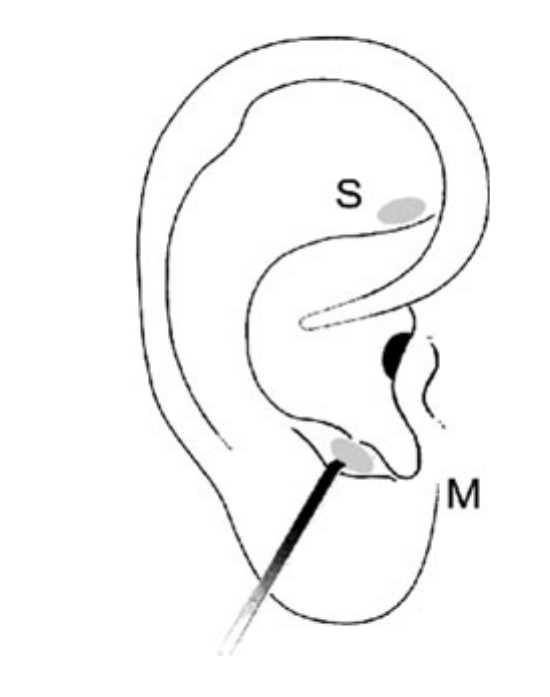
\includegraphics[width = 0.75\textwidth]{01/figures/eoce/images/earacupuncture}
\end{center}
\end{minipage}
\begin{minipage}[c]{0.25\textwidth}
{\footnotesize Figure from the original paper displaying the appropriate area (M) versus the inappropriate area (S) used in the treatment of migraine attacks.}
\end{minipage}
\begin{parts}
\item What percent of patients in the treatment group were pain free 24 hours after receiving acupuncture? What percent in the control group?
\item At first glance, does acupuncture appear to be an effective treatment for migraines? Explain your reasoning.
\item Do the data provide convincing evidence that there is a real pain reduction for those patients in the treatment group? Or do you think that the observed difference might just be due to chance?
\end{parts}
}
{}

% 2

\eoce{\qt{Sinusitis and antibiotics, Part I\label{sinusitis}} Researchers studying the effect of antibiotic treatment for acute sinusitis compared to symptomatic treatments randomly assigned 166 adults diagnosed with acute sinusitis to one of two groups: treatment or control. Study participants received either a 10-day course of amoxicillin (an antibiotic) or a placebo similar in appearance and taste. The placebo consisted of symptomatic treatments such as acetaminophen, nasal decongestants, etc. At the end of the 10-day period patients were asked if they experienced significant improvement in symptoms. The distribution of responses are summarized below. \footfullcite{Garbutt:2012}
\begin{center}
\begin{tabular}{ll  cc c} 
			&				& \multicolumn{2}{c}{\textit{Self-reported significant}} \\
			&				& \multicolumn{2}{c}{\textit{improvement in symptoms}} \\
\cline{3-4}
			&							& Yes 	& No 	& Total	\\
\cline{2-5}
							&Treatment 	& 66	 	& 19		& 85 	\\
\raisebox{1.5ex}[0pt]{\emph{Group}}	& Control		& 65	 	& 16 	 	& 81 \\
\cline{2-5}
							&Total		& 131	& 35		& 166
\end{tabular}
\end{center}
\begin{parts}
\item What percent of patients in the treatment group experienced a significant improvement in symptoms? What percent in the control group?
\item Based on your findings in part (a), which treatment appears to be more effective for sinusitis?
\item Do the data provide convincing evidence that there is a difference in the improvement rates of sinusitis symptoms? Or do you think that the observed difference might just be due to chance?
\end{parts}
}
{}


%_________________
\subsection{Data basics}

% 3

\eoce{\qt{Identify study components, Part I\label{components1}} Identify (i) the cases, (ii) the variables and their types, and (iii) the main research question in the studies described below.
\begin{parts}
\item Researchers collected data to examine the relationship between pollutants and preterm births in Southern California. During the study air pollution levels were measured by air quality monitoring stations. Specifically, levels of carbon monoxide were recorded in parts per million, nitrogen dioxide and ozone in parts per hundred million, and coarse particulate matter (PM$_{10}$) in $\mu g/m^3$. Length of gestation data were collected on 143,196 births between the years 1989 and 1993, and air pollution exposure during gestation was calculated for each birth. The analysis suggested that increased ambient PM$_{10}$ and, to a lesser degree, CO concentrations may be associated with the occurrence of preterm births. \footfullcite{Ritz+Yu+Chapa+Fruin:2000}
\item The Buteyko method is a shallow breathing technique developed by Konstantin Buteyko, a Russian doctor, in 1952. Anecdotal evidence suggests that the Buteyko method can reduce asthma symptoms and improve quality of life. In a scientific study to determine the effectiveness of this method, researchers recruited 600 asthma patients aged 18-69 who relied on medication for asthma treatment. These patients were split into two research groups: one practiced the Buteyko method and the other did not. Patients were scored on quality of life, activity, asthma symptoms, and medication reduction on a scale from 0 to 10. On average, the participants in the Buteyko group experienced a significant reduction in asthma symptoms and an improvement in quality of life. \footfullcite{McDowan:2003}
\end{parts}
}{}

% 4

\eoce{\qt{Identify study components, Part II\label{components2}} Identify (i) the cases, (ii) the variables and their types, and (iii) the main research question of the studies described below.
\begin{parts}
\item While obesity is measured based on body fat percentage (more than 35\% body fat for women and more than 25\% for men), precisely measuring body fat percentage is difficult. Body mass index (BMI), calculated as the ratio $weight/height^2$, is often used as an alternative indicator for obesity. A common criticism of BMI is that it assumes the same relative body fat percentage regardless of age, sex, or ethnicity. In order to determine how useful BMI is for predicting body fat percentage across age, sex and ethnic groups, researchers studied 202 black and 504 white adults who resided in or near New York City, were ages 20-94 years old, had BMIs of 18-35 kg/m$^2$, and who volunteered to be a part of the study. Participants reported their age, sex, and ethnicity and were measured for weight and height. Body fat percentage was measured by submerging the participants in water. \footfullcite{Gallagher:1996} \label{BMIAgeSexEth}

\item In a study of the relationship between socio-economic class and unethical behavior, 129 University of California undergraduates at Berkeley were asked to identify themselves as having low or high social-class by comparing themselves to others with the most (least) money, most (least) education, and most (least) respected jobs. They were also presented  with a jar of individually wrapped candies and informed that they were for children in a nearby laboratory, but that they could take some if they wanted. Participants completed unrelated tasks and then reported the number of candies they had taken. It was found that those in the upper-class rank condition took more candy than did those in the lower-rank condition. \footfullcite{Piff:2012}
\end{parts}
}{}

% 5
\textA{\pagebreak}

\eoce{\qt{Fisher's irises} Sir Ronald Aylmer Fisher was an English statistician, evolutionary biologist, and geneticist who worked on a data set that contained sepal length and width, and petal length and width from three species of iris flowers (\textit{setosa}, \textit{versicolor} and \textit{virginica}). There were 50 flowers from each species in the data set. \footfullcite{Fisher:1936,irisPic} \\
\noindent\begin{minipage}[c]{0.55\textwidth}
\begin{parts}
\item How many cases were included in the data?
\item How many numerical variables are included in the data? Indicate what they are, and if they are continuous or discrete.
\item How many categorical variables are included in the data, and what are they? List the corresponding levels (categories).
\end{parts} \vspacePE{10mm}
\end{minipage}
\begin{minipage}[c]{0.4\textwidth}
\begin{center}
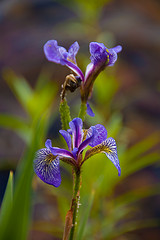
\includegraphics[width = 30mm]{01/figures/eoce/images/irisversicolor}
\end{center}
\end{minipage}
}{}

% 6

\eoce{\qt{Smoking habits of UK residents\label{UKSmoking_datamatrix}} A survey was conducted to study the smoking habits of UK residents. Below is a data matrix displaying a portion of the data collected in this survey. Note that ``$\pounds$" stands for British Pounds Sterling, ``cig" stands for cigarettes, and ``N/A'' refers to a missing component of the data. \footfullcite{data:smoking}
\begin{table}[h]
\begin{center}
\scriptsize{
\begin{tabular}{rccccccc}
  \hline
 & gender & age & marital & grossIncome & smoke & amtWeekends & amtWeekdays \\ 
  \hline
1 & Female &  42 & Single & Under $\pounds$2,600 & Yes &  12 cig/day &  12 cig/day \\ 
2 & Male &  44 & Single & $\pounds$10,400 to $\pounds$15,600 & No & N/A & N/A \\ 
3 & Male &  53 & Married & Above $\pounds$36,400 & Yes &   6 cig/day &   6 cig/day \\ 
\vdots & \vdots &  \vdots & \vdots & \vdots & \vdots & \vdots & \vdots \\ 
1691 & Male &  40 & Single & $\pounds$2,600 to $\pounds$5,200 & Yes &   8 cig/day &   8 cig/day \\   
   \hline
\end{tabular}
}
\end{center}
\end{table}
\begin{parts}
\item What does each row of the data matrix represent?
\item How many participants were included in the survey?
\item Indicate whether each variable in the study is numerical or categorical. If numerical, identify as continuous or discrete. If categorical, indicate if the variable is ordinal.
\end{parts}
}{}


%_________________
\subsection{Overview of data collection principles}

% 7

\eoce{\qt{Generalizability and causality, Part I} Identify the population of interest and the sample in the studies described in Exercise~\ref{components1}. Also comment on whether or not the results of the study can be generalized to the population and if the findings of the study can be used to establish causal relationships.
}{}

% 8

\eoce{\qt{Generalizability and causality, Part II} Identify the population of interest and the sample in the studies described in Exercise~\ref{components2}. Also comment on whether or not the results of the study can be generalized to the population and if the findings of the study can be used to establish causal relationships.
}{}

% 9
\textA{\pagebreak}

\eoce{\qt{GPA and study time} A survey was conducted on 218 undergraduates from Duke University who took an introductory statistics course in Spring 2012. Among many other questions, this survey asked them about their GPA and the number of hours they spent studying per week. The scatterplot below displays the relationship between these two variables.

\noindent\begin{minipage}[c]{0.44\textwidth}
\begin{parts}
\item What is the explanatory variable and what is the response variable?
\item Describe the relationship between the two variables. Make sure to discuss unusual observations, if any.
\item Is this an experiment or an observational study?
\item Can we conclude that studying longer hours leads to higher GPAs?
\end{parts} \vspacePE{4mm}
\end{minipage}
\begin{minipage}[c]{0.55\textwidth}
\begin{center}
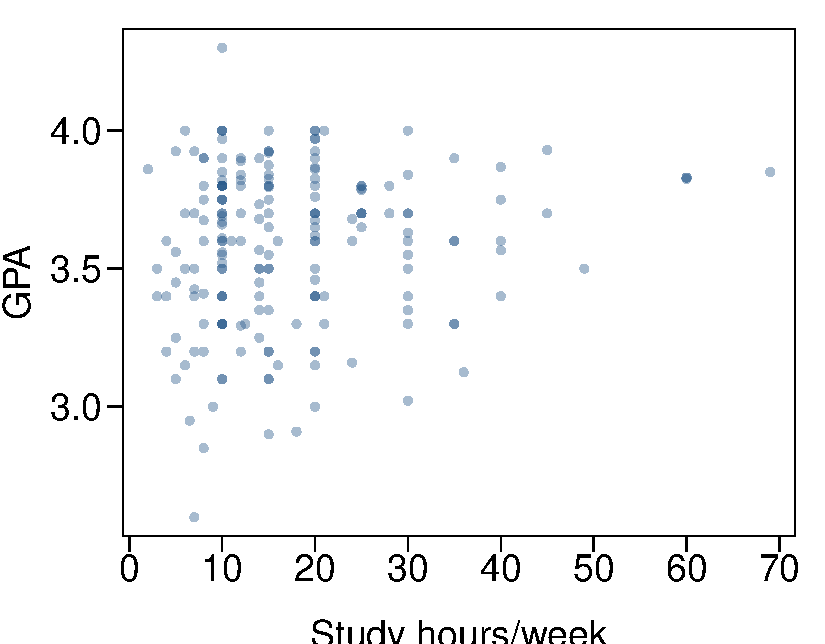
\includegraphics[width = 0.88\textwidth]{01/figures/eoce/gpaStudy/gpaStudy}
\end{center}
\end{minipage}
}{}


% 10

\eoce{\qt{Income and education} The scatterplot below shows the relationship between per capita income (in thousands of dollars) and percent of population with a bachelor's degree in 3,143 counties in the US in 2010.

\noindent\begin{minipage}[c]{0.44\textwidth}
\begin{parts}
\item What are the explanatory and response variables?
\item Describe the relationship between the two variables. Make sure to discuss unusual observations, if any.
\item Can we conclude that having a bachelor's degree increases one's income?
\end{parts} \vspacePE{16mm}
\end{minipage}
\begin{minipage}[c]{0.55\textwidth}
\begin{center}
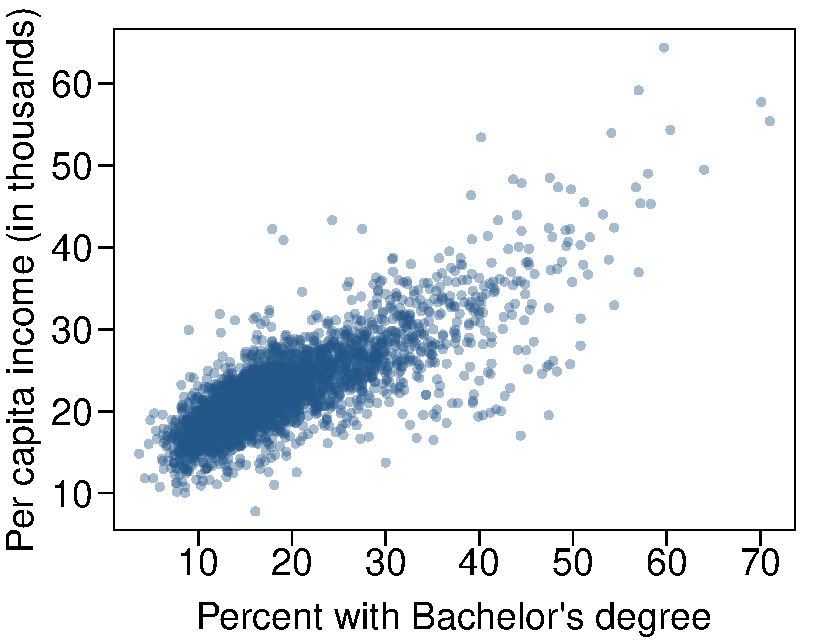
\includegraphics[width = 0.88\textwidth]{01/figures/eoce/county/county_incomeBach}
\end{center}
\end{minipage}
}{}


%_________________
\subsection{Observational studies and sampling strategies}

% 11

\eoce{\qt{Propose a sampling strategy} A large college class has 160 students. All 160 students attend the lectures together, but the students are divided into 4 groups, each of 40 students, for lab sections administered by different teaching assistants. The professor wants to conduct a survey about how satisfied the students are with the course, and he believes that the lab section a student is in might affect the student's overall satisfaction with the course.
\begin{parts}
\item What type of study is this?
\item Suggest a sampling strategy for carrying out this study.
\end{parts}
}{}


% 12
\textA{\pagebreak}

\eoce{\qt{Internet use and life expectancy} The scatterplot below shows the relationship between estimated life expectancy at birth as of 2012\footfullcite{data:ciaFactBookLifeExp:2012} and percentage of internet users in 2010\footfullcite{data:ITU:2012} in 208 countries.

\noindent\begin{minipage}[c]{0.43\textwidth}
\begin{parts}
\item Describe the relationship between life expectancy and percentage of internet users.
\item What type of study is this?
\item State a possible confounding variable that might explain this relationship and describe its potential effect.
\end{parts}\vspace{16mm}
\end{minipage}%
\begin{minipage}[r]{0.55\textwidth}
\hfill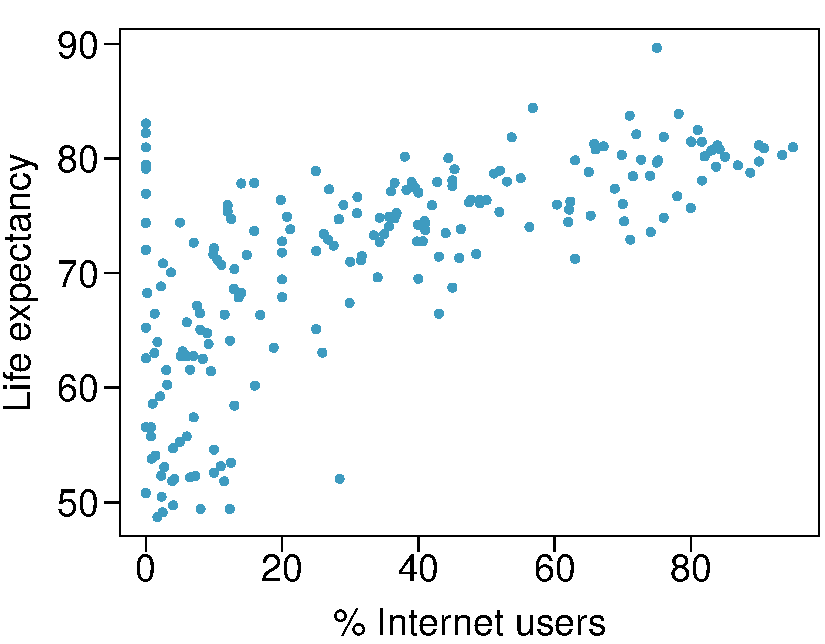
\includegraphics[width = 0.95\textwidth]{01/figures/eoce/country/county_lifeExpInter}
\end{minipage}
}{}

% 13

\eoce{\qt{Random digit dialing} The Gallup Poll uses a procedure called random digit dialing, which creates phone numbers based on a list of all area codes in America in conjunction with the associated number of residential households in each area code. Give a possible reason the Gallup Poll chooses to use random digit dialing instead of picking phone numbers from the phone book.
}{}

% 14

\eoce{\qt{Sampling strategies} A statistics student who is curious about the relationship between the amount of time students spend on social networking sites and their performance at school decides to conduct a survey. Three research strategies for collecting data are described below. In each, name the sampling method proposed and any bias you might expect.
\begin{parts}
\item He randomly samples 40 students from the study's population, gives them the survey, asks them to fill it out and bring it back the next day.
\item He gives out the survey only to his friends, and makes sure each one of them fills out the survey.
\item He posts a link to an online survey on his Facebook wall and asks his friends to fill out the survey.
\APVersion{\item He stands outside the student center and asks every third person that walks out the door to fill out the survey.}
\end{parts}
}{}


% 15

\eoce{\qt{Family size} Suppose we want to estimate family size, where family is defined as one or more parents living with children. If we select students at random at an elementary school and ask them what their family size is, will our average be biased? If so, will it overestimate or underestimate the true value?
}{}


\textA{\newpage}

% 16

\eoce{\qt{Flawed reasoning} Identify the flaw in reasoning in the following scenarios. Explain what the individuals in the study should have done differently if they wanted to make such strong conclusions.
\begin{parts}
\item Students at an elementary school are given a questionnaire that they are required to return after their parents have completed it. One of the questions asked is, ``Do you find that your work schedule makes it difficult for you to spend time with your kids after school?" Of the parents who replied, 85\% said ``no". Based on these results, the school officials conclude that a great majority of the parents have no difficulty spending time with their kids after school.
\item A survey is conducted on a simple random sample of 1,000 women who recently gave birth, asking them about whether or not they smoked during pregnancy. A follow-up survey asking if the children have respiratory problems is conducted 3 years later, however, only 567 of these women are reached at the same address. The researcher reports that these 567 women are representative of all mothers.
\item An orthopedist administers a questionnaire to 30 of his patients who do not have any joint problems and finds that 20 of them regularly go running. He concludes that running decreases the risk of joint problems.
\end{parts}
}{}


% 17

\eoce{\qt{Reading the paper} Below are excerpts from two articles published in the \emph{NY Times}:
\begin{parts}
\item An article called \emph{Risks: Smokers Found More Prone to Dementia} states the following: \footfullcite{news:smokingDementia}
\begin{adjustwidth}{2em}{2em}
{\footnotesize ``Researchers analyzed the data of 23,123 health plan members who participated in a voluntary exam and health behavior survey from 1978 to 1985, when they were 50 to 60 years old. Twenty-three years later, about one-quarter of the group, or 5,367, had dementia, including 1,136 with Alzheimer�s disease and 416 with vascular dementia. After adjusting for other factors, the researchers concluded that pack-a-day smokers were 37 percent more likely than nonsmokers to develop dementia, and the risks went up sharply with increased smoking; 44 percent for one to two packs a day; and twice the risk for more than two packs."}
\end{adjustwidth}
Based on this study, can we conclude that smoking causes dementia later in life? Explain your reasoning.
\item Another article called \emph{The School Bully Is Sleepy} states the following: \footfullcite{news:bullySleep}
\begin{adjustwidth}{2em}{2em}
{\footnotesize ``The University of Michigan study, collected survey data from parents on each child's sleep habits and asked both parents and teachers to assess behavioral concerns. About a third of the students studied were identified by parents or teachers as having problems with disruptive behavior or bullying. The researchers found that children who had behavioral issues and those who were identified as bullies were twice as likely to have shown symptoms of sleep disorders."}
\end{adjustwidth}
A friend of yours who read the article says, ``The study shows that sleep disorders lead to bullying in school children." Is this statement justified? If not, how best can you describe the conclusion that can be drawn from this study?
\end{parts}
}{}


% 18

\eoce{\qt{Shyness on Facebook} Given the anonymity afforded to individuals in online interactions, researchers hypothesized that shy individuals would have more favorable attitudes toward Facebook and that shyness would be positively correlated with time spent on Facebook. They also hypothesized that shy individuals would have fewer Facebook ``Friends" just like they have fewer friends than non-shy individuals have in the offline world. Data were collected on 103 undergraduate students at a university in southwestern Ontario via online questionnaires. The study states ``Participants were recruited through the university's psychology participation pool. After indicating an interest in the
study, participants were sent an e-mail containing the study's URL as well as the necessary login credentials." Are the results of this study generalizable to the population of all Facebook users? \footfullcite{Orr:2009}
}{}


%_________________
\subsection{Experiments}

% 19

\eoce{\qt{Vitamin supplements} In order to assess the effectiveness of taking large doses of vitamin C in reducing the duration of the common cold, researchers recruited 400 healthy volunteers from staff and students at a university. A quarter of the patients were assigned a placebo, and the rest were evenly divided between 1g Vitamin C,  3g Vitamin C, or 3g Vitamin C plus additives to be taken at onset of a cold for the following two days. All tablets had identical appearance and packaging. The nurses who handed the prescribed pills to the patients knew which patient received which treatment, but the researchers assessing the patients when they were sick did not. No significant differences were observed in any measure of cold duration or severity between the four medication groups, and the placebo group had the shortest duration of symptoms.\footfullcite{Audera:2001}
\begin{parts}
\item Was this an experiment or an observational study? Why?
\item What are the explanatory and response variables in this study?
\item Were the patients blinded to their treatment?
\item Was this study double-blind?
\item Participants are ultimately able to choose whether or not to use the pills prescribed to them. We might expect that not all of them will adhere and take their pills. Does this introduce a confounding variable to the study? Explain your reasoning.
\end{parts}
}{}


% 20

\eoce{\qt{Soda preference} You would like to conduct an experiment in class to see if your classmates prefer the taste of regular Coke or Diet Coke. Briefly outline a design for this study.
}{}


% 21

\eoce{\qt{Exercise and mental health} A researcher is interested in the effects of exercise on mental health and he proposes the following study: Use stratified random sampling to ensure representative proportions of 18-30, 31-40 and 41-55 year olds from the population. Next, randomly assign half the subjects from each age group to exercise twice a week, and instruct the rest not to exercise. Conduct a mental health exam at the beginning and at the end of the study, and compare the results.
\begin{parts}
\item What type of study is this? 
\item What are the treatment and control groups in this study?
\item Does this study make use of blocking? If so, what is the blocking variable?
\item Does this study make use of blinding?
\item Comment on whether or not the results of the study can be used to establish a causal relationship between exercise and mental health, and indicate whether or not the conclusions can be generalized to the population at large.
\item Suppose you are given the task of determining if this proposed study should get funding. Would you have any reservations about the study proposal?
\end{parts}
}{}


% 22
\textA{\newpage}

\eoce{\qt{Chia seeds and weight loss} Chia Pets -- those terra-cotta figurines that sprout fuzzy green hair -- made the chia plant a household name. But chia has gained an entirely new reputation as a diet supplement.  In one 2009 study, a team of researchers recruited 38 men and divided them evenly into two groups: treatment or control. They also recruited 38 women, and they randomly placed half of these participants into the treatment group and the other half into the control group. One group was given 25 grams of chia seeds twice a day, and the other was given a placebo. The subjects volunteered to be a part of the study. After 12 weeks, the scientists found no significant difference between the groups in appetite or weight loss. \footfullcite{Nieman:2009}
\begin{parts}
\item What type of study is this? 
\item What are the experimental and control treatments in this study?
\item Has blocking been used in this study? If so, what is the blocking variable?
\item Has blinding been used in this study?
\item Comment on whether or not we can make a causal statement, and indicate whether or not we can generalize the conclusion to the population at large.
\end{parts}
}{}


%_________________
\subsection{Examining numerical data}

% 23

\eoce{\qt{Mammal life spans} Data were collected on life spans (in years) and gestation lengths (in days) for 62 mammals. A scatterplot of life span versus length of gestation is shown below. \footfullcite{Allison+Cicchetti:1975}

\noindent\begin{minipage}[c]{0.5\textwidth}
\begin{parts}
\item What type of an association is apparent between life span and length of gestation?
\item What type of an association would you expect to see if the axes of the plot were reversed, i.e. if we plotted length of gestation versus life span?
\item Are life span and length of gestation independent? Explain your reasoning.
\end{parts} \vspace{9mm}
\end{minipage}
\begin{minipage}[c]{0.5\textwidth}
\begin{center}
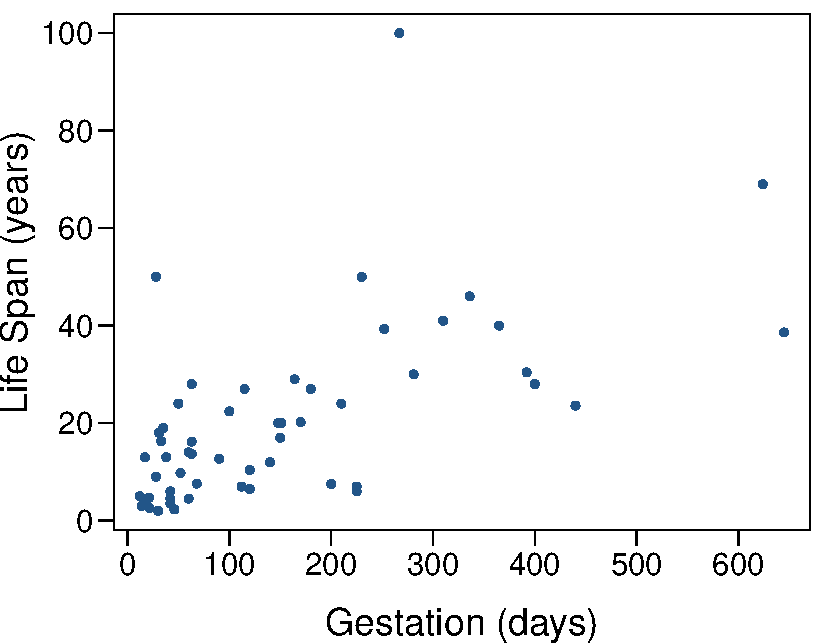
\includegraphics[width = 60mm]{01/figures/eoce/mammals/mammals_lifeSpanGest}
\end{center}
\end{minipage}
}{}


% 24

\eoce{\qt{Office productivity} Office productivity is relatively low when the employees feel no stress about their work or job security. However, high levels of stress can also lead to reduced employee productivity. Sketch a plot to represent the relationship between stress and productivity.
}{}


% 25
\textA{\newpage}

\eoce{\qt{Associations} Indicate which of the plots show a \\[1mm]
\noindent\begin{minipage}[b]{0.35\textwidth}
\begin{parts}
\item positive association
\item negative association
\item no association
\end{parts}
Also determine if the positive and negative associations are linear or nonlinear. Each part may refer to more than one plot. \vspace{31mm}
\end{minipage}%
\begin{minipage}[b]{0.62\textwidth}
\hfill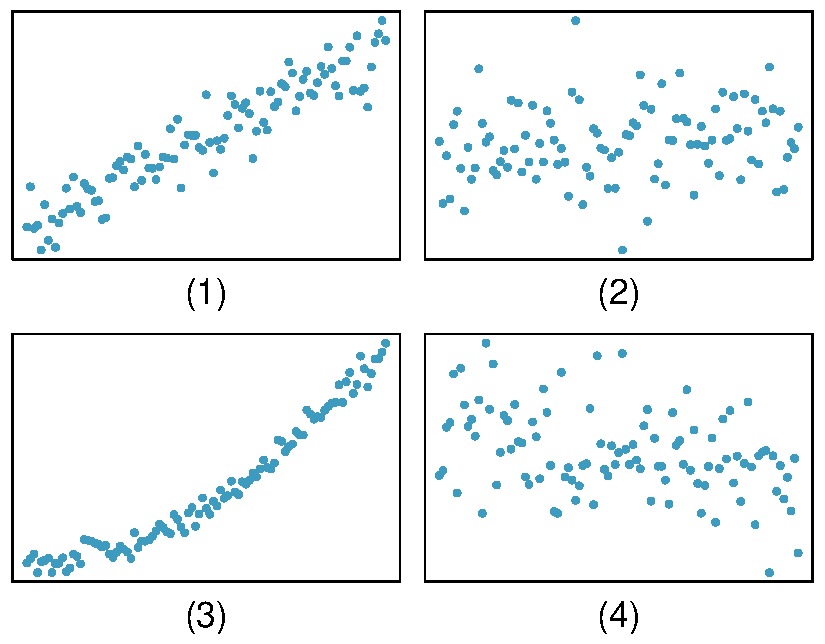
\includegraphics[width = 0.95\textwidth]{01/figures/eoce/associationPlots/associationPlots}
\end{minipage}
}{}



% 26

\eoce{\qt{Parameters and statistics} Identify which value represents the sample mean and which value represents the claimed population mean.
\begin{parts}
\item A recent article in a college newspaper stated that college students get an average of 5.5 hrs of sleep each night. A student who was skeptical about this value decided to conduct a survey by randomly sampling 25 students. On average, the sampled students slept 6.25 hours per night.
\item American households spent an average of about \$52 in 2007 on Halloween merchandise such as costumes, decorations and candy. To see if this number had changed, researchers conducted a new survey in 2008 before industry numbers were reported. The survey included 1,500 households and found that average Halloween spending was \$58 per household.
\item The average GPA of students in 2001 at a private university was 3.37. A survey on a sample of 203 students from this university yielded an average GPA of 3.59 in Spring semester of 2012.
\end{parts}
}{}


% 27

\eoce{\qt{Make-up exam} In a class of 25 students, 24 of them took an exam in class and 1 student took a make-up exam the following day. The professor graded the first batch of 24 exams and found an average score of 74 points with a standard deviation of 8.9 points. The student who took the make-up the following day scored 64 points on the exam.
\begin{parts}
\item Does the new student's score increase or decrease the average score?
\item What is the new average?
\item Does the new student's score increase or decrease the standard deviation of the scores?
\end{parts}
}{}


% 28

\eoce{\qt{Days off at a mining plant} Workers at a particular mining site receive an average of 35 days paid vacation, which is lower than the national average. The manager of this plant is under pressure from a local union to increase the amount of paid time off. However, he does not want to give more days off to the workers because that would be costly. Instead he decides he should fire 10 employees in such a way as to raise the average number of days off that are reported by his employees. In order to achieve this goal, should he fire employees who have the most number of days off, least number of days off, or those who have about the average number of days off?
}{}


% 29
\textA{\newpage}

\eoce{\qt{Smoking habits of UK residents, Part I\label{UKSmoking_amounts}} Exercise~\ref{UKSmoking_datamatrix} introduces a data set on the smoking habits of UK residents. Below are histograms displaying the distributions of the number of cigarettes smoked on weekdays and weekends, excluding non-smokers. Describe the two distributions and compare them.
\begin{center}
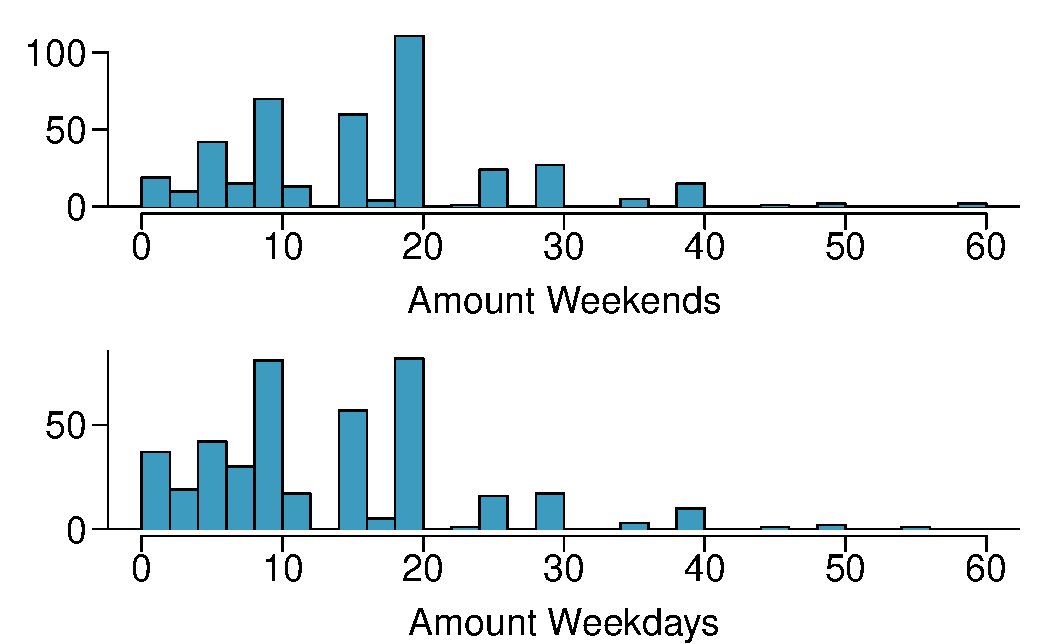
\includegraphics[width = 0.7\textwidth]{01/figures/eoce/smoking/smoking_amountHist}
\end{center}
}{}


% 30

\eoce{\qt{Stats scores\label{introStatsFinalScores}} Below are the final scores of 20 introductory statistics students.
\begin{center}
79, 83, 57, 82, 94, 83, 72, 74, 73, 71, \\
66, 89, 78, 81, 78, 81, 88, 69, 77, 79
\end{center}
Draw a histogram of these data and describe the distribution.
}{}


% 31

\eoce{\qt{Smoking habits of UK residents, Part II} A random sample of 5 smokers from the data set discussed in Exercises~\ref{UKSmoking_datamatrix} and \ref{UKSmoking_amounts} is provided below.
{\footnotesize
\begin{center}
\begin{tabular}{ccccccc}
  \hline
gender & age & maritalStatus & grossIncome & smoke & amtWeekends & amtWeekdays \\ 
  \hline
Female &  51 & Married & $\pounds$2,600 to $\pounds$5,200 & Yes &  20 cig/day &  20 cig/day\\ 
  Male &  24 & Single & $\pounds$10,400 to $\pounds$15,600 & Yes &  20 cig/day&  15 cig/day\\ 
  Female &  33 & Married & $\pounds$10,400 to $\pounds$15,600 & Yes &  20 cig/day&  10 cig/day\\ 
  Female &  17 & Single & $\pounds$5,200 to $\pounds$10,400 & Yes &  20 cig/day&  15 cig/day\\ 
  Female &  76 & Widowed & $\pounds$5,200 to $\pounds$10,400 & Yes &  20 cig/day&  20 cig/day\\ 
   \hline
\end{tabular}
\end{center}
}
\begin{parts}
\item Find the mean amount of cigarettes smoked on weekdays and weekends by these 5 respondents.
\item Find the standard deviation of the amount of cigarettes smoked on weekdays and on weekends by these 5 respondents. Is the variability higher on weekends or on weekdays?
\end{parts}
}{}


% 32

\eoce{\qt{Factory defective rate} A factory quality control manager decides to investigate the percentage of defective items produced each day. Within a given work week (Monday through Friday) the percentage of defective items produced was 2\%, 1.4\%, 4\%, 3\%, 2.2\%.
\begin{parts}
\item Calculate the mean for these data.
\item Calculate the standard deviation for these data, showing each step in detail.
\end{parts}
}{}


% 33

\eoce{\qt{Medians and IQRs} For each part, compare distributions (1) and (2) based on their medians and IQRs. You do not need to calculate these statistics; simply state how the medians and IQRs compare. Make sure to explain your reasoning. 
\begin{multicols}{2}
\begin{parts}
\item (1) 3, 5, 6, 7, 9 \\
(2) 3, 5, 6, 7, 20
\item (1) 3, 5, 6, 7, 9 \\
(2) 3, 5, 8, 7, 9
\item (1) 1, 2, 3, 4, 5 \\
(2) 6, 7, 8, 9, 10
\item (1) 0, 10, 50, 60, 100 \\
(2) 0, 100, 500, 600, 1000
\end{parts}
\end{multicols}
}{}


% 34

\eoce{\qt{Means and SDs} For each part, compare distributions (1) and (2) based on their means and standard deviations. You do not need to calculate these statistics; simply state how the means and the standard deviations compare. Make sure to explain your reasoning. \textit{Hint:} It may be useful to sketch dot plots of the distributions.
\begin{multicols}{2}
\begin{parts}
\item (1) 3, 5, 5, 5, 8, 11, 11, 11, 13 \\
(2) 3, 5, 5, 5, 8, 11, 11, 11, 20 \\
\item (1) -20, 0, 0, 0, 15, 25, 30, 30 \\
(2) -40, 0, 0, 0, 15, 25, 30, 30
\item (1) 0, 2, 4, 6, 8, 10 \\
(2) 20, 22, 24, 26, 28, 30
\item (1) 100, 200, 300, 400, 500 \\
(2) 0, 50, 300, 550, 600
\end{parts}
\end{multicols}
}{}


% 35

\eoce{\qt{Box plot} Create a box plot for the data given in Exercise~\ref{introStatsFinalScores}. The five number summary provided below may be useful.
\begin{center}
\renewcommand\arraystretch{1.5}
\begin{tabular}{ccccc}
Min	& Q1	& Q2 (Median)	& Q3	& Max \\
\hline
57	& 72.5	& 78.5	& 82.5	& 94 \\
\end{tabular}
\end{center}
}{}


% 36

\eoce{\qt{Infant mortality} The infant mortality rate is defined as the number of infant deaths per 1,000 live births. This rate is often used as an indicator of the level of health in a country. The relative frequency histogram below shows the distribution of estimated infant death rates in 2012 for 222 countries. \footfullcite{data:ciaFactBookInfMort:2012}

\noindent\begin{minipage}[c]{0.43\textwidth}
\begin{parts}
\item Estimate Q1, the median, and Q3 from the histogram.
\item Would you expect the mean of this data set to be smaller or larger than the median? Explain your reasoning.
\end{parts}
\vspace{18mm}
\end{minipage}
\begin{minipage}[c]{0.52\textwidth}
\hfill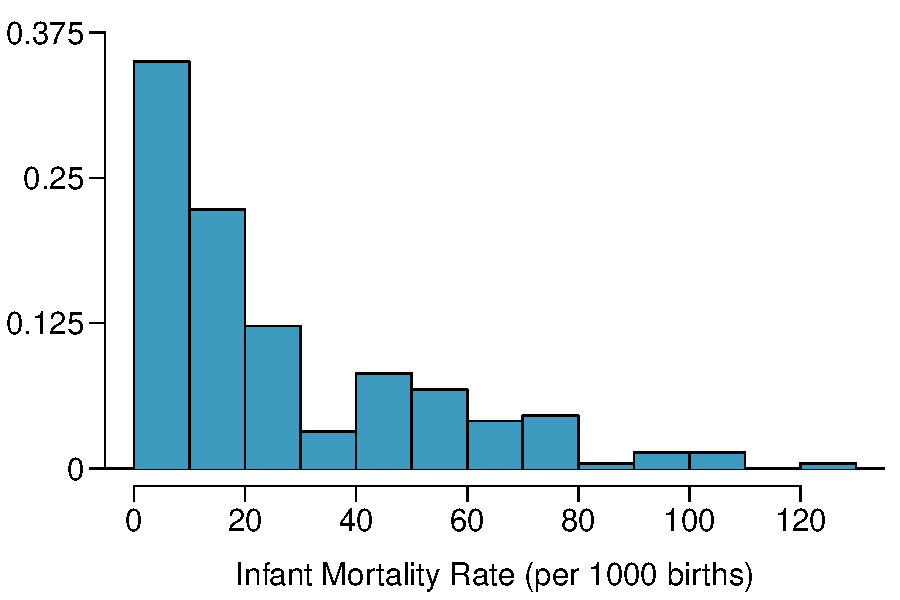
\includegraphics[width = 0.95\textwidth]{01/figures/eoce/country/country_infMort}
\end{minipage}
}{}


% 37

\eoce{\qt{Matching histograms and box plots} Describe the distribution in the histograms below and match them to the box plots. \\
\begin{center}
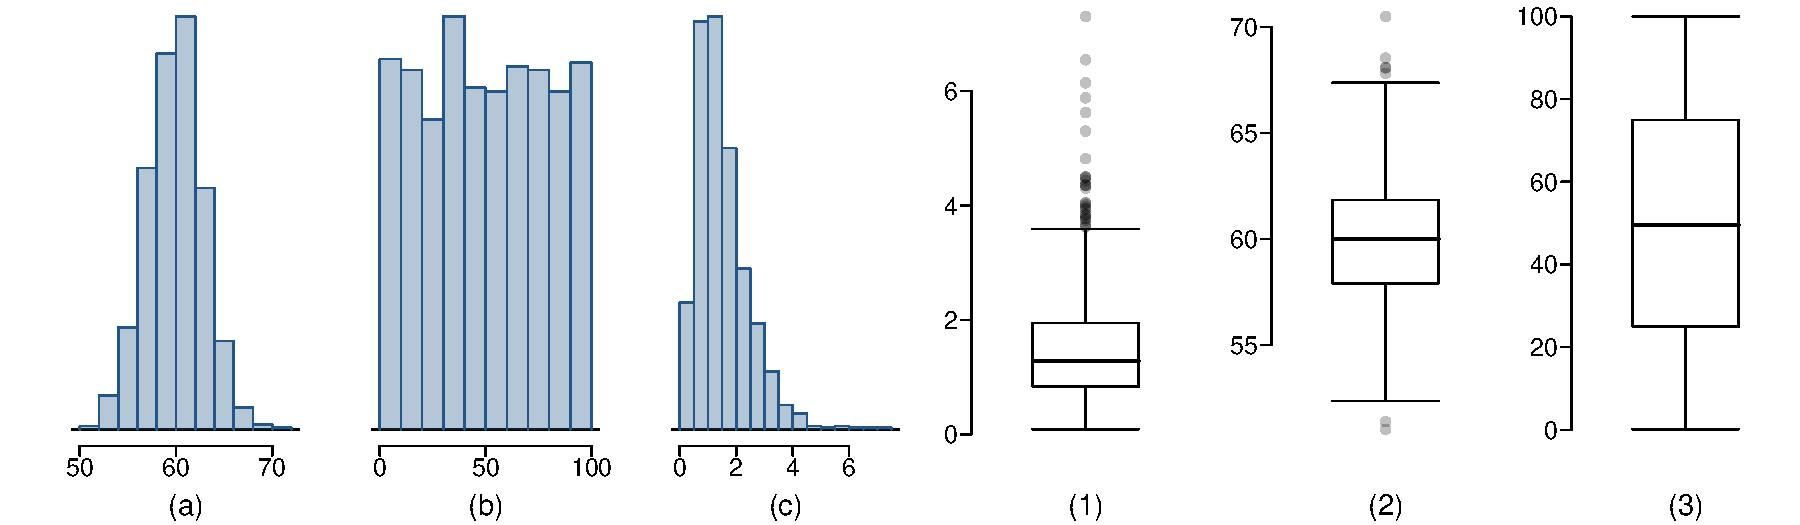
\includegraphics[width =\textwidth]{01/figures/eoce/histBoxMatch/histBoxMatch}
\end{center}
}{}


% 38
\textA{\pagebreak}

\eoce{\qt{Air quality\label{durhamAQI}} Daily air quality is measured by the air quality index (AQI) reported by the Environmental Protection Agency. This index reports the pollution level and what associated health effects might be a concern. The index is calculated for five major air pollutants regulated by the Clean Air Act. and takes values from 0 to 300, where a higher value indicates lower air quality. AQI was reported for a sample of 91 days in 2011 in Durham, NC. The relative frequency histogram below shows the distribution of the AQI values on these days. \footfullcite{data:durhamAQI:2011}
\begin{center}
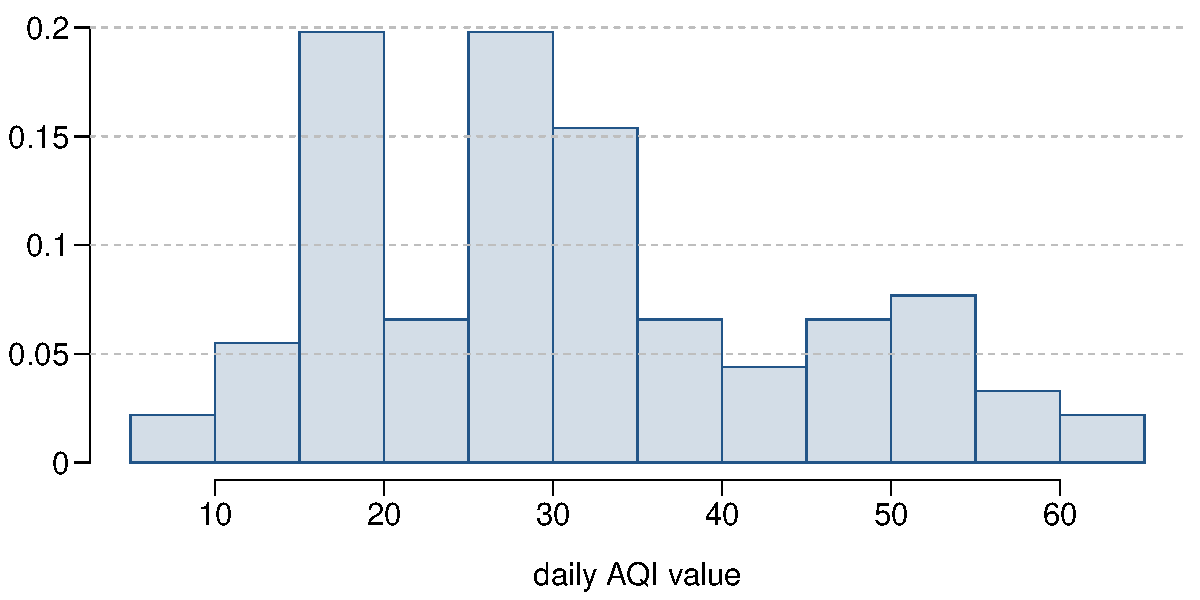
\includegraphics[width = 0.75\textwidth]{01/figures/eoce/durhamAQI/durhamAQI_hist} 
\end{center}
\begin{parts}
\item Estimate the median AQI value of this sample.
\item Would you expect the mean AQI value of this sample to be higher or lower than the median? Explain your reasoning.
\item Estimate Q1, Q3, and IQR for the distribution.
\end{parts}
}{}


% 39

\eoce{\qt{Histograms and box plots} Compare the two plots below. What characteristics of the distribution are apparent in the histogram and not in the box plot? What characteristics are apparent in the box plot but not in the histogram?
\begin{center}
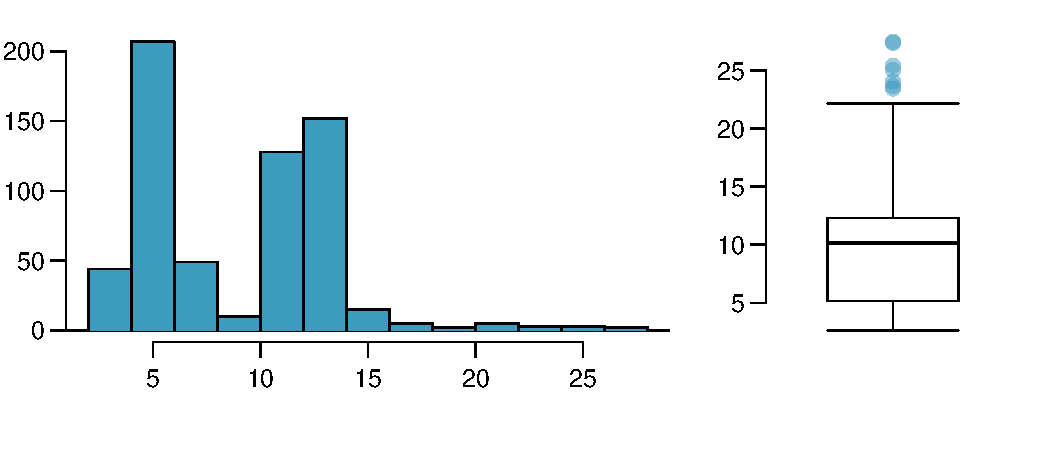
\includegraphics[width = 0.77\textwidth]{01/figures/eoce/bimodalHistBox/bimodalHistBox}
\end{center}
}{}


% 40
\textA{\pagebreak}

\eoce{\qt{Marathon winners\label{NYMarathon}} The histogram and box plots below show the distribution of finishing times for male and female winners of the New York Marathon between 1970 and 1999.
\begin{center}
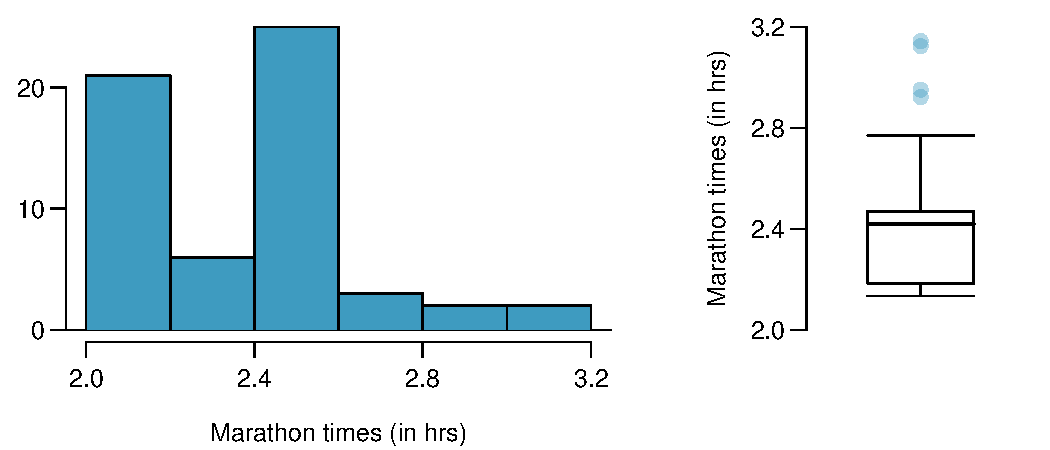
\includegraphics[width=0.9\textwidth]{01/figures/eoce/marathon/marathon_histBox}
\end{center}
\begin{parts}
\item What features of the distribution are apparent in the histogram and not the box plot? What features are apparent in the box plot but not in the histogram?
\item What may be the reason for the bimodal distribution? Explain.
\item Compare the distribution of marathon times for men and women based on the box plot shown below.
\begin{center}
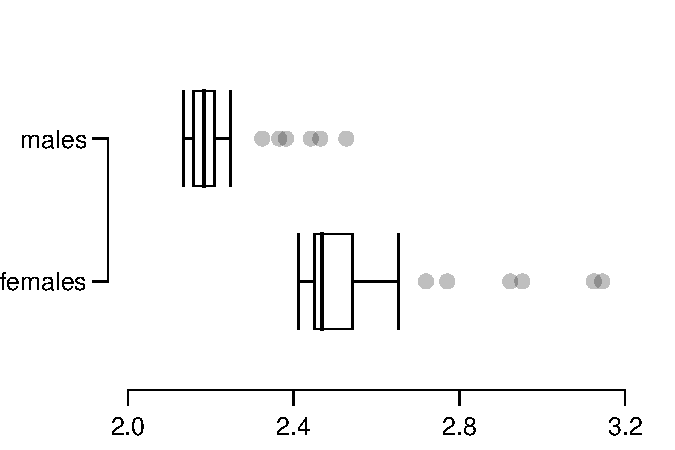
\includegraphics[width=0.7\textwidth]{01/figures/eoce/marathon/marathon_genderBox}
\end{center}
\item The time series plot shown below is another way to look at these data. Describe what is visible in this plot but not in the others.
\end{parts}
\begin{center}
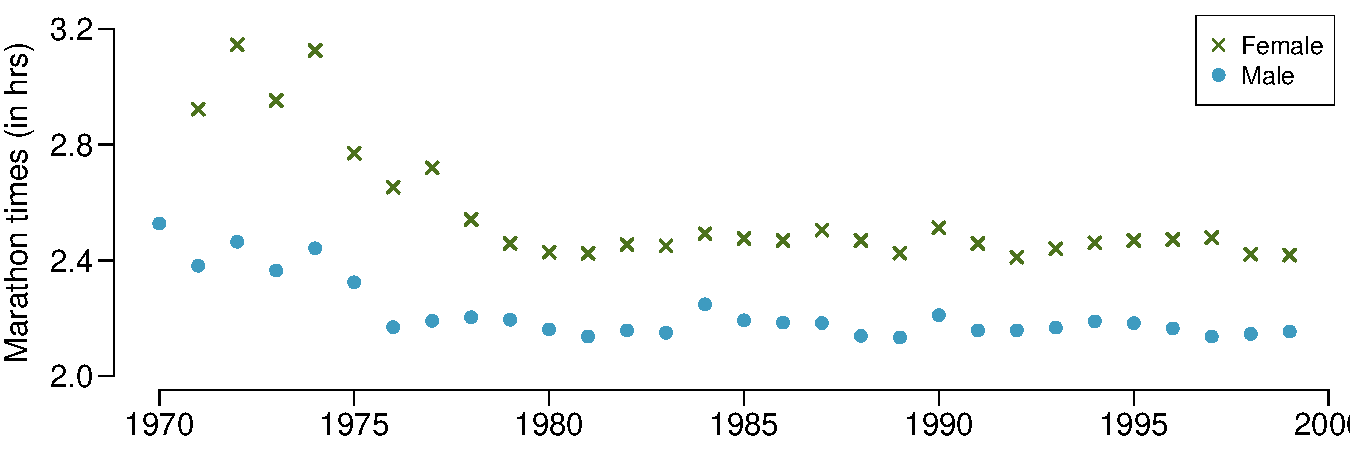
\includegraphics[width=0.95\textwidth]{01/figures/eoce/marathon/marathon_genderTimeSeries} \\
\end{center}
}{}


% 41
\textA{\pagebreak}

\eoce{\qt{Robust statistics} The first histogram below shows the distribution of the yearly incomes of 40 patrons at a college coffee shop. Suppose two new people walk into the coffee shop: one making \$225,000 and the other \$250,000. The second histogram shows the new income distribution. Summary statistics are also provided. \\
\begin{minipage}[c]{0.57\textwidth}
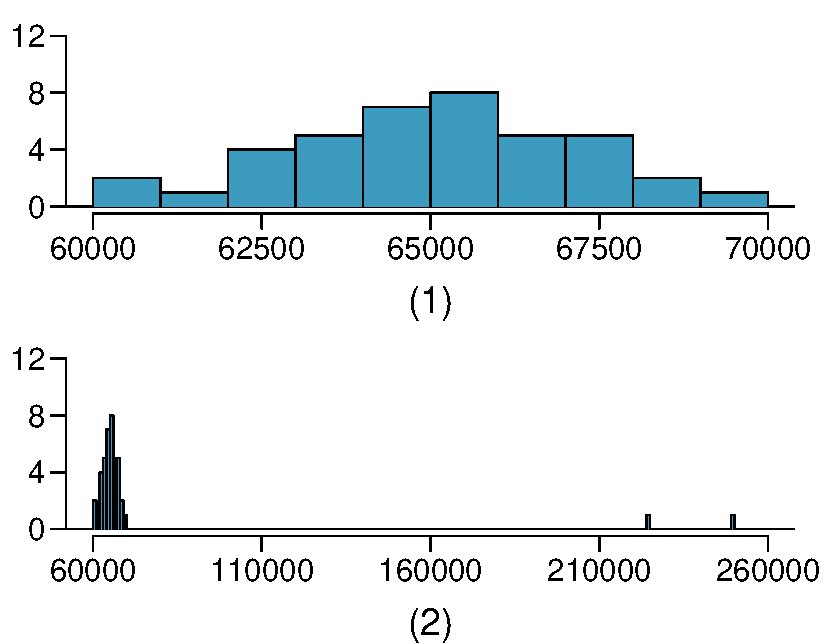
\includegraphics[width=\textwidth]{01/figures/eoce/salary/salary}
\end{minipage}
\begin{minipage}[c]{0.4\textwidth}
\begin{center}
\begin{tabular}{rrr}
  \hline
 & (1) & (2) \\ 
  \hline
n & 40 & 42 \\ 
  Min. & 60,680 & 60,680 \\ 
  1st Qu. & 63,620 & 63,710 \\ 
  Median & 65,240 & 65,350 \\ 
  Mean & 65,090 & 73,300 \\ 
  3rd Qu. & 66,160 & 66,540 \\ 
  Max. & 69,890 & 250,000 \\ 
  SD & 2,122 & 37,321 \\ 
   \hline
\end{tabular}
\end{center}
\end{minipage}
\begin{parts}
\item Would the mean or the median best represent what we might think of as a typical income for the 42 patrons at this coffee shop? What does this say about the robustness of the two measures?
\item Would the standard deviation or the IQR best represent the amount of variability in the incomes of the 42 patrons at this coffee shop? What does this say about the robustness of the two measures?
\end{parts}
}{}


% 42

\eoce{\qt{Distributions and appropriate statistics} For each of the following, describe whether you expect the distribution to be symmetric, right skewed, or left skewed. Also specify whether the mean or median would best represent a typical observation in the data, and whether the variability of observations would be best represented using the standard deviation or IQR.
\begin{parts}
\item Housing prices in a country where 25\% of the houses cost below \$350,000, 50\% of the houses cost below \$450,000, 75\% of the houses cost below \$1,000,000 and there are a meaningful number of houses that cost more than \$6,000,000.
\item Housing prices in a country where 25\% of the houses cost below \$300,000, 50\% of the houses cost below \$600,000, 75\% of the houses cost below \$900,000 and very few houses that cost more than \$1,200,000.
\item Number of alcoholic drinks consumed by college students in a given week.
\item Annual salaries of the employees at a Fortune 500 company.
\end{parts}
}{}


% 43

\noindent\begin{minipage}[c]{0.4\textwidth}
\eoce{\qt{Commuting times, Part I\label{workTravel}} The histogram to the right shows the distribution of mean commuting times in 3,143 US counties in 2010. Describe the distribution and comment on whether or not a log transformation may be advisable for these data.
}{} \vspace{5mm}
\end{minipage}%
\begin{minipage}[c]{0.58\textwidth}
\begin{center}
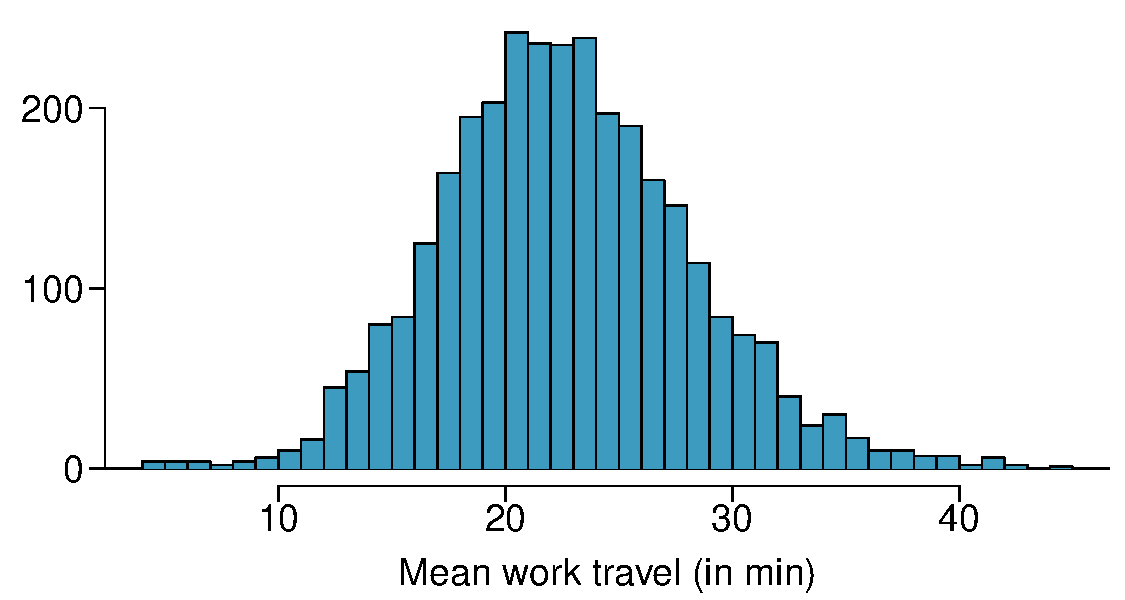
\includegraphics[width=\textwidth]{01/figures/eoce/county/county_workTravelHist}
\end{center}
\end{minipage}

\textA{\newpage}


% 44

\eoce{\qt{Hispanic population, Part I\label{hispHist}} The histogram below shows the distribution of the percentage of the population that is Hispanic in 3,143 counties in the US in 2010. Also shown is a histogram of logs of these values. Describe the distribution and comment on why we might want to use log-transformed values in analyzing or modeling these data.
\begin{center}
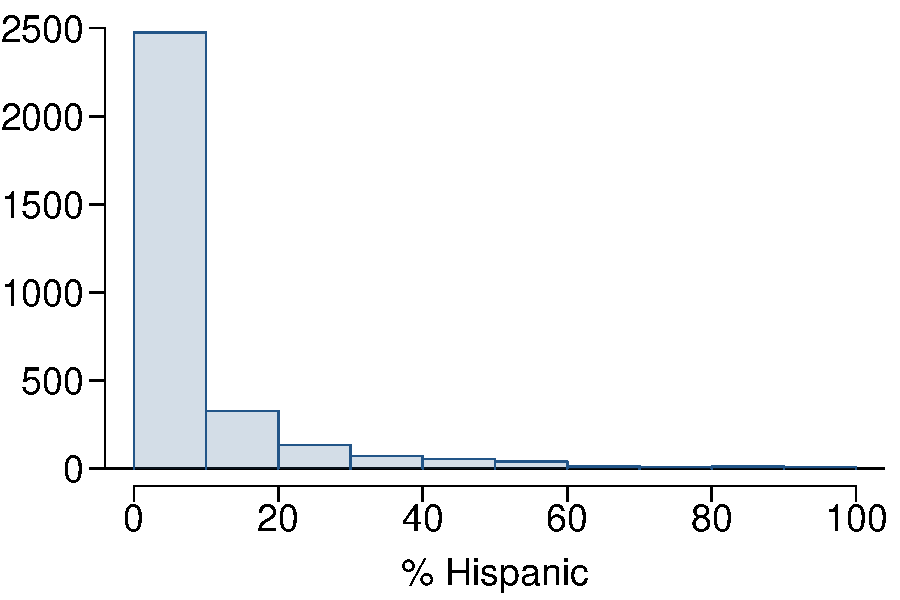
\includegraphics[width=0.49\textwidth]{01/figures/eoce/county/county_hispHist}
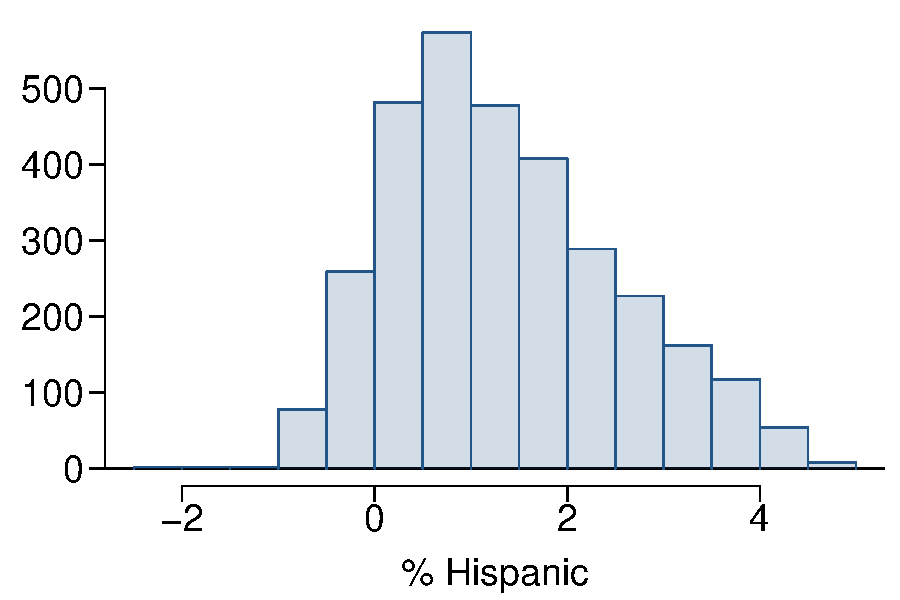
\includegraphics[width=0.49\textwidth]{01/figures/eoce/county/county_hispHistLog}
\end{center}
}{}



% 45

\eoce{\qt{Commuting times, Part II} Exercise~\ref{workTravel} displays histograms of mean commuting times in 3,143 US counties in 2010. Describe the spatial distribution of commuting times using the map below.
\begin{center}
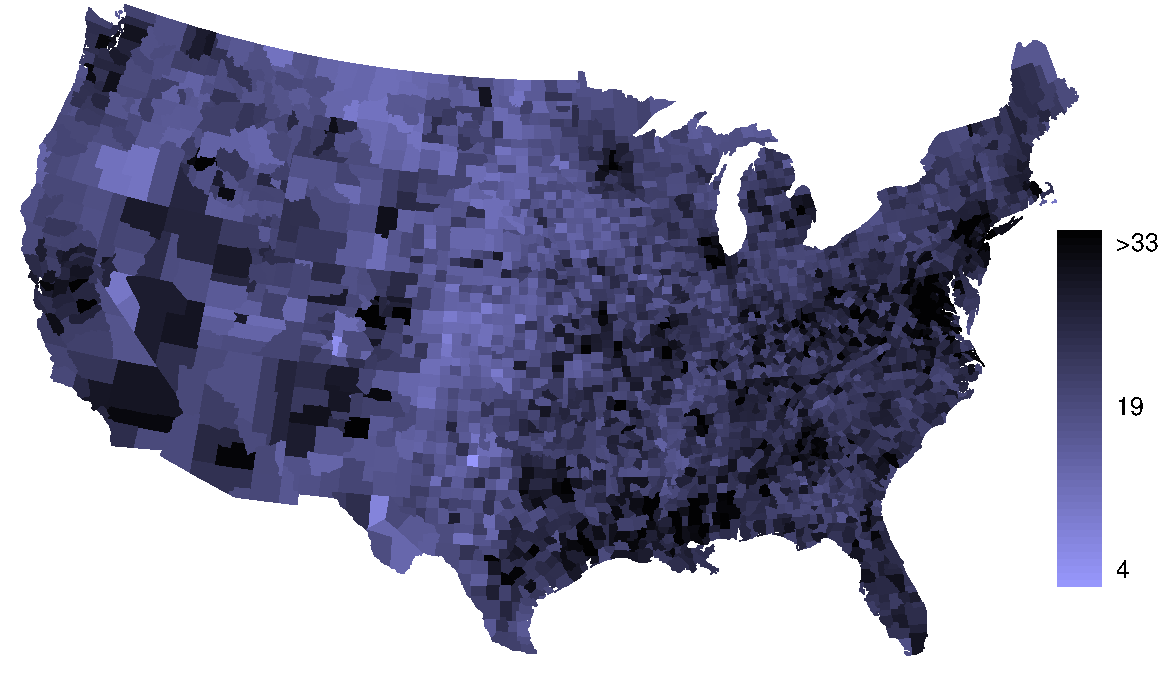
\includegraphics[width=\textwidth]{01/figures/eoce/county/county_workTravelMap}
\end{center}
}{}


% 46
\textA{\pagebreak}

\eoce{\qt{Hispanic population, Part II} Exercise~\ref{hispHist} displays histograms of the distribution of the percentage of the population that is Hispanic in 3,143 counties in the US in 2010.
\begin{center}
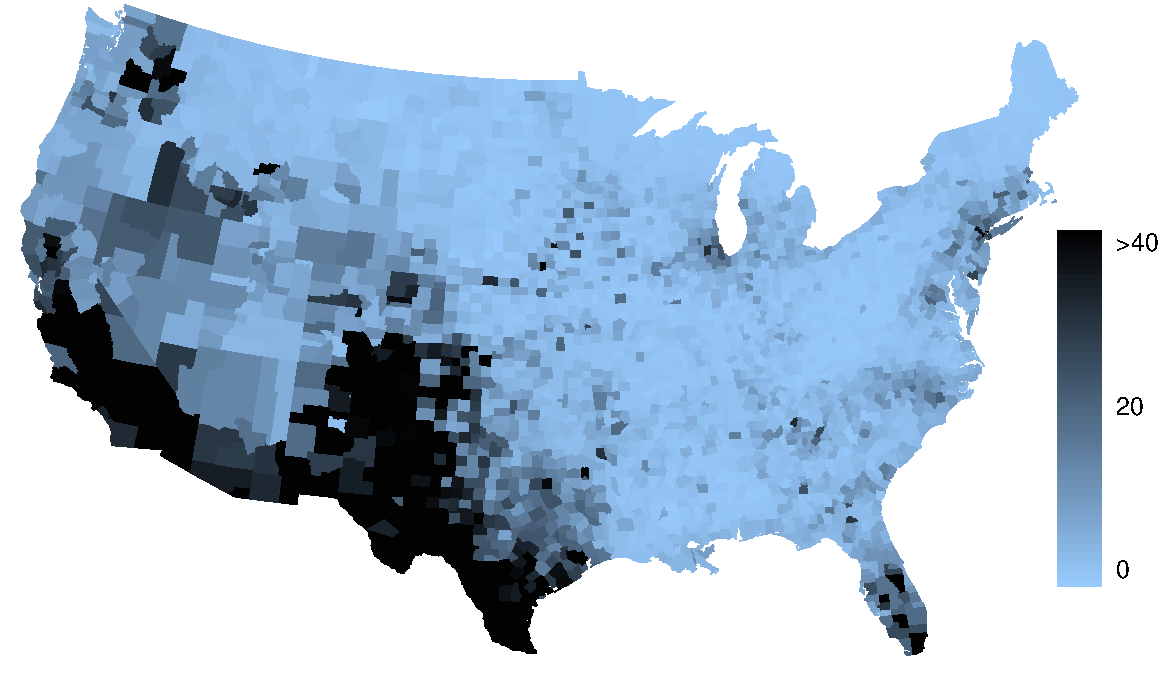
\includegraphics[width=\textwidth]{01/figures/eoce/county/county_hispMap}
\end{center}
\begin{parts}
\item What features of this distribution are apparent in the map but not in the histogram? 
\item What features are apparent in the histogram but not the map?
\item Is one visualization more appropriate or helpful than the other? Explain your reasoning.
\end{parts}
}{}


%_________________
\subsection{Considering categorical data}

% 47

\eoce{\qt{Antibiotic use in children} The bar plot and the pie chart below show the distribution of pre-existing medical conditions of children involved in a study on the optimal duration of antibiotic use in treatment of tracheitis, which is an upper respiratory infection.
\begin{parts}
\item What features are apparent in the bar plot but not in the pie chart?
\item What features are apparent in the pie chart but not in the bar plot?
\item Which graph would you prefer to use for displaying these categorical data?
\end{parts}
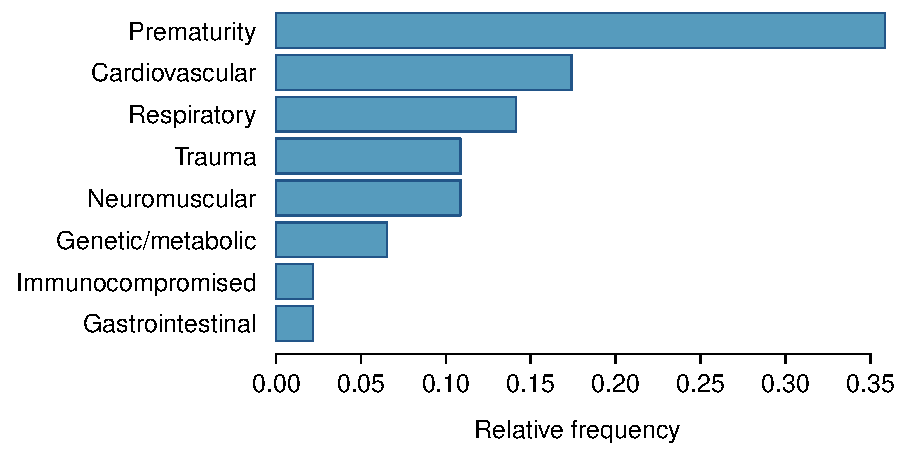
\includegraphics[width = 0.6\textwidth]{01/figures/eoce/tracheitis/tracheitis_bar}
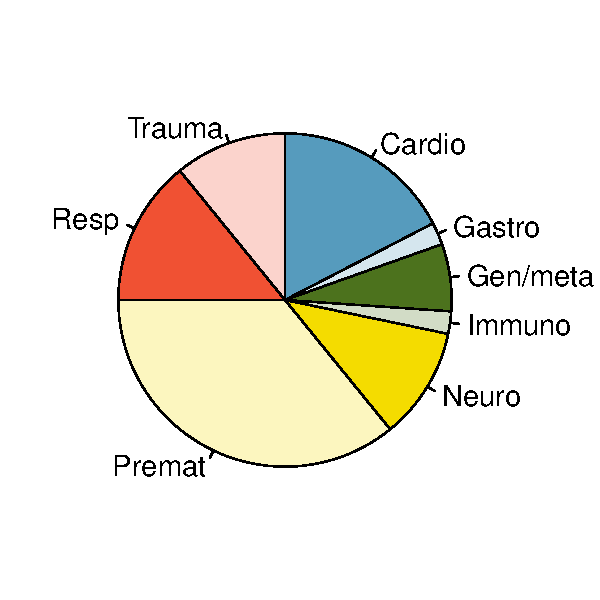
\includegraphics[width = 0.35\textwidth]{01/figures/eoce/tracheitis/tracheitis_pie}
}{}


% 48
\textA{\pagebreak}

\eoce{\qt{Views on immigration\label{immigration}} 910 randomly sampled registered voters from Tampa, FL were asked if they thought workers who have illegally entered the US should be (i) allowed to keep their jobs and apply for US citizenship, (ii) allowed to keep their jobs as temporary guest workers but not allowed to apply for US citizenship, or (iii) lose their jobs and have to leave the country. The results of the survey by political ideology are shown below.\footfullcite{survey:immigFL:2012}
\begin{center}
\begin{tabular}{l l  c c c c}
				&		& \multicolumn{3}{c}{\textit{Political ideology}} \\
\cline{3-5}
				& & Conservative	& Moderate	& Liberal 	& Total \\
\cline{2-6}
& (i) Apply for citizenship	& 57			& 120		& 101	& 278 \\
& (ii) Guest worker		& 121		& 113		& 28		& 262 \\
\raisebox{1.5ex}[0pt]{\emph{Response}} &(iii) Leave the country	& 179		& 126		& 45		& 350 \\ 
& (iv) Not sure			& 15			& 4			& 1		& 20\\
\cline{2-6}
& Total				& 372		& 363		& 175	& 910
\end{tabular}
\end{center}
\begin{parts}
\item What percent of these Tampa, FL voters identify themselves as conservatives?
\item What percent of these Tampa, FL voters are in favor of the citizenship option?
\item What percent of these Tampa, FL voters identify themselves as conservatives and are in favor of the citizenship option?
\item What percent of these Tampa, FL voters who identify themselves as conservatives are also in favor of the citizenship option? What percent of moderates and liberal share this view?
\item Do political ideology and views on immigration appear to be independent? Explain your reasoning.
\end{parts}
}{}


% 49

\noindent\begin{minipage}[c]{0.5\textwidth}
\eoce{\qt{Views on the DREAM Act} The same survey from Exercise~\ref{immigration} also asked respondents if they support the DREAM Act, a proposed law which would provide a path to citizenship for people brought illegally to the US as children. Based on the mosaic plot shown on the right, are views on the DREAM Act and political ideology independent?
}{}
\vspace{3mm}
\end{minipage}
\begin{minipage}[c]{0.5\textwidth}
\begin{center}
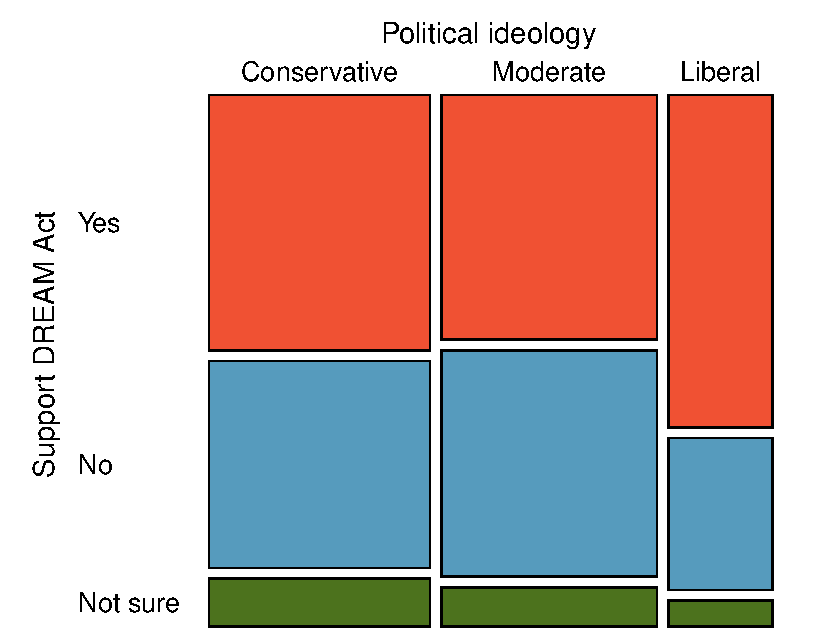
\includegraphics[width = 0.85\textwidth]{01/figures/eoce/dreamAct/dreamAct_mosaic}
\end{center}
\end{minipage} \vspace{3mm}

\textA{\newpage}

% 50

\eoce{\qt{Heart transplants, Part I\label{HeartTr}} The Stanford University Heart Transplant Study was conducted to determine whether an experimental heart transplant program increased lifespan. Each patient entering the program was designated an official heart transplant candidate, meaning that he was gravely ill and would most likely benefit from a new heart. Some patients got a transplant and some did not. The variable \texttt{transplant} indicates which group the patients were in; patients in the treatment group got a transplant and those in the control group did not. Another variable called \texttt{survived} was used to indicate whether or not the patient was alive at the end of the study. \footfullcite{Turnbull+Brown+Hu:1974}
\begin{parts}
\item Based on the mosaic plot, is survival independent of whether or not the patient got a transplant? Explain your reasoning.
\item What do the box plots suggest about the efficacy (effectiveness) of transplants?
\end{parts}
\begin{center}
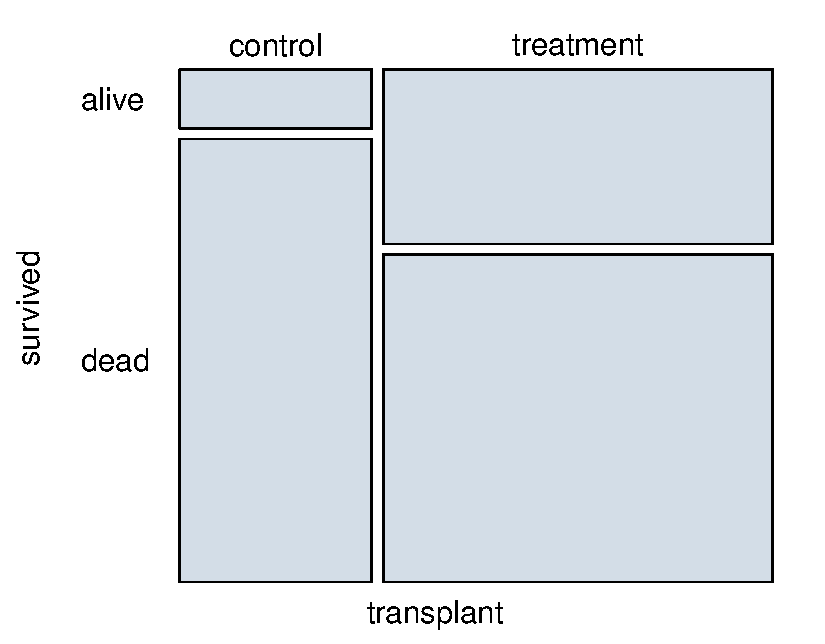
\includegraphics[width= 0.48\textwidth]{01/figures/eoce/heartTr/heartTr_SurvTrMosaic}\ 
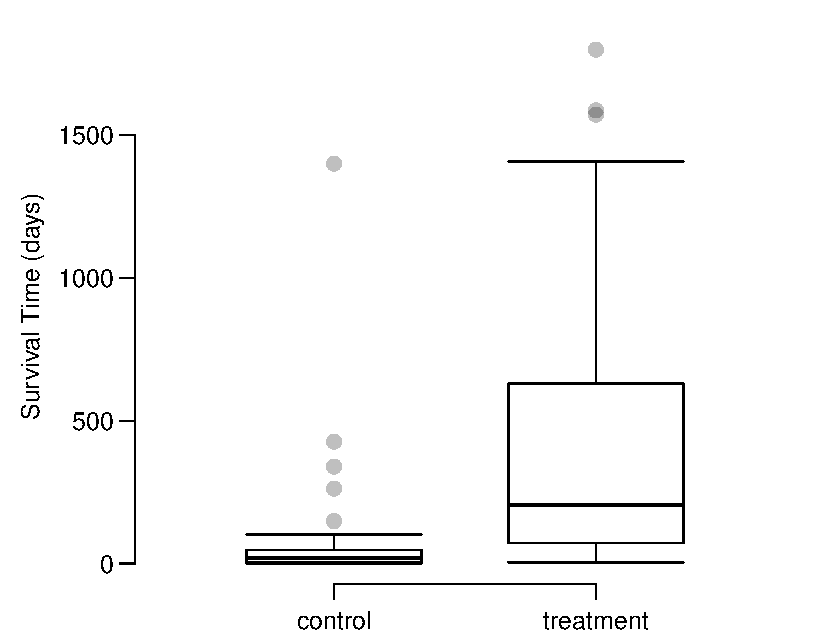
\includegraphics[width = 0.48\textwidth]{01/figures/eoce/heartTr/heartTr_SurvTimeTrBox}
\end{center}
}{}




% Chapter 2: Exploratory data analysis
\setcounter{chapter}{1}\normalsize\chapter{Exploratory Data Analysis}
\label{exploratiryDataAnalysis}

% Some chapter intro

\section{Categorical vs. categorical}

\index{data!email|(}

Like numerical data, categorical data can also be organized and analyzed. This section introduces tables and other basic tools for categorical data that are used throughout this book. The \data{email50} data set represents a sample from a larger email data set called \data{email}. This larger data set contains information on 3,921 emails. In this section we will examine whether the presence of numbers, small or large, in an email provides any useful value in classifying email as spam or not spam.
% library(openintro); data(email); dim(email)

\subsection{Contingency tables and bar plots}

Table~\ref{emailSpamNumberTableTotals} summarizes two variables: \var{spam} and \var{number}. Recall that \var{number} is a categorical variable that describes whether an email contains no numbers, only small numbers (values under 1 million), or at least one big number (a value of 1 million or more). A table that summarizes data for two categorical variables in this way is called a \term{contingency table}. Each value in the table represents the number of times a particular combination of variable outcomes occurred. For example, the value 149 corresponds to the number of emails in the data set that are spam \emph{and} had no number listed in the email. Row and column totals are also included. The \term{row totals} \index{contingency table!row totals} provide the total counts across each row (e.g. $149 + 168 + 50 = 367$), and \term{column totals} \index{contingency table!column totals} are total counts down each column.

A table for a single variable is called a \term{frequency table}. Table~\ref{emailNumberTable} is a frequency table for the \var{number} variable. If we replaced the counts with percentages or proportions, the table would be called a \term{relative frequency table}.

\begin{table}[ht]
\centering
\begin{tabular}{ll  ccc  rr}
& & \multicolumn{3}{c}{\bf \var{number}} & \\
  \cline{3-5}
& & none & small & big & Total & \hspace{2mm}\  \\ 
  \cline{2-6}
	 & spam &  149 & 168 &  50 & 367 \\ 
\raisebox{1.5ex}[0pt]{\var{spam}} 
	& not spam &  400 & 2659 & 495 & 3554 \\ 
  \cline{2-6}
& Total & 549 & 2827 & 545 & 3921 \\
  \cline{2-6}
\end{tabular}
\caption{A contingency table for \var{spam} and \var{number}.}
\label{emailSpamNumberTableTotals}
%library(openintro); library(xtable); data(email); tab <- table(email[,c("spam", "number")])[2:1,]; xtable(tab); rowSums(tab); colSums(tab); sum(tab)
\end{table}

\begin{table}[htb]
\centering
\begin{tabular}{cccc}
  \hline
none & small & big & Total \\ 
 % \hline
 549 & 2827 & 545 & 3921 \\
   \hline
\end{tabular}
\caption{A frequency table for the \var{number} variable.}
\label{emailNumberTable}
\end{table}
%library(openintro); library(xtable); data(email); xtable(table(email[,c("html")]))

A bar plot is a common way to display a single categorical variable. The left panel of Figure~\ref{emailNumberBarPlot} shows a \term{bar plot} for the \var{number} variable. In the right panel, the counts are converted into proportions (e.g. $549/3921=0.140$ for \resp{none}).

\begin{figure}[bht]
   \centering
   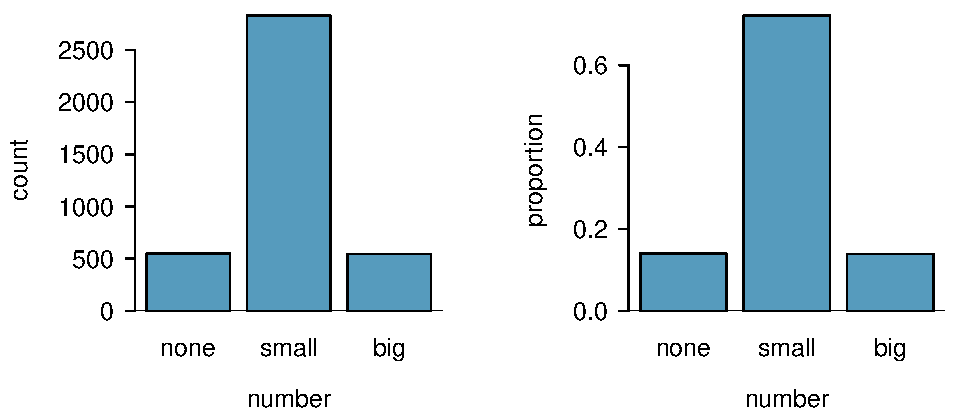
\includegraphics[width=\textwidth]{02/figures/emailNumberBarPlot/emailNumberBarPlot}
   \caption{Two bar plots of \var{number}. The left panel shows the counts, and the right panel shows the proportions in each group.}
   \label{emailNumberBarPlot}
\end{figure}


\subsection{Row and column proportions}

Table~\ref{rowPropSpamNumber} shows the row proportions for Table~\ref{emailSpamNumberTableTotals}. The \termsub{row proportions}{contingency table!row proportions} are computed as the counts divided by their row totals. The value 149 at the intersection of \resp{spam} and \resp{none} is replaced by $149/367=0.406$, i.e. 149 divided by its row total, 367. So what does 0.406 represent? It corresponds to the proportion of spam emails in the sample that do not have any numbers.

\begin{table}[ht]
\centering
\begin{tabular}{l rrr r}
  \hline
 & none & small & big & Total \\ 
  \hline
spam &  $149/367 = 0.406$ & $168/367 = 0.458$ &
			$50/367 = 0.136$ & 1.000 \\ 
not spam &  $400/3554 = 0.113$ & $2657/3554 = 0.748$ &
			$495/3554 = 0.139$ & 1.000 \\ 
   \hline
Total & $549/3921 = 0.140$ & $2827/3921 = 0.721$ &
			$545/3921 = 0.139$ & 1.000 \\
  \hline
\end{tabular}
\caption{A contingency table with row proportions for the \var{spam} and \var{number} variables.}
\label{rowPropSpamNumber}
% library(openintro); data(email); g <- table(email$spam, email$number)[2:1,]; g / rep(rowSums(g), 3); rowSums(g)
\end{table}

A contingency table of the column proportions is computed in a similar way, where each \termsub{column proportion}{contingency table!column proportion} is computed as the count divided by the corresponding column total. Table~\ref{colPropSpamNumber} shows such a table, and here the value 0.271 indicates that 27.1\% of emails with no numbers were spam. This rate of spam is much higher than emails with only small numbers (5.9\%) or big numbers (9.2\%). Because these spam rates vary between the three levels of \var{number} (\resp{none}, \resp{small}, \resp{big}), this provides evidence that the \var{spam} and \var{number} variables are associated.

\begin{table}[ht]
\centering\small
\begin{tabular}{l rrr r}
  \hline
 & none & small & big & Total \\ 
  \hline
spam &  $149/549 = 0.271$ & $168/2827 = 0.059$ &
				$50/545 = 0.092$ & $367/3921 = 0.094$ \\ 
not spam &  $400/549 = 0.729$ & $2659/2827 = 0.941$ &
				$495/545 = 0.908$ & $3684/3921 = 0.906$ \\ 
   \hline
Total & 1.000 & 1.000 & 1.000 & 1.000 \\
   \hline
\end{tabular}
\caption{A contingency table with column proportions for the \var{spam} and \var{number} variables.}
\label{colPropSpamNumber}
% library(openintro); data(email); g <- table(email$spam, email$number)[2:1,]; g / rep(colSums(g), rep(2, 3)); g; colSums(g)
\end{table}

\textPE{\pagebreak}

We could also have checked for an association between \var{spam} and \var{number} in Table~\ref{rowPropSpamNumber} using row proportions. When comparing these row proportions, we would look down columns to see if the fraction of emails with no numbers, small numbers, and big numbers varied from \resp{spam} to \resp{not~spam}.

\begin{exercise}
What does 0.458 represent in Table~\ref{rowPropSpamNumber}? What does 0.059 represent in Table~\ref{colPropSpamNumber}?\footnote{0.458 represents the proportion of spam emails that had a small number. 0.058 represents the fraction of emails with small numbers that are spam.}
\end{exercise}

\begin{exercise}
What does 0.139 at the intersection of \resp{not~spam} and \resp{big} represent in Table~\ref{rowPropSpamNumber}? What does 0.908 represent in the Table~\ref{colPropSpamNumber}?\footnote{0.139 represents the fraction of non-spam email that had a big number. 0.908 represents the fraction of emails with big numbers that are non-spam emails.}
\end{exercise}

\begin{example}{Data scientists use statistics to filter spam from incoming email messages. By noting specific characteristics of an email, a data scientist may be able to classify some emails as spam or not spam with high accuracy. One of those characteristics is whether the email contains no numbers, small numbers, or big numbers. Another characteristic is whether or not an email has any HTML content. A contingency table for the \var{spam} and \var{format} variables from the \data{email} data set are shown in Table~\ref{emailSpamHTMLTableTotals}. Recall that an HTML email is an email with the capacity for special formatting, e.g. bold text. In Table~\ref{emailSpamHTMLTableTotals}, which would be more helpful to someone hoping to classify email as spam or regular email: row or column proportions?} \label{weighingRowColumnProportions}
Such a person would be interested in how the proportion of spam changes within each email format. This corresponds to column proportions: the proportion of spam in plain text emails and the proportion of spam in HTML emails.

If we generate the column proportions, we can see that a higher fraction of plain text emails are spam ($209/1195 = 17.5\%$) than compared to HTML emails ($158/2726 = 5.8\%$). This information on its own is insufficient to classify an email as spam or not spam, as over 80\% of plain text emails are not spam. Yet, when we carefully combine this information with many other characteristics, such as \var{number} and other variables, we stand a reasonable chance of being able to classify some email as spam or not spam. \GLMSection{This is a topic we will return to in Chapter~\ref{multipleRegressionAndANOVA}.}{}
\end{example}

\begin{table}[ht]
\centering
\begin{tabular}{l cc r}
  \hline
 & text & HTML & Total \\ 
  \hline
spam & 209 & 158 & 367 \\ 
not spam & 986 & 2568 & 3554 \\ 
   \hline
Total & 1195 & 2726 & 3921 \\
   \hline
\end{tabular}
\caption{A contingency table for \var{spam} and \var{format}.}
\label{emailSpamHTMLTableTotals}
%library(openintro); library(xtable); data(email); tab <- table(email[,c("spam", "format")])[2:1,]; tab; colSums(tab); rowSums(tab)
\end{table}

Example~\ref{weighingRowColumnProportions} points out that row and column proportions are not equivalent. Before settling on one form for a table, it is important to consider each to ensure that the most useful table is constructed.

\begin{exercise}
Look back to Tables~\ref{rowPropSpamNumber} and~\ref{colPropSpamNumber}. Which would be more useful to someone hoping to identify spam emails using the \var{number} variable?\footnote{The column proportions in Table~\ref{colPropSpamNumber} will probably be most useful, which makes it easier to see that emails with small numbers are spam about 5.9\% of the time (relatively rare). We would also see that about 27.1\% of emails with no numbers are spam, and 9.2\% of emails with big numbers are spam.}
\end{exercise}

\subsection{Segmented bar and mosaic plots}
\label{segmentedBarPlotsAndIndependence}

Contingency tables using row or column proportions are especially useful for examining how two categorical variables are related. Segmented bar and mosaic plots provide a way to visualize the information in these tables.

A \termsub{segmented bar plot}{bar plot!segmented bar plot} is a graphical display of contingency table information. For example, a segmented bar plot representing Table~\ref{colPropSpamNumber} is shown in Figure~\ref{emailSpamNumberSegBar}, where we have first created a bar plot using the \var{number} variable and then separated each group by the levels of \var{spam}. The column proportions of Table~\ref{colPropSpamNumber} have been translated into a standardized segmented bar plot in Figure~\ref{emailSpamNumberSegBarSta}, which is a helpful visualization of the fraction of spam emails in each level of \var{number}.

\begin{figure}
\centering
\subfigure[]{
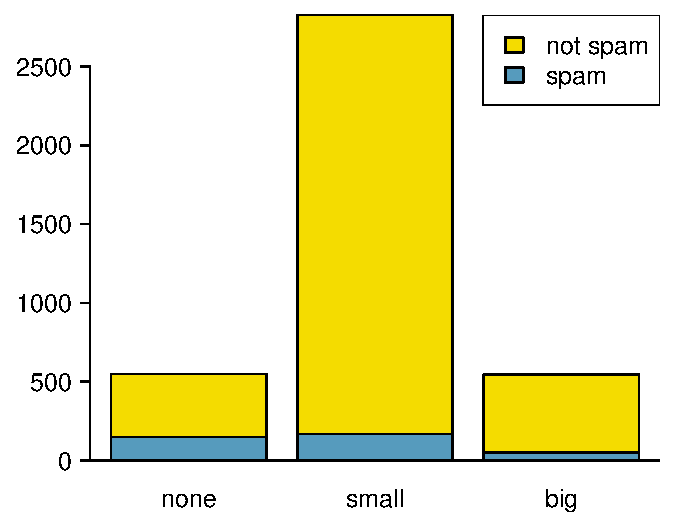
\includegraphics[width=0.46\textwidth]{02/figures/emailSpamNumberSegBar/emailSpamNumberSegBar}
\label{emailSpamNumberSegBar}
}
\subfigure[]{
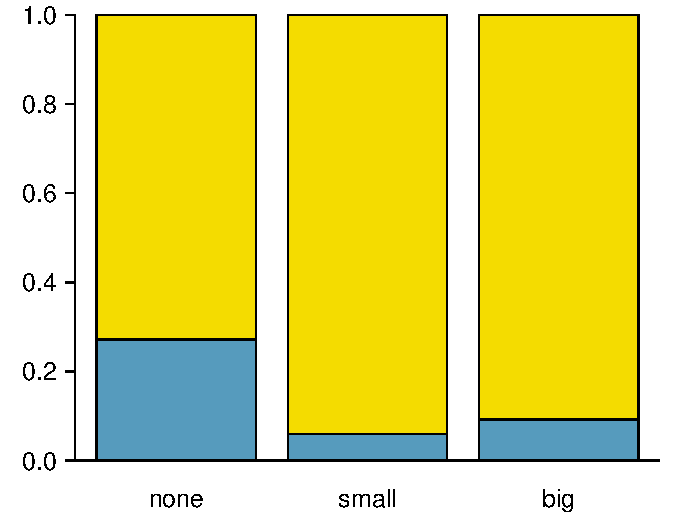
\includegraphics[width=0.46\textwidth]{02/figures/emailSpamNumberSegBar/emailSpamNumberSegBarSta}
\label{emailSpamNumberSegBarSta}
}
\caption{\subref{emailSpamNumberSegBar} Segmented bar plot for numbers found in emails, where the counts have been further broken down by \var{spam}. \subref{emailSpamNumberSegBarSta} Standardized version of Figure~\subref{emailSpamNumberSegBar}.}
\label{emailSpamNumberSegBarPlot}
\end{figure}

\begin{example}{Examine both of the segmented bar plots. Which is more useful?}
Figure~\ref{emailSpamNumberSegBar} contains more information, but Figure~\ref{emailSpamNumberSegBarSta} presents the information more clearly. This second plot makes it clear that emails with no number have a relatively high rate of spam email -- about 27\%! On the other hand, less than 10\% of email with small or big numbers are spam.
\end{example}

Since the proportion of spam changes across the groups in Figure~\ref{emailSpamNumberSegBarSta}, we can conclude the variables are dependent, which is something we were also able to discern using table proportions. Because both the \resp{none} and \resp{big} groups have relatively few observations compared to the \resp{small} group, the association is more difficult to see in Figure~\ref{emailSpamNumberSegBar}.

In some other cases, a segmented bar plot that is not standardized will be more useful in communicating important information. Before settling on a particular segmented bar plot, create standardized and non-standardized forms and decide which is more effective at communicating features of the data.

\begin{figure}
\centering
\subfigure[]{
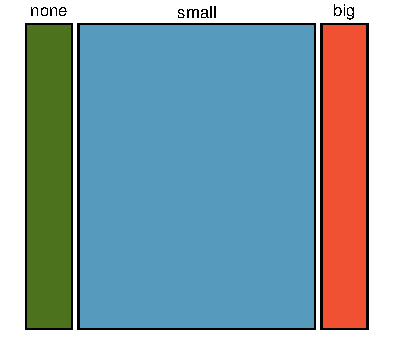
\includegraphics[width=0.4034\textwidth]{02/figures/emailSpamNumberMosaicPlot/emailNumberMosaic}
\label{emailNumberMosaic}
}
\subfigure[]{
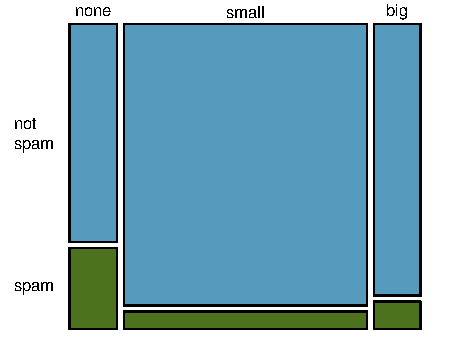
\includegraphics[width=0.4706\textwidth]{02/figures/emailSpamNumberMosaicPlot/emailSpamNumberMosaic}
\label{emailSpamNumberMosaic}
}
\caption{The one-variable mosaic plot for \var{number} and the two-variable mosaic plot for both \var{number} and \var{spam}.}
\label{emailSpamNumberMosaicPlot}
\end{figure}

A \term{mosaic plot} is a graphical display of contingency table information that is similar to a bar plot for one variable or a segmented bar plot when using two variables. Figure~\ref{emailNumberMosaic} shows a mosaic plot for the \var{number} variable. Each column represents a level of \var{number}, and the column widths correspond to the proportion of emails of each number type. For instance, there are fewer emails with no numbers than emails with only small numbers, so the no number email column is slimmer. In general, mosaic plots use box \emph{areas} to represent the number of observations.

\begin{figure}
   \centering
   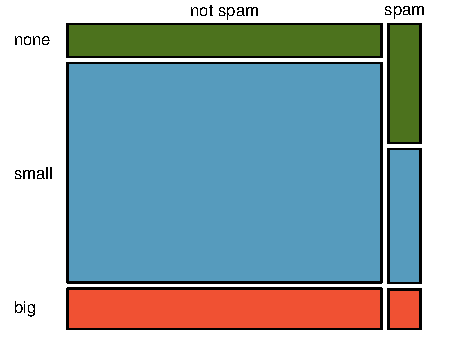
\includegraphics[width=0.45\textwidth]{02/figures/emailSpamNumberMosaicPlot/emailSpamNumberMosaicRev}
   \caption{Mosaic plot where emails are grouped by the \var{number} variable after they've been divided into \resp{spam} and \resp{not spam}.}
   \label{emailSpamNumberMosaicRev}
\end{figure}

This one-variable mosaic plot is further divided into pieces in Figure~\ref{emailSpamNumberMosaic} using the \var{spam} variable. Each column is split proportionally according to the fraction of emails that were spam in each number category. For example, the second column, representing emails with only small numbers, was divided into emails that were spam (lower) and not spam (upper). 
As another example, the bottom of the third column represents spam emails that had big numbers, and the upper part of the third column represents regular emails that had big numbers. We can again use this plot to see that the \var{spam} and \var{number} variables are associated since some columns are divided in different vertical locations than others, which was the same technique used for checking an association in the standardized version of the segmented bar plot.

In a similar way, a mosaic plot representing row proportions of Table~\ref{emailSpamNumberTableTotals} could be constructed, as shown in Figure~\ref{emailSpamNumberMosaicRev}. However, because it is more insightful for this application to consider the fraction of spam in each category of the \var{number} variable, we prefer Figure~\ref{emailSpamNumberMosaic}.

\subsection{The only pie chart you will see in this book}

While pie charts are well known, they are not typically as useful as other charts in a data analysis. A \term{pie chart} is shown in Figure~\vref{emailNumberPieChart} alongside a bar plot. It is generally more difficult to compare group sizes in a pie chart than in a bar plot, especially when categories have nearly identical counts or proportions. In the case of the \resp{none} and \resp{big} categories, the difference is so slight you may be unable to distinguish any difference in group sizes for either~plot!

\begin{figure}
   \centering
   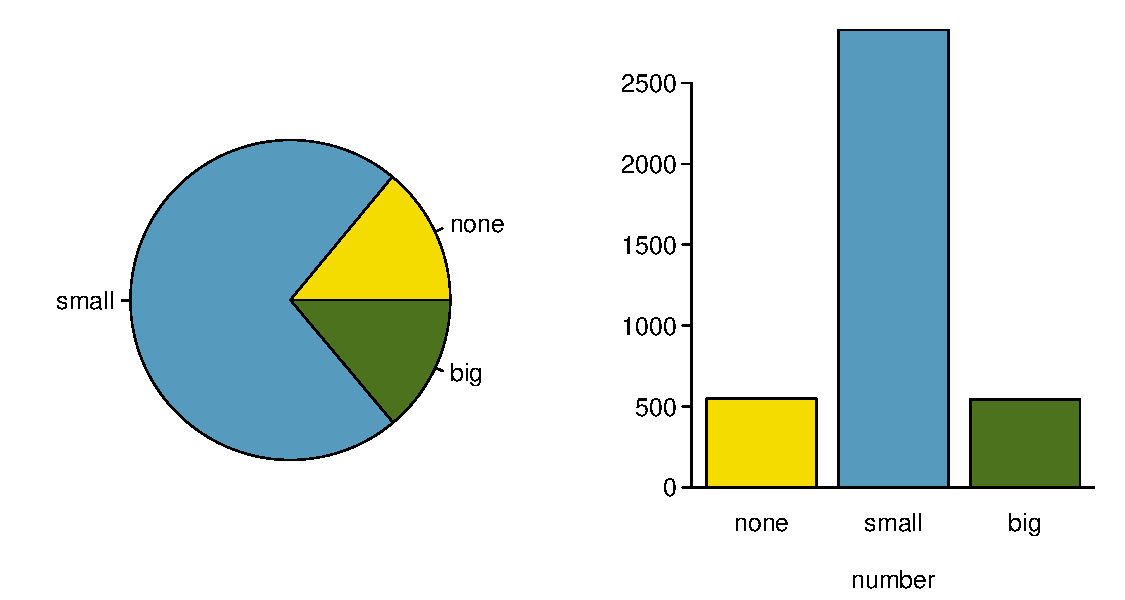
\includegraphics[width=\textwidth]{02/figures/emailNumberPieChart/emailNumberPieChart}
   \caption{A pie chart and bar plot of \var{number} for the \data{email} data set.}
   \label{emailNumberPieChart}
\end{figure}

\index{data!email|)}


\section{Numerical vs. categorical}

This section introduces techniques for exploring and summarizing numerical variables, and the \data{email50} and \data{county} data sets from Section~\ref{dataBasics} provide rich opportunities for examples. Recall that outcomes of numerical variables are numbers on which it is reasonable to perform basic arithmetic operations. For example, the \var{pop2010} variable, which represents the populations of counties in 2010, is numerical since we can sensibly discuss the difference or ratio of the populations in two counties. On the other hand, area codes and zip codes are not numerical.


\subsection{Scatterplots for paired data}
\label{scatterPlots}

\index{data!email50|(}

A \term{scatterplot} provides a case-by-case view of data for two numerical variables. In Figure~\vref{county_fed_spendVsPoverty}, a scatterplot was used to examine how federal spending and poverty were related in the \data{county} data set. Another scatterplot is shown in Figure~\ref{email50LinesCharacters}, comparing the number of line breaks (\var{line\_\hspace{0.3mm}breaks}) and number of characters (\var{num\_\hspace{0.3mm}char}) in emails for the \data{email50} data set. In any scatterplot, each point represents a single case. Since there are 50 cases in \data{email50}, there are 50 points in Figure~\ref{email50LinesCharacters}.

\textPE{\setlength{\captionwidth}{0.885\textwidth}}

\begin{figure}[h]
   \centering
   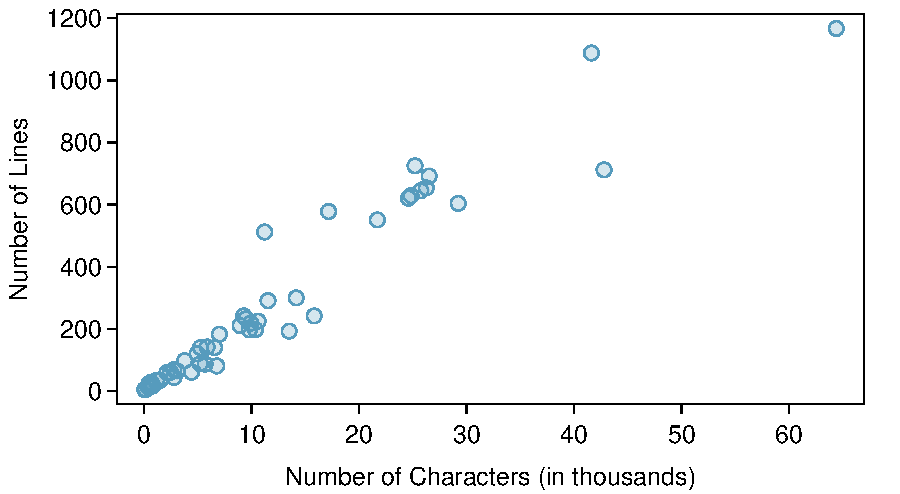
\includegraphics[width=0.75\textwidth]{02/figures/email50LinesCharacters/email50LinesCharacters}
   \caption{A scatterplot of \var{line\_\hspace{0.3mm}breaks} versus \var{num\_\hspace{0.3mm}char} for the \data{email50} data.}
   \label{email50LinesCharacters}
\end{figure}

\textPE{\setlength{\captionwidth}{\mycaptionwidth}}

To put the number of characters in perspective, this paragraph has 363 characters. Looking at Figure~\ref{email50LinesCharacters}, it seems that some emails are incredibly long! Upon further investigation, we would actually find that most of the long emails use the HTML format, which means most of the characters in those emails are used to format the email rather than provide text.

\begin{exercise}
What do scatterplots reveal about the data, and how might they be useful?\footnote{Answers may vary. Scatterplots are helpful in quickly spotting associations between variables, whether those associations represent simple or more complex relationships.}
\end{exercise}

\index{data!cars|(}
\begin{example}{Consider a new data set of 54 cars with two variables: vehicle price and~weight.\footnote{Subset of data from \urlwofont{http://www.amstat.org/publications/jse/v1n1/datasets.lock.html}} A scatterplot of vehicle price versus weight is shown in Figure~\ref{carsPriceVsWeight}. What can be said about the relationship between these variables?}
The relationship is evidently nonlinear, as highlighted by the dashed line. This is different from previous scatterplots we've seen, such as Figure~\vref{county_fed_spendVsPoverty} and Figure~\ref{email50LinesCharacters}, which show relationships that are very linear.

\begin{figure}[h]
   \centering
   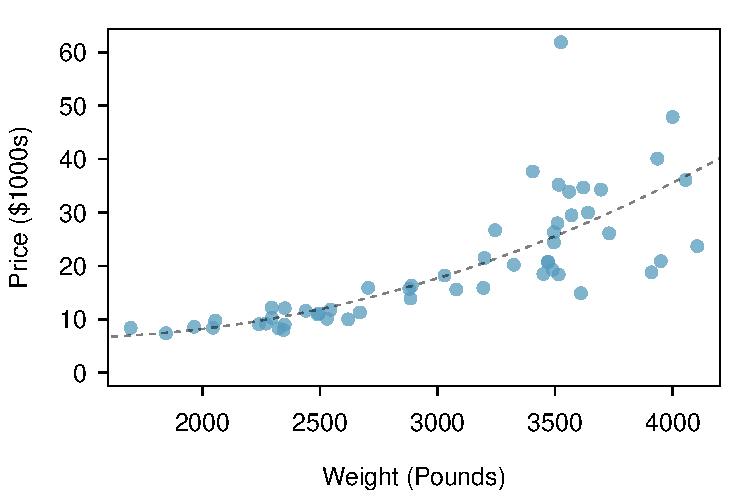
\includegraphics[width=0.65\textwidth]{02/figures/carsPriceVsWeight/carsPriceVsWeight}
   \caption{A scatterplot of \var{price} versus \var{weight} for 54 cars.}
   \label{carsPriceVsWeight}
\end{figure}
\end{example}
\index{data!cars|)}

\begin{exercise}
Describe two variables that would have a horseshoe shaped association in a scatterplot.\footnote{Consider the case where your vertical axis represents something ``good'' and your horizontal axis represents something that is only good in moderation. Health and water consumption fit this description since water becomes toxic when consumed in excessive quantities.}
\end{exercise}

\subsection{Dot plots and the mean}
\label{dotPlot}

Sometimes two variables is one too many: only one variable may be of interest. In these cases, a dot plot provides the most basic of displays. A~\term{dot plot} is a one-variable scatterplot; an example using the number of characters from 50 emails is shown in Figure~\ref{emailCharactersDotPlot}. A stacked version of this dot plot is shown in Figure~\ref{emailCharactersDotPlotStacked}.

\begin{figure}[h]
   \centering
   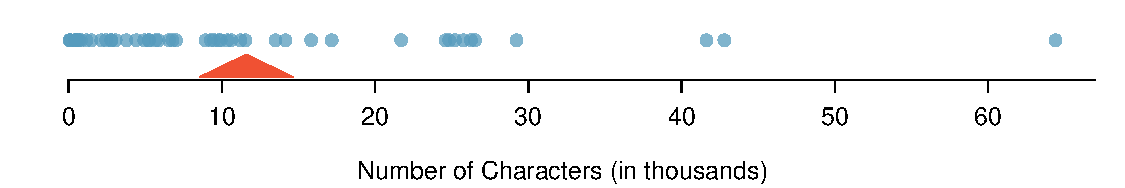
\includegraphics[width=\textwidth]{02/figures/emailCharactersDotPlot/emailCharactersDotPlot}
   \caption{A dot plot of \var{num\_\hspace{0.3mm}char} for the \data{email50} data set.}
   \label{emailCharactersDotPlot}
\end{figure}

\begin{figure}[h]
   \centering
   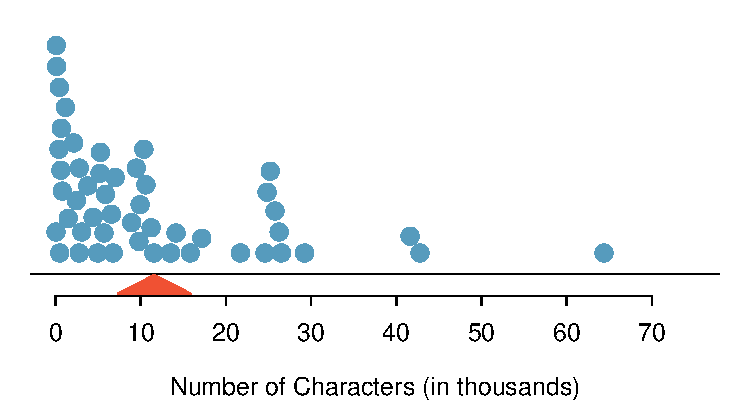
\includegraphics[width=0.67\textwidth]{02/figures/emailCharactersDotPlot/emailCharactersDotPlotStacked}
   \caption{A stacked dot plot of \var{num\_\hspace{0.3mm}char} for the \data{email50} data set.}
   \label{emailCharactersDotPlotStacked}
\end{figure}

The \term{mean}, sometimes called the \indexthis{average}{mean!average}, is a common way to measure the center of a \term{distribution} of data. To find the mean number of characters in the 50 emails, we add up all the character counts and divide by the number of emails. For computational convenience, the number of characters is listed in the thousands and rounded to the first decimal.
\begin{eqnarray}
\bar{x} = \frac{21.7 + 7.0 + \cdots + 15.8}{50} = 11.6
\label{sampleMeanEquation}
\end{eqnarray}
The sample mean is often labeled $\bar{x}$\marginpar[\raggedright$\bar{x}$\\\footnotesize sample\\ mean]{\raggedright$\bar{x}$\\\footnotesize sample\\ mean}, and the letter $x$ is being used as a generic placeholder for the variable of interest, \var{num\_\hspace{0.3mm}char}. The sample mean is shown as a triangle in Figures~\ref{emailCharactersDotPlot} and~\ref{emailCharactersDotPlotStacked}.

\begin{termBox}{\tBoxTitle{Mean}%
The sample mean of a numerical variable is the sum of all of the observations divided by the number of observations:
\begin{eqnarray}
\bar{x} = \frac{x_1+x_2+\cdots+x_n}{n}
\label{meanEquation}
\end{eqnarray}
where $x_1, x_2, \dots, x_n$ represent the $n$ observed values.}
\end{termBox}\marginpar[\raggedright\vspace{-8mm}

$n$\\\footnotesize sample size]{\raggedright\vspace{-8mm}

$n$\\\footnotesize sample size}\vspace{-2mm}

\begin{exercise}
Examine Equations~\eqref{sampleMeanEquation} and~\eqref{meanEquation} above. What does $x_1$ correspond to? And $x_2$? Can you infer a general meaning to what $x_i$ might represent?\footnote{$x_1$ corresponds to the number of characters in the first email in the sample (21.7, in thousands), $x_2$ to the number of characters in the second email (7.0, in thousands), and $x_i$ corresponds to the number of characters in the $i^{th}$ email in the data set.}
\end{exercise}

\begin{exercise}
What was $n$ in this sample of emails?\footnote{The sample size was $n=50$.}
\end{exercise}

The \data{email50} data set is a sample from a larger population of emails that were received in January and March. We could compute a mean for this population in the same way as the sample mean. However, there is a difference in notation: the population mean has a special label: $\mu$\marginpar[\raggedright$\mu$\\\footnotesize population\\ mean]{\raggedright$\mu$\\\footnotesize population\\ mean}. \index{Greek!mu@mu ($\mu$)} The symbol $\mu$ is the Greek letter \emph{mu} and represents the average of all observations in the population. Sometimes a subscript, such as $_x$, is used to represent which variable the population mean refers to, e.g. $\mu_x$.

\begin{example}{The average number of characters across all emails can be estimated using the sample data. Based on the sample of 50 emails, what would be a reasonable estimate of $\mu_x$, the mean number of characters in all emails in the \data{email} data set? (Recall that \data{email50} is a sample from \data{email}.)}
The sample mean, 11,600, may provide a reasonable estimate of $\mu_x$. While this number will not be perfect, it provides a \term{point estimate} of the population mean. In Chapter~\ref{FoundationForInference} and beyond, we will develop tools to characterize the accuracy of point estimates, and we will find that point estimates based on larger samples tend to be more accurate than those based on smaller samples.
\end{example}

\begin{example}{We might like to compute the average income per person in the US. To do so, we might first think to take the mean of the per capita incomes from the 3,143 counties in the \data{county} data set. What would be a better approach?} \label{wtdMeanOfIncome}
The \data{county} data set is special in that each county actually represents many individual people. If we were to simply average across the \var{income} variable, we would be treating counties with 5,000 and 5,000,000 residents equally in the calculations. Instead, we should compute the total income for each county, add up all the counties' totals, and then divide by the number of people in all the counties. If we completed these steps with the \data{county} data, we would find that the per capita income for the US is \$27,348.43. Had we computed the \emph{simple} mean of per capita income across counties, the result would have been just \$22,504.70!
\end{example}

Example~\ref{wtdMeanOfIncome} used what is called a \term{weighted mean}\index{mean!weighted mean}, which will not be a key topic in this textbook. However, we have provided an online supplement on weighted means for interested readers:
\begin{center}
\urlwofont{http://www.openintro.org/stat/down/supp/wtdmean.pdf}
\end{center}

\subsection{Histograms and shape}
\label{histogramsAndShape}

Dot plots show the exact value of each observation. This is useful for small data sets, but they can become hard to read with larger samples. Rather than showing the value of each observation, think of the value as belonging to a \emph{bin}. For example, in the \data{email50} data set, we create a table of counts for the number of cases with character counts between 0 and 5,000, then the number of cases between 5,000 and 10,000, and so on. Observations that fall on the boundary of a bin (e.g. 5,000) are allocated to the lower bin. This tabulation is shown in Table~\ref{binnedNumCharTable}. These binned counts are plotted as bars in Figure~\ref{email50NumCharHist} into what is called a \term{histogram}, which resembles the stacked dot plot shown in Figure~\ref{emailCharactersDotPlotStacked}.

\begin{table}[ht]
\centering\small
\begin{tabular}{l ccc ccc ccc c}
  \hline
Characters & \\
(in thousands) & \raisebox{1.5ex}[0pt]{0-5} & \raisebox{1.5ex}[0pt]{5-10} & \raisebox{1.5ex}[0pt]{10-15} & \raisebox{1.5ex}[0pt]{15-20} & \raisebox{1.5ex}[0pt]{20-25} & \raisebox{1.5ex}[0pt]{25-30} & \raisebox{1.5ex}[0pt]{$\cdots$} & \raisebox{1.5ex}[0pt]{55-60} & \raisebox{1.5ex}[0pt]{60-65} \\
  \hline
Count & 19 & 12 & 6 & 2 & 3 & 5 & $\cdots$ & 0 & 1 \\
  \hline
\end{tabular}
\caption{The counts for the binned \var{num\_\hspace{0.3mm}char} data.}
\label{binnedNumCharTable}
\end{table}

\begin{figure}[bth]
   \centering
   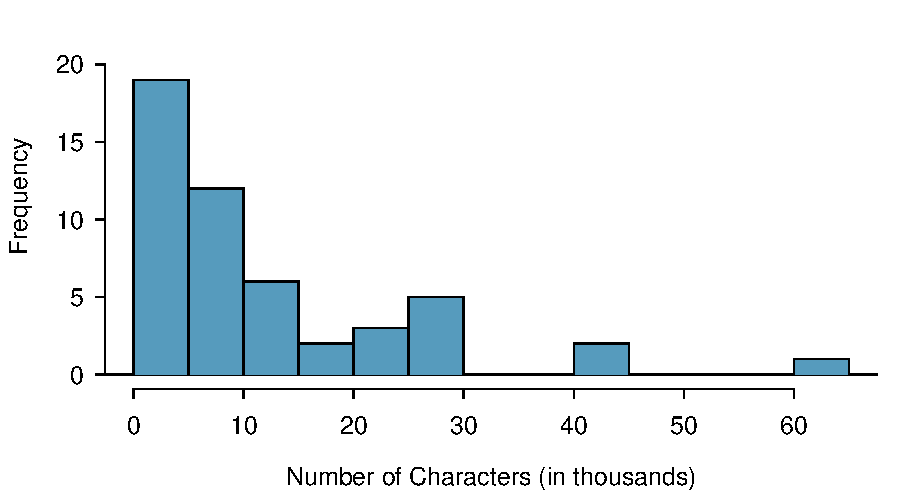
\includegraphics[width=0.82\textwidth]{02/figures/email50NumCharHist/email50NumCharHist}
   \caption{A histogram of \var{num\_\hspace{0.3mm}char}. This distribution is very strongly skewed to the right.\index{skew!example: very strong}}
   \label{email50NumCharHist}
\end{figure}

Histograms provide a view of the \term{data density}. Higher bars represent where the data are relatively more dense. For instance, there are many more emails between 0 and 10,000 characters than emails between 10,000 and 20,000 characters in the data set. The bars make it easy to see how the density of the data changes relative to the number of characters.

Histograms are especially convenient for describing the shape of the data distribution\label{shapeFirstDiscussed}. Figure~\ref{email50NumCharHist} shows that most emails have a relatively small number of characters, while fewer emails have a very large number of characters. When data trail off to the right in this way and have a longer right \hiddenterm{tail}\index{skew!tail}, the shape is said to be \termsub{right skewed}{skew!right skewed}.\footnote{Other ways to describe data that are skewed to the right: \termni{skewed to the right}, \termni{skewed to the high end}, or \termni{skewed to the positive end}.}

Data sets with the reverse characteristic -- a long, thin tail to the left -- are said to be \termsub{left skewed}{skew!left skewed}. We also say that such a distribution has a long left tail. Data sets that show roughly equal trailing off in both directions are called \term{symmetric}.\index{skew!symmetric}

\begin{termBox}{\tBoxTitle{Long tails to identify skew}%
When data trail off in one direction, the distribution has a \term{long tail}. \index{skew!long tail|textbf} If a distribution has a long left tail, it is left skewed. If a distribution has a long right tail, it is right skewed.}
\end{termBox}

\begin{exercise}
Take a look at the dot plots in Figures~\ref{emailCharactersDotPlot} and~\ref{emailCharactersDotPlotStacked}. Can you see the skew in the data? Is it easier to see the skew in this histogram or the dot plots?\footnote{The skew is visible in all three plots, though the flat dot plot is the least useful. The stacked dot plot and histogram are helpful visualizations for identifying skew.}
\end{exercise}

\begin{exercise}
Besides the mean (since it was labeled), what can you see in the dot plots that you cannot see in the histogram?\footnote{Character counts for individual emails.}
\end{exercise}

In addition to looking at whether a distribution is skewed or symmetric, histograms can be used to identify modes. A \term{mode} is represented by a prominent peak in the distribution.\footnote{Another definition of mode, which is not typically used in statistics, is the value with the most occurrences. It is common to have \emph{no} observations with the same value in a data set, which makes this other definition useless for many real data sets.} There is only one prominent peak in the histogram of \var{num\_\hspace{0.3mm}char}.

Figure~\ref{singleBiMultiModalPlots} shows histograms that have one, two, or three prominent peaks. Such distributions are called \termsub{unimodal}{modality!unimodal}, \termsub{bimodal}{modality!bimodal}, and \termsub{multimodal}{modality!multimodal}, respectively. Any distribution with more than 2 prominent peaks is called multimodal. Notice that there was one prominent peak in the unimodal distribution with a second less prominent peak that was not counted since it only differs from its neighboring bins by a few observations.

\begin{figure}[h]
   \centering
   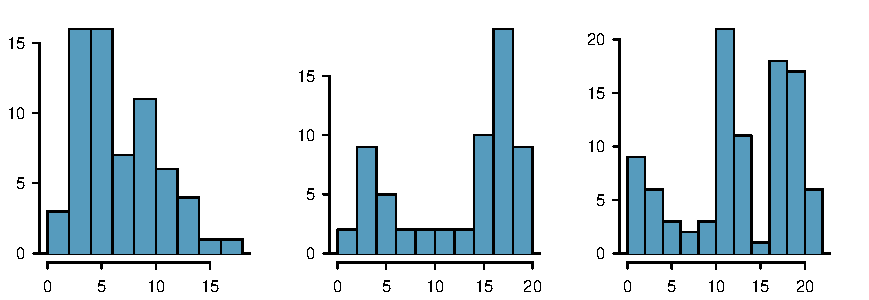
\includegraphics[width=\textwidth]{02/figures/singleBiMultiModalPlots/singleBiMultiModalPlots}
   \caption{Counting only prominent peaks, the distributions are (left to right) unimodal, bimodal, and multimodal.}
   \label{singleBiMultiModalPlots}
\end{figure}

\begin{exercise}
Figure~\ref{email50NumCharHist} reveals only one prominent mode in the number of characters. Is the distribution unimodal, bimodal, or multimodal?\footnote{Unimodal. Remember that \emph{uni} stands for 1 (think \emph{uni}cycles). Similarly, \emph{bi} stands for~2 (think \emph{bi}cycles). (We're hoping a \emph{multicycle} will be invented to complete this analogy.)}
\end{exercise}

\begin{exercise}
Height measurements of young students and adult teachers at a K-3 elementary school were taken. How many modes would you anticipate in this height data set?\footnote{There might be two height groups visible in the data set: one of the students and one of the adults. That is, the data are probably bimodal.}
\end{exercise}

\begin{tipBox}{\tipBoxTitle{Looking for modes}
Looking for modes isn't about finding a clear and correct answer about the number of modes in a distribution, which is why \emph{prominent} is not rigorously defined in this book. The important part of this examination is to better understand your data and how it might be structured.}
\end{tipBox}


\subsection{Variance and standard deviation}
\label{variability}

The mean is used to describe the center of a data set, but the \indexthis{variability}{variability} in the data is also important. Here, we introduce two measures of variability: the variance and the standard deviation. Both of these are very useful in data analysis, even though the formulas are a bit tedious to calculate by hand. The standard deviation is the easier of the two to conceptually understand, and it roughly describes how far away the typical observation is from the mean.

We call the distance of an observation from its mean its \term{deviation}. Below are the deviations for the $1^{st}_{}$, $2^{nd}_{}$, $3^{rd}$, and $50^{th}_{}$ observations in the \var{num\_\hspace{0.3mm}char} variable. For computational convenience, the number of characters is listed in the thousands and rounded to the first decimal.
\begin{align*}
x_1^{}-\bar{x} &= 21.7 - 11.6 = 10.1 \hspace{5mm}\text{ } \\
x_2^{}-\bar{x} &= 7.0 - 11.6 = -4.6 \\
x_3^{}-\bar{x} &= 0.6 - 11.6 = -11.0 \\
			&\ \vdots \\
x_{50}^{}-\bar{x} &= 15.8 - 11.6 = 4.2
\end{align*}
% library(openintro); d <- email50$num_char; round(mean(d),1); d[c(1,2,3,50)]; d[c(1,2,3,50)] - round(mean(d),1); (d[c(1,2,3,50)] - round(mean(d)))^2; sum((d - round(mean(d)))^2)/49; sqrt(sum((d - round(mean(d)))^2)/49); var(d); sd(d)
If we square these deviations and then take an average, the result is about equal to the sample \term{variance}\label{varianceIsDefined}, denoted by $s_{}^2$\marginpar[\raggedright$s^2_{}$\\\footnotesize sample variance]{\raggedright$s^2_{}$\\\footnotesize sample variance}:
\begin{align*}
s_{}^2 &= \frac{10.1_{}^2 + (-4.6)_{}^2 + (-11.0)_{}^2 + \cdots + 4.2_{}^2}{50-1} \\
	&= \frac{102.01 + 21.16 + 121.00 + \cdots + 17.64}{49} \\
	&= 172.44
\end{align*}
We divide by $n-1$, rather than dividing by $n$, when computing the variance; you need not worry about this mathematical nuance for the material in this textbook. Notice that squaring the deviations does two things. First, it makes large values much larger, seen by comparing $10.1^2$, $(-4.6)^2$, $(-11.0)^2$, and $4.2^2$. Second, it gets rid of any negative signs.

The \term{standard deviation} is the square root of the variance:
$$s=\sqrt{172.44} = 13.13$$
\marginpar[\raggedright\vspace{-10mm}

$s$\\\footnotesize sample standard deviation]{\raggedright\vspace{-10mm}

$s$\\\footnotesize sample standard deviation
}\index{s@$s$}The standard deviation of the number of characters in an email is about 13.13 thousand. A subscript of $_x$ may be added to the variance and standard deviation, i.e. $s_x^2$ and $s_x^{}$, as a reminder that these are the variance and standard deviation of the observations represented by $x_1^{}$, $x_2^{}$, ..., $x_n^{}$. The $_{x}$ subscript is usually omitted when it is clear which data the variance or standard deviation is referencing.

\begin{termBox}{\tBoxTitle{Variance and standard deviation}
The variance is roughly the average squared distance from the mean. The standard deviation is the square root of the variance and describes how close the data are to the mean.}
\end{termBox}

Formulas and methods used to compute the variance and standard deviation for a population are similar to those used for a sample.\footnote{The only difference is that the population variance has a division by $n$ instead of $n-1$.} However, like the mean, the population values have special symbols: $\sigma_{}^2$\marginpar[\raggedright$\sigma_{}^2$\\\footnotesize population variance\\ \hspace{2mm}]{\raggedright$\sigma_{}^2$\\\footnotesize population variance\\ \hspace{2mm}} for the variance and $\sigma$\marginpar[\raggedright$\sigma$\\\footnotesize population standard deviation\\ \hspace{2mm}]{\raggedright$\sigma$\\\footnotesize population standard deviation\\ \hspace{2mm}} for the standard deviation. The symbol $\sigma$ \index{Greek!sigma@sigma ($\sigma$)} is the Greek letter \emph{sigma}.


\begin{figure}
\centering
\includegraphics[width=\mycaptionwidth]{02/figures/sdAsRuleForEmailNumChar/sdAsRuleForEmailNumChar}
\caption{In the \var{num\_\hspace{0.3mm}char} data, 41 of the 50 emails (82\%) are within 1~standard deviation of the mean, and 47 of the 50 emails (94\%) are within 2 standard deviations. Usually about 70\% of the data are within 1 standard deviation of the mean and 95\% are within 2 standard deviations, though this rule of thumb is less accurate for skewed data, as shown in this example.}
\label{sdAsRuleForEmailNumChar}
\end{figure}

\begin{tipBox}{\tipBoxTitle{standard deviation describes variability}
Focus on the conceptual meaning of the standard deviation as a descriptor of variability rather than the formulas. Usually 70\% of the data will be within one standard deviation of the mean and about 95\% will be within two standard deviations. However, as seen in Figures~\ref{sdAsRuleForEmailNumChar} and~\ref{severalDiffDistWithSdOf1}, these percentages are not strict rules.}
\end{tipBox}

\begin{figure}
\centering
\includegraphics[width=0.63\textwidth]{02/figures/severalDiffDistWithSdOf1/severalDiffDistWithSdOf1}
\caption{Three very different population distributions with the same mean $\mu=0$ and standard deviation $\sigma=1$.}
\label{severalDiffDistWithSdOf1}
\end{figure}

\begin{exercise}
On page~\pageref{shapeFirstDiscussed}, the concept of shape of a distribution was introduced. A good description of the shape of a distribution should include modality and whether the distribution is symmetric or skewed to one side. Using Figure~\ref{severalDiffDistWithSdOf1} as an example, explain why such a description is important.\footnote{Figure~\ref{severalDiffDistWithSdOf1} shows three distributions that look quite different, but all have the same mean, variance, and standard deviation. Using modality, we can distinguish between the first plot (bimodal) and the last two (unimodal). Using skewness, we can distinguish between the last plot (right skewed) and the first two. While a picture, like a histogram, tells a more complete story, we can use modality and shape (symmetry/skew) to characterize basic information about a~distribution.}
\end{exercise}

\begin{example}{Describe the distribution of the \var{num\_\hspace{0.3mm}char} variable using the histogram in Figure~\vref{email50NumCharHist}. The description should incorporate the center, variability, and shape of the distribution, and it should also be placed in context: the number of characters in emails. Also note any especially unusual cases.}
The distribution of email character counts is unimodal and very strongly skewed to the high end. Many of the counts fall near the mean at 11,600, and most fall within one standard deviation (13,130) of the mean. There is one exceptionally long email with about 65,000 characters.
\end{example}

In practice, the variance and standard deviation are sometimes used as a means to an end, where the ``end'' is being able to accurately estimate the uncertainty associated with a sample statistic. For example, in Chapter~\ref{FoundationForInference} we will use the variance and standard deviation to assess how close the sample mean is to the population mean.

\subsection{Box plots, quartiles, and the median}

A \term{box plot} summarizes a data set using five statistics while also plotting unusual observations. Figure~\ref{boxPlotLayoutNumVar} provides a vertical dot plot alongside a box plot of the \var{num\_\hspace{0.3mm}char} variable from the \data{email50} data set.

\begin{figure}[h]
   \centering
   \includegraphics[width=0.87\mycaptionwidth]{02/figures/boxPlotLayoutNumVar/boxPlotLayoutNumVar}
   \caption{A vertical dot plot next to a labeled box plot for the number of characters in 50 emails. The median (6,890), splits the data into the bottom 50\% and the top 50\%, marked in the dot plot by horizontal dashes and open circles, respectively.}
   \label{boxPlotLayoutNumVar}
\end{figure}

The first step in building a box plot is drawing a dark line denoting the \term{median}, which splits the data in half. Figure~\ref{boxPlotLayoutNumVar} shows 50\% of the data falling below the median (dashes) and other 50\% falling above the median (open circles). There are 50 character counts in the data set (an even number) so the data are perfectly split into two groups of~25. We take the median in this case to be the average of the two observations closest to the $50^{th}$ percentile: $(\text{6,768} + \text{7,012}) / 2 = \text{6,890}$. When there are an odd number of observations, there will be exactly one observation that splits the data into two halves, and in this case that observation is the median (no average needed).

\begin{termBox}{\tBoxTitle{Median: the number in the middle}
If the data are ordered from smallest to largest, the \term{median} is the observation right in the middle. If there are an even number of observations, there will be two values in the middle, and the median is taken as their average.}
\end{termBox}

The second step in building a box plot is drawing a rectangle to represent the middle 50\% of the data. The total length of the box, shown vertically in Figure~\ref{boxPlotLayoutNumVar}, is called the \term{interquartile range} (\hiddenterm{IQR}, for short). It, like the standard deviation, is a measure of \indexthis{variability}{variability} in data. The more variable the data, the larger the standard deviation and~IQR. The two boundaries of the box are called the \term{first quartile} \index{quartile!first quartile} (the $25^{th}$ \hiddenterm{percentile}, i.e. 25\% of the data fall below this value) and the \term{third quartile} \index{quartile!third quartile} (the $75^{th}$ percentile), and these are often labeled $Q_1$ \index{Q$_1$} and $Q_3$\index{Q$_3$}, respectively.

\begin{termBox}{\tBoxTitle{Interquartile range (IQR)}
The IQR\index{interquartile range} is the length of the box in a box plot. It is computed as
\begin{eqnarray*}
IQR = Q_3 - Q_1
\end{eqnarray*}
where $Q_1$ and $Q_3$ are the $25^{th}$ and $75^{th}$ percentiles.}
\end{termBox}

\begin{exercise}
What percent of the data fall between $Q_1$ and the median? What percent is between the median and $Q_3$?\footnote{Since $Q_1$ and $Q_3$ capture the middle 50\% of the data and the median splits the data in the middle, 25\% of the data fall between $Q_1$ and the median, and another 25\% falls between the median and $Q_3$.}
\end{exercise}

Extending out from the box, the \term{whiskers} attempt to capture the data outside of the box, however, their reach is never allowed to be more than $1.5\times IQR$.\footnote{While the choice of exactly 1.5 is arbitrary, it is the most commonly used value for box plots.} They capture everything within this reach. In Figure~\ref{boxPlotLayoutNumVar}, the upper whisker does not extend to the last three points, which are beyond $Q_3 + 1.5\times IQR$, and so it extends only to the last point below this limit. The lower whisker stops at the lowest value, 33, since there is no additional data to reach; the lower whisker's limit is not shown in the figure because the plot does not extend down to $Q_1 - 1.5\times IQR$. In a sense, the box is like the body of the box plot and the whiskers are like its arms trying to reach the rest of the data.

Any observation that lies beyond the whiskers is labeled with a dot. The purpose of labeling these points -- instead of just extending the whiskers to the minimum and maximum observed values -- is to help identify any observations that appear to be unusually distant from the rest of the data. Unusually distant observations are called \termsub{outliers}{outlier}. In this case, it would be reasonable to classify the emails with character counts of 41,623, 42,793, and 64,401 as outliers since they are numerically distant from most of the data.

\begin{termBox}{\tBoxTitle{Outliers are extreme}
An \term{outlier} is an observation that is extreme relative to the rest of the data.}
\end{termBox}


\begin{tipBox}{\tipBoxTitle{Why it is important to look for outliers}
Examination of data for possible outliers serves many useful purposes, including\vspace{-2mm}
\begin{enumerate}
\setlength{\itemsep}{0mm}
\item Identifying \indexthis{strong skew}{skew!strong skew} in the distribution.
\item Identifying data collection or entry errors. For instance, we re-examined the email purported to have 64,401 characters to ensure this value was accurate.
\item Providing insight into interesting properties of the data.\vspace{0.5mm}
\end{enumerate}}
\end{tipBox}

\begin{exercise}
The observation 64,401, an outlier, was found to be an accurate observation. What would such an observation suggest about the nature of character counts in emails?\footnote{That occasionally there may be very long emails.}\end{exercise}

\begin{exercise}
Using Figure~\ref{boxPlotLayoutNumVar}, estimate the following values for \var{num\_\hspace{0.3mm}char} in the \data{email50} data set: (a) $Q_1$, (b) $Q_3$, and (c) IQR.\footnote{These visual estimates will vary a little from one person to the next: $Q_1\approx$ 3,000, $Q_3\approx$ 15,000, $\text{IQR}=Q_3 - Q_1 \approx $ 12,000. (The true values: $Q_1=$ 2,536, $Q_3=$ 15,411, $\text{IQR} = $ 12,875.)}
\end{exercise}

\subsection{Robust statistics}

How are the \indexthis{sample statistics}{sample statistic} of the \data{num\_\hspace{0.3mm}char} data set affected by the observation, 64,401? What would have happened if this email wasn't observed? What would happen to these \indexthis{summary statistics}{summary statistic} if the observation at 64,401 had been even larger, say 150,000? These scenarios are plotted alongside the original data in Figure~\ref{email50NumCharDotPlotRobustEx}, and sample statistics are computed under each scenario in Table~\ref{robustOrNotTable}.

\begin{figure}[ht]
\centering
\includegraphics[width=\textwidth]{02/figures/email50NumCharDotPlotRobustEx/email50NumCharDotPlotRobustEx}
\caption{Dot plots of the original character count data and two modified data sets.}
\label{email50NumCharDotPlotRobustEx}
\end{figure}

\begin{table}[ht]
\centering
\begin{tabular}{l c cc c cc}
  \hline
& \hspace{0mm} & \multicolumn{2}{c}{\bf robust} & \hspace{2mm} & \multicolumn{2}{c}{\bf not robust} \\
scenario && median & IQR && $\bar{x}$ & $s$ \\ 
  \hline
original \var{num\_\hspace{0.3mm}char} data 	&& 6,890 & 12,875 && 11,600 & 13,130 \\
% library(openintro); data(email50); d <- email50$num_char; median(d); diff(quantile(d, c(0.25,0.75))); mean(d); sd(d)
drop 66,924 observation		&& 6,768 & 11,702 && 10,521 & 10,798 \\
% library(openintro); data(email50); d <- email50$num_char; d <- d[-which.max(d)]; median(d); diff(quantile(d, c(0.25,0.75))); mean(d); sd(d)
move 66,924 to 150,000		&& 6,890 & 12,875 && 13,310 & 22,434 \\
% library(openintro); data(email50); d <- email50$num_char; d[which.max(d)] <- 100000; median(d); diff(quantile(d, c(0.25,0.75))); mean(d); sd(d)
   \hline
\end{tabular}
\caption{A comparison of how the median, IQR, mean ($\bar{x}$), and standard deviation ($s$) change when extreme observations are present.}
\label{robustOrNotTable}
\end{table}

\begin{exercise} \label{numCharWhichIsMoreRobust}
(a) Which is more affected by extreme observations, the mean or median? Table~\ref{robustOrNotTable} may be helpful. (b) Is the standard deviation or IQR more affected by extreme observations?\footnote{(a) Mean is affected more. (b) Standard deviation is affected more. Complete explanations are provided in the material following Guided Practice~\ref{numCharWhichIsMoreRobust}.}
\end{exercise}

The median and IQR are called \term{robust estimates} because extreme observations have little effect on their values. The mean and standard deviation are much more affected by changes in extreme observations.

\begin{example}{The median and IQR do not change much under the three scenarios in Table~\ref{robustOrNotTable}. Why might this be the case?}
The median and IQR are only sensitive to numbers near $Q_1$, the median, and $Q_3$. Since values in these regions are relatively stable -- there aren't large jumps between observations -- the median and IQR estimates are also quite stable.
\end{example}

\begin{exercise}
The distribution of vehicle prices tends to be right skewed, with a few luxury and sports cars lingering out into the right tail. If you were searching for a new car and cared about price, should you be more interested in the mean or median price of vehicles sold, assuming you are in the market for a regular car?\footnote{Buyers of a ``regular car'' should be concerned about the median price. High-end car sales can drastically inflate the mean price while the median will be more robust to the influence of those sales.}
\end{exercise}

\subsection{Transforming data (special topic)}
\label{transformingDataSubsection}

When data are very strongly skewed, we sometimes transform them so they are easier to model. Consider the histogram of salaries for Major League Baseball players' salaries from 2010, which is shown in Figure~\ref{histMLBSalariesReg}.

\begin{figure}[ht]
\centering
\subfigure[]{
\includegraphics[width=0.46\textwidth]{02/figures/histMLBSalaries/histMLBSalariesReg}
\label{histMLBSalariesReg}
}
\subfigure[]{
\includegraphics[width=0.46\textwidth]{02/figures/histMLBSalaries/histMLBSalariesLog}
\label{histMLBSalariesLog}
}
\caption{\subref{histMLBSalariesReg} Histogram of MLB player salaries for 2010, in millions of dollars. \subref{histMLBSalariesLog} Histogram of the log-transformed MLB player salaries for 2010.}
\label{histMLBSalaries}
\end{figure}

\begin{example}{The histogram of MLB player salaries is useful in that we can see the data are extremely skewed\index{skew!example: extreme} and centered (as gauged by the median) at about \$1 million. What isn't useful about this plot?}
Most of the data are collected into one bin in the histogram and the data are so strongly skewed that many details in the data are obscured.
\end{example}

There are some standard transformations that are often applied when much of the data cluster near zero (relative to the larger values in the data set) and all observations are positive. A \term{transformation} is a rescaling of the data using a function. For instance, a plot of the natural logarithm\footnote{Statisticians often write the natural logarithm as $\log$. You might be more familiar with it being written as $\ln$.} of player salaries results in a new histogram in Figure~\ref{histMLBSalariesLog}. Transformed data are sometimes easier to work with when applying statistical models because the transformed data are much less skewed and outliers are usually less extreme.

Transformations can also be applied to one or both variables in a scatterplot. A scatterplot of the \var{line\_\hspace{0.3mm}breaks} and \var{num\_\hspace{0.3mm}char} variables is shown in Figure~\ref{email50LinesCharactersMod}, which was earlier shown in Figure~\ref{email50LinesCharacters}. We can see a positive association between the variables and that many observations are clustered near zero. In Chapter~\ref{linRegrForTwoVar}, we might want to use a straight line to model the data. However, we'll find that the data in their current state cannot be modeled very well. Figure~\ref{email50LinesCharactersModLog} shows a scatterplot where both the \var{line\_\hspace{0.3mm}breaks} and \var{num\_\hspace{0.3mm}char} variables have been transformed using a log (base $e$) transformation. While there is a positive association in each plot, the transformed data show a steadier trend, which is easier to model than the untransformed data.

\begin{figure}
\centering
\subfigure[]{
\includegraphics[width=0.46\textwidth]{02/figures/email50LinesCharactersMod/email50LinesCharactersMod}
\label{email50LinesCharactersMod}
}
\subfigure[]{
\includegraphics[width=0.46\textwidth]{02/figures/email50LinesCharactersMod/email50LinesCharactersModLog}
\label{email50LinesCharactersModLog}
}
\caption{\subref{email50LinesCharactersMod} Scatterplot of \var{line\_\hspace{0.3mm}breaks} against \var{num\_\hspace{0.3mm}char} for 50 emails. \subref{email50LinesCharactersModLog} A scatterplot of the same data but where each variable has been log-transformed.}
\label{email50LinesCharactersModMain}
\end{figure}

Transformations other than the logarithm can be useful, too. For instance, the square root ($\sqrt{\text{original observation}}$) and inverse ($\frac{1}{\text{original observation}}$) are used by statisticians. Common goals in transforming data are to see the data structure differently, reduce skew, assist in modeling, or straighten a nonlinear relationship in a scatterplot.

\index{data!email50|)}

\subsection{Mapping data (special topic)}

\index{data!county|(}
\index{intensity map|(}

The \data{county} data set offers many numerical variables that we could plot using dot plots, scatterplots, or box plots, but these miss the true nature of the data. Rather, when we encounter geographic data, we should map it using an \term{intensity map}, where colors are used to show higher and lower values of a variable. Figures~\ref{countyIntensityMaps1} and~\ref{countyIntensityMaps2} shows intensity maps for federal spending per capita (\var{fed\_\hspace{0.3mm}spend}), poverty rate in percent (\var{poverty}), homeownership rate in percent (\var{homeownership}), and median household income (\var{med\_\hspace{0.3mm}income}). The color key indicates which colors correspond to which values. Note that the intensity maps are not generally very helpful for getting precise values in any given county, but they are very helpful for seeing geographic trends and generating interesting research questions.

\begin{figure}
\centering
\subfigure[]{\includegraphics[width=\textwidth]{02/figures/countyIntensityMaps/countyFedSpendMap}\label{countyFedSpendMap}}
\subfigure[]{\includegraphics[width=\textwidth]{02/figures/countyIntensityMaps/countyPovertyMap}\label{countyPovertyMap}}
\caption{\subref{countyFedSpendMap} Map of federal spending (dollars per capita). \subref{countyPovertyMap} Intensity map of poverty rate (percent).}
\label{countyIntensityMaps1}
\end{figure}

\begin{figure}
\centering
\subfigure[]{\includegraphics[width=\textwidth]{02/figures/countyIntensityMaps/countyHomeownershipMap}\label{countyHomeownershipMap}}
\subfigure[]{\includegraphics[width=\textwidth]{02/figures/countyIntensityMaps/countyMedIncomeMap}\label{countyMedIncomeMap}}
\caption{\subref{countyHomeownershipMap} Intensity map of homeownership rate (percent). \subref{countyMedIncomeMap} Intensity map of median household income (\$1000s).}
\label{countyIntensityMaps2}
\end{figure}

\begin{example}{What interesting features are evident in the \var{fed\_\hspace{0.3mm}spend} and \var{poverty} intensity maps?}
The federal spending intensity map shows substantial spending in the Dakotas and along the central-to-western part of the Canadian border, which may be related to the oil boom in this region. There are several other patches of federal spending, such as a vertical strip in eastern Utah and Arizona and the area where Colorado, Nebraska, and Kansas meet. There are also seemingly random counties with very high federal spending relative to their neighbors. If we did not cap the federal spending range at \$18 per capita, we would actually find that some counties have extremely high federal spending while there is almost no federal spending in the neighboring counties. These high-spending counties might contain military bases, companies with large government contracts, or other government facilities with many employees.

Poverty rates are evidently higher in a few locations. Notably, the deep south shows higher poverty rates, as does the southwest border of Texas. The vertical strip of eastern Utah and Arizona, noted above for its higher federal spending, also appears to have higher rates of poverty (though generally little correspondence is seen between the two variables).  High poverty rates are evident in the Mississippi flood plains a little north of New Orleans and also in a large section of Kentucky and West Virginia.
\end{example}

\begin{exercise}
What interesting features are evident in the \var{med\_\hspace{0.3mm}income} intensity map?\footnote{Note: answers will vary. There is a very strong correspondence between high earning and metropolitan areas. You might look for large cities you are familiar with and try to spot them on the map as dark spots.}
\end{exercise}

\index{intensity map|)}
\index{data!county|)}

\subsection{Comparing numerical data across groups}
\label{comparingAcrossGroups}

\index{data!county|(}

Some of the more interesting investigations can be considered by examining numerical data across groups. The methods required here aren't really new. All that is required is to make a numerical plot for each group. Here two convenient methods are introduced: side-by-side box plots and hollow histograms.

We will take a look again at the \data{county} data set and compare the median household income for counties that gained population from 2000 to 2010 versus counties that had no gain. While we might like to make a causal connection here, remember that these are observational data and so such an interpretation would be unjustified.

There were 2,041 counties where the population increased from 2000 to 2010, and there were 1,099 counties with no gain (all but one were a loss). A~random sample of 100 counties from the first group and 50 from the second group are shown in Table~\ref{countyIncomeSplitByPopGainTable} to give a better sense of some of the raw data.

\begin{table}
\centering
\begin{tabular}{ ccc ccc c ccc }
\multicolumn{6}{c}{\bf population gain} && \multicolumn{3}{c}{\bf no gain} \\ 
  \cline{1-6} \cline{8-10}
41.2 & 33.1 & 30.4 & 37.3 & 79.1 & 34.5 &\hspace{5mm}\ & 40.3 & 33.5 & 34.8 \\
22.9 & 39.9 & 31.4 & 45.1 & 50.6 & 59.4 && 29.5 & 31.8 & 41.3 \\
47.9 & 36.4 & 42.2 & 43.2 & 31.8 & 36.9 && 28 & 39.1 & 42.8 \\
50.1 & 27.3 & 37.5 & 53.5 & 26.1 & 57.2 && 38.1 & 39.5 & 22.3 \\
57.4 & 42.6 & 40.6 & 48.8 & 28.1 & 29.4 && 43.3 & 37.5 & 47.1 \\
43.8 & 26 & 33.8 & 35.7 & 38.5 & 42.3 && 43.7 & 36.7 & 36 \\
41.3 & 40.5 & 68.3 & 31 & 46.7 & 30.5 && 35.8 & 38.7 & 39.8 \\
68.3 & 48.3 & 38.7 & 62 & 37.6 & 32.2 && 46 & 42.3 & 48.2 \\
42.6 & 53.6 & 50.7 & 35.1 & 30.6 & 56.8 && 38.6 & 31.9 & 31.1 \\
66.4 & 41.4 & 34.3 & 38.9 & 37.3 & 41.7 && 37.6 & 29.3 & 30.1 \\
51.9 & 83.3 & 46.3 & 48.4 & 40.8 & 42.6 && 57.5 & 32.6 & 31.1 \\
44.5 & 34 & 48.7 & 45.2 & 34.7 & 32.2 && 46.2 & 26.5 & 40.1 \\
39.4 & 38.6 & 40 & 57.3 & 45.2 & 33.1 && 38.4 & 46.7 & 25.9 \\
43.8 & 71.7 & 45.1 & 32.2 & 63.3 & 54.7 && 36.4 & 41.5 & 45.7 \\
71.3 & 36.3 & 36.4 & 41 & 37 & 66.7 && 39.7 & 37 & 37.7 \\
50.2 & 45.8 & 45.7 & 60.2 & 53.1 &  && 21.4 & 29.3 & 50.1 \\
35.8 & 40.4 & 51.5 & 66.4 & 36.1 &  && 43.6 & 39.8 &  \\
\cline{1-6} \cline{8-10}
\end{tabular}
\caption{In this table, median household income (in \$1000s) from a random sample of 100 counties that gained population over 2000-2010 are shown on the left. Median incomes from a random sample of 50 counties that had no population gain are shown on the right.}
\label{countyIncomeSplitByPopGainTable}
\end{table}

The \term{side-by-side box plot} \index{box plot!side-by-side box plot} is a traditional tool for comparing across groups. An example is shown in the left panel of Figure~\ref{countyIncomeSplitByPopGain}, where there are two box plots, one for each group, placed into one plotting window and drawn on the same scale.

\begin{figure}
   \centering
   \includegraphics[width=\textwidth]{02/figures/countyIncomeSplitByPopGain/countyIncomeSplitByPopGain}
   \caption{Side-by-side box plot (left panel) and hollow histograms (right panel) for \var{med\_\hspace{0.3mm}income}, where the counties are split by whether there was a population gain or loss from 2000 to 2010. The income data were collected between 2006 and 2010.}
   \label{countyIncomeSplitByPopGain}
\end{figure}

Another useful plotting method uses \termsub{hollow histograms}{hollow histogram} to compare numerical data across groups. These are just the outlines of histograms of each group put on the same plot, as shown in the right panel of Figure~\ref{countyIncomeSplitByPopGain}.

\begin{exercise} \label{comparingPriceByTypeExercise}
Use the plots in Figure~\ref{countyIncomeSplitByPopGain} to compare the incomes for counties across the two groups. What do you notice about the approximate center of each group? What do you notice about the variability between groups? Is the shape relatively consistent between groups? How many \emph{prominent} modes are there for each group?\footnote{Answers may vary a little. The counties with population gains tend to have higher income (median of about \$45,000) versus counties without a gain (median of about \$40,000). The variability is also slightly larger for the population gain group. This is evident in the IQR, which is about 50\% bigger in the \emph{gain} group. Both distributions show slight to moderate right skew\index{skew!example: slight to moderate} and are unimodal. There is a secondary small bump at about \$60,000 for the \emph{no gain} group, visible in the hollow histogram plot, that seems out of place. (Looking into the data set, we would find that 8 of these 15 counties are in Alaska and Texas.) The box plots indicate there are many observations far above the median in each group, though we should anticipate that many observations will fall beyond the whiskers when using such a large data set.}
\end{exercise}

\begin{exercise}
What components of each plot in Figure~\ref{countyIncomeSplitByPopGain} do you find most useful?\footnote{Answers will vary. The side-by-side box plots are especially useful for comparing centers and spreads, while the hollow histograms are more useful for seeing distribution shape, skew, and groups of anomalies.}
\end{exercise}

\index{data!county|)}


%\section{Exercises}

%_________________
\subsection{Defining probability}

% 1

\eoce{\qt{True or false} Determine if the statements below are true or false, and explain your reasoning.
\begin{parts}
\item If a fair coin is tossed many times and the last eight tosses are all heads, then the chance that the next toss will be heads is somewhat less than 50\%.
\item Drawing a face card (jack, queen, or king) and drawing a red card from a full deck of playing cards are mutually exclusive events.
\item Drawing a face card and drawing an ace from a full deck of playing cards are mutually exclusive events.
\end{parts}
}{}

% 2

\eoce{\qt{Roulette wheel\label{roulette_wheel}} The game of roulette involves spinning a wheel with 38 slots: 18 red, 18 black, and 2 green. A ball is spun onto the wheel and will eventually land in a slot, where each slot has an equal chance of capturing the ball. \footfullcite{rouletteWheelPic}

\noindent\begin{minipage}[c]{0.725\textwidth}
\begin{parts}
\item You watch a roulette wheel spin 3 consecutive times and the ball lands on a red slot each time. What is the probability that the ball will land on a red slot on the next spin?
\item You watch a roulette wheel spin 300 consecutive times and the ball lands on a red slot each time. What is the probability that the ball will land on a red slot on the next spin?
\item Are you equally confident of your answers to parts~(a) and~(b)? Why or why not?
\end{parts}
\end{minipage}
\begin{minipage}[c]{0.025\textwidth}
\end{minipage}
\begin{minipage}[c]{0.25\textwidth}
\hfill\includegraphics[width = 0.94\textwidth]{02/figures/eoce/images/roulette_wheel}
\end{minipage}
}{}


% 3

\eoce{\qt{Four games, one winner} Below are four versions of the same game. Your archnemisis gets to pick the version of the game, and then you get to choose how many times to flip a coin: 10 times or 100 times. Identify how many coin flips you should choose for each version of the game. Explain your reasoning.
\begin{parts}
\item If the proportion of heads is larger than 0.60, you win \$1.
\item If the proportion of heads is larger than 0.40, you win \$1.
\item If the proportion of heads is between 0.40 and 0.60, you win \$1.
\item If the proportion of heads is smaller than 0.30, you win \$1.
\end{parts}
}{}

% 4

\eoce{\qt{Backgammon} Backgammon is a board game for two players in which the playing pieces are moved according to the roll of two dice. Players win by removing all of their pieces from the board, so it is usually good to roll high numbers. You are playing backgammon with a friend and you roll two 6s in your first roll and two 6s in your second roll. Your friend rolls two 3s in his first roll and again in his second row. Your friend claims that you are cheating, because rolling double 6s twice in a row is very unlikely. Using probability, show that your rolls were just as likely as his.
}{}

% 5

\eoce{\qt{Coin flips} If you flip a fair coin 10 times, what is the probability of \vspace{-3mm}
\begin{multicols}{3}
\begin{parts}
\item getting all tails? 
\item getting all heads? 
\item getting at least one tails? 
\end{parts}
\end{multicols}
}{}

% 6

\eoce{\qt{Dice rolls} If you roll a pair of fair dice, what is the probability of \textB{\vspace{-3mm}}
\begin{multicols}{3}
\begin{parts}
\item getting a sum of 1?
\item getting a sum of 5?
\item getting a sum of 12?
\end{parts}
\end{multicols} 
}{}

% 7
\textB{\pagebreak}

\eoce{\qt{Swing voters\label{indepSwing}} A 2012 Pew Research survey asked 2,373 randomly sampled registered voters their political affiliation (Republican, Democrat, or Independent) and whether or not they identify as swing voters. 35\% of respondents identified as Independent, 23\% identified as swing voters, and 11\% identified as both.\footfullcite{indepSwing}
\begin{parts}
\item Are being Independent and being a swing voter disjoint, i.e. mutually exclusive?
\item Draw a Venn diagram summarizing the variables and their associated probabilities.
\item What percent of voters are Independent but not swing voters?
\item What percent of voters are Independent or swing voters?
\item What percent of voters are neither Independent nor swing voters?
\item Is the event that someone is a swing voter independent of the event that someone is a political Independent?
\end{parts}
}{}

% 8

\eoce{\qt{Poverty and language\label{poorLang}} The American Community Survey is an ongoing survey that provides data every year to give communities the current information they need to plan investments and services. The 2010 American Community Survey estimates that 14.6\% of Americans live below the poverty line, 20.7\% speak a language other that English at home, and 4.2\% fall into both categories. \footfullcite{poorLang}
\begin{parts}
\item Are living below the poverty line and speaking a language other than English at home disjoint?
\item Draw a Venn diagram summarizing the variables and their associated probabilities.
\item What percent of Americans live below the poverty line and only speak English at home?
\item What percent of Americans live below the poverty line or speak a language other than English at home?
\item What percent of Americans live above the poverty line and only speak English at home? 
\item Is the event that someone lives below the poverty line independent of the event that the person speaks a language other than English at home?
\end{parts}
}{}

% 9

\eoce{\qt{Disjoint vs. independent} In parts~(a) and~(b), identify whether the events are disjoint, independent, or neither (events cannot be both disjoint and independent).
\begin{parts}
\item You and a randomly selected student from your class both earn A's in this course. 
\item You and your class study partner both earn A's in this course.
\item If two events can occur at the same time, must they be dependent?
\end{parts}
}{}

% 10

\eoce{\qt{Guessing on an exam} In a multiple choice exam, there are 5 questions and 4 choices for each question (a, b, c, d). Nancy has not studied for the exam at all and decides to randomly guess the answers. What is the probability that:
\begin{parts}
\item the first question she gets right is the $5^{th}$ question?
\item she gets all of the questions right?
\item she gets at least one question right?
\end{parts}
}{}

% 11
\textB{\pagebreak}

\eoce{\qt{Educational attainment of couples} The table below shows the distribution of education level attained by US residents by gender based on data collected during the 2010 American Community Survey.\footfullcite{eduSex}
\begin{center}
\begin{tabular}{l p{7cm} c c }
&						& \multicolumn{2}{c}{\textit{Gender}} \\
\cline{3-4}
&												& Male	& Female \\
\cline{2-4}
& Less than 9th grade								&0.07	&0.13	 \\
& 9th to 12th grade, no diploma						&0.10	&0.09	 \\
\textit{Highest} & High school graduate, GED, or alternative	&0.30	&0.20	 \\
\textit{education} & Some college, no degree				&0.22	&0.24	 \\ 
\textit{attained} & Associate's degree					&0.06	&0.08	 \\
& Bachelor's degree									&0.16	&0.17	 \\
& Graduate or professional degree						&0.09	&0.09	 \\
\cline{2-4}
& Total											& 1.00	& 1.00
\end{tabular}
\end{center}
\begin{parts}
\item What is the probability that a randomly chosen man has at least a Bachelor's degree?
\item What is the probability that a randomly chosen woman has at least a Bachelor's degree?
\item What is the probability that a man and a woman getting married both have at least a Bachelor's degree? Note any assumptions you must make to answer this question.
\item If you made an assumption in part~(c), do you think it was reasonable? If you didn't make an assumption, double check your earlier answer and then return to this part.
\end{parts}
}{}

% 12

\eoce{\qt{School absences\label{elementarySchoolSick}} Data collected at elementary schools in DeKalb County, GA suggest that each year roughly 25\% of students miss exactly one day of school, 15\% miss 2 days, and 28\% miss 3 or more days due to sickness. \footfullcite{Mizan:2011}
\begin{parts}
\item What is the probability that a student chosen at random doesn't miss any days of school due to sickness this year?
\item What is the probability that a student chosen at random misses no more than one day?
\item What is the probability that a student chosen at random misses at least one day?
\item If a parent has two kids at a DeKalb County elementary school, what is the probability that neither kid will miss any school? Note any assumption you must make to answer this question.
\item If a parent has two kids at a DeKalb County elementary school, what is the probability that that both kids will miss some school, i.e. at least one day? Note any assumption you make.
\item If you made an assumption in part~(d) or~(e), do you think it was reasonable? If you didn't make any assumptions, double check your earlier answers.
\end{parts}
}{}

% 13

\eoce{\qt{Grade distributions} Each row in the table below is a proposed grade distribution for a class. Identify each as a valid or invalid probability distribution, and explain your reasoning.
\begin{center}
\begin{tabular}{l  ccccc} 
	& \multicolumn{5}{c}{\textit{Grades}} \\
\cline{2-6}
	& A		& B 		& C 		& D		& F  \\
\cline{2-6}
(a) 	& 0.3 	& 0.3 	& 0.3 	& 0.2 	& 0.1\\
(b) 	& 0	 	& 0	 	& 1		& 0		& 0 \\
(c) 	& 0.3 	& 0.3 	& 0.3		& 0		& 0 \\
(d) 	& 0.3 	& 0.5 	& 0.2		& 0.1		& -0.1 \\
(e) 	& 0.2 	& 0.4 	& 0.2		& 0.1		& 0.1 \\
(f) 	& 0	 	& -0.1 	& 1.1		& 0		& 0 \\
\end{tabular}
\end{center}
}{}

% 14
\textB{\pagebreak}

\eoce{\qt{Weight and health coverage, Part I\label{healthCovBMI}} The Behavioral Risk Factor Surveillance System (BRFSS) is an annual telephone survey designed to identify risk factors in the adult population and report emerging health trends. The following table summarizes two variables for the respondents: weight status using body mass index (BMI) and health coverage, which describes whether each respondent had health insurance. \footfullcite{data:BRFSS2010}

\begin{center}
\begin{tabular}{ll  ccc  c} 
			&	\multicolumn{1}{c}{}	& \multicolumn{3}{c}{\textit{Weight Status}} & \\ 
\cline{3-5}
			&		& Neither overweight 	& Overweight 	& Obese	&   \\
			&		& nor obese (BMI $<$ 25)&(25 $\le$ BMI $<$ 30) & (BMI $\ge$ 30) & Total \\
\cline{2-6}
\textit{Health}	&Yes 	& 134,801 	& 141,699 	& 107,301 		& 383,801\\
\textit{Coverage}&No 	& 15,098 		& 15,327 		& 14,412			& 44,837 \\
\cline{2-6}
			&Total	& 149,899		&157,026		& 121,713			& 428,638
\end{tabular}
\end{center}

\begin{parts}
\item If we draw one individual at random, what is the probability that the respondent is overweight and doesn't have health coverage?
\item If we draw one individual at random, what is the probability that the respondent is overweight or doesn't have health coverage?
\end{parts}
}{}


%_________________
\subsection{Conditional probability}

% 15

\eoce{\qt{Joint and conditional probabilities} P(A) = 0.3, P(B) = 0.7
\begin{parts}
\item Can you compute P(A and B) if you only know P(A) and P(B)?
\item Assuming that events A and B arise from independent random processes,
\begin{subparts}
\item what is P(A and B)?
\item what is P(A or B)?
\item what is P(A$|$B)?
\end{subparts}
\item If we are given that P(A and B) = 0.1, are the random variables giving rise to events A and B independent?
\item If we are given that P(A and B) = 0.1, what is P(A$|$B)?
\end{parts}
}{}

% 16

\eoce{\qt{PB \& J} Suppose 80\% of people like peanut butter, 89\% like jelly, and 78\% like both. Given that a randomly sampled person likes peanut butter, what's the probability that he also likes jelly?
}{}

% 17

\eoce{\qt{Global warming} A 2010 Pew Research poll asked 1,306 Americans ``From what you've read and heard, is there solid evidence that the average temperature on earth has been getting warmer over the past few decades, or not?". The table below shows the distribution of responses by party and ideology, where the counts have been replaced with relative frequencies.\footfullcite{globalWarming}
\begin{center}
\begin{tabular}{ll  ccc c} 
							&			& \multicolumn{3}{c}{\textit{Response}} \\
\cline{3-5}
							&			& Earth is 		& Not 		& Don't Know	&	\\
							&			& warming	& warming 	& Refuse		& Total\\
\cline{2-6}
				& Conservative Republican	& 0.11	 	& 0.20		& 0.02 		& 0.33 	\\
\textit{Party and}	& Mod/Lib Republican		& 0.06	 	& 0.06 	 	& 0.01		& 0.13 \\
\textit{Ideology}		& Mod/Cons Democrat		& 0.25	 	& 0.07 	 	& 0.02 		& 0.34 \\
				& Liberal Democrat			& 0.18	 	& 0.01 	 	& 0.01 		& 0.20\\
\cline{2-6}
							&Total		& 0.60		& 0.34		& 0.06		& 1.00
\end{tabular}
\end{center}
\begin{parts}
\item What is the probability that a randomly chosen respondent believes the earth is warming or is a liberal Democrat?
\item What is the probability that a randomly chosen respondent believes the earth is warming given that he is a liberal Democrat?
\item What is the probability that a randomly chosen respondent believes the earth is warming given that he is a conservative Republican?
\item Does it appear that whether or not a respondent believes the earth is warming is independent of their party and ideology? Explain your reasoning.
\item What is the probability that a randomly chosen respondent is a moderate/liberal Republican given that he does not believe that the earth is warming? 
\end{parts}
}{}

% 18

\eoce{\qt{Weight and health coverage, Part II} Exercise~\ref{healthCovBMI} introduced a contingency table summarizing the relationship between weight status, which is determined based on body mass index (BMI), and health coverage for a sample of 428,638 Americans. In the table below, the counts have been replaced by relative frequencies (probability estimates).

\begin{center}
\begin{tabular}{ll  ccc  c} 
			&	\multicolumn{1}{c}{}	& \multicolumn{3}{c}{\textit{Weight Status}} & \\ 
\cline{3-5}
			&		& Neither overweight 	& Overweight 	& Obese	&   \\
			&		& nor obese (BMI $<$ 25)&(25 $\le$ BMI $<$ 30) & (BMI $\ge$ 30) & Total \\
\cline{2-6}
\textit{Health}	&Yes 	& 0.3145	 	& 0.3306	 	& 0.2503	 		& 0.8954\\
\textit{Coverage}&No 	& 0.0352 		& 0.0358 		& 0.0336			& 0.1046 \\
\cline{2-6}
			&Total	& 0.3497		&0.3664		& 0.2839			& 1.0000
\end{tabular}
\end{center}

\begin{parts}
\item What is the probability that a randomly chosen individual is obese?
\item What is the probability that a randomly chosen individual is obese given that he has health coverage?
\item What is the probability that a randomly chosen individual is obese given that he doesn't have health coverage?
\item Do being overweight and having health coverage appear to be independent?
\end{parts}
}{}

% 19

\eoce{\qt{Burger preferences} A 2010 SurveyUSA poll asked 500 Los Angeles residents, ``What is the best hamburger place in Southern California? Five Guys Burgers? In-N-Out Burger? Fat Burger? Tommy's Hamburgers? Umami Burger? Or somewhere else?'' The distribution of responses by gender is shown below. \footfullcite{burgers}
\begin{center}
\begin{tabular}{l p{4cm} r r r }
&						& \multicolumn{2}{c}{\textit{Gender}} \\
\cline{3-4}
&								& Male	& Female 	& Total\\
\cline{2-5}
& Five Guys Burgers					&5		&6	 	& 11	\\
& In-N-Out Burger					&162	&181	& 343 \\
\textit{Best} & Fat Burger				&10		&12	 	& 22 \\
\textit{hamburger} & Tommy's Hamburgers	&27		&27	 	& 54	\\ 
\textit{place} & Umami Burger			&5		&1	 	& 6 \\
& Other							&26		&20	 	& 46 \\
& Not Sure						&13		&5	 	& 18 \\
\cline{2-5}
&Total							&248	&252	& 500
\end{tabular}
\end{center}
\begin{parts}
\item What is the probability that a randomly chosen male likes In-N-Out the best?
\item What is the probability that a randomly chosen female likes In-N-Out the best?
\item What is the probability that a man and a woman who are dating both like In-N-Out the best? Note any assumption you make and evaluate whether you think that assumption is reasonable.
\item What is the probability that a randomly chosen person likes Umami best or that person is female?
\end{parts}
}{}

% 20

\eoce{\qt{Assortative mating} Assortative mating is a nonrandom mating pattern where individuals with similar genotypes and/or phenotypes mate with one another more frequently than what would be expected under a random mating pattern. Researchers studying this topic collected data on eye colors of  204 Scandinavian men and their female partners. The table below summarizes the results. For simplicity, we only include heterosexual relationships in this exercise. \footfullcite{Laeng:2007}
\begin{center}
\begin{tabular}{ll  ccc c} 
							&			& \multicolumn{3}{c}{\textit{Partner (female)}} \\
\cline{3-5}
							&			& Blue 	& Brown	& Green 	& Total	\\
\cline{2-6}
							&Blue 		& 78	 	& 23		& 13		& 114 	\\
\multirow{2}{*}{\textit{Self (male)}}	&Brown		& 19	 	& 23 	 	& 12		& 54 \\
							&Green		& 11	 	& 9 	 	& 16		& 36 \\
\cline{2-6}	
							&Total		& 108	& 55		& 41		& 204
\end{tabular}
\end{center}
\begin{parts}
\item What is the probability that a randomly chosen male respondent or his partner has blue eyes?
\item What is the probability that a randomly chosen male respondent with blue eyes has a partner with blue eyes? 
\item What is the probability that a randomly chosen male respondent with brown eyes has a partner with blue eyes? What about the probability of a randomly chosen male respondent with green eyes having a partner with blue eyes?
\item Does it appear that the eye colors of male respondents and their partners are independent? Explain your reasoning.
\end{parts}
}{}

% 21

\eoce{\qt{Drawing box plots\label{constructingBoxPlots}} After an introductory statistics course, 80\% of students can successfully construct box plots. Of those who can construct box plots, 86\% passed, while only 65\% of those students who could not construct box plots passed.
\begin{parts}
\item Construct a tree diagram of this scenario.
\item Calculate the probability that a student is able to construct a box plot if it is known that he passed.
\end{parts}
}{}

% 22

\eoce{\qt{Predisposition for thrombosis} A genetic test is used to determine if people have a predisposition for \textit{thrombosis}, which is the formation of a blood clot inside a blood vessel that obstructs the flow of blood through the circulatory system. It is believed that 3\% of people actually have this predisposition. The genetic test is 99\% accurate if a person actually has the predisposition, meaning that the probability of a positive test result when a person actually has the predisposition is 0.99. The test is 98\% accurate if a person does not have the predisposition. What is the probability that a randomly selected person who tests positive for the predisposition by the test actually has the predisposition?
}{}

% 23

\eoce{\qt{HIV in Swaziland} Swaziland has the highest HIV prevalence in the world: 25.9\% of this country's population is infected with HIV.\footfullcite{ciaFactBookHIV:2012} The ELISA test is one of the first and most accurate tests for HIV. For those who carry HIV, the ELISA test is 99.7\% accurate. For those who do not carry HIV, the test is 92.6\% accurate. If an individual from Swaziland has tested positive, what is the probability that he carries HIV?
}{}

% 24

\eoce{\qt{Exit poll} Edison Research gathered exit poll results from several sources for the Wisconsin recall election of Scott Walker. They found that 53\% of the respondents voted in favor of Scott Walker. Additionally, they estimated that of those who did vote in favor for Scott Walker, 37\% had a college degree, while 44\% of those who voted against Scott Walker had a college degree. Suppose we randomly sampled a person who participated in the exit poll and found that he had a college degree. What is the probability that he voted in favor of Scott Walker?\footfullcite{data:scott}
}{}

% 25

\eoce{\qt{It's never lupus} Lupus is a medical phenomenon where antibodies that are supposed to attack foreign cells to prevent infections instead see plasma proteins as foreign bodies, leading to a high risk of blood clotting. It is believed that 2\% of the population suffer from this disease. The test is 98\% accurate if a person actually has the disease. The test is 74\% accurate if a person does not have the disease. 

There is a line from the Fox television show \emph{House} that is often used after a patient tests positive for lupus: ``It's never lupus." Do you think there is truth to this statement? Use appropriate probabilities to support your answer.
}{}

% 26

\eoce{\qt{Twins} About 30\% of human twins are identical, and the rest are fraternal. Identical twins are necessarily the same sex -- half are males and the other half are females. One-quarter of fraternal twins are both male, one-quarter both female, and one-half are mixes: one male, one female. You have just become a parent of twins and are told they are both girls. Given this information, what is the probability that they are identical?
}{}


%_________________
\subsection{Sampling from a small population}

% 27

\eoce{\qt{Urns and marbles, Part I\label{urnWithMarbles}} Imagine you have an urn containing 5 red, 3 blue, and 2 orange marbles in it. 
\begin{parts}
\item What is the probability that the first marble you draw is blue?
\item Suppose you drew a blue marble in the first draw. If drawing with replacement, what is the probability of drawing a blue marble in the second draw?
\item Suppose you instead drew an orange marble in the first draw. If drawing with replacement, what is the probability of drawing a blue marble in the second draw?
\item If drawing with replacement, what is the probability of drawing two blue marbles in a row?
\item When drawing with replacement, are the draws independent? Explain.
\end{parts}
}{}

% 28

\eoce{\qt{Socks in a drawer} In your sock drawer you have 4 blue, 5 gray, and 3 black socks. Half asleep one morning you grab 2 socks at random and put them on. Find the probability you end up wearing
\begin{parts}
\item 2 blue socks
\item no gray socks
\item at least 1 black sock
\item a green sock
\item matching socks
\end{parts}
}{}


% 29

\eoce{\qt{Urns and marbles, Part II} Imagine you have an urn containing 5 red, 3 blue, and 2 orange marbles.
\begin{parts}
\item Suppose you draw a marble and it is blue. If drawing without replacement, what is the probability the next is also blue?
\item Suppose you draw a marble and it is orange, and then you draw a second marble without replacement. What is the probability this second marble is blue?
\item If drawing without replacement, what is the probability of drawing two blue marbles in a row?
\item When drawing without replacement, are the draws independent? Explain.
\end{parts}
}{}

% 30
\textB{\pagebreak}

\eoce{\qt{Books on a bookshelf} The table below shows the distribution of books on a bookcase based on whether they are nonfiction or fiction and hardcover or paperback. \vspace{-2.5mm}
\begin{center}
\begin{tabular}{ll  cc c} 
							&			& \multicolumn{2}{c}{\textit{Format}} \\
\cline{3-4}
							&			& Hardcover 	& Paperback 	& Total	\\
\cline{2-5}
\multirow{2}{*}{\textit{Type}}		&Fiction 		& 13	 		& 59			& 72 	\\
							&Nonfiction	& 15	 		& 8 	 		& 23 \\
\cline{2-5}	
							&Total		& 28			& 67			& 95 \\
\cline{2-5}
\end{tabular}
\end{center} \vspace{-2.5mm}
\begin{parts}
\item Find the probability of drawing a hardcover book first then a paperback fiction book second when drawing without replacement.
\item Determine the probability of drawing a fiction book first and then a hardcover book second, when drawing without replacement.
\item Calculate the probability of the scenario in part~(b), except this time complete the calculations under the scenario where the first book is placed back on the bookcase before randomly drawing the second book.
\item The final answers to parts~(b) and~(c) are very similar. Explain why this is the case.
\end{parts}
}{}

% 31

\eoce{\qt{Student outfits} In a classroom with 24 students, 7 students are wearing jeans, 4 are wearing shorts, 8 are wearing skirts, and the rest are wearing leggings. If we randomly select 3 students without replacement, what is the probability that one of the selected students is wearing leggings and the other two are wearing jeans? Note that these are mutually exclusive clothing options.
}{}

% 32

\eoce{\qt{The birthday problem} Suppose we pick three people at random. For each of the following questions, ignore the special case where someone might be born on February 29th, and assume that births are evenly distributed throughout the year.
\begin{parts}
\item What is the probability that the first two people share a birthday? 
\item What is the probability that at least two people share a birthday?
\end{parts}
}{}


%_________________
\subsection{Random variables}

% 33

\eoce{\qt{College smokers} At a university, 13\% of students smoke.
\begin{parts}
\item Calculate the expected number of smokers in a random sample of 100 students from this university.
\item The university gym opens at 9am on Saturday mornings. One Saturday morning at 8:55am there are 27 students outside the gym waiting for it to open. Should you use the same approach from part (a) to calculate the expected number of smokers among these 27 students?
\end{parts}
}{}

% 34

\eoce{\qt{Card game} Consider the following card game with a well-shuffled deck of cards. If you draw a red card, you win nothing. If you get a spade, you win \$5. For any club, you win \$10 plus an extra \$20 for the ace of clubs.
\begin{parts}
\item Create a probability model for the amount you win at this game. Also, find the expected winnings for a single game and the standard deviation of the winnings.
\item What is the maximum amount you would be willing to pay to play this game? Explain.
\end{parts}
}{}

% 35

\eoce{\qt{Another card game} In a new card game, you start with a well-shuffled full deck and draw 3 cards without replacement. If you draw 3 hearts, you win \$50. If you draw 3 black cards, you win \$25. For any other draws, you win nothing.
\begin{parts}
\item Create a probability model for the amount you win at this game, and find the expected winnings. Also compute the standard deviation of this distribution.
\item If the game costs \$5 to play, what would be the expected value and standard deviation of the net profit (or loss)? \textit{(Hint: profit = winnings $-$ cost; $X-5$)}
\item If the game costs \$5 to play, should you play this game? Explain.
\end{parts}
}{}

% 36

\eoce{\qtq{Is it worth it} Andy is always looking for ways to make money fast. Lately, he has been trying to make money by gambling. Here is the game he is considering playing: The game costs \$2 to play. He draws a card from a deck. If he gets a number card (2-10), he wins nothing. For any face card (jack, queen or king), he wins \$3. For any ace, he wins \$5, and he wins an \textit{extra} \$20 if he draws the ace of clubs.
\begin{parts}
\item Create a probability model and find Andy's expected profit per game.
\item Would you recommend this game to Andy as a good way to make money? Explain.
\end{parts}
}{}

% 37

\eoce{\qt{Portfolio return} A portfolio's value increases by 18\% during a financial boom and by 9\% during normal times. It decreases by 12\% during a recession. What is the expected return on this portfolio if each scenario is equally likely?
}{}

% 38

\eoce{\qt{A game of roulette, Part I\label{roulette}} The game of roulette involves spinning a wheel with 38 slots: 18 red, 18 black, and 2 green. A ball is spun onto the wheel and will eventually land in a slot, where each slot has an equal chance of capturing the ball. Gamblers can place bets on red or black. If the ball lands on their color, they double their money. If it lands on another color, they lose their money. Suppose you bet \$1 on red. What's the expected value and standard deviation of your winnings?
}{}

% 39

\eoce{\qt{A game of roulette, Part II} Exercise~\ref{roulette} describes winnings on a game of roulette.
\begin{parts}
\item Suppose you play roulette and bet \$3 on a single round. What is the expected value and standard deviation of your total winnings?
\item Suppose you bet \$1 in three different rounds. What is the expected value and standard deviation of your total winnings?
\item How do your answers to parts (a) and (b) compare? What does this say about the riskiness of the two games?
\end{parts}
}{}

% 40

\eoce{\qt{Baggage fees\label{americanAir}} An airline charges the following baggage fees: \$25 for the first bag and \$35 for the second. Suppose 54\% of passengers have no checked luggage, 34\% have one piece of checked luggage and 12\% have two pieces. We suppose a negligible portion of people check more than two bags.
\begin{parts}
\item Build a probability model, compute the average revenue per passenger, and compute the corresponding standard deviation.
\item About how much revenue should the airline expect for a flight of 120 passengers? With what standard deviation? Note any assumptions you make and if you think they are justified.
\end{parts}
}{}

% 41

\eoce{\qt{Dodgers vs. Padres} You and your friend decide to bet on the Major League Baseball game happening one evening between the Los Angeles Dodgers and the San Diego Padres. Suppose current statistics indicate that the Dodgers have a 0.46 probability of winning this game against the Padres. If your friend bets you \$5 that the Dodgers will win, how much would you need to bet on the Padres to make this a fair game?
}{}

% 42

\eoce{\qt{Selling on Ebay} Marcie has been tracking the following two items on Ebay:
\begin{itemize}
\item A textbook that sells for an average of \$110 with a standard deviation of \$4.
\item Mario Kart for the Nintendo Wii, which sells for an average of \$38 with a standard deviation of \$5.
\end{itemize}
\begin{parts}
\item Marcie wants to sell the video game and buy the textbook. How much net money (profits - losses) would she expect to make or spend? Also compute the standard deviation of how much she would make or spend.
\item Lucy is selling the textbook on Ebay for a friend, and her friend is giving her a 10\% commission (Lucy keeps 10\% of the revenue). How much money should she expect to make? With what standard deviation?
\end{parts}
}{}

% 43

\eoce{\qt{Cost of breakfast} Sally gets a cup of coffee and a muffin every day for breakfast from one of the many coffee shops in her neighborhood. She picks a coffee shop each morning at random and independently of previous days. The average price of a cup of coffee is \$1.40 with a standard deviation of 30\textcent (\$0.30), the average price of a muffin is \$2.50 with a standard deviation of 15\textcent, and the two prices are independent of each other.
\begin{parts}
\item What is the mean and standard deviation of the amount she spends on breakfast daily?
\item What is the mean and standard deviation of the amount she spends on breakfast weekly (7~days)?
\end{parts}
}{}

% 44

\eoce{\qt{Ice cream} Ice cream usually comes in 1.5 quart boxes (48 fluid ounces), and ice cream scoops hold about 2 ounces. However, there is some variability in the amount of ice cream in a box as well as the amount of ice cream scooped out. We represent the amount of ice cream in the box as $X$ and the amount scooped out as $Y$. Suppose these random variables have the following means, standard deviations, and variances:
\begin{center}
\begin{tabular}{l ccc}
\hline
	& mean & SD & variance \\
\hline
$X$	& 48	   & 1		& 1		\\
$Y$ & 2	   & 0.25	& 0.0625	\\
\hline
\end{tabular}
\end{center}
\begin{parts}
\item An entire box of ice cream, plus 3 scoops from a second box is served at a party. How much ice cream do you expect to have been served at this party? What is the standard deviation of the amount of ice cream served?
\item How much ice cream would you expect to be left in the box after scooping out one scoop of ice cream? That is, find the expected value of $X-Y$. What is the standard deviation of the amount left in the box?
\item Using the context of this exercise, explain why we add variances when we subtract one random variable from another.
\end{parts}
}{}


%_________________
\subsection{Continuous distributions}

% 45

\eoce{\qt{Cat weights\label{catsBodyWeights}} The histogram shown \textB{below} represents the weights (in kg) of 47 female and 97 male cats. \footfullcite{cats} \\
\begin{minipage}[c]{0.4\textwidth}
\begin{parts}
\item What fraction of these cats weigh less than 2.5 kg?
\item What fraction of these cats weigh between 2.5 and 2.75 kg?
\item What fraction of these cats weigh between 2.75 and 3.5 kg?
\end{parts} \vspace{27mm}
\end{minipage}
\begin{minipage}[c]{0.05\textwidth}
$\:$ 
\end{minipage}
\begin{minipage}[c]{0.55\textwidth}
\begin{center}
\includegraphics[width=\textwidth]{02/figures/eoce/cats/cats_bodyWeight}
\end{center}
\end{minipage}
}{}

% 46
\textB{\pagebreak}

\eoce{\qt{Income and gender} The relative frequency table below displays the distribution of annual total personal income (in 2009 inflation-adjusted dollars) for a representative sample of 96,420,486 Americans. These data come from the American Community Survey for 2005-2009. This sample is comprised of 59\% males and 41\% females. \footfullcite{acsIncome2005-2009} \\

\noindent\begin{minipage}[c]{0.60\textwidth}
\begin{parts}
\item Describe the distribution of total personal income.
\item What is the probability that a randomly chosen US resident makes less than \$50,000 per year?
\item What is the probability that a randomly chosen US resident makes less than \$50,000 per year and is female? Note any assumptions you make.
\item The same data source indicates that 71.8\% of females make less than \$50,000 per year. Use this value to determine whether or not the assumption you made in part (c) is valid.
\end{parts} 
\end{minipage}
\begin{minipage}[c]{0.4\textwidth}
{\small
\begin{center}
\begin{tabular}{lr}
  \hline
\multicolumn{1}{c}{\textit{Income}}		& \multicolumn{1}{c}{\textit{Total}} \\
  \hline
\$1 to \$9,999 or loss	&2.2\%	\\
\$10,000 to \$14,999		&4.7\%	\\
\$15,000 to \$24,999		&15.8\%	\\
\$25,000 to \$34,999		&18.3\%	\\
\$35,000 to \$49,999		&21.2\%	\\
\$50,000 to \$64,999		&13.9\%	\\
\$65,000 to \$74,999		&5.8\%	\\
\$75,000 to \$99,999		&8.4\%	\\
\$100,000 or more		&9.7\%	\\
   \hline
\end{tabular}
\end{center}
}
\end{minipage} \\
}{}



% Chapter 3: Correlation and regression
\setcounter{chapter}{2}\normalsize\chapter{Correlation and Regression}
\label{correlationRegresssion}

% Some chapter intro

%%%%
\section{Visual summaries of data}


%%%%
\section{Describing relationships}


%%%%
\section{Num vs. num - SLR}

%% note -- all SLR (except inference) from old book included below

\index{linear regression|textbf}

Linear regression is a very powerful statistical technique. Many people have some familiarity with regression just from reading the news, where graphs with straight lines are overlaid on scatterplots. Linear models can be used for prediction or to evaluate whether there is a linear relationship between two numerical variables.

Figure~\ref{perfLinearModel} shows two variables whose relationship can be modeled perfectly with a straight line. The equation for the line is
\begin{eqnarray*}
y = 5 + 57.49x
\end{eqnarray*}
Imagine what a perfect linear relationship would mean: you would know the exact value of $y$ just by knowing the value of $x$. This is unrealistic in almost any natural process. For example, if we took family income $x$, this value would provide some useful information about how much financial support $y$ a college may offer a prospective student. However, there would still be variability in financial support, even when comparing students whose families have similar financial backgrounds.

\begin{figure}
   \centering
   \includegraphics[width=0.6\textwidth]{03/figures/perfLinearModel/perfLinearModel}
   \caption{Requests from twelve separate buyers were simultaneously placed with a trading company to purchase Target Corporation stock (ticker \texttt{TGT}, April 26th, 2012), and the total cost of the shares were reported. Because the cost is computed using a linear formula, the linear fit is perfect.}
   \label{perfLinearModel}
\end{figure}

Linear regression assumes that the relationship between two variables, $x$ and $y$, can be modeled by a straight line:
\begin{eqnarray}
y = \beta_0 + \beta_1x
\label{genLinModelWNoErrorTerm}
\end{eqnarray}
\marginpar[\raggedright\vspace{-10mm}

$\beta_0, \beta_1$\vspace{0.7mm}\\\footnotesize Linear model\\ parameters]{\raggedright\vspace{-10mm}

$\beta_0, \beta_1$\vspace{0.7mm}\\\footnotesize Linear model\\ parameters}where $\beta_0$ and $\beta_1$ represent two model parameters\index{parameter} ($\beta$ is the Greek letter \emph{beta}\index{Greek!beta@beta ($\beta$)}). These parameters are estimated using data, and we write their point estimates as $b_0$ and $b_1$. When we use $x$ to predict $y$, we usually call $x$ the explanatory or \term{predictor} variable, and we call $y$ the response.

It is rare for all of the data to fall on a straight line, as seen in the three scatterplots in Figure~\ref{imperfLinearModel}. In each case, the data fall around a straight line, even if none of the observations fall exactly on the line. The first plot shows a relatively strong downward linear trend, where the remaining variability in the data around the line is minor relative to the strength of the relationship between $x$ and $y$. The second plot shows an upward trend that, while evident, is not as strong as the first. The last plot shows a very weak downward trend in the data, so slight we can hardly notice it. In each of these examples, we will have some uncertainty regarding our estimates of the model parameters, $\beta_0$ and $\beta_1$. For instance, we might wonder, should we move the line up or down a little, or should we tilt it more or less? As we move forward in this chapter, we will learn different criteria for line-fitting, and we will also learn about the uncertainty associated with estimates of model parameters.

\begin{figure}
   \centering
   \includegraphics[width=\textwidth]{03/figures/imperfLinearModel/imperfLinearModel}
   \caption{Three data sets where a linear model may be useful even though the data do not all fall exactly on the line.}
   \label{imperfLinearModel}
\end{figure}

We will also see examples in this chapter where fitting a straight line to the data, even if there is a clear relationship between the variables, is not helpful. One such case is shown in Figure~\ref{notGoodAtAllForALinearModel} where there is a very strong relationship between the variables even though the trend is not linear. We will discuss nonlinear trends in this chapter\MultipleRegressionChapter{ and the next}{}, but the details of fitting nonlinear models are saved for a later course.

\begin{figure}
   \centering
   \includegraphics[width=0.87\textwidth]{03/figures/notGoodAtAllForALinearModel/notGoodAtAllForALinearModel}
   \caption{A linear model is not useful in this nonlinear case. These data are from an introductory physics experiment.}
   \label{notGoodAtAllForALinearModel}
\end{figure}

\textA{\newpage}


%__________________
\section{Line fitting, residuals, and correlation}
\label{lineFittingResidualsCorrelation}

It is helpful to think deeply about the line fitting process. In this section, we examine criteria for identifying a linear model and introduce a new statistic, \emph{correlation}.

\subsection{Beginning with straight lines}

\index{data!possum|(}

Scatterplots were introduced in Chapter~\ref{introductionToData} as a graphical technique to present two numerical variables simultaneously. Such plots permit the relationship between the variables to be examined with ease. Figure~\ref{scattHeadLTotalL} shows a scatterplot for the head length and total length of 104 brushtail possums from Australia. Each point represents a single possum from the data.

\begin{figure}
   \centering
   \includegraphics[width=0.85\textwidth]{03/figures/scattHeadLTotalL/scattHeadLTotalL}
   \caption{A scatterplot showing head length against total length for 104 brushtail possums. A point representing a possum with head length 94.1mm and total length 89cm is highlighted.}
   \label{scattHeadLTotalL}
\end{figure}

\begin{figure}
   \centering
   \includegraphics[width=0.8\textwidth]{03/figures/possumPic/possumPic}
   \caption{The common brushtail possum of Australia.\vspace{-1mm} \\
   -----------------------------\vspace{-2mm}\\
   {\footnotesize Photo by wollombi on Flickr: \href{http://flickr.com/photos/wollombi/58499575/}{www.flickr.com/photos/wollombi/58499575}}\vspace{-8mm}}
   \label{possumPic}
\end{figure}

The head and total length variables are associated. Possums with an above average total length also tend to have above average head lengths. While the relationship is not perfectly linear, it could be helpful to partially explain the connection between these variables with a straight line.

\begin{figure}
   \centering
   \includegraphics[width=0.9\textwidth]{03/figures/scattHeadLTotalLTube/scattHeadLTotalLTube}
   \caption{The figure on the left shows head length versus total length, and reveals that many of the points could be captured by a straight band. On the right, we see that a curved band is more appropriate in the scatterplot for \var{weight} and \var{mpgCity} from the \data{cars} data set.}
   \label{scattHeadLTotalLTube}
\end{figure}

Straight lines should only be used when the data appear to have a linear relationship, such as the case shown in the left panel of Figure~\ref{scattHeadLTotalLTube}. The right panel of Figure~\ref{scattHeadLTotalLTube} shows a case where a curved line would be more useful in understanding the relationship between the two variables.

\begin{caution}
{Watch out for curved trends}
{We only consider models based on straight lines in this chapter. If data show a nonlinear trend, like that in the right panel of Figure~\ref{scattHeadLTotalLTube}, more advanced techniques should be used.\vspace{0.7mm}}
\end{caution}


\textA{\pagebreak}

\subsection{Fitting a line by eye}

We want to describe the relationship between the head length and total length variables in the possum data set using a line. In this example, we will use the total length as the predictor variable, $x$, to predict a possum's head length, $y$. We could fit the linear relationship by eye, as in Figure~\ref{scattHeadLTotalLLine}. The equation for this line is
\begin{eqnarray}
\hat{y} = 41 + 0.59x
\label{headLLinModTotalL}
\end{eqnarray}
We can use this line to discuss properties of possums. For instance, the equation predicts a possum with a total length of 80 cm will have a head length of
\begin{align*}
\hat{y} &= 41 + 0.59\times 80 \\
	&= 88.2 % mm
\end{align*}
A ``hat'' on $y$ is used to signify that this is an estimate. This estimate may be viewed as an average: the equation predicts that possums with a total length of 80 cm will have an average head length of 88.2 mm. Absent further information about an 80 cm possum, the prediction for head length that uses the average is a reasonable estimate.

\begin{figure}
   \centering
   \includegraphics[width=0.8\textwidth]{03/figures/scattHeadLTotalLLine/scattHeadLTotalLLine}
   \caption{A reasonable linear model was fit to represent the relationship between head length and total length.}
   \label{scattHeadLTotalLLine}
\end{figure}

\subsection{Residuals}

\index{residual|(}

\termsub{Residuals}{residual} are the leftover variation in the data after accounting for the model fit:
\begin{align*}
\text{Data} = \text{Fit} + \text{Residual}
\end{align*}
Each observation will have a residual. If an observation is above the regression line, then its residual, the vertical distance from the observation to the line, is positive. Observations below the line have negative residuals. One goal in picking the right linear model is for these residuals to be as small as possible.

Three observations are noted specially in Figure~\ref{scattHeadLTotalLLine}. The observation marked by an ``$\times$'' has a small, negative residual of about -1; the observation marked by ``$+$'' has a large residual of about +7; and the observation marked by ``$\triangle$'' has a moderate residual of about -4. The size of a residual is usually discussed in terms of its absolute value. For example, the residual for ``$\triangle$'' is larger than that of ``$\times$'' because $|-4|$ is larger than $|-1|$.

\begin{termBox}{\tBoxTitle{Residual: difference between observed and expected}
The residual of the $i^{th}$ observation $(x_i, y_i)$ is the difference of the observed response ($y_i$) and the response we would predict based on the model fit ($\hat{y}_i$):
\begin{eqnarray*}
e_i = y_i - \hat{y}_i
\end{eqnarray*}
We typically identify $\hat{y}_i$ by plugging $x_i$ into the model.}
\end{termBox}

\begin{example}{The linear fit shown in Figure~\ref{scattHeadLTotalLLine} is given as $\hat{y} = 41 + 0.59x$. Based on this line, formally compute the residual of the observation $(77.0, 85.3)$. This observation is denoted by ``$\times$'' on the plot. Check it against the earlier visual estimate,~-1.}
We first compute the predicted value of point ``$\times$'' based on the model:
\begin{eqnarray*}
\hat{y}_{\times} = 41+0.59x_{\times} = 41+0.59\times 77.0 = 86.4
\end{eqnarray*}
Next we compute the difference of the actual head length and the predicted head length:
\begin{eqnarray*}
e_{\times} = y_{\times} - \hat{y}_{\times} = 85.3 -  86.4 = -1.1
\end{eqnarray*}
This is very close to the visual estimate of -1.
\end{example}

\begin{exercise}
If a model underestimates an observation, will the residual be positive or negative? What about if it overestimates the observation?\footnote{If a model underestimates an observation, then the model estimate is below the actual. The residual, which is the actual observation value minus the model estimate, must then be positive. The opposite is true when the model overestimates the observation: the residual is negative.}
\end{exercise}

\begin{exercise}
Compute the residuals for the observations $(85.0, 98.6)$ (``$+$'' in the figure) and $(95.5, 94.0)$ (``$\triangle$'') using the linear relationship $\hat{y} = 41 + 0.59x$. \footnote{($+$) First compute the predicted value based on the model: $$\hat{y}_{+} = 41+0.59x_{+} = 41+0.59\times 85.0 = 91.15$$ Then the residual is given by $$e_{+} = y_{+} - \hat{y}_{+} = 98.6-91.15=7.45$$This was close to the earlier estimate of 7.

($\triangle$) $\hat{y}_{\triangle} = 41+0.59x_{\triangle} = 97.3$. $e_{\triangle} = y_{\triangle} - \hat{y}_{\triangle} = -3.3$, close to the estimate of -4.}
\end{exercise}

Residuals are helpful in evaluating how well a linear model fits a data set. We often display them in a \term{residual plot} such as the one shown in Figure~\ref{scattHeadLTotalLResidualPlot} for the regression line in Figure~\ref{scattHeadLTotalLLine}. The residuals are plotted at their original horizontal locations but with the vertical coordinate as the residual. For instance, the point $(85.0,98.6)_{+}$ had a residual of 7.45, so in the residual plot it is placed at $(85.0, 7.45)$. Creating a residual plot is sort of like tipping the scatterplot over so the regression line is horizontal. 
\index{data!possum|)}

\begin{figure}
   \centering
   \includegraphics[width=0.73\textwidth]{03/figures/scattHeadLTotalLResidualPlot/scattHeadLTotalLResidualPlot}
   \caption{Residual plot for the model in Figure~\ref{scattHeadLTotalLLine}.}
   \label{scattHeadLTotalLResidualPlot}
\end{figure}

\begin{example}{One purpose of residual plots is to identify characteristics or patterns still apparent in data after fitting a model. Figure~\ref{sampleLinesAndResPlots} shows three scatterplots with linear models in the first row and residual plots in the second row. Can you identify any patterns remaining in the residuals?}

\begin{figure}
   \centering
   \includegraphics[width=\textwidth]{03/figures/sampleLinesAndResPlots/sampleLinesAndResPlots}
   \caption{Sample data with their best fitting lines (top row) and their corresponding residual plots (bottom row).}
   \label{sampleLinesAndResPlots}
\end{figure}
In the first data set (first column), the residuals show no obvious patterns. The residuals appear to be scattered randomly around the dashed line that represents 0.

The second data set shows a pattern in the residuals. There is some curvature in the scatterplot, which is more obvious in the residual plot. We should not use a straight line to model these data. Instead, a more advanced technique should be used.

The last plot shows very little upwards trend, and the residuals also show no obvious patterns. It is reasonable to try to fit a linear model to the data. However, it is unclear whether there is statistically significant evidence that the slope parameter is different from zero. The point estimate of the slope parameter, labeled $b_1$, is not zero, but we might wonder if this could just be due to chance. We will address this sort of scenario in Section~\ref{inferenceForLinearRegression}.
\index{residual|)}
\end{example}

\subsection{Describing linear relationships with correlation}

\index{correlation|(}

\begin{termBox}{\tBoxTitle{Correlation: strength of a linear relationship}
\termsub{Correlation}{correlation}, which always takes values between -1 and 1, describes the strength of the linear relationship between two variables. We denote the correlation by $R$.}
\end{termBox}\marginpar[\raggedright\vspace{-11.5mm}

$R$\\\footnotesize correlation]{\raggedright\vspace{-11.5mm}

$R$\\\footnotesize correlation}

We can compute the correlation using a formula, just as we did with the sample mean and standard deviation. However, this formula is rather complex,\footnote{Formally, we can compute the correlation for observations $(x_1, y_1)$, $(x_2, y_2)$, ..., $(x_n, y_n)$ using the formula
\begin{eqnarray*}
R = \frac{1}{n-1}\sum_{i=1}^{n} \frac{x_i-\bar{x}}{s_x}\frac{y_i-\bar{y}}{s_y}
\end{eqnarray*}
where $\bar{x}$, $\bar{y}$, $s_x$, and $s_y$ are the sample means and standard deviations for each variable.} so we generally perform the calculations on a computer or calculator. Figure~\ref{posNegCorPlots} shows eight plots and their corresponding correlations. Only when the relationship is perfectly linear is the correlation either -1 or 1. If the relationship is strong and positive, the correlation will be near +1. If it is strong and negative, it will be near -1. If there is no apparent linear relationship between the variables, then the correlation will be near zero.

\begin{figure}
   \centering
   \includegraphics[width=0.9\textwidth]{03/figures/posNegCorPlots/posNegCorPlots}
   \caption{Sample scatterplots and their correlations. The first row shows variables with a positive relationship, represented by the trend up and to the right. The second row shows variables with a negative trend, where a large value in one variable is associated with a low value in the other.}
   \label{posNegCorPlots}
\end{figure}

The correlation is intended to quantify the strength of a linear trend. Nonlinear trends, even when strong, sometimes produce correlations that do not reflect the strength of the relationship; see three such examples in Figure~\ref{corForNonLinearPlots}.

\begin{figure}
   \centering
   \includegraphics[width=0.96\textwidth]{03/figures/posNegCorPlots/corForNonLinearPlots}
   \caption{Sample scatterplots and their correlations. In each case, there is a strong relationship between the variables. However, the correlation is not very strong, and the relationship is not linear.}
   \label{corForNonLinearPlots}
\end{figure}

\begin{exercise}
It appears no straight line would fit any of the datasets represented in Figure~\ref{corForNonLinearPlots}. Instead, try drawing nonlinear curves on each plot. Once you create a curve for each, describe what is important in your fit.\footnote{We'll leave it to you to draw the lines. In general, the lines you draw should be close to most points and reflect overall trends in the data.}
\index{correlation|)}
\end{exercise}


%__________________
\section{Fitting a line by least squares regression}
\label{fittingALineByLSR}

\index{least squares regression|(}

Fitting linear models by eye is open to criticism since it is based on an individual preference. In this section, we use \emph{least squares regression} as a more rigorous approach.

This section considers family income and gift aid data from a random sample of fifty students in the 2011 freshman class of Elmhurst College in Illinois.\footnote{These data were sampled from a table of data for all freshman from the 2011 class at Elmhurst College that accompanied an article titled \emph{What Students Really Pay to Go to College} published online by \emph{The~Chronicle of Higher Education}: \href{http://chronicle.com/article/What-Students-Really-Pay-to-Go/131435}{chronicle.com/article/What-Students-Really-Pay-to-Go/131435}} Gift aid is financial aid that does not need to be paid back, as opposed to a loan. A scatterplot of the data is shown in Figure~\ref{elmhurstScatterW2Lines} along with two linear fits. The lines follow a negative trend in the data; students who have higher family incomes tended to have lower gift aid from the university.

\begin{figure}
\centering
\includegraphics[width=0.75\textwidth]{03/figures/elmhurstPlots/elmhurstScatterW2Lines}
\caption{Gift aid and family income for a random sample of 50 freshman students from Elmhurst College. Two lines are fit to the data, the solid line being the \emph{least squares line}.}
\label{elmhurstScatterW2Lines}
\end{figure}

\begin{exercise}
Is the correlation positive or negative in Figure~\ref{elmhurstScatterW2Lines}?\footnote{Larger family incomes are associated with lower amounts of aid, so the correlation will be negative. Using a computer, the correlation can be computed: -0.499.}
\end{exercise}


\subsection{An objective measure for finding the best line}

We begin by thinking about what we mean by ``best''. Mathematically, we want a line that has small residuals. Perhaps our criterion could minimize the sum of the residual magnitudes:\textA{\vspace{-4mm}}
\begin{eqnarray}
|e_1| + |e_2| + \dots + |e_n|
\label{sumOfAbsoluteValueOfResiduals}
\end{eqnarray}
which we could accomplish with a computer program. The resulting dashed line shown in Figure~\ref{elmhurstScatterW2Lines} demonstrates this fit can be quite reasonable. However, a more common practice is to choose the line that minimizes the sum of the squared residuals:\textA{\vspace{-1mm}}
\begin{eqnarray}
e_{1}^2 + e_{2}^2 + \dots + e_{n}^2
\label{sumOfSquaresForResiduals}
\end{eqnarray}
The line that minimizes this \term{least squares criterion} is represented as the solid line in Figure~\ref{elmhurstScatterW2Lines}. This is commonly called the \term{least squares line}. The following are three possible reasons to choose Criterion~\eqref{sumOfSquaresForResiduals} over Criterion~\eqref{sumOfAbsoluteValueOfResiduals}:
\begin{enumerate}
\item It is the most commonly used method.
\item Computing the line based on Criterion~\eqref{sumOfSquaresForResiduals} is much easier by hand and in most statistical software.
\item In many applications, a residual twice as large as another residual is more than twice as bad. For example, being off by 4 is usually more than twice as bad as being off by 2. Squaring the residuals accounts for this discrepancy.
\end{enumerate}
The first two reasons are largely for tradition and convenience; the last reason explains why Criterion~\eqref{sumOfSquaresForResiduals} is typically most helpful.\footnote{There are applications where Criterion~\eqref{sumOfAbsoluteValueOfResiduals} may be more useful, and there are plenty of other criteria we might consider. However, this book only applies the least squares criterion.}


\subsection{Finding the least squares line}
\label{findingTheLeastSquaresLineSection}

For the Elmhurst data, we could write the equation of the least squares regression line as
\begin{eqnarray*}
\widehat{aid} = \beta_0 + \beta_{1}\times family\_\hspace{0.3mm}income
\end{eqnarray*}
Here the equation is set up to predict gift aid based on a student's family income, which would be useful to students considering Elmhurst. These two values, $\beta_0$ and $\beta_1$, are the \emph{parameters} of the regression line.

As in Chapters~4-6, the parameters are estimated using observed data. In practice, this estimation is done using a computer in the same way that other estimates, like a sample mean, can be estimated using a computer or calculator. However, we can also find the parameter estimates by applying two properties of the least squares line:
\begin{itemize}
\setlength{\itemsep}{0mm}
\item The slope of the least squares line can be estimated by
\begin{eqnarray}
b_1 = \frac{s_y}{s_x} R
\label{slopeOfLSRLine}
\end{eqnarray}
where $R$ is the correlation between the two variables, and $s_x$ and $s_y$ are the sample standard deviations of the explanatory variable %(variable on the horizontal axis) 
and response% (variable on the vertical axis)
, respectively.
\item If $\bar{x}$ is the mean of the horizontal variable (from the data) and $\bar{y}$ is the mean of the vertical variable, then the point $(\bar{x}, \bar{y})$ is on the least squares line.
\end{itemize}
\marginpar[\raggedright\vspace{0.5mm}

$b_0, b_1$\vspace{0.5mm}\\\footnotesize Sample\\estimates\\ of $\beta_0$, $\beta_1$]{\raggedright\vspace{0.5mm}

$b_0, b_1$\vspace{0.5mm}\\\footnotesize Sample\\estimates\\ of $\beta_0$, $\beta_1$}We use $b_0$ and $b_1$ to represent the point estimates of the parameters $\beta_0$ and $\beta_1$.

\begin{exercise}
Table~\ref{summaryStatsOfSATGPAData} shows the sample means for the family income and gift aid as \$101,800 and \$19,940, respectively. Plot the point $(101.8, 19.94)$ on Figure~\vref{elmhurstScatterW2Lines} to verify it falls on the least squares line (the solid line).\footnote{If you need help finding this location, draw a straight line up from the x-value of 100 (or thereabout). Then draw a horizontal line at 20 (or thereabout). These lines should intersect on the least squares line.}
\end{exercise}

\begin{table}[ht]
\centering
\begin{tabular}{l rr}
\hline
\vspace{-4mm} & & \\
\vspace{0.4mm}	&	\ \ family income, in \$1000s (``$x$'')	& \ \ gift aid, in \$1000s (``$y$'') \\
\hline
  \vspace{-3.9mm} & & \\
mean	& $\bar{x} = 101.8$		& $\bar{y} = 19.94$ \\
sd		& $s_x = 63.2$		& $s_y = 5.46$\vspace{0.4mm} \\
\hline
\vspace{-4mm}\ &\\
	& \multicolumn{2}{r}{$R=-0.499$} \\
\hline
\end{tabular}
\caption{Summary statistics for family income and gift aid.}
\label{summaryStatsOfSATGPAData}
\end{table}

\begin{exercise} \label{findingTheSlopeOfTheLSRLineForIncomeAndAid}
Using the summary statistics in Table~\ref{summaryStatsOfSATGPAData}, compute the slope for the regression line of gift aid against family income.\footnote{Apply Equation~\eqref{slopeOfLSRLine} with the summary statistics from Table~\ref{summaryStatsOfSATGPAData} to compute the slope:
\begin{eqnarray*}
b_1 = \frac{s_y}{s_x} R = \frac{5.46}{63.2}(-0.499) = -0.0431
\end{eqnarray*}\vspace{-3mm}}
\end{exercise}

You might recall the \term{point-slope} form of a line from math class (another common form is \emph{slope-intercept}). Given the slope of a line and a point on the line, $(x_0, y_0)$, the equation for the line can be written as
\begin{eqnarray}
y - y_0 = slope\times (x - x_0)
\label{pointSlopeFormForALine}
\end{eqnarray}
A common exercise to become more familiar with foundations of least squares regression is to use basic summary statistics and point-slope form to produce the least squares line. 

\begin{tipBox}{\tipBoxTitle{Identifying the least squares line from summary statistics}
To identify the least squares line from summary statistics:\vspace{-1mm}
\begin{itemize}
\setlength{\itemsep}{0mm}
\item Estimate the slope parameter, $\beta_1$, by calculating $b_1$ using Equation~\eqref{slopeOfLSRLine}.
\item Noting that the point $(\bar{x}, \bar{y})$ is on the least squares line, use $x_0=\bar{x}$ and $y_0=\bar{y}$ along with the slope $b_1$ in the point-slope equation:
$$y - \bar{y} = b_1 (x - \bar{x}) $$
\item Simplify the equation.\vspace{0.5mm}
\end{itemize}}
\end{tipBox}

\textA{\pagebreak}

\begin{example}{Using the point $(101.8, 19.94)$ from the sample means and the slope estimate $b_1 = -0.0431$ from Guided Practice~\ref{findingTheSlopeOfTheLSRLineForIncomeAndAid}, find the least-squares line for predicting aid based on family income.} \label{exampleToFindLSRLineOfElmhurstData}
Apply the point-slope equation using $(101.8, 19.94)$ and the slope $b_1 = -0.0431$:
\begin{align*}
y - y_0     &= b_1 (x - x_0) \\
y - 19.94  &= -0.0431(x - 101.8)
\end{align*}
Expanding the right side and then adding 19.94 to each side, the equation simplifies:
$$ \widehat{aid} = 24.3 - 0.0431 \times family\_\hspace{0.3mm}income $$
Here we have replaced $y$ with $\widehat{aid}$ and $x$ with $family\_\hspace{0.3mm}income$ to put the equation in context.
\end{example}

We mentioned earlier that a computer is usually used to compute the least squares line. A summary table based on computer output is shown in Table~\ref{rOutputForIncomeAidLSRLine} for the Elmhurst data. The first column of numbers provides estimates for ${b}_0$ and ${b}_1$, respectively. Compare these to the result from Example~\ref{exampleToFindLSRLineOfElmhurstData}.

\begin{table}[ht]
\centering
\begin{tabular}{l rrrr}
  \hline
  \vspace{-3.7mm} & & & & \\
 & Estimate & Std. Error & t value & Pr($>$$|$t$|$) \\ 
  \hline
  \vspace{-3.6mm} & & & & \\
(Intercept) & 24.3193 & 1.2915 & 18.83 & 0.0000 \\ 
family\_\hspace{0.3mm}income & -0.0431 & 0.0108 & -3.98 & 0.0002 \\ 
  \hline
\end{tabular}
\caption{Summary of least squares fit for the Elmhurst data. Compare the parameter estimates in the first column to the results of Example~\ref{exampleToFindLSRLineOfElmhurstData}.}
\label{rOutputForIncomeAidLSRLine}
\end{table}

\begin{example}{Examine the second, third, and fourth columns in Table~\ref{rOutputForIncomeAidLSRLine}. Can you guess what they represent?}
We'll describe the meaning of the columns using the second row, which corresponds to~$\beta_1$. The first column provides the point estimate for $\beta_1$, as we calculated in an earlier example: -0.0431. The second column is a standard error for this point estimate: 0.0108. The third column is a $t$ test statistic for the null hypothesis that $\beta_1 = 0$: $T=-3.98$. The last column is the p-value for the $t$ test statistic for the null hypothesis $\beta_1=0$ and a two-sided alternative hypothesis: 0.0002. We will get into more of these details in Section~\ref{inferenceForLinearRegression}.
\end{example}

\begin{example}{Suppose a high school senior is considering Elmhurst College. Can she simply use the linear equation that we have estimated to calculate her financial aid from the university?}
She may use it as an estimate, though some qualifiers on this approach are important. First, the data all come from one freshman class, and the way aid is determined by the university may change from year to year. Second, the equation will provide an imperfect estimate. While the linear equation is good at capturing the trend in the data, no individual student's aid will be perfectly predicted.
\index{least squares regression|)}
\end{example} 

\subsection{Interpreting regression line parameter estimates}

\index{least squares regression!interpreting parameters|(}

Interpreting parameters in a regression model is often one of the most important steps in the analysis.

\begin{example}{The slope and intercept estimates for the Elmhurst data are -0.0431 and 24.3. What do these numbers really mean?}
Interpreting the slope parameter is helpful in almost any application. For each additional \$1,000 of family income, we would expect a student to receive a net difference of $\$\text{1,000}\times (-0.0431) = -\$43.10$ in aid on average, i.e. \$43.10 \emph{less}. Note that a higher family income corresponds to less aid because the coefficient of family income is negative in the model. We must be cautious in this interpretation: while there is a real association, we cannot interpret a causal connection between the variables because these data are observational. That is, increasing a student's family income may not cause the student's aid to drop. (It would be reasonable to contact the college and ask if the relationship is causal, i.e. if Elmhurst College's aid decisions are partially based on students' family income.)

The estimated intercept $b_0=24.3$ (in \$1000s) describes the average aid if a student's family had no income. The meaning of the intercept is relevant to this application since the family income for some students at Elmhurst is \$0. In other applications, the intercept may have little or no practical value if there are no observations where $x$ is near zero.
\end{example}

\begin{termBox}{\tBoxTitle{Interpreting parameters estimated by least squares}
The slope describes the estimated difference in the $y$ variable if the explanatory variable $x$ for a case happened to be one unit larger. The intercept describes the average outcome of $y$ if $x=0$ \emph{and} the linear model is valid all the way to $x=0$, which in many applications is not the case.}
\index{least squares regression!interpreting parameters|)}
\end{termBox}

\subsection{Extrapolation is treacherous}

\index{least squares regression!extrapolation|(}

{\em\small When those blizzards hit the East Coast this winter, it proved to my satisfaction that global warming was a fraud. That snow was freezing cold. But in an alarming trend, temperatures this spring have risen. Consider this: On February $6^{th}$ it was 10 degrees. Today it hit almost 80. At this rate, by August it will be 220 degrees. So clearly folks the climate debate rages on.\vspace{0.5mm}}

\noindent\hspace{\textwidth}\hspace{-40mm}Stephen Colbert

\noindent\hspace{\textwidth}\hspace{-40mm}April 6th, 2010 \footnote{\urlwofont{http://www.colbertnation.com/the-colbert-report-videos/269929/}} \\

Linear models can be used to approximate the relationship between two variables. However, these models have real limitations. Linear regression is simply a modeling framework. The truth is almost always much more complex than our simple line. For example, we do not know how the data outside of our limited window will behave.

\textA{\pagebreak}

\begin{example}{Use the model $\widehat{aid} = 24.3 - 0.0431\times family\_\hspace{0.3mm}income$ to estimate the aid of another freshman student whose family had income of \$1 million.}
Recall that the units of family income are in \$1000s, so we want to calculate the aid for $family\_\hspace{0.3mm}income = 1000$:
\begin{align*}
24.3 - 0.0431\times family\_\hspace{0.3mm}income  = 24.3 - 0.0431\times 1000 = -18.8
\end{align*}
The model predicts this student will have -\$18,800 in aid (!). Elmhurst College cannot (or at least does not) require any students to pay extra on top of tuition to attend.
\end{example}

Applying a model estimate to values outside of the realm of the original data is called \term{extrapolation}. Generally, a linear model is only an approximation of the real relationship between two variables. If we extrapolate, we are making an unreliable bet that the approximate linear relationship will be valid in places where it has not been explored.

\index{least squares regression!extrapolation|)}

\subsection{Using $R^2$ to describe the strength of a fit}

\index{least squares regression!R-squared ($R^2$)|(}

We evaluated the strength of the linear relationship between two variables earlier using the correlation, $R$. However, it is more common to explain the strength of a linear fit using $R^2$, called \termsub{R-squared}{least squares regression!R-squared ($R^2$)}. If provided with a linear model, we might like to describe how closely the data cluster around the linear fit.

\begin{figure}
\centering
\includegraphics[width=0.75\textwidth]{03/figures/elmhurstPlots/elmhurstScatterWLSROnly}
\caption{Gift aid and family income for a random sample of 50 freshman students from Elmhurst College, shown with the least squares regression line.}
\label{elmhurstScatterWLSROnly}
\end{figure}

The $R^2$ of a linear model describes the amount of variation in the response that is explained by the least squares line. For example, consider the Elmhurst data, shown in Figure~\ref{elmhurstScatterWLSROnly}. The variance of the response variable, aid received, is $s_{aid}^2=29.8$. However, if we apply our least squares line, then this model reduces our uncertainty in predicting aid using a student's family income. The variability in the residuals describes how much variation remains after using the model: $s_{_{RES}}^2 = 22.4$. In short, there was a reduction of
$$\frac{s_{aid}^2 - s_{_{RES}}^2}{s_{_{aid}}^2}
	= \frac{29.8 - 22.4}{29.8} = \frac{7.5}{29.8}
	= 0.25$$
or about  25\% in the data's variation by using information about family income for predicting aid using a linear model. This corresponds exactly to the R-squared value:
\begin{align*}
R &= -0.499 &R^2 &= 0.25
\end{align*}

\begin{exercise}
If a linear model has a very strong negative relationship with a correlation of -0.97, how much of the variation in the response is explained by the explanatory variable?\footnote{About $R^2 = (-0.97)^2 = 0.94$ or 94\% of the variation is explained by the linear model.}
\index{least squares regression!R-squared ($R^2$)|)}
\end{exercise}

\subsection{Categorical predictors with two levels}
\label{categoricalPredictorsWithTwoLevels}

Categorical variables are also useful in predicting outcomes. Here we consider a categorical predictor with two levels (recall that a \emph{level} is the same as a \emph{category}). We'll consider Ebay auctions for a video game, \emph{Mario Kart} for the Nintendo Wii, where both the total price of the auction and the condition of the game were recorded.\footnote{These data were collected in Fall 2009 and may be found at \href{http://www.openintro.org}{openintro.org}.} Here we want to predict total price based on game condition, which takes values \resp{used} and \resp{new}. A plot of the auction data is shown in Figure~\ref{marioKartNewUsed}.

\begin{figure}
\centering
\includegraphics[width=0.65\textwidth]{03/figures/marioKartNewUsed/marioKartNewUsed}
\caption{Total auction prices for the video game \emph{Mario Kart}, divided into used ($x=0$) and new ($x=1$) condition games. The least squares regression line is also shown.}
\label{marioKartNewUsed}
\end{figure}

To incorporate the game condition variable into a regression equation, we must convert the categories into a numerical form. We will do so using an \term{indicator variable} called \var{cond\_\hspace{0.3mm}new}, which takes value 1 when the game is new and 0 when the game is used. Using this indicator variable, the linear model may be written as
\begin{align*}
\widehat{price} = \beta_0 + \beta_1 \times \text{\var{cond\_\hspace{0.3mm}new}}
\end{align*}
The fitted model is summarized in Table~\ref{marioKartNewUsedRegrSummary}, and the model with its parameter estimates is given as
\begin{align*}
\widehat{price} = 42.87 + 10.90 \times \text{\var{cond\_\hspace{0.3mm}new}}
\end{align*}

\begin{table}
\centering
\begin{tabular}{rrrrr}
  \hline
  \vspace{-3.7mm} & & & & \\
 & Estimate & Std. Error & t value & Pr($>$$|$t$|$) \\ 
  \hline
  \vspace{-3.6mm} & & & & \\
(Intercept) & 42.87 & 0.81 & 52.67 & 0.0000 \\ 
  cond\_\hspace{0.3mm}new & 10.90 & 1.26 & 8.66 & 0.0000 \\ 
   \hline
\end{tabular}
\caption{Least squares regression summary for the final auction price against the condition of the game.}
\label{marioKartNewUsedRegrSummary}
\end{table}

\begin{example}{Interpret the two parameters estimated in the model for the price of \emph{Mario Kart} in eBay auctions.}
The intercept is the estimated price when \var{cond\_\hspace{0.3mm}new} takes value 0, i.e. when the game is in used condition. That is, the average selling price of a used version of the game is \$42.87.

The slope indicates that, on average, new games sell for about \$10.90 more than used games.
\end{example}

\begin{tipBox}{\tipBoxTitle{Interpreting model estimates for categorical predictors.}
The estimated intercept is the value of the response variable for the first category (i.e. the category corresponding to an indicator value of 0). The estimated slope is the average change in the response variable between the two categories.}
\end{tipBox}

\MultipleRegression{We'll elaborate further on this Ebay auction data in Chapter~\ref{multipleRegressionAndANOVA}, where we examine the influence of many predictor variables simultaneously using multiple regression\index{multiple regression}. In multiple regression, we will consider the association of auction price with regard to each variable while controlling for the influence of other variables. This is especially important since some of the predictors are associated. For example, auctions with games in new condition also often came with more accessories.}{}


%__________________
\section{Types of outliers in linear regression}
\label{typesOfOutliersInLinearRegression}

In this section, we identify criteria for determining which outliers are important and influential.

Outliers in regression are observations that fall far from the ``cloud'' of points. These points are especially important because they can have a strong influence on the least squares line.

\textA{\pagebreak}

\begin{example}{There are six plots shown in Figure~\ref{outlierPlots} along with the least squares line and residual plots. For each scatterplot and residual plot pair, identify any obvious outliers and note how they influence the least squares line. Recall that an outlier is any point that doesn't appear to belong with the vast majority of the other points.}\label{outlierPlotsExample}
\begin{itemize}
\item[(1)] There is one outlier far from the other points, though it only appears to slightly influence the line.
\item[(2)] There is one outlier on the right, though it is quite close to the least squares line, which suggests it wasn't very influential.
\item[(3)] There is one point far away from the cloud, and this outlier appears to pull the least squares line up on the right; examine how the line around the primary cloud doesn't appear to fit very well.
\item[(4)] There is a primary cloud and then a small secondary cloud of four outliers. The secondary cloud appears to be influencing the line somewhat strongly, making the least square line fit poorly almost everywhere. There might be an interesting explanation for the dual clouds, which is something that could be investigated.
\item[(5)] There is no obvious trend in the main cloud of points and the outlier on the right appears to largely control the slope of the least squares line.
\item[(6)] There is one outlier far from the cloud, however, it falls quite close to the least squares line and does not appear to be very influential.
\end{itemize}
\end{example}

\begin{figure}
\centering
\includegraphics[width=\textwidth]{03/figures/outlierPlots/outlierPlots}
\caption{Six plots, each with a least squares line and residual plot. All data sets have at least one outlier.}
\label{outlierPlots}
\end{figure}

Examine the residual plots in Figure~\ref{outlierPlots}. You will probably find that there is some trend in the main clouds of (3) and (4). In these cases, the outliers influenced the slope of the least squares lines. In (5), data with no clear trend were assigned a line with a large trend simply due to one outlier (!).
 
 \begin{termBox}{\tBoxTitle{Leverage}
Points that fall horizontally away from the center of the cloud tend to pull harder on the line, so we call them points with \term{high leverage}.}
\end{termBox}

Points that fall horizontally far from the line are points of high leverage; these points can strongly influence the slope of the least squares line. If one of these high leverage points does appear to actually invoke its influence on the slope of the line -- as in cases (3), (4), and (5) of Example~\ref{outlierPlotsExample} -- then we call it an \term{influential point}. Usually we can say a point is influential if, had we fitted the line without it, the influential point would have been unusually far from the least squares line.

It is tempting to remove outliers. Don't do this without a very good reason. Models that ignore exceptional (and interesting) cases often perform poorly. For instance, if a financial firm ignored the largest market swings -- the ``outliers'' --  they would soon go bankrupt by making poorly thought-out investments.

\begin{caution}{Don't ignore outliers when fitting a final model}
{If there are outliers in the data, they should not be removed or ignored without a~good reason. Whatever final model is fit to the data would not be very helpful if it ignores the most exceptional cases.}
\end{caution}

\begin{caution}{Outliers for a categorical predictor with two levels}{
Be cautious about using a categorical predictor when one of the levels has very few observations. When this happens, those few observations become influential points.}
\end{caution}

%\include{03/TeX/03e}

%\setcounter{chapter}{1}\normalsize
\chapter{Foundation for inference}
\label{FoundationForInference}

\begin{example}{Suppose your professor splits the students in class into two groups: students on the left and students on the right. If $\hat{p}_{_L}$ and $\hat{p}_{_R}$ represent the proportion of students who own an Apple product on the left and right, respectively, would you be surprised if $\hat{p}_{_L}$ did not {exactly} equal $\hat{p}_{_R}$?}\label{classRightLeftSideApple}
While the proportions would probably be close to each other, they are probably not exactly the same. We would probably observe a small difference due to {chance}.
\end{example}

\begin{exercise}
If we don't think the side of the room a person sits on in class is related to whether the person owns an Apple product, what assumption are we making about the relationship between these two variables?\footnote{We would be assuming that these two variables are \emph{independent}, meaning they are unrelated.}
\end{exercise}

Studying randomness of this form is a key focus of statistics. In~this chapter, we'll explore this type of randomness in the context of several applications, and we'll learn new tools and ideas that will be applied throughout the rest of the book.



%_________________
\section{Randomization case study: gender discrimination}
\label{caseStudyGenderDiscrimination}

\index{data!discrimination|(}

We consider a study investigating gender discrimination in the 1970s, which is set in the context of personnel decisions within a bank.\footnote{Rosen B and Jerdee T. 1974. ``Influence of sex role stereotypes on personnel decisions.'' Journal of Applied Psychology 59(1):9-14.} The research question we hope to answer~is, ``Are females discriminated against in promotion decisions made by male managers?''

\subsection{Variability within data}
\label{variabilityWithinData}

The participants in this study were 48 male bank supervisors attending a management institute at the University of North Carolina in 1972. They were asked to assume the role of the personnel director of a bank and were given a personnel file to judge whether the person should be promoted to a branch manager position. The files given to the participants were identical, except that half of them indicated the candidate was male and the other half indicated the candidate was female. These files were randomly assigned to the subjects.

\begin{exercise}
Is this an observational study or an experiment? How does the type of study impact what can be inferred from the results?\footnote{The study is an experiment, as subjects were randomly assigned a male file or a female file. Since this is an experiment, the results can be used to evaluate a causal relationship between gender of a candidate and the promotion decision.}
\end{exercise}

For each supervisor we recorded the gender associated with the assigned file and the promotion decision. Using the results of the study summarized in Table~\ref{discriminationResults}, we would like to evaluate if females are unfairly discriminated against in promotion decisions. In this study, a smaller proportion of females are promoted than males (0.583 versus 0.875), but it is unclear whether the difference provides \emph{convincing evidence} that females are unfairly discriminated against.

\begin{table}[ht]
\centering
\begin{tabular}{l l cc rr}
& & \multicolumn{2}{c}{\var{decision}} \\
  \cline{3-4}
		&			& 	{promoted} 	& {not promoted} & Total & \hspace{3mm}  \\ 
  \cline{2-5}
		&	{male} 			& 21    		& 3   & 24  	 \\ 
  \raisebox{1.5ex}[0pt]{\var{gender}}		&	{female} 	& 14    		& 10     & 24	 \\ 
  \cline{2-5}
  		&	Total		& 35	& 13	&  48 \\
  \cline{2-5}
\end{tabular}
\caption{Summary results for the gender discrimination study.}
\label{discriminationResults}
\end{table}

\begin{example}{Statisticians are sometimes called upon to evaluate the strength of evidence. When looking at the rates of promotion for males and females in this study, why might we be tempted to immediately conclude that females are being discriminated against?}\label{discriminationResultsWhatIsConvincingEvidence}
The large difference in promotion rates (58.3\% for females versus 87.5\% for males) suggest there might be discrimination against women in promotion decisions. However, we cannot yet be sure if the observed difference represents discrimination or is just from random chance. Generally there is a little bit of fluctuation in sample data, and we wouldn't expect the sample proportions to be \emph{exactly} equal, even if the truth was that the promotion decisions were independent of gender.
\end{example}

Example~\ref{discriminationResultsWhatIsConvincingEvidence} is a reminder that the observed outcomes in the sample may not perfectly reflect the true relationships between variables in the underlying population. Table~\ref{discriminationResults} shows there were 7 fewer promotions in the female group than in the male group, a difference in promotion rates of 29.2\% $\left( \frac{21}{24} - \frac{14}{24} = 0.292 \right)$. This observed difference is what we call a \term{point estimate} of the true effect. The point estimate of the difference is large, but the sample size for the study is small, making it unclear if this observed difference represents discrimination or whether it is simply due to chance. We label these two competing claims, $H_0$ and $H_A$:
\begin{itemize}
\setlength{\itemsep}{0mm}
\item[$H_0$:] \textbf{Null hypothesis.} The variables \var{gender} and \var{decision} are independent. They have no relationship, and the observed difference between the proportion of males and females who were promoted, 29.2\%, was due to chance.
\item[$H_A$:] \textbf{Alternative hypothesis.} The variables \var{gender} and \var{decision} are \emph{not} independent. The difference in promotion rates of 29.2\% was not due to chance, and equally qualified females are less likely to be promoted than males.
\end{itemize}

\begin{termBox}{\tBoxTitle{Hypothesis testing}
These hypotheses are part of what is called a \term{hypothesis test}. A hypothesis test is a statistical technique used to evaluate competing claims using data. Often times, the null hypothesis takes a stance of \emph{no difference} or \emph{no effect}. If the null hypothesis and the data notably disagree, then we will reject the null hypothesis in favor of the alternative hypothesis. \vspace{3mm}

Don't worry if you aren't a master of hypothesis testing at the end of this section. We'll discuss these ideas and details many times in this chapter.}
\end{termBox}

What would it mean if the null hypothesis, which says the variables \var{gender} and \var{decision} are unrelated, is true? It would mean each banker would decide whether to promote the candidate without regard to the gender indicated on the file. That~is, the difference in the promotion percentages would be due to the way the files were randomly divided to the bankers, and the randomization just happened to give rise to a relatively large difference of 29.2\%.

Consider the alternative hypothesis: bankers were influenced by which gender was listed on the personnel file. If this was true, and especially if this influence was substantial, we would expect to see some difference in the promotion rates of male and female candidates. If this gender bias was against females, we would expect a smaller fraction of promotion recommendations for female personnel files relative to the male files.

We will choose between these two competing claims by assessing if the data conflict so much with $H_0$ that the null hypothesis cannot be deemed reasonable. If this is the case, and the data support $H_A$, then we will reject the notion of independence and conclude that these data provide strong evidence of discrimination.

\subsection{Simulating the study}
\label{simulatingTheStudy}

Table~\ref{discriminationResults} shows that 35 bank supervisors recommended promotion and 13 did not. Now, suppose the bankers' decisions were independent of gender. Then, if we conducted the experiment again with a different random assignment of files, differences in promotion rates would be based only on random fluctuation. We can actually perform this \term{randomization}, which simulates what would have happened if the bankers' decisions had been independent of gender but we had distributed the files differently.\footnote{The test procedure we employ in this section is formally called a \term{permutation test}.}

In this \term{simulation}, we thoroughly shuffle 48 personnel files, 24 labeled \resp{male} and 24 labeled \resp{female}, and deal these files into two stacks. We will deal 35 files into the first stack, which will represent the 35 supervisors who recommended promotion. The second stack will have 13 files, and it will represent the 13 supervisors who recommended against promotion. Then, as we did with the original data, we tabulate the results and determine the fraction of \resp{male} and \resp{female} who were promoted.

Since the randomization of files in this simulation is independent of the promotion decisions, any difference in the two fractions is entirely due to chance. Table~\ref{discriminationRand1} show the results of such a simulation.

\begin{table}[ht]
\centering
\begin{tabular}{l l cc rr}
& & \multicolumn{2}{c}{\var{decision}} \\
  \cline{3-4}
		&			& 	{promoted} 	& {not promoted} & Total & \hspace{3mm}  \\ 
  \cline{2-5}
		&	male 					& 18    		& 6    & 24 	 \\ 
  \raisebox{1.5ex}[0pt]{\var{gender\_\hspace{0.3mm}simulated}}		&	female 	& 17    		& 7 & 24    	 \\ 
  \cline{2-5}
  & Total	& 35 & 13 & 48
\end{tabular}
\caption{Simulation results, where any difference in promotion rates between \resp{male} and \resp{female} is purely due to chance.}
\label{discriminationRand1}
\end{table}

\textPE{\pagebreak}

\begin{exercise} \label{sampleDifferenceInMaleAndFemaleDiscrimination}
What is the difference in promotion rates between the two simulated groups in Table~\ref{discriminationRand1}? How does this compare to the observed difference 29.2\% from the actual~study?\footnote{$18/24 - 17/24=0.042$ or about 4.2\% in favor of the men. This difference due to chance is much smaller than the difference observed in the actual groups.}
\end{exercise}

\subsection{Checking for independence}

We computed one possible difference under the null hypothesis in Guided Practice~\ref{sampleDifferenceInMaleAndFemaleDiscrimination}, which represents one difference due to chance. While in this first simulation, we physically dealt out files, it is much more efficient to perform this simulation using a computer. Repeating the simulation on a computer, we get another difference due to chance: -0.042. And another: 0.208. And so on until we repeat the simulation enough times that we have a good idea of what represents the \emph{distribution of differences from chance alone}. Figure~\ref{discRandDotPlot} shows a plot of the differences found from 100 simulations, where each dot represents a simulated difference between the proportions of male and female files recommended for promotion.

\begin{figure}[ht]
\centering
\includegraphics[width=0.65\textwidth]{02/figures/discRandDotPlot/discRandDotPlot}
\caption{A stacked dot plot of differences from 100 simulations produced under the null hypothesis, $H_0$, where \var{gender\_\hspace{0.3mm}simulated} and \var{decision} are independent. Two of the 100 simulations had a difference of at least 29.2\%, the difference observed in the study, and are shown as solid dots.}
\label{discRandDotPlot}
\end{figure}

Note that the distribution of these simulated differences is centered around 0. Because we simulated differences in a way that made no distinction between men and women, this makes sense: we should expect differences from chance alone to fall around zero with some random fluctuation for each simulation.

\begin{example}{How often would you observe a difference of at least 29.2\% (0.292) according to Figure~\ref{discRandDotPlot}? Often, sometimes, rarely, or never?}
It appears that a difference of at least 29.2\% due to chance alone would only happen about 2\% of the time according to Figure~\ref{discRandDotPlot}. Such a low probability indicates that observing such a large difference from chance is rare.
\end{example}

The difference of 29.2\% is a rare event if there really is no impact from listing gender in the candidates' files, which provides us with two possible interpretations of the study results:
\begin{itemize}
\setlength{\itemsep}{0mm}
\item[$H_0$:] \textbf{Null hypothesis.} Gender has no effect on promotion decision, and we observed a difference that is so large that it would only happen rarely.
\item[$H_A$:] \textbf{Alternative hypothesis.} Gender has an effect on promotion decision, and what we observed was actually due to equally qualified women being discriminated against in promotion decisions, which explains the large difference of 29.2\%.
\end{itemize}
When we conduct formal studies, we reject a skeptical position if the data strongly conflict with that position.%When we conduct formal studies, usually we reject the notion that we just happened to observe a rare event.
\footnote{This reasoning does not generally extend to anecdotal observations. Each of us observes incredibly rare events every day, events we could not possibly hope to predict. However, in the non-rigorous setting of anecdotal evidence, almost anything may appear to be a rare event, so the idea of looking for rare events in day-to-day activities is treacherous. For example, we might look at the lottery: there was only a 1 in 176 million chance that the Mega Millions numbers for the largest jackpot in history (March 30, 2012) would be (2, 4, 23, 38, 46) with a Mega ball of (23), but nonetheless those numbers came up! However, no matter what numbers had turned up, they would have had the same incredibly rare odds. That is, \emph{any set of numbers we could have observed would ultimately be incredibly rare}. This type of situation is typical of our daily lives: each possible event in itself seems incredibly rare, but if we consider every alternative, those outcomes are also incredibly rare. We should be cautious not to misinterpret such anecdotal evidence.} 
%In this case, we reject the null hypothesis in favor of the alternative. 
In our analysis, we determined that there was only a $\approx$2\% probability of obtaining a sample where $\geq$29.2\% more males than females get promoted by chance alone, so we conclude the data provide strong evidence of gender discrimination against women by the supervisors. In this case, we reject the null hypothesis in favor of the alternative.

\index{data!discrimination|)}

Statistical inference is the practice of making decisions and conclusions from data in the context of uncertainty. Errors do occur, just like rare events, and the data set at hand might lead us to the wrong conclusion. While a given data set may not always lead us to a correct conclusion, statistical inference gives us tools to control and evaluate how often these errors occur. Before getting into the nuances of hypothesis testing, let's work through another case study.


%_________________
%\section{Case study: stents and strokes [2 prop randomization]}

\textPE{\newpage}

%_________________
\section{Randomization case study: opportunity cost}
\label{caseStudyOpportunityCost}

How rational and consistent is the behavior of the typical American college student? In~this section, we'll explore whether college student consumers always consider an obvious fact: money not spent now can be spent later.

In particular, we are interested in whether reminding students about this well-known fact about money causes them to be a little thriftier. A skeptic might think that such a reminder would have no impact. We can summarize these two perspectives using the null and alternative hypothesis framework.
\begin{itemize}
\setlength{\itemsep}{0mm}
\item[$H_0$:] \textbf{Null hypothesis.} Reminding students that they can save money for later purchases will not have any impact on students' spending decisions.
\item[$H_A$:] \textbf{Alternative hypothesis.} Reminding students that they can save money for later purchases will reduce the chance they will continue with a purchase.
\end{itemize}
In this section, we'll explore an experiment conducted by researchers that investigates this very question for students at a university in the southwestern United States.\footnote{Frederick S, Novemsky N, Wang J, Dhar R, Nowlis S. 2009. Opportunity Cost Neglect. Journal of Consumer Research 36: 553-561.}

\subsection{Exploring the data set before the analysis}

%Shane Frederick of Yale School of Management and his collaborators conducted an experiment exploring the rational behavior of consumers. 
One-hundred and fifty students were recruited for the study, and each was given the following statement:
\begin{quote}
% Suppose when a person is about to spend money, we simply reminded them that they could spend the money on something else. Would it have any impact on the likelihood that they would continue with the purchase?
%What would you do in this situation? Please circle one of the options below.
Imagine that you have been saving some extra money on the side to make some purchases, and on your most recent visit to the video store you come across a special sale on a new video. This video is one with your favorite actor or actress, and your favorite type of movie (such as a comedy, drama, thriller, etc.). This particular video that you are considering is one you have been thinking about buying for a long time. It is available for a special sale price of \$14.99.

What would you do in this situation? Please circle one of the options below.
\end{quote}
Half of the 150 students were randomized into a control group and were given the following two options:
\begin{quote}
(A) Buy this entertaining video.

(B) Not buy this entertaining video.
\end{quote}
The remaining 75 students were placed in the treatment group, and they saw a slightly modified option (B):
\begin{quote}
(A) Buy this entertaining video.

(B) Not buy this entertaining video. Keep the \$14.99 for other purchases.
\end{quote}
Would the extra statement reminding students of an obvious fact impact the purchasing decision? Table~\ref{OpportunityCostTable} summarizes the study results.

\begin{table}[ht]
\centering
\begin{tabular}{l cc rr}
& \multicolumn{2}{c}{decision} \\
\cline{2-3}
				& {buy DVD}\ \  	& {not buy DVD} & Total & \hspace{3mm}  \\ 
\cline{1-4}
control group 		& 56		& 19	& 75 \\ 
treatment group 	& 41		& 34	& 75 \\ 
\cline{1-4}
Total				& 97		& 53	& 150
\end{tabular}
\caption{Summary of student choices in the opportunity cost study.}
%150 participants were asked whether they would buy a DVD under a particular circumstance. Participants in the control group were given two options, and participants in the treatment group were given the same options, except in the \emph{not buy} option they were reminded that not spending the money meant the money could be used for a later purchase. This table summarizes the results from the study.}
\label{OpportunityCostTable}
\end{table}

It might be a little easier to review the results using row proportions, specifically considering the proportion of participants in each group who said they would buy or not buy the DVD. These summaries are given in Table~\ref{OpportunityCostTableRowProp}.

\begin{table}[ht]
\centering
\begin{tabular}{l cc rr}
& \multicolumn{2}{c}{decision} \\
\cline{2-3}
				& {buy DVD}\ \  	& {not buy DVD} & Total & \hspace{3mm}  \\ 
\cline{1-4}
control group 		& 0.747	& 0.253	& 1.000 \\ 
treatment group 	& 0.547	& 0.453	& 1.000 \\ 
\cline{1-4}
Total				& 0.647	& 0.353	& 1.000
\end{tabular}
\caption{The data from Table~\ref{OpportunityCostTable} summarized using row proportions. Row proportions are particularly useful here since we can view the proportion of \emph{buy} and \emph{not buy} decisions in each group.}
\label{OpportunityCostTableRowProp}
\end{table}

We will define a \term{success} in this study as a student who chooses not to buy the DVD.\footnote{Success is often defined in a study as the outcome of interest, and a ``success'' may or may not actually be a positive outcome. For example, researchers working on a study on HIV prevalence might define a ``success'' in the statistical sense as a patient who is HIV+. A more complete discussion of the term \emph{success} will be given in Chapter~\ref{inferenceForCategoricalData}. } Then, the value of interest is the change in DVD purchase rates that results by reminding students that not spending money now means they can spend the money later.
%A first look at the data suggests that reminding students that not spending money means they can spend the money later has an impact. 
We can construct a point estimate for this difference as
\begin{align*}
\hat{p}_{trmt} - \hat{p}_{ctrl}
  = \frac{34}{75} - \frac{19}{75}
  = 0.453 - 0.253
  = 0.200
\end{align*}
The proportion of students who chose not to buy the DVD was 20\% higher in the treatment group than the control group.
However, is this result \term{statistically significant}? In~other words, is a 20\% difference between the two groups so prominent that it is unlikely to have occurred from chance~alone?

\subsection{Results from chance alone}

The primary goal in this data analysis is to understand what sort of differences we might see if the null hypothesis were true, i.e. the treatment had no effect on students. For this, we'll use the same procedure we applied in Section~\ref{caseStudyGenderDiscrimination}: randomization.

Let's think about the data in the context of the hypotheses. If the null  hypothesis~($H_0$) was true and the treatment had no impact on student decisions, then the observed difference between the two groups of 20\% could be attributed entirely to chance. If,~on the other hand, the alternative hypothesis ($H_A$) is true, then the difference indicates that reminding students about saving for later purchases actually impacts their buying decisions.

Just like with the gender discrimination study, we can perform a statistical analysis. Using the same randomization technique from the last section, let's see what happens when we simulate the experiment under the scenario where there is no effect from the treatment.

While we would in reality do this simulation on a computer, it might be useful to think about how we would go about carrying out the simulation without a computer. We~start with 150 index cards and label each card to indicate the distribution of our response variable: decision. That is, 53 cards will be labeled ``not buy DVD'' to represent the 53 students who opted not to buy, and 97 will be labeled ``buy DVD'' for the other 97 students. Then we shuffle these cards throughly and divide them into two stacks of size 75, representing the simulated treatment and control groups. Any observed difference between the proportions of ``not buy DVD'' cards (what we earlier defined as \emph{success}) can be attributed entirely to chance.

\begin{example}{If we are randomly assigning the cards into the simulated treatment and control groups, how many ``not buy DVD'' cards would we expect to end up with in each simulated group? What would be the expected difference between the proportions of ``not buy DVD'' cards in each group?}
Answer: Since the simulated groups are of equal size, we would expect $53 / 2 = 26.5$, i.e. 26 or 27, ``not buy DVD'' cards in each simulated group, yielding a simulated point estimate of 0\%. However, due to random fluctuations, we might actually observe a number a little above or below 26 and 27.
\end{example}

%We'll take the students and randomize them into two new groups, simulated-control and simulated-treatment groups, and then we'll look at the difference in the two groups. 
The results of a randomization from chance alone is shown in Table~\ref{OpportunityCostTableSimulated}. From this table, we can compute a difference that occurred from chance~alone:
\begin{align*}
\hat{p}_{trmt, simulated} - \hat{p}_{ctrl, simulated}
  = \frac{24}{75} - \frac{29}{75}
  = 0.32 - 0.387
  = - 0.067
\end{align*}
%This difference of -6.7\% is entirely due to chance.

\begin{table}[ht]
\centering
\begin{tabular}{l cc rr}
& \multicolumn{2}{c}{decision} \\
\cline{2-3}
				& {buy DVD}\ \  	& {not buy DVD} & Total & \hspace{3mm}  \\ 
\cline{1-4}
simulated-control group 		& 46		& 29	& 75 \\ 
simulated-treatment group 	& 51		& 24	& 75 \\ 
\cline{1-4}
Total				& 97		& 53	& 150
\end{tabular}
\caption{Summary of student choices against their simulated groups. The group assignment had no connection to the student decisions, so any difference between the two groups is due to chance.}
\label{OpportunityCostTableSimulated}
\end{table}

Just one simulation will not be enough to get a sense of what sorts of differences would happen from chance alone. We'll simulate another set of simulated groups and compute the new difference: 0.013. And again: 0.067. And again: -0.173. We'll do this 1,000 times. The results are summarized in a dot plot in Figure~\ref{OpportunityCostDiffsDotPlot}, where each point represents a simulation. Since there are so many points, it is more convenient to summarize the results in a histogram such as the one in Figure~\ref{OpportunityCostDiffs}, where the height of each histogram bar represents the fraction of observations in that group.

\begin{figure}[p]
\centering
\includegraphics[width=0.93\textwidth]{02/figures/OpportunityCost/OpportunityCostDiffsDotPlot}
\caption{A stacked dot plot of 1,000 chance differences produced under the null hypothesis, $H_0$. Six of the 1,000 simulations had a difference of at least 20\%, which was the difference observed in the study.}
\label{OpportunityCostDiffsDotPlot}
\end{figure}

\begin{figure}[p]
\centering
\includegraphics[width=0.93\textwidth]{02/figures/OpportunityCost/OpportunityCostDiffsRightTail}
\caption{A histogram of 1,000 chance differences produced under the null hypothesis, $H_0$. Histograms like this one are a more convenient representation of data or results when there are a large number of observations.}
\label{OpportunityCostDiffs}
\end{figure}

If there was no treatment effect, then we'd only observe a difference of at least +20\% about 0.6\% of the time, or about 1-in-150 times. That is really rare! Instead, we will conclude the data provide strong evidence there is a treatment effect: reminding students before a purchase that they could instead spend the money later on something else lowers the chance that they will continue with the purchase. Notice that we are able to make a causal statement for this study since the study is an experiment.

\textPE{\newpage}

%\begin{termBox}{\tBoxTitle{Become a savvy consumer}
%Apply what you just learned by signing a pledge saying that you will be a thoughtful consumer before you make a purchase. Visit \href{http://www.openintro.org/savvyconsumer}{openintro.org/savvyconsumer}.}
%\end{termBox}

%\Comment{Scrap box above? Or would it be fun? If keep, TODO(David): build a webpage for openintro.org/savvyconsumer.}



% conducted the study again with the same students. If the treatment had no influence on their decisions, each student would respond the same. We would still have 97 students would would buy the DVD and 53 students who would not. If we randomly split these students up into the treatment and control groups, we are simulating what might have happened if (1) we could repeat the study and (2) the null hypothesis was true, meaning the treatment has no effect.

%Table~\ref{} represents a new randomization of students into the treatment and control groups. In this simulation, we see that the 




%What if we could encourage more thoughtful spending by consumers by pointing out the obvious fact that they could spend money on different things? This was the 
%
%Capitalism is built on the premise that individuals make rational decision. What if we could 
%
%What if we told you there was a simple way to make people more thoughtful about how they spend their money?
%
%If shoppers are reminded that if they don't spend money today, they can spend it tomorrow, do you think that would have an influence on their shopping behavior?
%
%Consider the following scenario, which was given to 150 students:
%\begin{quote}
%Imagine that you have been saving some extra money on the side to make some purchases, and on your most recent visit to the video store you come across a special sale on a new video. This video is one with your favorite actor or actress, and your favorite type of movie (such as a comedy, drama, thriller, etc.). This particular video that you are considering is one you have been thinking about buying for a long time. It is available for a special sale price of \$14.99.
%\end{quote}





%_________________
\section{Hypothesis testing}
\label{HypothesisTesting}

In the last two sections, we utilized a \term{hypothesis test}, which is a formal technique for evaluating two competing possibilities. In each scenario, we described a \term{null hypothesis}, which represented either a skeptical perspective or a perspective of no difference. We~also laid out an \term{alternative hypothesis}, which represented a new perspective such as the possibility that there has been a change or that there is a treatment effect in an experiment.

\begin{termBox}{\tBoxTitle{Null and alternative hypotheses}
The \term{null hypothesis ($H_0$)} often represents either a skeptical perspective or a claim to be tested. The \term{alternative hypothesis ($H_A$)} represents an alternative claim under consideration and is often represented by a range of possible values for the value of~interest.}
\end{termBox}

The hypothesis testing framework is a very general tool, and we often use it without a second thought. If a person makes a somewhat unbelievable claim, we are initially skeptical. However, if there is sufficient evidence that supports the claim, we set aside our skepticism. The hallmarks of hypothesis testing are also found in the US court system. 

\subsection{Hypothesis testing in the US court system}

\begin{example}{A US court considers two possible claims about a defendant: she is either innocent or guilty. If we set these claims up in a hypothesis framework, which would be the null hypothesis and which the alternative?}\label{hypTestCourtExample}
The jury considers whether the evidence is so convincing (strong) that there is no reasonable doubt regarding the person's guilt. That is, the skeptical perspective (null hypothesis) is that the person is innocent until evidence is presented that convinces the jury that the person is guilty (alternative hypothesis).
\end{example}

Jurors examine the evidence to see whether it convincingly shows a defendant is guilty. Notice that if a jury finds a defendant \emph{not guilty}, this does not necessarily mean the jury is confident in the person's innocence. They are simply not convinced of the alternative that the person is guilty.

This is also the case with hypothesis testing: \emph{even if we fail to reject the null hypothesis, we typically do not accept the null hypothesis as truth}. Failing to find strong evidence for the alternative hypothesis is not equivalent to providing evidence that the null hypothesis is true.


\subsection{p-value and statistical significance}

In Section~\ref{caseStudyGenderDiscrimination} we encountered a study from the 1970's that explored whether there was strong evidence that women were less likely to be promoted than men. The research question -- are females discriminated against in promotion decisions made by male managers? -- was framed in the context of hypotheses:
\begin{itemize}
\setlength{\itemsep}{0mm}
\item[$H_0$:] Gender has no effect on promotion decisions.
\item[$H_A$:] Women are discriminated against in promotion decisions.
\end{itemize}
The null hypothesis ($H_0$) was a perspective of no difference. The data, summarized on page~\pageref{discriminationResults}, provided a point estimate of a 29.2\% difference in recommended promotion rates between men and women. We determined that such a difference from chance alone would be rare: it would only happen about 2 in 100 times. When results like these are inconsistent with $H_0$, we reject $H_0$ in favor of $H_A$. Here, we concluded there was discrimination against women.

The 2-in-100 chance is what we call a \term{p-value}, which is a probability quantifying the strength of the evidence against the null hypothesis and in favor of the alternative. %Formally the p-value is a conditional probability, which is basically\footnote{Want to learn more probability? Check out~Appendix~\ref{probability}.}

\begin{termBox}{\tBoxTitle{p-value}
The \term{p-value}\index{hypothesis testing!p-value|textbf} is the probability of observing data at least as favorable to the alternative hypothesis as our current data set, if the null hypothesis were true. We~typically use a summary statistic of the data, such as a difference in proportions, to help compute the p-value and evaluate the~hypotheses. This summary value that is used to compute the p-value is often called the \term{test statistic}.}
\end{termBox}

\textA{\pagebreak}

\begin{example}{In the gender discrimination study, the difference in discrimination rates was our test statistic. What was the test statistic in the opportunity cost study covered in Section~\ref{caseStudyOpportunityCost}?}
The test statistic in the opportunity cost study was the difference in the proportion of students who decided against the DVD purchase in the treatment and control groups. In each of these examples, the \hiddenterm{point estimate} of the difference in proportions was used as the test statistic.
\end{example}

When the p-value is small, i.e. less than a previously set threshold, we say the results are \term{statistically significant}. This means the data provide such strong evidence against $H_0$ that we reject the null hypothesis in favor of the alternative hypothesis. The threshold, called the \term{significance level}\index{hypothesis testing!significance level}\index{significance level} and often represented by $\alpha$ (the Greek letter \emph{alpha}\label{alphadiscussion})\marginpar[\raggedright\vspace{-4mm}

$\alpha$\\\footnotesize significance\\level of a\\hypothesis test]{\raggedright\vspace{-4mm}

$\alpha$\\\footnotesize significance\\level of a\\hypothesis test}, is typically set to $\alpha = 0.05$, but can vary depending on the field or the application. Using a  significance level of $\alpha = 0.05$ in the discrimination study, we can say that the data provided statistically significant evidence against the null hypothesis.

\begin{termBox}{\tBoxTitle{Statistical significance}
We say that the data provide \term{statistically significant}\index{hypothesis testing!statistically significant|textbf} evidence against the null hypothesis if the p-value is less than some reference value, usually~$\alpha=0.05$.}
\end{termBox}

%\begin{termBox}{\tBoxTitle{Significance Level}
%If the null hypothesis is true, the significance level $\alpha$ defines the probability that we will make a Type~1 Error.}
%\end{termBox}

\begin{example}{In the opportunity cost study in Section~\ref{caseStudyOpportunityCost}, we analyzed an experiment where study participants were 20\% less likely to continue with a DVD purchase if they were reminded that the money, if not spent on the DVD, could be used for other purchases in the future. We determined that such a large difference would only occur about 1-in-150 times if the reminder actually had no influence on student decision-making. What is the p-value in this study? Was the result statistically significant?}
The p-value was 0.006 (about 1/150). Since the p-value is less than 0.05, the data provide statistically significant evidence that US college students were actually influenced by the reminder.
\end{example}

\begin{termBox}{\tBoxTitle{What's so special about 0.05?}
We often use a threshold of 0.05 to determine whether a result is statistically significant. But why 0.05? Maybe we should use a bigger number, or maybe a smaller number. If you're a little puzzled, that probably means you're reading with a critical eye -- good job! We've made a video to help clarify \emph{why 0.05}:
\begin{center}
\href{http://www.openintro.org/why05}{www.openintro.org/why05}
\end{center}
Sometimes it's also a good idea to deviate from the standard. We'll discuss when to choose a threshold different than 0.05 in Section~\ref{significanceLevel}.\vspace{0.5mm}}
\end{termBox}


\textA{\pagebreak}

\subsection{Decision errors}

\index{hypothesis testing!decision errors|(}

Hypothesis tests are not flawless. Just think of the court system: innocent people are sometimes wrongly convicted and the guilty sometimes walk free. Similarly, data can point to the wrong conclusion. However, what distinguishes statistical hypothesis tests from a court system is that our framework allows us to quantify and control how often the data lead us to the incorrect conclusion.

There are two competing hypotheses: the null and the alternative. In a hypothesis test, we make a statement about which one might be true, but we might choose incorrectly. There are four possible scenarios in a hypothesis test, which are summarized in Table~\ref{fourHTScenarios}.

\begin{table}[ht]
\centering
\begin{tabular}{l l c c c}
& & \multicolumn{2}{c}{\textbf{Test conclusion}} \\
  \cline{3-4}
\vspace{-3.7mm} \\
& & do not reject $H_0$ &  reject $H_0$ in favor of $H_A$ &
\ \hspace{7mm} \  \\
  \cline{2-4}
\vspace{-3.7mm} \\
& $H_0$ true & okay &  Type~1 Error \\
\raisebox{1.5ex}{\textbf{Truth}} & $H_A$ true & Type 2 Error & okay \\
  \cline{2-4}
\end{tabular}
\caption{Four different scenarios for hypothesis tests.}
\label{fourHTScenarios}
\end{table}

A \term{Type~1 Error} is rejecting the null hypothesis when $H_0$ is actually true. Since we rejected the null hypothesis in the gender discrimination and opportunity cost studies, it is possible that we made a Type~1 Error in one or both of those studies. A \term{Type~2 Error} is failing to reject the null hypothesis when the alternative is actually true.

\begin{example}{In a US court, the defendant is either innocent ($H_0$) or  guilty ($H_A$). What does a Type~1 Error represent in this context? What does a Type 2 Error represent? Table~\ref{fourHTScenarios} may be useful.}
If the court makes a Type~1 Error, this means the defendant is innocent ($H_0$ true) but wrongly convicted. A Type 2 Error means the court failed to reject $H_0$ (i.e. failed to convict the person) when she was in fact guilty ($H_A$ true).
\end{example}

\begin{exercise}
Consider the opportunity cost study where we concluded students were less likely to make a DVD purchase if they were reminded that money not spent now could be spent later. What would a Type~1 Error represent in this context?\footnote{Making a Type 1 Error in this context would mean that reminding students that money not spent now can be spent later does not affect their buying habits, despite the strong evidence (the data suggesting otherwise) found in the experiment. Notice that this does \emph{not} necessarily mean something was wrong with the data or that we made a computational mistake. Sometimes data simply point us to the wrong conclusion, which is why scientific studies are often repeated to check initial findings.}
\end{exercise}

\begin{example}{How could we reduce the Type~1 Error rate in US courts? What influence would this have on the Type 2 Error rate?}
To lower the Type~1 Error rate, we might raise our standard for conviction from ``beyond a reasonable doubt'' to ``beyond a conceivable doubt'' so fewer people would be wrongly convicted. However, this would also make it more difficult to convict the people who are actually guilty, so we would make more Type~2 Errors.
\end{example}

\begin{exercise} \label{howToReduceType2ErrorsInUSCourts}
How could we reduce the Type~2 Error rate in US courts? What influence would this have on the Type~1 Error rate?\footnote{To lower the Type~2 Error rate, we want to convict more guilty people. We could lower the standards for conviction from ``beyond a reasonable doubt'' to ``beyond a little doubt''. Lowering the bar for guilt will also result in more wrongful convictions, raising the Type~1 Error rate.}
\end{exercise}

\index{hypothesis testing!decision errors|)}

The example and guided practice above provide an important lesson: if we reduce how often we make one type of error, we generally make more of the other type.

%Hypothesis testing is built around rejecting or failing to reject the null hypothesis. That is, we do not reject $H_0$ unless the data provide strong evidence against it. But what precisely does \emph{strong evidence} mean? As a general rule of thumb, for those cases where the null hypothesis is actually true, we do not want to incorrectly reject $H_0$ more than 5\% of the time. This corresponds to our default significance level of $\alpha = 0.05$, which we use as a comparison with the p-value. In the next section, we discuss the appropriateness of different significance levels.


\subsection{Choosing a significance level}
\label{significanceLevel}

\index{hypothesis testing!significance level|(}
\index{significance level|(}

Choosing a significance level for a test is important in many contexts, and the traditional level is 0.05. However, it is sometimes helpful to adjust the significance level based on the application. We may select a level that is smaller or larger than 0.05 depending on the consequences of any conclusions reached from the test.

If making a Type~1 Error is dangerous or especially costly, we should choose a small significance level (e.g. 0.01 or 0.001). Under this scenario, we want to be very cautious about rejecting the null hypothesis, so we demand very strong evidence favoring the alternative $H_A$ before we would reject $H_0$.

If a Type 2 Error is relatively more dangerous or much more costly than a Type~1 Error, then we should choose a higher significance level (e.g. 0.10). Here we want to be cautious about failing to reject $H_0$ when the null is actually false.

\begin{tipBox}{\tipBoxTitle[]{Significance levels should reflect consequences of errors}
The significance level selected for a test should reflect the real-world consequences associated with making a Type~1 or Type 2 Error.}
\end{tipBox}


\subsection{Introducing two-sided hypotheses}
\label{IntroducingTwoSidedHypotheses}
%_________________
%\section[Case study: CPR and blood thinner (randomization)]{Case study: blood thinner and CPR\\(randomization)}

\index{hypothesis testing!two tails|(}

So far we have explored whether women were discriminated against and whether a simple trick could make students a little thriftier. In these two case studies, we've actually ignored some possibilities:
\begin{itemize}
\item What if \emph{men} are actually discriminated against?
\item What if the money trick actually makes students \emph{spend more}?
\end{itemize}
These possibilities weren't considered in our hypotheses or analyses. This may have seemed natural since the data pointed in the directions in which we framed the problems. However, there are two dangers if we ignore possibilities that disagree with our data or that conflict with our worldview:
\begin{enumerate}
\item Framing an alternative hypothesis simply to match the direction that the data point will generally inflate the Type 1 Error rate. After all the work we've done (and will continue to do) to rigorously control the error rates in hypothesis tests, careless construction of the alternative hypotheses can disrupt that hard work. We'll explore this topic further in Section~\ref{InflatingType1ErrorRate}.
\item If we only use alternative hypotheses that agree with our worldview, then we're going to be subjecting ourselves to \term{confirmation bias}, which means we are looking for data that supports our ideas. That's not very scientific, and we can do better!
\end{enumerate}
The previous hypotheses we've seen are called \term{one-sided hypothesis tests} because they only explored one direction of possibilities. Such hypotheses are appropriate when we are exclusively interested in the single direction, but usually we want to consider all possibilities. To~do~so, let's learn about \term{two-sided hypothesis tests} in the context of a new study that examines the impact of using blood thinners on patients who have undergone CPR.

\index{data!CPR and blood thinner|(}

Cardiopulmonary resuscitation (CPR) is a procedure used on individuals suffering a heart attack when other emergency resources are unavailable. This procedure is helpful in providing some blood circulation to keep a person alive, but CPR chest compressions can also cause internal injuries. Internal bleeding and other injuries that can result from CPR complicate additional treatment efforts. For instance, blood thinners may be used to help release a clot that is causing the heart attack once a patient arrives in the hospital. However, blood thinners negatively affect internal injuries.

Here we consider an experiment with patients who underwent CPR for a heart attack and were subsequently admitted to a hospital.\footnote{B$\ddot{\text{o}}$ttiger et al. ``Efficacy and safety of thrombolytic therapy after initially unsuccessful cardiopulmonary resuscitation: a prospective clinical trial.'' The Lancet, 2001.} Each patient was randomly assigned to either receive a blood thinner (treatment group) or not receive a blood thinner (control group). The outcome variable of interest was whether the patient survived for at least 24~hours.

% The way p_c and p_t are described make it sound like we are only considering the samples
\begin{example}{Form hypotheses for this study in plain and statistical language. Let $p_c$ represent the true survival rate of people who do not receive a blood thinner (corresponding to the control group) and $p_t$ represent the survival rate for people receiving a blood thinner (corresponding to the treatment group).} \label{hypothesesForCPRStudyInSmallSampleSection}
We want to understand whether blood thinners are helpful or harmful. We'll consider both of these possibilities using a two-sided hypothesis test.
\begin{itemize}
\item[$H_0$:] Blood thinners do not have an overall survival effect, i.e. the survival proportions are the same in each group. $p_t - p_c = 0$.
\item[$H_A$:] Blood thinners have an impact on survival, either positive or negative, but not zero. $p_t - p_c \neq 0$.
\end{itemize}
\end{example}

There were 50 patients in the experiment who did not receive a blood thinner and 40 patients who did. The study results are shown in Table~\ref{resultsForCPRStudyInSmallSampleSection}.

\begin{table}[ht]
\centering
\begin{tabular}{lccccc}
\hline
			&& Survived 	& Died 	&& Total \\
\hline
Control		&& 11		& 39		&& 50 \\
Treatment		&& 14		& 26		&& 40 \\
\hline
Total			&& 25		& 65		&& 90 \\
\hline
\end{tabular}
\caption{Results for the CPR study. Patients in the treatment group were given a blood thinner, and patients in the control group were not.}
\label{resultsForCPRStudyInSmallSampleSection}
\end{table}

\begin{exercise}
What is the observed survival rate in the control group? And in the treatment group? Also, provide a point estimate of the difference in survival proportions of the two groups: $\hat{p}_t - \hat{p}_c$.~\footnote{Observed control survival rate: $p_c = \frac{11}{50} = 0.22$. Treatment survival rate: $p_t = \frac{14}{40} = 0.35$. Observed difference: $\hat{p}_t - \hat{p}_c = 0.35 - 0.22 = 0.13$.}
\end{exercise}

According to the point estimate, for patients who have undergone CPR outside of the hospital, an additional 13\% of these patients survive when they are treated with blood thinners. However, we wonder if this difference could be easily explainable by chance.

As we did in our past two studies this chapter, we will simulate what type of differences we might see from chance alone under the null hypothesis. By randomly assigning ``simulated treatment'' and ``simulated control'' stickers to the patients' files, we get a new grouping. If we repeat this simulation 10,000 times, we can build a \term{null distribution} of the differences shown in Figure~\ref{CPR_study_right_tail}.

\begin{figure}[ht]
\centering
\includegraphics[width=0.8\textwidth]{02/figures/CPR_study/CPR_study_right_tail}
\caption{Null distribution of the point estimate, $\hat{p}_t - \hat{p}_c$. The shaded right tail shows observations that are at least as large as the observed difference,~0.13.}
\label{CPR_study_right_tail}
\end{figure}

The right tail area is about 0.13. (Note: it is only a coincidence that we also have $\hat{p}_t - \hat{p}_c=0.13$.) However, contrary to how we calculated the p-value in previous studies, the p-value of this test is not~0.13!

The p-value is defined as the chance we observe a result at least as favorable to the alternative hypothesis as the result (i.e.~the difference) we observe. In this case, any differences less than or equal to -0.13 would also provide equally strong evidence favoring the alternative hypothesis as a difference of 0.13. A difference of -0.13 would correspond to 13\% higher survival rate in the control group than the treatment group. In Figure~\ref{CPR_study_p_value} we've also shaded these differences in the left tail of the distribution. These two shaded tails provide a visual representation of the p-value for a two-sided test.

%There is something different in this study than in the past studies: in this study, we are particularly interested in whether blood thinners increase \emph{or} decrease the risk of death in patients who undergo CPR before arriving at the hospital.\footnote{Realistically, we probably are interested in either direction in the past studies as well, and so we should have used the approach we now discuss in this section. However, for simplicity and the sake of not introducing too many concepts at once, we skipped over these details in earlier sections.} For example, there are chance differences of $\hat{p}_t - \hat{p}_c = -0.14$, that would have been stronger evidence against the null hypothesis as our observed difference of +0.13. Likewise, anything less than or equal -0.13 would provide as much evidence against the null hypothesis as +0.13, and for this reason, we must count both tails towards the p-value, as shown in Figure~\ref{CPR_study_p_value}.

\begin{figure}[ht]
\centering
\includegraphics[width=0.7\textwidth]{02/figures/CPR_study/CPR_study_p_value}
\caption{Null distribution of the point estimate, $\hat{p}_t - \hat{p}_c$. All values that are at least as extreme as +0.13 but in either direction away from~0 are~shaded.}
\label{CPR_study_p_value}
\end{figure}

For a two-sided test, take the single tail (in this case, 0.13) and double it to get the p-value: 0.26. Since this p-value is larger than 0.05, we do not reject the null hypothesis. That is, we do not find statistically significant evidence that the blood thinner has any influence on survival of patients who undergo CPR prior to arriving at the hospital. %Once again, we can discuss the causal conclusion since this is an experiment.

\index{data!CPR and blood thinner|)}

\begin{termBox}{\tBoxTitle{Default to a two-sided test}
We want to be rigorous and keep an open mind when we analyze data and evidence. Use a one-sided hypothesis test only if you truly have interest in only one direction.}
\end{termBox}

\begin{termBox}{\tBoxTitle{Computing a p-value for a two-sided test}
First compute the p-value for one tail of the distribution, then double that value to get the two-sided p-value. That's it!}
\end{termBox}


\subsection{Controlling the Type~1 Error~rate}
\label{InflatingType1ErrorRate}

It is never okay to change two-sided tests to one-sided tests after observing the data. We explore the consequences of ignoring this advice in the next example.

\begin{example}{Using $\alpha=0.05$, we show that freely switching from two-sided tests to one-sided tests will lead us to make twice as many Type~1 Errors as intended.} \label{swappingHypAfterDataDoublesType1ErrorRate}
Suppose we are interested in finding any difference from 0. We've created a smooth-looking \term{null distribution} representing differences due to chance in Figure~\ref{type1ErrorDoublingExampleFigure}.

\begin{figure}[h]
\centering
\includegraphics[width=0.7\textwidth]{02/figures/type1ErrorDoublingExampleFigure/type1ErrorDoublingExampleFigure}
\caption{The shaded regions represent areas where we would reject $H_0$ under the bad practices considered in Example~\ref{swappingHypAfterDataDoublesType1ErrorRate} when $\alpha = 0.05$.}
\label{type1ErrorDoublingExampleFigure}
\end{figure}

Suppose the sample difference was larger than 0. Then if we can flip to a one-sided test, we would use $H_A$: difference $> 0$. Now if we obtain any observation in the upper 5\% of the distribution, we would reject $H_0$ since the p-value would just be a the single tail. Thus, if the null hypothesis is true, we incorrectly reject the null hypothesis about 5\% of the time when the sample mean is above the null value, as shown in Figure~\ref{type1ErrorDoublingExampleFigure}.

Suppose the sample difference was smaller than 0. Then if we change to a one-sided test, we would use $H_A$: difference $< 0$. If the observed difference falls in the lower 5\% of the figure, we would reject $H_0$. That is, if the null hypothesis is true, then we would observe this situation about 5\% of the time.

By examining these two scenarios, we can determine that we will make a Type~1 Error $5\%+5\%=10\%$ of the time if we are allowed to swap to the ``best'' one-sided test for the data. This is twice the error rate we prescribed with our significance level: $\alpha=0.05$ (!).
\end{example}

\begin{caution}{Hypothesis tests should be set up \emph{before} seeing the data}
{After observing data, it is tempting to turn a two-sided test into a one-sided test. Avoid this temptation. Hypotheses should be set up \emph{before} observing the data.}
\end{caution}

%\Comment{Should we scrap this subsection and example and just leave the caution box? Downside: weakens item 1 near the start of Section~\ref{IntroducingTwoSidedHypotheses}.}

\index{hypothesis testing!two tails|)}


\subsection{How to use a hypothesis test}

\noindent\textbf{Frame the research question in terms of hypotheses.} Hypothesis tests are appropriate for research questions that can be summarized in two competing hypotheses. The null hypothesis ($H_0$) usually represents a skeptical perspective or a perspective of no difference. The alternative hypothesis ($H_A$) usually represents a new view or a difference. \\

\noindent\textbf{Collect data with an observational study or experiment.} If a research question can be formed into two hypotheses, we can collect data to run a hypothesis test. If the research question focuses on associations between variables but does not concern causation, we would run an observational study. If the research question seeks a causal connection between two or more variables, then an experiment should be used. \\

\noindent\textbf{Analyze the data.} Choose an analysis technique appropriate for the data and identify the p-value. So far, we've only seen one analysis technique: randomization. Throughout the rest of this textbook, we'll encounter several new methods suitable for many other contexts. \\

\noindent\textbf{Form a conclusion.} Using the p-value from the analysis, determine whether the data provide statistically significant evidence against the null hypothesis. Also, be sure to write the conclusion in plain language so casual readers can understand the results.

\textPE{\newpage}


%_________________
\section{Simulation case studies}
\label{SimulationCaseStudies}

Randomization is a statistical technique suitable for evaluating whether a difference in sample proportions is due to chance. In this section, we explore the situation where we focus on a single proportion, and we introduce a new simulation method.

\subsection{Medical consultant}

\index{data!medical consultant|(}
People providing an organ for donation sometimes seek the help of a special medical consultant. These consultants assist the patient in all aspects of the surgery, with the goal of reducing the possibility of complications during the medical procedure and recovery. Patients might choose a consultant based in part on the historical complication rate of the consultant's clients.

One consultant tried to attract patients by noting the average complication rate for liver donor surgeries in the US is about 10\%, but her clients have had only 3 complications in the 62 liver donor surgeries she has facilitated. She claims this is strong evidence that her work meaningfully contributes to reducing complications (and therefore she should be~hired!).

\begin{example}{We will let $p$ represent the true complication rate for liver donors working with this consultant. Estimate $p$ using the data, and label this value $\hat{p}$.}
The sample proportion for the complication rate is 3~complications divided by the 62~surgeries the consultant has worked on: $\hat{p} = 3/62 = 0.048$.
\end{example}

\begin{example}{Is it possible to assess the consultant's claim using the data?}
No. The claim is that there is a causal connection, but the data are observational. For example, maybe patients who can afford a medical consultant can afford better medical care, which can also lead to a lower complication rate.

While it is not possible to assess the causal claim, it is still possible to test for an association using these data. For this question we ask, could the low complication rate of $\hat{p} = 0.048$ be due to chance?
\end{example}

\begin{example}{We're going to conduct a hypothesis test for this setting. Should the test be one-sided or two-sided?}
The setting has been framed in the context of the consultant being helpful, but what if the consultant actually performed worse than the average? Would we care? More than ever! Since we care about a finding in either direction, we should run a two-sided~test.
\end{example}

\begin{exercise}\label{hypForAssessingConsultantWorkInLiverTransplants}
Write out hypotheses in both plain and statistical language to test for the association between the consultant's work and the true complication rate, $p$, for this consultant's clients.\footnote{$H_0$: There is no association between the consultant's contributions and the clients' complication rate. That~is, the complication rate for the consultant's clients is equal to the US average of 10\%. In statistical language, $p=0.10$. $H_A$: Patients who work with the consultant have a complication rate different than~10\%, i.e.~$p \neq 0.10$.}
\end{exercise}

\begin{termBox}{\tBoxTitle{Parameter for a hypothesis test}
A \term{parameter} for a hypothesis test is the ``true'' value of interest. We typically estimate the parameter using a point estimate\index{point estimate} from a sample of data. \vspace{3mm}

For example, we estimate the probability $p$ of a complication for a client of the medical consultant by examining the past complications rates of her clients:\vspace{-2mm}
\begin{align*}
\hat{p} = 3 / 62 = 0.048\qquad\text{is used to estimate}\qquad p
\end{align*}}
\end{termBox}

%\begin{termBox}{\tBoxTitle{Point estimates vs parameter}\index{point estimate}\index{parameter}
%Point estimates are calculated based on a sample. For example, the \emph{observed} complication rate for the medical consultant's patients is $\hat{p} = 0.048$. This point estimate is our best guess at the probability $p$ a randomly selected client of hers has a complication. This probability is the parameter and its precise value is never known. However, we can estimate it using the point estimate $\hat{p}$.}
%\end{termBox}

\begin{termBox}{\tBoxTitle{Null value of a hypothesis test}
The \term{null value} is the reference value for the parameter in $H_0$, and it is sometimes represented with the parameter's label with a~subscript 0, e.g.~$p_0$ (just like $H_0$).}
\end{termBox}

In the medical consultant case study, the parameter is $p$ and the null value is $p_0 = 0.10$. We will use the p-value to quantify the possibility of a sample proportion ($\hat{p}$) this far from the null value. The p-value is computed based on the null distribution, which is the distribution of the test statistic if the null hypothesis were true. Just like we did using randomization for a difference in proportions, here we can simulate 62 new patients to see what result might happen if the complication rate was 0.10.

Each client can be simulated using a deck of cards. Take one red card, nine black cards, and mix them up. If the cards are well-shuffled, drawing the top card is one way of simulating the chance a patient has a complication if the true rate is 0.10: if the card is red, we say the patient had a complication, and if it is black then we say they did not have a complication. If we repeat this process 62 times and compute the proportion of simulated patients with complications, $\hat{p}_{sim}$, then this simulated proportion is exactly a draw from the null distribution.

\begin{exercise}
In a simulation of 62 patients, about how many would we expect to have had a complication?\footnote{About 10\% of the patients (6.2 on average) in the simulation will have a complication, though we will see a little variation from one simulation to the next.}
\end{exercise}

We conducted such a simulation. There were 5 simulated cases with a complication and 57 simulated cases without a complication: $\hat{p}_{sim} = 5/62 = 0.081$.

One simulation isn't enough to get a sense of the null distribution, so we repeated the simulation 10,000 times using a~computer. Figure~\ref{MedConsNullSim} shows the null distribution from these 10,000 simulations. The simulated proportions that are less than or equal to $\hat{p}=0.048$ are shaded. There were 1222 simulated sample proportions with $\hat{p}_{sim} \leq 0.048$, which represents a fraction 0.1222 of our simulations:
\begin{align*}
\text{left tail }
	= \frac{\text{Number of observed simulations with }\hat{p}_{sim}\leq\text{ 0.048}}{10000}
	= \frac{1222}{10000} = 0.1222
\end{align*}
However, this is not our p-value! Remember that we are conducting a two-sided test, so we should double the one-tail area to get the p-value:\footnote{This doubling approach is preferred even when the distribution isn't symmetric, as in this case.}
\begin{align*}
\text{p-value} = 2 \times \text{left tail} = 2 \times 0.1222 = 0.2444
\end{align*}

\begin{figure}[ht]
\centering
\includegraphics[width=0.83\textwidth]{02/figures/MedicalConsultant/MedConsNullSim}
\caption{The null distribution for $\hat{p}$, created from 10,000 simulated studies. The left tail contains 12.22\% of the simulations. We double this value to get the p-value.}
\label{MedConsNullSim}
\end{figure}

\begin{exercise} \label{plainLanguageExplanationOfHTConclusionForLiverDonorSurgicalConsultant}
Because the p-value is 0.2444, which is larger than the significance level 0.05, we do not reject the null hypothesis. Explain what this means in the context of the problem using plain language.\footnote{The data do not provide strong evidence that the consultant's work is associated with a lower or higher rate of surgery complications than the general rate of 10\%.}
\end{exercise}

\begin{example}{Does the conclusion in Guided Practice~\ref{plainLanguageExplanationOfHTConclusionForLiverDonorSurgicalConsultant} imply there is no real association between the surgical consultant's work and the risk of complications? Explain.}
No. It might be that the consultant's work is associated with a lower or higher risk of complications. However, the data did not provide enough information to reject the null hypothesis. %However, we currently don't have enough data to say whether the corresponding complication rate is any different than 0.10.
\index{data!medical consultant|)}
\end{example}


%_________________
\subsection{Tappers and listeners}

Here's a game you can try with your friends or family: pick a simple, well-known song, tap that tune on your desk, and see if the other person can guess the song. In this simple game, you are the tapper, and the other person is the listener.

A Stanford University graduate student named Elizabeth Newton conducted an experiment using the tapper-listener game.\footnote{This case study is described in \emph{\href{http://www.openintro.org/redirect.php?go=made-to-stick&redirect=simulation_textbook_pdf_preliminary}{Made to Stick}} by Chip and Dan Heath. Little known fact: the teaching principles behind many OpenIntro resources are based on \emph{Made to Stick}.} In her study, she recruited 120 tappers and 120 listeners into the study. About 50\% of the tappers expected that the listener would be able to guess the song. Newton wondered, is 50\% a reasonable expectation?

Newton's research question can be framed into two hypotheses:
\begin{itemize}
\setlength{\itemsep}{0mm}
\item[$H_0$:] The tappers are correct, and generally 50\% of the time listeners are able to guess the tune. $p = 0.50$
\item[$H_A$:] The tappers are incorrect, and either more than or less than 50\% of listeners will be able to guess the tune. $p \neq 0.50$
\end{itemize}

In Newton's study, only 3 out of 120 listeners ($\hat{p} = 0.025$) were able to guess the tune! From the perspective of the null hypothesis, we might wonder, how likely is it that we would get this result from chance alone? That is, what's the chance we would happen to see such a small fraction if $H_0$ were true and the true correct-guess rate is 0.50?

We will again use a simulation. To simulate 120 games under the null hypothesis where $p = 0.50$, we could flip a coin 120 times. Each time the coin came up heads, this could represent the listener guessing correctly, and tails would represent the listener guessing incorrectly. For example, we can simulate 5 tapper-listener pairs by flipping a coin 5~times:
\begin{center}
\begin{tabular}{ccc ccc ccc c}
H & H & T & H & T \\
Correct & Correct & Wrong & Correct & Wrong \\
\end{tabular}
\end{center}
After flipping the coin 120 times, we got 56 heads for $\hat{p}_{sim} = 0.467$. As we did with the randomization technique, seeing what would happen with one simulation isn't enough. In order to evaluate whether our originally observed proportion of 0.025 is unusual or not, we should generate more simulations. Here we've repeated this simulation ten times:
\begin{align*}
0.558 \quad 0.517 \quad 0.467 \quad 0.458 \quad
0.525 \quad 0.425 \quad 0.458 \quad 0.492 \quad
0.550 \quad 0.483
\end{align*} % round(rbinom(10, 120, 0.5) / 120, 3)
As before, we'll run a total of 10,000 simulations using a computer. Figure~\ref{TappersAndListenersNullDistribution} shows the results of these simulations. Even in these 10,000 simulations, we don't see any results close to 0.025.

\begin{figure}[ht]
\centering
\includegraphics[width=0.8\textwidth]{02/figures/TappersAndListeners/TappersAndListenersNullDistribution}
\caption{Results from 10,000 simulations of the tapper-listener study where guesses are correct half of the time.}
\label{TappersAndListenersNullDistribution}
\end{figure}

\begin{exercise}
What is the p-value for the hypothesis test?\footnote{The p-value is the chance of seeing the data summary or something more in favor of the alternative hypothesis. Since we didn't observe anything even close to just 3 correct, the p-value will be small, around 1-in-10,000 or smaller.}
\end{exercise}

\begin{exercise}
Do the data provide statistically significant evidence against the null hypothesis? State an appropriate conclusion in the context of the research question.\footnote{The p-value is less than 0.05, so we reject the null hypothesis. There is statistically significant evidence, and the data provide strong evidence that the chance a listener will guess the correct tune is less than 50\%.}
\end{exercise}

% CONSIDER: adding a note about statistical software here and/or benefits of normal model to be introduced.

\textPE{\newpage}


%_________________
\section{Central Limit Theorem}
\label{CLTsection}

We've encountered four case studies so far this chapter. While they differ in the settings, in their outcomes, and also in the technique we've used to analyze the data, they all have something in common: the general shape of the null distribution.

\subsection{Null distribution from the case studies}

Figure~\ref{FourCaseStudies} shows the null distributions in each of the four case studies where we ran 10,000 simulations. In the case of the opportunity cost study, which originally had just 1,000 simulations, we've included an additional 9,000 simulations.

\begin{figure}[ht]
\centering
\includegraphics[width=\textwidth]{02/figures/FourCaseStudies/FourCaseStudies}
\caption{The null distribution for each of the four case studies presented in Sections~\ref{caseStudyOpportunityCost}-\ref{SimulationCaseStudies}.}
\label{FourCaseStudies}
\end{figure}

\begin{exercise}
Describe the shape of the distributions and note anything that you find interesting.\footnote{In general, the distributions are reasonably symmetric. The case study for the medical consultant is the only distribution with any evident skew.}
\end{exercise}

As we observed in Chapter~\ref{introductionToData}, it's common for distributions to be skewed or contain outliers. However, the null distributions we've so far encountered have all looked somewhat similar and, for the most part, symmetric. They all resemble a bell-shaped curve. This is not a coincidence, but rather, is guaranteed by  mathematical theory.

\begin{termBox}{\tBoxTitle{Central Limit Theorem for proportions}
If we look at a proportion (or difference in proportions) and the scenario satisfies certain conditions, then the sample proportion (or difference in proportions) will appear to follow a bell-shaped curve called the \emph{normal distribution}.\index{Central Limit Theorem}\index{Central Limit Theorem!proportion}\index{Central Limit Theorem!difference in proportions}}
\end{termBox}

An example of a perfect normal distribution is shown in Figure~\ref{simpleNormal}. Imagine laying a normal curve over each of the four null distributions in Figure~\ref{FourCaseStudies}. While the mean and standard deviation may change for each plot, the general shape remains roughly intact.

\begin{figure}[ht]
\centering
\includegraphics[width=0.5\textwidth]{02/figures/simpleNormal/simpleNormal}
\caption{A normal curve.}
\label{simpleNormal}
\end{figure}

Mathematical theory guarantees that a sample proportion or a difference in sample proportions will follow something that resembles a normal distribution when certain conditions are met. These conditions fall into two categories:
\begin{description}
\item[Observations in the sample are independent.] Independence is guaranteed when we take a random sample from a population. It can also be guaranteed if we randomly divide individuals into treatment and control groups.
\item[The sample is large enough.] The sample size cannot be too small. What qualifies as ``small'' differs from one context to the next, and we'll provide suitable guidelines for proportions in Chapter~\ref{inferenceForCategoricalData}.
\end{description}

So far we've had no need for the normal distribution. We've been able to answer our questions somewhat easily using simulation techniques. However, soon this will change. Simulating data can be non-trivial. For example, some scenarios that we will encounter in Chapters~\ref{linRegrForTwoVar} and~\ref{multipleAndLogisticRegression} would require complex simulations. Instead, the normal distribution and other distributions like it offer a general framework that applies to a very large number of settings.


\subsection{Examples of future settings we will consider}

Below we introduce three new settings where the normal distribution will be useful but constructing suitable simulations can be difficult.

\begin{example}{The opportunity cost study determined that students are thriftier if they are reminded that saving money now means they can spend the money later. The study's point estimate for the estimated impact was 20\%, meaning 20\% fewer students would move forward with a DVD purchase in the study scenario. However, as we've learned, point estimates aren't perfect -- they only provide an approximation of the truth.}
It would be useful if we could provide a \emph{range of plausible values} for the impact, more formally known as a \term{confidence interval}. It is often difficult to construct a reliable confidence interval in many situations using simulations.\footnote{The percentile bootstrap method has been put forward as an alternative. However, simulations show that this method is consistently less robust than than the normal distribution. For more information, visit \href{http://openintro.org/bootstrap}{openintro.org/bootstrap}.} However, doing so is reasonably straightforward using the normal distribution. We'll tackle this topic in Section~\ref{ConfidenceIntervals}.
\end{example}

\begin{example}{Book prices were collected for 73 courses at UCLA in Spring 2010. Data were collected from both the UCLA Bookstore and Amazon. The differences in these prices are shown in Figure~\ref{diffInTextbookPricesS10_CLTsection}. The mean difference in the price of the books was \$12.76, and we might wonder, does this provide strong evidence that the prices differ between the two book sellers?}
Here again we can apply the normal distribution, this time in the context of numerical data. We'll explore this example and construct such a hypothesis test in Section~\ref{pairedData}.
\end{example}

\begin{figure}[ht]
\centering
\includegraphics[width=0.73\textwidth]{04/figures/textbooksS10/diffInTextbookPricesS10}
\caption{Histogram of the difference in price for each book sampled. These data are strongly skewed.\index{skew!example: strong}\textA{\vspace{-3mm}}}
\label{diffInTextbookPricesS10_CLTsection}
\end{figure}

\textA{\pagebreak}

\begin{example}{Elmhurst College in Illinois released anonymized data for family income and financial support provided by the school for Elmhurst's first-year students in 2011. Figure~\ref{elmhurstScatterWLSROnly_CLTsection} shows a \emph{regression line} fit to a scatterplot of a sample of the data. One question we will ask is, do the data show a real trend, or is the trend we observe reasonably explained by chance?}
In Chapter~\ref{linRegrForTwoVar} we'll learn how to apply least squares regression to quantify the trend and quantify whether or not that trend can be explained by chance alone. For this case study, we could again use the normal distribution to help us answer this question.
\end{example}

\begin{figure}[ht]
\centering
\includegraphics[width=0.67\textwidth]{05/figures/elmhurstPlots/elmhurstScatterWLSROnly}
\caption{Gift aid and family income for a random sample of 50 first-year students from Elmhurst College, shown with a regression line.\textA{\vspace{-3mm}}}
\label{elmhurstScatterWLSROnly_CLTsection}
\end{figure}

These examples highlight the value of the normal distribution approach. However, before we can apply the normal distribution to statistical inference, it is necessary to become familiar with the mechanics of the normal distribution. In Section~\ref{normalDist} we discuss characteristics of the normal distribution, explore examples of data that follow a normal distribution, and learn a new plotting technique that is useful for evaluating whether a data set roughly follows the normal distribution. In Sections~\ref{ApplyingTheNormalModel} and~\ref{ConfidenceIntervals}, we apply this new knowledge in the context of hypothesis tests and confidence intervals.


%_________________
\section{Normal distribution}
\label{normalDist}

\index{normal distribution|(}

Among all the distributions we see in statistics, one is overwhelmingly the most common. The symmetric, unimodal, bell curve is ubiquitous throughout statistics. It is so common that people often know it as the \term{normal curve}, \term{normal model}, or \termsub{normal distribution}{distribution!normal}.\footnote{It is also introduced as the Gaussian distribution after Frederic Gauss, the first person to formalize its mathematical expression.} Under certain conditions, sample proportions, sample means, and differences can be modeled using the normal distribution. Additionally, some variables such as SAT scores and heights of US adult males closely follow the normal distribution.

\begin{termBox}{\tBoxTitle{Normal distribution facts}
Many summary statistics and variables are nearly normal, but none are exactly normal. Thus the normal distribution, while not perfect for any single problem, is very useful for a variety of problems. We will use it in data exploration and to solve important problems in statistics.\vspace{0.7mm}}
\end{termBox}

In this section, we will discuss the normal distribution in the context of data to (1) become familiar with normal distribution techniques and (2) learn how to evaluate whether data are nearly normal. In Sections~\ref{ApplyingTheNormalModel}-\ref{ConfidenceIntervals} and beyond, we'll move our discussion to focus on applying the normal distribution and other related distributions to model point estimates for hypothesis tests and for constructing confidence intervals.

\subsection{Normal distribution model}
\label{NormalDistributionModelSubsection}

The normal distribution always describes a symmetric, unimodal, bell-shaped curve. However, these curves can look different depending on the details of the model. Specifically, the normal model can be adjusted using two parameters: mean and standard deviation. As you can probably guess, changing the mean shifts the bell curve to the left or right, while changing the standard deviation stretches or constricts the curve. Figure~\ref{twoSampleNormals} shows the normal distribution with mean $0$ and standard deviation $1$ in the left panel and the normal distributions with mean $19$ and standard deviation $4$ in the right panel. Figure~\ref{twoSampleNormalsStacked} shows these distributions on the same axis.

\begin{figure}[hht]
\centering
\includegraphics[width=0.9\textwidth]{02/figures/twoSampleNormals/twoSampleNormals}
\caption{Both curves represent the normal distribution, however, they differ in their center and spread. The normal distribution with mean 0 and standard deviation 1 is called the \term{standard normal distribution}.}
\label{twoSampleNormals}
\end{figure}

\begin{figure}[hht]
\centering
\includegraphics[width=0.75\textwidth]{02/figures/twoSampleNormalsStacked/twoSampleNormalsStacked}
\caption{The normal models shown in Figure~\ref{twoSampleNormals} but plotted together and on the same scale.}
\label{twoSampleNormalsStacked}
\end{figure}

If a normal distribution has mean $\mu$ and standard deviation $\sigma$, we may write the distribution as $N(\mu, \sigma)$\marginpar[\raggedright\vspace{-5mm}

$N(\mu, \sigma)$\vspace{1mm}\\\footnotesize Normal dist.\\with mean $\mu$\\\& st. dev. $\sigma$]{\raggedright\vspace{-5mm}

$N(\mu, \sigma)$\vspace{1mm}\\\footnotesize Normal dist.\\with mean $\mu$\\\& st. dev. $\sigma$}. The two distributions in Figure~\ref{twoSampleNormalsStacked} can be written as
\begin{align*}
N(\mu=0,\sigma=1)\quad\text{and}\quad N(\mu=19,\sigma=4)
\end{align*}
Because the mean and standard deviation describe a normal distribution exactly, they are called the distribution's \termsub{parameters}{parameter}.

\begin{exercise}
Write down the short-hand for a normal distribution with (a)~mean~5 and standard deviation~3, (b)~mean~-100 and standard deviation~10, and (c)~mean~2 and standard deviation~9.~\footnote{(a)~$N(\mu=5,\sigma=3)$. (b)~$N(\mu=-100, \sigma=10)$. (c)~$N(\mu=2, \sigma=9)$.}
\end{exercise}


\subsection{Standardizing with Z scores}

\begin{example}{Table~\ref{satACTstats} shows the mean and standard deviation for total scores on the SAT and ACT. The distribution of SAT and ACT scores are both nearly normal. Suppose Ann scored 1800 on her SAT and Tom scored 24 on his ACT. Who performed better?}\label{actSAT}
We use the standard deviation as a guide. Ann is 1 standard deviation above average on the SAT: $1500 + 300=1800$. Tom is 0.6 standard deviations above the mean on the ACT: $21+0.6\times 5=24$. In Figure~\ref{satActNormals}, we can see that Ann tends to do better with respect to everyone else than Tom did, so her score was better.
\end{example}

\begin{table}[ht]
\centering
\begin{tabular}{l r r}
  \hline
  & SAT & ACT \\
  \hline
Mean \hspace{0.3cm} & 1500 & 21 \\
SD & 300 & 5 \\
   \hline
\end{tabular}
\caption{Mean and standard deviation for the SAT and ACT.}
\label{satACTstats}
\end{table}

\begin{figure}[ht]
\centering
\includegraphics[width=0.5\textwidth]{02/figures/satActNormals/satActNormals}
\caption{Ann's and Tom's scores shown with the distributions of SAT and ACT scores.}
\label{satActNormals}
\end{figure}

\textA{\pagebreak}

Example~\ref{actSAT} used a standardization technique called a Z score, a method most commonly employed for nearly normal observations but that may be used with any distribution. The \term{Z score}\marginpar[\raggedright\vspace{-3mm}

$Z$\vspace{1mm}\\\footnotesize Z score, the\\standardized\\observation]{\raggedright\vspace{-3mm}

$Z$\vspace{1mm}\\\footnotesize Z score, the\\standardized\\observation}\index{Z@$Z$} of an observation is defined as the number of standard deviations it falls above or below the mean. If the observation is one standard deviation above the mean, its Z score is 1. If it is 1.5 standard deviations \emph{below} the mean, then its Z score is -1.5. If $x$ is an observation from a distribution $N(\mu, \sigma)$, we define the Z score mathematically as
\begin{eqnarray*}
Z = \frac{x-\mu}{\sigma}
\end{eqnarray*}
Using $\mu_{SAT}=1500$, $\sigma_{SAT}=300$, and $x_{Ann}=1800$, we find Ann's Z score:
\begin{eqnarray*}
Z_{Ann} = \frac{x_{Ann} - \mu_{SAT}}{\sigma_{SAT}} = \frac{1800-1500}{300} = 1
\end{eqnarray*}

\begin{termBox}{\tBoxTitle{The Z score}
The Z score of an observation is the number of standard deviations it falls above or below the mean. We compute the Z score for an observation $x$ that follows a distribution with mean $\mu$ and standard deviation $\sigma$ using
\begin{eqnarray*}
Z = \frac{x-\mu}{\sigma}
\end{eqnarray*}}
\end{termBox}

\begin{exercise}
Use Tom's ACT score, 24, along with the ACT mean and standard deviation to compute his Z score.\footnote{$Z_{Tom} = \frac{x_{Tom} - \mu_{ACT}}{\sigma_{ACT}} = \frac{24 - 21}{5} = 0.6$}
\end{exercise}

Observations above the mean always have positive Z scores while those below the mean have negative Z scores. If an observation is equal to the mean (e.g. SAT score of 1500), then the Z score is $0$.

\begin{exercise}
Let $X$ represent a random variable from $N(\mu=3, \sigma=2)$, and suppose we observe $x=5.19$. (a) Find the Z score of $x$. (b) Use the Z score to determine how many standard deviations above or below the mean $x$ falls.\footnote{(a) Its Z score is given by $Z = \frac{x-\mu}{\sigma} = \frac{5.19 - 3}{2} = 2.19/2 = 1.095$. (b) The observation $x$ is 1.095 standard deviations \emph{above} the mean. We know it must be above the mean since $Z$ is positive.}
\end{exercise}

\begin{exercise} \label{headLZScore}
Head lengths of brushtail possums follow a nearly normal distribution with mean 92.6 mm and standard deviation 3.6 mm. Compute the Z scores for possums with head lengths of 95.4 mm and 85.8 mm.\footnote{For $x_1=95.4$ mm: $Z_1 = \frac{x_1 - \mu}{\sigma} = \frac{95.4 - 92.6}{3.6} = 0.78$. For $x_2=85.8$ mm: $Z_2 = \frac{85.8 - 92.6}{3.6} = -1.89$.}
\end{exercise}

We can use Z scores to roughly identify which observations are more unusual than others. One observation $x_1$ is said to be more unusual than another observation $x_2$ if the absolute value of its Z score is larger than the absolute value of the other observation's Z score: $|Z_1| > |Z_2|$. This technique is especially insightful when a distribution is symmetric.

\begin{exercise}
Which of the observations in Guided Practice~\ref{headLZScore} is more \mbox{unusual}?\footnote{Because the \emph{absolute value} of Z score for the second observation is larger than that of the first, the second observation has a more unusual head length.}
\end{exercise}


\subsection{Normal probability table}

\begin{example}{Ann from Example~\ref{actSAT} earned a score of 1800 on her SAT with a corresponding $Z=1$. She would like to know what percentile she falls in among all SAT test-takers.}
Ann's \term{percentile} is the percentage of people who earned a lower SAT score than Ann. We shade the area representing those individuals in Figure~\ref{satBelow1800}. The total area under the normal curve is always equal to 1, and the proportion of people who scored below Ann on the SAT is equal to the \emph{area} shaded in Figure~\ref{satBelow1800}: 0.8413. In other words, Ann is in the $84^{th}$ percentile of SAT takers.
\end{example}

\begin{figure}[htb]
   \centering
   \includegraphics[width=0.6\textwidth]{02/figures/satBelow1800/satBelow1800}
   \caption{The normal model for SAT scores, shading the area of those individuals who scored below Ann.}
   \label{satBelow1800}
\end{figure}

We can use the normal model to find percentiles. A \term{normal probability table}, which lists Z scores and corresponding percentiles, can be used to identify a percentile based on the Z score (and vice versa). Statistical software can also be used.

A normal probability table is given in Appendix~\vref{normalProbabilityTable} and abbreviated in Table~\ref{zTableShort}. We use this table to identify the percentile corresponding to any particular Z score. For instance, the percentile of $Z=0.43$ is shown in row $0.4$ and column $0.03$ in Table~\ref{zTableShort}: 0.6664, or the $66.64^{th}$ percentile. Generally, we round $Z$ to two decimals, identify the proper row in the normal probability table up through the first decimal, and then determine the column representing the second decimal value. The intersection of this row and column is the percentile of the observation.

\begin{figure}
\centering
\includegraphics[width=0.85\textwidth]{02/figures/normalTails/normalTails}
\caption{The area to the left of $Z$ represents the percentile of the observation.}
\label{normalTails}
\end{figure}

\begin{table}
\centering
\begin{tabular}{c | rrrrr | rrrrr |}
  \cline{2-11}
&&&& \multicolumn{4}{c}{Second decimal place of $Z$} &&& \\
  \cline{2-11}
$Z$ & 0.00 & 0.01 & 0.02 & \highlightT{0.03} & \highlightO{0.04} & 0.05 & 0.06 & 0.07 & 0.08 & 0.09 \\
  \hline
  \hline
0.0 & \scriptsize{0.5000} & \scriptsize{0.5040} & \scriptsize{0.5080} & \scriptsize{0.5120} & \scriptsize{0.5160} & \scriptsize{0.5199} & \scriptsize{0.5239} & \scriptsize{0.5279} & \scriptsize{0.5319} & \scriptsize{0.5359} \\
  0.1 & \scriptsize{0.5398} & \scriptsize{0.5438} & \scriptsize{0.5478} & \scriptsize{0.5517} & \scriptsize{0.5557} & \scriptsize{0.5596} & \scriptsize{0.5636} & \scriptsize{0.5675} & \scriptsize{0.5714} & \scriptsize{0.5753} \\
  0.2 & \scriptsize{0.5793} & \scriptsize{0.5832} & \scriptsize{0.5871} & \scriptsize{0.5910} & \scriptsize{0.5948} & \scriptsize{0.5987} & \scriptsize{0.6026} & \scriptsize{0.6064} & \scriptsize{0.6103} & \scriptsize{0.6141} \\
%  May comment out 0.0-0.2 to make extra space. Then insert the following line:
%  $\vdots$ &   $\vdots$ &   $\vdots$ &   $\vdots$ &   $\vdots$ &   $\vdots$ &   $\vdots$ &   $\vdots$ &   $\vdots$ &   $\vdots$ &   $\vdots$ \\
  0.3 & \scriptsize{0.6179} & \scriptsize{0.6217} & \scriptsize{0.6255} & \scriptsize{0.6293} & \scriptsize{0.6331} & \scriptsize{0.6368} & \scriptsize{0.6406} & \scriptsize{0.6443} & \scriptsize{0.6480} & \scriptsize{0.6517} \\
\highlightT{0.4} & \scriptsize{0.6554} & \scriptsize{0.6591} & \scriptsize{0.6628} & \highlightT{\scriptsize{0.6664}} & \scriptsize{0.6700} & \scriptsize{0.6736} & \scriptsize{0.6772} & \scriptsize{0.6808} & \scriptsize{0.6844} & \scriptsize{0.6879} \\
  \hline
  0.5 & \scriptsize{0.6915} & \scriptsize{0.6950} & \scriptsize{0.6985} & \scriptsize{0.7019} & \scriptsize{0.7054} & \scriptsize{0.7088} & \scriptsize{0.7123} & \scriptsize{0.7157} & \scriptsize{0.7190} & \scriptsize{0.7224} \\
  0.6 & \scriptsize{0.7257} & \scriptsize{0.7291} & \scriptsize{0.7324} & \scriptsize{0.7357} & \scriptsize{0.7389} & \scriptsize{0.7422} & \scriptsize{0.7454} & \scriptsize{0.7486} & \scriptsize{0.7517} & \scriptsize{0.7549} \\
  0.7 & \scriptsize{0.7580} & \scriptsize{0.7611} & \scriptsize{0.7642} & \scriptsize{0.7673} & \scriptsize{0.7704} & \scriptsize{0.7734} & \scriptsize{0.7764} & \scriptsize{0.7794} & \scriptsize{0.7823} & \scriptsize{0.7852} \\
\highlightO{0.8} & \scriptsize{0.7881} & \scriptsize{0.7910} & \scriptsize{0.7939} & \scriptsize{0.7967} & \highlightO{\scriptsize{0.7995}} & \scriptsize{0.8023} & \scriptsize{0.8051} & \scriptsize{0.8078} & \scriptsize{0.8106} & \scriptsize{0.8133} \\
  0.9 & \scriptsize{0.8159} & \scriptsize{0.8186} & \scriptsize{0.8212} & \scriptsize{0.8238} & \scriptsize{0.8264} & \scriptsize{0.8289} & \scriptsize{0.8315} & \scriptsize{0.8340} & \scriptsize{0.8365} & \scriptsize{0.8389} \\
  \hline
  \hline
  1.0 & \scriptsize{0.8413} & \scriptsize{0.8438} & \scriptsize{0.8461} & \scriptsize{0.8485} & \scriptsize{0.8508} & \scriptsize{0.8531} & \scriptsize{0.8554} & \scriptsize{0.8577} & \scriptsize{0.8599} & \scriptsize{0.8621} \\
  1.1 & \scriptsize{0.8643} & \scriptsize{0.8665} & \scriptsize{0.8686} & \scriptsize{0.8708} & \scriptsize{0.8729} & \scriptsize{0.8749} & \scriptsize{0.8770} & \scriptsize{0.8790} & \scriptsize{0.8810} & \scriptsize{0.8830} \\
  $\vdots$ &   $\vdots$ &   $\vdots$ &   $\vdots$ &   $\vdots$ &   $\vdots$ &   $\vdots$ &   $\vdots$ &   $\vdots$ &   $\vdots$ &   $\vdots$ \\
   \hline
\end{tabular}
\caption{A section of the normal probability table. The percentile for a normal random variable with $Z=0.43$ has been \highlightT{highlighted}, and the percentile closest to 0.8000 has also been \highlightO{highlighted}.\textA{\vspace{-3mm}}}
\label{zTableShort}
\end{table}

We can also find the Z score associated with a percentile. For example, to identify Z for the $80^{th}$ percentile, we look for the value closest to 0.8000 in the middle portion of the table: 0.7995. We determine the Z score for the $80^{th}$ percentile by combining the row and column Z values: 0.84.

\begin{exercise}
Determine the proportion of SAT test takers who scored better than Ann on the SAT.\footnote{If 84\% had lower scores than Ann, the number of people who had better scores must be 16\%. (Generally ties are ignored when the normal model, or any other continuous distribution, is used.)}
\end{exercise}

\textPE{\pagebreak}


\subsection{Normal probability examples}

Cumulative SAT scores are approximated well by a normal model, $N(\mu=1500, \sigma=300)$.

\begin{example}{Shannon is a randomly selected SAT taker, and nothing is known about Shannon's SAT aptitude. What is the probability Shannon scores at least 1630 on her SATs?}\label{satAbove1630Exam}
First, always draw and label a picture of the normal distribution. (Drawings need not be exact to be useful.) We are interested in the chance she scores above 1630, so we shade this upper tail:
\begin{center}
\includegraphics[height=0.9in]{02/figures/satAbove1630/satAbove1630}
\end{center}
The picture shows the mean and the values at 2 standard deviations above and below the mean. The simplest way to find the shaded area under the curve makes use of the Z score of the cutoff value. With $\mu=1500$, $\sigma=300$, and the cutoff value $x=1630$, the Z score is computed as
\begin{eqnarray*}
Z = \frac{x - \mu}{\sigma} = \frac{1630 - 1500}{300} = \frac{130}{300} = 0.43
\end{eqnarray*}
We look up the percentile of $Z=0.43$ in the normal probability table shown in Table~\ref{zTableShort} or in Appendix~\vref{normalProbabilityTable}, which yields 0.6664. However, the percentile describes those who had a Z score \emph{lower} than 0.43. To find the area \emph{above} $Z=0.43$, we compute one minus the area of the lower tail:
\begin{center}
\includegraphics[height=0.8in]{02/figures/subtractingArea/subtractingArea}
\end{center}
The probability Shannon scores at least 1630 on the SAT is 0.3336.
\end{example}

\begin{tipBox}{\tipBoxTitle{always draw a picture first, and find the Z score second}
For any normal probability situation, \emph{always always always} draw and label the normal curve and shade the area of interest first. The picture will provide an estimate of the probability. \vspace{3mm}

After drawing a figure to represent the situation, identify the Z score for the observation of interest.\vspace{1mm}}
\end{tipBox}

\begin{exercise}
If the probability of Shannon scoring at least 1630 is 0.3336, then what is the probability she scores less than 1630? Draw the normal curve representing this exercise, shading the lower region instead of the upper one.\footnote{We found the probability in Example~\ref{satAbove1630Exam}: 0.6664. A picture for this exercise is represented by the shaded area below ``0.6664'' in Example~\ref{satAbove1630Exam}.}
\end{exercise}

\begin{example}{Edward earned a 1400 on his SAT. What is his percentile?} \label{edwardSatBelow1400}
First, a picture is needed. Edward's percentile is the proportion of people who do not get as high as a 1400. These are the scores to the left of 1400.
\begin{center}
\includegraphics[height=20mm]{02/figures/satBelow1400/satBelow1400}
\end{center}
Identifying the mean $\mu=1500$, the standard deviation $\sigma=300$, and the cutoff for the tail area $x=1400$ makes it easy to compute the Z score:
\begin{eqnarray*}
Z = \frac{x - \mu}{\sigma} = \frac{1400 - 1500}{300} = -0.33
\end{eqnarray*}
Using the normal probability table, identify the row of $-0.3$ and column of $0.03$, which corresponds to the probability $0.3707$. Edward is at the $37^{th}$ percentile.
\end{example}

\begin{exercise}
Use the results of Example~\ref{edwardSatBelow1400} to compute the proportion of SAT takers who did better than Edward. Also draw a new picture.\footnote{If Edward did better than 37\% of SAT takers, then about 63\% must have done better than him. \\
\includegraphics[height=14mm]{02/figures/satBelow1400/satAbove1400}}
\end{exercise}

\begin{tipBox}{\tipBoxTitle{areas to the right}
The normal probability table in most books gives the area to the left. If you would like the area to the right, first find the area to the left and then subtract this amount from~one.}
\end{tipBox}

\begin{exercise}
Stuart earned an SAT score of 2100. Draw a picture for each part. (a)~What is his percentile? (b)~What percent of SAT takers did better than Stuart?\footnote{Numerical answers: (a) 0.9772. (b) 0.0228.}
\end{exercise}

Based on a sample of 100 men,\footnote{This sample was taken from the USDA Food Commodity Intake Database.} the heights of male adults between the ages 20 and 62 in the US is nearly normal with mean 70.0'' and standard deviation 3.3''.

\begin{exercise}
Mike is 5'7'' and Jim is 6'4''. (a) What is Mike's height percentile? (b) What is Jim's height percentile? Also draw one picture for each~part.\footnote{First put the heights into inches: 67 and 76 inches. Figures are shown below. (a) $Z_{Mike} = \frac{67 - 70}{3.3} = -0.91\ \to\ 0.1814$. (b) $Z_{Jim} = \frac{76 - 70}{3.3} = 1.82\ \to\ 0.9656$. \\\includegraphics[height=14mm]{02/figures/mikeAndJimPercentiles/mikeAndJimPercentiles}}
\end{exercise}

The last several problems have focused on finding the probability or percentile for a particular observation. What if you would like to know the observation corresponding to a particular percentile?

\begin{example}{Erik's height is at the $40^{th}$ percentile. How tall is he?}\label{normalExam40Perc}
As always, first draw the picture.\vspace{-1mm}
\begin{center}
\includegraphics[height=22mm]{02/figures/height40Perc/height40Perc}\vspace{-1mm}
\end{center}
In this case, the lower tail probability is known (0.40), which can be shaded on the diagram. We want to find the observation that corresponds to this value. As a first step in this direction, we determine the Z score associated with the $40^{th}$ percentile.

Because the percentile is below 50\%, we know $Z$ will be negative. Looking in the negative part of the normal probability table, we search for the probability \emph{inside} the table closest to 0.4000. We find that 0.4000 falls in row $-0.2$ and between columns $0.05$ and $0.06$. Since it falls closer to $0.05$, we take this one: $Z=-0.25$.

Knowing $Z_{Erik}=-0.25$ and the population parameters $\mu=70$ and $\sigma=3.3$ inches, the Z score formula can be set up to determine Erik's unknown height, labeled $x_{Erik}$:
\begin{eqnarray*}
-0.25 = Z_{Erik} = \frac{x_{Erik} - \mu}{\sigma} = \frac{x_{Erik} - 70}{3.3}
\end{eqnarray*}
Solving for $x_{Erik}$ yields the height 69.18 inches. That is, Erik is about 5'9'' (this is notation for 5-feet, 9-inches).
\end{example}

\begin{example}{What is the adult male height at the $82^{nd}$ percentile?}
Again, we draw the figure first.\vspace{-3mm}
\begin{center}
\includegraphics[height=20mm]{02/figures/height82Perc/height82Perc}\vspace{-2mm}
\end{center}
Next, we want to find the Z score at the $82^{nd}$ percentile, which will be a positive value. Looking in the Z table, we find $Z$ falls in row $0.9$ and the nearest column is $0.02$, i.e. $Z=0.92$. Finally, the height $x$ is found using the Z score formula with the known mean $\mu$, standard deviation $\sigma$, and Z score $Z=0.92$:
\begin{eqnarray*}
0.92 = Z = \frac{x-\mu}{\sigma} = \frac{x - 70}{3.3}
\end{eqnarray*}
This yields 73.04 inches or about 6'1'' as the height at the $82^{nd}$ percentile.
\end{example}

\begin{exercise}
(a) What is the $95^{th}$ percentile for SAT scores? (b) What is the $97.5^{th}$ percentile of the male heights? As always with normal probability problems, first draw a picture.\footnote{Remember: draw a picture first, then find the Z score. (We leave the pictures to you.) The Z score can be found by using the percentiles and the normal probability table. (a) We look for 0.95 in the probability portion (middle part) of the normal probability table, which leads us to row 1.6 and (about) column 0.05, i.e. $Z_{95}=1.65$. Knowing $Z_{95}=1.65$, $\mu = 1500$, and $\sigma = 300$, we setup the Z score formula: $1.65 = \frac{x_{95} - 1500}{300}$. We solve for $x_{95}$: $x_{95} = 1995$. (b) Similarly, we find $Z_{97.5} = 1.96$, again setup the Z score formula for the heights, and calculate $x_{97.5} = 76.5$.}
\end{exercise}

\begin{exercise}\label{more74Less69}
(a)~What is the probability that a randomly selected male adult is at least 6'2'' (74 inches)? (b)~What is the probability that a male adult is shorter than 5'9'' (69 inches)?\footnote{Numerical answers: (a) 0.1131. (b) 0.3821.}
\end{exercise}

\begin{example}{What is the probability that a random adult male is between 5'9'' and 6'2''?}
These heights correspond to 69 inches and 74 inches. First, draw the figure. The area of interest is no longer an upper or lower tail.\vspace{-3mm}
\begin{center}
\includegraphics[height=25mm]{02/figures/between59And62/between59And62}\vspace{-1mm}
\end{center}
The total area under the curve is~1. If we find the area of the two tails that are not shaded (from Guided Practice~\ref{more74Less69}, these areas are $0.3821$ and $0.1131$), then we can find the middle area:\vspace{-3mm}
\begin{center}
\includegraphics[height=13mm]{02/figures/subtracting2Areas/subtracting2Areas}\vspace{-1mm}
\end{center}
That is, the probability of being between 5'9'' and 6'2'' is 0.5048.
\end{example}

\begin{exercise}
What percent of SAT takers get between 1500 and 2000?\footnote{This is an abbreviated solution. (Be sure to draw a figure!) First find the percent who get below 1500 and the percent that get above 2000: $Z_{1500} = 0.00 \to 0.5000$ (area below), $Z_{2000} = 1.67 \to 0.0475$ (area above). Final answer: $1.0000-0.5000 - 0.0475 = 0.4525$.}
\end{exercise}

\begin{exercise}
What percent of adult males are between 5'5'' and 5'7''?\footnote{5'5'' is 65 inches. 5'7'' is 67 inches. Numerical solution: $1.000 - 0.0649 - 0.8183 = 0.1168$, i.e. 11.68\%.}
\end{exercise}


\subsection{68-95-99.7 rule}

Here, we present a useful rule of thumb for the probability of falling within 1, 2, and 3 standard deviations of the mean in the normal distribution. This will be useful in a wide range of practical settings, especially when trying to make a quick estimate without a calculator or Z table.

\begin{figure}[hht]
\centering
\includegraphics[height=1.9in]{02/figures/6895997/6895997}
\caption{Probabilities for falling within 1, 2, and 3 standard deviations of the mean in a normal distribution.}
\label{6895997}
\end{figure}

\begin{exercise}
Use the Z table to confirm that about 68\%, 95\%, and 99.7\% of observations fall within 1, 2, and 3, standard deviations of the mean in the normal distribution, respectively. For instance, first find the area that falls between $Z=-1$ and $Z=1$, which should have an area of about 0.68. Similarly there should be an area of about 0.95 between $Z=-2$ and $Z=2$.\footnote{First draw the pictures. To find the area between $Z=-1$ and $Z=1$, use the normal probability table to determine the areas below $Z=-1$ and above $Z=1$. Next verify the area between $Z=-1$ and $Z=1$ is about 0.68. Repeat this for $Z=-2$ to $Z=2$ and also for $Z=-3$ to $Z=3$.}
\end{exercise}

It is possible for a normal random variable to fall 4,~5, or~even more standard deviations from the mean. However, these occurrences are very rare if the data are nearly normal. The probability of being further than 4 standard deviations from the mean is about 1-in-30,000. For 5 and 6 standard deviations, it is about 1-in-3.5 million and 1-in-1 billion, respectively.

\begin{exercise}
SAT scores closely follow the normal model with mean $\mu = 1500$ and standard deviation $\sigma = 300$. (a) About what percent of test takers score 900 to 2100? (b) What percent score between 1500 and 2100?\footnote{(a) 900 and 2100 represent two standard deviations above and below the mean, which means about 95\% of test takers will score between 900 and 2100. (b)~Since the normal model is symmetric, then half of the test takers from part~(a) ($\frac{95\%}{2} = 47.5\%$ of all test takers) will score 900 to 1500 while 47.5\% score between 1500 and 2100.}
\end{exercise}


\subsection{Evaluating the normal approximation}
\label{assessingNormal}

Many processes can be well approximated by the normal distribution. We have already seen two good examples: SAT scores and the heights of US adult males. While using a normal model can be extremely convenient and helpful, it is important to remember normality is always an approximation. Testing the appropriateness of the normal assumption is a key step in many data analyses.

Example~\ref{normalExam40Perc} suggests the distribution of heights of US males is well approximated by the normal model. We are interested in proceeding under the assumption that the data are normally distributed, but first we must check to see if this is reasonable.

There are two visual methods for checking the assumption of normality, which can be implemented and interpreted quickly. The first is a simple histogram with the best fitting normal curve overlaid on the plot, as shown in the left panel of Figure~\ref{fcidMHeights}. The sample mean $\bar{x}$ and standard deviation $s$ are used as the parameters of the best fitting normal curve. The closer this curve fits the histogram, the more reasonable the normal model assumption. Another more common method is examining a \term{normal probability plot}.\footnote{Also commonly called a \term{quantile-quantile plot}.}, shown in the right panel of Figure~\ref{fcidMHeights}. The closer the points are to a perfect straight line, the more confident we can be that the data follow the normal model.

\begin{figure}
\centering
\includegraphics[width=0.9\textwidth]{02/figures/fcidMHeights/fcidMHeights}
\caption{A sample of 100 male heights. The observations are rounded to the nearest whole inch, explaining why the points appear to jump in increments in the normal probability plot.}
\label{fcidMHeights}
\end{figure}

\begin{example}{Three data sets of 40, 100, and 400 samples were simulated from a normal distribution, and the histograms and normal probability plots of the data sets are shown in Figure~\ref{normalExamples}. These will provide a benchmark for what to look for in plots of real data.} \label{normalExamplesExample}

\begin{figure}
\centering
\includegraphics[width=\textwidth]{02/figures/normalExamples/normalExamples}
\caption{Histograms and normal probability plots for three simulated normal data sets; $n=40$ (left), $n=100$ (middle), $n=400$ (right).}
\label{normalExamples}
\end{figure}

The left panels show the histogram (top) and normal probability plot (bottom) for the simulated data set with 40 observations. The data set is too small to really see clear structure in the histogram. The normal probability plot also reflects this, where there are some deviations from the line. However, these deviations are not strong.

The middle panels show diagnostic plots for the data set with 100 simulated observations. The histogram shows more normality and the normal probability plot shows a better fit. While there is one observation that deviates noticeably from the line, it is not particularly extreme.

The data set with 400 observations has a histogram that greatly resembles the normal distribution, while the normal probability plot is nearly a perfect straight line. Again in the normal probability plot there is one observation (the largest) that deviates slightly from the line. If that observation had deviated 3 times further from the line, it would be of much greater concern in a real data set. Apparent outliers can occur in normally distributed data but they are rare.

Notice the histograms look more normal as the sample size increases, and the normal probability plot becomes straighter and more stable.
\end{example}

\begin{example}{Are NBA player heights normally distributed? Consider all 435 NBA players from the 2008-9 season presented in Figure~\ref{nbaNormal}.~\footnote{These data were collected from \urlwofont{http://www.nba.com}.}}
We first create a histogram and normal probability plot of the NBA player heights. The histogram in the left panel is slightly left skewed, which contrasts with the symmetric normal distribution. The points in the normal probability plot do not appear to closely follow a straight line but show what appears to be a ``wave''. We can compare these characteristics to the sample of 400 normally distributed observations in Example~\ref{normalExamplesExample} and see that they represent much stronger deviations from the normal model. NBA player heights do not appear to come from a normal distribution.
\end{example}

\begin{figure}
\centering
\includegraphics[width=\textwidth]{02/figures/nbaNormal/nbaNormal}
\caption{Histogram and normal probability plot for the NBA heights from the 2008-9 season.}
\label{nbaNormal}
\end{figure}

\textPE{\pagebreak}

\begin{example}{Can we approximate poker winnings by a normal distribution? We consider the poker winnings of an individual over 50 days. A histogram and normal probability plot of these data are shown in Figure~\ref{pokerNormal}.}
The data are very strongly right skewed\index{skew!example: very strong} in the histogram, which corresponds to the very strong deviations on the upper right component of the normal probability plot. If we compare these results to the sample of 40 normal observations in Example~\ref{normalExamplesExample}, it is apparent that these data show very strong deviations from the normal model.
\end{example}

\begin{figure}
\centering
\includegraphics[width=\textwidth]{02/figures/pokerNormal/pokerNormal}
\caption{A histogram of poker data with the best fitting normal plot and a normal probability plot.}
\label{pokerNormal}
\end{figure}

\textA{\pagebreak}

\begin{exercise}\label{normalQuantileExercise}
Determine which data sets represented in Figure~\ref{normalQuantileExer} plausibly come from a nearly normal distribution. Are you confident in all of your conclusions? There are 100 (top left), 50 (top right), 500 (bottom left), and 15 points (bottom right) in the four plots.\footnote{Answers may vary a little. The top-left plot shows some deviations in the smallest values in the data set; specifically, the left tail of the data set has some outliers we should be wary of. The top-right and bottom-left plots do not show any obvious or extreme deviations from the lines for their respective sample sizes, so a normal model would be reasonable for these data sets. The bottom-right plot has a consistent curvature that suggests it is not from the normal distribution. If we examine just the vertical coordinates of these observations, we see that there is a lot of data between -20 and 0, and then about five observations scattered between 0 and 70. This describes a distribution that has a strong right skew.}
\end{exercise}

\begin{figure}
\centering
\includegraphics[width=0.85\textwidth]{02/figures/normalQuantileExer/normalQuantileExer}
\caption{Four normal probability plots for Guided Practice~\ref{normalQuantileExercise}.}
\label{normalQuantileExer}
\end{figure}

\begin{exercise} \label{normalQuantileExerciseAdditional}
Figure~\ref{normalQuantileExerAdditional} shows normal probability plots for two distributions that are skewed. One distribution is skewed to the low end (left skewed) and the other to the high end (right skewed). Which is which?\footnote{Examine where the points fall along the vertical axis. In the first plot, most points are near the low end with fewer observations scattered along the high end; this describes a distribution that is skewed to the high end. The second plot shows the opposite features, and this distribution is skewed to the low end.}
\index{normal distribution|)}
\end{exercise}

\begin{figure}
\centering
\includegraphics[width=0.85\textwidth]{02/figures/normalQuantileExer/normalQuantileExerAdditional}
\caption{Normal probability plots for Guided Practice~\ref{normalQuantileExerciseAdditional}.}
\label{normalQuantileExerAdditional}
\end{figure}


%_________________
\section{Applying the normal model}
\label{ApplyingTheNormalModel}

The approach for using the normal model in the context of inference is very similar to the practice of applying the model to individual observations that are nearly normal. We will replace null distributions we previously obtained using the randomization or simulation techniques and verify the results once again using the normal model. When the sample size is sufficiently large, this approximation generally provides us with the same conclusions.

\subsection{Standard error}

Point estimates vary from sample to sample, and we quantify this variability with what is called the \term{standard error (SE)}. The standard error is equal to the standard deviation associated with the estimate. So, for example, if we used the standard deviation to quantify the variability of a point estimate from one sample to the next, this standard deviation would be called the standard error of the point estimate.

% The large the sample size, the smaller our standard error a statistic like the sample proportion or sample mean will b smaller. This is consistent with intuition: the more data we have, the more accurate an estimate will tend to be, i.e.~the standard error of the estimate becomes smaller when we have more data.

The way we determine the standard error varies from one situation to the next. However, typically it is determined using a formula based on the Central Limit Theorem.


\subsection{Normal model application: opportunity cost}

In Section~\ref{caseStudyOpportunityCost} we were introduced to the opportunity cost study, which found that students became thriftier when they were reminded that not spending money now means the money can be spent on other things in the future. Let's re-analyze the data in the context of the normal distribution and compare the results.

Figure~\ref{OpportunityCostDiffs_w_normal} summarizes the null distribution as determined using the randomization method. The best fitting normal distribution for the null distribution has a mean of 0. We can calculate the standard error of this distribution by borrowing a formula that we will become familiar with in Section~\ref{differenceOfTwoProportions}, but for now let's just take the value $SE = 0.078$ as a~given. Recall that the point estimate of the difference was 0.20, as shown in the plot. Next, we'll use the normal distribution approach to compute the two-tailed p-value.

\begin{figure}
\centering
\includegraphics[width=0.85\textwidth]{02/figures/OpportunityCost/OpportunityCostDiffs_w_normal}
\caption{Null distribution of differences with an overlaid normal curve for the opportunity cost study. 10,000 simulations were run for this figure.}
\label{OpportunityCostDiffs_w_normal}
\end{figure}

As we learned in Section~\ref{normalDist}, it is helpful to draw and shade a picture of the normal distribution so we know precisely what we want to calculate. Here we want to find the area of the two tails representing the p-value.
\begin{center}
\includegraphics[width=0.6\textwidth]{02/figures/OpportunityCost/OpportunityCostDiffs_normal_only}
\end{center}
Next, we can calculate the Z score using the observed difference, 0.20, and the two model parameters. The standard error, $SE = 0.078$, is the equivalent of the model's standard deviation.
\begin{align*}
Z = \frac{\text{observed difference} - 0}{SE} = \frac{0.20 - 0}{0.078} = 2.56
\end{align*}
We can either look up $Z = 2.56$ in the normal probability table or use statistical software to determine the right tail area: 0.0052, which is about the same as what we got for the right tail using the randomization approach (0.0065). Doubling this value yields the total area in the two tails and the p-value for the hypothesis test: 0.01. As before, since the p-value is less than 0.05, we conclude that the treatment did indeed impact students' spending.

\begin{termBox}{\tBoxTitle{Z score in a hypothesis test}
In the context of a hypothesis test, the Z score for a point estimate is
\begin{align*}
Z = \frac{\text{point estimate} - \text{null value}}{SE}
\end{align*}
The standard error in this case is the equivalent of the standard deviation of the point estimate, and the null value comes from the null hypothesis.}
\end{termBox}

We have confirmed that the randomization approach we used earlier and the normal distribution approach provide almost identical p-values and conclusions in the opportunity cost case study. Next, let's turn our attention to the medical consultant case study.


\subsection{Normal model application: medical consultant}

In Section~\ref{SimulationCaseStudies} we learned about a medical consultant who reported that only 3 of her 62 clients who underwent a liver transplant had complications, which is less than the more common complication rate of 0.10. As in the other case studies, we identified a suitable null distribution using a simulation approach, as shown in Figure~\ref{MedConsNullSim_w_normal}. Here we have added the best-fitting normal curve to the figure, which has a mean of 0.10. Borrowing a formula that we'll encounter in Chapter~\ref{inferenceForCategoricalData}, the standard error of this distribution was also computed: $SE = 0.038$.
%\begin{align*}
%SE = \sqrt{\frac{p_0 (1 - p_0)}{n}} = \sqrt{\frac{0.1 (1 - 0.1)}{62}} = 0.038
%\end{align*}
%where $p_0$ is the null value for the hypothesis test and $n$ is the sample size. (We'll discuss this formula in greater detail in next chapter.) 

In the previous analysis, we obtained a p-value of 0.2444, and we will try to reproduce that p-value using the normal distribution approach. However, before we begin, we want to point out a simple detail that is easy to overlook: the null distribution we earlier generated is slightly skewed, and the distribution isn't that smooth. In fact, the normal distribution only sort-of fits this model. We'll discuss this discrepancy more in a moment.

\begin{figure}
\centering
\includegraphics[width=0.75\textwidth]{02/figures/MedicalConsultant/MedConsNullSim_w_normal}
\caption{The null distribution for $\hat{p}$, created from 10,000 simulated studies, along with the best-fitting normal model.}
\label{MedConsNullSim_w_normal}
\end{figure}

We'll again begin by creating a picture. Here a normal distribution centered at 0.10 with a standard error of 0.038.
\begin{center}
\includegraphics[width=0.5\textwidth]{02/figures/MedicalConsultant/MedConsNullSim_normal_only}
\end{center}
Next, we can calculate the Z score using the observed complication rate, $\hat{p} = 0.048$ along with the mean and standard deviation of the normal model. Here again, we use the standard error for the standard deviation.
\begin{align*}
Z = \frac{\hat{p} - p_0}{SE_{\hat{p}}} = \frac{0.048 - 0.10}{0.038} = -1.37
\end{align*}
Identifying $Z = -1.37$ in the normal probability table or using statistical software, we can determine that the left tail area is 0.0853. Doubling this value yields the total area in the two tails: about 0.17. This is the estimated p-value for the hypothesis test. However, there's a problem: this is very different than the earlier p-value we computed: 0.2444.

The discrepancy is explained by normal model's poor representation of the null distribution in Figure~\ref{MedConsNullSim_w_normal}. As noted earlier, the null distribution from the simulations is not very smooth, and the distribution itself is slightly skewed. That's the bad news. The good news is that we can foresee these problems using some simple checks. We'll learn about these checks in the following chapters.

In Section~\ref{CLTsection} we noted that the two common requirements to apply the Central Limit Theorem are (1) the observations in the sample must be independent, and (2) the sample must be sufficiently large. The guidelines for this particular situation -- which we will learn in Section~\ref{singleProportion} -- would have alerted us that the normal model was a poor approximation.


\subsection{Conditions for applying the normal model}

The success story in this section was the application of the normal model in the context of the opportunity cost data. However, the biggest lesson comes from our failed attempt to use the normal approximation in the medical consultant case study.

Statistical techniques are like a carpenter's tools. When used responsibly, they can produce amazing and precise results. However, if the tools are applied irresponsibly or under inappropriate conditions, they will produce unreliable results. For this reason, with every statistical method that we introduce in future chapters, we will carefully outline conditions when the method can reasonably be used. These conditions should be checked in each application of the technique. % CONSIDER: adding a note about advanced methods here. (Term box?)


%_________________
\section{Confidence intervals}
\label{ConfidenceIntervals}

\index{confidence interval|(}

A point estimate provides a single plausible value for a parameter. However, a point estimate is rarely perfect; usually there is some error in the estimate. In addition to supplying a point estimate of a parameter, a next logical step would be to provide a plausible \emph{range of values} for the parameter.


\subsection{Capturing the population parameter}

A plausible range of values for the population parameter is called a \term{confidence interval}. Using only a point estimate is like fishing in a murky lake with a spear, and using a confidence interval is like fishing with a net. We can throw a spear where we saw a fish, but we will probably miss. On the other hand, if we toss a net in that area, we have a good chance of catching the fish.

If we report a point estimate, we probably will not hit the exact population parameter. On the other hand, if we report a range of plausible values -- a confidence interval -- we have a good shot at capturing the parameter.

\begin{exercise}
If we want to be very certain we capture the population parameter, should we use a wider interval or a smaller interval?\footnote{If we want to be more certain we will capture the fish, we might use a wider net. Likewise, we use a wider confidence interval if we want to be more certain that we capture the parameter.}
\end{exercise}


\subsection{Constructing a 95\% confidence interval}

A point estimate is our best guess for the value of the parameter, so it makes sense to build the confidence interval around that value. The standard error, which is a measure of the uncertainty associated with the point estimate, provides a guide for how large we should make the confidence interval.

\begin{termBox}{\tBoxTitle{Constructing a 95\% confidence interval}
When the sampling distribution of a point estimate can reasonably be modeled as normal, the point estimate we observe will be within 1.96 standard errors of the true value of interest about 95\% of the time. Thus, a \term{95\% confidence interval} for such a point estimate can be constructed:\vspace{-2mm}
\begin{align}
\text{point estimate}\ \pm\ 1.96 \times SE\vspace{-2mm}
\label{95PercentConfidenceIntervalFormula}
\end{align}
We can be \termsub{95\% confident}{confident} this interval captures the true value.}
\end{termBox}

\begin{exercise}
Compute the area between -1.96 and 1.96 for a normal distribution with mean 0 and standard deviation 1.~\footnote{We will leave it to you to draw a picture. The Z scores are $Z_{left} = -1.96$ and $Z_{right} = 1.96$. The area between these two Z scores is $0.9750 - 0.0250 = 0.9500$. This is where ``1.96'' comes from in the 95\% confidence interval formula.}
\end{exercise}

\begin{example}{The point estimate from the opportunity cost study was that 20\% fewer students would buy a DVD if they were reminded that money not spent now could be spent later on something else. The point estimate from this study can reasonably be modeled with a normal distribution, and a proper standard error for this point estimate is $SE = 0.078$. Construct a 95\% confidence interval.\footnote{We've used $SE = 0.078$ from the last section. However, it would more generally be appropriate to recompute the $SE$ slightly differently for this confidence interval using the technique introduced in Section~\ref{SampleDistributionOfTheDiffOfTwoProportions}. Don't worry about this detail for now since the two resulting standard errors are, in this case, almost identical.}}
% Using the old SE intentionally to keep things consistent / simple.
% Correct SE: p1 <- 56 / 75; p2 <- 41 / 75; sqrt(p1 * (1 - p1) / 75 + p2 * (1 - p2) / 75)
Since the conditions for the normal approximation have already been verified, we can move forward with the construction of the 95\% confidence interval:
\begin{align*}
\text{point estimate}\ \pm\ 1.96 \times SE \quad \rightarrow \quad
0.20\ \pm\ 1.96 \times 0.078 \quad \rightarrow \quad
(0.047, 0.353)
\end{align*}
We are 95\% confident that the DVD purchase rate resulting from the treatment is between 4.7\% and 35.3\% lower than in the control group. Since this confidence interval does not contain 0, it is consistent with our earlier result where we rejected the notion of ``no difference'' using a hypothesis test.
\end{example}

In Section~\ref{basicExampleOfStentsAndStrokes} we encountered an experiment that examined whether implanting a stent in the brain of a patient at risk for a stroke helps reduce the risk of a stroke. The results from the first 30 days of this study, which included 451 patients, are summarized in Table~\ref{stentStudyResultsCIsection}. These results are surprising! The point estimate suggests that patients who received stents may have a \emph{higher} risk of stroke: $p_{trmt} - p_{ctrl} = 0.090$.

\begin{table}[h]
\centering
\begin{tabular}{l cc c}
  \hline
	& 	stroke 	& no event & Total \\
  \hline
treatment 	& 33		& 191	& 224 \\
control 	& 13		& 214	& 227 \\
  \hline
Total		& 46		& 405	& 451 \\
  \hline
\end{tabular}
\caption{Descriptive statistics for 30-day results for the stent study.}
\label{stentStudyResultsCIsection}
\end{table}

\textA{\pagebreak}

\begin{example}{Consider the stent study and results. The conditions necessary to ensure the point estimate $p_{trmt} - p_{ctrl} = 0.090$ is nearly normal have been verified for you, and the estimate's standard error is $SE = 0.028$. Construct a 95\% confidence interval for the change in 30-day stroke rates from usage of the stent.}
\label{stentStroke95CI_CIsection}
The conditions for applying the normal model have already been verified, so we can proceed to the construction of the confidence interval:
\begin{align*}
\text{point estimate}\ \pm\ 1.96 \times SE \quad \rightarrow \quad
0.090\ \pm\ 1.96 \times 0.028 \quad \rightarrow \quad
(0.035, 0.145)
\end{align*}
We are 95\% confident that implanting a stent in a stroke patient's brain increased the risk of stroke within 30 days by a rate of 0.035 to 0.145. This confidence interval can also be used in a way analogous to a hypothesis test: since the interval does not contain 0, it means the data provide statistically significant evidence that the stent used in the study \emph{increases} the risk of stroke, contrary to what researchers had expected before this study was published!
\end{example}

As with hypothesis tests, confidence intervals are imperfect. About 1-in-20 properly constructed 95\% confidence intervals will fail to capture the parameter of interest. Figure~\ref{95PercentConfidenceInterval} shows 25 confidence intervals for a proportion that were constructed from simulations where the true proportion was $p = 0.3$. However, 1 of these 25 confidence intervals happened not to include the true value.

\begin{figure}[hht]
   \centering
   \includegraphics[width=0.9\textwidth]{02/figures/95PercentConfidenceInterval/95PercentConfidenceInterval}
   \caption{Twenty-five samples of size $n=300$ were simulated when $p = 0.30$. For each sample, a confidence interval was created to try to capture the true proportion $p$. However,~1~of these~25 intervals did not capture $p = 0.30$.}
   \label{95PercentConfidenceInterval}
\end{figure}

\begin{exercise}
In Figure~\ref{95PercentConfidenceInterval}, one interval does not contain the true proportion, $p = 0.3$. Does this imply that there was a problem with the simulations run?\footnote{No. Just as some observations occur more than 1.96 standard deviations from the mean, some point estimates will be more than 1.96 standard errors from the parameter. A confidence interval only provides a plausible range of values for a parameter. While we might say other values are implausible based on the data, this does not mean they are impossible.}
\end{exercise}


\subsection{Changing the confidence level}
\label{changingTheConfidenceLevelSection}

\index{confidence interval!confidence level|(}

Suppose we want to consider confidence intervals where the confidence level is somewhat higher than 95\%: perhaps we would like a confidence level of 99\%. Think back to the analogy about trying to catch a fish: if we want to be more sure that we will catch the fish, we should use a wider net. To create a 99\% confidence level, we must also widen our 95\% interval. On the other hand, if we want an interval with lower confidence, such as 90\%, we could make our original 95\% interval slightly slimmer.

The 95\% confidence interval structure provides guidance in how to make intervals with new confidence levels. Below is a general 95\% confidence interval for a point estimate that comes from a nearly normal distribution:
\begin{eqnarray}
\text{point estimate}\ \pm\ 1.96\times SE
\end{eqnarray}
There are three components to this interval: the point estimate, ``1.96'', and the standard error. The choice of $1.96\times SE$ was based on capturing 95\% of the data since the estimate is within 1.96 standard errors of the true value about 95\% of the time. The choice of 1.96 corresponds to a 95\% confidence level. 

\begin{exercise} \label{leadInForMakingA99PercentCIExercise}
If $X$ is a normally distributed random variable, how often will $X$ be within 2.58 standard deviations of the mean?\footnote{This is equivalent to asking how often the $Z$ score will be larger than -2.58 but less than 2.58. (For a picture, see Figure~\ref{choosingZForCI}.) To determine this probability, look up -2.58 and 2.58 in the normal probability table (0.0049 and 0.9951). Thus, there is a $0.9951-0.0049 \approx 0.99$ probability that the unobserved random variable $X$ will be within 2.58 standard deviations of the mean.}
\end{exercise}

To create a 99\% confidence interval, change 1.96 in the 95\% confidence interval formula to be $2.58$. Guided Practice~\ref{leadInForMakingA99PercentCIExercise} highlights that 99\% of the time a normal random variable will be within 2.58 standard deviations of its mean. This approach -- using the Z scores in the normal model to compute confidence levels -- is appropriate when the point estimate is associated with a normal distribution and we can properly compute the standard error. Thus, the formula for a 99\% confidence interval is
\begin{eqnarray}
\text{point estimate}\ \pm\ 2.58\times SE
\label{99PercCIForMean}
\label{99PercCIForNormalPointEstimate}
\end{eqnarray}
%\Comment{I don't know where the equation number above gets referenced. Might drop the equation number.}

\begin{figure}[ht]
\centering
\includegraphics[width=\textwidth]{02/figures/choosingZForCI/choosingZForCI}
\caption{The area between -$z^{\star}$ and $z^{\star}$ increases as $|z^{\star}|$ becomes larger. If the confidence level is 99\%, we choose $z^{\star}$ such that 99\% of the normal curve is between -$z^{\star}$ and $z^{\star}$, which corresponds to 0.5\% in the lower tail and 0.5\% in the upper tail: $z^{\star}=2.58$.}
\label{choosingZForCI}
\index{confidence interval!confidence level|)}
\end{figure}

The normal approximation is crucial to the precision of these confidence intervals. The next two chapters provides detailed discussions about when the normal model can safely be applied to a variety of situations. When the normal model is not a good fit, we will use alternative distributions that better characterize the sampling distribution.

\textA{\pagebreak}

\begin{exercise} \label{find99CIForRun10AgeExercise}
Create a 99\% confidence interval for the impact of the stent on the risk of stroke using the data from Example~\ref{stentStroke95CI_CIsection}. The point estimate is 0.090, and the standard error is $SE = 0.028$. It has been verified for you that the point estimate can reasonably be modeled by a normal distribution.\footnote{Since the necessary conditions for applying the normal model have already been checked for us, we can go straight to the construction of the confidence interval: $\text{point estimate}\ \pm\ 2.58 \times  SE \rightarrow (0.018, 0.162)$. We are 99\% confident that implanting a stent in the brain of a patient who is at risk of stroke increases the risk of stroke within 30 days by a rate of 0.018 to 0.162 (assuming the patients are representative of the population).}
\end{exercise}

\begin{termBox}{\tBoxTitle{Confidence interval for any confidence level}
If the point estimate follows the normal model with standard error $SE$, then a confidence interval for the population parameter is
\begin{eqnarray*}
\text{point estimate}\ \pm\ z^{\star} \times SE
\end{eqnarray*}
where $z^{\star}$ corresponds to the confidence level selected.}
\end{termBox}

Figure~\ref{choosingZForCI} provides a picture of how to identify $z^{\star}$ based on a confidence level. We select $z^{\star}$ so that the area between -$z^{\star}$ and $z^{\star}$ in the normal model corresponds to the confidence level. 

\begin{termBox}{\tBoxTitle{Margin of error}
\label{marginOfErrorTermBox}In a confidence interval, $z^{\star}\times SE$ is called the \term{margin of error}.}
\end{termBox}

\textA{\pagebreak}

\begin{exercise} \label{find90CIForRun10AgeExercise}
In Example~\ref{stentStroke95CI_CIsection} we found that implanting a stent in the brain of a patient at risk for a stroke \emph{increased} the risk of a stroke. The study estimated a 9\% increase in the number of patients who had a stroke, and the standard error of this estimate was about $SE = 2.8\%$. Compute a 90\% confidence interval for the effect.\footnote{We must find $z^{\star}$ such that 90\% of the distribution falls between -$z^{\star}$ and $z^{\star}$ in the standard normal model, $N(\mu=0, \sigma=1)$. We can look up -$z^{\star}$ in the normal probability table by looking for a lower tail of 5\% (the other 5\% is in the upper tail), thus $z^{\star}=1.65$. The 90\% confidence interval can then be computed as $\text{point estimate}\ \pm\ 1.65\times SE \to (4.4\%, 13.6\%)$. (Note: the conditions for normality had earlier been confirmed for us.) That is, we are 90\% confident that implanting a stent in a stroke patient's brain increased the risk of stroke within 30 days by 4.4\% to 13.6\%.}
\end{exercise}

\subsection{Interpreting confidence intervals}
\label{interpretingCIs}

\index{confidence interval!interpretation|(}

A careful eye might have observed the somewhat awkward language used to describe confidence intervals. Correct interpretation:
\begin{quote}
We are XX\% confident that the population parameter is between...
\end{quote}
\emph{Incorrect} language might try to describe the confidence interval as capturing the population parameter with a certain probability. This is one of the most common errors: while it might be useful to think of it as a probability, the confidence level only quantifies how plausible it is that the parameter is in the interval.

Another especially important consideration of confidence intervals is that they \emph{only try to capture the population parameter}. Our intervals say nothing about the confidence of capturing individual observations, a proportion of the observations, or about capturing point estimates. Confidence intervals only attempt to capture population parameters.

\index{confidence interval!interpretation|)}
\index{confidence interval|)}



\section{Exercises}

%%%%%%%%%%%%%%%%%%%%%%%%%%%%%%%%%%%%%

\subsection{Defining probability}

%%%%%%%%%%%%%%%%%%%%%%%%%%%%%%%%%%%%%

% LLN

\eoce{True or false: If a fair coin is tossed many times and the last eight tosses are all heads, then the chance that the next toss will be heads is somewhat less than 50\%.}
{False. Since these are independent trials the probability does not change from trial to trial and does not depend on what the outcome was on the previous trial(s). Therefore, in the next toss the probability of getting a head will still be 0.5.}


\eoce{Determine if the below statements are true of false and explain your reasoning.
\begin{enumerate}[(a)]
\setlength{\itemsep}{0mm}
\item Drawing a face card (jack, queen, or king) and drawing a red card from a full deck of playing cards are mutually exclusive events.
\item Drawing a face card and drawing an ace from a full deck of playing cards are mutually exclusive events.
\end{enumerate}
}
{
\begin{enumerate}[(a)]
\item False. There are red face cards (jack, queen, or king of hearts and diamonds). Since a card can be both a face card and a red card, the two events are not mutually exclusive.
\item True. A card cannot be both a face card and an ace.
\end{enumerate}
}


\eoce{Below are four scenarios, each describing two games. In the first game, a coin is tossed 10 times. In the second game, a coin is tossed 100 times. For each scenario, if you could only play one game, which would you play? Explain your reasoning.
\begin{enumerate}[(a)]
\setlength{\itemsep}{0mm}
\item If it is heads more than 60\% of the time, you win \$1.
\item If it is heads more than 40\% of the time, you win \$1.
\item If it is heads between 40\% and 60\% of the time, you win \$1.
\item If it is heads less than 30\% of the time, you win \$1.
\end{enumerate}
} 
{
\begin{enumerate}[(a)]
\item 10 tosses. Since the desired outcome is larger than the expected proportion of heads (50\%), we would want fewer trials (flips). With a low number of flips the variability in the number of heads observed is much larger. For example, we wouldn't be very surprised if 7 out of 10 flips were heads. On the other hand, with 100 flips, we would be surprised if 70 out of 100 flips were heads. With 100 flips it would be more likely to get 50\% heads and 50\% tails, which is not what we want.
\item 100 tosses. The expected proportion of 50\% is greater than 40\% and with more flips the observed proportion of heads would be closer to the expected value.
\item 100 tosses. The expected proportion of 50\% is between 40\% and 60\%. With more flips the observed proportion of heads would be closer to the expected value.
\item 10 tosses. The desired proportion of heads (less than 30\%) is below the expected proportion and with fewer flips it would be more likely to observe a proportion that is not close to the expected value.
\end{enumerate}
}

% Probabilities (dice) - Independence (2.1.5)

\eoce{Backgammon is a board game for two players in which the playing pieces are moved according to the roll of two dice. Players win by removing all of their pieces from the board therefore it is good to roll high numbers. You are playing backgammon with a friend and you roll two double sixes in a row while your friend rolled first double ones and then double threes. Double sixes means that in a single roll of two dice, each die comes up as a six. Double threes means each die comes up as a three, etc. Your friend claims that you are cheating because it is very unlikely to be able to roll two double sixes in a row. Using probabilities how could you argue that your rolls were just as likely as his?
% in the second sentence, it's not clear that moving pieces corresponds to removing them and then winning.  how about redoing the second sentence: "Players win by moving their pieces all of the way across the board, therefore..."
}
{
\begin{align*}
P(\text{your rolls}) &= P(\text{six and six on the first roll and six and six on the second roll}) \\ 
&= P(\text{six and six on the first roll}) * P(\text{six and six on the second roll}) \\
&= (1/6 * 1/6) * (1/6 * 1/6) = 0.00077 \\
P(\text{friend's rolls}) &= P(\text{one and one on the first roll and three and three on the second roll}) \\
&= P(\text{one and one on the first roll}) * P(\text{three and three on the second roll}) \\ 
&= (1/6 * 1/6) * (1/6 * 1/6) = 0.00077
\end{align*}
Both outcomes have equal probability, therefore it is just as likely to roll two double sixes in a row as rolling first double ones and then double threes.
}

% Probabilities (coin) - Independence (2.1.5)

\eoce{If you flip a fair coin 10 times, what is the probability of
\begin{multicols}{3}
\begin{enumerate}[(a)]
\setlength{\itemsep}{0mm}
\item getting all tails? 
\item getting all heads? 
\item getting at least one tail? 
\end{enumerate}
\end{multicols}
}
{
\begin{enumerate}[(a)]
\item P(all tails) = $0.5^{10}$ = 0.00098.
\item P(all heads) = $0.5^{10}$ = 0.00098.
\item P(at least one tail) = 1 - P(no tails) = 1 - (0.5$^{10}$) = 1 - 0.001 = 0.999.
\end{enumerate}
}

% Probabilities (dice) - Independence

\eoce{If you roll a two fair dice, what is the probability of
\begin{multicols}{3}
\begin{enumerate}[(a)]
\setlength{\itemsep}{0mm}
\item getting a sum of 1?
\item getting a sum of 5?
\item getting a sum of 12?
\end{enumerate}
\end{multicols}
}
{
\begin{enumerate}[(a)]
\item P(sum of 1) = 0. Since there are two dice being rolled, the minimum possible sum is 2.
\item P(sum of 5) = P(1,4) +  P(4,1) + P(2,3) + P(3,2) = $\left( \frac{1}{6} * \frac{1}{6} \right)$ * 4 = $\frac{4}{36}$ =  0.11.
\item P(sum of 12) = P(6,6) = $\left( \frac{1}{6} * \frac{1}{6} \right)$ = $\frac{1}{36}$.
\end{enumerate}
}

% Venn diagrams

\eoce{An online survey shows that 25\% of bloggers own a DSLR camera, 90\% own a point-and-shoot camera, and 20\% own both types of cameras.
\begin{enumerate}[(a)]
\setlength{\itemsep}{0mm}
\item Draw a Venn diagram summarizing these probabilities.
\item What percent of bloggers own a DSLR but not a point-and-shoot camera?
\item What percent of bloggers own a point-and-shoot camera but not a DSLR?
\item What percent of bloggers own either a point-and-shoot camera or a DSLR?
\item What percent of bloggers own neither a DSLR nor a point-and-shoot camera?
\item Are owning a DSLR and point-and-shoot camera mutually exclusive?
\end{enumerate}
}
{
\begin{enumerate}[(a)]
\item The Venn diagram is shown below:
\begin{center}
\includegraphics[width=70mm]{02/figures/eoce/psDslrVenn.png}
\end{center}
\item P(DSLR but not point\&shoot) = P(DSLR) - P(DSLR and point\&shoot) = 0.25 - 0.20 = 0.05.
\item P(point\&shoot but not DSLR) = P(point\&shoot) - P(DSLR and point\&shoot) = 0.90 - 0.20 = 0.70.
\item P(DSLR or point\&shoot) = P(DSLR) + P(point\&shoot) - P(DSLR and point\&shoot) = 0.25 + 0.90 - 0.20 = 0.95.
\item P(neither DSLR nor point\&shoot) = 1 - P(DSLR or point\&shoot)  = 1 - 0.95 = 0.05.
\item No, there are bloggers who own both types of cameras.
\end{enumerate}
}\label{cameras}

%

\eoce{In a class where everyone's native language is English, 70\% of students speak Spanish, 45\% speak French as a second language and 20\% speak both.  Assume that there are no students who speak  another second language. 
\begin{enumerate}[(a)]
\setlength{\itemsep}{0mm}
\item Draw a Venn diagram summarizing these probabilities.
\item What percent of students speak Spanish but not French?
\item What percent of students speak French but not Spanish?
\item What percent of students speak some second language?
\item What percent of the students do not speak a second language? 
\item Are speaking French and Spanish mutually exclusive?
\end{enumerate}
}
{
\begin{enumerate}[(a)]
\item The Venn diagram is shown below:
\begin{center}
\includegraphics[width=70mm]{02/figures/eoce/SpanishFrenchVenn.png}
\end{center}
\item P(Spanish but not French) = P(Spanish) - P(Spanish and French) = 0.70 - 0.20 = 0.50.
\item P(French but not Spanish) = P(French) - P(Spanish and French) = 0.45 - 0.20 = 0.25.
\item P(Spanish or French) = P(Spanish) + P(French) - P(Spanish and French) = 0.70 + 0.45 - 0.20 = 0.95.
\item P(neither Spanish nor French) = 1 - P(Spanish or French)  = 1 - 0.95 = 0.05.
\item No, there are students who speak both languages; P(Spanish and French) $\ne$ 0.
\end{enumerate}
}\label{languages}

%

\eoce{The below exercises are designed to help you understand the how the concepts of independence and mutual exclusivity relate to each other.
\begin{enumerate}[(a)]
\setlength{\itemsep}{0mm}
\item Is it possible that both you and a randomly selected student from your class earn an A in this course? Are these two events mutually exclusive? Are they independent?
\item Is it possible that both you and a friend you study with from your class earn an A in this course? Are these two events mutually exclusive? Are they independent?
\item If two events can occur at the same time must they be dependent?
\end{enumerate}
}
{
\begin{enumerate}[(a)]
\item Yes, it is possible that both you and a randomly selected student from your class gets an A in this course, therefore these two events are not mutually exclusive. They are probably independent though since how well you do in the course is not dependent on how well a randomly selected student does.
\item Yes, it is possible that both you and a friend you study with from your class gets an A in this course, therefore these two events are not mutually exclusive. They are also probably not independent: if you study together how well one of you do in the course might depend on the other.
\item No, in part (a) we described two events that can occur at the same time but are not dependent.
\end{enumerate}
}

% Probabilities (independent)

\eoce{In a multiple choice exam there are 5 questions and 4 choices for each question (a, b, c, d). Nancy has not studied for the exam at all, and decided to randomly guess the answers. What is the probability that:
\begin{enumerate}[(a)]
\setlength{\itemsep}{0mm}
\item The first question she gets right is the $5^{th}$ question?
\item She gets all questions right?
\item She gets at least one question right?
\end{enumerate}
}
{
\begin{enumerate}[(a)]
\item Since she is randomly guessing, probability of getting each question right is $p = 0.25$. Then, \\
P(\underline{Wrong} \underline{Wrong} \underline{Wrong} \underline{Wrong} \underline{Right}) = $0.75^4 * 0.25 = 0.07910156 \approx 0.0791$.
\item P(\underline{Right} \underline{Right} \underline{Right} \underline{Right} \underline{Right}) = $0.25^5 = 0.0009765625 \approx 0.0010$.
\item P(at least 1 Right) = 1 - P(none Right) = $1 - 0.75^5 = 1 - 0.2373 = 0.7627$.
\end{enumerate}
}

% Probabilities (independent)

\eoce{The US Census is conducted every 10 years and collects demographic information from the residents of United States. The table below shows the distribution of the level highest education obtained by US residents by gender. Answer the following questions based on this table.
\begin{center}
\begin{tabular}{l p{5cm} c c }
&						& \multicolumn{2}{c}{\textit{Gender}} \\
\cline{3-4}
&								& Male	& Female \\
\cline{2-4}
& Less than high school				&0.19	&0.19	 \\
& High school graduate 				&0.28	&0.30	 \\
\textit{Highest} & Some college			&0.27	&0.28	 \\
\textit{education} & Bachelor's degree	&0.16	&0.15	 \\ 
\textit{attained} & Master's degree		&0.06	&0.06	 \\
& Professional school degree			&0.03	&0.01	 \\
& Doctorate degree					&0.01	&0.01	 \\
\cline{2-4}
\end{tabular}
\end{center}
\begin{enumerate}[(a)]
\setlength{\itemsep}{0mm}
\item What is the probability that a randomly chosen man has at least a Bachelor's degree?
\item What is the probability that a randomly chosen woman has at least a Bachelor's degree?
\item What is the probability that a man and a woman getting married both have at least a Bachelor's degree?
\item What assumption did you make to calculate the probability in part (d)? Do you think this assumption is reasonable? 
\end{enumerate}
}
{
\begin{enumerate}[(a)]
\item P(at least a Bachelor's degree $|$ male) = 0.16 + 0.06 + 0.03 + 0.01 = 0.26
\item P(at least a Bachelor's degree $|$ female) = 0.15 + 0.06 + 0.01 + 0.01 = 0.23
\item P(man and woman both have at least a Bachelor's degree) = 0.26 * 0.23 = 0.0598
\item We assumed that the education level of the husband and wife are independent. This may not be an unreasonable assumption since people often marry people who have a comparable level of education to theirs.
\end{enumerate}
}

% Probabilities (independent)

\eoce{A middle school estimates that 20\% of its students miss one day of school per semester due to sickness, 13\% miss two days, and 5\% miss three or more days. 
\begin{enumerate}[(a)]
\setlength{\itemsep}{0mm}
\item What is the probability that a student chosen at random
\begin{enumerate}[i.]
\setlength{\itemsep}{0mm}
\item doesn't miss any days of school due to sickness?
\item misses no more than one day?
\item misses at least one day?
\end{enumerate}
\item If a parent has two kids at this middle school, can you calculate the probability that neither will miss any school as $(P(no~miss))^2$ where $P(no~miss)$ is the probability you calculated earlier? Explain.
\item Regardless of your answer to part (b) calculate the following probabilities for a parent who has two kids at this middle school.
\begin{enumerate}[i.]
\setlength{\itemsep}{0mm}
\item Neither kid will miss any school.
\item Both kids will miss some school, i.e. at least one day.
\item At least one kid will miss some school.
\end{enumerate}
\end{enumerate}
}
{
\begin{enumerate}[(a)]
\item
\begin{enumerate}[i.]
\item P(no misses) = 1 - (0.20 + 0.13 + 0.05) = 0.62
\item P(at most 1 miss) = P(no misses) + P(1 miss) = 0.62 + 0.20 = 0.82
\item P(at least 1 miss) = P(1 miss) + P(2 misses) + P(3+ misses) = 1 - P(no misses) \\
= 1 - 0.62 = 0.38
\end{enumerate}
\item No, this calculation assumes that whether or not one kid misses school should be independent of the other. These kids are siblings and if one gets sick chances are the other one will get sick as well. So whether or not one misses school due to sickness is probably not independent of the other.
\item 
\begin{enumerate}[i.]
\item P(neither miss any) = P(no miss) * P(no miss) = $0.62^2$ = 0.3844
\item P(both miss some) = P(at least 1 miss) * P(at least 1 miss) = $0.38^2$ = 0.1444
\item P(at least 1 misses some school)  = P(one misses some) + P(both miss some) \\
= 2(0.62 * 0.38) + 0.1444 = 0.6156
\end{enumerate}
\end{enumerate}
}\label{middleSchoolSick}

% Discrete probability distributions

\eoce{Indicate what, if anything, is wrong with the following probability distributions for grade breakdown in a Statistics class.
\begin{center}
\begin{tabular}{l  ccccc} 
	& \multicolumn{5}{c}{\textit{Grades}} \\
\cline{2-6}
	& A		& B 		& C 		& D		& F  \\
\cline{2-6}
(a) 	& 0.3 	& 0.3 	& 0.3 	& 0.2 	& 0.1\\
(b) 	& 0	 	& 0	 	& 1		& 0		& 0 \\
(c) 	& 0.3 	& 0.3 	& 0.3		& 0.1		& 0 \\
(d) 	& 0.3 	& 0.5 	& 0.2		& 0.1		& -0.1 \\
(e) 	& 0.2 	& 0.4 	& 0.2		& 0.1		& 0.1 \\
(f) 	& 0	 	& -0.1 	& 1.1		& 0		& 0 \\
\end{tabular}
\end{center}
}
{
\begin{enumerate}[(a)]
\item This probability distribution is wrong because sum of probabilities for all possible outcomes cannot be greater than 1 (0.3 + 0.3 + 0.3 + 0.2 + 0.1 = 1.2).
\item This probability distribution is right because sum of probabilities add up to 1, and probabilities can equal 0. The distribution shows that the entire class got C's.
\item This probability distribution is wrong because sum of probabilities for all possible outcomes cannot be smaller than 1 (0.3 + 0.3 + 0.3 + 0.1 + 0 = 0.9).
\item This probability distribution is wrong because probabilities cannot be negative, even if the sum of all possible outcomes add up to 1.
\item This probability distribution is right because sum of the probabilities add up to 1 and there are no negative probabilities (0.2 + 0.4 + 0.2 + 0.1 + 0.1 = 1).
\item This probability distribution is wrong because probabilities cannot be greater than 1 or negative, even if the sum of all possible outcomes add up to 1.
\end{enumerate}
}

% Probabilities (contingency table)

\eoce{The table below shows the relationship between hair color and eye color for a group of 1,770 German men. You might recognize this table from Chapter 1 exercises. Here we will take another look at it from a probability perspective.

\begin{center}
\begin{tabular}{ll  ccc  r} 
			&	\multicolumn{1}{c}{}	& \multicolumn{3}{c}{\textit{Hair Color}} & \\ 
\cline{3-5}
			&		& Brown 	& Black 	& Red	& Total  \\
\cline{2-6}
\textit{Eye}	&Brown 	& 400 	& 300 	& 20 		& 720\\
\textit{Color}	&Blue 	& 800 	& 200 	& 50		& 1050 \\
\cline{2-6}
			&Total	& 1200	&500	& 70		& 1770
\end{tabular}
\end{center}

\begin{enumerate}[(a)]
\setlength{\itemsep}{0mm}
\item If we draw one man at random, what is the probability that he has brown hair and blue eyes?
\item If we draw one man at random, what is the probability that he has brown hair or blue eyes?
\end{enumerate}
}
{
\begin{enumerate}[(a)]
\item P(brown hair and blue eyes) = 800 / 1770 = 0.452
\item P(brown hair or blue eyes) = P(brown hair) + P(blue eyes) - P(brown hair and blue eyes) = 1200 / 1770 + 1050 / 1770 - 800 / 1770 = 0.819
\end{enumerate}
}\label{GermanMen}

%%%%%%%%%%%%%%%%%%%%%%%%%%%%%%%%%%%%%

\subsection{Continuous distributions}

%%%%%%%%%%%%%%%%%%%%%%%%%%%%%%%%%%%%%

\eoce{Below is a histogram of body weights (in \textit{kg}) of 144 male and female cats. \\
\begin{minipage}[c]{0.45\textwidth}
\includegraphics[width=\textwidth]{02/figures/eoce/CatsBodyWeights.pdf}
\end{minipage}
\begin{minipage}[c]{0.53\textwidth}
\begin{enumerate}[(a)]
\setlength{\itemsep}{0mm}
\item What is the probability that a randomly chosen cat weighs less than 2.5 \textit{kg}?
\item What is the probability that a randomly chosen cat weighs between 2.5 and 2.75 \textit{kg}?
\item What is the probability that a randomly chosen cat weighs between 3 and 3.5 \textit{kg}?
\item What is the probability that a randomly chosen cat weighs more than 3.5 \textit{kg}?
\end{enumerate}
\end{minipage}
}
{
\begin{minipage}[c]{0.4\textwidth}
\begin{enumerate}[(a)]
\item P(less than 2.5 kg) = (29 + 32) / 144 = 0.4236
\item P(between 2.5 and 2.75  kg) = 21 / 144 = 0.1458
\item P(between 3 and 3.5 kg) = (12 + 15) / 144 = 0.1875
\item P(more than 3.5 kg) = (5 + 4) / 144 = 0.0625
\end{enumerate}
\end{minipage}
\begin{minipage}[c]{0.6\textwidth}
\begin{center}
\includegraphics[width=50mm]{02/figures/eoce/CatsBodyWeightsAnswer.pdf}
\end{center}
\end{minipage}
}\label{catsBodyWeights}

%

\eoce{Exercise~\eoceref{catsBodyWeights} introduces a data set of 144 cats' body weights. The below histogram shows the distribution of these cats' body weights by gender. There are 47 female and 97 male cats in the data set. \\
\begin{minipage}[c]{0.5\textwidth}
\begin{center}
\includegraphics[width=60mm]{02/figures/eoce/CatsBodyWeightsGender.pdf}
\end{center}
\end{minipage}
\begin{minipage}[c]{0.5\textwidth}
\begin{enumerate}[(a)]
\setlength{\itemsep}{0mm}
\item What is the probability that a randomly chosen female cat weighs less than 2.5 \textit{kg}?
\item What is the probability that a randomly chosen male cat weighs less than 2.5 \textit{kg}?
\end{enumerate}
\end{minipage}
}
{
\begin{enumerate}[(a)]
\item P(female cat weighs less than 2.5 kg) = (18 + 18) / 47 = 0.7660
\item P(male cat weighs less than 2.5 kg) = (11 + 14) / 144 = 0.1736
\end{enumerate}
}\label{catsBodyWeightsGender}

%

\eoce{The US Census is conducted every 10 years and collects demographic information from the residents of United States. Below are a histogram representing the distribution of total personal income of a random sample of 391 people from the 2000 Census and a frequency table based on which the histogram was constructed. Also shown is the distribution of gender in the sample and the distribution of income for males and females.
\begin{enumerate}[(a)]
\setlength{\itemsep}{0mm}
\item Describe the distribution of total personal income in this sample.
\item What is the probability that a randomly chosen person makes less than \$50,000 per year?
\item What is the probability that a randomly chosen person is female?
\item Assuming that total personal income and gender are independent, what is the probability that a randomly chosen person makes less than \$50,000 per year and is female?
\item Do you think the assumption made in part (d) is reasonable? Use the box plot to justify your answer.
\end{enumerate} 
\begin{minipage}[c]{0.6\textwidth}
\begin{center}
\includegraphics[width=\textwidth]{02/figures/eoce/TotalPersonalIncome.pdf}
\end{center}
\end{minipage}
\begin{minipage}[c]{0.38\textwidth}
{\small
\begin{center}
\begin{tabular}{cr}
  \hline
\textit{Income} & \textit{Frequency} \\ 
  \hline
0 - 50,000 & 340 \\ 
  50,001 - 100,000 & 33 \\ 
  100,001 - 150,000 & 11 \\ 
  150,001 - 200,000 & 3 \\ 
  200,001 - 250,000 & 0 \\ 
  250,001 - 300,000 & 0 \\ 
  300,001 - 350,000 & 2 \\ 
  350,001 - 400,000 & 0 \\ 
  400,001 - 450,000 & 1 \\ 
  450,001 - 500,000 & 1 \\ 
   \hline
\end{tabular}
\end{center}
}
\end{minipage} \\

\begin{minipage}[c]{0.6\textwidth}
\begin{center}
\includegraphics[width=\textwidth]{02/figures/eoce/TotalPersonalIncomeGender.pdf}
\end{center}
\end{minipage}
\begin{minipage}[c]{0.3\textwidth}
{\small
\begin{center}
\begin{tabular}{lr}
  \hline
Gender & Frequency \\ 
  \hline
Female & 188 \\ 
  Male & 203 \\ 
   \hline
\end{tabular}
\end{center}
}
\end{minipage}
}
{
\begin{enumerate}[(a)]
\item The distribution is right skewed, with a median between 0 and 50,000. Values range from 0 to 500,000 and there are potential outliers on the higher end. 
\item P(less than \$50,000) = 340 / 391 = 0.8696
\item P(female) = 188 / 391 = 0.4808
\item P(less than \$50,000 and female) = P(less than \$50,000) * P(female) = 0.4181
\item Probably not. It appears that females on average make less money than men. Also many men have a total personal income that may be considered an outlier, while only two women do.
\end{enumerate}
}

%%%%%%%%%%%%%%%%%%%%%%%%%%%%%%%%%%%%%

\subsection{Conditional probability}

%%%%%%%%%%%%%%%%%%%%%%%%%%%%%%%%%%%%%

% Independence, conditional

\eoce{P(A) = 0.3, P(B) = 0.7
\begin{enumerate}[(a)]
\setlength{\itemsep}{0mm}
\item Can you compute P(A and B) if you only know P(A) and P(B)?
\item Assuming that events A and B arise from independent random processes,
\begin{multicols}{3}
\begin{enumerate}[(i)]
\item what is P(A and B)?
\item what is P(A or B)?
\item what is P(A$|$B)?
\end{enumerate}
\end{multicols}
\item If we are given that P(A and B) = 0.1, are the random variables giving rise to events A and B independent?
\item If we are given that P(A and B) = 0.1, what is P(A$|$B)?
\end{enumerate}
}
{
\begin{enumerate}[(a)]
\item We cannot compute $P(A \cap B)$ since we do not know if A and B are independent.
\item
\begin{enumerate}[(i)]
\item If we know that A and B are independent, P(A and B) = P(A) * P(B) = 0.21.
\item P(A or B) = P(A) + P(B) - P(A and B) =  0.3 + 0.7 - 0.21 = 0.79.
\item If we know that A and B are independent, P(A$|$B) = P(A) = 0.3. 
\end{enumerate}
\item No because 0.1 $\ne$ 0.21.
\item P(A$|$B) = P(A and B) / P(B) = 0.1 / 0.7 = 0.143.
\end{enumerate}
}

% Cameras - indepedence

\eoce{Based on the probabilities provided in Exercise~\eoceref{cameras}, are the variables owning a DSLR and owning a point-and-shoot camera independent?}
{
If P(DSLR $|$ point-and-shoot) = P(DSLR), then the variables owning a DSLR and point-and-shoot are independent. So let's check if that's the case. \\
\begin{align*}
P(DSLR | point\&shoot) &= \frac{P(DSLR~and~point\&shoot)}{P(point\&shoot)} \\
&= \frac{0.20}{0.90} \\
&= 0.22
\end{align*}
Since 0.22 $\ne$ P(DSLR), the two variables are not independent.
}

% Languages - indepedence

\eoce{Based on the probabilities provided in Exercise~\eoceref{languages}, are the variables speaking French and speaking Spanish independent?}
{
If P(Spanish $|$ French) = P(Spanish), then the variables speaking French and speaking Spanish independent. So let's check if that's the case. \\
\begin{align*}
P(Spanish | French) &= \frac{P(Spanish~and~ French)}{P(French)} \\
&= \frac{0.20}{0.45} \\
&= 0.44
\end{align*}
Since 0.44 $\ne$ P(Spanish), the two variables are not independent.
}

% Contingency table (German men)

\eoce{Exercise~\ref{GermanMen} introduces a contingency table summarizing the relationship between hair color and eye color for a group of 1,770 German men. Answer the following questions based on this table.
\begin{enumerate}[(a)]
\setlength{\itemsep}{0mm}
\item What is the probability that a randomly chosen man has black hair?
\item What is the probability that a randomly chosen man has black hair given that he has blue eyes?
\item What is the probability that a randomly chosen man has black hair given that he has brown eyes?
\item Are hair color and eye color independent?
\end{enumerate}
}
{
\begin{enumerate}[(a)]
\item P(black hair) = 500 / 1770 = 0.2825
\item P(black hair $|$ brown eyes) = 300 / 720 = 0.4167
\item P(black hair $|$ blue eyes) = 200 / 1050 = 0.1905
\item No because P(black hair $|$ brown eyes) $ne$ P(black hair $|$ blue eyes), i.e. it is not equally likely for brown eyed and blue eyed men to have black hair.
\end{enumerate}
}

% Contingency table (cars)

\eoce{The below contingency table on the type and drive train of cars has been constructed based on the \texttt{cars} data set used introduced in Chapter 1. Answer the following questions based on this table.
\begin{center}
\begin{tabular}{lrrrr}
& & \multicolumn{3}{c}{\textit{Drive Train}} \\
\cline{3-5}
& & 4WD & front & rear \\ 
\cline{2-5}
& large &   0 &   7 &   4 \\ 
\textit{Type} &  midsize &   0 &  17 &   5 \\ 
& small &   2 &  19 &   0 \\ 
\cline{2-5}
\end{tabular}
\end{center}
\begin{enumerate}[(a)]
\setlength{\itemsep}{0mm}
\item What is the probability that a randomly chosen car is midsize?
\item What is the probability that a randomly chosen car has front wheel drive?
\item What is the probability that a randomly chosen car has front wheel drive and is midsize?
\item What is the probability that a randomly chosen car has front wheel drive given that it is midsize?
\item What is the marginal distribution of drive train?
\item What is the conditional distribution of drive train for midsize cars, i.e. what are the conditional probabilities is of 4WD, front wheel drive and rear wheel drive when given that the car is midsize?
\item Are type and drive train independent? Would you be comfortable generalizing your conclusion to all cars?
\end{enumerate}
}
{
\begin{enumerate}[(a)]
\item P(midsize) = (17 + 5) / 54 = 0.4074
\item P(front wheel drive) = (19 + 17 + 7) / 54 = 0.7963
\item P(front wheel drive and midsize) = 17 / 54 = 0.3148
\item P(front wheel drive $|$ midsize) = 17 / (17 + 5) = 0.7727
\item The marginal distribution of drive train is as follows: \\

\begin{tabular}{r | l}
Drive Train & Probability \\
\hline
4WD		& 2 / 54 = 0.0370 \\
front		& 43 / 54 = 0.7963 \\
rear		& 9 / 54 = 0.1667
\end{tabular}
\item[(f)] The conditional distribution of drive train is as follows: \\

\begin{tabular}{r | l}
\multicolumn{2}{c}{Type = midsize} \\
\hline
DT & Probability \\
\hline
4WD		& 0 \\
front		& 17 / 22 = 0.7727 \\
rear		& 5 / 22 = 0.2273
\end{tabular}

\item It appears that type and drive train are not independent since the conditional distribution of drive train is different for each type of car. For example, while only about 63\% of large cars have front wheel drive, a higher percentage of midsize cars (about 77\%) and an even higher percentage of small cars (about 90\%) have front wheel drive. However it should be noted that the sample size is quite small (only 54 cars) therefore we may not be comfortable generalizing our conclusions to all cars.
\end{enumerate}
}

% Probabilities (contingency table)

\eoce{A survey conducted in 2010 by Survey USA for KABC-TV Los Angeles asked 500 Los Angeles residents ``What is the best hamburger place in Southern California? Five Guys Burgers? In-N-Out Burger? Fat Burger? Tommy's Hamburgers? Umami Burger? Or somewhere else?" Consider the results of this survey, shown in the table below, in each of the following questions.
\begin{center}
\begin{tabular}{l p{4cm} r r r }
&						& \multicolumn{2}{c}{\textit{Gender}} \\
\cline{3-4}
&								& Male	& Female 	& Total\\
\cline{2-5}
& Five Guys Burgers					&5		&6	 	& 11	\\
& In-N-Out Burger					&162	&181	& 343 \\
\textit{Best} & Fat Burger				&10		&12	 	& 22 \\
\textit{hamburger} & Tommy's Hamburgers	&27		&27	 	& 54	\\ 
\textit{place} & Umami Burger			&5		&1	 	& 6 \\
& Other							&26		&20	 	& 46 \\
& Not Sure						&13		&5	 	& 18 \\
\cline{2-5}
&Total							&248	&252	& 500
\end{tabular}
\end{center}
\begin{enumerate}[(a)]
\setlength{\itemsep}{0mm}
\item What is the probability that a randomly chosen male likes In-N-Out the best?
\item What is the probability that a randomly chosen female likes In-N-Out the best?
\item What is the probability that a man and a woman who are dating both like In-N-Out the best?
\item What assumption did you make to calculate the probability in part (c)? Do you think this assumption is reasonable? 
\item What is the probability that a randomly chosen person likes Umami best or that person is female?
\end{enumerate}
}
{
\begin{enumerate}[(a)]
\item P(In-N-Out $|$ male) = 162 / 248 $\approx$ 0.65.
\item P(In-N-Out $|$ female) = 181 / 252 $\approx$ 0.72.
\item P(man and woman dating both like In-N-Out burgers the best) = 0.65 * 0.72 = 0.468.
\item We assumed that the burger preferences of the man and the woman are independent. This may not be a reasonable assumption since people tend to date people with similar likes/dislikes.
\item P(Umami or female) = P(Umami) + P(female) - P(Umami and female) = (6 / 500) + (252 / 500) - (1 / 500) = 0.514.
\end{enumerate}
}


% Probabilities (contingency table)

\eoce{A Pew Research poll conducted in October 2010 asked respondents ``From what you've read and heard, is there solid evidence that the average temperature on earth has been getting warmer over the past few decades, or not?". The contingency table below shows the distribution of responded with party and ideology \citep{globalWarming}.
\begin{center}
\begin{tabular}{ll  ccc c} 
							&						& \multicolumn{3}{c}{\textit{Response}} \\
\cline{3-5}
							&						& Earth is 		& Not 		& Don't Know	&	\\
							&						& warming	& warming 	& Refuse		& Total\\
\cline{2-6}
										& Conservative Republican	& 146	 	& 265		& 31 			& 442 	\\
\emph{Party and}							& Mod/Lib Republican		& 77	 		& 68 	 		& 16 			& 161 \\
\emph{Ideology}							& Mod/Cons Democrat		& 325	 	& 84 	 		& 31 			& 440 \\
							& Liberal Democrat			& 234	 	& 18 	 		& 11 			& 263 \\
\cline{2-6}
							&Total					& 782		& 435		& 89			& 1306
\end{tabular}
\end{center}
\begin{enumerate}[(a)]
\setlength{\itemsep}{0mm}
\item What is the probability that a randomly chosen respondent believes that the earth is warming?
\item What is the probability that a randomly chosen respondent is a liberal Democrat?
\item What is the probability that a randomly chosen respondent believes that the earth is warming and is a liberal Democrat?
\item What is the probability that a randomly chosen respondent believes the earth is warming or is a liberal Democrat?
\item What is the probability that a randomly chosen respondent believes the earth is warming given that s/he is a liberal Democrat?
\item What is the probability that a randomly chosen respondent believes that the earth is warming given that s/he is a conservative Republican?
\item Does it appear that whether or not a respondent believes that the earth is warming is independent of his/her party and ideology? Explain your reasoning.
\item What is the probability that a randomly chosen respondent is a moderate/liberal Republican given that s/he does not believe that the earth is warming? 
\end{enumerate}
}
{
\begin{enumerate}[(a)]
\item P(earth is warming) = $\frac{782}{1306} = 0.60$
\item P(liberal Democrat) = $\frac{263}{1306} = 0.20$
\item P(earth is warming and liberal Democrat) = $\frac{234}{1306} = 0.18$
\item P(earth is warming or liberal Democrat) = \\
= P(earth is warming) + P(liberal Democrat)  - P(earth is warming and liberal Democrat) \\
= 0.60 + 0.20 - 0.18 = 0.62
\item P(earth is warming $|$ liberal Democrat) = $\frac{234}{263} = 0.89$
\item P(earth is warming $|$ conservative Republican) = $\frac{146}{442} = 0.33$
\item No, the two appear to be dependent. The percentages of conservative Republicans and liberal Democrats who believe that there is solid evidence that the average temperature on earth has been getting warmer over the past few decades are very different.
\item P(moderate/liberal Republican $|$ not warming) = $\frac{68}{161} = 0.42$
\end{enumerate}
}


% Cats Body Weights Gender

\eoce{Exercise~\eoceref{catsBodyWeights} introduces a data set of of 144 cats' body weights and Exercise~\eoceref{catsBodyWeightsGender} shows the distribution of gender in this sample of 144 cats. If a randomly chosen cat weighs less than 2.5 \textit{kg}, is it more likely to be male or female?
}
{
In order to answer this question we need to compare P(female $|$ $<$ 2.5\textit{kg}) and P(male $|$ $<$ 2.5\textit{kg}).
\begin{align*}
P(female\text{ }| < 2.5 kg) &= P(female\text{ }and\text{ }< 2.5 kg)  / P(< 2.5 kg)  = 36 / (36 + 25) = 0.5902 \\
P(male\text{ }| < 2.5 kg) &= P(male\text{ }and\text{ }< 2.5 kg)  / P(< 2.5 kg)  = 25 / (36 + 25) = 0.4098
\end{align*}
Since P(female $|$ $<$ 2.5 kg) is greater than P(male $|$ $<$ 2.5 kg), the cat is more likely to be female.
}

% Probability tree (test)

\eoce{Suppose that a student is about to take a multiple choice test that covers algebra and trigonometry. 40\% of the questions are algebra and 60\% are trigonometry. There is a 90\% chance that she will get an algebra question right, and a 35\% chance that she will get a trigonometry question wrong.
\begin{enumerate}[(a)]
\setlength{\itemsep}{0mm}
\item If we choose a question at random from the exam, what is the probability that she will get it right?
\item If we choose a question at random from the exam, what is the probability that she will get it wrong?
\item If we choose a question at random from the exam, what is the probability that it will be an algebra question given that she got it wrong?
\end{enumerate}
}
{
\begin{multicols}{2}
\begin{center}
\includegraphics[width=70mm]{02/figures/eoce/algebraTrigTree.pdf}
\end{center}
\begin{enumerate}[(a)]
\item P(right) \\
 = P(right and algebra) + P(right and trig) \\
 = 0.36 + 0.39 = 0.75
\item P(wrong) = 1 - P(right) = 1 - 0.75 = 0.25
\item P(algebra $|$ wrong) \\
= $\frac{\text{P(algebra and wrong)}}{\text{P(wrong)}} = \frac{0.04}{0.25} = 0.16$
\end{enumerate}
\end{multicols}
}

% Probability tree (thrombosis)

\eoce{A genetic test is used to determine if people have a genetic predisposition for \textit{thrombosis}, formation of a blood clot inside a blood vessel that obstructs the flow of blood through the circulatory system. It is believed that 3\% of the people actually have this predisposition. This test is 99\% accurate if a person actually has the predisposition, meaning that the probability of a positive test result when a person actually has the predisposition is 0.99. The test is 98\% accurate if a person does not have the predisposition, meaning that the probability of a negative test result when a person does not actually have the predisposition is 0.98. What is the probability that a randomly selected person who is identified as having the predisposition by the test actually has the predisposition?}
{
\begin{multicols}{2}
\begin{center}
\includegraphics[width=70mm]{02/figures/eoce/thrombosisTree.pdf}
\end{center}
\begin{align*}
P(pre | positive) &= \frac{P(\text{pre and positive})}{P(positive)} \\
&= \frac{0.0297}{0.0297 + 0.0194} \\
&= 0.6049
\end{align*}
\end{multicols}
}

% Probability tree (lupus)

\eoce{Lupus is a medical phenomenon where antibodies that are supposed to attack foreign cells to prevent infections instead see plasma proteins as foreign bodies, leading to a high risk of clotting. It is believed that 2\% of the population suffer from this disease. 

The test for lupus is very accurate if the person actually has lupus, however is very inaccurate if the person does not. More specifically, the test is 98\% accurate if a person actually has the disease, meaning that the probability of a positive test result when a person actually has lupus is 0.98. The test is 74\% accurate if a person does not have the disease, meaning that the probability of a negative test result when a person does not actually have lupus is 0.74. 

Dr. Gregory House's team presents him a case where the patient tested positive for lupus. However Dr. House claims that ``It's never lupus", even though the test result is positive. What do you think? (\textit{Hint: What is the probability that a person who tested positive actually has lupus?})
}
{
\begin{multicols}{2}
\begin{center}
\includegraphics[width=70mm]{02/figures/eoce/lupusTree.pdf}
\end{center}
\begin{align*}
P(lupus | positive) &= \frac{P(lupus \cap positive)}{P(positive)} \\
&= \frac{0.0196}{0.0196 + 0.2548} \\
&= 0.0714
\end{align*}
Even when a patient tests positive for lupus, there is only a 7.14\% chance that he/she actually has lupus. House may be right.
\end{multicols}
}

% Probability tree (mammograms)

\eoce{In November 2009, the US Preventive Services Task Force changed its recommendations for breast cancer screening \citep{USPSTF:2009}. One of the reasons for this change was the high rate of false positives. Among many on this issue, an opinion piece which attempted to describe to the public how to calculate false positive rates was published in the New York Times \citep{Paulos:13Dec2009}. Below is an excerpt from the article:
\begin{adjustwidth}{2em}{2em}
``Assume there is a screening test for a certain cancer that is 95 percent accurate; that is, if someone has the cancer, the test will be positive 95 percent of the time. Let's also assume that if someone doesn't have the cancer, the test will be positive just 1 percent of the time. Assume further that 0.5 percent - one out of 200 people - actually have this type of cancer. Now imagine that you've taken the test and that your doctor somberly intones that you�ve tested positive. Does this mean you're likely to have the cancer? Surprisingly, the answer is no."
\end{adjustwidth}
\begin{enumerate}[(a)]
\setlength{\itemsep}{0mm}
\item Construct a tree diagram of this scenario.
\item Calculate the false positive rate for such a test, i.e. the probability that a person who tests positive does not actually have cancer.
\item Calculate the probability that a person who tests positive actually has cancer.
\end{enumerate}
}
{
\begin{multicols}{2}
\begin{enumerate}[(a)]
\item A tree diagram of this scenario is below:
\begin{center}
\includegraphics[width=60mm]{02/figures/eoce/cancerTree.pdf}
\end{center}
\item The calculation of the false positive rate is shown below:
\begin{align*}
P(no~cancer | positive) &= \frac{P(no~cancer~and~positive)}{P(positive)} \\
&= \frac{0.995 * 0.01}{0.005 * 0.95 + 0.995 * 0.01} \\
&= \frac{0.00995}{0.00475 + 0.00995} \approx 0.68
\end{align*}
\item P(cancer $|$ positive) \\
= 1 - P(no~cancer $|$ positive) \\
= 1 - 0.68 = 0.32.
\end{enumerate}
\end{multicols}
}\label{mammograms}


% Bayesian reasoning - mammograms

\eoce{Exercise~\eoceref{mammograms} gives the distribution of positive mammograms based on whether or not the patient actually has breast cancer. If a patient has a positive mammogram result would you guess she has cancer? What if she has a negative mammogram result? Explain your reasoning using the appropriate probabilities.}
{Since P(cancer $|$ positive) = 0.32 is a low probability, even if a woman has a positive mammogram result, it is unlikely that she actually has cancer. We also need to find P(cancer $|$ negative) in order to answer the rest of the question. 
\begin{align*}
P(cancer | negative) &= \frac{P(cancer~and~negative)}{P(negative)} \\
&= \frac{0.005 * 0.05}{0.005 * 0.05 + 0.995 * 0.99} \\
&= \frac{0.00025}{0.9853} \approx 0.0002537
\end{align*}
If a woman has a negative mammogram result, there is only a 0.03\% chance that she has cancer. That is a much lower probability, so we would guess she doesn't have cancer.}


% Probability tree (constructing box plots)

\eoce{After an introductory statistics course, 80\% of students can successfully construct box plots. Of those who can construct box plots, 86\% passed, while only 65\% of those students who could not construct box plots passed.
\begin{enumerate}[(a)]
\setlength{\itemsep}{0mm}
\item Construct a tree diagram of this scenario.
\item Calculate the probability that a student is able to construct a box plot if it is known that she passed.
\end{enumerate}
}
{
\begin{multicols}{2}
\begin{enumerate}[(a)]
\item A tree diagram of this scenario is below:
\begin{center}
\includegraphics[width=60mm]{02/figures/eoce/constructBoxPlot.pdf}
\end{center}
\item The calculation of the probability is shown below:
\begin{align*}
P(can~construct | pass) &= \frac{P(pass~and~can~construct)}{P(pass)} \\
&= \frac{0.80 * 0.86}{0.80 * 0.86 + 0.20 * 0.65} \\
&= \frac{0.688}{0.818} \approx 0.84
\end{align*}
\end{enumerate}
\end{multicols}
}\label{constructingBoxPlots}

% Bayesian reasoning - box plots

\eoce{Exercise~\eoceref{constructingBoxPlots} gives the distribution of statistics students who did and did not pass the course depending on whether or not they can successfully construct box plots. If a student can successfully construct box plots would you guess they did or did not pass the course? What if they can't successfully construct box plots? Explain your reasoning using the appropriate probabilities.}
{
Since P(can construct $|$ pass) = 0.84 is a high probability, if a student can successfully construct probability trees we would expect him/her to have passed the course. We also need to find P(can construct $|$ fail) in order to answer the rest of the question.
\begin{align*}
P(can~construct | pass) &= \frac{P(fail~and~can~construct)}{P(fail)} \\
&= \frac{0.80 * 0.14}{0.80 * 0.14 + 0.20 * 0.45} \\
&= \frac{0.112}{0.202} \approx 0.55
\end{align*}
If a student cannot successfully construct probability trees, there is only a 55\% chance that s/he would have passed. That is a lower probability, but it is not so low, so it would be difficult to guess if s/he passed or did not pass the course.}

%%%%%%%%%%%%%%%%%%%%%%%%%%%%%%%%%%%%%

\subsection{Sampling from a small population}

%%%%%%%%%%%%%%%%%%%%%%%%%%%%%%%%%%%%%

\eoce{Imagine you have an urn with 5 red, 3 blue and 2 orange marbles in it. 
\begin{enumerate}[(a)]
\setlength{\itemsep}{0mm}
\item What is the probability that the first marble you draw is blue?
\item Imagine you in fact drew a blue marble in the first draw. If drawing with replacement, what is the probability of drawing a blue marble in the second draw?
\item Imagine you instead drew an orange marble in the first draw. If drawing with replacement, what is the probability of drawing a blue marble in the second draw?
\item If drawing with replacement, what is the probability of drawing two blue marbles in a row?
\item When drawing with replacement does the color of the first marble you draw affect the probability of that the second marble you draw is blue? What does this say about whether or not the draws are independent?
\end{enumerate}
}
{
\begin{enumerate}[(a)]
\item $P(1^{st} \text{ marble } B) = \frac{3}{5 + 3 + 2} = \frac{3}{10} = 0.3$
\item $P(2^{nd} \text{ marble } B | 1^{st} \text{ marble } B) = \frac{3}{10} = 0.3$
\item $P(2^{nd} \text{ marble } B | 1^{st} \text{ marble } O) = \frac{3}{10} = 0.3$
\item $P(1^{st} \text{ marble } B) \cdot P(2^{nd} \text{ marble } B | 1^{st} \text{ marble } B) = 0.3 * 0.3 = 0.09$
\item When drawing with replacement, probability of the second marble being blue does not depend on the color of the first marble since whatever we draw in the first draw gets put back in the urn. For example $P(B | B) = P(B | O)$. Therefore, when drawing with replacement, draws are independent.
\end{enumerate}
}\label{urnWithMarbles}

%

\eoce{Imagine the same urn from Exercise~\eoceref{urnWithMarbles} with 5 red, 3 blue and 2 orange marbles in it. You just drew one marble from the urn and you are about to find out what color it is.
\begin{enumerate}[(a)]
\setlength{\itemsep}{0mm}
\item Imagine you drew a blue marble in the first draw. If drawing without replacement, what is the probability of drawing a blue marble in the second draw?
\item Imagine you instead drew an orange marble in the first draw. If drawing without replacement, what is the probability of drawing a blue marble in the second draw?
\item If drawing without replacement, what is the probability of drawing two blue marbles in a row?
\item When drawing without replacement does the color of the first marble you draw affect the probability of that the second marble you draw is blue? What does this say about whether or not the draws are independent?
\end{enumerate}
}
{
\begin{enumerate}[(a)]
\item $P(2^{nd} \text{ marble } B | 1^{st} \text{ marble } B) = \frac{2}{9} = 0.22$
\item $P(2^{nd} \text{ marble } B | 1^{st} \text{ marble } O) = \frac{3}{9} = 0.33$
\item $P(1^{st} \text{ marble } B) \cdot P(2^{nd} \text{ marble } B | 1^{st} \text{ marble } B)  = 0.3 * 0.22 = 0.066 $
\item When drawing with replacement, probability of the second marble being blue does depend on the color of the first marble since whatever we draw in the first draw gets put back in the urn. For example $P(B | B) \ne P(B | O)$. Therefore, when drawing with replacement, draws are dependent.
\end{enumerate}
}

%

\eoce{In your sock drawer you have 4 blue socks, 5 grey socks, and 3 black ones. Half asleep one morning you grab 2 socks at random and put them on. Find the probability you end up wearing
\begin{multicols}{3}
\begin{enumerate}[(a)]
\setlength{\itemsep}{0mm}
\item 2 blue socks
\item no grey socks
\item at least 1 black sock
\item a green sock
\item matching socks
\end{enumerate}
\end{multicols}
}
{
\begin{enumerate}[(a)]
\item \underline{Blue} \underline{Blue} $\rightarrow \frac{4}{12} * \frac{3}{11} = 0.0909$
\item \underline{Not Gray} \underline{Not Gray} $\rightarrow \frac{7}{12} * \frac{6}{11} = 0.3182$
\item P(at least 1 black) = 1 - P(no black) \\
P(no black) $\rightarrow$  \underline{Not Black} \underline{Not Black} $\rightarrow \frac{9}{12} * \frac{8}{11} = 0.5455$ \\
P(at least 1 black) = 1 - 0.5455 = 0.4545
\item 0, there are no green socks in the drawer.
\item \underline{Blue} \underline{Blue} $\rightarrow 0.0909$ \\
\underline{Black} \underline{Black} $\rightarrow \frac{3}{12} * \frac{2}{11} = 0.0455$ \\
\underline{Gray} \underline{Gray} $\rightarrow \frac{5}{12} * \frac{4}{11} = 0.1515$ \\
P(matching socks) = 0.0909 + 0.0455 + 0.1515 = 0.2879
\end{enumerate}
}

%

\eoce{The table below shows the distribution of books in your bookcase based on whether they are non-fiction or fiction and hardcover or paperback. Suppose you randomly draw two books from your shelf, without replacement. For simplicity, suppose you draw them one-at-a-time. Calculate the probability that the books are as follows.
\begin{center}
\begin{tabular}{ll  cc c} 
							&			& \multicolumn{2}{c}{\textit{Format}} \\
\cline{3-4}
							&			& Hardcover 	& Paperback 	& Total	\\
\cline{2-5}
\multirow{2}{*}{\textit{Type}}		&Fiction 		& 13	 		& 59			& 72 	\\
							&Non-fiction	& 15	 		& 8 	 		& 23 \\
\cline{2-5}	
							&Total		& 28			& 67			& 95
\end{tabular}
\end{center}
\begin{enumerate}[(a)]
\setlength{\itemsep}{0mm}
\item Both books are fiction.
\item The first book you draw is a hardcover fiction and the second is a paperback fiction.
\item The first book you draw is a hardcover and the second is a paperback.
\item The first book is a hardcover or a fiction book. The second book can be anything.
\item At least one of the books is a paperback.
\end{enumerate}
}
{
\begin{enumerate}[(a)]
\item P(both fiction) = $\frac{72}{95} * \frac{71}{94} = 0.5724$
\item P(first hardcover fiction, second paperback fiction) = $\frac{13}{95} * \frac{59}{94} = 0.0859$
\item P(first hardcover, second paperback) = $\frac{28}{95} * \frac{67}{94} =  0.2101$
\item P(first book is a hardcover or a fiction, second anything) \\
= [P(hardcover) + P(fiction) - P(hardcover and fiction)] * P(any) \\
= $\left( \frac{28}{95} + \frac{72}{95} - \frac{13}{95} \right) * 1 = 0.9158$
\item P(two books at least one of which is paperback) = 1 - P(no paperbacks in two books) = $1 - \left(\frac{28}{95} * \frac{27}{94} \right) = 1 - 0.0847 = 0.9153$
\end{enumerate}
}

%

\eoce{In a classroom with 24 students, 7 students are wearing jeans, 4 students are wearing shorts, 8 students are wearing skirts, and the rest are wearing leggings. If we randomly select 3 students without replacement, what is the probability that one of the selected students is wearing leggings and the other two are wearing jeans?}
{
The number of students wearing leggings is $24 - (7+4+8) = 5$. When selecting 3 students, there are three scenarios under which we would get one student with leggings and two with jeans: \\
\begin{center}
Scenario 1 = P(L,J,J) = $\frac{5}{24} * \frac{7}{23} * \frac{6}{22} = 0.0173$ \\
Scenario 2 = P(J,L,J) = $\frac{7}{24} * \frac{5}{23} * \frac{6}{22} = 0.0173$ \\
Scenario 3 = P(J,J,L) = $\frac{7}{24} * \frac{6}{23} * \frac{5}{22} = 0.0173$ \\
\end{center}
These scenarios exhaust the ways where we can get one student with leggings and two students with jeans, and these scenarios are also disjoint. Therefore, to determine the probability that one of the selected students is wearing leggings and the other two are wearing jeans we simply add up the calculated probabilities:
\[ 0.0173 + 0.0173 + 0.0173 = 0.0519 \]
Note that each scenario has the same probability.
}

%

\eoce{Suppose we pick three people at random. For each of the following questions, ignore the special case where someone might be born on February 29th.
\begin{enumerate}[(a)]
\setlength{\itemsep}{0mm}
\item What is the probability that the first two people share a birthday? 
\item What is the probability that at least one pair of people share a birthday?
\end{enumerate}
}
{
\begin{enumerate}[(a)]
\item P(first two people share a birthday) = 1/365 = 0.0027.
\item P(at least one pair of people share a birthday) \\
= 1- P(none of the three people share a birthday) = 1 - (365/365)(364/365)(363/365) = 0.0082.
\end{enumerate}
}


%%%%%%%%%%%%%%%%%%%%%%%%%%%%%%%%%%%%%

\subsection{Expected value and uncertainty}

%%%%%%%%%%%%%%%%%%%%%%%%%%%%%%%%%%%%%

\eoce{At a university 13\% of students smoke.
\begin{enumerate}[(a)]
\setlength{\itemsep}{0mm}
\item Calculate the expected number of smokers in a random sample of 100 students from this university.
\item The university gym opens at 9am on Saturday mornings. On a Saturday morning at 8:55am there are 27 students waiting outside the gym for it to open. Should you use the same approach from part (a) to calculate the expected number of smokers among these 27 students?
\end{enumerate}
}
{
\begin{enumerate}[(a)]
\item E(X) = 100 * 0.13 = 13
\item No, these 27 students are not a random sample from the university's student population. Chances are the proportion of smokers among students who go to the gym, let alone those who go at 9am on a Saturday morning, is much lower than the proportion of smokers in the university as a whole.
\end{enumerate}
}

%

\eoce{You draw a card from a deck. If you get a red card, you win nothing. If you get a spade, you win \$5. For any club, you win \$10 plus an extra \$20 for the ace of clubs.
\begin{enumerate}[(a)]
\setlength{\itemsep}{0mm}
\item Create a probability model for the amount you win at this game and find the expected winnings and the standard deviation of the expected winnings.
\item What is the maximum amount you would be willing to pay to play this game? In other words, what would be the cost of this game to make it fair?
\end{enumerate}
}
{
\begin{enumerate}[(a)]
\item The probability model and the calculation of the expected value and standard deviation are shown below:
\begin{center}
\renewcommand{\arraystretch}{1.5}
\begin{tabular} { l | l | l | l | l | l}
Event 	& $X$ & $P(X)$ 	& $X \cdot P(X)$ 	& $(X - E(X))^2$	& $(X - E(X))^2 \cdot P(X)$ \\
\hline
Red		&0 & $\frac{26}{52}$ 		& $0 * \frac{26}{52} = 0$		& $(0 - 4.14)^2 = 17.1396$	
	& $17.1396 * \frac{26}{52} =  8.5698$ \\
Spade	&5 & $\frac{13}{52}$ 		& $5 * \frac{13}{52} = 1.25$ 	& $(5 - 4.14)^2 = 0.7396$
	& $0.7396 * \frac{13}{52} = 0.1849$ \\
Club		&10 & $\frac{12}{52}$ 		& $10 * \frac{12}{52} = 2.31$	& $(10 - 4.14)^2 = 34.3396$
	& $34.3396 * \frac{12}{52} = 7.9245$ \\
Ace of clubs	&30 & $\frac{1}{52}$ 	& $30 * \frac{1}{52} = 0.58$	& $(30 - 4.14)^2 = 668.7396$
	& $668.7396 * \frac{1}{52} = 12.8604$ \\
\hline
&&& $E(X) = 4.14$	& 	& $V(X) = 29.5396$ \\
\multicolumn{5}{l |}{}  		& $SD(X) = \sqrt{V(X)} = 5.4350$
\end{tabular}
\end{center}
\item You should not be paying more than the expected value of the game, therefore you should be willing to pay up to \$4.14.
\end{enumerate}
}

%

\eoce{In a card game you start with a well shuffled full deck and draw 3 cards without replacement. If you draw 3 hearts in a row, you win \$50. If you draw 3 black cards, you win \$25. For any other draws you win nothing.
\begin{enumerate}[(a)]
\setlength{\itemsep}{0mm}
\item Create a probability model for the amount you win at this game and find the expected winnings. Also verify the standard deviation of this distribution is \$3.37.
\item If the game costs \$5 to play, what would be the expected value and standard deviation of net profit (or loss)? \textit{(Hint: profit = winnings $-$ cost; $X-5$)}
\item If the game costs \$5 to play, should you play this game? Why or why not? Explain.
\end{enumerate}
}
{
\begin{enumerate}[(a)]
\item The probability model and the calculation of the expected value are shown below:
\begin{adjustwidth}{-5em}{-5em}
\begin{center}
\renewcommand{\arraystretch}{1.5}
\begin{tabular} { l | l | l | l | l | l}
Event 	& X		& P(X)										& X * P(X) 	& $(X - E(X))^2$	& $(X - E(X))^2 \cdot P(X)$ \\
\hline
3 hearts	& 50		& $\frac{13}{52} * \frac{12}{51} * \frac{11}{50} = 0.0129$	& 0.65		& $(0.65 - 3.59)^2 = 8.6436 $	& $8.6436 * 0.0129 = 0.1115$ 	 \\
3 blacks	& 25		& $\frac{26}{52} * \frac{25}{51} * \frac{24}{50} = 0.1176$	& 2.94		& $(2.94 - 3.59)^2 = 0.4225 $	& $0.4225 * 0.1176 = 0.0497$  \\
Else		& 0		& $1 - (0.0129 + 0.1176) = 0.8695$					& 0 			& $(0 - 3.59)^2 = 12.8881 $	& $12.8881 * 0.8695 = 11.2062$ \\
\hline
		&		&											& E(X) = \$3.59 & 						& $V(X) = 11.3674 $ \\
\multicolumn{5}{l |}{}  																				& $SD(X) = \sqrt{V(X)} = 3.37$
\end{tabular}
\end{center}
\end{adjustwidth}
\item Let $X$ denote winnings, then net profit can be denoted as $X - 5$.
\begin{align*}
E(X - 5) &= E(X) - 5 = 3.59 - 5 = \$-1.41 \\
SD(X - 5) &= SD(X) = 3.37
\end{align*}
\item No, the expected net profit is negative so on average you expect to lose money.
\end{enumerate}
}

%

\eoce{In the game of roulette, a wheel is spun and you place bets on where the marble will stop. One popular bet is that it will stop on a red slot. Each slot is equally likely. There are 38 slots, and 18 of them are red. If it does stop on red, you win \$1. If not, you lose \$1.
\begin{enumerate}[(a)]
\setlength{\itemsep}{0mm}
\item Let X represent the amount you win/lose on a single spin. Write a probability model for X.
\item What's the expected value and standard deviation of your winnings?
\end{enumerate}
}
{
\begin{enumerate}
\item The probability model for X is as follows: \\
\renewcommand{\arraystretch}{1.5}
\begin{tabular} {c|c}
X & P(X) \\
\hline
1 & $\frac{18}{38}$ \\
-1 & $\frac{20}{38}$ \\
\end{tabular}

\item The expected value and the standard deviation of X can be calculated as follows:
\begin{center}
\renewcommand{\arraystretch}{1.5}
\begin{tabular} {l | l | l | l | l}
$X$ 	& $P(X)$ 			& $X \cdot P(X)$	& $(X - E(X))^2$	& $(X - E(X))^2 \cdot P(X)$ \\
\hline
1 	& $\frac{18}{38}$	& $1 * \frac{18}{38}  = \frac{18}{38}$	& $(1 + 0.0526)^2 = 1.1080$	& 
$1.1080 * \frac{18}{38} =  0.5248$\\
-1 	& $\frac{20}{38}$	& $-1 * \frac{20}{38}  = -\frac{20}{38} $ & $(-1 + 0.0526)^2 = 0.8976$ & $0.8976 * \frac{20}{38} =  0.4724$\\
\hline
	&				& $E(X) = - \frac{2}{38} = -0.0526$ & & $V(X) = 0.9972 $ \\
\multicolumn{4}{l |}{}  		& $SD(X) = \sqrt{V(X)} = 0.9986$
\end{tabular}
\end{center}
\end{enumerate}
}\label{roulette}

%

\eoce{Exercise~\eoceref{roulette} describes winnings on a game of roulette.
\begin{enumerate}[(a)]
\setlength{\itemsep}{0mm}
\item Suppose you play \$3 on roulette so winnings and losses are tripled. Let Y represent the total amount won or lost in this game. What is the expected value and standard deviation of your total winnings?
\item Suppose you play roulette 3 times, each time with \$1. Let W represent the total amount won or lost. What is the expected value and standard deviation of your total winnings?
\item How to your answers to parts (a) and (b) compare? What does this say about the riskiness of the two games?
\end{enumerate}
}
{
\begin{enumerate}[(a)]
\item Let $Y$ represent the winnings from a game where winnings and losses are tripled. Then, $Y = 3X$.
\begin{align*}
E(Y) &= E(3X) = 3 E(X) = 3 * -0.0526 = \$-0.16 \\
V(Y) &= V(3X) = 3^2 V(X) = 3^2 * 0.9986^2 = 8.9748 \\
SD(Y) &= \sqrt{V(Y)} = \sqrt{8.9748} = \$3.00
\end{align*}
\item Let $W$ represent the winnings from a three games. Then, $W = X + X + X$.
\begin{align*}
E(W) &= E(X + X + X) = E(X) +E(X) + E(X) = 3 E(X) = 3 * -0.0526 = \$-0.16 \\
SD(W) &= SD(X + X + X) = \sqrt{V(X) + V(X) + V(X)} = \sqrt{3 V(X)} = \sqrt{3 * 0.9972} = \$1.73
\end{align*}
\item Expected values are the same but the standard deviations are different. The standard deviation from the game where winnings and losses are tripled is higher, making this game riskier.
\end{enumerate}
}

%

\eoce{American Airlines charges the following baggage fees: \$20 for the first bag and \$30 for the second. Suppose 54\% of passengers have no checked luggage, 34\% have one piece of checked luggage and 12\% have two pieces. We suppose a negligible portion of people check more than two bags.
\begin{enumerate}[(a)]
\setlength{\itemsep}{0mm}
\item Build a probability model and compute the average revenue per passenger as well as the standard deviation.
\item About how much revenue should they expect for a flight of 120 passengers? With what standard deviation?
\end{enumerate}
}
{
\begin{enumerate}[(a)]
\item The probability model and the calculation of average revenue per passenger (expected value) are as follows:
\begin{center}
\renewcommand{\arraystretch}{1.5}
\begin{tabular} {l | l | l | l | l | l}
Event 					& X	& P(X)	& X * P(X) 	& $(X - E(X))^2$			& $(X - E(X))^2 * P(X)$ \\
\hline
No baggage 				& 0	& 0.54	& 0			& $(0 - 12.80)^2 = 163.84$	& 163.84 * 0.54 = 88.47  \\
1 checked bag				& 20	& 0.34	& 6.8 		& $(20 - 12.80)^2 = 51.84$	& 51.84 * 0.34 = 17.63 \\
2 checked bags			& 50	& 0.12	& 6 			& $(50 - 12.80)^2 = 1383.84$	& 1383.84 * 0.12 = 166.06 \\
\hline
						&	&		& E(X) = \$12.80	&	& V(X) = \$272.16 \\
\multicolumn{5}{l |}{}  										& $SD(X) = \sqrt{V(X)} = \$16.50$
\end{tabular}
\end{center}
\item $E(\underbrace{X + \cdots + X}_{120}) =  \underbrace{E(X) + \cdots + E(X)}_{120} = 120 * E(X) = 120 * 12.80 = \$1536$ \\
$V(\underbrace{X + \cdots + X}_{120}) =  \underbrace{V(X) + \cdots + V(X)}_{120} = 120 * V(X) = 120 * 272.16 = \$32659.20$ \\
$SD(\underbrace{X + \cdots + X}_{120}) = \sqrt{32659.20} = \$180.71$
\end{enumerate}
}\label{americanAir}


%

\eoce{Andy is always looking for ways to make money fast. Lately he has been trying to make money by gambling. Here is the game he is considering playing:

The game costs \$2 to play. He draws a card from a deck. If he gets a number card (2-10) he wins nothing. For any face card (jack, queen or king) he wins \$3, for any ace he wins \$5 and he wins an extra \$20 if he draws the ace of clubs.
\begin{enumerate}[(a)]
\setlength{\itemsep}{0mm}
\item Create a probability model for the amount he wins at this game and find his expected winnings.
\item Would you recommend this game to Andy as a good way to make money? Explain.
\end{enumerate}
}
{
\begin{enumerate}[(a)]
\item The probability model for the amount Andy can win at this game and the calculation of the expected winnings is as follows:
\begin{center}
\renewcommand{\arraystretch}{1.5}
\begin{tabular} {l | l | l | l}
Event 	& $X$ & $P(X)$ 	& $X \cdot P(X)$	  \\
\hline
Number	&-2 & $\frac{36}{52} = 0.6923$ 		& $-2 * \frac{36}{52} = -1.38$ 	  \\
J, Q, K	&1 & $\frac{12}{52} = 0.2308$ 		& $1 * \frac{12}{52} = 0.23$  \\
Ace		&3 & $\frac{3}{52} = 0.0577$		& $3 * \frac{3}{52} = 0.17$  \\
Ace of clubs	&23 & $\frac{1}{52} = 0.0192$ 	& $23 * \frac{1}{52} = 0.44$  \\
\hline
&&& $E(X) = -0.54$ 
\end{tabular}
\end{center}

\item No, he is expected to lose money on average.

\end{enumerate}
}

%

\eoce{A portfolio's value increases by 18\% during a financial boom and by 9\% during normal times while it decreases by 12\% during a recession. What is the expected return on this portfolio if each scenario is equally likely?}
{
\begin{center}
\renewcommand{\arraystretch}{1.5}
\begin{tabular} {l | l | l | l}
Event 		& $X$ 	& $P(X)$ 			& $X \cdot P(X)$	  \\
\hline
Boom		& 0.18	& $\frac{1}{3}$ 		& $0.18 * \frac{1}{3} = 0.06$ 	  \\
Normal		& 0.09	& $\frac{1}{3}$ 		& $0.09 * \frac{1}{3} = 0.03$  \\
Recession	& -0.12	& $\frac{1}{3}$		& $-0.12 * \frac{1}{3} = -0.04$  \\
\hline
&&& $E(X) = 0.05$ 
\end{tabular}
\end{center}
The expected return is a 5\% increase in value.
}


%

\eoce{You and your friend decide to bet on the Major League Baseball game happening one evening between the Los Angeles Dodgers and the San Diego Padres. Current standing statistics indicate that the Dodgers have 0.46 probability of winning this game against the Padres. If your friend bets you \$5 that the Dodgers will win, how much would you need to bet on the Padres to make this a fair game.}
{A fair game means an expected value of 0.
\begin{align*}
0 &= 5 * 0.46 + x * 0.54 \\
x &= -2.3 / 0.54 \\
x &\approx -4.26
\end{align*}
You would bet \$4.26 for the Padres to make the game fair.
}

%

\eoce{Marcie has been tracking the following two items on Ebay:
\begin{itemize}
\setlength{\itemsep}{0mm}
\item A textbook that sells for an average of \$110 with a standard deviation of \$4.
\item Mario Kart for the Nintendo Wii, which sells for an average of \$38 with a standard deviation of \$5.
\end{itemize}
Let $X$ and $Y$ represent the selling price of her textbook and the Mario Kart game, respectively.
\begin{enumerate}[(a)]
\setlength{\itemsep}{0mm}
\item Marcie wants to sell the video game but buy the textbook. How much net money would she expect to make or spend? Also compute the standard deviation of how much she will make/spend.
\item Lucy is selling the textbook on Ebay for a friend, and her friend is giving her a 10\% commission (Lucy keeps 10\% of the revenue). How much money should she expect to make? With what standard deviation?
\end{enumerate}
}
{
\begin{enumerate}[(a)]
\item E(Y - X) = E(Y) - E(X) = $38 - 110 = -72$ \\
V(Y - X) = V(Y) + V(X) = $5^2 + 4^2 = 41$ \\
SD(Y - X) = $\sqrt{V(Y - X)} = \sqrt{41} \approx 6.4$
\item E(X/10) = $E(X)/10 = 110/10 = 11$ \\
V(X/10) = $V(X)/10^2 = 4^2/100 = 0.16$ \\
SD(X/10) = $\sqrt{V(X/10)} = \sqrt{0.16} = 0.4$
\end{enumerate}
}

%

\eoce{Sally gets a cup of coffee and a muffin every day for breakfast from many different coffee shops in her neighborhood. She picks a coffee shop each morning at random and independent of previous days. The average price of a cup of coffee is \$1.40, with a standard deviation of 30\textcent. The average price of a muffin is \$2.50, with a standard deviation of 15\textcent.
\begin{enumerate}[(a)]
\setlength{\itemsep}{0mm}
\item What is the mean and standard deviation of the amount she spends on breakfast daily?
\item What is the mean and standard deviation of the amount she spends on breakfast weekly (7 days)?
\end{enumerate}
}
{
\begin{enumerate}[(a)]
\item Let $X$ represent the amount Sally spends on coffee (in \textcent), and $Y$ represent the amount she spends on muffins (in \textcent). \\
\begin{center}
\begin{tabular}{l l}
$E(X) = 140$ & $E(Y) = 250$ \\
$SD(X) = 30$ & $SD(Y) = 15$ \\
$V(X) = 30^2 = 900$ & $V(Y) = 15^2 = 225$ \\
\end{tabular}
\end{center}
\begin{align*}
E(X + Y) &= E(X) + E(Y) = 140 + 250 = 390 \text{\textcent} = \$3.90 \\
V(X + Y) &= V(X) + V(Y) = 900 + 225 = 1125 \text{\textcent}^2 \\
SD(X + Y) &= \sqrt{V(X) + V(Y)} =  \sqrt{1125} = 34 \text{\textcent} = \$0.34
\end{align*}
\item Let $W$ represent the amount Sally spends on coffee and breakfast each week. Then,
\[ W = \underbrace{(X+Y) + \cdots + (X+Y)}_{7} \]
\begin{align*}
E(W) &= E(\underbrace{(X+Y) + \cdots + (X+Y)}_{7}) = \underbrace{3.90 + \cdots + 3.90}_{7} = 7 * 3.90 = \$27.30 \\
V(W) &= V(\underbrace{(X+Y) + \cdots + (X+Y)}_{7}) = \underbrace{1125 + \cdots + 1125}_{7} = 7 * 1125 =  7875 \text{\textcent}^2 \\
SD(W) &= \sqrt{7875} = 89 \text{\textcent} = \$0.89
\end{align*} 
\end{enumerate}
}


%

\eoce{Drink pitchers at The Cafe are intended to hold about 64 ounces of lemonade and glasses hold about 12 ounces. However, when the pitchers are filled by a server they do not always fill it with exactly 64 ounces. There is some variability. Similarly, when they pour out some of the lemonade, they do not pour exactly 12 ounces. We represent the amount of lemonade put into the pitcher as $X$ and the amount poured into one glass as $Y$, and these random variables have the following mean, standard deviations, and variances:
\begin{center}
\begin{tabular}{l ccc}
\hline
	& mean & SD & variance \\
\hline
$X$	& 64	   & 1.732	& 3		\\
$Y$ & 12	   & 1		& 1		\\
\hline
\end{tabular}
\end{center}
\begin{enumerate}[(a)]
\setlength{\itemsep}{0mm}
\item How much lemonade would you expect to be in the pitcher after pouring one glass of lemonade? That is, find the expected value of $X-Y$. What is the standard deviation of the amount left in the pitcher?
\item A person orders a pitcher of lemonade and then, after finishing the pitcher, orders a glass of lemonade. How much lemonade do you expect the person had? What is the standard deviation of the amount she had?
\item Based on this example, can you explain why when we subtract two random variables we still add their variances?
\end{enumerate}
}
{
\begin{enumerate}[(a)]
\item E(X - Y) = E(X) - E(Y) = 64 - 12 = 52 \\
V(X - Y) = V(X) + V(Y) = 3 + 1 = 4 \\
SD(X - Y) = $\sqrt{V(X - Y)} = \sqrt{4} = 2$
\item E(X + Y) = E(X) + E(Y) = 64 + 12 = 76 \\
V(X + Y) = V(X) + V(Y) = 3 + 1 = 4 \\
SD(X + Y) = $\sqrt{V(X + Y)} = \sqrt{4} = 2$
\item Initially we do not know exactly how much lemonade is in the pitcher. Then we pour out an unknown amount. We should now be even more unsure about the amount of lemonade that is left in the pitcher.
\end{enumerate}
}

%The numbers are very different in the US: 42.7% of wines sold are under $5; 43.2% are between $5 and $10. Just 14.1% cost more than $10 -- nearly double the world average, but still less than 1 of every 7 bottles, whereas I'll wager about 6 out of 7 bottles mentioned in articles about wine cost over $10. (I'm guilty here too.)
% http://wblakegray.blogspot.com/2011/03/fun-numbers-statistics-on-wine-drinking.html

%%%


%\bibliographystyle{ieeetr}
%\bibliography{chp2ex}	


%%% Categorical Data
%\setcounter{chapter}{2}\normalsize
\chapter{Inference for categorical data}
\label{inferenceForCategoricalData}

Chapter~\ref{inferenceForCategoricalData} provides a more complete framework for statistical techniques suitable for categorical data. We'll continue working with the normal model in the context of inference for proportions, and we'll also encounter a new technique and distribution suitable for working with frequency and contingency tables in Sections~\ref{oneWayChiSquare} and~\ref{twoWayTablesAndChiSquare}.


%__________________
\section{Inference for a single proportion}
\label{singleProportion}

%\Comment{The next two paragraphs and the term box are new.}

Before we get started, we'll introduce a little terminology and notation.

In the tappers-listeners study, one person tapped a tune on the table and the listener tried to guess the game. In this study, each game can be thought of as a \term{trial}. We could label each trial a \term{success} if the listener successfully guessed the tune, and we could label a trial a \term{failure} if the listener was unsuccessful.

\begin{termBox}{\tBoxTitle{Trial, success, and failure}
A single event that leads to an outcome can be called a \emph{trial}. If the trial has two possible outcomes, e.g. heads or tails when flipping a coin, we typically label one of those outcome a \emph{success} and the other a \emph{failure}. The choice of which outcome is labeled a success and which a failure is arbitrary, and it will not impact the results of our analyses.}
\end{termBox}

When a proportion is recorded, it is common to use a 1 to represent a ``success'' and a 0 to represent a ``failure'' and then write down a \term{key} to communicate what each value represents. This notation is also convenient for calculations. For example, if we have 10 trials with 6 success (1's) and 4 failures (0's), the sample proportion can be computed using the mean of the zeros and ones:
\begin{eqnarray*}
\hat{p} = \frac{\ 1 + 1 + 1 + 1 + 1 + 1 + 0 + 0 + 0 + 0\ }{10} = 0.6
\end{eqnarray*}
Next we'll take a look at when we can apply our normal distribution framework to the distribution of the sample proportion, $\hat{p}$.
%\begin{eqnarray*}
%\hat{p} = \frac{\ 0 + 1 + 1 + \cdots + 0\ }{976} = 0.44
%\end{eqnarray*}
%The distribution of $\hat{p}$ is nearly normal when the distribution of 0's and 1's is not too strongly skewed for the sample size. The most common guideline for sample size and skew when working with proportions is to ensure that we expect to observe a minimum number of successes and failures, typically at least 10 of each.}

\subsection{When the sample proportion is nearly normal}

\begin{termBox}{\tBoxTitle{Conditions for when the sampling distribution of $\hat{p}$ is nearly normal}
The sampling distribution for $\hat{p}$, taken from a sample of size $n$ from a population with a true proportion $p$, is nearly normal when
\begin{enumerate}
\item the sample observations are independent and
\item we expected to see at least 10 successes and 10 failures in our sample, i.e. $np\geq10$ and $n(1-p)\geq10$. This is called the \term{success-failure condition}.
\end{enumerate}
If these conditions are met, then the sampling distribution of $\hat{p}$ is nearly normal with mean $p$ and standard error
\index{standard error!single proportion}
\begin{eqnarray}
SE_{\hat{p}} = \sqrt{\frac{\ p(1-p)\ }{n}}
\label{seOfPHat}
\end{eqnarray}}
\end{termBox}\marginpar[\raggedright\vspace{-53mm}

$\hat{p}$\vspace{0mm}\\\footnotesize sample\\proportion\vspace{3mm}\\\normalsize$p$\vspace{0mm}\\\footnotesize population\\proportion]{\raggedright\vspace{-53mm}

$\hat{p}$\vspace{0mm}\\\footnotesize sample\\proportion\vspace{3mm}\\\normalsize$p$\vspace{0mm}\\\footnotesize population\\proportion}

Typically we do not know the true proportion, $p$, so we substitute some value to check conditions and to estimate the standard error. For confidence intervals, usually $\hat{p}$ is used to check the success-failure condition and compute the standard error. For hypothesis tests, typically the null value $p_0$ is used in place of $p$. Examples are presented for each of these cases in Sections~\ref{confIntForPropSection} and~\ref{htForPropSection}.

\begin{tipBox}{\tipBoxTitle{Reminder on checking independence of observations}
If data come from a simple random sample and consist of less than 10\% of the population, then the independence assumption is reasonable. Or, for example, if the data come from an experiment where each user was randomly assigned to the treatment or control group and users do not interact, then the observations in each group are typically independent.}
\end{tipBox}


\subsection{Confidence intervals for a proportion}
\label{confIntForPropSection}

\index{point estimate!single proportion}

\index{data!supreme court|(}

According to a New York Times / CBS News poll in June 2012, only about 44\% of the American public approves of the job the Supreme Court is doing.\footnote{\href{http://www.nytimes.com/2012/06/08/us/politics/44-percent-of-americans-approve-of-supreme-court-in-new-poll.html}{\scriptsize nytimes.com/2012/06/08/us/politics/44-percent-of-americans-approve-of-supreme-court-in-new-poll.html}} This poll included responses of 976 randomly sampled adults.

We want a confidence interval for the proportion of Americans who approve of the job the Supreme Court is doing. Our point estimate, based on a simple random sample of size $n = 976$ from the NYTimes/CBS poll, is $\hat{p} = 0.44$. To use our confidence interval formula from Section~\ref{ConfidenceIntervals}, we must first check whether the sampling distribution of $\hat{p}$ is nearly normal and calculate the standard error of the estimate.

The data are based on a simple random sample and consist of far fewer than 10\% of the U.S. population, so independence is confirmed. The sample size must also be sufficiently large, which is checked via the success-failure condition: there were approximately $976\times \hat{p}=429$ ``successes'' and $976\times (1-\hat{p})=547$ ``failures'' in the sample, both easily greater than~10.

With the conditions met, we are assured that the sampling distribution of $\hat{p}$ is nearly normal. Next, a standard error for $\hat{p}$ is needed, and then we can employ the usual method to construct a confidence interval.

\begin{exercise} \label{seOfPropOfAmericansJobApprovalOfSupremeCourt}
Estimate the standard error of $\hat{p}=0.44$ using Equation~\eqref{seOfPHat}. Because $p$ is unknown and the standard error is for a confidence interval, use $\hat{p}$ in place of $p$.~\footnote{$SE = \sqrt{\frac{p(1-p)}{n}} \approx \sqrt{\frac{\hat{p}(1-\hat{p})}{n}} = \sqrt{\frac{0.44(1-0.44)}{976}} = 0.016$}
\end{exercise}

\begin{example}{Construct a 95\% confidence interval for $p$, the proportion of Americans who approve of the job the Supreme Court is doing.}
Using the standard error estimate from Guided Practice~\ref{seOfPropOfAmericansJobApprovalOfSupremeCourt}, the point estimate 0.44, and $z^{\star} = 1.96$ for a 95\% confidence interval, the confidence interval can be computed as
\begin{eqnarray*}
\text{point estimate } \ \pm\ z^{\star}SE \quad\to\quad 0.44 \ \pm\ 1.96\times 0.016 \quad\to\quad (0.409, 0.471)
\end{eqnarray*}
We are 95\% confident that the true proportion of Americans who approve of the job of the Supreme Court (in June 2012) is between 0.409 and 0.471. At the time this poll was taken, we can say with high confidence that the job approval of the Supreme Court was below 50\%.

\index{data!supreme court|)}

\end{example}

\begin{termBox}{\tBoxTitle[]{Constructing a confidence interval for a proportion}\vspace{-1mm}
\begin{itemize}
\setlength{\itemsep}{0mm}
\item Verify the observations are independent and also verify the success-failure condition using $\hat{p}$ and $n$.
\item If the conditions are met, then the Central Limit Theorem applies, and the sampling distribution of $\hat{p}$ is well-approximated by the normal model.
\item Construct the standard error using $\hat{p}$ in place of $p$ and apply the general confidence interval formula.\vspace{1mm}
\end{itemize}}
\end{termBox}


\subsection{Hypothesis testing for a proportion}
\label{htForPropSection}

To apply the same normal distribution framework in the context of a hypothesis test for a proportion, the independence and success-failure conditions must also be satisfied. However, in a hypothesis test, the success-failure condition is checked using the null proportion: we verify $np_0$ and $n(1-p_0)$ are at least 10, where $p_0$ is the null value.

\begin{exercise}
Deborah Toohey is running for Congress, and her campaign manager claims she has more than 50\% support from the district's electorate. Ms. Toohey's opponent claimed that Ms. Toohey has \emph{less} than 50\%. Set up a hypothesis test to evaluate who is right.\footnote{We should run a two-sided.$H_0$: Ms. Toohey's support is 50\%. $p = 0.50$. $H_A$: Ms. Toohey's support is either above or below 50\%. $p \neq 0.50$.}
\end{exercise}

\textA{\pagebreak}

\begin{example}{A newspaper collects a simple random sample of 500 likely voters in the district and estimates Toohey's support to be 52\%. Does this provide convincing evidence for the claim of Toohey's manager at the 5\% significance level?} \label{TooheyInferenceExample}

Because this is a simple random sample that includes fewer than 10\% of the population, the observations are independent. In a one-proportion hypothesis test, the success-failure condition is checked using the null proportion, $p_0=0.5$: $np_0 = n(1-p_0) = 500\times 0.5 = 250 > 10$. With these conditions verified, the normal model may be applied to $\hat{p}$.

Next the standard error can be computed. The null value is used again here, because this is a hypothesis test for a single proportion.
$$SE = \sqrt{\frac{p_0\times (1-p_0)}{n}} = \sqrt{\frac{0.5\times (1-0.5)}{500}} = 0.022$$
A picture of the normal model is shown in Figure~\ref{pValueForCampaignManagerClaimOfMoreThan50PercentSupport} with the p-value represented by both shaded tails. Based on the normal model, we can compute a test statistic as the Z score of the point estimate:
$$Z = \frac{\text{point estimate} - \text{null value}}{SE} = \frac{0.52 - 0.50}{0.022} = 0.89$$
The right tail area is 0.1867, and the p-value is $2 \times 0.1867 = 0.3734$. Because the p-value is larger than 0.05, we do not reject the null hypothesis, and we do not find convincing evidence to support the campaign manager's claim.
\end{example}

\begin{figure}[h]
\centering
\includegraphics[width=0.8\textwidth]{03/figures/pValueForCampaignManagerClaimOfMoreThan50PercentSupport/pValueForCampaignManagerClaimOfMoreThan50PercentSupport}
\caption{Sampling distribution of the sample proportion if the null hypothesis is true for Example~\ref{TooheyInferenceExample}. The p-value for the test is shaded.}
\label{pValueForCampaignManagerClaimOfMoreThan50PercentSupport}
\end{figure}

\begin{termBox}{\tBoxTitle{Hypothesis test for a proportion}
Set up hypotheses and verify the conditions using the null value, $p_0$, to ensure $\hat{p}$ is nearly normal under $H_0$. If the conditions hold, construct the standard error, again using $p_0$, and show the p-value in a drawing. Lastly, compute the p-value and evaluate the hypotheses.}
\end{termBox}


\subsection{Choosing a sample size when estimating a proportion}

\index{margin of error|(}

Frequently statisticians find themselves in a position to not only analyze data, but to help others determine how to most effectively collect data and also how much data should be collected. We can perform sample size calculations that are helpful in planning a study. Our task will be to identify an appropriate sample size that ensures the margin of error $ME = z^{\star} SE$ will be no larger than some value $m$. For example, we might be asked to find a sample size so the margin of error is no larger than $m = 0.04$, in which case, we write
\begin{align*}
z^{\star} SE \leq 0.04
\end{align*}
Generally, we plug in a suitable value for $z^{\star}$ for the confidence level we plan to use, write in the formula for the standard error, and then solve for the sample size $n$. In the case of a single proportion, we use $\sqrt{p(1-p) / n\ }$ for the standard error ($SE$).

\begin{example}{If we are conducting a university survey to determine whether students support a \$200 per year increase in fees to pay for a new football stadium, how big of a sample is needed to ensure the margin of error is less than 0.04 using a 95\% confidence level?}
For a 95\% confidence level, the value $z^{\star}$ corresponds to 1.96, and we can write the margin of error expression as follows:
\begin{align*}
ME = z^{\star}SE = 1.96\times \sqrt{\frac{p(1-p)}{n}} \leq 0.04
\end{align*}
There are two unknowns in the equation: $p$ and $n$. If we have an estimate of $p$, perhaps from a similar survey, we could use that value. If we have no such estimate, we must use some other value for $p$. The margin of error for a proportion is largest when $p$ is 0.5, so we typically use this \emph{worst case estimate} if no other estimate is available:
\begin{align*}
	1.96\times \sqrt{\frac{0.5(1-0.5)}{n}} &\leq 0.04 \\
	1.96^2\times \frac{0.5(1-0.5)}{n} &\leq 0.04^2 \\
	1.96^2\times \frac{0.5(1-0.5)}{0.04^2} &\leq n \\
	600.25 &\leq n
\end{align*}
We would need at least 600.25 participants, which means we need 601 participants or more, to ensure the sample proportion is within 0.04 of the true proportion with 95\% confidence. Notice that in such calculations, we always round up for the sample size!
\end{example}

As noted in the example, if we have an estimate of the proportion, we should use it in place of the worst case estimate of the proportion,~0.5.

\textA{\pagebreak}

\begin{exercise}
A manager is about to oversee the mass production of a new tire model in her factory, and she would like to estimate what proportion of these tires will be rejected through quality control. The quality control team has monitored the last three tire models produced by the factory, failing 1.7\% of tires in the first model, 6.2\% of the second model, and 1.3\% of the third model. The manager would like to examine enough tires to estimate the failure rate of the new tire model to within about 2\% with a 90\% confidence level.\footnote{(a) For the 1.7\% estimate of $p$, we estimate the appropriate sample size as follows:
\begin{align*}
1.65\times \sqrt{\frac{p(1-p)}{n}} \approx
1.65\times \sqrt{\frac{0.017(1-0.017)}{n}} &\leq 0.02 \qquad\to\qquad n \geq 113.7
\end{align*}
Using the estimate from the first model, we would suggest examining 114 tires (round up!). A similar computation can be accomplished using 0.062 and 0.013 for $p$: 396 and 88. \par
(b) We could examine which of the old models is most like the new model, then choose the corresponding sample size. Or if two of the previous estimates are based on small samples while the other is based on a larger sample, we should consider the value corresponding to the larger sample. (Answers will vary.)}
\begin{itemize}
\setlength{\itemsep}{0mm}
\item[(a)] There are three different failure rates to choose from. Perform the sample size computation for each separately, and identify three sample sizes to consider.
\item[(b)] The sample sizes vary widely. Which of the three would you suggest using? What would influence your choice?
\index{margin of error|)}
\end{itemize}
\end{exercise}

\index{data!Congress approval rating|(}

\begin{exercise}
A recent estimate of Congress' approval rating was 17\%.\footnote{\href{http://www.gallup.com/poll/155144/Congress-Approval-June.aspx}{www.gallup.com/poll/155144/Congress-Approval-June.aspx}} If we were to conduct a new poll and wanted an estimate with a margin of error smaller than about 0.04 with 95\% confidence, how big of a sample should we use?\footnote{We complete the same computations as before, except now we use $0.17$ instead of $0.5$ for $p$:
\begin{align*}
1.96\times \sqrt{\frac{p(1-p)}{n}} \approx
1.96\times \sqrt{\frac{0.17(1-0.17)}{n}} &\leq 0.04 \qquad\to\qquad n \geq 338.8
\end{align*}
A sample size of 339 or more would be reasonable.}

\index{data!Congress approval rating|)}

\end{exercise}


%__________________
\section{Difference of two proportions}
\label{differenceOfTwoProportions}

We would like to make conclusions about the difference in two population proportions ($p_1 - p_2$) using the normal model. In this section we consider three such examples. In the first, we compare the approval of the 2010 healthcare law under two different question phrasings. In the second application, a company weighs whether they should switch to a higher quality parts manufacturer. In the last example, we examine the cancer risk to dogs from the use of yard herbicides.

In our investigations, we first identify a reasonable point estimate of $p_1 - p_2$ based on the sample. You may have already guessed its form: $\hat{p}_1 - \hat{p}_2$\index{point estimate!difference of proportions}. Next, in each example we verify that the point estimate follows the normal model by checking certain conditions; as before, these conditions relate to independence of observations and checking for sufficiently large sample size. Finally, we compute the estimate's standard error and apply our inferential framework.


\textA{\pagebreak}

\subsection{Sample distribution of the difference of two proportions}
\label{SampleDistributionOfTheDiffOfTwoProportions}

We must check two conditions before applying the normal model to $\hat{p}_1 - \hat{p}_2$. First, the sampling distribution for each sample proportion must be nearly normal, and secondly, the samples must be independent. Under these two conditions, the sampling distribution of $\hat{p}_1 - \hat{p}_2$ may be well approximated using the normal model.

\begin{termBox}{\tBoxTitle{Conditions for the sampling distribution of $\hat{p}_1 - \hat{p}_2$ to be normal}
The difference $\hat{p}_1 - \hat{p}_2$ tends to follow a normal model when
\begin{itemize}
\setlength{\itemsep}{0mm}
\item each proportion separately follows a normal model, and
\item the two samples are independent of each other.
\end{itemize}
The standard error of the difference in sample proportions is
\index{standard error!difference in proportions}
\begin{eqnarray}
SE_{\hat{p}_1 - \hat{p}_2}
	= \sqrt{SE_{\hat{p}_1}^2 + SE_{\hat{p}_2}^2}
	= \sqrt{\frac{p_1(1-p_1)}{n_1} + \frac{p_2(1-p_2)}{n_2}}
\label{seForDiffOfProp}
\end{eqnarray}
where $p_1$ and $p_2$ represent the population proportions, and $n_1$ and $n_2$ represent the sample sizes.}
\end{termBox}


\subsection{Intervals and tests for $p_1 -p_2$}

In the setting of confidence intervals, the sample proportions are used to verify the success-failure condition and also compute standard error, just as was the case with a single proportion.

\begin{example}{The way a question is phrased can influence a person's response. For example, Pew Research Center conducted a survey with the following question:\footnote{\href{http://www.people-press.org/2012/03/26/public-remains-split-on-health-care-bill-opposed-to-mandate/}{www.people-press.org/2012/03/26/public-remains-split-on-health-care-bill-opposed-to-mandate/}. Sample sizes for each polling group are approximate.}
\begin{quote}
As you may know, by 2014 nearly all Americans will be required to have health insurance. [People who do not buy insurance will pay a penalty] while [People who cannot afford it will receive financial help from the government]. Do you approve or disapprove of this policy?
\end{quote}
\index{data!health care|(}For each randomly sampled respondent, the statements in brackets were randomized: either they were kept in the order given above, or the two statements were reversed. Table~\ref{pewPollResultsForRandomizedStatementOrdering} shows the results of this experiment. Create and interpret a 90\% confidence interval of the difference in approval.}

\begin{table}[t]
\centering
\begin{tabular}{p{50mm}c p{13mm}p{14mm}p{16.5mm}c}
	&\ & Sample size ($n_i$) & Approve law (\%)	& Disapprove law (\%)	& Other \\
\hline
``people who cannot afford it will receive financial help from the government'' is given second \vspace{2.5mm}
	& & 771	& 47	& 49	& 3 \\
``people who do not buy it will pay a penalty'' is given second
	& & 732	& 34	& 63	& 3 \\
\hline
\end{tabular}
\caption{Results for a Pew Research Center poll where the ordering of two statements in a question regarding healthcare were randomized.\vspaceB{-2mm}}
\label{pewPollResultsForRandomizedStatementOrdering}
\end{table}

First the conditions must be verified. Because each group is a simple random sample from less than 10\% of the population, the observations are independent, both within the samples and between the samples. The success-failure condition also holds for each sample. Because all conditions are met, the normal model can be used for the point estimate of the difference in support, where $p_1$ corresponds to the original ordering and $p_2$ to the reversed ordering:
$$\hat{p}_{1} - \hat{p}_{2} = 0.47 - 0.34 = 0.13$$
The standard error may be computed from Equation~\eqref{seForDiffOfProp} using the sample proportions:
$$SE \approx \sqrt{\frac{0.47(1-0.47)}{771} + \frac{0.34(1-0.34)}{732}} = 0.025$$
For a 90\% confidence interval, we use $z^{\star} = 1.65$:
$$\text{point estimate} \ \pm\ z^{\star}SE \quad \to \quad 0.13 \ \pm\ 1.65 \times  0.025 \quad \to \quad (0.09, 0.17)$$
We are 90\% confident that the approval rating for the 2010 healthcare law changes between 9\% and 17\% due to the ordering of the two statements in the survey question. The Pew Research Center reported that this modestly large difference suggests that the opinions of much of the public are still fluid on the health insurance mandate.
\index{data!health care|)}
\end{example}

\begin{exercise}\label{carWheelGearManufacturer}
A remote control car company is considering a new manufacturer for wheel gears. The new manufacturer would be more expensive but their higher quality gears are more reliable, resulting in happier customers and fewer warranty claims. However, management must be convinced that the more expensive gears are worth the conversion before they approve the switch. If there is strong evidence of a more than 3\% improvement in the percent of gears that pass inspection, management says they will switch suppliers, otherwise they will maintain the current supplier. Set up appropriate hypotheses for the test.\footnote{$H_0$: The higher quality gears will pass inspection no more than 3\% more frequently than the standard quality gears. $p_{highQ} - p_{standard} = 0.03$. $H_A$: The higher quality gears will pass inspection more than 3\% more often than the standard quality gears. $p_{highQ} - p_{standard} > 0.03$.}
\end{exercise}

\begin{example}{The quality control engineer from Guided Practice~\ref{carWheelGearManufacturer} collects a sample of gears, examining 1000 gears from each company and finds that 899 gears pass inspection from the current supplier and 958 pass inspection from the prospective supplier. Using these data, evaluate the hypothesis setup of Guided Practice~\ref{carWheelGearManufacturer} using a significance level of 5\%.}
First, we check the conditions. The sample is not necessarily random, so to proceed we must assume the gears are all independent; for this sample we will suppose this assumption is reasonable, but the engineer would be more knowledgeable as to whether this assumption is appropriate. The success-failure condition also holds for each sample. Thus, the difference in sample proportions, $0.958-0.899=0.059$, can be said to come from a nearly normal distribution.

The standard error can be found using Equation~\eqref{seForDiffOfProp}:
$$SE = \sqrt{\frac{0.958(1-0.958)}{1000} + \frac{0.899(1-0.899)}{1000}} = 0.0114$$
In this hypothesis test, the sample proportions were used. We will discuss this choice more in Section~\ref{pooledHTForProportionsSection}.

Next, we compute the test statistic and use it to find the p-value, which is depicted in Figure~\ref{gearsTwoSampleHTPValueQC}.
$$Z = \frac{\text{point estimate} - \text{null value}}{SE} = \frac{0.059 - 0.03}{0.0114} = 2.54$$
Using the normal model for this test statistic, we identify the right tail area as 0.006. Since this is a one-sided test, this single tail area is also the p-value, and we reject the null hypothesis because 0.006 is less than 0.05. That is, we have statistically significant evidence that the higher quality gears actually do pass inspection more than 3\% as often as the currently used gears. Based on these results, management will approve the switch to the new supplier.
\end{example}

\begin{figure}
\centering
\includegraphics[width=0.5\textwidth]{03/figures/gearsTwoSampleHTPValueQC/gearsTwoSampleHTPValueQC}
\caption{Distribution of the test statistic if the null hypothesis was true. The p-value is represented by the shaded area.}
\label{gearsTwoSampleHTPValueQC}
\end{figure}

\subsection{Hypothesis testing when $H_0: p_1=p_2$}
\label{pooledHTForProportionsSection}

\index{data!cancer in dogs, herbicide|(}

Here we use a new example to examine a special estimate of standard error when $H_0: p_1 = p_2$. We investigate whether there is an increased risk of cancer in dogs that are exposed to the herbicide 2,4-dichlorophenoxyacetic acid (2,4-D). A study in 1994 examined 491 dogs that had developed cancer and 945 dogs as a control group.\footnote{Hayes HM, Tarone RE, Cantor KP, Jessen CR, McCurnin DM, and Richardson RC. 1991. Case-Control Study of Canine Malignant Lymphoma: Positive Association With Dog Owner's Use of 2, 4-Dichlorophenoxyacetic Acid Herbicides. Journal of the National Cancer Institute 83(17):1226-1231.} Of these two groups, researchers identified which dogs had been exposed to 2,4-D in their owner's yard. The results are shown in Table~\ref{24DAndCancerInDogs}.

\begin{table}[h]
\centering
\begin{tabular}{rrr}
  \hline
 & cancer & no cancer \\
  \hline
2,4-D & 191 & 304 \\
no 2,4-D & 300 & 641 \\
   \hline
\end{tabular}
\caption{Summary results for cancer in dogs and the use of 2,4-D by the dog's owner.}
\label{24DAndCancerInDogs}
\end{table}

\textA{\pagebreak}

\begin{exercise}
Is this study an experiment or an observational study?\footnote{The owners were not instructed to apply or not apply the herbicide, so this is an observational study. This question was especially tricky because one group was called the \emph{control group}, which is a term usually seen in experiments.}
\end{exercise}

\begin{exercise} \label{htFor24DAndCancerInDogs}
Set up hypotheses to test whether 2,4-D and the occurrence of cancer in dogs are related. Use a one-sided test and compare across the cancer and no cancer groups.\footnote{Using the proportions within the cancer and no cancer groups may seem odd. We intuitively may desire to compare the fraction of dogs with cancer in the 2,4-D and no 2,4-D groups, since the herbicide is an explanatory variable. However, the cancer rates in each group do not necessarily reflect the cancer rates in reality due to the way the data were collected. For this reason, computing cancer rates may greatly alarm dog owners. \\ $H_0$: the proportion of dogs with exposure to 2,4-D is the same in ``cancer'' and ``no cancer'' dogs, $p_c - p_n = 0$. \\ $H_A$: dogs with cancer are more likely to have been exposed to 2,4-D than dogs without cancer, $p_c - p_n > 0$.}
\end{exercise}

\begin{example}{Are the conditions met to use the normal model and make inference on the results?}\label{condFor24DAndCancerInDogsNormalInference}
(1) It is unclear whether this is a random sample. However, if we believe the dogs in both the cancer and no cancer groups are representative of each respective population and that the dogs in the study do not interact in any way, then we may find it reasonable to assume independence between observations. (2) The success-failure condition holds for each sample.

Under the assumption of independence, we can use the normal model and make statements regarding the canine population based on the data.
\end{example}

In your hypotheses for Guided Practice~\ref{htFor24DAndCancerInDogs}, the null is that the proportion of dogs with exposure to 2,4-D is the same in each group. The point estimate of the difference in sample proportions is $\hat{p}_c - \hat{p}_n = 0.067$. To identify the p-value for this test, we first check conditions (Example~\ref{condFor24DAndCancerInDogsNormalInference}) and compute the standard error of the difference:
$$SE = \sqrt{\frac{p_c(1-p_c)}{n_c} + \frac{p_n(1-p_n)}{n_n}}$$
In a hypothesis test, the distribution of the test statistic is always examined as though the null hypothesis is true, i.e. in this case, $p_c = p_n$. The standard error formula should reflect this equality in the null hypothesis. We will use $p$ to represent the common rate of dogs that are exposed to 2,4-D in the two groups:
$$SE = \sqrt{\frac{p(1-p)}{n_c} + \frac{p(1-p)}{n_n}}$$
We don't know the exposure rate, $p$, but we can obtain a good estimate of it by \emph{pooling} the results of both samples:
$$\hat{p} = \frac{\text{\# of ``successes''}}{\text{\# of cases}} = \frac{191 + 304}{191+300+304+641} = 0.345$$
This is called the \term{pooled estimate} of the sample proportion, and we use it to compute the standard error when the null hypothesis is that $p_1 = p_2$ (e.g. $p_c = p_n$ or $p_c - p_n = 0$). We also typically use it to verify the success-failure condition.

\begin{termBox}{\tBoxTitle{Pooled estimate of a proportion}
When the null hypothesis is $p_1 = p_2$, it is useful to find the pooled estimate of the shared proportion:
\begin{eqnarray*}
\hat{p} = \frac{\text{number of ``successes''}}{\text{number of cases}} = \frac{\hat{p}_1n_1 + \hat{p}_2n_2}{n_1 + n_2}
\end{eqnarray*}
Here $\hat{p}_1n_1$ represents the number of successes in sample 1 since
\begin{eqnarray*}
\hat{p}_1 = \frac{\text{number of successes in sample 1}}{n_1}
\end{eqnarray*}
Similarly, $\hat{p}_2n_2$ represents the number of successes in sample 2.}
\end{termBox}

\begin{tipBox}{\tipBoxTitle{Use the pooled proportion estimate when $\mathbf{H_0: p_1 = p_2}$}
When the null hypothesis suggests the proportions are equal, we use the pooled proportion estimate ($\hat{p}$) to verify the success-failure condition and also to estimate the standard error:
\begin{eqnarray}
SE = \sqrt{\frac{\hat{p}(1-\hat{p})}{n_1} + \frac{\hat{p}(1-\hat{p})}{n_2}} 
\label{seOfDiffInPropUsingPooledEstimate}
\end{eqnarray}}
\index{data!cancer in dogs, herbicide|)}
\end{tipBox}

\begin{exercise}\label{verifySEOfPooledEstimateOf24DWithCancerNoCancerDogs}
Using Equation~\eqref{seOfDiffInPropUsingPooledEstimate}, $\hat{p}=0.345$, $n_1 = 491$, and $n_2=945$, verify the estimate for the standard error is $SE = 0.026$. Next, complete the hypothesis test using a significance level of 0.05. Be certain to draw a picture, compute the p-value, and state your conclusion in both statistical language and plain language.\footnote{Compute the test statistic:
\begin{eqnarray*}
Z = \frac{\text{point estimate} - \text{null value}}{SE} = \frac{0.067 - 0}{0.026} = 2.58
\end{eqnarray*}
We leave the picture to you. Looking up $Z=2.58$ in the normal probability table: 0.9951. However this is the lower tail, and the upper tail represents the p-value: $1-0.9951 = 0.0049$. We reject the null hypothesis and conclude that dogs getting cancer and owners using 2,4-D are associated.}
\end{exercise}


%__________________
\textA{\pagebreak}
\section[Testing for goodness of fit using chi-square (special topic)]{Testing for goodness of fit using chi-square\\(special topic)}
\label{oneWayChiSquare}

In this section, we develop a method for assessing a null model when the data are binned.
This technique is commonly used in two circumstances:
\begin{itemize}
\setlength{\itemsep}{0mm}
\item Given a sample of cases that can be classified into several groups, determine if the sample is representative of the general population.
\item Evaluate whether data resemble a particular distribution, such as a normal distribution or a geometric distribution. (Background on the geometric distribution is not necessary.)
\end{itemize}
Each of these scenarios can be addressed using the same statistical test: a chi-square test.

\index{data!racial make-up of jury|(}

In the first case, we consider data from a random sample of 275 jurors in a small county. Jurors identified their racial group, as shown in Table~\ref{juryRepresentationAndCityRepresentationForRace}, and we would like to determine if these jurors are racially representative of the population.  If the jury is representative of the population, then the proportions in the sample should roughly reflect the population of eligible jurors, i.e. registered voters.

\begin{table}[h]
\centering
\begin{tabular}{ll ccc c ll}
\hline
Race	 & \hspace{2mm} & White & Black & Hispanic & Other & \hspace{2mm} & Total \\
\hline
Representation in juries &	& 205 & 26 & 25 & 19 & & 275 \\
Registered voters	 & 		& 0.72 & 0.07 & 0.12 & 0.09 & & 1.00 \\
\hline
\end{tabular}
\caption{Representation by race in a city's juries and population.}
\label{juryRepresentationAndCityRepresentationForRace}
\end{table}

While the proportions in the juries do not precisely represent the population proportions, it is unclear whether these data provide convincing evidence that the sample is not representative. If the jurors really were randomly sampled from the registered voters, we might expect small differences due to chance. However, unusually large differences may provide convincing evidence that the juries were not representative.

A second application, assessing the fit of a distribution, is presented at the end of this section. Daily stock returns from the S\&P500 for the years 1990-2011 are used to assess whether stock activity each day is independent of the stock's behavior on previous days.

In these problems, we would like to examine all bins simultaneously, not simply compare one or two bins at a time, which will require us to develop a new test statistic.


\subsection{Creating a test statistic for one-way tables}

\begin{example}{Of the people in the city, 275 served on a jury. If the individuals are randomly selected to serve on a jury, about how many of the 275 people would we expect to be white? How many would we expect to be black?}
About 72\% of the population is white, so we would expect about 72\% of the jurors to be white: $0.72\times 275 = 198$.

Similarly, we would expect about 7\% of the jurors to be black, which would correspond to about $0.07\times 275 = 19.25$ black jurors.
\end{example}

\begin{exercise}
Twelve percent of the population is Hispanic and 9\% represent other races. How many of the 275 jurors would we expect to be Hispanic or from another race? Answers can be found in Table~\ref{expectedJuryRepresentationIfNoBias}.
\end{exercise}

\begin{table}[h]
\centering
\begin{tabular}{ll ccc c ll}
\hline
Race	 & \hspace{2mm} & White & Black & Hispanic & Other & \hspace{2mm} & Total \\
\hline
Observed data			&	& 205 & 26	& 25 & 19	&	& 275 \\
Expected counts	 &	& 198 & 19.25 & 33 & 24.75 & & 275 \\
\hline
\end{tabular}
\caption{Actual and expected make-up of the jurors.}
\label{expectedJuryRepresentationIfNoBias}
\end{table}

The sample proportion represented from each race among the 275 jurors was not a precise match for any ethnic group. While some sampling variation is expected, we would expect the sample proportions to be fairly similar to the population proportions if there is no bias on juries. We need to test whether the differences are strong enough to provide convincing evidence that the jurors are not a random sample. These ideas can be organized into hypotheses:
\begin{itemize}
\setlength{\itemsep}{0mm}
\item[$H_0$:] The jurors are a random sample, i.e. there is no racial bias in who serves on a jury, and the observed counts reflect natural sampling fluctuation.
\item[$H_A$:] The jurors are not randomly sampled, i.e. there is racial bias in juror selection.
\end{itemize}
To evaluate these hypotheses, we quantify how different the observed counts are from the expected counts. Strong evidence for the alternative hypothesis would come in the form of unusually large deviations in the groups from what would be expected based on sampling variation alone.


\subsection{The chi-square test statistic}
\label{chiSquareTestStatistic}

In previous hypothesis tests, we constructed a test statistic of the following form:
$$ \frac{\text{point estimate} - \text{null value}}{\text{SE of point estimate}} $$
This construction was based on (1) identifying the difference between a point estimate and an expected value if the null hypothesis was true, and (2) standardizing that difference using the standard error of the point estimate. These two ideas will help in the construction of an appropriate test statistic for count data.

Our strategy will be to first compute the difference between the observed counts and the counts we would expect if the null hypothesis was true, then we will standardize the difference:
\begin{align*}
Z_{1} = \frac{\text{observed white count} - \text{null white count}}
				{\text{SE of observed white count}}
\end{align*}
The standard error for the point estimate of the count in binned data is the square root of the count under the null.\footnote{Using some of the rules learned in earlier chapters, we might think that the standard error would be $np(1-p)$, where $n$ is the sample size and $p$ is the proportion in the population. This would be correct if we were looking only at one count. However, we are computing many standardized differences and adding them together. It can be shown -- though not here -- that the square root of the count is a better way to standardize the count differences.} Therefore:
\begin{align*}
Z_1 = \frac{205 - 198}{\sqrt{198}} = 0.50
\end{align*}
The fraction is very similar to previous test statistics: first compute a difference, then standardize it. These computations should also be completed for the black, Hispanic, and other groups:
\begin{align*}
&Black && Hispanic	&&Other \\
& Z_2 = \frac{26-19.25}{\sqrt{19.25}}=1.54\ \ \ \ 
	&& Z_3 = \frac{25-33}{\sqrt{33}}=-1.39\ \ \ \ 
	&& Z_4 = \frac{19-24.75}{\sqrt{24.75}}=-1.16 \\
\end{align*}
We would like to use a single test statistic to determine if these four standardized differences are irregularly far from zero. That is, $Z_1$, $Z_2$, $Z_3$, and $Z_4$ must be combined somehow to help determine if they -- as a group -- tend to be unusually far from zero. A first thought might be to take the absolute value of these four standardized differences and add them~up:
\begin{align*}
|Z_1| + |Z_2| + |Z_3| + |Z_4| = 4.58
\end{align*}
Indeed, this does give one number summarizing how far the actual counts are from what was expected. However, it is more common to add the squared values:
\begin{align*}
Z_1^2 + Z_2^2 + Z_3^2 + Z_4^2 = 5.89
\end{align*}
Squaring each standardized difference before adding them together does two things:
\begin{itemize}
\setlength{\itemsep}{0mm}
\item Any standardized difference that is squared will now be positive.
\item Differences that already look unusual -- e.g. a standardized difference of 2.5 -- will become much larger after being squared.
\end{itemize}
The test statistic $X^2$\marginpar[\raggedright\vspace{9mm}

$X^2$\vspace{0.5mm}\\\footnotesize chi-square\\test statistic]{\raggedright\vspace{9mm}

$X^2$\vspace{0.5mm}\\\footnotesize chi-square\\test statistic}, which is the sum of the $Z^2$ values, is generally used for these reasons. We can also write an equation for $X^2$ using the observed counts and null counts:
\index{data!racial make-up of jury|)}
{\begin{align*}
X^2 &=
	\frac
	{\text{\footnotesize$(\text{observed count}_1 - \text{null count}_1)^2$}}
	{\text{\footnotesize$\text{null count}_1$}}
	+ \dots + \frac
	{\text{\footnotesize$(\text{observed count}_4 - \text{null count}_4)^2$}}
	{\text{\footnotesize$\text{null count}_4$}}
\end{align*}
}The final number $X^2$ summarizes how strongly the observed counts tend to deviate from the null counts. In Section~\ref{pValueForAChiSquareTest}, we will see that if the null hypothesis is true, then $X^2$ follows a new distribution called a \emph{chi-square distribution}. Using this distribution, we will be able to obtain a p-value to evaluate the hypotheses.


\subsection{The chi-square distribution and finding areas}

The \term{chi-square distribution} is sometimes used to characterize data sets and statistics that are always positive and typically right skewed. Recall the normal distribution had two parameters -- mean and standard deviation -- that could be used to describe its exact characteristics. The chi-square distribution has just one parameter called \termsub{degrees of freedom (df)}{degrees of freedom (df)!chi-square}, which influences the shape, center, and spread of the distribution.

\textA{\pagebreak}

\begin{exercise}\label{exerChiSquareDistributionDescriptionWithMoreDOF}
Figure~\ref{chiSquareDistributionWithInceasingDF} shows three chi-square distributions. (a) How does the center of the distribution change when the degrees of freedom is larger? (b) What about the variability (spread)? (c) How does the shape change?\footnote{(a)~The center becomes larger. If we look carefully, we can see that the center of each distribution is equal to the distribution's degrees of freedom. (b)~The variability increases as the degrees of freedom increases. (c)~The distribution is very strongly skewed for $df=2$, and then the distributions become more symmetric for the larger degrees of freedom $df=4$ and $df=9$. We would see this trend continue if we examined distributions with even more larger degrees of freedom.}
\end{exercise}

\begin{figure}[h]
\centering
\includegraphics[width=0.8\textwidth]{03/figures/chiSquareDistributionWithInceasingDF/chiSquareDistributionWithInceasingDF}
\caption{Three chi-square distributions with varying degrees of freedom.}
\label{chiSquareDistributionWithInceasingDF}
\end{figure}

Figure~\ref{chiSquareDistributionWithInceasingDF} and Guided Practice~\ref{exerChiSquareDistributionDescriptionWithMoreDOF} demonstrate three general properties of chi-square distributions as the degrees of freedom increases: the distribution becomes more symmetric, the center moves to the right, and the variability inflates.

Our principal interest in the chi-square distribution is the calculation of p-values, which (as we have seen before) is related to finding the relevant area in the tail of a distribution. To do so, a new table is needed: the \term{chi-square table}, partially shown in Table~\ref{chiSquareProbabilityTableShort}. A more complete table is presented in Appendix~\vref{chiSquareProbabilityTable}. Using this table, we identify a range for the area, and we examine a particular row for distributions with different degrees of freedom. One important quality of this table: the chi-square table only provides upper tail values.

\begin{table}[h]
\centering
\begin{tabular}{r | rrrr | rrrr |}
  \hline
Upper tail & 0.3 & 0.2 & 0.1 & 0.05 & 0.02 & 0.01 & 0.005 & 0.001 \\ 
  \hline
%df \hfill 1 & \footnotesize 1.07 & \footnotesize 1.64 & \footnotesize 2.71 & \footnotesize 3.84 & \footnotesize 5.41 & \footnotesize 6.63 & \footnotesize 7.88 & \footnotesize 10.83 \\ 
df \hfill 2 & \footnotesize 2.41 & \footnotesize \highlightO{3.22} & \footnotesize \highlightO{4.61} & \footnotesize 5.99 & \footnotesize 7.82 & \footnotesize 9.21 & \footnotesize 10.60 & \footnotesize 13.82 \\ 
  \em3 & \em\footnotesize 3.66 & \em\footnotesize 4.64 & \em\footnotesize \highlightT{6.25} & \em\footnotesize 7.81 & \em\footnotesize 9.84 & \em\footnotesize 11.34 & \em\footnotesize 12.84 & \em\footnotesize 16.27 \\ 
  4 & \footnotesize 4.88 & \footnotesize 5.99 & \footnotesize 7.78 & \footnotesize 9.49 & \footnotesize 11.67 & \footnotesize 13.28 & \footnotesize 14.86 & \footnotesize 18.47 \\ 
  5 & \footnotesize 6.06 & \footnotesize 7.29 & \footnotesize 9.24 & \footnotesize 11.07 & \footnotesize 13.39 & \footnotesize 15.09 & \footnotesize 16.75 & \footnotesize 20.52 \\ 
  \hline
  6 & \footnotesize 7.23 & \footnotesize 8.56 & \footnotesize 10.64 & \footnotesize 12.59 & \footnotesize 15.03 & \footnotesize 16.81 & \footnotesize 18.55 & \footnotesize 22.46 \\ 
  7 & \footnotesize 8.38 & \footnotesize 9.80 & \footnotesize 12.02 & \footnotesize 14.07 & \footnotesize 16.62 & \footnotesize 18.48 & \footnotesize 20.28 & \footnotesize 24.32 \\ 
  \hline
\end{tabular}
\caption{A section of the chi-square table. A complete table is listed in Appendix~\vref{chiSquareProbabilityTable}.}
\label{chiSquareProbabilityTableShort}
\end{table}

\textA{\pagebreak}

\begin{example}{Figure~\ref{chiSquareAreaAbove6Point25WithDF3} shows a chi-square distribution with 3 degrees of freedom and an upper shaded tail starting at 6.25. Use Table~\ref{chiSquareProbabilityTableShort} to estimate the shaded area.}\label{chisquaredistexample01}
This distribution has three degrees of freedom, so only the row with 3 degrees of freedom (df) is relevant. This row has been italicized in the table. Next, we see that the value -- 6.25 -- falls in the column with upper tail area 0.1. That is, the shaded upper tail of Figure~\ref{chiSquareAreaAbove6Point25WithDF3} has area 0.1.
\end{example}

\begin{figure}
\centering
\subfigure[Example~\ref{chisquaredistexample01}.]{
\includegraphics[width=0.475\textwidth]{03/figures/arrayOfFigureAreasForChiSquareDistribution/chiSquareAreaAbove6Point25WithDF3/chiSquareAreaAbove6Point25WithDF3}
\label{chiSquareAreaAbove6Point25WithDF3}
}
\subfigure[Example~\ref{chisquaredistexample02}.]{
\includegraphics[width=0.475\textwidth]{03/figures/arrayOfFigureAreasForChiSquareDistribution/chiSquareAreaAbove4Point3WithDF2/chiSquareAreaAbove4Point3WithDF2}
\label{chiSquareAreaAbove4Point3WithDF2}
}
\subfigure[Example~\ref{chisquaredistexample03}.]{
\includegraphics[width=0.475\textwidth]{03/figures/arrayOfFigureAreasForChiSquareDistribution/chiSquareAreaAbove5Point1WithDF5/chiSquareAreaAbove5Point1WithDF5}
\label{chiSquareAreaAbove5Point1WithDF5}
}
\subfigure[Guided Practice~\ref{ChiSquareDistGuidedPractice01}.]{
\includegraphics[width=0.475\textwidth]{03/figures/arrayOfFigureAreasForChiSquareDistribution/chiSquareAreaAbove11Point7WithDF7/chiSquareAreaAbove11Point7WithDF7}
\label{chiSquareAreaAbove11Point7WithDF7}
}
\subfigure[Guided Practice~\ref{ChiSquareDistGuidedPractice02}.]{
\includegraphics[width=0.475\textwidth]{03/figures/arrayOfFigureAreasForChiSquareDistribution/chiSquareAreaAbove10WithDF4/chiSquareAreaAbove10WithDF4}
\label{chiSquareAreaAbove10WithDF4}
}
\subfigure[Guided Practice~\ref{ChiSquareDistGuidedPractice03}.]{
\includegraphics[width=0.475\textwidth]{03/figures/arrayOfFigureAreasForChiSquareDistribution/chiSquareAreaAbove9Point21WithDF3/chiSquareAreaAbove9Point21WithDF3}
\label{chiSquareAreaAbove9Point21WithDF3}
}
\caption{\textbf{\subref{chiSquareAreaAbove6Point25WithDF3}} Chi-square distribution with 3 degrees of freedom, area above 6.25 shaded. \textbf{\subref{chiSquareAreaAbove4Point3WithDF2}} 2 degrees of freedom, area above 4.3 shaded. \textbf{\subref{chiSquareAreaAbove5Point1WithDF5}} 5 degrees of freedom, area above 5.1 shaded. \textbf{\subref{chiSquareAreaAbove11Point7WithDF7}} 7 degrees of freedom, area above 11.7 shaded. \textbf{\subref{chiSquareAreaAbove10WithDF4}} 4 degrees of freedom, area above 10 shaded. \textbf{\subref{chiSquareAreaAbove9Point21WithDF3}} 3 degrees of freedom, area above 9.21 shaded.}
\label{arrayOfFigureAreasForChiSquareDistribution}
\end{figure}

\begin{example}{We rarely observe the \emph{exact} value in the table. For instance, Figure~\ref{chiSquareAreaAbove4Point3WithDF2} shows the upper tail of a chi-square distribution with 2 degrees of freedom. The bound for this upper tail is at 4.3, which does not fall in Table~\ref{chiSquareProbabilityTableShort}. Find the approximate tail area.}\label{chisquaredistexample02}
The cutoff 4.3 falls between the second and third columns in the 2 degrees of freedom row. Because these columns correspond to tail areas of 0.2 and 0.1, we can be certain that the area shaded in Figure~\ref{chiSquareAreaAbove4Point3WithDF2} is between 0.1 and 0.2.
\end{example}

\begin{example}{Figure~\ref{chiSquareAreaAbove5Point1WithDF5} shows an upper tail for a chi-square distribution with 5 degrees of freedom and a cutoff of 5.1. Find the tail area.}\label{chisquaredistexample03}
Looking in the row with 5 df, 5.1 falls below the smallest cutoff for this row (6.06). That means we can only say that the area is \emph{greater than 0.3}.
\end{example}

\begin{exercise}\label{ChiSquareDistGuidedPractice01}
Figure~\ref{chiSquareAreaAbove11Point7WithDF7} shows a cutoff of 11.7 on a chi-square distribution with 7 degrees of freedom. Find the area of the upper tail.\footnote{The value 11.7 falls between 9.80 and 12.02 in the 7 df row. Thus, the area is between 0.1 and 0.2.}
\end{exercise}

\begin{exercise}\label{ChiSquareDistGuidedPractice02}
Figure~\ref{chiSquareAreaAbove10WithDF4} shows a cutoff of 10 on a chi-square distribution with 4 degrees of freedom. Find the area of the upper tail.\footnote{The area is between 0.02 and 0.05.}
\end{exercise}

\begin{exercise}\label{ChiSquareDistGuidedPractice03}
Figure~\ref{chiSquareAreaAbove9Point21WithDF3} shows a cutoff of 9.21 with a chi-square distribution with 3 df. Find the area of the upper tail.\footnote{Between 0.02 and 0.05.}
\end{exercise}


\subsection{Finding a p-value for a chi-square distribution}
\label{pValueForAChiSquareTest}

\index{data!racial make-up of jury|(}
In Section~\ref{chiSquareTestStatistic}, we identified a new test statistic ($X^2$) within the context of assessing whether there was evidence of racial bias in how jurors were sampled. The null hypothesis represented the claim that jurors were randomly sampled and there was no racial bias. The alternative hypothesis was that there was racial bias in how the jurors were sampled.

We determined that a large $X^2$ value would suggest strong evidence favoring the alternative hypothesis: that there was racial bias. However, we could not quantify what the chance was of observing such a large test statistic ($X^2=5.89$) if the null hypothesis actually was true. This is where the chi-square distribution becomes useful. If the null hypothesis was true and there was no racial bias, then $X^2$ would follow a chi-square distribution, with three degrees of freedom in this case. Under certain conditions, the statistic $X^2$ follows a chi-square distribution with $k-1$ degrees of freedom, where $k$ is the number of bins.

\begin{example}{How many categories were there in the juror example? How many degrees of freedom should be associated with the chi-square distribution used for $X^2$?}
In the jurors example, there were $k=4$ categories: white, black, Hispanic, and other. According to the rule above, the test statistic $X^2$ should then follow a chi-square distribution with $k-1 = 3$ degrees of freedom if $H_0$ is true.
\end{example}

Just like we checked sample size conditions to use the normal model in earlier sections, we must also check a sample size condition to safely apply the chi-square distribution for $X^2$. Each expected count must be at least 5. In the juror example, the expected counts were 198, 19.25, 33, and 24.75, all easily above~5, so we can apply the chi-square model to the test statistic, $X^2=5.89$.

\begin{example}{If the null hypothesis is true, the test statistic $X^2=5.89$ would be closely associated with a chi-square distribution with three degrees of freedom. Using this distribution and test statistic, identify the p-value.}
The chi-square distribution and p-value are shown in Figure~\ref{jurorHTPValueShown}. Because larger chi-square values correspond to stronger evidence against the null hypothesis, we shade the upper tail to represent the p-value. Using the chi-square table in Appendix~\ref{chiSquareProbabilityTable} or the short table on page~\pageref{chiSquareProbabilityTableShort}, we can determine that the area is between 0.1 and 0.2. That is, the p-value is larger than 0.1 but smaller than 0.2. Generally we do not reject the null hypothesis with such a large p-value. In other words, the data do not provide convincing evidence of racial bias in the juror selection.
\index{data!racial make-up of jury|)}
\end{example}

\begin{figure}[h]
\centering
\includegraphics[width=0.7\textwidth]{03/figures/jurorHTPValueShown/jurorHTPValueShown}
\caption{The p-value for the juror hypothesis test is shaded in the chi-square distribution with $df=3$.}
\label{jurorHTPValueShown}
\end{figure}

\begin{termBox}{\tBoxTitle{Chi-square test for one-way table}
Suppose we are to evaluate whether there is convincing evidence that a set of observed counts $O_1$, $O_2$, ..., $O_k$ in $k$ categories are unusually different from what might be expected under a null hypothesis. Call the \emph{expected counts} that are based on the null hypothesis $E_1$, $E_2$, ..., $E_k$. If each expected count is at least 5 and the null hypothesis is true, then the test statistic below follows a chi-square distribution with $k-1$ degrees of freedom:
\begin{align*}
X^2 = \frac{(O_1 - E_1)^2}{E_1} + \frac{(O_2 - E_2)^2}{E_2} + \cdots + \frac{(O_k - E_k)^2}{E_k}
\end{align*}
The p-value for this test statistic is found by looking at the upper tail of this chi-square distribution. We consider the upper tail because larger values of $X^2$ would provide greater evidence against the null hypothesis.}
\end{termBox}

\begin{tipBox}{\tipBoxTitle{Conditions for the chi-square test}
There are three conditions that must be checked before performing a chi-square test:\vspace{-1mm}
\begin{description}
\setlength{\itemsep}{0mm}
\item[Independence.] Each case that contributes a count to the table must be independent of all the other cases in the table.
\item[Sample size / distribution.] Each particular scenario (i.e. cell count) must have at least 5~expected cases.
\item[Degrees of freedom] We only apply the chi-square technique when the table is associated with a chi-square distribution with 2 or more degrees of freedom. \vspace{-1mm}
\end{description}
Failing to check conditions may affect the test's error rates.}
\end{tipBox}

When examining a table with just two bins, pick a single bin and use the one-proportion methods introduced in Section~\ref{singleProportion}.


\subsection{Evaluating goodness of fit for a distribution}

%Section~\ref{geomDist} would be useful background reading for this example, but it is not a prerequisite.

\index{data!S\&P500 stock data|(}

We can apply our new chi-square testing framework to the second problem in this section: evaluating whether a certain statistical model fits a data set. Daily stock returns from the S\&P500 for 1990-2011 can be used to assess whether stock activity each day is independent of the stock's behavior on previous days. This sounds like a very complex question, and it is, but a chi-square test can be used to study the problem. We will label each day as \resp{Up} or \resp{Down} (\resp{D}) depending on whether the market was up or down that day. For example, consider the following changes in price, their new labels of up and down, and then the number of days that must be observed before each \resp{Up} day:
\begin{center}\footnotesize
\begin{tabular}{lc ccc ccc ccc cc}
Change in price		&\hspace{-1mm}	& \footnotesize2.52 &
	\footnotesize-1.46 & \footnotesize 0.51 &
	\footnotesize-4.07 & \footnotesize3.36 &
	\footnotesize1.10 &
	\footnotesize-5.46 & \footnotesize-1.03 & \footnotesize-2.99 & \footnotesize1.71 \\
Outcome	 & \hspace{-1mm} &
	Up &
	D & Up &
	D & Up &
	Up &
	D & D & D & Up \\
\footnotesize Days to Up & \hspace{-1mm} & 1 & - & 2 & - & 2 & 1 & - & - & - & 4 \\
\end{tabular}
\end{center}
If the days really are independent, then the number of days until a positive trading day should follow a geometric distribution. The geometric distribution describes the probability of waiting for the $k^{th}$ trial to observe the first success. Here each up day (Up) represents a success, and down (D) days represent failures. In the data above, it took only one day until the market was up, so the first wait time was 1 day. It took two more days before we observed our next \resp{Up} trading day, and two more for the third \resp{Up} day. We would like to determine if these counts (1, 2, 2, 1, 4, and so on) follow the geometric distribution. Table~\ref{sAndP500For1990To2011TimeToPosTrade} shows the number of waiting days for a positive trading day during 1990-2011 for the S\&P500.

\begin{table}[h]
\centering
\begin{tabular}{ll ccc ccc c ll}
\hline
Days	 & \hspace{2mm} & 1 & 2 & 3 & 4 & 5 & 6 & 7+ & \hspace{2mm} & Total \\
Observed &		& 1532 & 760 & 338 & 194 & 74 & 33 & 17 & & 2948 \\
\hline
\end{tabular}
\caption{Observed distribution of the waiting time until a positive trading day for the S\&P500, 1990-2011.}
\label{sAndP500For1990To2011TimeToPosTrade}
\end{table}

We consider how many days one must wait until observing an \resp{Up} day on the S\&P500 stock exchange. If the stock activity was independent from one day to the next and the probability of a positive trading day was constant, then we would expect this waiting time to follow a \emph{geometric distribution}. We can organize this into a hypothesis framework:
\begin{itemize}
\item[$H_0$:] The stock market being up or down on a given day is independent from all other days. We will consider the number of days that pass until an \resp{Up} day is observed. Under this hypothesis, the number of days until an \resp{Up} day should follow a geometric distribution.
\item[$H_A$:] The stock market being up or down on a given day is not independent from all other days. Since we know the number of days until an \resp{Up} day would follow a geometric distribution under the null, we look for deviations from the geometric distribution, which would support the alternative hypothesis.
\end{itemize}
There are important implications in our result for stock traders: if information from past trading days is useful in telling what will happen today, that information may provide an advantage over other traders.

We consider data for the S\&P500 from 1990 to 2011 and summarize the waiting times in Table~\ref{sAndP500For1990To2011TimeToPosTrade2} and Figure~\ref{geomFitEvaluationForSP500For1990To2011}. The S\&P500 was positive on 53.2\% of those days.

\begin{table}
\centering
\begin{tabular}{ll ccc ccc c ll}
\hline
Days	 & \hspace{1mm} & 1 & 2 & 3 & 4 & 5 & 6 & 7+ & \hspace{1mm} & Total \\
\hline
Observed &		& 1532 & 760 & 338 & 194 & 74 & 33 & 17 & & 2948 \\
Geometric Model &		& 1569 & 734 & 343 & 161 & 75 & 35 & 31 & & 2948 \\
\hline
\end{tabular}
\caption{Distribution of the waiting time until a positive trading day. The expected counts based on the geometric model are shown in the last row. To find each expected count, we identify the probability of waiting $D$ days based on the geometric model ($P(D) = (1-0.532)^{D-1}(0.532)$) and multiply by the total number of streaks, 2948. For example, waiting for three days occurs under the geometric model about $0.468^2\times 0.532 = 11.65\%$ of the time, which corresponds to $0.1165\times 2948 = 343$ streaks.}
\label{sAndP500For1990To2011TimeToPosTrade2}
\end{table}

\begin{figure}
\centering
\includegraphics[width=0.94\textwidth]{03/figures/geomFitEvaluationForSP500For1990To2011/geomFitEvaluationForSP500For1990To2011}
\caption{Side-by-side bar plot of the observed and expected counts for each waiting time.}
\label{geomFitEvaluationForSP500For1990To2011}
\end{figure}

Because applying the chi-square framework requires expected counts to be at least~5, we have \emph{binned} together all the cases where the waiting time was at least 7 days to ensure each expected count is well above this minimum. The actual data, shown in the \emph{Observed} row in Table~\ref{sAndP500For1990To2011TimeToPosTrade2}, can be compared to the expected counts from the \emph{Geometric Model} row. The method for computing expected counts is discussed in Table~\ref{sAndP500For1990To2011TimeToPosTrade2}. In general, the expected counts are determined by (1) identifying the null proportion associated with each bin, then (2) multiplying each null proportion by the total count to obtain the expected counts. That is, this strategy identifies what proportion of the total count we would expect to be in each bin.

\begin{example}{Do you notice any unusually large deviations in the graph? Can you tell if these deviations are due to chance just by looking?}
It is not obvious whether differences in the observed counts and the expected counts from the geometric distribution are significantly different. That is, it is not clear whether these deviations might be due to chance or whether they are so strong that the data provide convincing evidence against the null hypothesis. However, we can perform a chi-square test using the counts in Table~\ref{sAndP500For1990To2011TimeToPosTrade2}.
\end{example}

\begin{exercise}
Table~\ref{sAndP500For1990To2011TimeToPosTrade2} provides a set of count data for waiting times ($O_1=1532$, $O_2=760$, ...) and expected counts under the geometric distribution ($E_1=1569$, $E_2=734$, ...). Compute the chi-square test statistic, $X^2$.\footnote{$X^2=\frac{(1532-1569)^2}{1569} + \frac{(760-734)^2}{734} + \cdots + \frac{(17-31)^2}{31} = 15.08$}
\end{exercise}

\begin{exercise}
Because the expected counts are all at least~5, we can safely apply the chi-square distribution to $X^2$. However, how many degrees of freedom should we~use?\footnote{There are $k=7$ groups, so we use $df=k-1=6$.}
\end{exercise}

\begin{example}{If the observed counts follow the geometric model, then the chi-square test statistic $X^2=15.08$ would closely follow a chi-square distribution with $df=6$. Using this information, compute a p-value.} \label{RejectGeomModelForSP500StockDataFor1990To2011}
Figure~\ref{geomFitPValueForSP500For1990To2011} shows the chi-square distribution, cutoff, and the shaded p-value. If we look up the statistic $X^2=15.08$ in Appendix~\ref{chiSquareProbabilityTable}, we find that the p-value is between 0.01 and 0.02. In other words, we have sufficient evidence to reject the notion that the wait times follow a geometric distribution, i.e. trading days are not independent and past days may help predict what the stock market will do today.
\end{example}

\begin{figure}
\centering
\includegraphics[width=0.93\textwidth]{03/figures/geomFitPValueForSP500For1990To2011/geomFitPValueForSP500For1990To2011}
\caption{Chi-square distribution with 6 degrees of freedom. The p-value for the stock analysis is shaded.\vspace{-2.5mm}}
\label{geomFitPValueForSP500For1990To2011}
\end{figure}

\begin{example}{In Example~\ref{RejectGeomModelForSP500StockDataFor1990To2011}, we rejected the null hypothesis that the trading days are independent. Why is this so important?}
Because the data provided strong evidence that the geometric distribution is not appropriate, we reject the claim that trading days are independent. While it is not obvious how to exploit this information, it suggests there are some hidden patterns in the data that could be interesting and possibly useful to a stock trader.
\index{data!S\&P500 stock data|)}
\end{example}


%__________________
\section[Testing for independence in two-way tables (special topic)]{Testing for independence in two-way tables\\(special topic)}
\label{twoWayTablesAndChiSquare}

\index{data!search algorithm|(}

Google is constantly running experiments to test new search algorithms. For example, Google might test three algorithms using a sample of 10,000 google.com search queries. Table~\ref{googleSearchAlgorithmByAlgorithmOnly} shows an example of 10,000 queries split into three algorithm groups.\footnote{Google regularly runs experiments in this manner to help improve their search engine. It is entirely possible that if you perform a search and so does your friend, that you will have different search results. While the data presented in this section resemble what might be encountered in a real experiment, these data are simulated.} The group sizes were specified before the start of the experiment to be 5000 for the current algorithm and 2500 for each test algorithm.

\begin{table}[h]
\centering
\begin{tabular}{ll ccc ll}
\hline
Search algorithm	 & \hspace{1mm} & current & test 1 & test 2 & \hspace{1mm} & Total \\
Counts &		& 5000 & 2500 & 2500 & & 10000 \\
\hline
\end{tabular}
\caption{Google experiment breakdown of test subjects into three search groups.\vspace{-1.5mm}}
\label{googleSearchAlgorithmByAlgorithmOnly}
\end{table}

\begin{example}{What is the ultimate goal of the Google experiment? What are the null and alternative hypotheses, in regular words?}
The ultimate goal is to see whether there is a difference in the performance of the algorithms. The hypotheses can be described as the following:\vspace{-1mm}
\begin{itemize}
\setlength{\itemsep}{0mm}
\item[$H_0$:] The algorithms each perform equally well.
\item[$H_A$:] The algorithms do not perform equally well.
\end{itemize}
\end{example}

In this experiment, the explanatory variable is the search algorithm. However, an outcome variable is also needed. This outcome variable should somehow reflect whether the search results align with the user's interests. One possible way to quantify this is to determine whether (1)~the user clicked one of the links provided and did not try a new search, or (2)~the user performed a related search. Under scenario~(1), we might think that the user was satisfied with the search results. Under scenario~(2), the search results probably were not relevant, so the user tried a second search.

Table~\ref{googleSearchAlgorithmByAlgorithmAndPerformanceWithTotals} provides the results from the experiment. These data are very similar to the count data in Section~\ref{oneWayChiSquare}. However, now the different combinations of two variables are binned in a \emph{two-way} table. In examining these data, we want to evaluate whether there is strong evidence that at least one algorithm is performing better than the others. To do so, we apply a chi-square test to this two-way table. The ideas of this test are similar to those ideas in the one-way table case. However, degrees of freedom and expected counts are computed a little differently than before.

\begin{table}[h]
\centering
\begin{tabular}{ll ccc ll}
\hline
Search algorithm & \hspace{1mm} & current & test 1 & test 2 & \hspace{1mm} & Total \\
\hline
No new search				   & & 3511    & 1749 & 1818 & 				& 7078 \\
New search				   & & 1489    & 751	& 682    &				& 2922 \\
\hline
Total						   & & 5000    & 2500 & 2500 & 				& 10000 \\
\hline
\end{tabular}
\caption{Results of the Google search algorithm experiment.}
\label{googleSearchAlgorithmByAlgorithmAndPerformanceWithTotals}
\end{table}

\begin{tipBox}{\tipBoxTitle[]{What is so different about one-way tables and two-way tables?}
A one-way table describes counts for each outcome in a single variable. A two-way table describes counts for \emph{combinations} of outcomes for two variables. When we consider a two-way table, we often would like to know, are these variables related in any way? That is, are they dependent (versus independent)?}
\end{tipBox}

The hypothesis test for this Google experiment is really about assessing whether there is statistically significant evidence that the choice of the algorithm affects whether a user performs a second search. In other words, the goal is to check whether the \var{search} variable is independent of the \var{algorithm} variable.


\subsection{Expected counts in two-way tables}

\begin{example}{From the experiment, we estimate the proportion of users who were satisfied with their initial search (no new search) as $7078/10000 = 0.7078$. If there really is no difference among the algorithms and 70.78\% of people are satisfied with the search results, how many of the 5000 people in the ``current algorithm'' group would be expected to not perform a new search?} \label{googleExampleComputingTheExpectedNumberOfCurrentGroupWithNoNewSearch}
About 70.78\% of the 5000 would be satisfied with the initial search:
$$ 0.7078\times 5000 = 3539\text{ users} $$
That is, if there was no difference between the three groups, then we would expect 3539 of the current algorithm users not to perform a new search.
\end{example}

\begin{exercise}\label{googleExampleComputingTheExpectedNumberOfNewAlgGroupWithNoNewSearch}
Using the same rationale described in Example~\ref{googleExampleComputingTheExpectedNumberOfCurrentGroupWithNoNewSearch}, about how many users in each test group would not perform a new search if the algorithms were equally helpful?\footnote{We would expect $0.7078*2500 = 1769.5$. It is okay that this is a fraction.}
\end{exercise}

We can compute the expected number of users who would perform a new search for each group using the same strategy employed in Example~\ref{googleExampleComputingTheExpectedNumberOfCurrentGroupWithNoNewSearch} and Guided Practice~\ref{googleExampleComputingTheExpectedNumberOfNewAlgGroupWithNoNewSearch}. These expected counts were used to construct Table~\ref{googleSearchAlgorithmByAlgorithmAndPerformanceWithExpectedCounts}, which is the same as Table~\ref{googleSearchAlgorithmByAlgorithmAndPerformanceWithTotals}, except now the expected counts have been added in parentheses.

\begin{table}[h]
\centering
\begin{tabular}{l lll lll lll l}
\hline
Search algorithm\hspace{2mm} & \multicolumn{2}{l}{current} &&
					\multicolumn{2}{l}{test 1} &&
					\multicolumn{2}{l}{test 2} & \hspace{0mm} & Total \\
\hline
No new search		   & 3511 &\highlightO{\footnotesize(3539)}    &&
					1749 &\highlightO{\footnotesize(1769.5)}	&&
					1818 &\highlightO{\footnotesize(1769.5)} &	& 7078 \\
New search		   & 1489 &\highlightO{\footnotesize(1461)}    && 
					751 &\highlightO{\footnotesize(730.5)}	&& 
					682 &\highlightO{\footnotesize(730.5)}    &		& 2922 \\
\hline
Total				   & 5000 &&& 	2500 &&& 	2500 &&& 	10000 \\
\hline
\end{tabular}
\caption{The observed counts and the \highlightO{(expected counts)}.}
\label{googleSearchAlgorithmByAlgorithmAndPerformanceWithExpectedCounts}
\end{table}

The examples and guided practice above provided some help in computing expected counts. In general, expected counts for a two-way table may be computed using the row totals, column totals, and the table total. For instance, if there was no difference between the groups, then about 70.78\% of each column should be in the first row:
\begin{align*}
0.7078\times (\text{column 1 total}) &= 3539 \\
0.7078\times (\text{column 2 total}) &= 1769.5 \\
0.7078\times (\text{column 3 total}) &= 1769.5
\end{align*}
Looking back to how the fraction 0.7078 was computed -- as the fraction of users who did not perform a new search ($7078/10000$) -- these three expected counts could have been computed as
\begin{align*}
\left(\frac{\text{row 1 total}}{\text{table total}}\right)\text{(column 1 total)} &= 3539 \\
\left(\frac{\text{row 1 total}}{\text{table total}}\right)\text{(column 2 total)} &= 1769.5 \\
\left(\frac{\text{row 1 total}}{\text{table total}}\right)\text{(column 3 total)} &= 1769.5
\end{align*}
This leads us to a general formula for computing expected counts in a two-way table when we would like to test whether there is strong evidence of an association between the column variable and row variable.

\begin{termBox}{\tBoxTitle{Computing expected counts in a two-way table}
To identify the expected count for the $i^{th}$ row and $j^{th}$ column, compute
$$\text{Expected Count}_{\text{row }i,\text{ col }j} = \frac{(\text{row $i$ total}) \times  (\text{column $j$ total})}{\text{table total}}\vspace{2mm}$$}
\end{termBox}


\subsection{The chi-square test for two-way tables}

The chi-square test statistic for a two-way table is found the same way it is found for a one-way table. For each table count, compute
\begin{align*}
&\text{General formula}& &\frac{(\text{observed count } - \text{ expected count})^2}{\text{expected count}} \\
&\text{Row 1, Col 1}& &\frac{(3511 - 3539)^2}{3539} = 0.222 \\
&\text{Row 1, Col 2}& &\frac{(1749 - 1769.5)^2}{1769.5} = 0.237 \\
& \hspace{9mm}\vdots & &\hspace{13mm}\vdots \\
&\text{Row 2, Col 3}& &\frac{(682 - 730.5)^2}{730.5} = 3.220
\end{align*}
Adding the computed value for each cell gives the chi-square test statistic $X^2$:
$$X^2 = 0.222 + 0.237 + \dots + 3.220 = 6.120$$
Just like before, this test statistic follows a chi-square distribution. However, the degrees of freedom are computed a little differently for a two-way table.\footnote{Recall: in the one-way table, the degrees of freedom was the number of cells minus 1.} For two way tables, the degrees of freedom is equal to
\begin{align*}
df = \text{(number of rows minus 1)}\times \text{(number of columns minus 1)}
\end{align*}
In our example, the degrees of freedom parameter is
\begin{align*}
df = (2-1)\times (3-1) = 2
\end{align*}
If the null hypothesis is true (i.e. the algorithms are equally useful), then the test statistic $X^2 = 6.12$ closely follows a chi-square distribution with 2 degrees of freedom. Using this information, we can compute the p-value for the test, which is depicted in Figure~\ref{googleHTForDiffAlgPerformancePValue}.

\begin{termBox}{\tBoxTitle{Computing degrees of freedom for a two-way table}
When applying the chi-square test to a two-way table, we use
$$ df = (R-1)\times (C-1) $$
where $R$ is the number of rows in the table and $C$ is the number of columns.}
\end{termBox}

\begin{tipBox}{\tipBoxTitle{Use two-proportion methods for 2-by-2 contingency tables}
When analyzing 2-by-2 contingency tables, use the two-proportion methods introduced in Section~\ref{differenceOfTwoProportions}.}
\end{tipBox}

\begin{figure}[h]
\centering
\includegraphics[width=\textwidth]{03/figures/googleHTForDiffAlgPerformancePValue/googleHTForDiffAlgPerformancePValue}
\caption{Computing the p-value for the Google hypothesis test.}
\label{googleHTForDiffAlgPerformancePValue}
\end{figure}

\textA{\pagebreak}

\begin{example}{Compute the p-value and draw a conclusion about whether the search algorithms have different performances.}
Looking in Appendix~\ref{chiSquareProbabilityTable} on page~\pageref{chiSquareProbabilityTable}, we examine the row corresponding to 2 degrees of freedom. The test statistic, $X^2=6.120$, falls between the fourth and fifth columns, which means the p-value is between 0.02 and 0.05. Because we typically test at a significance level of $\alpha=0.05$ and the p-value is less than 0.05, the null hypothesis is rejected. That is, the data provide convincing evidence that there is some difference in performance among the algorithms.
\index{data!search algorithm|)}
\end{example}

%	Approve	Disapprove
%Obama	56	41
%Dem	49	43
%Rep	36	56
%http://www.people-press.org/2012/03/14/romney-leads-gop-contest-trails-in-matchup-with-obama/
%March 7-11, 2012
%1503 adults

\begin{example}{\index{data!approval ratings|(}Table~\ref{pewResearchPollOnApprovalRatingsForChiSquareSectionExampleAndExercises} summarizes the results of a Pew Research poll.\footnote{See the Pew Research website: {\scriptsize\href{http://www.people-press.org/2012/03/14/romney-leads-gop-contest-trails-in-matchup-with-obama/}{www.people-press.org/2012/03/14/romney-leads-gop-contest-trails-in-matchup-with-obama}}. The counts in Table~\ref{pewResearchPollOnApprovalRatingsForChiSquareSectionExampleAndExercises} are approximate.} We would like to determine if there are actually differences in the approval ratings of Barack Obama, Democrats in Congress, and Republicans in Congress. What are appropriate hypotheses for such a test?}\label{hypothesisTestSetupForPewResearchPollOnApprovalRatingsForChiSquareSection}
\begin{itemize}
\item[$H_0$:] There is no difference in approval ratings between the three groups.
\item[$H_A$:] There is some difference in approval ratings between the three groups, e.g. perhaps Obama's approval differs from Democrats in Congress.
\end{itemize}
\end{example}

\begin{table}
\centering
\begin{tabular}{ll ccc ll}
& & & \multicolumn{2}{c}{Congress} & \\
\cline{4-5}
 & \hspace{1mm} & Obama & Democrats & Republicans & \hspace{1mm} & Total \\
\hline
Approve				   & & 842    & 736 & 541   & 				& 2119 \\
Disapprove			   & & 616    & 646 & 842   &				& 2104 \\
\hline
Total					   & & 1458    & 1382 & 1383 & 				& 4223 \\
\hline
\end{tabular}
\caption{Pew Research poll results of a March 2012 poll.}
\label{pewResearchPollOnApprovalRatingsForChiSquareSectionExampleAndExercises}
\end{table}

\textA{\pagebreak}

\begin{exercise}
A chi-square test for a two-way table may be used to test the hypotheses in Example~\ref{hypothesisTestSetupForPewResearchPollOnApprovalRatingsForChiSquareSection}. As a first step, compute the expected values for each of the six table cells.\footnote{The expected count for row one / column one is found by multiplying the row one total (2119) and column one total (1458), then dividing by the table total (4223): $\frac{2119\times 1458}{3902} = 731.6$. Similarly for the first column and the second row: $\frac{2104\times 1458}{4223} = 726.4$. Column 2: 693.5 and 688.5. Column 3: 694.0 and 689.0}
% R <- c(2119, 2104); C <- c(1458, 1382, 1383); R*C[1]/sum(C); R*C[2]/sum(C); R*C[3]/sum(C)
\end{exercise}

\begin{exercise}
Compute the chi-square test statistic.\footnote{For each cell, compute $\frac{(\text{obs} - \text{exp})^2}{exp}$. For instance, the first row and first column: $\frac{(842-731.6)^2}{731.6} = 16.7$. Adding the results of each cell gives the chi-square test statistic: {\scriptsize$X^2 = 16.7 + \cdots + 34.0 = 106.4$}.}
%R <- c(2119, 2104); C <- c(1458, 1382, 1383); CC <- c(842, 616, 736, 646, 541, 842); EE <- round(c(R*C[1]/sum(C), R*C[2]/sum(C), R*C[3]/sum(C)), 1); (CC-EE)^2/EE; sum((CC-EE)^2/EE)
\end{exercise}

\begin{exercise}
Because there are 2 rows and 3 columns, the degrees of freedom for the test is $df=(2-1)\times (3-1) = 2$. Use $X^2=106.4$, $df=2$, and the chi-square table on page~\pageref{chiSquareProbabilityTable} to evaluate whether to reject the null hypothesis.\footnote{The test statistic is larger than the right-most column of the $df=2$ row of the chi-square table, meaning the p-value is less than 0.001. That is, we reject the null hypothesis because the p-value is less than 0.05, and we conclude that Americans' approval has differences among Democrats in Congress, Republicans in Congress, and the president.}
\index{data!approval ratings|)}
\end{exercise}


\section{Exercises} \vspace{-2mm}

%__________________
\subsection{Inference for a single proportion}

% 1

\eoce{\qt{Vegetarian college students} Suppose that 8\% of college students are vegetarians. Determine if the following statements are true or false, and explain your reasoning.
\begin{parts}
\item The distribution of the sample proportions of vegetarians in random samples of size 60 is approximately normal since $n \ge 30$. 
\item The distribution of the sample proportions of vegetarian college students in random samples of size 50 is right skewed.
\item A random sample of 125 college students where 12\% are vegetarians would be considered unusual. 
\item A random sample of 250 college students where 12\% are vegetarians would be considered unusual.
\item The standard error would be reduced by one-half if we increased the sample size from 125 to~250.
\end{parts}
}{}

% 2

\eoce{\qt{Young Americans, Part I} \label{youngAmericans} About 77\% of young adults think they can achieve the American dream. Determine if the following statements are true or false, and explain your reasoning.\footfullcite{news:youngAmericans1}
\begin{parts}
\item The distribution of sample proportions of young Americans who think they can achieve the American dream in samples of size 20 is left skewed.
\item The distribution of sample proportions of young Americans who think they can achieve the American dream in random samples of size 40 is approximately normal since $n \ge 30$. 
\item A random sample of 60 young Americans where 85\% think they can achieve the American dream would be considered unusual.
\item A random sample of 120 young Americans where 85\% think they can achieve the American dream would be considered unusual.
\end{parts}
}{}

% 3

\eoce{\qt{Orange tabbies} Suppose that 90\% of orange tabby cats are male. Determine if the following statements are true or false, and explain your reasoning.
\begin{parts}
\item The distribution of sample proportions of random samples of size 30 is left skewed.
\item Using a sample size that is 4 times as large will reduce the standard error of the sample proportion by one-half.
\item The distribution of sample proportions of random samples of size 140 is approximately normal.
\item The distribution of sample proportions of random samples of size 280 is approximately normal.
\end{parts}
}{}


% 4

\eoce{\qt{Young Americans, Part II} About 25\% of young Americans have delayed starting a family due to the continued economic slump. Determine if the following statements are true or false, and explain your reasoning.\footfullcite{news:youngAmericans2}
\begin{parts}
\item The distribution of sample proportions of young Americans who have delayed starting a family due to the continued economic slump in random samples of size 12 is right skewed.
\item In order for the the distribution of sample proportions of young Americans who have delayed starting a family due to the continued economic slump to be approximately normal, we need random samples where the sample size is at least 40.
\item A random sample of 50 young Americans where 20\% have delayed starting a family due to the continued economic slump would be considered unusual.
\item A random sample of 150 young Americans where 20\% have delayed starting a family due to the continued economic slump would be considered unusual.
\item Tripling the sample size will reduce the standard error of the sample proportion by one-third.
\end{parts}
}{}

% 5

\eoce{\qt{Prop 19 in California} In a 2010 Survey USA poll, 70\% of the 119 respondents between the ages of 18 and 34 said they would vote in the 2010 general election for Prop 19, which would change California law to legalize marijuana and allow it to be regulated and taxed. At a 95\% confidence level, this sample has an 8\% margin of error. Based on this information, determine if the following statements are true or false, and explain your reasoning.\footfullcite{data:prop19_and_offshoreDrill}
\begin{parts}
\item We are 95\% confident that between 62\% and 78\% of the California voters in this sample support Prop 19.
\item We are 95\% confident that between 62\% and 78\% of all California voters between the ages of 18 and 34 support Prop 19.
\item If we considered many random samples of 119 California voters between the ages of 18 and 34, and we calculated 95\% confidence intervals for each, 95\% of them will include the true population proportion of Californians who support Prop 19.
\item In order to decrease the margin of error to 4\%, we would need to quadruple (multiply by 4) the sample size.
\item Based on this confidence interval, there is sufficient evidence to conclude that a majority of California voters between the ages of 18 and 34 support Prop 19.
\end{parts}
}{}

% 6

\eoce{\qt{2010 Healthcare Law} On June 28, 2012 the U.S. Supreme Court upheld the much debated 2010 healthcare law, declaring it constitutional. A Gallup poll released the day after this decision indicates that 46\% of 1,012 Americans agree with this decision. At a 95\% confidence level, this sample has a 3\% margin of error. Based on this information, determine if the following statements are true or false, and explain your reasoning.\footfullcite{data:healthcare2010}
\begin{parts}
\item We are 95\% confident that between  43\% and 49\% of Americans in this sample support the decision of the U.S. Supreme Court on the 2010 healthcare law.
\item We are 95\% confident that between 43\% and 49\% of Americans support the decision of the U.S. Supreme Court on the 2010 healthcare law.
\item If we considered many random samples of 1,012 Americans, and we calculated the sample proportions of those who support the decision of the U.S. Supreme Court, 95\% of those sample proportions will be between  43\% and 49\%.
\item The margin of error at a 90\% confidence level would be higher than 3\%.
\end{parts}
}{}

% 7

\eoce{\qt{Fireworks on July $4^{\text{th}}$} In late June 2012, Survey USA published results of a survey stating that 56\% of the 600 randomly sampled Kansas residents planned to set off fireworks on July~$4^{th}$. Determine the margin of error for the 56\% point estimate using a 95\% confidence level.\footfullcite{data:july4}
}{}

% 8

\eoce{\qt{Elderly drivers} In January 2011, The Marist Poll published a report stating that 66\% of adults nationally think licensed drivers should be required to retake their road test once they reach 65 years of age. It was also reported that interviews were conducted on 1,018 American adults, and that the margin of error was 3\% using a 95\% confidence level. \footfullcite{data:elderlyDriving}
\begin{parts}
\item Verify the margin of error reported by The Marist Poll. 
\item Based on a 95\% confidence interval, does the poll provide convincing evidence that \textit{more than} 70\% of the population think that licensed drivers should be required to retake their road test once they turn 65?
\end{parts}
}{}


% 9

\textA{\pagebreak}

\eoce{\qt{Life after college} We are interested in estimating the proportion of graduates at a mid-sized university who found a job within one year of completing their undergraduate degree. Suppose we conduct a survey and find out that 348 of the 400 randomly sampled graduates found jobs. The graduating class under consideration included over 4500 students.
\begin{parts}
\item Describe the population parameter of interest. What is the value of the point estimate of this parameter?
\item Check if the conditions for constructing a confidence interval based on these data are met.
\item Calculate a 95\% confidence interval for the proportion of graduates who found a job within one year of completing their undergraduate degree at this university, and interpret it in the context of the data.
\item What does ``95\% confidence" mean?
\item Now calculate a 99\% confidence interval for the same parameter and interpret it in the context of the data.
\item Compare the widths of the 95\% and 99\% confidence intervals. Which one is wider? Explain.
\end{parts}
}{}

% 10

\eoce{\qt{Life rating in Greece} Greece has faced a severe economic crisis since the end of 2009. A Gallup poll surveyed 1,000 randomly sampled Greeks in 2011 and found that 25\% of them said they would rate their lives poorly enough to be considered ``suffering''.\footfullcite{data:suffering}
\begin{parts}
\item Describe the population parameter of interest. What is the value of the point estimate of this parameter?
\item Check if the conditions required for constructing a confidence interval based on these data are met.
\item Construct a 95\% confidence interval for the proportion of Greeks who are ``suffering".
\item Without doing any calculations, describe what would happen to the confidence interval if we decided to use a higher confidence level.
\item Without doing any calculations, describe what would happen to the confidence interval if we used a larger sample.
\end{parts}
}{}

% 11

\eoce{\qt{Study abroad} A survey on 1,509 high school seniors who took the SAT and who completed an optional web survey between April 25 and April 30, 2007 shows that 55\% of high school seniors are fairly certain that they will participate in a study abroad program in college.\footfullcite{data:studyAbroad}
\begin{parts}
\item Is this sample a representative sample from the population of all high school seniors in the US? Explain your reasoning.
\item Let's suppose the conditions for inference are met. Even if your answer to part (a) indicated that this approach would not be reliable, this analysis may still be interesting to carry out (though not report). Construct a 90\% confidence interval for the proportion of high school seniors (of those who took the SAT) who are fairly certain they will participate in a study abroad program in college, and interpret this interval in context.
\item What does ``90\% confidence" mean?
\item Based on this interval, would it be appropriate to claim that the majority of high school seniors are fairly certain that they will participate in a study abroad program in college?
\end{parts}
}{}


% 12

\textA{\pagebreak}

\eoce{\qt{Legalization of marijuana, Part I} \label{legalizeMarijuana} The 2010 General Social Survey asked 1,259 US residents: ``Do you think the use of marijuana should be made legal, or not?" 48\% of the respondents said it should be made legal.\footfullcite{data:gss:2010}
\begin{parts}
\item Is 48\% a sample statistic or a population parameter? Explain.
\item Construct a 95\% confidence interval for the proportion of US residents who think marijuana should be made legal, and interpret it in the context of the data.
\item A critic points out that this 95\% confidence interval is only accurate if the statistic follows a normal distribution, or if the normal model is a good approximation. Is this true for these data? Explain.
\item A news piece on this survey's findings states, ``Majority of Americans think marijuana should be legalized.'' Based on your confidence interval, is this news piece's statement justified? 
\end{parts}
}{}

% 13

\eoce{\qt{Public option, Part I} \label{publicOption} A \textit{Washington Post} article from 2009 reported that ``support for a government-run health-care plan to compete with private insurers has rebounded from its summertime lows and wins clear majority support from the public." More specifically, the article says ``seven in 10 Democrats back the plan, while almost nine in 10 Republicans oppose it. Independents divide 52 percent against, 42 percent in favor of the legislation." (6\% responded with ``other".) There were were 819 Democrats, 566 Republicans and 783 Independents surveyed. \footfullcite{news:publicOption}
\begin{parts}
\item A political pundit on TV claims that a majority of Independents oppose the health care public option plan. Do these data provide strong evidence to support this statement?
\item Would you expect a confidence interval for the proportion of Independents who oppose the public option plan to include 0.5? Explain.
\end{parts}
}{}

% 14

\eoce{\qt{The Civil War} A national survey conducted in 2011 among a simple random sample of 1,507 adults shows that 56\% of Americans think the Civil War is still relevant to American politics and political life. \footfullcite{data:civilWar} 
\begin{parts}
\item Conduct a hypothesis test to determine if these data provide strong evidence that the majority of the Americans think the Civil War is still relevant.
\item Interpret the p-value in this context.
\item Calculate a 90\% confidence interval for the proportion of Americans who think the Civil War is still relevant. Interpret the interval in this context, and comment on whether or not the confidence interval agrees with the conclusion of the hypothesis test.
\end{parts}
}{}

% 15

\eoce{\qt{Browsing on the mobile device} A 2012 survey of  2,254 American adults indicates that 17\% of cell phone owners do their browsing on their phone rather than a computer or other device.\footfullcite{data:mobileBrowse}
\begin{parts}
\item  According to an online article, a report from a mobile research company indicates that 38 percent of Chinese mobile web users only access the internet through their cell phones.\footfullcite{news:mobileBrowseChinese} Conduct a hypothesis test to determine if these data provide strong evidence that the proportion of Americans who only use their cell phones to access the internet is different than the Chinese proportion of 38\%.
\item Interpret the p-value in this context.
\item Calculate a 95\% confidence interval for the proportion of Americans who access the internet on their cell phones, and interpret the interval in this context.
\end{parts}
}{}


% 16

\eoce{\qt{Is college worth it? Part I} \label{collegeWorthIt} Among a simple random sample of 331 American adults who do not have a four-year college degree and are not currently enrolled in school, 48\% said they decided not to go to college because they could not afford school. \footfullcite{data:collegeWorthIt}\vspaceB{-1mm}
\begin{parts}
\item A newspaper article states that only a minority of the Americans who decide not to go to college do so because they cannot afford it and uses the point estimate from this survey as evidence. Conduct a hypothesis test to determine if these data provide strong evidence supporting this statement.
\item Would you expect a confidence interval for the proportion of American adults who decide not to go to college because they cannot afford it to include 0.5? Explain.
\end{parts}
}{}

% 17

\eoce{\qt{Taste test} \label{sodaDietReg} Some people claim that they can tell the difference between a diet soda and a regular soda in the first sip. A researcher wanting to test this claim randomly sampled 80 such people. He then filled 80 plain white cups with soda, half diet and half regular through random assignment, and asked each person to take one sip from their cup and identify the soda as diet or regular. 53 participants correctly identified the soda.\vspaceB{-1mm}
\begin{parts}
\item Do these data provide strong evidence that these people are able to detect the difference between diet and regular soda, in other words, are the results significantly better than just random guessing?
\item Interpret the p-value in this context.
\end{parts}
}{}

% 18

\eoce{\qt{Is college worth it? Part II} Exercise~\ref{collegeWorthIt} presents the results of a poll where 48\% of 331 Americans who decide to not go to college do so because they cannot afford it.\vspaceB{-1mm}
\begin{parts}
\item Calculate a 90\% confidence interval for the proportion of Americans who decide to not go to college because they cannot afford it, and interpret the interval in context.
\item Suppose we wanted the margin of error for the 90\% confidence level to be about 1.5\%. How large of a survey would you recommend?
\end{parts}
}{}

% 19

\eoce{\qt{College smokers} \label{UnivSmoke} We are interested in estimating the proportion of students at a university who smoke. Out of a random sample of 200 students from this university, 40 students smoke.\vspaceB{-1mm}
\begin{parts}
\item Calculate a 95\% confidence interval for the proportion of students at this university who smoke, and interpret this interval in context. (Reminder: check conditions)
\item If we wanted the margin of error to be no larger than 2\% at a 95\% confidence level for the proportion of students who smoke, how big of a sample would we need? 
\end{parts}
}{}

% 20

\eoce{\qt{Legalize Marijuana, Part II} As discussed in Exercise~\ref{legalizeMarijuana}, the 2010 General Social Survey reported a sample where about 48\% of US residents thought marijuana should be made legal. If we wanted to limit the margin of error of a 95\% confidence interval to 2\%, about how many Americans would we need to survey ?
}{}

% 21

\eoce{\qt{Public option, Part II} Exercise~\ref{publicOption} presents the results of a poll evaluating support for the health care public option in 2009, reporting that 52\% of Independents in the sample opposed the public option. If we wanted to estimate this number to within 1\% with 90\% confidence, what would be an appropriate sample size?
}{}


% 22

\textA{\pagebreak}

\eoce{\qt{Acetaminophen and liver damage} It is believed that large doses of acetaminophen (the active ingredient in over the counter pain relievers like Tylenol) may cause damage to the liver. A researcher wants to conduct a study to estimate the proportion of acetaminophen users who have liver damage. For participating in this study, he will pay each subject \$20 and provide a free medical consultation if the patient has liver damage.\vspaceB{-1mm}
\begin{parts}
\item If he wants to limit the margin of error of his 98\% confidence interval to 2\%, what is the minimum amount of money he needs to set aside to pay his subjects?
\item The amount you calculated in part (a) is substantially over his budget so he decides to use fewer subjects. How will this affect the width of his confidence interval?
\end{parts}
}{}


%__________________
\subsection{Difference of two proportions}

% 23

\eoce{\qt{Social experiment} \label{socExp} A ``social experiment" conducted by a TV program questioned what people do when they see a very obviously bruised woman getting picked on by her boyfriend. On two different occasions at the same restaurant, the same couple was depicted. In one scenario the woman was dressed ``provocatively'' and in the other scenario the woman was dressed ``conservatively''. The table below shows how many restaurant diners were present under each scenario, and whether or not they intervened.
\begin{center}
\begin{tabular}{ll cc c} 
			&				& \multicolumn{2}{c}{\textit{Scenario}} \\
\cline{3-4}
							&			& Provocative	& Conservative 	& Total	\\
\cline{2-5}
\multirow{2}{*}{\textit{Intervene}}	&Yes 		& 5	 	& 15		& 20 	\\
							&No			& 15	 	& 10 	 	& 25 \\
\cline{2-5}
							&Total		& 20		& 25		& 45 \\
\end{tabular}
\end{center}
Explain why the sampling distribution of the difference between the proportions of interventions under provocative and conservative scenarios does not follow an approximately normal distribution.
}{}

% 24

\eoce{\qt{Heart transplant success} The Stanford University Heart Transplant Study was conducted to determine whether an experimental heart transplant program increased lifespan. Each patient entering the program was officially designated a heart transplant candidate, meaning that he was gravely ill and might benefit from a new heart. Patients were randomly assigned into treatment and control groups. Patients in the treatment group received a transplant, and those in the control group did not. The table below displays how many patients survived and died in each group. \footfullcite{Turnbull+Brown+Hu:1974}\vspace{-2mm}
\begin{center}
\begin{tabular}{rcc}
  \hline
 & control & treatment \\ 
  \hline
alive &   4 &  24 \\ 
  dead &  30 &  45 \\ 
   \hline
\end{tabular}
\end{center}
A hypothesis test would reject the conclusion that the survival rate is the same in each group, and so we might like to calculate a confidence interval. Explain why we cannot construct such an interval using the normal approximation. What might go wrong if we constructed the confidence interval despite this problem?
}{}


% 25

\textA{\pagebreak}

\eoce{\qt{Gender and color preference} A 2001 study asked 1,924 male and 3,666 female undergraduate college students their favorite color. A 95\% confidence interval for the difference between the proportions of males and females whose favorite color is black $(p_{male} - p_{female})$ was calculated to be (0.02, 0.06). Based on this information, determine if the following statements are true or false, and explain your reasoning for each statement you identify as false.\footfullcite{Ellis:2001}
\begin{parts}
\item We are 95\% confident that the true proportion of males whose favorite color is black is 2\% lower to 6\% higher than the true proportion of females whose favorite color is black.
\item We are 95\% confident that the true proportion of males whose favorite color is black is 2\% to 6\% higher than the true proportion of females whose favorite color is black.
\item 95\% of random samples will produce 95\% confidence intervals that include the true difference between the population proportions of males and females whose favorite color is black.
\item We can conclude that there is a significant difference between the proportions of males and females whose favorite color is black and that the difference between the two sample proportions is too large to plausibly be due to chance.
\item The 95\% confidence interval for $(p_{female} - p_{male})$ cannot be calculated with only the information given in this exercise.
\end{parts}
}{}

% 26

\eoce{\qt{The Daily Show} A 2010 Pew Research foundation poll indicates that among 1,099 college graduates, 33\% watch The Daily Show. Meanwhile, 22\% of the 1,110 people with a high school degree but no college degree in the poll watch The Daily Show. A 95\% confidence interval for $(p_\text{college grad} - p_\text{HS or less})$, where $p$ is the proportion of those who watch The Daily Show, is (0.07, 0.15). Based on this information, determine if the following statements are true or false, and explain your reasoning if you identify the statement as false.\footfullcite{data:dailyShow}
\begin{parts}
\item At the 5\% significance level, the data provide convincing evidence of a difference between the proportions of college graduates and those with a high school degree or less who watch The Daily Show.
\item We are 95\% confident that 7\% less to 15\% more college graduates watch The Daily Show than those with a high school degree or less.
\item 95\% of random samples of 1,099 college graduates and 1,110 people with a high school degree or less will yield differences in sample proportions between 7\% and 15\%.
\item A 90\% confidence interval for $(p_\text{college grad} - p_\text{HS or less})$ would be wider.
\item A 95\% confidence interval for $(p_\text{HS or less} - p_\text{college grad})$ is (-0.15,-0.07).
\end{parts}
}{}

% 27

\eoce{\qt{Public Option, Part III} Exercise~\ref{publicOption} presents the results of a poll evaluating support for the health care public option plan in 2009. 70\% of 819 Democrats and 42\% of 783 Independents support the public option.
\begin{parts}

\item Calculate a 95\% confidence interval for the difference between $(p_{D} - p_{I})$ and interpret it in this context. We have already checked conditions for you.

\item True or false: If we had picked a random Democrat and a random Independent at the time of this poll, it is more likely that the Democrat would support the public option than the Independent.

\end{parts}
}{}


% 28

\textA{\pagebreak}

\eoce{\qt{Sleep deprivation, CA vs. OR, Part I} \label{OregonCaliSleepCI} According to a report on sleep deprivation by the Centers for Disease Control and Prevention, the proportion of California residents who reported insufficient rest or sleep during each of the preceding 30 days is 8.0\%, while this proportion is 8.8\% for Oregon residents. These data are based on simple random samples of 11,545 California and 4,691 Oregon residents. Calculate a 95\% confidence interval for the difference between the proportions of Californians and Oregonians who are sleep deprived and interpret it in context of the data.\footfullcite{data:sleepCAandOR}
}{}

% 29

\eoce{\qt{Offshore drilling, Part I} \label{drillBabyDrill} A 2010 survey asked 827 randomly sampled registered voters in California ``Do you support? Or do you oppose? Drilling for oil and natural gas off the Coast of California? Or do you not know enough to say?" Below is the distribution of responses, separated based on whether or not the respondent graduated from college. \footfullcite{data:prop19_and_offshoreDrill} \\[1.3mm]
\noindent\begin{minipage}[c]{0.6\textwidth}
\begin{parts}
\item What percent of college graduates and what percent of the non-college graduates in this sample do not know enough to have an opinion on drilling for oil and natural gas off the Coast of California?
\item Conduct a hypothesis test to determine if the data provide strong evidence that the proportion of college graduates who do not have an opinion on this issue is different than that of non-college graduates.
\end{parts}
\end{minipage}
\begin{minipage}[c]{0.4\textwidth}
\begin{center}
\begin{tabular}{l c c}
				& \multicolumn{2}{c}{\textit{College Grad}} \\
\cline{2-3}
						& Yes		& No				\\
\cline{1-3}
Support		& 154		& 132			\\
Oppose		& 180		& 126			\\
Do not know	& 104		& 131			\\
\cline{1-3}
 Total		& 438		& 389		
\end{tabular}
\end{center}
\end{minipage}
}{}

\textB{\pagebreak}

% 30

\eoce{\qt{Sleep deprivation, CA vs. OR, Part II} Exercise~\ref{OregonCaliSleepCI} provides data on sleep deprivation rates of Californians and Oregonians. The proportion of California residents who reported insufficient rest or sleep during each of the preceding 30 days is 8.0\%, while this proportion is 8.8\% for Oregon residents. These data are based on simple random samples of 11,545 California and 4,691 Oregon residents. 
\begin{parts}
\item Conduct a hypothesis test to determine if these data provide strong evidence the rate of sleep deprivation is different for the two states. (Reminder: check conditions)
\item It is possible the conclusion of the test in part (a) is incorrect. If this is the case, what type of error was made?
\end{parts}
}{}

% 31

\eoce{\qt{Offshore drilling, Part II} Results of a poll evaluating support for drilling for oil and natural gas off the coast of California were introduced in Exercise~\ref{drillBabyDrill}.
\begin{center}
\begin{tabular}{l c c}
				& \multicolumn{2}{c}{\textit{College Grad}} \\
\cline{2-3}
						& Yes		& No				\\
\cline{1-3}
Support		& 154		& 132			\\
Oppose		& 180		& 126			\\
Do not know	& 104		& 131			\\
\cline{1-3}
 Total		& 438		& 389		
\end{tabular}
\end{center}

\begin{parts}
\item What percent of college graduates and what percent of the non-college graduates in this sample support drilling for oil and natural gas off the Coast of California?
\item Conduct a hypothesis test to determine if the data provide strong evidence that the proportion of college graduates who support off-shore drilling in California is different than that of non-college graduates.
\end{parts}
}{}


% 32

\textA{\pagebreak}

\eoce{\qt{Full body scan, Part I} \label{fullBodyScan} A news article reports that ``Americans have differing views on two potentially inconvenient and invasive practices that airports could implement to uncover potential terrorist attacks." This news piece was based on a survey conducted among a random sample of 1,137 adults nationwide, interviewed by telephone November 7-10, 2010, where one of the questions on the survey was ``Some airports are now using `full-body' digital x-ray machines to electronically screen passengers in airport security lines. Do you think these new x-ray machines should or should not be used at airports?" Below is a summary of responses based on party affiliation. \footfullcite{news:fullBodyScan}
\begin{center}
\begin{tabular}{ll  cc c} 
			&				& \multicolumn{3}{c}{\textit{Party Affiliation}} \\
\cline{3-5}
							&					& Republican 	& Democrat 	& Independent	\\
\cline{2-5}
\multirow{3}{*}{\textit{Answer}}		&Should				& 264	 	& 299		& 351 	\\
							&Should not			& 38	 		& 55 	 		& 77 \\
							&Don't know/No answer	& 16	 		& 15 	 		& 22 \\
\cline{2-5}
							&Total				& 318		& 369		& 450
\end{tabular}
\end{center}

\begin{parts}
\item Conduct an appropriate hypothesis test evaluating whether there is a difference in the proportion of Republicans and Democrats who think the full-body scans should be applied in airports. Assume that all relevant conditions are met.
\item The conclusion of the test in part (a) may be incorrect, meaning a testing error was made. If an error was made, was it a Type I or a Type II error? Explain.
\end{parts}
}{}

% 33

\eoce{\qt{Sleep deprived transportation workers} The National Sleep Foundation conducted a survey on the sleep habits of randomly sampled transportation workers and a control sample of non-transportation workers. The results of the survey are shown below.\footfullcite{data:sleepTransport}\vspace{-1.8mm}
\begin{center}
\begin{tabular}{l c c c c c }
						& 			& \multicolumn{4}{c}{\textit{Transportation Professionals}} \\
\cline{3-6}
						& 			& 		& Truck	& Train		& Bux/Taxi/Limo		\\
						& \textit{Control}& Pilots	& Drivers	& Operators	& Drivers				 \\
\cline{1-6}
Less than 6 hours of sleep	& 35			& 19		& 35		& 29			& 21				 	\\
6 to 8 hours of sleep			& 193		& 132	& 117	& 119		& 131				\\
More than 8 hours			& 64			& 51		& 51		& 32			& 58					\\
\cline{1-6}
Total						& 292		& 202	& 203	& 180		& 210		
\end{tabular}
\end{center}\vspace{-1.2mm}
Conduct a hypothesis test to evaluate if these data provide evidence of a difference between the proportions of truck drivers and non-transportation workers (the control group) who get less than 6 hours of sleep per day, i.e. are considered sleep deprived.
}{}


% 34

\textA{\newpage}

\eoce{\qt{Prenatal vitamins and Autism} Researchers studying the link between prenatal vitamin use and autism surveyed the mothers of a random sample of children aged 24 - 60 months with autism and conducted another separate random sample for children with typical development. The table below shows the number of mothers in each group who did and did not use prenatal vitamins during the three months before pregnancy (periconceptional period).\footfullcite{Schmidt:2011}\vspace{-1.8mm}
\begin{center}
\begin{tabular}{l l c c c}
								&			& \multicolumn{2}{c}{\textit{Autism}}	&		\\
\cline{3-4}
								&			& Autism		& Typical development		& Total	\\
\cline{2-5}
\textit{Periconceptional}				& No vitamin			& 111		& 70						& 181	\\
\textit{prenatal vitamin}				& Vitamin		& 143		& 159					& 302	\\
\cline{2-5}
								& Total		& 254		& 229					& 483
\end{tabular}
\end{center}\vspace{-4.2mm}
\begin{parts}
\item State appropriate hypotheses to test for independence of use of prenatal vitamins during the three months before pregnancy and autism.
\item Complete the hypothesis test and state an appropriate conclusion. (Reminder: verify any necessary conditions for the test.)
\item A New York Times article reporting on this study was titled ``Prenatal Vitamins May Ward Off Autism". Do you find the title of this article to be appropriate? Explain your answer. Additionally, propose an alternative title.\footfullcite{news:prenatalVitAutism}
\end{parts}
}{}

% 35

\eoce{\qt{HIV in sub-Saharan Africa} In July 2008 the US National Institutes of Health announced that it was stopping a clinical study early because of unexpected results. The study population consisted of HIV-infected women in sub-Saharan Africa who had been given single dose Nevaripine (a treatment for HIV) while giving birth, to prevent transmission of HIV to the infant.  The study was a randomized comparison of continued treatment of a woman (after successful childbirth) with Nevaripine vs. Lopinavir, a second drug used to treat HIV. 240 women participated in the study; 120 were randomized to each of the two treatments. Twenty-four weeks after starting the study treatment, each woman was tested to determine if the HIV infection was becoming worse (an outcome called \textit{virologic failure}). Twenty-six of the 120 women treated with Nevaripine experienced virologic failure, while 10 of the 120 women treated with the other drug experienced virologic failure. \footfullcite{Lockman:2007}
\begin{parts}
\item Create a two-way table presenting the results of this study.
\item State appropriate hypotheses to test for independence of treatment and virologic failure.
\item Complete the hypothesis test and state an appropriate conclusion. (Reminder: verify any necessary conditions for the test.)
\end{parts}
}{}

% 36

\eoce{\qt{Diabetes and unemployment} A 2012 Gallup poll surveyed Americans about their employment status and whether or not they have diabetes. The survey results indicate that 1.5\% of the 47,774 employed (full or part time) and 2.5\% of the 5,855 unemployed 18-29 year olds have diabetes.\footfullcite{data:employmentDiabetes}
\begin{parts}
\item Create a two-way table presenting the results of this study.
\item State appropriate hypotheses to test for independence of incidence of diabetes and employment status.
\item The sample difference is about 1\%. If we completed the hypothesis test, we would find that the p-value is very small (about 0), meaning the difference is statistically significant. Use this result to explain the difference between statistically significant and practically significant findings.
\end{parts}
}{}

%%%%%%%%%%%%%%%%%%%%%%

\subsection{Testing for goodness of fit using chi-square}

%%%%%%%%%%%%%%%%%%%%%%

% 37

\eoce{\qt{True or false, Part I} Determine if the statements below are true or false. For each false statement, suggest an alternative wording to make it a true statement.
\begin{parts}
\item The chi-square distribution, just like the normal distribution, has two parameters, mean and standard deviation.
\item The chi-square distribution is always right skewed, regardless of the value of the degrees of freedom parameter.
\item The chi-square statistic is always positive.
\item As the degrees of freedom increases, the shape of the chi-square distribution becomes more skewed.
\end{parts}
}{}

% 38

\eoce{\qt{True or false, Part II} Determine if the statements below are true or false. For each false statement, suggest an alternative wording to make it a true statement.
\begin{parts}
\item As the degrees of freedom increases, the mean of the chi-square distribution increases.
\item If you found $X^2 = 10$ with $df = 5$ you would fail to reject $H_0$ at the 5\% significance level.
\item When finding the p-value of a chi-square test, we always shade the tail areas in both tails.
\item As the degrees of freedom increases, the variability of the chi-square distribution decreases.
\end{parts}
}{}

% 39

\eoce{\qt{Open source textbook} A professor using an open source introductory statistics book predicts that 60\% of the students will purchase a hard copy of the book, 25\% will print it out from the web, and 15\% will read it online. At the end of the semester he asks his students to complete a survey where they indicate what format of the book they used. Of the 126 students, 71 said they bought a hard copy of the book, 30 said they printed it out from the web, and 25 said they read it online.
\begin{parts}
\item State the hypotheses for testing if the professor's predictions were inaccurate.
\item How many students did the professor expect to buy the book, print the book, and read the book exclusively online?
\item This is an appropriate setting for a chi-square test. List the conditions required for a test and verify they are satisfied.
\item Calculate the chi-squared statistic, the degrees of freedom associated with it, and the p-value.
\item Based on the p-value calculated in part (d), what is the conclusion of the hypothesis test? Interpret your conclusion in this context.
\end{parts}
}{}

% 40

\eoce{\qt{Evolution vs. creationism} A Gallup Poll released in December 2010 asked 1019 adults living in the Continental U.S. about their belief in the origin of humans. These results, along with results from a more comprehensive poll from 2001 (that we will assume to be exactly accurate), are summarized in the table below: \footfullcite{CreationismGallup}
\begin{center}
\begin{tabular}{l c c}
	& \multicolumn{2}{c}{\textit{Year}} \\
\cline{2-3}
\textit{Response}								& 2010	& 2001 \\
\hline
Humans evolved, with God guiding (1)				& 38\% 	& 37\% \\
Humans evolved, but God had no part in process (2) 	& 16\% 	& 12\% \\
God created humans  in present form (3) 				& 40\% 	& 45\% \\
Other / No opinion (4)							& 6\% 	& 6\% \\
\hline
\end{tabular}
\end{center} 

\begin{parts}
\item Calculate the actual number of respondents in 2010 that fall in each response category.
\item State hypotheses for the following research question: have beliefs on the origin of human life changed since 2001?
\item Calculate the expected number of respondents in each category under the condition that the null hypothesis from part~(b) is true.
\item Conduct a chi-square test and state your conclusion. (Reminder: verify conditions.)
\end{parts}
}{}


%__________________
\subsection{Testing for independence in two-way tables}

% 41

%\Comment{This question must be replaced since it is for a 2-proportion setting.}
%
%\eoce{\qt{Quitters} Does being part of a support group affect the ability of people to quit smoking? A county health department enrolled 300 smokers in a randomized experiment. 150 participants were assigned to a group that used a nicotine patch and met weekly with a support group; the other 150 received the patch and did not meet with a support group. At the end of the study, 40 of the participants in the patch plus support group had quit smoking while only 30 smokers had  quit in the other group.
%
%\begin{parts}
%\item Create a two-way table presenting the results of this study.
%\item Answer each of the following questions under the null hypothesis that being part of a support group does not affect the ability of people to quit smoking, and indicate whether the expected values are higher or lower than the observed values.
%\begin{subparts}
%\item How many subjects in the ``patch + support" group would you expect to quit?
%\item How many subjects in the ``only patch" group would you expect to not quit?
%\end{subparts}
%\end{parts}
%}{}
%
%% 42
%
%\eoce{\qt{Full body scan, Part II} The table below summarizes a data set we first encountered in Exercise~\ref{fullBodyScan} regarding views on full-body scans and political affiliation. The differences in each political group may be due to chance. Complete the following computations under the null hypothesis of independence between an individual's party affiliation and his support of full-body scans. It may be useful to first add on an extra column for row totals before proceeding with the computations.
%\begin{center}
%\begin{tabular}{ll  cc c} 
%			&				& \multicolumn{3}{c}{\textit{Party Affiliation}} \\
%\cline{3-5}
%							&					& Republican 	& Democrat 	& Independent	\\
%\cline{2-5}
%\multirow{3}{*}{\textit{Answer}}		&Should				& 264	 	& 299		& 351 	\\
%							&Should not			& 38	 		& 55 	 		& 77 \\
%							&Don't know/No answer	& 16	 		& 15 	 		& 22 \\
%\cline{2-5}
%							&Total				& 318		& 369		& 450
%\end{tabular}
%\end{center}
%
%\begin{parts}
%\item How many Republicans would you expect to not support the use of full-body scans?
%\item How many Democrats would you expect to support the use of full-body scans?
%\item How many Independents would you expect to not know or not answer?
%\end{parts}
%}{}

% 43

\eoce{\qt{Offshore drilling, Part III} The table below summarizes a data set we first encountered in Exercise~\ref{drillBabyDrill} that examines the responses of a random sample of college graduates and non-graduates on the topic of oil drilling. Complete a chi-square test for these data to check whether there is a statistically significant difference in responses from college graduates and non-graduates.
\begin{center}
\begin{tabular}{l c c}
				& \multicolumn{2}{c}{\textit{College Grad}} \\
\cline{2-3}
						& Yes		& No				\\
\cline{1-3}
Support		& 154		& 132			\\
Oppose		& 180		& 126			\\
Do not know	& 104		& 131			\\
\cline{1-3}
 Total		& 438		& 389		
\end{tabular}
\end{center}
}{}

% 44

\eoce{\qt{Coffee and Depression} Researchers conducted a study investigating the relationship between caffeinated coffee consumption and risk of depression in women. They collected data on 50,739 women free of depression symptoms at the start of the study in the year 1996, and these women were followed through 2006. The researchers used questionnaires to collect data on caffeinated coffee consumption, asked each individual about physician-diagnosed depression, and also asked about the use of antidepressants. The table below shows the distribution of incidences of depression by amount of caffeinated coffee consumption.\footfullcite{Lucas:2011}

\begin{adjustwidth}{-4em}{-4em}
{\small
\begin{center}
\begin{tabular}{l  l rrrrrr}
				&  \multicolumn{1}{c}{}		& \multicolumn{5}{c}{\textit{Caffeinated coffee consumption}} \\
\cline{3-7}
				&		& $\le$ 1	& 2-6	& 1	& 2-3	& $\ge$ 4	&   \\
				&		& cup/week	& cups/week	& cup/day	& cups/day	& cups/day	& Total  \\
\cline{2-8}
\textit{Clinical} 		& Yes	& 670	& \fbox{\textcolor{oiB}{373}}	& 905	& 564	& 95 		& 2,607 \\
\textit{depression}	& No		& 11,545	& 6,244	& 16,329	& 11,726	& 2,288 	& 48,132 	  \\
\cline{2-8}
				& Total	& 12,215	& 6,617 		& 17,234	& 12,290	& 2,383 	& 50,739 \\
\cline{2-8}
\end{tabular}
\end{center}
}
\end{adjustwidth}

\begin{parts}
\item What type of test is appropriate for evaluating if there is an association between coffee intake and depression?
\item Write the hypotheses for the test you identified in part (a).
\item Calculate the overall proportion of women who do and do not suffer from depression.
\item Identify the expected count for the highlighted cell, and calculate the contribution of this cell to the test statistic, i.e. $(Observed-Expected)^2/Expected$.
\item The test statistic is $X^2=20.93$. What is the p-value?
\item What is the conclusion of the hypothesis test?
\item One of the authors of this study was quoted on the NYTimes as saying it was ``too early to recommend that women load up on extra coffee" based on just this study.\footfullcite{news:coffeeDepression} Do you agree with this statement? Explain your reasoning.
\end{parts}
}{}


% 45

\textA{\pagebreak}

\eoce{\qt{Privacy on Facebook} A 2011 survey asked 806 randomly sampled adult Facebook users about their Facebook privacy settings. One of the questions on the survey was, ``Do you know how to adjust your Facebook privacy settings to control what people can and cannot see?" The responses are cross-tabulated based on gender. \footfullcite{data:facebookPrivacy}
\begin{center}
\begin{tabular}{l l c c c}
								&			& \multicolumn{2}{c}{\textit{Gender}}	&		\\
\cline{3-4}
								&			& Male		& Female		& Total	\\
\cline{2-5}
								& Yes		& 288		& 378		& 666	\\
\textit{Response}					& No			& 61			& 62 			& 123	\\
								& Not sure	& 10			& 7 			& 17	\\
\cline{2-5}
								& Total		& 359		& 447		& 806
\end{tabular}
\end{center} 
\begin{parts}
\item State appropriate hypotheses to test for independence of gender and whether or not Facebook users know how to adjust their privacy settings.
\item Verify any necessary conditions for the test and determine whether or not a chi-square test can be completed.
\end{parts}
}{}

% 46

\eoce{\qt{Shipping holiday gifts} A December 2010 survey asked 500 randomly sampled Los Angeles residents which shipping carrier they prefer to use for shipping holiday gifts. The table below shows the distribution of responses by age group as well as the expected counts for each cell (shown in parentheses).
\begin{center}
\begin{tabular}{l l | c c | c c | c c | c }
								&		& \multicolumn{6}{c|}{\textit{Age}}	&		\\
\cline{3-8}
								&		& \multicolumn{2}{c|}{18-34}		& \multicolumn{2}{c|}{35-54}	& \multicolumn{2}{c|}{55+}	& Total	\\
\cline{2-9}
\multirow{5}{*}{\textit{Shipping Method}}	& USPS		& 72	& \ec{81}	& 97	& \ec{102}	& 76 	& \ec{62}		& 245 \\
								& UPS		& 52	& \ec{53}	& 76	& \ec{68}	& 34	& \ec{41}		& 162 \\
								& FedEx		& 31	& \ec{21}	& 24	& \ec{27}	& 9	& \ec{16}		& 64 \\
								& Something else	& 7 & \ec{5}	& 6	& \ec{7}	& 3	& \ec{4}		& 16 \\
								& Not sure	& 3	& \ec{5}	& 6	& \ec{5}	& 4	& \ec{3}		& 13 \\
\cline{2-9}
								& Total		& \multicolumn{2}{c|}{165}		& \multicolumn{2}{c|}{209}		& \multicolumn{2}{c|}{126}		& 500
\end{tabular}
\end{center} 
\begin{parts}
\item State the null and alternative hypotheses for testing for independence of age and preferred shipping method for holiday gifts among Los Angeles residents.
\item Are the conditions for inference using a chi-square test satisfied?
\end{parts}
}{}




%%% Numerical Data
%\setcounter{chapter}{3}\normalsize
\chapter{Inference for numerical data}
\label{inferenceForNumericalData}

Chapters~\ref{FoundationForInference} and~\ref{inferenceForCategoricalData} introduced us to inference for proportions using the normal model, and in Section~\ref{oneWayChiSquare}, we encountered the chi-square distribution, which is useful for working with categorical data with many levels. In this chapter, our focus will be on numerical data, where we will encounter two more distributions: the $t$ distribution (looks a lot like the normal distribution) and the $F$ distribution. Our general approach will be:
\begin{enumerate}
\setlength{\itemsep}{0mm}
\item Determine which point estimate or test statistic is useful.
\item Identify an appropriate distribution for the point estimate or test statistic.
\item Apply the hypothesis and confidence interval techniques from Chapter~\ref{FoundationForInference} using the distribution from step 2.
\end{enumerate}


%__________________
\section{One-sample means with the $t$ distribution}
\label{oneSampleMeansWithTDistribution}

The sampling distribution associated with a sample mean or difference of two sample means is, if certain conditions are satisfied, nearly normal. However, this becomes more complex when the sample size is small, where \emph{small} here typically means a sample size smaller than 30 observations. For this reason, we'll use a new distribution called the $t$ distribution that will often work for both small and large samples of numerical data.


\subsection{Two examples using the normal distribution}

Before we get started with the $t$ distribution, let's take a look at two applications where it is okay to use the normal model for the sample mean. For the case of a single mean, the standard error of the sample mean can be calculated as
\begin{align*}
SE = \frac{\sigma}{\sqrt{n}}
\end{align*}
where $\sigma$ is the population standard deviation and $n$ is the sample size. Generally we use the sample standard deviation, denoted by $s$, in place of the population standard deviation when we compute the standard error:
\begin{align*}
SE \approx \frac{s}{\sqrt{n}}
\end{align*}
If we look at this formula, there are some characteristics that we can think about intuitively.
\begin{itemize}
\setlength{\itemsep}{0mm}
\item If we examine the standard error formula, we would see that a larger $s$ corresponds to a larger $SE$. This makes intuitive sense: if the data are more volatile, then we'll be less certain of the location of the true mean, so the standard error should be bigger. On the other hand, if the observations all fall very close together, then $s$ will be small, and the sample mean should be a more precise estimate of the true mean.
\item In the formula, the larger the sample size $n$, the smaller the standard error. This matches our intuition: we expect estimates to be more precise when we have more data, so the standard error $SE$ should get smaller when $n$ gets bigger.
\end{itemize}
As we did with proportions, we'll also need to check a few conditions before using the normal model. We'll forgo describing those details until later this section, but these conditions have been verified for the two examples below.

\begin{example}{We've taken a random sample of 100 runners from a race called the Cherry Blossom Run in Washington, DC, which was a race with 16,924 participants.\footnote{See \href{http://www.cherryblossom.org}{www.cherryblossom.org}.} The sample data for the 100 runners is summarized in Table~\ref{run10SampDF}, histograms of the run time and age of participants are in Figure~\ref{run10SampHistograms}, and summary statistics are available in Table~\ref{ptEstimatesNetTimeAge}. Create a 95\% confidence interval for the average time it takes runners in the Cherry Blossom Run to complete the race.}
We can use the same confidence interval formula for the mean that we used for a proportion:
\begin{align*}
\text{point estimate}\ \pm\ 1.96 \times SE
\end{align*}
In this case, the best estimate of the overall mean is the sample mean, $\bar{x} = 95.61$ minutes. The standard error can be calculated using sample standard deviation ($s = 15.78$), the sample size ($n=100$), and the standard error formula:
\begin{align*}
SE = \frac{s}{\sqrt{n}} = \frac{15.78}{\sqrt{100}} = 1.578
\end{align*}
Finally, we can calculate a 95\% confidence interval:
\begin{align*}
\text{point estimate}\ \pm\ z^{\star} \times SE \quad\rightarrow\quad
95.61 \pm 1.96 \times 1.578 \quad\rightarrow\quad
(92.52, 98.70)
\end{align*}
We are 95\% confident that the average time for all runners in the 2012 Cherry Blossom Run is between 92.52 and 98.70 minutes.
\end{example}

\begin{table}[h]
\centering
\begin{tabular}{rrrrr}
  \hline
ID & time & age & gender & state \\ 
  \hline
1 & 88.31 & 59 & M & MD \\ 
2 & 100.67 & 32 & M & VA \\ 
3 & 109.52 & 33 & F & VA \\ 
  $\vdots$ &   $\vdots$ &   $\vdots$ &   $\vdots$ &   $\vdots$ \\ 
100 & 89.49 & 26 & M & DC \\ 
   \hline
\end{tabular}
\caption{Four observations for the \data{run10Samp} data set, which represents a simple random sample of 100 runners from the 2012 Cherry Blossom Run.}
\label{run10SampDF}
%library(openintro); library(xtable); data(run10); data(run10Samp); row.names(run10Samp) <- NULL; xtable(run10Samp[c(1,2,3,100),])
\end{table}

% WARNING: This figure is referenced in Section 4.2
\begin{figure}[h]
\centering
\includegraphics[width=0.9\textwidth]{04/figures/run10SampHistograms/run10SampHistograms} 
\caption{Histograms of \var{time} and \var{age} for the sample Cherry Blossom Run data. The average time is in the mid-90s, and the average age is in the mid-30s. The age distribution is moderately skewed to the right.\index{skew!example: moderate}}
\label{run10SampHistograms}
\end{figure}

\begin{table}[h]
\centering
\begin{tabular}{ l rr}
\hline
			& \resp{time}	& \resp{age}  \\
\hline
sample mean	& 95.61		& 35.05 \\
sample median & 95.37		& 32.50 \\
sample st. dev. & 15.78		& 8.97 \\
\hline
\end{tabular}
\caption{Point estimates and parameter values for the \var{time} variable.}
\label{ptEstimatesNetTimeAge}
\end{table}
%library(openintro); library(xtable); data(run10); data(run10Samp); d <- run10Samp$time; mean(d); median(d); sd(d); d <- run10Samp$age; mean(d); median(d); sd(d)

\begin{exercise}
Use the data to calculate a 90\% confidence interval for the average age of participants in the 2012 Cherry Blossom Run. The conditions for applying the normal model have already been verified.\footnote{As before, we identify the point estimate, $\bar{x} = 35.05$, and the standard error, $SE = 8.97 / \sqrt{100} = 0.897$. Next, we apply the formula for a 90\% confidence interval, which uses $z^{\star} = 1.65$: $35.05 \pm 1.65\times 0.897 \to (33.57, 36.53)$. We are 90\% confident that the average age of all participants in the 2012 Cherry Blossom Run is between 33.57 and 36.53 years.}
\end{exercise}

\begin{example}{The nutrition label on a bag of potato chips says that a one ounce (28 gram) serving of potato chips has 130 calories and contains ten grams of fat, with three grams of saturated fat. A random sample of 35 bags yielded a sample mean of 134 calories with a standard deviation of 17 calories. Is there evidence that the nutrition label does not provide an accurate measure of calories in the bags of potato chips? The conditions necessary for applying the normal model have been checked and are satisfied.}
The question has been framed in terms of two possibilities: the nutrition label accurately lists the correct average calories per bag of chips or it does not, which may be framed as a hypothesis test:
\begin{itemize}
\setlength{\itemsep}{0mm}
\item[$H_0$:] The average is listed correctly. $\mu = 130$
\item[$H_A$:] The nutrition label is incorrect. $\mu \neq 130$
\end{itemize}
The observed average is $\bar{x} = 134$ and the standard error may be calculated as $SE = \frac{17}{\sqrt{35}} = 2.87$. First, we draw a picture summarizing this scenario.
\begin{center}
\includegraphics[width=0.28\textwidth]{04/figures/potatoChips/potatoChips}
\end{center}
We can compute a test statistic as the Z score:
\begin{align*}
Z = \frac{134 - 130}{2.87} = 1.39
\end{align*}
The upper-tail area is 0.0823, so the p-value is $2 \times 0.0823 = 0.1646$. Since the p-value is larger than 0.05, we do not reject the null hypothesis. That is, there is not enough evidence to show the nutrition label has incorrect information.
\end{example}

The normal model works well when the sample size is larger than about 30. For smaller sample sizes, we run into a problem: our estimate of $s$, which is used to compute the standard error, isn't as reliable when the sample size is small. To solve this problem, we'll use a new distribution: the $t$ distribution.


\subsection{Introducing the $t$ distribution}
\label{introducingTheTDistribution}

\index{$t$ distribution|(}

A $t$ distribution, shown as a solid line in Figure~\ref{tDistCompareToNormalDist}, has a bell shape that looks very similar to a normal distribution (dotted line). However, its tails are thicker, which means observations are more likely to fall beyond two standard deviations from the mean than under the normal distribution.\footnote{The standard deviation of the $t$ distribution is actually a little more than 1. However, it is useful to always think of the $t$ distribution as having a standard deviation of 1 in all of our applications.} When our sample is small, the value $s$ used to compute the standard error isn't very reliable. The extra thick tails of the $t$ distribution are exactly the correction we need to resolve this problem.

\begin{figure}[h]
\centering
\includegraphics[height=45mm]{04/figures/tDistCompareToNormalDist/tDistCompareToNormalDist}
\caption{Comparison of a $t$ distribution (solid line) and a normal distribution (dotted line).}
\label{tDistCompareToNormalDist}
\end{figure}

The $t$ distribution, always centered at zero, has a single parameter: degrees of freedom. The \termsub{degrees of freedom (df)}{degrees of freedom (df)!$t$ distribution} describe the precise form of the bell-shaped $t$ distribution. Several $t$ distributions are shown in Figure~\ref{tDistConvergeToNormalDist} with various degrees of freedom. When there are more degrees of freedom, the $t$~distribution looks very much like the standard normal distribution.

\begin{figure}
\centering
\includegraphics[width=0.75\textwidth]{04/figures/tDistConvergeToNormalDist/tDistConvergeToNormalDist}
\caption{The larger the degrees of freedom, the more closely the $t$ distribution resembles the standard normal model.}
\label{tDistConvergeToNormalDist}
\end{figure}

\begin{termBox}{\tBoxTitle{Degrees of freedom (df)}
The degrees of freedom describe the shape of the $t$ distribution. The larger the degrees of freedom, the more closely the distribution approximates the normal model.}
\end{termBox}

When the degrees of freedom is about 30 or more, the $t$ distribution is nearly indistinguishable from the normal distribution, e.g. see Figure~\ref{tDistConvergeToNormalDist}. In Section~\ref{tDistSolutionToSEProblem}, we relate degrees of freedom to sample size.

We will find it very useful to become familiar with the $t$ distribution, because it plays a very similar role to the normal distribution during inference for numerical data. We use a \termsub{t~table}{t table}, partially shown in Table~\ref{tTableSample}, in place of the normal probability table for small sample numerical data. A larger table is presented in Appendix~\vref{tDistributionTable}. Alternatively, we could use statistical software to get this same information.

\begin{table}[hht]
\centering
\begin{tabular}{r | rrr rr}
one tail & \hspace{1.5mm}  0.100 & \hspace{1.5mm} 0.050 & \hspace{1.5mm} 0.025 & \hspace{1.5mm} 0.010 & \hspace{1.5mm} 0.005  \\
two tails & 0.200 & 0.100 & 0.050 & 0.020 & 0.010 \\
\hline
{$df$} \hfill 1  &  {\normalsize  3.08} & {\normalsize  6.31} & {\normalsize 12.71} & {\normalsize 31.82} & {\normalsize 63.66}  \\ 
2  &  {\normalsize  1.89} & {\normalsize  2.92} & {\normalsize  4.30} & {\normalsize  6.96} & {\normalsize  9.92}  \\ 
3  &  {\normalsize  1.64} & {\normalsize  2.35} & {\normalsize  3.18} & {\normalsize  4.54} & {\normalsize  5.84}  \\ 
$\vdots$ & $\vdots$ &$\vdots$ &$\vdots$ &$\vdots$ & \\
17  &  {\normalsize  1.33} & {\normalsize  1.74} & {\normalsize  2.11} & {\normalsize  2.57} & {\normalsize  2.90}  \\ 
\highlightO{18}  &  \highlightO{\normalsize  1.33} & \highlightO{\normalsize  1.73} & \highlightO{\normalsize  2.10} & \highlightO{\normalsize  2.55} & \highlightO{\normalsize  2.88}  \\ 
19  &  {\normalsize  1.33} & {\normalsize  1.73} & {\normalsize  2.09} & {\normalsize  2.54} & {\normalsize  2.86}  \\ 
20  &  {\normalsize  1.33} & {\normalsize  1.72} & {\normalsize  2.09} & {\normalsize  2.53} & {\normalsize  2.85}  \\ 
$\vdots$ & $\vdots$ &$\vdots$ &$\vdots$ &$\vdots$ & \\
400  &  {\normalsize  1.28} & {\normalsize  1.65} & {\normalsize  1.97} & {\normalsize  2.34} & {\normalsize  2.59}  \\ 
500  &  {\normalsize  1.28} & {\normalsize  1.65} & {\normalsize  1.96} & {\normalsize  2.33} & {\normalsize  2.59}  \\ 
$\infty$  &  {\normalsize  1.28} & {\normalsize  1.65} & {\normalsize  1.96} & {\normalsize  2.33} & {\normalsize  2.58}  \\ 
\end{tabular}
\caption{An abbreviated look at the $t$ table. Each row represents a different $t$ distribution. The columns describe the cutoffs for specific tail areas. The row with $df=18$ has been \highlightO{highlighted}.}
\label{tTableSample}
\end{table}

Each row in the $t$ table represents a $t$ distribution with different degrees of freedom. The columns correspond to tail probabilities. For instance, if we know we are working with the $t$ distribution with $df=18$, we can examine row 18, which is \highlightO{highlighted} in Table~\ref{tTableSample}. If we want the value in this row that identifies the cutoff for an upper tail of 10\%, we can look in the column where \emph{one tail} is 0.100. This cutoff is 1.33. If we had wanted the cutoff for the lower 10\%, we would use -1.33. Just like the normal distribution, all $t$ distributions are symmetric.

\begin{example}{What proportion of the $t$ distribution with 18 degrees of freedom falls below -2.10?}
Just like a normal probability problem, we first draw the picture in Figure~\ref{tDistDF18LeftTail2Point10} and shade the area below -2.10. To find this area, we identify the appropriate row: $df=18$. Then we identify the column containing the absolute value of -2.10; it is the third column. Because we are looking for just one tail, we examine the top line of the table, which shows that a one tail area for a value in the third row corresponds to 0.025. About 2.5\% of the distribution falls below -2.10. In the next example we encounter a case where the exact $t$ value is not listed in the table.
\end{example}

\begin{figure}
\centering
\includegraphics[width=0.4\textwidth]{04/figures/tDistDF18LeftTail2Point10/tDistDF18LeftTail2Point10}
\caption{The $t$ distribution with 18 degrees of freedom. The area below -2.10 has been shaded.}
\label{tDistDF18LeftTail2Point10}
\end{figure}

\begin{example}{A $t$ distribution with 20 degrees of freedom is shown in the left panel of Figure~\ref{tDistDF20RightTail1Point65}. Estimate the proportion of the distribution falling above 1.65.}
We identify the row in the $t$ table using the degrees of freedom: $df=20$. Then we look for 1.65; it is not listed. It falls between the first and second columns. Since these values bound 1.65, their tail areas will bound the tail area corresponding to 1.65. We identify the one tail area of the first and second columns, 0.050 and 0.10, and we conclude that between 5\% and 10\% of the distribution is more than 1.65 standard deviations above the mean. If we like, we can identify the precise area using statistical software: 0.0573.
\end{example}

\begin{figure}
\centering
\includegraphics[width=0.9\textwidth]{04/figures/tDistDF20RightTail1Point65/tDistDF20RightTail1Point65}
\caption{Left: The $t$ distribution with 20 degrees of freedom, with the area above 1.65 shaded. Right: The $t$ distribution with 2 degrees of freedom, with the area further than 3 units from 0 shaded.}
\label{tDistDF20RightTail1Point65}
\end{figure}

\begin{example}{A $t$ distribution with 2 degrees of freedom is shown in the right panel of Figure~\ref{tDistDF20RightTail1Point65}. Estimate the proportion of the distribution falling more than 3 units from the mean (above or below).}
As before, first identify the appropriate row: $df=2$. Next, find the columns that capture 3; because $2.92 < 3 < 4.30$, we use the second and third columns. Finally, we find bounds for the tail areas by looking at the two tail values: 0.05 and 0.10. We use the two tail values because we are looking for two (symmetric) tails.
\end{example}

\begin{exercise}
What proportion of the $t$ distribution with 19 degrees of freedom falls above -1.79 units?\footnote{We find the shaded area \emph{above} -1.79 (we leave the picture to you). The small left tail is between 0.025 and 0.05, so the larger upper region must have an area between 0.95 and 0.975.}

\index{$t$ distribution|)}

\end{exercise}



\subsection{Applying the $t$ distribution to the single-mean situation}
\label{tDistSolutionToSEProblem}

When estimating the mean and standard error from a sample of numerical data, the $t$ distribution is a little more accurate than the normal model. This is true for both small and large samples, though the benefits for larger samples are limited.

\begin{termBox}{\tBoxTitle{Using the $t$ distribution}
Use the $t$ distribution for inference of the sample mean when observations are independent and nearly normal. You may relax the nearly normal condition as the sample size increases. For example, the data distribution may be moderately skewed when the sample size is at least~30.
}
\end{termBox}

\index{data!dolphins and mercury|(}

Before applying the $t$ distribution for inference about a single mean, we check two conditions.
\begin{description}
\item[Independence of observations.] We verify this condition just as we did before. We collect a simple random sample from less than 10\% of the population, or if the data are from an experiment or random process, we carefully check to the best of our abilities that the observations were independent.
\item[Observations come from a nearly normal distribution.] This second condition is difficult to verify with small data sets. We often (i) take a look at a plot of the data for obvious departures from the normal model, usually in the form of prominent outliers, and (ii) consider whether any previous experiences alert us that the data may not be nearly normal. However, if the sample size is somewhat large, then we can relax this condition, e.g. moderate skew is acceptable when the sample size is 30 or more, and strong skew is acceptable when the size is about 60 or more.
\end{description}
When examining a sample mean and estimated standard error from a sample of $n$ independent and nearly normal observations, we use a $t$ distribution with $n-1$ degrees of freedom~($df$). For example, if the sample size was 19, then we would use the $t$ distribution with $df=19-1=18$ degrees of freedom and proceed in the same way as we did in Chapter~\ref{inferenceForCategoricalData}, except that \emph{now we use the $t$ table}.

\begin{termBox}{\tBoxTitle{Degrees of freedom for a single sample}
If the sample has $n$ observations and we are examining a single mean, then we use the $t$ distribution with $df=n-1$ degrees of freedom.}
\end{termBox}

\subsection{One sample $t$ confidence intervals}
\label{oneSampleTConfidenceIntervals}

Dolphins are at the top of the oceanic food chain, which causes dangerous substances such as mercury to concentrate in their organs and muscles. This is an important problem for both dolphins and other animals, like humans, who occasionally eat them. For instance, this is particularly relevant in Japan where school meals have included dolphin at times.
\setlength{\captionwidth}{71.5mm}

\begin{figure}[h]
\centering
\includegraphics[width=0.65\textwidth]{04/figures/rissosDolphin/rissosDolphin.jpg}  \\
\addvspace{2mm}
\begin{minipage}{\textwidth}
   \caption[rissosDolphinPic]{A Risso's dolphin.\vspace{-1mm} \\
   -----------------------------\vspace{-2mm}\\
   {\footnotesize Photo by Mike Baird (\urlwofont{http://www.bairdphotos.com/}).%Image is under Creative Commons Attribution 2.0 Generic.
}\vspace{-8mm}}
   \label{rissosDolphin}
\end{minipage}
\vspace{3mm}
\end{figure}
\setlength{\captionwidth}{\mycaptionwidth}

Here we identify a confidence interval for the average mercury content in dolphin muscle using a sample of 19 Risso's dolphins from the Taiji area in Japan.\footnote{Taiji was featured in the movie \emph{The Cove}, and it is a significant source of dolphin and whale meat in Japan. Thousands of dolphins pass through the Taiji area annually, and we will assume these 19 dolphins represent a simple random sample from those dolphins. Data reference: Endo T and Haraguchi K. 2009. High mercury levels in hair samples from residents of Taiji, a Japanese whaling town. Marine Pollution Bulletin 60(5):743-747.} The data are summarized in Table~\ref{summaryStatsOfHgInMuscleOfRissosDolphins}. The minimum and maximum observed values can be used to evaluate whether or not there are obvious outliers or skew.

\begin{table}[h]
\centering
\begin{tabular}{ccc cc}
\hline
$n$ & $\bar{x}$ & $s$ & minimum & maximum \\
19   & 4.4	  & 2.3  & 1.7	       & 9.2 \\
\hline
\end{tabular}
\caption{Summary of mercury content in the muscle of 19 Risso's dolphins from the Taiji area. Measurements are in $\mu$g/wet g (micrograms of mercury per wet gram of muscle).}
\label{summaryStatsOfHgInMuscleOfRissosDolphins}
\end{table}

\begin{example}{Are the independence and normality conditions satisfied for this data~set?}
The observations are a simple random sample and consist of less than 10\% of the population, therefore independence is reasonable. Ideally we would see a visualization of the data to check for skew and outliers. However, we can instead examine the summary statistics in Table~\ref{summaryStatsOfHgInMuscleOfRissosDolphins}, which do not suggest any skew or outliers. All observations are within 2.5 standard deviations of the mean. Based on this evidence, the normality assumption seems reasonable.
\end{example}

In the normal model, we used $z^{\star}$ and the standard error to determine the width of a confidence interval. We revise the confidence interval formula slightly when using the $t$ distribution:
\begin{eqnarray*}
\bar{x} \ \pm\  t^{\star}_{df} \times SE
\end{eqnarray*}
\marginpar[\raggedright\vspace{-9mm}

$t^{\star}_{df}$\vspace{1mm}\\\footnotesize Multiplication\\factor for\\$t$ conf. interval]{\raggedright\vspace{-9mm}

$t^{\star}_{df}$\vspace{1mm}\\\footnotesize Multiplication\\factor for\\$t$ conf. interval}The sample mean and estimated standard error are computed just as in our earlier examples that used the normal model ($\bar{x} = 4.4$ and $SE = s/\sqrt{n} = 0.528$). The value $t^{\star}_{df}$ is a cutoff we obtain based on the confidence level and the $t$ distribution with $df$ degrees of freedom. Before determining this cutoff, we will first need the degrees of freedom.

In our current example, we should use the $t$ distribution with $df = n - 1 = 19 - 1 = 18$ degrees of freedom. Then identifying $t_{18}^{\star}$ is similar to how we found $z^{\star}$: %. \Add{We identify the column for two tails with 0.05 (third column of $t$ table) and and row for $df = 18$, which corresponds to $t^{\star}_{18} = 2.10$.}
\begin{itemize}
\setlength{\itemsep}{0mm}
\item For a 95\% confidence interval, we want to find the cutoff $t^{\star}_{18}$ such that 95\% of the $t$ distribution is between -$t^{\star}_{18}$ and $t^{\star}_{18}$.
\item We look in the $t$ table on page~\pageref{tTableSample}, find the column with area totaling 0.05 in the two tails (third column), and then the row with 18 degrees of freedom: $t^{\star}_{18} = 2.10$.
\end{itemize}
Generally the value of $t^{\star}_{df}$ is slightly larger than what we would get under the normal model with~$z^{\star}$.



Finally, we can substitute all the values into the confidence interval equation to create the 95\% confidence interval for the average mercury content in muscles from Risso's dolphins that pass through the Taiji area:
\begin{eqnarray*}
\bar{x} \ \pm\  t^{\star}_{18} \times SE
	\quad \to \quad
4.4 \ \pm\  2.10 \times 0.528
	\quad \to \quad
(3.29, 5.51)
\end{eqnarray*}
We are 95\% confident the average mercury content of muscles in Risso's dolphins is between 3.29 and 5.51 $\mu$g/wet gram, which is considered extremely high.

\index{data!dolphins and mercury|)}

\begin{termBox}{\tBoxTitle{Finding a $t$ confidence interval for the mean}
Based on a sample of $n$ independent and nearly normal observations, a confidence interval for the population mean is
\begin{eqnarray*}
\bar{x} \ \pm\  t^{\star}_{df} \times SE
\end{eqnarray*}
where $\bar{x}$ is the sample mean, $t^{\star}_{df}$ corresponds to the confidence level and degrees of freedom, and $SE$ is the standard error as estimated by the sample. The normality condition may be relaxed for larger sample sizes.}
\end{termBox}

\textA{\pagebreak}

\begin{exercise} \label{croakerWhiteFishPacificExerConditions}
\index{data!white fish and mercury|(}
The FDA's webpage provides some data on mercury content of fish.\footnote{http://www.fda.gov/food/foodborneillnesscontaminants/metals/ucm115644.htm} Based on a sample of 15 croaker white fish (Pacific), a sample mean and standard deviation were computed as 0.287 and 0.069 ppm (parts per million), respectively. The 15 observations ranged from 0.18 to 0.41 ppm. We will assume these observations are independent. Based on the summary statistics of the data, do you have any objections to the normality condition of the individual observations?\footnote{There are no obvious outliers; all observations are within 2 standard deviations of the mean. If there is skew, it is not evident. There are no red flags for the normal model based on this (limited) information, and we do not have reason to believe the mercury content is not nearly normal in this type of fish.}
\end{exercise}

\begin{example}{Estimate the standard error of the sample mean using the data summaries in Guided Practice~\ref{croakerWhiteFishPacificExerConditions}. If we are to use the $t$ distribution to create a 90\% confidence interval for the actual mean of the mercury content, identify the degrees of freedom we should use and also find $t^{\star}_{df}$.}
\label{croakerWhiteFishPacificExerSEDFTStar}
The standard error: $SE = \frac{0.069}{\sqrt{15}} = 0.0178$. Degrees of freedom: $df = n - 1 = 14$.

Looking in the column where two tails is 0.100 (for a 90\% confidence interval) and row $df=14$, we identify $t^{\star}_{14} = 1.76$.
\end{example}

\begin{exercise}
Using the results of Guided Practice~\ref{croakerWhiteFishPacificExerConditions} and Example~\ref{croakerWhiteFishPacificExerSEDFTStar}, compute a 90\% confidence interval for the average mercury content of croaker white fish (Pacific).\footnote{$\bar{x} \ \pm\ t^{\star}_{14} \times SE \ \to\  0.287 \ \pm\  1.76\times 0.0178\ \to\ (0.256, 0.318)$. We are 90\% confident that the average mercury content of croaker white fish (Pacific) is between 0.256 and 0.318 ppm.}

\index{data!white fish and mercury|)}

\end{exercise}



\subsection{One sample $t$ tests}
\label{oneSampleTTests}

%CONSIDER: replacing the following application.

Is the typical US runner getting faster or slower over time? We consider this question in the context of the Cherry Blossom Run, comparing runners in 2006 and 2012. Technological advances in shoes, training, and diet might suggest runners would be faster in 2012. An opposing viewpoint might say that with the average body mass index on the rise, people tend to run slower. In fact, all of these components might be influencing run time.

The average time for all runners who finished the Cherry Blossom Run in 2006 was 93.29 minutes (93 minutes and about 17 seconds). We want to determine using data from 100 participants in the 2012 Cherry Blossom Run whether runners in this race are getting faster or slower, versus the other possibility that there has been no change.

\begin{exercise}
What are appropriate hypotheses for this context?\footnote{$H_0$: The average 10 mile run time was the same for 2006 and 2012. $\mu = 93.29$ minutes. $H_A$: The average 10 mile run time for 2012 was \emph{different} than that of 2006. $\mu \neq 93.29$ minutes.}
\end{exercise}

\begin{exercise}
The data come from a simple random sample from less than 10\% of all participants, so the observations are independent. However, should we be worried about skew in the data? A histogram of the differences was shown in the left panel of Figure~\vref{run10SampHistograms}.~\footnote{With a sample of 100, we should only be concerned if there is extreme skew. The histogram of the data suggest, at worst, slight skew.}
\end{exercise}

With independence satisfied and skew not a concern, we can proceed with performing a hypothesis test using the $t$ distribution.

\begin{exercise}
The sample mean and sample standard deviation are 95.61 and 15.78 minutes, respectively. Recall that the sample size is 100. What is the p-value for the test, and what is your conclusion?\footnote{With the conditions satisfied for the $t$ distribution, we can compute the standard error ($SE = 15.78 / \sqrt{100} = 1.58$ and the \emph{T score}: $T = \frac{95.61 - 93.29}{1.58} = 1.47$. (There is more on this after the guided practice, but a T score and Z score are basically the same thing.) For $df = 100 - 1 = 99$, we would find $T = 1.47$ to fall between the first and second column, which means the p-value is between 0.10 and 0.20 (use $df = 90$ and consider two tails since the test is two-sided). Because the p-value is greater than 0.05, we do not reject the null hypothesis. That is, the data do not provide strong evidence that the average run time for the Cherry Blossom Run in 2012 is any different than the 2006 average.}
\end{exercise}

\begin{termBox}{\tBoxTitle{When using a $t$ distribution, we use a T score (same as Z score)}
To help us remember to use the $t$ distribution, we use a $T$ to represent the test statistic, and we often call this a \term{T score}. The Z score and T score are computed in the exact same way and are conceptually identical: each represents how many standard errors the observed value is from the null value.}
\end{termBox}


%\index{data!SAT prep company|(}
%
%An SAT preparation company claims that its students' scores improve by over 100 points on average after their course. A consumer group would like to evaluate this claim, and they collect data on a random sample of 30 students who took the class. Each of these students took the SAT before and after taking the company's course, and so we have a difference in scores for each student. We will examine these differences $x_1=57$, $x_2=133$, ..., $x_{30}=140$ as a sample to evaluate the company's claim. 
%(This is \emph{paired data}, so we analyze the score differences; \Cut{for a review of the ideas of paired data, see} \Add{we'll discuss paired data in detail in} Section~\ref{pairedData}.) 
%The distribution of the differences, shown in Figure~\ref{satImprovementHTDataHistogram}, has mean 135.9 and standard deviation 82.2. Do these data provide convincing evidence to back up the company's claim? 
%
%\begin{figure}[h]
%\centering
%\includegraphics[width=0.54\textwidth]{04/figures/satImprovementHTDataHistogram/satImprovementHTDataHistogram}
%\caption{Sample distribution of improvements in SAT scores after taking the SAT course. The distribution is approximately symmetric.}
%\label{satImprovementHTDataHistogram}
%\end{figure}
%
%\begin{exercise}
%Set up hypotheses to evaluate the company's claim. Use $\mu_{_{diff}}$ to represent the true average difference in student scores.\footnote{This is a one-sided test. $H_0$: student scores do not improve by more than 100 after taking the company's course. $\mu_{_{diff}} = 100$ (we always write the null hypothesis with an equality). $H_A$: students scores improve by more than 100 points on average after taking the company's course. $\mu_{_{diff}} > 100$.}
%\end{exercise}
%
%\begin{exercise}
%Are the conditions to use the $t$ distribution method satisfied?\footnote{This is a random sample from less than 10\% of the company's students (assuming they have more than 300 former students), so the independence condition is reasonable. The normality condition also seems reasonable based on Figure~\ref{satImprovementHTDataHistogram}. We can use the $t$ distribution method. Note that we could use the normal distribution. However, since the sample size ($n=30$) just meets the threshold for reasonably estimating the standard error, it is advisable to use the $t$ distribution.}
%\end{exercise}
%
%Just as we did for the normal case, we standardize the sample mean using the Z score to identify the test statistic. However, we will write $T$\index{T score ($T$)|textbf}\marginpar[\raggedright$T$\vspace{0.5mm}\\\footnotesize T score\\(like Z score)]{\raggedright$T$\vspace{0.5mm}\\\footnotesize T score\\(like Z score)} instead of $Z$, because we have a small sample and are basing our inference on the $t$ distribution:
%\begin{eqnarray*}
%T = \frac{\bar{x} - \text{null value}}{SE} = \frac{135.9 - 100}{82.2/\sqrt{30}} = 2.39
%\end{eqnarray*}
%If the null hypothesis was true, the test statistic $T$ would follow a $t$ distribution with $df = n-1 = 29$ degrees of freedom. We can draw a picture of this distribution and mark the observed $T$, as in Figure~\ref{pValueShownForSATHTOfOver100PtGain}. The shaded right tail represents the p-value: the probability of observing such strong evidence in favor of the SAT company's claim, if the average student improvement is really only 100.
%
%\begin{figure}
%\centering
%\includegraphics[width=0.65\textwidth]{04/figures/pValueShownForSATHTOfOver100PtGain/pValueShownForSATHTOfOver100PtGain}
%\caption{The $t$ distribution with 29 degrees of freedom.}
%\label{pValueShownForSATHTOfOver100PtGain}
%\end{figure}
%
%\begin{exercise}
%Use the $t$ table in Appendix~\vref{tDistributionTable} to identify the p-value. What do you conclude?\footnote{We use the row with 29 degrees of freedom. The value $T=2.39$ falls between the third and fourth columns. Because we are looking for a single tail, this corresponds to a p-value between 0.01 and 0.025. The p-value is guaranteed to be less than 0.05 (the default significance level), so we reject the null hypothesis. The data provide convincing evidence to support the company's claim that student scores improve by more than 100 points following the class.}
%\end{exercise}
%
%\begin{exercise}
%Because we rejected the null hypothesis, does this mean that taking the company's class improves student scores by more than 100 points on average?\footnote{This is an observational study, so we cannot make this causal conclusion. For instance, maybe SAT test takers tend to improve their score over time even if they don't take a special SAT class, or perhaps only the most motivated students take such SAT courses.}
%
%\index{data!SAT prep company|)}
%
%\end{exercise}


%__________________
\section{Paired data}
\label{pairedData}

\index{paired data|(}
\index{data!textbooks|(}

Are textbooks actually cheaper online? Here we compare the price of textbooks at the University of California, Los Angeles' (UCLA's) bookstore and prices at Amazon.com. Seventy-three UCLA courses were randomly sampled in Spring 2010, representing less than 10\% of all UCLA courses.\footnote{When a class had multiple books, only the most expensive text was considered.} A portion of the data set is shown in Table~\ref{textbooksDF}.

\begin{table}[h]
\centering
\begin{tabular}{rllrrr}
  \hline
 & dept & course & ucla & amazon & diff \\ 
  \hline
1 & Am Ind &  C170 & 27.67 & 27.95 & -0.28 \\ 
  2 & Anthro & 9 & 40.59 & 31.14 & 9.45 \\ 
  3 & Anthro & 135T & 31.68 & 32.00 & -0.32 \\ 
  4 & Anthro & 191HB & 16.00 & 11.52 & 4.48 \\ 
$\vdots$ & $\vdots$ & $\vdots$ & $\vdots$ & $\vdots$ & $\vdots$ \\
  72 & Wom Std & M144 & 23.76 & 18.72 & 5.04 \\ 
  73 & Wom Std & 285 & 27.70 & 18.22 & 9.48 \\ 
   \hline
\end{tabular}
\caption{Six cases of the \data{textbooks} data set.}
\label{textbooksDF}
\end{table}
%library(openintro); library(xtable); data(textbooks); xtable(textbooks[c(1:5, nrow(textbooks) - 1:0),])

\subsection{Paired observations}

Each textbook has two corresponding prices in the data set: one for the UCLA bookstore and one for Amazon. Therefore, each textbook price from the UCLA bookstore has a natural correspondence with a textbook price from Amazon. When two sets of observations have this special correspondence, they are said to be \term{paired}.

\begin{termBox}{\tBoxTitle{Paired data}
Two sets of observations are \emph{paired} if each observation in one set has a special correspondence or connection with exactly one observation in the other data set.}
\end{termBox}

To analyze paired data, it is often useful to look at the difference in outcomes of each pair of observations. In the \data{textbook} data set, we look at the difference in prices, which is represented as the \var{diff} variable in the \data{textbooks} data. Here the differences are taken as
\begin{eqnarray*}
\text{UCLA price} - \text{Amazon price}
\end{eqnarray*}
for each book. It is important that we always subtract using a consistent order; here Amazon prices are always subtracted from UCLA prices. A histogram of these differences is shown in Figure~\ref{diffInTextbookPricesS10}. Using differences between paired observations is a common and useful way to analyze paired data.

\begin{figure}
\centering
\includegraphics[width=0.87\textwidth]{04/figures/textbooksS10/diffInTextbookPricesS10}
\caption{Histogram of the difference in price for each book sampled. These data are strongly skewed.\index{skew!example: strong}}
\label{diffInTextbookPricesS10}
\end{figure}

\begin{exercise}
The first difference shown in Table~\ref{textbooksDF} is computed as $27.67-27.95=-0.28$. Verify the differences are calculated correctly for observations 2 and~3.\footnote{Observation 2: $40.59 - 31.14 = 9.45$. Observation 3: $31.68 - 32.00 = -0.32$.}
\end{exercise}


\subsection{Inference for paired data}

To analyze a paired data set, we simply analyze the differences. We can use the same $t$ distribution techniques we applied in the last section.

\begin{table}[hh]
\centering
\begin{tabular}{ccccc}
\hline
$n_{_{diff}}$	&\hspace{3mm}& $\bar{x}_{_{diff}}$	&\hspace{3mm}& $s_{_{diff}}$ \vspace{1mm}\\
73			&& 12.76				&& 14.26 \\
\hline
\end{tabular}
\caption{Summary statistics for the price differences. There were 73 books, so there are 73 differences.}
\label{textbooksSummaryStats}
\end{table}

\textA{\pagebreak}

\begin{example}{Set up and implement a hypothesis test to determine whether, on average, there is a difference between Amazon's price for a book and the UCLA bookstore's price.}
\label{htForDiffInUCLAAndAmazonTextbookPrices}
We are considering two scenarios: there is no difference or there is some difference in average prices.
\begin{itemize}
\setlength{\itemsep}{0mm}
\item[$H_0$:] $\mu_{diff}=0$. There is no difference in the average textbook price.
\item[$H_A$:] $\mu_{diff} \neq 0$. There is a difference in average prices.
\end{itemize}

Can the $t$ distribution be used for this application? The observations are based on a simple random sample from less than 10\% of all books sold at the bookstore, so independence is reasonable. While the distribution is strongly skewed, the sample is reasonably large ($n=73$), so we can proceed. Because the conditions are reasonably satisfied, we can apply the $t$ distribution to this setting.

We compute the standard error associated with $\bar{x}_{diff}$ using the standard deviation of the differences ($s_{_{diff}}=14.26$) and the number of differences ($n_{_{diff}}=73$):
$$SE_{\bar{x}_{diff}} = \frac{s_{diff}}{\sqrt{n_{diff}}} = \frac{14.26}{\sqrt{73}} = 1.67$$
To visualize the p-value, the sampling distribution of $\bar{x}_{diff}$ is drawn as though $H_0$ is true, which is shown in Figure~\ref{textbooksS10HTTails}. The p-value is represented by the two (very) small tails.

To find the tail areas, we compute the test statistic, which is the T score of $\bar{x}_{diff}$ under the null condition that the actual mean difference is 0:
$$T = \frac{\bar{x}_{diff} - 0}{SE_{x_{diff}}} = \frac{12.76 - 0}{1.67} = 7.59$$
The degrees of freedom are $df = 73 - 1 = 72$. If we examined Appendix~\vref{tDistributionTable}, we would see that this value is larger than any in the 70 df row (we round down for $df$ when using the table), meaning the two-tailed p-value is less than 0.01. If we used statistical software, we would find the p-value is less than 1-in-10 billion! Because the p-value is less than 0.05, we reject the null hypothesis. We have found convincing evidence that Amazon is, on average, cheaper than the UCLA bookstore for UCLA course textbooks.
\end{example}

\begin{figure}[h]
\centering
\includegraphics[width=0.65\textwidth]{04/figures/textbooksS10/textbooksS10HTTails}
\caption{Sampling distribution for the mean difference in book prices, if the true average difference is zero.}
\label{textbooksS10HTTails}
\end{figure}

\begin{exercise}
Create a 95\% confidence interval for the average price difference between books at the UCLA bookstore and books on Amazon.\footnote{Conditions have already verified and the standard error computed in Example~\ref{htForDiffInUCLAAndAmazonTextbookPrices}. To find the interval, identify $t^{\star}_{72}$ (use $df=70$ in the table, $t^{\star}_{70} = 1.99$) and plug it, the point estimate, and the standard error into the confidence interval formula:
$$\text{point estimate} \ \pm\ z^{\star}SE \quad\to\quad 12.76 \ \pm\ 1.99\times 1.67 \quad\to\quad (9.44, 16.08)$$
We are 95\% confident that Amazon is, on average, between \$9.44 and \$16.08 cheaper than the UCLA bookstore for UCLA course books.}

\index{data!textbooks|)}
\index{paired data|)}

\end{exercise}

In the textbook price example, we applied the $t$ distribution. However, as we mentioned in the last section, the $t$ distribution looks a lot like the normal distribution when the degrees of freedom are larger than about 30. In such cases, including this one, it would be reasonable to use the normal distribution in place of the $t$ distribution.


%__________________
\section{Difference of two means}
\label{differenceOfTwoMeans}

In this section we consider a difference in two population means, $\mu_1 - \mu_2$, under the condition that the data are not paired. Just as with a single sample, we identify conditions to ensure we can use the $t$ distribution with a point estimate of the difference, $\bar{x}_1 - \bar{x}_2$.

We apply these methods in three contexts: determining whether stem cells can improve heart function, exploring the impact of pregnant womens' smoking habits on birth weights of newborns, and exploring whether there is statistically significant evidence that one variations of an exam is harder than another variation. This section is motivated by questions like ``Is there convincing evidence that newborns from mothers who smoke have a different average birth weight than newborns from mothers who don't smoke?''

\subsection{Confidence interval for a differences of means}

\index{data!stem cells, heart function|(}
\index{point estimate!difference of means|(}

Does treatment using embryonic stem cells (ESCs) help improve heart function following a heart attack? Table~\ref{summaryStatsForSheepHeartDataWhoReceivedMiceESCs} contains summary statistics for an experiment to test ESCs in sheep that had a heart attack. Each of these sheep was randomly assigned to the ESC or control group, and the change in their hearts' pumping capacity was measured in the study. A~positive value corresponds to increased pumping capacity, which generally suggests a stronger recovery. Our goal will be to identify a 95\% confidence interval for the effect of ESCs on the change in heart pumping capacity relative to the control group.

A point estimate of the difference in the heart pumping variable can be found using the difference in the sample means:
\begin{eqnarray*}
\bar{x}_{esc} - \bar{x}_{control}\ =\ 3.50 - (-4.33)\ =\ 7.83
\end{eqnarray*}

\begin{table}[h]
\centering
\begin{tabular}{l rrrrr}
\hline
\hspace{10mm}	& $n$	& $\bar{x}$	& $s$  	 \\
\hline
ESCs		& 9		& 3.50		& 5.17  	\\
control		& 9		& -4.33		& 2.76  	 \\
\hline
\end{tabular}
\caption{Summary statistics of the embryonic stem cell study.}
\label{summaryStatsForSheepHeartDataWhoReceivedMiceESCs}
\end{table}

\begin{figure}[h]
\centering
\includegraphics[width=0.6\textwidth]{04/figures/stemCellTherapyForHearts/stemCellTherapyForHearts}
\caption{Histograms for both the embryonic stem cell group and the control group. Higher values are associated with greater improvement. We don't see any evidence of skew in these data; however, it is worth noting that skew would be difficult to detect with such a small sample.}
\label{stemCellTherapyForHearts}
\end{figure}

%\begin{example}{Set up hypotheses that will be used to test whether there is convincing evidence that ESCs actually increase the amount of blood the heart pumps. Also, check conditions for using the $t$ distribution for inference with the point estimate $\bar{x}_1 - \bar{x}_2$. To assist in this assessment, the data are presented in Figure~\ref{stemCellTherapyForHearts}.}\label{exampleToEvaluteWhetherESCsAreHelpfulInImprovingHeartFunctionInSheep}
%We first setup the hypotheses:
%\begin{itemize}
%\setlength{\itemsep}{0mm}
%\item[$H_0$:] The stem cells do not improve heart pumping function. $\mu_{esc} - \mu_{control} = 0$.
%\item[$H_A$:] The stem cells do improve heart pumping function. $\mu_{esc} - \mu_{control} > 0$.
%\end{itemize}
%\end{example}

\begin{termBox}{\tBoxTitle{Using the $t$ distribution for a difference in means}
\label{ConditionsForTwoSampleTDist}The $t$ distribution can be used for inference when working with the standardized difference of two means if (1) each sample meets the conditions for using the $t$ distribution and (2) the samples are independent.}
\end{termBox}

\begin{example}{Can the point estimate, $\bar{x}_{esc} - \bar{x}_{control} = 7.83$, be analyzed using the $t$ distribution?}
We check the two required conditions: % the $t$ distribution can be used by (1) checking whether each sample mean could itself be modeled using the $t$ distribution and (2) determining whether the samples are independent.
\begin{enumerate}
\item In this study, the sheep were independent of each other. Additionally, the distributions in Figure~\ref{stemCellTherapyForHearts} don't show any clear deviations from normality, where we watch for prominent outliers in particular for such small samples. These findings imply each sample mean could itself be modeled using a $t$ distribution.
\item The sheep in each group were also independent of each other.
\end{enumerate}
Because both conditions are met, we can use the $t$ distribution to model the difference of the two sample means.
\end{example}

%\begin{termBox}{\tBoxTitle{Conditions for applying the $t$ distribution to $\bar{x}_1 - \bar{x}_2$}
%If the sample means, $\bar{x}_1$ and $\bar{x}_2$, each meet the criteria for using the $t$ distribution and the observations in the two samples are independent, then we can analyze the difference in sample means using the $t$ distribution.}
%\end{termBox}

\index{point estimate!difference of means|)}

Before we construct a confidence interval, we must calculate the standard error of the point estimate of the difference. For this, we use the following formula, where just as before we substitute the sample standard deviations into the formula:
% We can quantify the variability in the point estimate, $\bar{x}_{esc} - \bar{x}_{control}$, using the following formula for its standard error:
\index{standard error!difference in means}
%\begin{eqnarray*}
%SE_{\bar{x}_{esc} - \bar{x}_{control}} = \sqrt{\frac{\sigma_{esc}^2}{n_{esc}} + \frac{\sigma_{control}^2}{n_{control}}}
%\end{eqnarray*}
%We usually estimate this standard error using standard deviation estimates  based on the samples:
\begin{align*}
SE_{\bar{x}_{esc} - \bar{x}_{control}}
	&= \sqrt{\frac{\sigma_{esc}^2}{n_{esc}} + \frac{\sigma_{control}^2}{n_{control}}} \\
	&\approx \sqrt{\frac{s_{esc}^2}{n_{esc}} + \frac{s_{control}^2}{n_{control}}}
	= \sqrt{\frac{5.17^2}{9} + \frac{2.76^2}{9}} = 1.95
\end{align*}
Because we will use the $t$ distribution, we also must identify the appropriate degrees of freedom. This can be done using computer software. An alternative technique is to use the smaller of $n_1 - 1$ and $n_2 - 1$, which is the method we will typically apply in the examples and guided practice.\footnote{This technique for degrees of freedom is conservative with respect to a Type 1 Error; it is more difficult to reject the null hypothesis using this $df$ method. In this example, computer software would have provided us a more precise degrees of freedom of $df = 12.225$.}

\begin{termBox}{\tBoxTitle{Distribution of a difference of sample means}
The sample difference of two means, $\bar{x}_1 - \bar{x}_2$, can be modeled using the $t$ distribution and the standard error
\begin{eqnarray}
\textstyle
SE_{\bar{x}_{1} - \bar{x}_{2}} = \sqrt{\frac{s_1^2}{n_1} + \frac{s_2^2}{n_2}}
\label{seOfDifferenceInMeans}
\end{eqnarray}
when each sample mean can itself be modeled using a $t$ distribution and the samples are independent. To calculate the degrees of freedom, use statistical software or the smaller of $n_1 - 1$ and $n_2 - 1$.}
\end{termBox}

\begin{example}{Calculate a 95\% confidence interval for the effect of ESCs on the change in heart pumping capacity of sheep after they've suffered a heart attack.}
We will use the sample difference and the standard error for that point estimate from our earlier calculations:
\begin{align*}
& \bar{x}_{esc} - \bar{x}_{control} = 7.83 \\
& SE = \sqrt{\frac{5.17^2}{9} + \frac{2.76^2}{9}} = 1.95
\end{align*}
Using $df = 8$, we can identify the appropriate $t^{\star}_{df} = t^{\star}_{8}$ for a 95\% confidence interval as 2.31. Finally, we can enter the values into the confidence interval formula:
\begin{align*}
\text{point estimate} \ \pm\ z^{\star}SE \quad\rightarrow\quad
7.83 \ \pm\ 2.31\times 1.95 \quad\rightarrow\quad (3.38, 12.38)
\end{align*}
We are 95\% confident that embryonic stem cells improve the heart's pumping function in sheep that have suffered a heart attack by 3.38\% to 12.38\%.
\end{example}

%The more general approach we have employed over the last three chapters should now be familiar: (1) checking conditions for applying a technique, (2) computing a point estimate, standard error, and degrees of freedom, (3) applying the general tools, and (4) summarizing the results in context. The ideas of statistical inference remain the same across the many settings; only a few details change for each context.

\index{data!stem cells, heart function|)}


\subsection{Hypothesis tests based on a difference in means}

\index{data!baby\_smoke|(}

A data set called \data{baby\_\hspace{0.3mm}smoke} represents a random sample of 150 cases of mothers and their newborns in North Carolina over a year. Four cases from this data set are represented in Table~\ref{babySmokeDF}. We are particularly interested in two variables: \var{weight} and \var{smoke}. The \var{weight} variable represents the weights of the newborns and the \var{smoke} variable describes which mothers smoked during pregnancy. We would like to know, is there convincing evidence that newborns from mothers who smoke have a different average birth weight than newborns from mothers who don't smoke? We will use the North Carolina sample to try to answer this question. The smoking group includes 50 cases and the nonsmoking group contains 100 cases, represented in Figure~\ref{babySmokePlotOfTwoGroupsToExamineSkew}.

\begin{table}[h]
\centering
\begin{tabular}{rrrrrll}
  \hline
 & fAge & mAge & weeks & weight & sexBaby & smoke \\ 
  \hline
1 & NA & 13 &  37 & 5.00 & female & nonsmoker \\ 
  2 & NA & 14 &  36 & 5.88 & female & nonsmoker \\ 
  3 & 19 & 15 &  41 & 8.13 & male & smoker \\ 
  $\vdots$ &   $\vdots$ &   $\vdots$ &   $\vdots$ &   $\vdots$ &   $\vdots$ \\
  150 & 45 & 50 &  36 & 9.25 & female & nonsmoker \\ 
   \hline
\end{tabular}
\caption{Four cases from the \data{baby\_\hspace{0.3mm}smoke} data set. The value ``NA'', shown for the first two entries of the first variable, indicates that piece of data is missing.}
\label{babySmokeDF}
\end{table}

\begin{figure}[hhh]
\centering
\includegraphics[width=0.6\textwidth]{04/figures/babySmokePlotOfTwoGroupsToExamineSkew/babySmokePlotOfTwoGroupsToExamineSkew}
\caption{The top panel represents birth weights for infants whose mothers smoked. The bottom panel represents the birth weights for infants whose mothers who did not smoke. The distributions exhibit moderate-to-strong and strong~skew, respectively.\index{skew!example: strong}}
\label{babySmokePlotOfTwoGroupsToExamineSkew}
\end{figure}

\begin{example}{Set up appropriate hypotheses to evaluate whether there is a relationship between a mother smoking and average birth weight.}\label{babySmokeHTForWeight}
The null hypothesis represents the case of no difference between the groups.
\begin{itemize}
\setlength{\itemsep}{0mm}
\item[$H_0$:] There is no difference in average birth weight for newborns from mothers who did and did not smoke. In statistical notation: $\mu_{n} - \mu_{s} = 0$, where $\mu_{n}$ represents non-smoking mothers and $\mu_s$ represents mothers who smoked.
\item[$H_A$:] There is some difference in average newborn weights from mothers who did and did not smoke ($\mu_{n} - \mu_{s} \neq 0$).
\end{itemize}
\end{example}

We check the two conditions necessary to apply the $t$ distribution to the difference in sample means. (1) Because the data come from a simple random sample and consist of less than 10\% of all such cases, the observations are independent. Additionally, while each distribution is strongly skewed, the sample sizes of 50 and 100 would make it reasonable to model each mean separately using a $t$ distribution. The skew is reasonable for these sample sizes of 50 and 100. (2) The independence reasoning applied in (1) also ensures the observations in each sample are independent. Since both conditions are satisfied, the difference in sample means may be modeled using a $t$ distribution.

%Summary statistics are shown for each sample in Table~\ref{summaryStatsOfBirthWeightForNewbornsFromSmokingAndNonsmokingMothers}.

\begin{table}[hhh]
\centering
\begin{tabular}{lrr}
	& \resp{smoker} & \resp{nonsmoker} \\
\hline
mean & 6.78 & 7.18 \\
st. dev. & 1.43 & 1.60 \\
samp. size & 50 & 100 \\
\hline
\end{tabular}
\caption{Summary statistics for the \data{baby\_\hspace{0.3mm}smoke} data set.}
\label{summaryStatsOfBirthWeightForNewbornsFromSmokingAndNonsmokingMothers}
\end{table}

\begin{exercise}
The summary statistics in Table~\ref{summaryStatsOfBirthWeightForNewbornsFromSmokingAndNonsmokingMothers} may be useful for this exercise. (a)~What is the point estimate of the population difference, $\mu_{n} - \mu_{s}$? (b)~Compute the standard error of the point estimate from part (a).\footnote{(a)~The difference in sample means is an appropriate point estimate: $\bar{x}_{n} - \bar{x}_{s} = 0.40$. (b)~The standard error of the estimate can be estimated using Equation~(\ref{seOfDifferenceInMeans}):
\begin{eqnarray*}
SE = \sqrt{\frac{\sigma_n^2}{n_n} + \frac{\sigma_s^2}{n_s}}
	\approx \sqrt{\frac{s_n^2}{n_n} + \frac{s_s^2}{n_s}}
	= \sqrt{\frac{1.60^2}{100} + \frac{1.43^2}{50}}
	= 0.26
\end{eqnarray*}}
\end{exercise}

\begin{example}{Draw a picture to represent the p-value for the hypothesis test from Example~\ref{babySmokeHTForWeight}.} \label{pictureOfPValueForEstimateOfDiffOfMeansOfBirthWeights}
To depict the p-value, we draw the distribution of the point estimate as though $H_0$ were true and shade areas representing at least as much evidence against $H_0$ as what was observed. Both tails are shaded because it is a two-sided test.
\begin{center}
\includegraphics[width=0.6\textwidth]{04/figures/distOfDiffOfSampleMeansForBWOfBabySmokeData/distOfDiffOfSampleMeansForBWOfBabySmokeData}
\end{center}
\end{example}

\begin{example}{Compute the p-value of the hypothesis test using the figure in Example~\ref{pictureOfPValueForEstimateOfDiffOfMeansOfBirthWeights}, and evaluate the hypotheses using a significance level of $\alpha=0.05$.} \label{babySmokeHTForWeightComputePValueAndEvalHT}
We start by computing the T score:
\begin{eqnarray*}
T = \frac{\ 0.40 - 0\ }{0.26} = 1.54
\end{eqnarray*}
Next, we compare this value to values in the $t$ table in Appendix~\vref{tDistributionTable}, where we use the smaller of $n_n - 1 = 99$ and $n_s - 1 = 49$ as the degrees of freedom: $df = 49$. The T score falls between the first and second columns in the $df = 49$ row of the $t$ table, meaning the two-tailed p-value falls between 0.10 and 0.20 (reminder, find tail areas along the top of the table). This p-value is larger than the significance value, 0.05, so we fail to reject the null hypothesis. There is insufficient evidence to say there is a difference in average birth weight of newborns from North Carolina mothers who did smoke during pregnancy and newborns from North Carolina mothers who did not smoke during pregnancy.
\end{example}

\begin{exercise}
Does the conclusion to Example~\ref{babySmokeHTForWeightComputePValueAndEvalHT} mean that smoking and average birth weight are unrelated?\footnote{Absolutely not. It is possible that there is some difference but we did not detect it. If there is a difference, we made a Type 2 Error. Notice: we also don't have enough information to, if there is an actual difference difference, confidently say which direction that difference would be in.}
\end{exercise}

\begin{exercise} \label{babySmokeHTIDingHowToDetectDifferences}
If we made a Type 2 Error and there is a difference, what could we have done differently in data collection to be more likely to detect such a difference?\footnote{We could have collected more data. If the sample sizes are larger, we tend to have a better shot at finding a difference if one exists.}

\index{data!baby\_smoke|)}

\end{exercise}

\subsection{Case study: two versions of a course exam}

\index{data!two exam comparison|(}

An instructor decided to run two slight variations of the same exam. Prior to passing out the exams, she shuffled the exams together to ensure each student received a random version. Summary statistics for how students performed on these two exams are shown in Table~\ref{summaryStatsForTwoVersionsOfExams}. Anticipating complaints from students who took Version~B, she would like to evaluate whether the difference observed in the groups is so large that it provides convincing evidence that Version~B was more difficult (on average) than Version~A.

\begin{table}[hht]
\centering
\begin{tabular}{l rrrrr}
\hline
Version\hspace{2mm}	& $n$	& $\bar{x}$	& $s$	& min	& max  \\
\hline
A		& 30		& 79.4		& 14 	& 45		& 100 \\
B		& 27		& 74.1		& 20		& 32		& 100 \\
\hline
\end{tabular}
\caption{Summary statistics of scores for each exam version.}
\label{summaryStatsForTwoVersionsOfExams}
\end{table}

\begin{exercise} \label{htSetupForEvaluatingTwoExamVersions}
Construct a hypotheses to evaluate whether the observed difference in sample means, $\bar{x}_A - \bar{x}_B=5.3$, is due to chance.\footnote{Because the teacher did not expect one exam to be more difficult prior to examining the test results, she should use a two-sided hypothesis test. $H_0$: the exams are equally difficult, on average. $\mu_A - \mu_B = 0$. $H_A$: one exam was more difficult than the other, on average. $\mu_A - \mu_B \neq 0$.}
\end{exercise}

\begin{exercise} \label{conditionsForTDistForEvaluatingTwoExamVersions}
To evaluate the hypotheses in Guided Practice~\ref{htSetupForEvaluatingTwoExamVersions} using the $t$ distribution, we must first verify assumptions. (a) Does it seem reasonable that the scores are independent within each group? (b) What about the normality / skew condition for observations in each group? (c) Do you think scores from the two groups would be independent of each other, i.e. the two samples are independent?\footnote{(a) It is probably reasonable to conclude the scores are independent, provided there was no cheating. (b) The summary statistics suggest the data are roughly symmetric about the mean, and it doesn't seem unreasonable to suggest the data might be normal. Note that since these samples are each nearing 30, moderate skew in the data would be acceptable. (c) It seems reasonable to suppose that the samples are independent since the exams were handed out randomly.}
\end{exercise}

After verifying the conditions for each sample and confirming the samples are independent of each other, we are ready to conduct the test using the $t$ distribution. In this case, we are estimating the true difference in average test scores using the sample data, so the point estimate is $\bar{x}_A - \bar{x}_B = 5.3$. The standard error of the estimate can be calculated~as
\begin{eqnarray*}
SE = \sqrt{\frac{s_A^2}{n_A} + \frac{s_B^2}{n_B}} = \sqrt{\frac{14^2}{30} + \frac{20^2}{27}} = 4.62
\end{eqnarray*}
Finally, we construct the test statistic:
\begin{eqnarray*}
T = \frac{\text{point estimate} - \text{null value}}{SE} = \frac{(79.4-74.1) - 0}{4.62} = 1.15
\end{eqnarray*}
If we have a computer handy, we can identify the degrees of freedom as 45.97. Otherwise we use the smaller of $n_1-1$ and $n_2-1$: $df=26$. 

\begin{figure}[h]
\centering
\includegraphics[width=0.7\textwidth]{04/figures/pValueOfTwoTailAreaOfExamVersionsWhereDFIs26/pValueOfTwoTailAreaOfExamVersionsWhereDFIs26}
\caption{The $t$ distribution with 26 degrees of freedom. The shaded right tail represents values with $T \geq 1.15$. Because it is a two-sided test, we also shade the corresponding lower tail.}
\label{pValueOfTwoTailAreaOfExamVersionsWhereDFIs26}
\end{figure}

\textA{\pagebreak}

\begin{example}{Identify the p-value using $df = 26$ and provide a conclusion in the context of the case study.}
We examine row $df=26$ in the $t$ table. Because this value is smaller than the value in the left column, the p-value is larger than 0.200 (two tails!). Because the p-value is so large, we do not reject the null hypothesis. That is, the data do not convincingly show that one exam version is more difficult than the other, and the teacher should not be convinced that she should add points to the Version B exam scores.

\index{data!two exam comparison|)}
\end{example}



\subsection{Summary for inference using the $t$ distribution}

%When considering the difference of two means, there are two common cases: the two samples are paired or they are independent. (There are instances where the data are neither paired nor independent, e.g. see blocking in Section~\ref{experimentalDesignPrinciples}.) The paired case was treated in Section~\ref{pairedData}, where the one-sample methods were applied to the differences from the paired observations. We examined the second and more complex scenario in this section.

\textbf{Hypothesis tests.} When applying the $t$ distribution for a hypothesis test, we proceed as follows:
\begin{itemize}
\setlength{\itemsep}{0mm}
\item Write appropriate hypotheses.
\item Verify conditions for using the $t$ distribution.
\begin{itemize}
\item One-sample or differences from paired data: the observations (or differences) must be independent and nearly normal. For larger sample sizes, we can relax the nearly normal requirement, e.g. slight skew is okay for sample sizes of 15, moderate skew for sample sizes of 30, and strong skew for sample sizes of 60.
\item For a difference of means when the data are not paired: each sample mean must separately satisfy the one-sample conditions for the $t$ distribution, and the data in the groups must also be independent.
\end{itemize}
\item Compute the point estimate of interest, the standard error, and the degrees of freedom. For $df$, use $n-1$ for one sample, and for two samples use either statistical software or the smaller of $n_1 - 1$ and $n_2 - 1$.
\item Compute the T score and p-value.
\item Make a conclusion based on the p-value, and write a conclusion in context and in plain language so anyone can understand the result.
\end{itemize}
\noindent\textbf{Confidence intervals.} Similarly, the following is how we generally computed a confidence interval using a $t$ distribution:
\begin{itemize}
\item Verify conditions for using the $t$ distribution. (See above.)
\item Compute the point estimate of interest, the standard error, the degrees of freedom, and $t^{\star}_{df}$.
\item Calculate the confidence interval using the general formula, point estimate $\pm\ t_{df}^{\star} SE$.
\item Put the conclusions in context and in plain language so even non-statisticians can understand the results.
\end{itemize}


\subsection{Pooled standard deviation estimate (special topic)}
\label{pooledStandardDeviations}

Occasionally, two populations will have standard deviations that are so similar that they can be treated as identical. For example, historical data or a well-understood biological mechanism may justify this strong assumption. In such cases, we can make the $t$ distribution approach slightly more precise by using a pooled standard deviation.

The \term{pooled standard deviation} of two groups is a way to use data from both samples to better estimate the standard deviation and standard error. If $s_1^{}$ and $s_2^{}$ are the standard deviations of groups 1 and 2 and there are good reasons to believe that the population standard deviations are equal, then we can obtain an improved estimate of the group variances by pooling their data:
\begin{align*}
s_{pooled}^2 = \frac{s_1^2\times (n_1-1) + s_2^2\times (n_2-1)}{n_1 + n_2 - 2}
\end{align*}
where $n_1$ and $n_2$ are the sample sizes, as before. To use this new statistic, we substitute $s_{pooled}^2$ in place of $s_1^2$ and $s_2^2$ in the standard error formula, and we use an updated formula for the degrees of freedom:
\begin{align*}
df = n_1 + n_2 - 2
\end{align*}

The benefits of pooling the standard deviation are realized through obtaining a better estimate of the standard deviation for each group and using a larger degrees of freedom parameter for the $t$ distribution. Both of these changes may permit a more accurate model of the sampling distribution of $\bar{x}_1 - \bar{x}_2$.

\begin{caution}
{Pooling standard deviations should be done only after careful research}
{A pooled standard deviation is only appropriate when background research indicates the population standard deviations are nearly equal. When the sample size is large and the condition may be adequately checked with data, the benefits of pooling the standard deviations greatly diminishes.}
\end{caution}


%__________________
\section[Comparing many means with ANOVA (special topic)]{Comparing many means with ANOVA\\(special topic)}
\label{anovaAndRegrWithCategoricalVariables}

\index{analysis of variance (ANOVA)|(}

Sometimes we want to compare means across many groups. We might initially think to do pairwise comparisons; for example, if there were three groups, we might be tempted to compare the first mean with the second, then with the third, and then finally compare the second and third means for a total of three comparisons. However, this strategy can be treacherous. If we have many groups and do many comparisons, it is likely that we will eventually find a difference just by chance, even if there is no difference in the populations.

In this section, we will learn a new method called \term{analysis of variance (ANOVA)} and a new test statistic called $F$. ANOVA uses a single hypothesis test to check whether the means across many groups are equal:
\begin{itemize}
\setlength{\itemsep}{0mm}
\item[$H_0$:] The mean outcome is the same across all groups. In statistical notation, $\mu_1 = \mu_2 = \cdots = \mu_k$ where $\mu_i$ represents the mean of the outcome for observations in category $i$.
\item[$H_A$:] At least one mean is different.
\end{itemize}
Generally we must check three conditions on the data before performing ANOVA:
\begin{itemize}
\setlength{\itemsep}{0mm}
\item the observations are independent within and across groups,
\item the data within each group are nearly normal, and
\item the variability across the groups is about equal.
\end{itemize}
When these three conditions are met, we may perform an ANOVA to determine whether the data provide strong evidence against the null hypothesis that all the $\mu_i$ are equal.

\begin{example}{College departments commonly run multiple lectures of the same introductory course each semester because of high demand. Consider a statistics department that runs three lectures of an introductory statistics course. We might like to determine whether there are statistically significant differences in first exam scores in these three classes ($A$, $B$, and $C$). Describe appropriate hypotheses to determine whether there are any differences between the three classes.} \label{firstExampleForThreeStatisticsClassesAndANOVA}
The hypotheses may be written in the following form:
\begin{itemize}
\setlength{\itemsep}{0mm}
\item[$H_0$:] The average score is identical in all lectures. Any observed difference is due to chance. Notationally, we write $\mu_A=\mu_B=\mu_C$.
\item[$H_A$:] The average score varies by class. We would reject the null hypothesis in favor of the alternative hypothesis if there were larger differences among the class averages than what we might expect from chance alone.
\end{itemize}
\end{example}

Strong evidence favoring the alternative hypothesis in ANOVA is described by unusually large differences among the group means. We will soon learn that assessing the variability of the group means relative to the variability among individual observations within each group is key to ANOVA's success.

\begin{example}{Examine Figure~\ref{toyANOVA}. Compare groups I, II, and III. Can you visually determine if the differences in the group centers is due to chance or not? Now compare groups IV, V, and VI. Do these differences appear to be due to chance?}

\begin{figure}[h]
\centering
\includegraphics[width=0.65\textwidth]{04/figures/toyANOVA/toyANOVA}
\caption{Side-by-side dot plot for the outcomes for six groups.}
\label{toyANOVA}
\end{figure}

Any real difference in the means of groups I, II, and III is difficult to discern, because the data within each group are very volatile relative to any differences in the average outcome. On the other hand, it appears there are differences in the centers of groups IV, V, and VI. For instance, group V appears to have a higher mean than that of the other two groups. Investigating groups IV, V, and VI, we see the differences in the groups' centers are noticeable because those differences are large \emph{relative to the variability in the individual observations within each group}.
\end{example}


\subsection{Is batting performance related to player position in MLB?}

\index{data!MLB batting|(}

We would like to discern whether there are real differences between the batting performance of baseball players according to their position: outfielder (\resp{OF}), infielder (\resp{IF}), designated hitter (\resp{DH}), and catcher (\resp{C}). We will use a data set called \data{bat10}, which includes batting records of 327 Major League Baseball (MLB) players from the 2010 season. Six of the 327 cases represented in \data{bat10} are shown in Table~\ref{mlbBat10DataMatrix}, and descriptions for each variable are provided in Table~\ref{mlbBat10Variables}. The measure we will use for the player batting performance (the outcome variable) is on-base percentage (\var{OBP}). The on-base percentage roughly represents the fraction of the time a player successfully gets on base or hits a home run.

\begin{table}[h]
\centering
\begin{tabular}{rlllrrrrrr}
  \hline
 & name & team & position & AB & H & HR &RBI & AVG & OBP \\ 
  \hline
1 & I Suzuki & SEA & OF & 680 & 214 & 6 & 43 & 0.315 & 0.359 \\ 
  2 & D Jeter & NYY & IF & 663 & 179 & 10 & 67 & 0.270 & 0.340 \\ 
  3 & M Young & TEX & IF & 656 & 186 & 21 & 91 & 0.284 & 0.330 \\ 
  $\vdots$ & $\vdots$ & $\vdots$ & $\vdots$ & $\vdots$ & $\vdots$ & $\vdots$ & $\vdots$ \\
  325 & B Molina & SF & C & 202 & 52 & 3 & 17 & 0.257 & 0.312 \\ 
  326 & J Thole & NYM & C & 202 & 56 & 3 & 17 & 0.277 & 0.357 \\ 
  327 & C Heisey & CIN & OF & 201 & 51 & 8 & 21 & 0.254 & 0.324 \\ 
   \hline
\end{tabular}
\caption{Six cases from the \data{bat10} data matrix.}
\label{mlbBat10DataMatrix}
\end{table}

\begin{table}[h]
\centering\small
\begin{tabular}{lp{8.5cm}}
\hline
{\bf variable} & {\bf description} \\
\hline
\var{name} & Player name \\
\var{team} & The abbreviated name of the player's team \\
\var{position} & The player's primary field position (\resp{OF}, \resp{IF}, \resp{DH}, \resp{C}) \\
\var{AB} & Number of opportunities at bat \\
\var{H} & Number of hits \\
\var{HR} & Number of home runs \\
\var{RBI} & Number of runs batted in \\
\var{AVG} & Batting average, which is equal to $\resp{H}/\resp{AB}$ \\
\var{OBP} & On-base percentage, which is roughly equal to the fraction of times a player gets on base or hits a home run \\
\hline
\end{tabular}
\caption{Variables and their descriptions for the \data{bat10} data set.}
\label{mlbBat10Variables}
\end{table}

\begin{exercise} \label{nullHypForOBPAgainstPosition}
The null hypothesis under consideration is the following: $\mu_{\resp{OF}} = \mu_{\resp{IF}} = \mu_{\resp{DH}} = \mu_{\resp{C}}$.
Write the null and corresponding alternative hypotheses in plain language.\footnote{$H_0$: The average on-base percentage is equal across the four positions. $H_A$: The average on-base percentage varies across some (or all) groups.}
\end{exercise}

\begin{example}{The player positions have been divided into four groups: outfield (\resp{OF}), infield (\resp{IF}), designated hitter (\resp{DH}), and catcher (\resp{C}). What would be an appropriate point estimate of the on-base percentage by outfielders, $\mu_{\resp{OF}}$?}
A good estimate of the on-base percentage by outfielders would be the sample average of \var{AVG} for just those players whose position is outfield: $\bar{x}_{OF} = 0.334$.
\end{example}

Table~\ref{mlbHRPerABSummaryTable} provides summary statistics for each group. A side-by-side box plot for the on-base percentage is shown in Figure~\ref{mlbANOVABoxPlot}. Notice that the variability appears to be approximately constant across groups; nearly constant variance across groups is an important assumption that must be satisfied before we consider the ANOVA approach.

\begin{table}[ht]
\centering\small
\begin{tabular}{lrrrr}
\hline
	& \resp{OF} & \resp{IF} & \resp{DH} & \resp{C} \\
\hline
Sample size ($n_i$)	& 120 & 154 & 14 & 39 \\
Sample mean ($\bar{x}_i$)	& 0.334 & 0.332 & 0.348 & 0.323 \\
Sample SD ($s_i$)	& 0.029 & 0.037 & 0.036 & 0.045 \\
\hline
\end{tabular}
\caption{Summary statistics of on-base percentage, split by player position.}
\label{mlbHRPerABSummaryTable}
\end{table}

\begin{figure}
\centering
\includegraphics[width=0.82\textwidth]{04/figures/mlbANOVA/mlbANOVABoxPlot}
\caption{Side-by-side box plot of the on-base percentage for 327 players across four groups. There is one prominent outlier visible in the infield group, but with 154 observations in the infield group, this outlier is not a concern.}
\label{mlbANOVABoxPlot}
\end{figure}

\begin{example}{The largest difference between the sample means is between the designated hitter and the catcher positions. Consider again the original hypotheses:
\begin{itemize}
\setlength{\itemsep}{0mm}
\item[$H_0$:] $\mu_{\resp{OF}} = \mu_{\resp{IF}} = \mu_{\resp{DH}} = \mu_{\resp{C}}$
\item[$H_A$:] The average on-base percentage ($\mu_i$) varies across some (or all) groups.
\end{itemize}
Why might it be inappropriate to run the test by simply estimating whether the difference of $\mu_{\var{DH}}$ and $\mu_{\resp{C}}$ is statistically significant at a 0.05 significance level?}
\label{multipleComparisonExampleThatIncludesDiscussionOfClassrooms}
The primary issue here is that we are inspecting the data before picking the groups that will be compared. It is inappropriate to examine all data by eye (informal testing) and only afterwards decide which parts to formally test. This is called \term{data snooping} or \term{data fishing}. Naturally we would pick the groups with the large differences for the formal test, leading to an inflation in the Type 1 Error rate. To understand this better, let's consider a slightly different problem.

Suppose we are to measure the aptitude for students in 20 classes in a large elementary school at the beginning of the year. In this school, all students are randomly assigned to classrooms, so any differences we observe between the classes at the start of the year are completely due to chance. However, with so many groups, we will probably observe a few groups that look rather different from each other. If we select only these classes that look so different, we will probably make the wrong conclusion that the assignment wasn't random. While we might only formally test differences for a few pairs of classes, we informally evaluated the other classes by eye before choosing the most extreme cases for a comparison.
\end{example}

For additional information on the ideas expressed in Example~\ref{multipleComparisonExampleThatIncludesDiscussionOfClassrooms}, we recommend reading about the \term{prosecutor's fallacy}.\footnote{See, for example, \href{http://www.stat.columbia.edu/~cook/movabletype/archives/2007/05/the_prosecutors.html}{www.stat.columbia.edu/$\sim$cook/movabletype/archives/2007/05/the\_prosecutors.html}.}

In the next section we will learn how to use the $F$ statistic and ANOVA to test whether observed differences in means could have happened just by chance even if there was no difference in the respective population means.


\subsection{Analysis of variance (ANOVA) and the F test}

The method of analysis of variance in this context focuses on answering one question: is the variability in the sample means so large that it seems unlikely to be from chance alone? This question is different from earlier testing procedures since we will \emph{simultaneously} consider many groups, and evaluate whether their sample means differ more than we would expect from natural variation. We call this variability the \term{mean square between groups ($MSG$)}, and it has an associated degrees of freedom, $df_{G}=k-1$ when there are $k$ groups. The $MSG$ can be thought of as a scaled variance formula for means. If the null hypothesis is true, any variation in the sample means is due to chance and shouldn't be too large. Details of $MSG$ calculations are provided in the footnote,\footnote{Let $\bar{x}$ represent the mean of outcomes across all groups. Then the mean square between groups is computed as
\begin{align*}
MSG = \frac{1}{df_{G}}SSG = \frac{1}{k-1}\sum_{i=1}^{k} n_{i}\left(\bar{x}_{i} - \bar{x}\right)^2
\end{align*}
where $SSG$ is called the \term{sum of squares between groups} and $n_{i}$ is the sample size of group $i$.} however, we typically use software for these computations.

The mean square between the groups is, on its own, quite useless in a hypothesis test. We need a benchmark value for how much variability should be expected among the sample means if the null hypothesis is true. To this end, we compute a pooled variance estimate, often abbreviated as the \term{mean square error ($MSE$)}, which has an associated degrees of freedom value $df_E=n-k$. It is helpful to think of $MSE$ as a measure of the variability within the groups. Details of the computations of the $MSE$ are provided in the footnote\footnote{Let $\bar{x}$ represent the mean of outcomes across all groups. Then the \term{sum of squares total ($SST$)} is computed as
$SST = \sum_{i=1}^{n} \left(x_{i} - \bar{x}\right)^2$,
where the sum is over all observations in the data set. Then we compute the \term{sum of squared errors ($SSE$)} in one of two equivalent ways:
\begin{align*}
SSE = SST - SSG = (n_1-1)s_1^2 + (n_2-1)s_2^2 + \cdots + (n_k-1)s_k^2
\end{align*}
where $s_i^2$ is the sample variance (square of the standard deviation) of the residuals in group $i$. Then the $MSE$ is the standardized form of $SSE$: $MSE = \frac{1}{df_{E}}SSE$.} for interested readers.

When the null hypothesis is true, any differences among the sample means are only due to chance, and the $MSG$ and $MSE$ should be about equal. As a test statistic for ANOVA, we examine the fraction of $MSG$ and $MSE$:
\begin{align} \label{formulaForTheFStatistic}
F = \frac{MSG}{MSE}
\end{align}
The $MSG$ represents a measure of the between-group variability, and $MSE$ measures the variability within each of the groups.

\begin{exercise}
For the baseball data, $MSG = 0.00252$ and $MSE=0.00127$. Identify the degrees of freedom associated with MSG and MSE and verify the $F$ statistic is approximately 1.994.\footnote{There are $k=4$ groups, so $df_{G} = k-1 = 3$. There are $n = n_1 + n_2 + n_3 + n_4 = 327$ total observations, so $df_{E} = n - k = 323$. Then the $F$ statistic is computed as the ratio of $MSG$ and $MSE$: $F = \frac{MSG}{MSE} = \frac{0.00252}{0.00127} = 1.984 \approx 1.994$. ($F=1.994$ was computed by using values for $MSG$ and $MSE$ that were not rounded.)}
\end{exercise}

We can use the $F$ statistic to evaluate the hypotheses in what is called an \term{F test}. A p-value can be computed from the $F$ statistic using an $F$ distribution, which has two associated parameters: $df_{1}$ and $df_{2}$. For the $F$ statistic in ANOVA, $df_{1} = df_{G}$ and $df_{2}= df_{E}$. An $F$ distribution with 3 and 323 degrees of freedom, corresponding to the $F$ statistic for the baseball hypothesis test, is shown in Figure~\ref{fDist3And323}.

\begin{figure}[ht]
\centering
\includegraphics[width=0.72\textwidth]{04/figures/fDist3And323/fDist3And323}
\caption{An $F$ distribution with $df_1=3$ and $df_2=323$.}
\label{fDist3And323}
\end{figure}

The larger the observed variability in the sample means ($MSG$) relative to the within-group observations ($MSE$), the larger $F$ will be and the stronger the evidence against the null hypothesis. Because larger values of $F$ represent stronger evidence against the null hypothesis, we use the upper tail of the distribution to compute a p-value.

\textA{\pagebreak}

\begin{termBox}{\tBoxTitle{The $F$ statistic and the $F$ test}
Analysis of variance (ANOVA) is used to test whether the mean outcome differs across 2 or more groups. ANOVA uses a test statistic $F$, which represents a standardized ratio of variability in the sample means relative to the variability within the groups. If $H_0$ is true and the model assumptions are satisfied, the statistic $F$ follows an $F$ distribution with parameters $df_{1}=k-1$ and $df_{2}=n-k$. The upper tail of the $F$ distribution is used to represent the p-value.}
\end{termBox}

\begin{exercise}\label{describePValueAreaForFDistributionInMLBOBPExample}
The test statistic for the baseball example is $F=1.994$. Shade the area corresponding to the p-value in Figure~\ref{fDist3And323}. \footnote{\ \vspace{-4mm}\\\includegraphics[height=30mm]{04/figures/fDist3And323/fDist3And323Shaded}}
\end{exercise}

\begin{example}{The p-value corresponding to the shaded area in the solution of Guided Practice~\ref{describePValueAreaForFDistributionInMLBOBPExample} is equal to about 0.115. Does this provide strong evidence against the null hypothesis?}
The p-value is larger than 0.05, indicating the evidence is not strong enough to reject the null hypothesis at a significance level of 0.05. That is, the data do not provide strong evidence that the average on-base percentage varies by player's primary field position.
\end{example}


\subsection{Reading an ANOVA table from software}

The calculations required to perform an ANOVA by hand are tedious and prone to human error. For these reasons, it is common to use statistical software to calculate the $F$ statistic and p-value.

An ANOVA can be summarized in a table very similar to that of a regression summary, which we will see in \MultipleRegressionChapter{Chapters~\ref{linRegrForTwoVar} and~\ref{multipleAndLogisticRegression}}{Chapter~\ref{linRegrForTwoVar}}. Table~\ref{anovaSummaryTableForOBPAgainstPosition} shows an ANOVA summary to test whether the mean of on-base percentage varies by player positions in the MLB. Many of these values should look familiar; in particular, the $F$ test statistic and p-value can be retrieved from the last columns.

\begin{table}[ht]
\centering
\begin{tabular}{lrrrrr}
  \hline
 & Df & Sum Sq & Mean Sq & F value & Pr($>$F) \\ 
  \hline
position & 3 & 0.0076 & 0.0025 & 1.9943 & 0.1147 \\ 
  Residuals & 323 & 0.4080 & 0.0013 &  &  \\    \hline
\multicolumn{6}{r}{$s_{pooled} = 0.036$ on $df=323$}
\end{tabular}
\caption{ANOVA summary for testing whether the average on-base percentage differs across player positions.}
\label{anovaSummaryTableForOBPAgainstPosition}
\end{table}


\textA{\pagebreak}

\subsection{Graphical diagnostics for an ANOVA analysis}

There are three conditions we must check for an ANOVA analysis: all observations must be independent, the data in each group must be nearly normal, and the variance within each group must be approximately equal.

\begin{description}
\item[Independence.] If the data are a simple random sample from less than 10\% of the population, this condition is satisfied. For processes and experiments, carefully consider whether the data may be independent (e.g. no pairing). For example, in the MLB data, the data were not sampled. However, there are not obvious reasons why independence would not hold for most or all observations.
\item[Approximately normal.] As with one- and two-sample testing for means, the normality assumption is especially important when the sample size is quite small. The normal probability plots for each group of the MLB data are shown in Figure~\ref{mlbANOVADiagNormalityGroups}; there is some deviation from normality for infielders, but this isn't a substantial concern since there are about 150 observations in that group and the outliers are not extreme. Sometimes in ANOVA there are so many groups or so few observations per group that checking normality for each group isn't reasonable. See the footnote\footnote{First calculate the \termsub{residuals}{residual} of the baseball data, which are calculated by taking the observed values and subtracting the corresponding group means. For example, an outfielder with OBP of 0.435 would have a residual of $0.405 - \bar{x}_{OF} = 0.071$. Then to check the normality condition, create a normal probability plot using all the residuals simultaneously.} for guidance on how to handle such instances.

\begin{figure}[hhh]
\centering
\includegraphics[width=\textwidth]{04/figures/mlbANOVA/mlbANOVADiagNormalityGroups}
\caption{Normal probability plot of OBP for each field position.}
\label{mlbANOVADiagNormalityGroups}
\end{figure}

\item[Constant variance.] The last assumption is that the variance in the groups is about equal from one group to the next. This assumption can be checked by examining a side-by-side box plot of the outcomes across the groups, as in Figure~\vref{mlbANOVABoxPlot}. In this case, the variability is similar in the four groups but not identical. We see in Table~\vref{mlbHRPerABSummaryTable} that the standard deviation varies a bit from one group to the next. Whether these differences are from natural variation is unclear, so we should report this uncertainty with the final results.

\index{data!MLB batting|)}

\end{description}

\begin{caution}
{Diagnostics for an ANOVA analysis}
{Independence is always important to an ANOVA analysis. The normality condition is very important when the sample sizes for each group are relatively small. The constant variance condition is especially important when the sample sizes differ between groups.}
\end{caution}


\subsection{Multiple comparisons and controlling Type 1 Error rate}
\label{multipleComparisonsAndControllingTheType1ErrorRate}

\index{significance level!multiple comparisons|(}

When we reject the null hypothesis in an ANOVA analysis, we might wonder, which of these groups have different means? To answer this question, we compare the means of each possible pair of groups. For instance, if there are three groups and there is strong evidence that there are some differences in the group means, there are three comparisons to make: group 1 to group 2, group 1 to group 3, and group 2 to group 3. These comparisons can be accomplished using a two-sample $t$ test, but we use a modified significance level and a pooled estimate of the standard deviation across groups. Usually this pooled standard deviation can be found in the ANOVA table, e.g. along the bottom of Table~\ref{anovaSummaryTableForOBPAgainstPosition}.

\begin{example}{Example~\vref{firstExampleForThreeStatisticsClassesAndANOVA} discussed three statistics lectures, all taught during the same semester. Table~\ref{summaryStatisticsForClassTestData} shows summary statistics for these three courses, and a side-by-side box plot of the data is shown in Figure~\ref{classDataSBSBoxPlot}. We would like to conduct an ANOVA for these data. Do you see any deviations from the three conditions for ANOVA?}
In this case (like many others) it is difficult to check independence in a rigorous way. Instead, the best we can do is use common sense to consider reasons the assumption of independence may not hold. For instance, the independence assumption may not be reasonable if there is a star teaching assistant that only half of the students may access; such a scenario would divide a class into two subgroups. No such situations were evident for these particular data, and we believe that independence is acceptable.

The distributions in the side-by-side box plot appear to be roughly symmetric and show no noticeable outliers.

The box plots show approximately equal variability, which can be verified in Table~\ref{summaryStatisticsForClassTestData}, supporting the constant variance assumption.
\end{example}

\begin{table}
\centering
\begin{tabular}{lrrr}
  \hline
Class $i$	& A	& B	& C \\ 
  \hline
$n_i$		& 58	& 55	& 51 \\ 
$\bar{x}_i$	& 75.1	& 72.0	& 78.9 \\ 
$s_i$		& 13.9	& 13.8	& 13.1 \\ 
\hline
\end{tabular}
\caption{Summary statistics for the first midterm scores in three different lectures of the same course.}
\label{summaryStatisticsForClassTestData}
\end{table}

\begin{figure}
\centering
\includegraphics[width=0.7\textwidth]{04/figures/classData/classDataSBSBoxPlot}
\caption{Side-by-side box plot for the first midterm scores in three different  lectures of the same course.}
\label{classDataSBSBoxPlot}
\end{figure}

\textA{\pagebreak}

\begin{exercise} \label{exerExaminingAnovaSummaryTableForMidtermData}
An ANOVA was conducted for the midterm data, and summary results are shown in Table~\ref{anovaSummaryTableForMidtermData}. What should we conclude?\footnote{The p-value of the test is 0.0330, less than the default significance level of 0.05. Therefore, we reject the null hypothesis and conclude that the difference in the average midterm scores are not due to chance.}
\end{exercise}

\begin{table}[h]
\centering
\begin{tabular}{lrrrrr}
  \hline
 & Df & Sum Sq & Mean Sq & F value & Pr($>$F) \\ 
  \hline
lecture & 2 & 1290.11 & 645.06 & 3.48 & 0.0330 \\ 
  Residuals & 161 & 29810.13 & 185.16 &  &  \\ 
   \hline
\multicolumn{6}{r}{$s_{pooled}=13.61$ on $df=161$}
\end{tabular}
\caption{ANOVA summary table for the midterm data.}
\label{anovaSummaryTableForMidtermData}
\end{table}

There is strong evidence that the different means in each of the three classes is not simply due to chance. We might wonder, which of the classes are actually different? As discussed in earlier chapters, a two-sample $t$ test could be used to test for differences in each possible pair of groups. However, one pitfall was discussed in Example~\vref{multipleComparisonExampleThatIncludesDiscussionOfClassrooms}: when we run so many tests, the Type~1 Error rate increases. This issue is resolved by using a modified significance level.

\begin{termBox}{\tBoxTitle{Multiple comparisons and the Bonferroni correction for $\alpha$}
The scenario of testing many pairs of groups is called \term{multiple comparisons}. The \term{Bonferroni correction} suggests that a more stringent significance level is more appropriate for these tests:
\begin{align*}
\alpha^* = \alpha / K
\end{align*}
where $K$ is the number of comparisons being considered (formally or informally). If there are $k$ groups, then usually all possible pairs are compared and $K=\frac{k(k-1)}{2}$.}
\end{termBox}

\begin{example}{In Guided Practice~\ref{exerExaminingAnovaSummaryTableForMidtermData}, you found strong evidence of differences in the average midterm grades between the three lectures. Complete the three possible pairwise comparisons using the Bonferroni correction and report any differences.} \label{multipleComparisonsOfThreeStatClasses}
We use a modified significance level of $\alpha^* = 0.05/3 = 0.0167$. Additionally, we use the pooled estimate of the standard deviation: $s_{pooled}=13.61$ on $df=161$, which is provided in the ANOVA summary table.

Lecture A versus Lecture B: The estimated difference and standard error are, respectively,
\begin{align*}
\bar{x}_A - \bar{x}_{B} &= 75.1 - 72 = 3.1
	&SE = \sqrt{\frac{13.61^2}{58} + \frac{13.61^2}{55}} &= 2.56
\end{align*}
(See Section~\vref{pooledStandardDeviations} for additional details.) This results in a $T$ score of 1.21 on $df = 161$ (we use the $df$ associated with $s_{pooled}$). Statistical software was used to precisely identify the two-tailed p-value since the modified significance of 0.0167 is not found in the $t$ table. The p-value (0.228) is larger than $\alpha^*=0.0167$, so there is not strong evidence of a difference in the means of lectures A and B.

Lecture A versus Lecture C: The estimated difference and standard error are 3.8 and 2.61, respectively. This results in a $T$ score of 1.46 on $df = 161$ and a two-tailed p-value of 0.1462. This p-value is larger than $\alpha^*$, so there is not strong evidence of a difference in the means of lectures A and C.

Lecture B versus Lecture C: The estimated difference and standard error are 6.9 and 2.65, respectively. This results in a $T$ score of 2.60 on $df = 161$ and a two-tailed p-value of 0.0102. This p-value is smaller than $\alpha^*$. Here we find strong evidence of a difference in the means of lectures B and C.
\end{example}

We might summarize the findings of the analysis from Example~\ref{multipleComparisonsOfThreeStatClasses} using the following notation:
\begin{align*}
\mu_A &\stackrel{?}{=} \mu_B
	&\mu_A &\stackrel{?}{=} \mu_C
	&\mu_B &\neq \mu_C
\end{align*}
The midterm mean in lecture A is not statistically distinguishable from those of lectures B or C. However, there is strong evidence that lectures B and C are different. In the first two pairwise comparisons, we did not have sufficient evidence to reject the null hypothesis. Recall that failing to reject $H_0$ does not imply $H_0$ is true.

\begin{caution}
{Sometimes an ANOVA will reject the null but no groups will have statistically significant differences}
{It is possible to reject the null hypothesis using ANOVA and then to not subsequently identify differences in the pairwise comparisons. However, \emph{this does not invalidate the ANOVA conclusion}. It only means we have not been able to successfully identify which groups differ in their means.}
\end{caution}

The ANOVA procedure examines the big picture: it considers all groups simultaneously to decipher whether there is evidence that some difference exists. Even if the test indicates that there is strong evidence of differences in group means, identifying with high confidence a specific difference as statistically significant is more difficult.

Consider the following analogy: we observe a Wall Street firm that makes large quantities of money based on predicting mergers. Mergers are generally difficult to predict, and if the prediction success rate is extremely high, that may be considered sufficiently strong evidence to warrant investigation by the Securities and Exchange Commission (SEC). While the SEC may be quite certain that there is insider trading taking place at the firm, the evidence against any single trader may not be very strong. It is only when the SEC considers all the data that they identify the pattern. This is effectively the strategy of ANOVA: stand back and consider all the groups simultaneously.

\index{significance level!multiple comparisons|)}
\index{analysis of variance (ANOVA)|)}




\section{Bootstrapping to study the standard deviation}

We analyzed textbook pricing data in Section~\ref{pairedData} and found that prices on Amazon were statistically significantly cheaper on average. We might also want to better understand the variability of the price difference from one book to another, which we quantified using the standard deviation: $s = \$14.26$. The sample standard deviation is a point estimate for the population standard deviation. Just as we care about the precision of a sample mean, we may care about the precise of the sample standard deviation.


\subsection{Bootstrap samples and distributions}

The theory required to quantify the uncertainty of the sample standard deviation is complex. In an ideal world, we would sample data from the population again and recompute the standard deviation with this new sample. Then we could do it again. And again. And so on until we get enough standard deviation estimates that we have a good sense of the precision of our original estimate. This is an ideal world where sampling data is free or extremely cheap. That is rarely the case, which poses a challenge to this ``resample from the population'' approach.

However, we can sample from the sample. In the textbook pricing example, there are 73~price differences. This sample can serve as a proxy for the population: we sample from this data set to get a sense for what it would be like if we took new samples.

\textA{\newpage}

A \term{bootstrap sample} is a sample of the original sample. In the case of the textbook data, we proceed as follows:
\begin{enumerate}
\setlength{\itemsep}{0mm}
\item Randomly sample one observation from the 73 price differences.
\item Randomly sample a second observation from the 73 price differences. There is a \mbox{1-in-73} chance that this second observation will be the same one sampled in the first step. \\[2mm]
$\vdots$
\item[73.] Randomly sample a 73$^{rd}$ observation from the 73 price differences.
\end{enumerate}
This type of sampling is called \term{sampling with replacement}. Table~\ref{textbookBootstrapSample} shows a bootstrap sample for the textbook pricing example. Some of the values, such as \highlight{16.80}, are duplicated since occasionally we sample the same observation multiple times.

\begin{table}[ht]
\centering
\begin{tabular}{ccccc ccccc c}
  \hline
\highlight{16.80} & 6.63 & 5.39 & 6.39 & 14.05 & 6.63 & -0.25 & 12.45 & -0.22 & 9.45 & 9.45 \\
11.70 & 39.08 & 4.80 & 28.72 & 9.45 & -0.25 & -3.88 & 2.82 & 45.34 & 28.72 & 16.62 \\
38.35 & 4.74 & 44.40 & 3.74 & 1.75 & 2.84 & 30.25 & 3.35 & 6.63 & 30.50 & 0.00 \\
4.96 & 6.39 & 9.48 & \highlight{16.80} & 66.00 & 44.40 & -0.25 & -2.55 & 17.98 & 2.82 &  \\
29.29 & 9.22 & 11.70 & 9.31 & 4.80 & 13.63 & 9.45 & 38.23 & 4.96 & 19.69 &  \\
14.26 & 12.45 & 5.39 & -0.28 & 8.23 & 0.42 & 2.82 & 4.78 & 7.01 & 4.64 &  \\
9.12 & 9.31 & 9.12 & 11.70 & 27.15 & 28.72 & 30.71 & 2.84 & -9.53 & 14.05 &  \\
   \hline
\end{tabular}
\caption{A bootstrap sample of the textbook price differences, which represents a sample of 73 values from the original 73 observations, where we are sampling with replacement. In sampling with replacement, it is possible for a value to be sampled multiple times. For example, \highlight{16.80} was sampled twice in this bootstrap sample.}
\label{textbookBootstrapSample}
\end{table}

A bootstrap sample behaves similarly to how an actual sample would behave, and we compute the point estimate of interest. In the textbook price example, we compute the standard deviation of the bootstrap sample: \$13.98.


\subsection{Inference using the bootstrap}

One bootstrap sample is not enough to understand the uncertainty of the standard deviation, so we need to collect another bootstrap sample and compute the standard deviation: \$16.21. And another: \$14.07. And so on. Using a computer, we took 10,000 bootstrap samples and computed the standard deviation for each, and these are summarized in \mbox{Figure~\ref{textbookBootstrapSamplingForSD}}. This is called the \term{bootstrap distribution} of the standard deviation for the textbook price differences. To make use of this distribution, we make an important assumption: the bootstrap distribution shown in Figure~\ref{textbookBootstrapSamplingForSD} is similar to the sampling distribution of the standard deviation. This assumption is reasonable when doing an informal exploration of the uncertainty of an estimate, and under certain conditions, we can rely on it for more formal inference methods.

\begin{figure}
\centering
\includegraphics[width=0.85\textwidth]{04/figures/textbooksS10/textbookBootstrapSamplingForSD}
\caption{Bootstrap distribution for the standard deviation of textbook price differences. The distribution is approximately centered at the original sample's standard deviation, \$14.26.}
\label{textbookBootstrapSamplingForSD}
\end{figure}

\begin{example}{Describe the bootstrap distribution for the standard deviation shown in Figure~\ref{textbookBootstrapSamplingForSD}.}
The distribution is symmetric, bell-shaped, and centered near \$14.26, which is the point estimate from the original data. The standard deviation of the bootstrap distribution is \$1.60, and most observations in this distribution lie between \$11 and~\$17.
\end{example}

In this example, the bootstrap distribution's standard deviation, \$1.60, quantifies the uncertainty of the point estimate. This is an estimate of the standard error based on the bootstrap. We might be tempted to use it for a 95\% confidence interval, but first we must perform some due diligence. As with every statistical method, we must check certain conditions before performing formal inference using the bootstrap.

\begin{termBox}{\tBoxTitle{Bootstrapping for the Standard Deviation}
The bootstrap distribution for the standard deviation will be a good approximation of the sampling distribution for the standard deviation when\vspace{-1mm}
\begin{enumerate}
\setlength{\itemsep}{0mm}
\item observations in the original sample are independent,
\item the original sample size is at least 30, and
\item the bootstrap distribution is nearly normal.
\end{enumerate}}
\end{termBox}

We're already familiar with checking independence of observations, which we previously checked for this data set, and the second condition is easy to check. The last condition can be checked by examining the bootstrap distribution using a normal probability plot, as shown in Figure~\ref{textbookBootstrapSamplingQQPlotForSD}. In this example, we see a very straight line, which indicates the bootstrap distribution is nearly normal, and we can move forward with constructing a confidence interval.

\begin{figure}
\centering
\includegraphics[width=0.75\textwidth]{04/figures/textbooksS10/textbookBootstrapSamplingQQPlotForSD}
\caption{Normal probability plot for the bootstrap distribution.}
\label{textbookBootstrapSamplingQQPlotForSD}
\end{figure}

As with many other point estimates, we will use the familiar formula
\begin{align*}
\text{point estimate} \pm t_{df}^{\star} \times SE
\end{align*}
In the textbook example, using $df = 73 - 1 = 72$ leads to $t_{72}^{\star} = 1.99$ for a 95\% confidence level. For bootstrapping, the standard error is computed as the standard deviation of the bootstrap distribution.

\textA{\pagebreak}

\begin{example}{Compute the 95\% confidence interval for the standard deviation of the textbook price difference.}
We use the general formula for a 95\% confidence interval with the $t$ distribution:
\begin{align*}
\text{point estimate} &\pm t_{df}^{\star} \times SE \\
14.26 &\pm 1.99 \times 1.60 \\
(\$11.08, &\$17.44)
\end{align*}
We are 95\% confident that the standard deviation of the textbook price differences is between \$11.08 and \$17.44.
\end{example}

% Unlike inference for the sample mean, we cannot relax the nearly normal condition, even when the sample is large.\footnote{This is because the bootstrap distribution's shape is an approximation of the sampling distribution's shape.}



Had we wanted to conduct a hypothesis test, we could have used the point estimate and standard error for a t test as we have in previous sections.

\begin{termBox}{\tBoxTitle{Bootstrap for other parameters}
The bootstrap may be used with any parameters using the same conditions as were provided for the standard deviation. However, in other situations, it may be more important to examine the validity of the third condition: that the bootstrap distribution is nearly normal.}
\end{termBox}


\textA{\pagebreak}

\subsection{Frequently asked questions}

\begin{description}
\item[There are more types of bootstrap techniques, right?] Yes! There are many excellent bootstrap techniques. We have only chosen to present one bootstrap technique that could be explained in a single section and is also reasonably reliable.
\item[Can we use the bootstrap for the mean or difference of means?] Technically, yes. However, the methods introduced earlier tend to be more reliable than this particular bootstrapping method and other simple bootstrapping techniques. See the following page for details on an investigation into the accuracy of several bootstrapping methods as well as the $t$ distribution method introduced earlier in this chapter:
\begin{center}
\href{http://www.openintro.org/stat/bootstrap}{www.openintro.org/stat/bootstrap}
\end{center}
\item[I've heard a technique called the percentile bootstrap that is very robust.]\ \\
It is a \mbox{commonly} held belief that the percentile bootstrap is a robust bootstrap method. That is false. The percentile method is one of the least reliable bootstrap methods. Instead, use the method described in this section, which is more reliable, or learn about more advanced techniques.
\end{description}






\section{Exercises}

%__________________
\subsection{One-sample means with the $t$ distribution}

% 15

\eoce{\qt{Identify the critical $t$} An independent random sample is selected from an approximately normal population with unknown standard deviation. Find the degrees of freedom and the critical $t$ value (t$^\star$) for the given sample size and confidence level.\vspace{-3mm}
\begin{multicols}{2}
\begin{parts}
\item $n = 6$, CL = 90\%
\item $n = 21$, CL = 98\%
\item $n = 29$, CL = 95\%
\item $n = 12$, CL = 99\%
\end{parts}
\end{multicols}
}{}

% 16

\eoce{\qt{Working backwards, Part I} A 90\% confidence interval for a population mean is (65,77). The population distribution is approximately normal and the population standard deviation is unknown. This confidence interval is based on a simple random sample of 25 observations. Calculate the sample mean, the margin of error, and the sample standard deviation.
}{}

% 17

\eoce{\qt{Working backwards, Part II} A 95\% confidence interval for a population mean, $\mu$, is given as (18.985, 21.015). This confidence interval is based on a simple random sample of 36 observations. Calculate the sample mean and standard deviation. Assume that all conditions necessary for inference are satisfied. Use the $t$ distribution in any calculations.
}{}

% 18

\eoce{\qt{Find the p-value} An independent random sample is selected from an approximately normal population with an unknown standard deviation. Find the p-value for the given set of hypotheses and $T$ test statistic. Also determine if the null hypothesis would be rejected at $\alpha = 0.05$.\vspace{-3mm}
\begin{multicols}{2}
\begin{parts}
\item $H_A: \mu > \mu_0 $, $n = 11$, $T = 1.91$
\item $H_A: \mu < \mu_0 $, $n = 17$, $T = -3.45$
\item $H_A: \mu \ne \mu_0 $, $n = 7$, $T = 0.83$
\item $H_A: \mu > \mu_0 $, $n = 28$, $T = 2.13$
\end{parts}
\end{multicols}
}{}

% 19

\eoce{\qt{Sleep habits of New Yorkers} \label{NewYorkSleep} New York is known as ``the city that never sleeps". A random sample of 25 New Yorkers were asked how much sleep they get per night. Statistical summaries of these data are shown below. Do these data provide strong evidence that New Yorkers sleep more or less than 8 hours a night on average?
\begin{center}
\begin{tabular}{rrrrrr}
 \hline
n 	& $\bar{x}$	& s		& min 	& max \\ 
 \hline
25 	& 7.73 		& 0.77 	& 6.17 	& 9.78 \\ 
  \hline
\end{tabular}
\end{center}

\begin{parts}
\item Write the hypotheses in symbols and in words.
\item Check conditions, then calculate the test statistic, $T$, and the associated degrees of freedom.
\item Find and interpret the p-value in this context. Drawing a picture may be helpful.
\item What is the conclusion of the hypothesis test?
\item If you were to construct a 95\% confidence interval that corresponded to this hypothesis test, would you expect 8 hours to be in the interval?
\end{parts}
}{}

\textA{\pagebreak}

% 20

\eoce{\qt{Fuel efficiency of Prius} Fueleconomy.gov, the official US government source for fuel economy information, allows users to share gas mileage information on their vehicles. The histogram below shows the distribution of gas mileage in miles per gallon (MPG) from 14 users who drive a 2012 Toyota Prius. The sample mean is 53.3 MPG and the standard deviation is 5.2 MPG. Note that these data are user estimates and since the source data cannot be verified, the accuracy of these estimates are not guaranteed.\footfullcite{data:prius}
\begin{center}
\includegraphics[width=0.6\textwidth]{04/figures/eoce/prius/prius_hist}
\end{center}
\begin{parts}
\item We would like to use these data to evaluate the average gas mileage of all 2012 Prius drivers. Do you think this is reasonable? Why or why not?
\item The EPA claims that a 2012 Prius gets 50 MPG (city and highway mileage combined). Do these data provide strong evidence against this estimate for drivers who participate on fueleconomy.gov? Note any assumptions you must make as you proceed with the test.
\item Calculate a 95\% confidence interval for the average gas mileage of a 2012 Prius by drivers who participate on fueleconomy.gov.
\end{parts}
}{}

% 21

\eoce{\qt{Find the mean} You are given the following hypotheses:
\begin{align*}
H_0&: \mu = 60 \\
H_A&: \mu < 60
\end{align*}
We know that the sample standard deviation is 8 and the sample size is 20. For what sample mean would the p-value be equal to 0.05? Assume that all conditions necessary for inference are satisfied.
}{}

% 22

\eoce{\qt{$t^\star$ vs. $z^\star$} For a given confidence level, $t^{\star}_{df}$ is larger than $z^{\star}$. Explain how $t^{*}_{df}$ being slightly larger than $z^{*}$ affects the width of the confidence interval.
}{}

\textA{\newpage}



%__________________
\subsection{Paired data}


% 1

% CONSIDER: make into a two-sided test.

\eoce{\qt{Climate change, Part I} \label{warming} Is there strong evidence of climate change? Let's consider a small scale example, comparing how temperatures have changed in the US from 1968 to 2008. The daily high temperature reading on January 1 was collected in 1968 and 2008 for 51 randomly selected locations in the continental US. Then the difference between the two readings (temperature in 2008 - temperature in 1968) was calculated for each of the 51 different locations. The average of these 51 values was 1.1 degrees with a standard deviation of 4.9 degrees.
\begin{parts}
\item Is there a relationship between the observations collected in 1968 and 2008? Or are the observations in the two groups independent? Explain.
\item Write hypotheses for this research in symbols and in words.
\item Check the conditions required to complete this test.
\item Calculate the test statistic and find the p-value.
\item What do you conclude? Interpret your conclusion in context.
\item What type of error might we have made? Explain in context what the error means.
\item Based on the results of this hypothesis test, would you expect a confidence interval for the average difference between the temperature measurements from 1968 and 2008 to include 0? Explain your reasoning.
\end{parts}
}{}

% 2

\eoce{\qt{High School and Beyond, Part I} The National Center of Education Statistics conducted a survey of high school seniors, collecting test data on reading, writing, and several other subjects. Here we examine a simple random sample of 200 students from this survey. Side-by-side box plots of reading and writing scores as well as a histogram of the differences in scores are shown below.
\begin{center}
\includegraphics[width=0.45\textwidth]{04/figures/eoce/hsb2/hsb2_read_write_box}
\includegraphics[width=0.51\textwidth]{04/figures/eoce/hsb2/hsb2_diff_hist}
\end{center}
\begin{parts}

\item Is there a clear difference in the average reading and writing scores?

\item Are the reading and writing scores of each student independent of each other?

\item Create hypotheses appropriate for the following research question: is there an evident difference in the average scores of students in the reading and writing exam?

\item Check the conditions required to complete this test.

\item The average observed difference in scores is $\bar{x}_{read-write} = -0.545$, and the standard deviation of the differences is 8.887 points. Do these data provide convincing evidence of a difference between the average scores on the two exams?
\item What type of error might we have made? Explain what the error means in the context of the application.
\item Based on the results of this hypothesis test, would you expect a confidence interval for the average difference between the reading and writing scores to include 0? Explain your reasoning.
\end{parts}
}{}

\textA{\pagebreak}

% 3

\eoce{\qt{Climate change, Part II} \label{hsb2} We considered the differences between the temperature readings in January 1 of 1968 and 2008 at 51 locations in the continental US in Exercise~\ref{warming}. The mean and standard deviation of the reported differences are 1.1 degrees and 4.9 degrees.
\begin{parts}
\item Calculate a 95\% confidence interval for the average difference between the temperature measurements between 1968 and 2008.
\item Interpret this interval in context.
\item Does the confidence interval provide convincing evidence that the temperature was different in 2008 than in 1968 in the continental US? Explain.
\end{parts}
}{}

 % 4

\eoce{\qt{High school and beyond, Part II} We considered the differences between the reading and writing scores of a random sample of 200 students who took the High School and Beyond Survey in Exercise~\ref{hsb2}. The mean and standard deviation of the differences are $\bar{x}_{read-write} = -0.545$ and 8.887 points.
\begin{parts}
\item Calculate a 95\% confidence interval for the average difference between the reading and writing scores of all students.
\item Interpret this interval in context.
\item Does the confidence interval provide convincing evidence that there is a real difference in the average scores? Explain.
\end{parts}
}{}

% 5

\eoce{\qt{Gifted children} Researchers collected a simple random sample of 36 children who had been identified as gifted in a large city. The following histograms show the distributions of the IQ scores of mothers and fathers of these children. Also provided are some sample statistics.\footfullcite{Graybill:1994}

\begin{center}
\includegraphics[width=0.9\textwidth]{04/figures/eoce/gifted/gifted_IQ_hist} \\[2mm]
{\small
\begin{tabular}{r | c c c}
		& Mother	& Father	& Diff. \\
\hline
Mean	& 118.2 	& 114.8	& 3.4 \\
SD		& 6.5		& 3.5		& 7.5 \\
n		& 36		& 36		& 36
\end{tabular}
}
\end{center}

\begin{parts}
\item Are the IQs of mothers and the IQs of fathers in this data set related? Explain.
\item Conduct a hypothesis test to evaluate if the scores are equal on average. Make sure to clearly state your hypotheses, check the relevant conditions, and state your conclusion in the context of the data.
\end{parts}
}{}

% 6

\eoce{\qtq{Paired or not} In each of the following scenarios, determine if the data are paired.
\begin{parts}
\item We would like to know if Intel's stock and Southwest Airlines' stock have similar rates of return. To find out, we take a random sample of 50 days for Intel's stock and another random sample of 50 days for Southwest's stock.
\item We randomly sample 50 items from Target stores and note the price for each. Then we visit Walmart and collect the price for each of those same 50 items.
\item A school board would like to determine whether there is a difference in average SAT scores for students at one high school versus another high school in the district. To check, they take a simple random sample of 100 students from each high school.
\end{parts}
}{}


%__________________
\subsection{Difference of two means}

% 7

\eoce{\qt{Math scores of 13 year olds, Part I} \label{mathScore} The National Assessment of Educational Progress tested a simple random sample of 1,000 thirteen year old students in both 2004 and 2008 (two separate simple random samples). The average and standard deviation in 2004 were 257 and 39, respectively. In 2008, the average and standard deviation were 260 and 38, respectively. Calculate a 90\% confidence interval for the change in average scores from 2004 to 2008, and interpret this interval in the context of the application. (Reminder: check conditions.)  \footfullcite{web:naep}
}{}

% 8

\eoce{\qt{Work hours and education, Part I} \label{workDegCI2Samp} The General Social Survey collects data on demographics, education, and work, among many other characteristics of US residents. The histograms below display the distributions of hours worked per week for two education groups: those with and without a college degree.\footfullcite{data:gss:2010}
Suppose we want to estimate the average difference between the number of hours worked per week by all Americans with a college degree and those without a college degree. Summary information for each group is shown in the tables.

\noindent\begin{minipage}[c]{0.65\textwidth}
\begin{center}
\includegraphics[width=\textwidth]{04/figures/eoce/workDeg/workDeg_work_edu_hist}
\end{center}
\end{minipage}
\begin{minipage}[c]{0.35\textwidth}
\begin{tabular}{l c}
\hline
		& College degree	\\
\hline
Mean 	& 41.8 hrs		\\
SD 		& 15.1 hrs		\\
n 		& 505		\\
		& \\
\hline
		& No college degree \\
\hline
Mean	& 39.4 hrs \\
SD		& 15.1 hrs \\
n		& 667
\end{tabular}
\end{minipage}

\begin{parts}
\item What is the parameter of interest, and what is the point estimate?
\item Are conditions satisfied for estimating this difference using a confidence interval?
\item Create a 95\% confidence interval for the difference in number of hours worked between the two groups, and interpret the interval in context.
\item Can you think of any real world justification for your results? (\textit{Note:} There isn't a single correct answer to this question.)
\end{parts}
}{} 

% 9

\eoce{\qt{Math scores of 13 year olds, Part II} Exercise~\ref{mathScore} provides data on the average math scores from tests conducted by the National Assessment of Educational Progress in 2004 and 2008. Two separate simple random samples were taken in each of these years. The average and standard deviation in 2004 were 257 and 39, respectively. In 2008, the average and standard deviation were 260 and 38, respectively.
\begin{parts}
\item Do these data provide strong evidence that the average math score for 13 year old students has changed from 2004 to 2008? Use a 10\% significance level.
\item It is possible that your conclusion in part (a) is incorrect. What type of error is possible for this conclusion? Explain.
\item Based on your hypothesis test, would you expect a 90\% confidence interval to contain the null value? Explain.\end{parts}
}{}

\textA{\pagebreak}

% 10

\eoce{\qt{Work hours and education, Part II} \label{workDegHT2Samp} The General Social Survey described in Exercise~\ref{workDegCI2Samp} included random samples from two groups: US residents with a college degree and US residents without a college degree. For the 505 sampled US residents with a college degree, the average number of hours worked each week was 41.8 hours with a standard deviation of 15.1 hours. For those 667 without a degree, the mean was 39.4 hours with a standard deviation of 15.1 hours. Conduct a hypothesis test to check for a difference in the average number of hours worked for the two groups.
}{}

% 11

\eoce{\qtq{Does the Paleo diet work} The Paleo diet allows only for foods that humans typically consumed over the last 2.5 million years, excluding those agriculture-type foods that arose during the last 10,000 years or so. Researchers randomly divided 500 volunteers into two equal-sized groups. One group spent 6 months on the Paleo diet. The other group received a pamphlet about controlling portion sizes. Randomized treatment assignment was performed, and at the beginning of the study, the average difference in weights between the two groups was about 0. After the study, the Paleo group had lost on average 7 pounds with a standard deviation of 20 pounds while the control group had lost on average 5 pounds with a standard deviation of 12 pounds.
\begin{parts}
\item The 95\% confidence interval for the difference between the two population parameters (Paleo - control) is given as (-0.891, 4.891). Interpret this interval in the context of the data.
\item Based on this confidence interval, do the data provide convincing evidence that the Paleo diet is more effective for weight loss than the pamphlet (control)? Explain your reasoning.
\item Without explicitly performing the hypothesis test, do you think that if the Paleo group had lost 8 instead of 7 pounds on average, and everything else was the same, the results would then indicate a significant difference between the treatment and control groups? Explain your reasoning.
\end{parts}
}{}

% 12

\eoce{\qt{Weight gain during pregnancy} In 2004, the state of North Carolina released to the public a large data set containing information on births recorded in this state. This data set has been of interest to medical researchers who are studying the relationship between habits and practices of expectant mothers and the birth of their children. The following histograms show the distributions of weight gain during pregnancy by 867 younger moms (less than 35 years old) and 133 mature moms (35 years old and over) who have been randomly sampled from this large data set. The average weight gain of younger moms is 30.56 pounds, with a standard deviation of 14.35 pounds, and the average weight gain of mature moms is 28.79 pounds, with a standard deviation of 13.48 pounds. Calculate a 95\% confidence interval for the difference between the average weight gain of younger and mature moms. Also comment on whether or not this interval provides strong evidence that there is a significant difference between the two population means.
\begin{center}
\includegraphics[width=0.9\textwidth]{04/figures/eoce/ncbirths/ncbirths_hist}
\end{center}
}{}

% 13

\eoce{\qt{Body fat in women and men} The third National Health and Nutrition Examination Survey collected body fat percentage (BF) data from 13,601 subjects whose ages are 20 to 80. A summary table for these data is given below. Note that BF is given as \textit{mean $\pm$ standard error}. Construct a 95\% confidence interval for the difference in average body fat percentages between men and women, and explain the meaning of this interval. Tip: the standard error can be calculated as $SE = \sqrt{SE_{M}^2 + SE_{W}^2}$.\footfullcite{Romero:2008} 
\begin{center}
\begin{tabular}{l c c }
\hline
Gender	& n		& BF (\%)				\\
\hline
Men		& 6,580	& 23.9 $\pm$ 0.07	 \\
Women	& 7,021	& 35.0 $\pm$ 0.09	 \\
\hline
\end{tabular}
\end{center}
}{}

% 14

\eoce{\qt{Child care hours, Part I} \label{china} The China Health and Nutrition Survey aims to examine the effects of the health, nutrition, and family planning policies and programs implemented by national and local governments. One of the variables collected on the survey is the number of hours parents spend taking care of children in their household under age 6 (feeding, bathing, dressing, holding, or watching them). In 2006, 487 females and 312 males were surveyed for this question. On average, females reported spending 31 hours with a standard deviation of 31 hours, and males reported spending 16 hours with a standard deviation of 21 hours. Calculate a 95\% confidence interval for the difference between the average number of hours Chinese males and females spend taking care of their children under age 6. Also comment on whether this interval suggests a significant difference between the two population parameters. You may assume that conditions for inference are satisfied.\footfullcite{data:china}
}{}


%__________________
%\subsection{The $t$ distribution for the difference of two means}

% 23

\eoce{\qt{Cleveland vs. Sacramento} Average income varies from one region of the country to another, and it often reflects both lifestyles and regional living expenses. Suppose a new graduate is considering a job in two locations, Cleveland, OH and Sacramento, CA, and he wants to see whether the average income in one of these cities is higher than the other. He would like to conduct a $t$ test based on two small samples from the 2000 Census, but he first must consider whether the conditions are met to implement the test. Below are histograms for each city. Should he move forward with the $t$ test? Explain your reasoning. \\
\begin{minipage}[c]{0.7\textwidth}
\begin{center}
\includegraphics[width=0.95\textwidth]{04/figures/eoce/cleSac/cleSac_hist}
\end{center}
\end{minipage}
\begin{minipage}[c]{0.3\textwidth}
{\small
\begin{tabular}{l c}
\hline
		& Cleveland, OH	\\
\hline
Mean 	& \$ 35,749		\\
SD 		& \$ 39,421		\\
n 		& 21				
\end{tabular}

\vspace{2cm}

\begin{tabular}{l c}
\hline
		& Sacramento, CA \\
\hline
Mean	& \$ 35,500 \\
SD		& \$ 41,512 \\
n		& 17
\end{tabular}
}
\end{minipage}
}{}

\textA{\pagebreak}

% 24

\eoce{\qt{Oscar winners} The first Oscar awards for best actor and best actress were given out in 1929. The histograms below show the age distribution for all of the best actor and best actress winners from 1929 to 2012. Summary statistics for these distributions are also provided. Is a $t$ test appropriate for evaluating whether the difference in the average ages of best actors and actresses might be due to chance? Explain your reasoning. \footfullcite{data:oscars} \\
\begin{minipage}[c]{0.72\textwidth}
\begin{center}
\includegraphics[width=0.95\textwidth]{04/figures/eoce/oscars/oscars_Hist}
\end{center}
\end{minipage}
\begin{minipage}[c]{0.27\textwidth}
{\small
\begin{tabular}{l c}
\hline
		& Best Actress	\\
\hline
Mean 	& 35.6		\\
SD 		& 11.3		\\
n 		& 84			\\	
		& \\
		& \\
		& \\
		& \\
		& \\
\hline
		& Best Actor \\
\hline
Mean	& 44.7 \\
SD		& 8.9 \\
n		& 84
\end{tabular}
}
\end{minipage}
}{}


% 25

\textA{\pagebreak}

\eoce{\qt{Friday the 13$^{\text{th}}$, Part I} \label{fridayTraffic} In the early 1990's, researchers in the UK collected data on traffic flow, number of shoppers, and traffic accident related emergency room admissions on Friday the 13$^{\text{th}}$ and the previous Friday, Friday the 6$^{\text{th}}$. The histograms below show the distribution of number of cars passing by a specific intersection on Friday the 6$^{\text{th}}$ and Friday the 13$^{\text{th}}$ for many such date pairs. Also given are some sample statistics, where the difference is the number of cars on the 6th minus the number of cars on the 13th.\footfullcite{Scanlon:1993}
\begin{center}
\includegraphics[width=\textwidth]{04/figures/eoce/friday/friday_traffic_qq} \\
$\:$ \\
{\small
\begin{tabular}{l c c c}
\hline
		& 6$^{\text{th}}$	& 13$^{\text{th}}$ 	& Diff.\\
\hline	
$\bar{x}$ 	&128,385			& 126,550 		& 1,835 \\
$s$		&7,259			& 7,664			& 1,176 \\
$n$		&10				& 10				& 10 \\
\hline
\end{tabular}
}
\end{center}
\begin{parts}
\item Are there any underlying structures in these data that should be considered in an analysis? Explain.
\item What are the hypotheses for evaluating whether the number of people out on Friday the 6$^{\text{th}}$ is different than the number out on Friday the 13$^{\text{th}}$?
\item Check conditions to carry out the hypothesis test from part~(b).
\item Calculate the test statistic and the p-value.
\item What is the conclusion of the hypothesis test?
\item Interpret the p-value in this context.
\item What type of error might have been made in the conclusion of your test? Explain.
\end{parts}
}{}

% 26

\eoce{\qt{Diamonds, Part I} \label{diamonds} Prices of diamonds are determined by what is known as the 4 Cs: cut, clarity, color, and carat weight. The prices of diamonds go up as the carat weight increases, but the increase is not smooth. For example, the difference between the size of a 0.99 carat diamond and a 1 carat diamond is undetectable to the naked human eye, but the price of a 1 carat diamond tends to be much higher than the price of a 0.99 diamond. In this question we use two random samples of diamonds, 0.99 carats and 1 carat, each sample of size 23, and compare the average prices of the diamonds. In order to be able to compare equivalent units, we first divide the price for each diamond by 100 times its weight in carats. That is, for a 0.99 carat diamond, we divide the price by 99. For a 1 carat diamond, we divide the price by 100. The distributions and some sample statistics are shown below.\footfullcite{ggplot2} \\[1mm]
\begin{minipage}[c]{0.6\textwidth}
Conduct a hypothesis test to evaluate if there is a difference between the average standardized prices of 0.99 and 1 carat diamonds. Make sure to state your hypotheses clearly, check relevant conditions, and interpret your results in context of the data. \\[2mm]
\begin{tabular}{l c c }
\hline
		& 0.99 carats	 	& 1 carat\\
\hline	
Mean 	& \$ 44.51			& \$ 56.81			 \\
SD		& \$ 13.32			&\$ 16.13			 \\
n		&23				& 23 \\
\hline
\end{tabular}
\end{minipage}%
\begin{minipage}[c]{0.4\textwidth}
\begin{center}
\includegraphics[width=0.85\textwidth]{04/figures/eoce/diamonds/diamonds_box}
\end{center}
\end{minipage}
}{}

\textA{\newpage}

% 27

\eoce{\qt{Friday the 13$^{\text{th}}$, Part II} \label{fridayAccident} The Friday the $13^{th}$ study reported in Exercise~\ref{fridayTraffic} also provides data on traffic accident related emergency room admissions. The distributions of these counts from Friday the 6$^{\text{th}}$ and Friday the 13$^{\text{th}}$ are shown below for six such paired dates along with summary statistics. You may assume that conditions for inference are met.

\begin{center}
\includegraphics[width=0.74\textwidth]{04/figures/eoce/friday/friday_acc_qq} \\
$\:$ \\
\begin{minipage}[c]{0.36\textwidth}
\includegraphics[width=\textwidth]{04/figures/eoce/friday/friday_acc_qq1}
\end{minipage}
\begin{minipage}[c]{0.36\textwidth}
\ \ \begin{tabular}{l c c c}
\hline
		& 6$^{\text{th}}$	& 13$^{\text{th}}$ 	& diff\\
\hline	
Mean 	&7.5				& 10.83 			& -3.33 \\
SD		&3.33			& 3.6				& 3.01 \\
n		&6				& 6				& 6 \\
\hline
\end{tabular}
\end{minipage}
\end{center}

\begin{parts}
\item Conduct a hypothesis test to evaluate if there is a difference between the average numbers of traffic accident related emergency room admissions between Friday the 6$^{\text{th}}$ and Friday the~13$^{\text{th}}$.
\item Calculate a 95\% confidence interval for the difference between the average numbers of traffic accident related emergency room admissions between Friday the 6$^{\text{th}}$ and Friday the 13$^{\text{th}}$.
\item The conclusion of the original study states, ``Friday 13th is unlucky for some. The risk of hospital admission as a result of a transport accident may be increased by as much as 52\%. Staying at home is recommended.'' Do you agree with this statement? Explain your reasoning.
\end{parts}
}{}

% 28

\eoce{\qt{Diamonds, Part II} In Exercise~\ref{diamonds}, we discussed diamond prices (standardized by weight) for diamonds with weights 0.99 carats and 1 carat. See the table for summary statistics, and then construct a 95\% confidence interval for the average difference between the standardized prices of 0.99 and 1 carat diamonds. You may assume the conditions for inference are met.
\begin{center}
\begin{tabular}{l c c }
\hline
		& 0.99 carats	 	& 1 carat\\
\hline	
Mean 	& \$ 44.51			& \$ 56.81			 \\
SD		& \$ 13.32			&\$ 16.13			 \\
n		&23				& 23 \\
\hline
\end{tabular}
\end{center}
}{}

\textA{\pagebreak}

% 29

\eoce{\qt{Chicken diet and weight, Part I} \label{chicks} Chicken farming is a multi-billion dollar industry, and any methods that increase the growth rate of young chicks can reduce consumer costs while increasing company profits, possibly by millions of dollars. An experiment was conducted to measure and compare the effectiveness of various feed supplements on the growth rate of chickens. Newly hatched chicks were randomly allocated into six groups, and each group was given a different feed supplement. Below are some summary statistics from this data set along with box plots showing the distribution of weights by feed type. \footfullcite{data:chickwts}

\noindent\begin{minipage}[c]{0.65\textwidth}
\begin{center}
\includegraphics[width= \textwidth]{04/figures/eoce/chicks/chicks_box}
\end{center}
\end{minipage}
\begin{minipage}[c]{0.35\textwidth}
{\footnotesize\begin{tabular}{l c c c}
\hline
       		& Mean		& SD		& n \\
\hline
casein  		& 323.58 		& 64.43	& 12 \\
horsebean 	& 160.20 		& 38.63	& 10 \\
linseed  		& 218.75 		& 52.24	& 12 \\
meatmeal 	& 276.91 		& 64.90	& 11 \\
soybean  		& 246.43 		& 54.13	& 14 \\
sunflower 		& 328.92 		& 48.84	& 12 \\
\hline
\end{tabular}}
\end{minipage} 

\begin{parts}
\item Describe the distributions of weights of chickens that were fed linseed and horsebean.
\item Do these data provide strong evidence that the average weights of chickens that were fed linseed and horsebean are different? Use a 5\% significance level.
\item What type of error might we have committed? Explain.
\item Would your conclusion change if we used $\alpha = 0.01$?
\end{parts}
}{}

% 30

\eoce{\qt{Fuel efficiency of manual and automatic cars, Part I} \label{fuelEff} Each year the US Environmental Protection Agency (EPA) releases fuel economy data on cars manufactured in that year. Below are summary statistics on fuel efficiency (in miles/gallon) from random samples of cars with manual and automatic transmissions manufactured in 2012. Do these data provide strong evidence of a difference between the average fuel efficiency of cars with manual and automatic transmissions in terms of their average city mileage? Assume that conditions for inference are satisfied. \footfullcite{data:epaMPG}

\noindent\begin{minipage}[c]{0.38\textwidth}
\begin{center}
\begin{tabular}{l c c }
\hline
		& \multicolumn{2}{c}{City MPG} \\
\hline
       		& Automatic 	& Manual		 \\
Mean  	& 16.12    		& 19.85  	 \\
SD 		& 3.58    		& 4.51  	 \\
n		& 26			& 26 \\
\hline
& \\
& \\
\end{tabular}
\end{center}
\end{minipage}
\begin{minipage}[c]{0.6\textwidth}
\begin{center}
\includegraphics[width=0.7\textwidth]{04/figures/eoce/fuelEff/fuelEff_hist_city}
\end{center}
\end{minipage}
}{}

% 31

\eoce{\qt{Chicken diet and weight, Part II} \label{chicksCasein} Casein is a common weight gain supplement for humans. Does it have an effect on chickens? Using data provided in Exercise~\ref{chicks}, test the hypothesis that the average weight of chickens that were fed casein is different than the average weight of chickens that were fed soybean. If your hypothesis test yields a statistically significant result, discuss whether or not the higher average weight of chickens can be attributed to the casein diet. Assume that conditions for inference are satisfied.
}{}

% 32

\eoce{\qt{Fuel efficiency of manual and automatic cars, Part II} The table provides summary statistics on highway fuel economy of cars manufactured in 2012 (from Exercise~\ref{fuelEff}). Use these statistics to calculate a 98\% confidence interval for the difference between average highway mileage of manual and automatic cars, and interpret this interval in the context of the data.\footfullcite{data:epaMPG}

\noindent\begin{minipage}[c]{0.38\textwidth}
\begin{center}
\begin{tabular}{l c c }
\hline
		& \multicolumn{2}{c}{Hwy MPG} \\
\hline
       		& Automatic 	& Manual		 \\
Mean  	& 22.92   		& 27.88    		 \\
SD 		& 5.29     		& 5.01    		 \\
n		& 26			& 26 \\
\hline
& \\
& \\
\end{tabular}
\end{center}
\end{minipage}
\begin{minipage}[c]{0.6\textwidth}
\begin{center}
\includegraphics[width=0.7\textwidth]{04/figures/eoce/fuelEff/fuelEff_hist_hwy}
\end{center}
\end{minipage}
}{}

% 33

\eoce{\qt{Gaming and distracted eating, Part I} \label{gaming} A group of researchers are interested in the possible effects of distracting stimuli during eating, such as an increase or decrease in the amount of food consumption. To test this hypothesis, they monitored food intake for a group of 44 patients who were randomized into two equal groups. The treatment group ate lunch while playing solitaire, and the control group ate lunch without any added distractions. Patients in the treatment group ate 52.1 grams of biscuits, with a standard deviation of 45.1 grams, and patients in the control group ate 27.1 grams of biscuits, with a standard deviation of 26.4 grams. Do these data provide convincing evidence that the average food intake (measured in amount of biscuits consumed) is different for the patients in the treatment group? Assume that conditions for inference are satisfied. \footfullcite{Oldham:2011}
}{}

% 34

\eoce{\qt{Gaming and distracted eating, Part II} The researchers from Exercise~\ref{gaming} also investigated the effects of being distracted by a game on how much people eat. The 22 patients in the treatment group who ate their lunch while playing solitaire were asked to do a serial-order recall of the food lunch items they ate. The average number of items recalled by the patients in this group was 4.9, with a standard deviation of 1.8. The average number of items recalled by the patients in the control group (no distraction) was 6.1, with a standard deviation of 1.8. Do these data provide strong evidence that the average number of food items recalled by the patients in the treatment and control groups are different?
}{}

\textA{\pagebreak}

% 35

\eoce{\qt{Prison isolation experiment, Part I} \label{prison} Subjects from Central Prison in Raleigh,  NC, volunteered for an experiment involving an ``isolation'' experience. The goal of the experiment was to find a treatment that reduces subjects' psychopathic deviant T scores. This score measures a person's need for control or their rebellion against control, and it is part of a commonly used mental health test called the Minnesota Multiphasic Personality Inventory (MMPI) test. The experiment had three treatment groups: 
\begin{enumerate}[(1)]
\setlength{\itemsep}{0mm}
\item Four hours of sensory restriction plus a 15 minute ``therapeutic"  tape advising that professional help is available.
\item Four hours of sensory restriction plus a 15 minute ``emotionally neutral'' tape on training hunting dogs.
\item Four hours of  sensory restriction but no taped message. 
\end{enumerate}
Forty-two subjects were randomly assigned to these treatment groups, and an MMPI test was administered before and after the treatment. Distributions of the differences between pre and post treatment scores (pre - post) are shown below, along with some sample statistics. Use this information to independently test the effectiveness of each treatment. Make sure to clearly state your hypotheses, check conditions, and interpret results in the context of the data.\footfullcite{data:prison}

\begin{center}
\includegraphics[width=0.9\textwidth]{04/figures/eoce/prison/prison_qq} \\
$\:$ \\
\begin{tabular}{l  r  r  r  r  }
\hline
				& Tr 1	& Tr 2	& Tr 3		\\
\hline
Mean			& 6.21	& 2.86	& -3.21			  \\
SD				& 12.3	& 7.94	& 8.57		 \\
n				& 14		& 14		& 14 	 \\
\hline
\end{tabular}
\end{center}
}{}

% 36

\eoce{\qt{True or false, Part I} Determine if the following statements are true or false, and explain your reasoning for statements you identify as false.
\begin{parts}
\item When comparing means of two samples where $n_1 = 20$ and $n_2 = 40$, we can use the normal model for the difference in means since $n_2 \ge 30$.
\item As the degrees of freedom increases, the T distribution approaches normality.
\item We use a pooled standard error for calculating the standard error of the difference between means when sample sizes of groups are equal to each other.
\end{parts}
}{}

\textA{\pagebreak}


%__________________
\subsection{Comparing many means with ANOVA}

% 37

\eoce{\qt{Chicken diet and weight, Part III} In Exercises~\ref{chicks} and \ref{chicksCasein} we compared the effects of two types of feed at a time. A better analysis would first consider all feed types at once: casein, horsebean, linseed, meat meal, soybean, and sunflower. The ANOVA output below can be used to test for differences between the average weights of chicks on different diets.
\begin{center}
\begin{tabular}{lrrrrr}
\hline
 		& Df 	& Sum Sq		& Mean Sq 	& F value 	& Pr($>$F) \\ 
\hline
feed 		& 5 	& 231,129.16 	& 46,225.83 	& 15.36 	& 0.0000 \\ 
Residuals	& 65 & 195,556.02 	& 3,008.55	&  		&  \\ 
\hline
%\multicolumn{6}{r}{$s_{pooled} = 55.85$ on $df=65$}
\end{tabular}
\end{center}
Conduct a hypothesis test to determine if these data provide convincing evidence that the average weight of chicks varies across some (or all) groups. Make sure to check relevant conditions. Figures and summary statistics are shown below.

\begin{minipage}[c]{0.65\textwidth}
\begin{center}
\includegraphics[width= \textwidth]{04/figures/eoce/chicks/chicks_box}
\end{center}
\end{minipage}
\begin{minipage}[c]{0.35\textwidth}
{\footnotesize\begin{tabular}{l c c c}
\hline
       		& Mean		& SD		& n \\
\hline
casein  		& 323.58 		& 64.43	& 12 \\
horsebean 	& 160.20 		& 38.63	& 10 \\
linseed  		& 218.75 		& 52.24	& 12 \\
meatmeal 	& 276.91 		& 64.90	& 11 \\
soybean  		& 246.43 		& 54.13	& 14 \\
sunflower 		& 328.92 		& 48.84	& 12 \\
\hline
\end{tabular}}
\end{minipage} 
}{}

% 38

\eoce{\qt{Student performance across discussion sections} A professor who teaches a large introductory statistics class (197 students) with eight discussion sections would like to test if student performance differs by discussion section, where each discussion section has a different teaching assistant. The summary table below shows the average final exam score for each discussion section as well as the standard deviation of scores and the number of students in each section.
\begin{center}
\begin{tabular}{rrrrrrrrr}
  \hline
 			& Sec 1 & Sec 2 & Sec 3 & Sec 4 & Sec 5 & Sec 6 & Sec 7 & Sec 8 \\ 
  \hline
$n_i$		& 33 & 19 & 10 & 29 & 33 & 10 & 32 & 31 \\ 
$\bar{x}_i$	& 92.94 & 91.11 & 91.80 & 92.45 & 89.30 & 88.30 & 90.12 & 93.35 \\ 
$s_i$ 		& 4.21 & 5.58 & 3.43 & 5.92 & 9.32 & 7.27 & 6.93 & 4.57 \\ 
   \hline
\end{tabular}
\end{center}
The ANOVA output below can be used to test for differences between the average scores from the different discussion sections.
\begin{center}
\begin{tabular}{lrrrrr}
\hline
 			& Df 		& Sum Sq & Mean Sq 	& F value & Pr($>$F) \\ 
\hline
section 		& 7 		& 525.01 	& 75.00 		& 1.87 	& 0.0767 \\ 
Residuals 	& 189	& 7584.11	& 40.13 		&  		&  \\ 
\hline
\end{tabular}
\end{center}
Conduct a hypothesis test to determine if these data provide convincing evidence that the average score varies across some (or all) groups. Check conditions and describe any assumptions you must make to proceed with the test.
}{}

\textA{\pagebreak}

% 39

\eoce{\qt{Coffee, depression, and physical activity} \label{coffeeDepression} Caffeine is the world's most widely used stimulant, with approximately 80\% consumed in the form of coffee. Participants in a study investigating the relationship between coffee consumption and exercise were asked to report the number of hours they spent per week on moderate (e.g., brisk walking) and vigorous (e.g., strenuous sports and jogging) exercise. Based on these data the researchers estimated the total hours of metabolic equivalent tasks (MET) per week, a value always greater than 0. The table below gives summary statistics of MET for women in this study based on the amount of coffee consumed.\footfullcite{Lucas:2011}
 
\begin{adjustwidth}{-4em}{-4em}

\begin{center}
\begin{tabular}{l  r  r  r  r  r  r}
\multicolumn{1}{c}{}	& \multicolumn{5}{c}{\textit{Caffeinated coffee consumption}} \\
\cline{2-6}
				& $\le$ 1 cup/week	& 2-6 cups/week	& 1 cup/day	& 2-3 cups/day & $\ge$ 4 cups/day & Total	\\
\hline
Mean			& 18.7	& 19.6	& 19.3	& 18.9	& 17.5 			  \\
SD				& 21.1	& 25.5	& 22.5	& 22.0	& 22.0 \\
n				& 12,215	& 6,617 		& 17,234	& 12,290	& 2,383 	& 50,739 \\
\hline
\end{tabular}
\end{center}
\end{adjustwidth}

\begin{parts}

\item Write the hypotheses for evaluating if the average physical activity level varies among the different levels of coffee consumption.

\item Check conditions and describe any assumptions you must make to proceed with the test.

\item Below is part of the output associated with this test. Fill in the empty cells.

\begin{center}
\renewcommand{\arraystretch}{1.25}
\begin{tabular}{lrrrrr}
  \hline
 			& Df 	& Sum Sq		& Mean Sq	& F value	& Pr($>$F) \\ 
  \hline
coffee	 	& \fbox{\textcolor{white}{{\footnotesize XXXXX}}}	 & \fbox{\textcolor{white}{{\footnotesize XXXXX}}} 		& \fbox{\textcolor{white}{{\footnotesize XXXXX}}} 			& \fbox{\textcolor{white}{{\footnotesize XXXXX}}} 	& 0.0003 \\ 
Residuals		& \fbox{\textcolor{white}{{\footnotesize XXXXX}}} & 25,564,819 	& \fbox{\textcolor{white}{{\footnotesize  XXXXX}}} 			&  		&  \\ 
   \hline
Total			& \fbox{\textcolor{white}{{\footnotesize XXXXX}}} &25,575,327
\end{tabular}
\end{center}

\item What is the conclusion of the test?

\end{parts}
}{}


% 40

\textA{\newpage}

\eoce{\qt{Work hours and education, Part III} In Exercises~\ref{workDegCI2Samp} and \ref{workDegHT2Samp} you worked with data from the General Social Survey in order to compare the average number of hours worked per week by US residents with and without a college degree. However, this analysis didn't take advantage of the original data which contained more accurate information on educational attainment (less than high school, high school, junior college, Bachelor's, and graduate school). Using ANOVA, we can consider educational attainment levels for all 1,172 respondents at once instead of re-categorizing them into two groups. Below are the distributions of hours worked by educational attainment and relevant summary statistics that will be helpful in carrying out this analysis.
\begin{center}

\begin{tabular}{l  r  r  r  r  r  r}
\multicolumn{1}{c}{}	& \multicolumn{5}{c}{\textit{Educational attainment}} \\
\cline{2-6}
				& Less than HS 	& HS		& Jr Coll	& Bachelor's & Graduate & Total	\\
\hline
Mean			& 38.67			& 39.6	& 41.39	& 42.55	& 40.85 	& 40.45			  \\
SD				& 15.81			& 14.97	& 18.1	& 13.62	& 15.51	& 15.17		 \\
n				& 121			& 546 	& 97		& 253	& 155 	& 1,172 \\
\hline
\end{tabular}

\includegraphics[width=\textwidth]{04/figures/eoce/workDeg/workDeg_work_edu_raw_box}
\end{center}
\begin{parts}
\item Write hypotheses for evaluating whether the average number of hours worked varies across the five groups.
\item Check conditions and describe any assumptions you must make to proceed with the test.
\item Below is part of the output associated with this test. Fill in the empty cells.

\begin{center}
\renewcommand{\arraystretch}{1.25}
\begin{tabular}{lrrrrr}
  \hline
 			& Df 	& Sum Sq									& Mean Sq										& F value										& Pr($>$F) \\ 
  \hline
degree	 	& \fbox{\textcolor{white}{{\footnotesize XXXXX}}}	 	& \fbox{\textcolor{white}{{\footnotesize XXXXX}}} 		& 501.54	& \fbox{\textcolor{white}{{\footnotesize XXXXX}}} 	& 0.0682 \\ 
Residuals		& \fbox{\textcolor{white}{{\footnotesize XXXXX}}} & 267,382 	& \fbox{\textcolor{white}{{\footnotesize  XXXXX}}} 			&  		&  \\ 
   \hline
Total			& \fbox{\textcolor{white}{{\footnotesize XXXXX}}} &\fbox{\textcolor{white}{{\footnotesize XXXXX}}}
\end{tabular}
\end{center}

\item What is the conclusion of the test?

\end{parts}
}{}


% 41

\textA{\newpage}

\eoce{\qt{GPA and major} Undergraduate students taking an introductory statistics course at Duke University conducted a survey about GPA and major. The side-by-side box plots show the distribution of GPA among three groups of majors. Also provided is the ANOVA output.

\begin{center}
\includegraphics[width=0.63\textwidth]{04/figures/eoce/gpaMajor/gpaMajor_box}
\end{center}
\begin{center}
\begin{tabular}{lrrrrr}
  \hline
 & Df & Sum Sq & Mean Sq & F value & Pr($>$F) \\ 
  \hline
major & 2 & 0.03 & 0.02 & 0.21 & 0.8068 \\ 
  Residuals & 195 & 15.77 & 0.08 &  &  \\ 
   \hline
\end{tabular}
\end{center}
\begin{parts}
\item Write the hypotheses for testing for a difference between average GPA across majors.
\item What is the conclusion of the hypothesis test?
\item How many students answered these questions on the survey, i.e. what is the sample size?
\end{parts}
}{}

% 42

\eoce{\qt{Child care hours, Part II} Exercise~\ref{china} introduces the  China Health and Nutrition Survey which, among other things, collects information on number of hours Chinese parents spend taking care of their children under age 6. The side by side box plots below show the distribution of this variable by educational attainment of the parent. Also provided below is the ANOVA output for comparing average hours across educational attainment categories.
\begin{center}
\includegraphics[width=\textwidth]{04/figures/eoce/china/china_edu_box}
\end{center}
\begin{center}
\begin{tabular}{lrrrrr}
  \hline
 & Df & Sum Sq & Mean Sq & F value & Pr($>$F) \\ 
  \hline
education & 4 & 4142.09 & 1035.52 & 1.26 & 0.2846 \\ 
  Residuals & 794 & 653047.83 & 822.48 &  &  \\ 
   \hline
\end{tabular}
\end{center}
\begin{parts}
\item Write the hypotheses for testing for a difference between the average number of hours spent on child care across educational attainment levels.
\item What is the conclusion of the hypothesis test?
\end{parts}
}{}


% 43

\eoce{\qt{True or false, Part II} Determine if the following statements are true or false in ANOVA, and explain your reasoning for statements you identify as false.
\begin{parts}
\item As the number of groups increases, the modified significance level for pairwise tests increases as well.
\item As the total sample size increases, the degrees of freedom for the residuals increases as well.
\item The constant variance condition can be somewhat relaxed when the sample sizes are relatively consistent across groups.
\item The independence assumption can be relaxed when the total sample size is large.
\end{parts}
}{}

% 44

\eoce{\qt{True or false, Part III} Determine if the following statements are true or false, and explain your reasoning for statements you identify as false. \\[2mm]
\noindent If the null hypothesis that the means of four groups are all the same is rejected using ANOVA at a 5\% significance level, then ...
\begin{parts}
\item we can then conclude that all the means are different from one another.
\item the standardized variability between groups is higher than the standardized variability within groups.
\item the pairwise analysis will identify at least one pair of means that are significantly different.
\item the appropriate $\alpha$ to be used in pairwise comparisons is 0.05 / 4 = 0.0125 since there are four groups.
\end{parts}
}{}

% 45

\eoce{\qt{Prison isolation experiment, Part II} Exercise~\ref{prison} introduced an experiment that was conducted with the goal of identifying a treatment that reduces subjects' psychopathic deviant T scores, where this score measures a person's need for control or his rebellion against control. In Exercise~\ref{prison} you evaluated the success of each treatment individually. An alternative analysis involves comparing the success of treatments. The relevant ANOVA output is given below.
\begin{center}
\begin{tabular}{lrrrrr}
  \hline
 & Df & Sum Sq & Mean Sq & F value & Pr($>$F) \\ 
  \hline
treatment & 2 & 639.48 & 319.74 & 3.33 & 0.0461 \\ 
  Residuals & 39 & 3740.43 & 95.91 &  &  \\ 
   \hline
\multicolumn{6}{r}{$s_{pooled} = 9.793$ on $df=39$}
\end{tabular}
\end{center}
\begin{parts}
\item What are the hypotheses?
\item What is the conclusion of the test? Use a 5\% significance level.
\item If in part~(b) you determined that the test is significant, conduct pairwise tests to determine which groups are different from each other. If you did not reject the null hypothesis in part~(b), recheck your solution.
\end{parts}
}{}



%__________________
\subsection{Bootstrapping to study the standard deviation}

% 46

\eoce{\qt{Poker winnings}
An aspiring poker player recorded her winnings and losses over 50 evenings of play, summarized in the first figure below. The daily winnings averaged \$90.08, but were very volatile with a standard deviation of \$703.68. The poker player would like to better understand how precise the standard deviation estimate is of the volatility in her long term play, so she constructed a bootstrap distribution for the standard deviation, shown in the second and third plots.
\begin{parts}
\item Describe the bootstrap distribution.
\item Determine whether the bootstrap method is suitable for constructing a confidence interval for the standard deviation in this exercise.
\end{parts}
\begin{center}
\includegraphics[width=0.93\textwidth]{02/figures/pokerNormal/pokerNormal_bootstrap}
\end{center}
}
{}


% 47

\textA{\newpage}

\eoce{\qt{Heights of adults} \label{heights} Researchers studying anthropometry collected body girth measurements and skeletal diameter measurements, as well as age, weight, height and gender, for 507 physically active individuals. The histogram below shows the sample distribution of heights in centimeters. We would like to get 95\% confidence bounds for the standard deviation of the heights in the population. For this exercise, you may assume the sample is a simple random sample from the population of interest. \footfullcite{Heinz:2003} \\
\begin{minipage}[c]{0.7\textwidth}
\begin{center}
\includegraphics[width=85mm]{04/figures/eoce/bdims/bdims_heights}
\end{center}
\end{minipage}
\begin{minipage}[c]{0.3\textwidth}
\begin{center}
\begin{tabular}{l|r l}
Min		& 147.2 \\
Q1		& 163.8 \\
Median	& 170.3 \\
Mean	& 171.1 \\
SD		&  9.41 \\
Q3		& 177.8 \\
Max		& 198.1 \\
\end{tabular}
\end{center}
\end{minipage}
\begin{parts}
\item What is the point estimate for the standard deviation of the height of active individuals?
\item The bootstrap distribution for the standard deviation is provided below. Do you think it is reasonable to construct a 95\% confidence interval for the population standard deviation using the bootstrap? Explain.
\begin{center}
\includegraphics[width=0.93\textwidth]{04/figures/eoce/bdims/bdims_heights_boot_sd}
\end{center}
\item Below are percentiles of the bootstrap distribution. Construct a 95\% confidence interval for the standard deviation.
\begin{center}
\begin{tabular}{ccc ccc ccc}
  \hline
1\% & 2.5\% & 5\% & 10\% & 50\% & 90\% & 95\% & 97.5\% & 99\% \\ 
  \hline
8.78 & 8.88 & 8.97 & 9.07 & 9.40 & 9.73 & 9.82 & 9.91 & 10.01 \\ 
   \hline
\end{tabular}
\end{center}
\end{parts}
}{}




%%% Linear Regression
%\setcounter{chapter}{4}\normalsize\chapter{Introduction to linear regression}
\label{linRegrForTwoVar}

\index{linear regression|textbf}

Linear regression is a very powerful statistical technique. Many people have some familiarity with regression just from reading the news, where graphs with straight lines are overlaid on scatterplots. Linear models can be used for prediction or to evaluate whether there is a linear relationship between two numerical variables.

Figure~\ref{perfLinearModel} shows two variables whose relationship can be modeled perfectly with a straight line. The equation for the line is
\begin{eqnarray*}
y = 5 + 57.49x
\end{eqnarray*}
Imagine what a perfect linear relationship would mean: you would know the exact value of $y$ just by knowing the value of $x$. This is unrealistic in almost any natural process. For example, if we took family income $x$, this value would provide some useful information about how much financial support $y$ a college may offer a prospective student. However, there would still be variability in financial support, even when comparing students whose families have similar financial backgrounds.

\begin{figure}
   \centering
   \includegraphics[width=0.6\textwidth]{05/figures/perfLinearModel/perfLinearModel}
   \caption{Requests from twelve separate buyers were simultaneously placed with a trading company to purchase Target Corporation stock (ticker \texttt{TGT}, April 26th, 2012), and the total cost of the shares were reported. Because the cost is computed using a linear formula, the linear fit is perfect.}
   \label{perfLinearModel}
\end{figure}

Linear regression assumes that the relationship between two variables, $x$ and $y$, can be modeled by a straight line:
\begin{eqnarray}
y = \beta_0 + \beta_1x
\label{genLinModelWNoErrorTerm}
\end{eqnarray}
\marginpar[\raggedright\vspace{-10mm}

$\beta_0, \beta_1$\vspace{0.7mm}\\\footnotesize Linear model\\ parameters]{\raggedright\vspace{-10mm}

$\beta_0, \beta_1$\vspace{0.7mm}\\\footnotesize Linear model\\ parameters}where $\beta_0$ and $\beta_1$ represent two model parameters\index{parameter} ($\beta$ is the Greek letter \emph{beta}\index{Greek!beta@beta ($\beta$)}). These parameters are estimated using data, and we write their point estimates as $b_0$ and $b_1$. When we use $x$ to predict $y$, we usually call $x$ the explanatory or \term{predictor} variable, and we call $y$ the response.

It is rare for all of the data to fall on a straight line, as seen in the three scatterplots in Figure~\ref{imperfLinearModel}. In each case, the data fall around a straight line, even if none of the observations fall exactly on the line. The first plot shows a relatively strong downward linear trend, where the remaining variability in the data around the line is minor relative to the strength of the relationship between $x$ and $y$. The second plot shows an upward trend that, while evident, is not as strong as the first. The last plot shows a very weak downward trend in the data, so slight we can hardly notice it. In each of these examples, we will have some uncertainty regarding our estimates of the model parameters, $\beta_0$ and $\beta_1$. For instance, we might wonder, should we move the line up or down a little, or should we tilt it more or less? As we move forward in this chapter, we will learn different criteria for line-fitting, and we will also learn about the uncertainty associated with estimates of model parameters.

\begin{figure}
   \centering
   \includegraphics[width=\textwidth]{05/figures/imperfLinearModel/imperfLinearModel}
   \caption{Three data sets where a linear model may be useful even though the data do not all fall exactly on the line.}
   \label{imperfLinearModel}
\end{figure}

We will also see examples in this chapter where fitting a straight line to the data, even if there is a clear relationship between the variables, is not helpful. One such case is shown in Figure~\ref{notGoodAtAllForALinearModel} where there is a very strong relationship between the variables even though the trend is not linear. We will discuss nonlinear trends in this chapter\MultipleRegressionChapter{ and the next}{}, but the details of fitting nonlinear models are saved for a later course.

\begin{figure}
   \centering
   \includegraphics[width=0.87\textwidth]{05/figures/notGoodAtAllForALinearModel/notGoodAtAllForALinearModel}
   \caption{A linear model is not useful in this nonlinear case. These data are from an introductory physics experiment.}
   \label{notGoodAtAllForALinearModel}
\end{figure}

\textA{\newpage}


%__________________
\section{Line fitting, residuals, and correlation}
\label{lineFittingResidualsCorrelation}

It is helpful to think deeply about the line fitting process. In this section, we examine criteria for identifying a linear model and introduce a new statistic, \emph{correlation}.

\subsection{Beginning with straight lines}

\index{data!possum|(}

Scatterplots were introduced in Chapter~\ref{introductionToData} as a graphical technique to present two numerical variables simultaneously. Such plots permit the relationship between the variables to be examined with ease. Figure~\ref{scattHeadLTotalL} shows a scatterplot for the head length and total length of 104 brushtail possums from Australia. Each point represents a single possum from the data.

\begin{figure}
   \centering
   \includegraphics[width=0.85\textwidth]{05/figures/scattHeadLTotalL/scattHeadLTotalL}
   \caption{A scatterplot showing head length against total length for 104 brushtail possums. A point representing a possum with head length 94.1mm and total length 89cm is highlighted.}
   \label{scattHeadLTotalL}
\end{figure}

\begin{figure}
   \centering
   \includegraphics[width=0.8\textwidth]{05/figures/possumPic/possumPic}
   \caption{The common brushtail possum of Australia.\vspace{-1mm} \\
   -----------------------------\vspace{-2mm}\\
   {\footnotesize Photo by wollombi on Flickr: \href{http://flickr.com/photos/wollombi/58499575/}{www.flickr.com/photos/wollombi/58499575}}\vspace{-8mm}}
   \label{possumPic}
\end{figure}

The head and total length variables are associated. Possums with an above average total length also tend to have above average head lengths. While the relationship is not perfectly linear, it could be helpful to partially explain the connection between these variables with a straight line.

\begin{figure}
   \centering
   \includegraphics[width=0.9\textwidth]{05/figures/scattHeadLTotalLTube/scattHeadLTotalLTube}
   \caption{The figure on the left shows head length versus total length, and reveals that many of the points could be captured by a straight band. On the right, we see that a curved band is more appropriate in the scatterplot for \var{weight} and \var{mpgCity} from the \data{cars} data set.}
   \label{scattHeadLTotalLTube}
\end{figure}

Straight lines should only be used when the data appear to have a linear relationship, such as the case shown in the left panel of Figure~\ref{scattHeadLTotalLTube}. The right panel of Figure~\ref{scattHeadLTotalLTube} shows a case where a curved line would be more useful in understanding the relationship between the two variables.

\begin{caution}
{Watch out for curved trends}
{We only consider models based on straight lines in this chapter. If data show a nonlinear trend, like that in the right panel of Figure~\ref{scattHeadLTotalLTube}, more advanced techniques should be used.\vspace{0.7mm}}
\end{caution}


\textA{\pagebreak}

\subsection{Fitting a line by eye}

We want to describe the relationship between the head length and total length variables in the possum data set using a line. In this example, we will use the total length as the predictor variable, $x$, to predict a possum's head length, $y$. We could fit the linear relationship by eye, as in Figure~\ref{scattHeadLTotalLLine}. The equation for this line is
\begin{eqnarray}
\hat{y} = 41 + 0.59x
\label{headLLinModTotalL}
\end{eqnarray}
We can use this line to discuss properties of possums. For instance, the equation predicts a possum with a total length of 80 cm will have a head length of
\begin{align*}
\hat{y} &= 41 + 0.59\times 80 \\
	&= 88.2 % mm
\end{align*}
A ``hat'' on $y$ is used to signify that this is an estimate. This estimate may be viewed as an average: the equation predicts that possums with a total length of 80 cm will have an average head length of 88.2 mm. Absent further information about an 80 cm possum, the prediction for head length that uses the average is a reasonable estimate.

\begin{figure}
   \centering
   \includegraphics[width=0.8\textwidth]{05/figures/scattHeadLTotalLLine/scattHeadLTotalLLine}
   \caption{A reasonable linear model was fit to represent the relationship between head length and total length.}
   \label{scattHeadLTotalLLine}
\end{figure}

\subsection{Residuals}

\index{residual|(}

\termsub{Residuals}{residual} are the leftover variation in the data after accounting for the model fit:
\begin{align*}
\text{Data} = \text{Fit} + \text{Residual}
\end{align*}
Each observation will have a residual. If an observation is above the regression line, then its residual, the vertical distance from the observation to the line, is positive. Observations below the line have negative residuals. One goal in picking the right linear model is for these residuals to be as small as possible.

Three observations are noted specially in Figure~\ref{scattHeadLTotalLLine}. The observation marked by an ``$\times$'' has a small, negative residual of about -1; the observation marked by ``$+$'' has a large residual of about +7; and the observation marked by ``$\triangle$'' has a moderate residual of about -4. The size of a residual is usually discussed in terms of its absolute value. For example, the residual for ``$\triangle$'' is larger than that of ``$\times$'' because $|-4|$ is larger than $|-1|$.

\begin{termBox}{\tBoxTitle{Residual: difference between observed and expected}
The residual of the $i^{th}$ observation $(x_i, y_i)$ is the difference of the observed response ($y_i$) and the response we would predict based on the model fit ($\hat{y}_i$):
\begin{eqnarray*}
e_i = y_i - \hat{y}_i
\end{eqnarray*}
We typically identify $\hat{y}_i$ by plugging $x_i$ into the model.}
\end{termBox}

\begin{example}{The linear fit shown in Figure~\ref{scattHeadLTotalLLine} is given as $\hat{y} = 41 + 0.59x$. Based on this line, formally compute the residual of the observation $(77.0, 85.3)$. This observation is denoted by ``$\times$'' on the plot. Check it against the earlier visual estimate,~-1.}
We first compute the predicted value of point ``$\times$'' based on the model:
\begin{eqnarray*}
\hat{y}_{\times} = 41+0.59x_{\times} = 41+0.59\times 77.0 = 86.4
\end{eqnarray*}
Next we compute the difference of the actual head length and the predicted head length:
\begin{eqnarray*}
e_{\times} = y_{\times} - \hat{y}_{\times} = 85.3 -  86.4 = -1.1
\end{eqnarray*}
This is very close to the visual estimate of -1.
\end{example}

\begin{exercise}
If a model underestimates an observation, will the residual be positive or negative? What about if it overestimates the observation?\footnote{If a model underestimates an observation, then the model estimate is below the actual. The residual, which is the actual observation value minus the model estimate, must then be positive. The opposite is true when the model overestimates the observation: the residual is negative.}
\end{exercise}

\begin{exercise}
Compute the residuals for the observations $(85.0, 98.6)$ (``$+$'' in the figure) and $(95.5, 94.0)$ (``$\triangle$'') using the linear relationship $\hat{y} = 41 + 0.59x$. \footnote{($+$) First compute the predicted value based on the model: $$\hat{y}_{+} = 41+0.59x_{+} = 41+0.59\times 85.0 = 91.15$$ Then the residual is given by $$e_{+} = y_{+} - \hat{y}_{+} = 98.6-91.15=7.45$$This was close to the earlier estimate of 7.

($\triangle$) $\hat{y}_{\triangle} = 41+0.59x_{\triangle} = 97.3$. $e_{\triangle} = y_{\triangle} - \hat{y}_{\triangle} = -3.3$, close to the estimate of -4.}
\end{exercise}

Residuals are helpful in evaluating how well a linear model fits a data set. We often display them in a \term{residual plot} such as the one shown in Figure~\ref{scattHeadLTotalLResidualPlot} for the regression line in Figure~\ref{scattHeadLTotalLLine}. The residuals are plotted at their original horizontal locations but with the vertical coordinate as the residual. For instance, the point $(85.0,98.6)_{+}$ had a residual of 7.45, so in the residual plot it is placed at $(85.0, 7.45)$. Creating a residual plot is sort of like tipping the scatterplot over so the regression line is horizontal. 
\index{data!possum|)}

\begin{figure}
   \centering
   \includegraphics[width=0.73\textwidth]{05/figures/scattHeadLTotalLResidualPlot/scattHeadLTotalLResidualPlot}
   \caption{Residual plot for the model in Figure~\ref{scattHeadLTotalLLine}.}
   \label{scattHeadLTotalLResidualPlot}
\end{figure}

\begin{example}{One purpose of residual plots is to identify characteristics or patterns still apparent in data after fitting a model. Figure~\ref{sampleLinesAndResPlots} shows three scatterplots with linear models in the first row and residual plots in the second row. Can you identify any patterns remaining in the residuals?}

\begin{figure}
   \centering
   \includegraphics[width=\textwidth]{05/figures/sampleLinesAndResPlots/sampleLinesAndResPlots}
   \caption{Sample data with their best fitting lines (top row) and their corresponding residual plots (bottom row).}
   \label{sampleLinesAndResPlots}
\end{figure}
In the first data set (first column), the residuals show no obvious patterns. The residuals appear to be scattered randomly around the dashed line that represents 0.

The second data set shows a pattern in the residuals. There is some curvature in the scatterplot, which is more obvious in the residual plot. We should not use a straight line to model these data. Instead, a more advanced technique should be used.

The last plot shows very little upwards trend, and the residuals also show no obvious patterns. It is reasonable to try to fit a linear model to the data. However, it is unclear whether there is statistically significant evidence that the slope parameter is different from zero. The point estimate of the slope parameter, labeled $b_1$, is not zero, but we might wonder if this could just be due to chance. We will address this sort of scenario in Section~\ref{inferenceForLinearRegression}.
\index{residual|)}
\end{example}

\subsection{Describing linear relationships with correlation}

\index{correlation|(}

\begin{termBox}{\tBoxTitle{Correlation: strength of a linear relationship}
\termsub{Correlation}{correlation}, which always takes values between -1 and 1, describes the strength of the linear relationship between two variables. We denote the correlation by $R$.}
\end{termBox}\marginpar[\raggedright\vspace{-11.5mm}

$R$\\\footnotesize correlation]{\raggedright\vspace{-11.5mm}

$R$\\\footnotesize correlation}

We can compute the correlation using a formula, just as we did with the sample mean and standard deviation. However, this formula is rather complex,\footnote{Formally, we can compute the correlation for observations $(x_1, y_1)$, $(x_2, y_2)$, ..., $(x_n, y_n)$ using the formula
\begin{eqnarray*}
R = \frac{1}{n-1}\sum_{i=1}^{n} \frac{x_i-\bar{x}}{s_x}\frac{y_i-\bar{y}}{s_y}
\end{eqnarray*}
where $\bar{x}$, $\bar{y}$, $s_x$, and $s_y$ are the sample means and standard deviations for each variable.} so we generally perform the calculations on a computer or calculator. Figure~\ref{posNegCorPlots} shows eight plots and their corresponding correlations. Only when the relationship is perfectly linear is the correlation either -1 or 1. If the relationship is strong and positive, the correlation will be near +1. If it is strong and negative, it will be near -1. If there is no apparent linear relationship between the variables, then the correlation will be near zero.

\begin{figure}
   \centering
   \includegraphics[width=0.9\textwidth]{05/figures/posNegCorPlots/posNegCorPlots}
   \caption{Sample scatterplots and their correlations. The first row shows variables with a positive relationship, represented by the trend up and to the right. The second row shows variables with a negative trend, where a large value in one variable is associated with a low value in the other.}
   \label{posNegCorPlots}
\end{figure}

The correlation is intended to quantify the strength of a linear trend. Nonlinear trends, even when strong, sometimes produce correlations that do not reflect the strength of the relationship; see three such examples in Figure~\ref{corForNonLinearPlots}.

\begin{figure}
   \centering
   \includegraphics[width=0.96\textwidth]{05/figures/posNegCorPlots/corForNonLinearPlots}
   \caption{Sample scatterplots and their correlations. In each case, there is a strong relationship between the variables. However, the correlation is not very strong, and the relationship is not linear.}
   \label{corForNonLinearPlots}
\end{figure}

\begin{exercise}
It appears no straight line would fit any of the datasets represented in Figure~\ref{corForNonLinearPlots}. Instead, try drawing nonlinear curves on each plot. Once you create a curve for each, describe what is important in your fit.\footnote{We'll leave it to you to draw the lines. In general, the lines you draw should be close to most points and reflect overall trends in the data.}
\index{correlation|)}
\end{exercise}


%__________________
\section{Fitting a line by least squares regression}
\label{fittingALineByLSR}

\index{least squares regression|(}

Fitting linear models by eye is open to criticism since it is based on an individual preference. In this section, we use \emph{least squares regression} as a more rigorous approach.

This section considers family income and gift aid data from a random sample of fifty students in the 2011 freshman class of Elmhurst College in Illinois.\footnote{These data were sampled from a table of data for all freshman from the 2011 class at Elmhurst College that accompanied an article titled \emph{What Students Really Pay to Go to College} published online by \emph{The~Chronicle of Higher Education}: \href{http://chronicle.com/article/What-Students-Really-Pay-to-Go/131435}{chronicle.com/article/What-Students-Really-Pay-to-Go/131435}} Gift aid is financial aid that does not need to be paid back, as opposed to a loan. A scatterplot of the data is shown in Figure~\ref{elmhurstScatterW2Lines} along with two linear fits. The lines follow a negative trend in the data; students who have higher family incomes tended to have lower gift aid from the university.

\begin{figure}
\centering
\includegraphics[width=0.75\textwidth]{05/figures/elmhurstPlots/elmhurstScatterW2Lines}
\caption{Gift aid and family income for a random sample of 50 freshman students from Elmhurst College. Two lines are fit to the data, the solid line being the \emph{least squares line}.}
\label{elmhurstScatterW2Lines}
\end{figure}

\begin{exercise}
Is the correlation positive or negative in Figure~\ref{elmhurstScatterW2Lines}?\footnote{Larger family incomes are associated with lower amounts of aid, so the correlation will be negative. Using a computer, the correlation can be computed: -0.499.}
\end{exercise}


\subsection{An objective measure for finding the best line}

We begin by thinking about what we mean by ``best''. Mathematically, we want a line that has small residuals. Perhaps our criterion could minimize the sum of the residual magnitudes:\textA{\vspace{-4mm}}
\begin{eqnarray}
|e_1| + |e_2| + \dots + |e_n|
\label{sumOfAbsoluteValueOfResiduals}
\end{eqnarray}
which we could accomplish with a computer program. The resulting dashed line shown in Figure~\ref{elmhurstScatterW2Lines} demonstrates this fit can be quite reasonable. However, a more common practice is to choose the line that minimizes the sum of the squared residuals:\textA{\vspace{-1mm}}
\begin{eqnarray}
e_{1}^2 + e_{2}^2 + \dots + e_{n}^2
\label{sumOfSquaresForResiduals}
\end{eqnarray}
The line that minimizes this \term{least squares criterion} is represented as the solid line in Figure~\ref{elmhurstScatterW2Lines}. This is commonly called the \term{least squares line}. The following are three possible reasons to choose Criterion~\eqref{sumOfSquaresForResiduals} over Criterion~\eqref{sumOfAbsoluteValueOfResiduals}:
\begin{enumerate}
\item It is the most commonly used method.
\item Computing the line based on Criterion~\eqref{sumOfSquaresForResiduals} is much easier by hand and in most statistical software.
\item In many applications, a residual twice as large as another residual is more than twice as bad. For example, being off by 4 is usually more than twice as bad as being off by 2. Squaring the residuals accounts for this discrepancy.
\end{enumerate}
The first two reasons are largely for tradition and convenience; the last reason explains why Criterion~\eqref{sumOfSquaresForResiduals} is typically most helpful.\footnote{There are applications where Criterion~\eqref{sumOfAbsoluteValueOfResiduals} may be more useful, and there are plenty of other criteria we might consider. However, this book only applies the least squares criterion.}


\subsection{Finding the least squares line}
\label{findingTheLeastSquaresLineSection}

For the Elmhurst data, we could write the equation of the least squares regression line as
\begin{eqnarray*}
\widehat{aid} = \beta_0 + \beta_{1}\times family\_\hspace{0.3mm}income
\end{eqnarray*}
Here the equation is set up to predict gift aid based on a student's family income, which would be useful to students considering Elmhurst. These two values, $\beta_0$ and $\beta_1$, are the \emph{parameters} of the regression line.

As in Chapters~4-6, the parameters are estimated using observed data. In practice, this estimation is done using a computer in the same way that other estimates, like a sample mean, can be estimated using a computer or calculator. However, we can also find the parameter estimates by applying two properties of the least squares line:
\begin{itemize}
\setlength{\itemsep}{0mm}
\item The slope of the least squares line can be estimated by
\begin{eqnarray}
b_1 = \frac{s_y}{s_x} R
\label{slopeOfLSRLine}
\end{eqnarray}
where $R$ is the correlation between the two variables, and $s_x$ and $s_y$ are the sample standard deviations of the explanatory variable %(variable on the horizontal axis) 
and response% (variable on the vertical axis)
, respectively.
\item If $\bar{x}$ is the mean of the horizontal variable (from the data) and $\bar{y}$ is the mean of the vertical variable, then the point $(\bar{x}, \bar{y})$ is on the least squares line.
\end{itemize}
\marginpar[\raggedright\vspace{0.5mm}

$b_0, b_1$\vspace{0.5mm}\\\footnotesize Sample\\estimates\\ of $\beta_0$, $\beta_1$]{\raggedright\vspace{0.5mm}

$b_0, b_1$\vspace{0.5mm}\\\footnotesize Sample\\estimates\\ of $\beta_0$, $\beta_1$}We use $b_0$ and $b_1$ to represent the point estimates of the parameters $\beta_0$ and $\beta_1$.

\begin{exercise}
Table~\ref{summaryStatsOfSATGPAData} shows the sample means for the family income and gift aid as \$101,800 and \$19,940, respectively. Plot the point $(101.8, 19.94)$ on Figure~\vref{elmhurstScatterW2Lines} to verify it falls on the least squares line (the solid line).\footnote{If you need help finding this location, draw a straight line up from the x-value of 100 (or thereabout). Then draw a horizontal line at 20 (or thereabout). These lines should intersect on the least squares line.}
\end{exercise}

\begin{table}[ht]
\centering
\begin{tabular}{l rr}
\hline
\vspace{-4mm} & & \\
\vspace{0.4mm}	&	\ \ family income, in \$1000s (``$x$'')	& \ \ gift aid, in \$1000s (``$y$'') \\
\hline
  \vspace{-3.9mm} & & \\
mean	& $\bar{x} = 101.8$		& $\bar{y} = 19.94$ \\
sd		& $s_x = 63.2$		& $s_y = 5.46$\vspace{0.4mm} \\
\hline
\vspace{-4mm}\ &\\
	& \multicolumn{2}{r}{$R=-0.499$} \\
\hline
\end{tabular}
\caption{Summary statistics for family income and gift aid.}
\label{summaryStatsOfSATGPAData}
\end{table}

\begin{exercise} \label{findingTheSlopeOfTheLSRLineForIncomeAndAid}
Using the summary statistics in Table~\ref{summaryStatsOfSATGPAData}, compute the slope for the regression line of gift aid against family income.\footnote{Apply Equation~\eqref{slopeOfLSRLine} with the summary statistics from Table~\ref{summaryStatsOfSATGPAData} to compute the slope:
\begin{eqnarray*}
b_1 = \frac{s_y}{s_x} R = \frac{5.46}{63.2}(-0.499) = -0.0431
\end{eqnarray*}\vspace{-3mm}}
\end{exercise}

You might recall the \term{point-slope} form of a line from math class (another common form is \emph{slope-intercept}). Given the slope of a line and a point on the line, $(x_0, y_0)$, the equation for the line can be written as
\begin{eqnarray}
y - y_0 = slope\times (x - x_0)
\label{pointSlopeFormForALine}
\end{eqnarray}
A common exercise to become more familiar with foundations of least squares regression is to use basic summary statistics and point-slope form to produce the least squares line. 

\begin{tipBox}{\tipBoxTitle{Identifying the least squares line from summary statistics}
To identify the least squares line from summary statistics:\vspace{-1mm}
\begin{itemize}
\setlength{\itemsep}{0mm}
\item Estimate the slope parameter, $\beta_1$, by calculating $b_1$ using Equation~\eqref{slopeOfLSRLine}.
\item Noting that the point $(\bar{x}, \bar{y})$ is on the least squares line, use $x_0=\bar{x}$ and $y_0=\bar{y}$ along with the slope $b_1$ in the point-slope equation:
$$y - \bar{y} = b_1 (x - \bar{x}) $$
\item Simplify the equation.\vspace{0.5mm}
\end{itemize}}
\end{tipBox}

\textA{\pagebreak}

\begin{example}{Using the point $(101.8, 19.94)$ from the sample means and the slope estimate $b_1 = -0.0431$ from Guided Practice~\ref{findingTheSlopeOfTheLSRLineForIncomeAndAid}, find the least-squares line for predicting aid based on family income.} \label{exampleToFindLSRLineOfElmhurstData}
Apply the point-slope equation using $(101.8, 19.94)$ and the slope $b_1 = -0.0431$:
\begin{align*}
y - y_0     &= b_1 (x - x_0) \\
y - 19.94  &= -0.0431(x - 101.8)
\end{align*}
Expanding the right side and then adding 19.94 to each side, the equation simplifies:
$$ \widehat{aid} = 24.3 - 0.0431 \times family\_\hspace{0.3mm}income $$
Here we have replaced $y$ with $\widehat{aid}$ and $x$ with $family\_\hspace{0.3mm}income$ to put the equation in context.
\end{example}

We mentioned earlier that a computer is usually used to compute the least squares line. A summary table based on computer output is shown in Table~\ref{rOutputForIncomeAidLSRLine} for the Elmhurst data. The first column of numbers provides estimates for ${b}_0$ and ${b}_1$, respectively. Compare these to the result from Example~\ref{exampleToFindLSRLineOfElmhurstData}.

\begin{table}[ht]
\centering
\begin{tabular}{l rrrr}
  \hline
  \vspace{-3.7mm} & & & & \\
 & Estimate & Std. Error & t value & Pr($>$$|$t$|$) \\ 
  \hline
  \vspace{-3.6mm} & & & & \\
(Intercept) & 24.3193 & 1.2915 & 18.83 & 0.0000 \\ 
family\_\hspace{0.3mm}income & -0.0431 & 0.0108 & -3.98 & 0.0002 \\ 
  \hline
\end{tabular}
\caption{Summary of least squares fit for the Elmhurst data. Compare the parameter estimates in the first column to the results of Example~\ref{exampleToFindLSRLineOfElmhurstData}.}
\label{rOutputForIncomeAidLSRLine}
\end{table}

\begin{example}{Examine the second, third, and fourth columns in Table~\ref{rOutputForIncomeAidLSRLine}. Can you guess what they represent?}
We'll describe the meaning of the columns using the second row, which corresponds to~$\beta_1$. The first column provides the point estimate for $\beta_1$, as we calculated in an earlier example: -0.0431. The second column is a standard error for this point estimate: 0.0108. The third column is a $t$ test statistic for the null hypothesis that $\beta_1 = 0$: $T=-3.98$. The last column is the p-value for the $t$ test statistic for the null hypothesis $\beta_1=0$ and a two-sided alternative hypothesis: 0.0002. We will get into more of these details in Section~\ref{inferenceForLinearRegression}.
\end{example}

\begin{example}{Suppose a high school senior is considering Elmhurst College. Can she simply use the linear equation that we have estimated to calculate her financial aid from the university?}
She may use it as an estimate, though some qualifiers on this approach are important. First, the data all come from one freshman class, and the way aid is determined by the university may change from year to year. Second, the equation will provide an imperfect estimate. While the linear equation is good at capturing the trend in the data, no individual student's aid will be perfectly predicted.
\index{least squares regression|)}
\end{example} 

\subsection{Interpreting regression line parameter estimates}

\index{least squares regression!interpreting parameters|(}

Interpreting parameters in a regression model is often one of the most important steps in the analysis.

\begin{example}{The slope and intercept estimates for the Elmhurst data are -0.0431 and 24.3. What do these numbers really mean?}
Interpreting the slope parameter is helpful in almost any application. For each additional \$1,000 of family income, we would expect a student to receive a net difference of $\$\text{1,000}\times (-0.0431) = -\$43.10$ in aid on average, i.e. \$43.10 \emph{less}. Note that a higher family income corresponds to less aid because the coefficient of family income is negative in the model. We must be cautious in this interpretation: while there is a real association, we cannot interpret a causal connection between the variables because these data are observational. That is, increasing a student's family income may not cause the student's aid to drop. (It would be reasonable to contact the college and ask if the relationship is causal, i.e. if Elmhurst College's aid decisions are partially based on students' family income.)

The estimated intercept $b_0=24.3$ (in \$1000s) describes the average aid if a student's family had no income. The meaning of the intercept is relevant to this application since the family income for some students at Elmhurst is \$0. In other applications, the intercept may have little or no practical value if there are no observations where $x$ is near zero.
\end{example}

\begin{termBox}{\tBoxTitle{Interpreting parameters estimated by least squares}
The slope describes the estimated difference in the $y$ variable if the explanatory variable $x$ for a case happened to be one unit larger. The intercept describes the average outcome of $y$ if $x=0$ \emph{and} the linear model is valid all the way to $x=0$, which in many applications is not the case.}
\index{least squares regression!interpreting parameters|)}
\end{termBox}

\subsection{Extrapolation is treacherous}

\index{least squares regression!extrapolation|(}

{\em\small When those blizzards hit the East Coast this winter, it proved to my satisfaction that global warming was a fraud. That snow was freezing cold. But in an alarming trend, temperatures this spring have risen. Consider this: On February $6^{th}$ it was 10 degrees. Today it hit almost 80. At this rate, by August it will be 220 degrees. So clearly folks the climate debate rages on.\vspace{0.5mm}}

\noindent\hspace{\textwidth}\hspace{-40mm}Stephen Colbert

\noindent\hspace{\textwidth}\hspace{-40mm}April 6th, 2010 \footnote{\urlwofont{http://www.colbertnation.com/the-colbert-report-videos/269929/}} \\

Linear models can be used to approximate the relationship between two variables. However, these models have real limitations. Linear regression is simply a modeling framework. The truth is almost always much more complex than our simple line. For example, we do not know how the data outside of our limited window will behave.

\textA{\pagebreak}

\begin{example}{Use the model $\widehat{aid} = 24.3 - 0.0431\times family\_\hspace{0.3mm}income$ to estimate the aid of another freshman student whose family had income of \$1 million.}
Recall that the units of family income are in \$1000s, so we want to calculate the aid for $family\_\hspace{0.3mm}income = 1000$:
\begin{align*}
24.3 - 0.0431\times family\_\hspace{0.3mm}income  = 24.3 - 0.0431\times 1000 = -18.8
\end{align*}
The model predicts this student will have -\$18,800 in aid (!). Elmhurst College cannot (or at least does not) require any students to pay extra on top of tuition to attend.
\end{example}

Applying a model estimate to values outside of the realm of the original data is called \term{extrapolation}. Generally, a linear model is only an approximation of the real relationship between two variables. If we extrapolate, we are making an unreliable bet that the approximate linear relationship will be valid in places where it has not been explored.

\index{least squares regression!extrapolation|)}

\subsection{Using $R^2$ to describe the strength of a fit}

\index{least squares regression!R-squared ($R^2$)|(}

We evaluated the strength of the linear relationship between two variables earlier using the correlation, $R$. However, it is more common to explain the strength of a linear fit using $R^2$, called \termsub{R-squared}{least squares regression!R-squared ($R^2$)}. If provided with a linear model, we might like to describe how closely the data cluster around the linear fit.

\begin{figure}
\centering
\includegraphics[width=0.75\textwidth]{05/figures/elmhurstPlots/elmhurstScatterWLSROnly}
\caption{Gift aid and family income for a random sample of 50 freshman students from Elmhurst College, shown with the least squares regression line.}
\label{elmhurstScatterWLSROnly}
\end{figure}

The $R^2$ of a linear model describes the amount of variation in the response that is explained by the least squares line. For example, consider the Elmhurst data, shown in Figure~\ref{elmhurstScatterWLSROnly}. The variance of the response variable, aid received, is $s_{aid}^2=29.8$. However, if we apply our least squares line, then this model reduces our uncertainty in predicting aid using a student's family income. The variability in the residuals describes how much variation remains after using the model: $s_{_{RES}}^2 = 22.4$. In short, there was a reduction of
$$\frac{s_{aid}^2 - s_{_{RES}}^2}{s_{_{aid}}^2}
	= \frac{29.8 - 22.4}{29.8} = \frac{7.5}{29.8}
	= 0.25$$
or about  25\% in the data's variation by using information about family income for predicting aid using a linear model. This corresponds exactly to the R-squared value:
\begin{align*}
R &= -0.499 &R^2 &= 0.25
\end{align*}

\begin{exercise}
If a linear model has a very strong negative relationship with a correlation of -0.97, how much of the variation in the response is explained by the explanatory variable?\footnote{About $R^2 = (-0.97)^2 = 0.94$ or 94\% of the variation is explained by the linear model.}
\index{least squares regression!R-squared ($R^2$)|)}
\end{exercise}

\subsection{Categorical predictors with two levels}
\label{categoricalPredictorsWithTwoLevels}

Categorical variables are also useful in predicting outcomes. Here we consider a categorical predictor with two levels (recall that a \emph{level} is the same as a \emph{category}). We'll consider Ebay auctions for a video game, \emph{Mario Kart} for the Nintendo Wii, where both the total price of the auction and the condition of the game were recorded.\footnote{These data were collected in Fall 2009 and may be found at \href{http://www.openintro.org}{openintro.org}.} Here we want to predict total price based on game condition, which takes values \resp{used} and \resp{new}. A plot of the auction data is shown in Figure~\ref{marioKartNewUsed}.

\begin{figure}
\centering
\includegraphics[width=0.65\textwidth]{05/figures/marioKartNewUsed/marioKartNewUsed}
\caption{Total auction prices for the video game \emph{Mario Kart}, divided into used ($x=0$) and new ($x=1$) condition games. The least squares regression line is also shown.}
\label{marioKartNewUsed}
\end{figure}

To incorporate the game condition variable into a regression equation, we must convert the categories into a numerical form. We will do so using an \term{indicator variable} called \var{cond\_\hspace{0.3mm}new}, which takes value 1 when the game is new and 0 when the game is used. Using this indicator variable, the linear model may be written as
\begin{align*}
\widehat{price} = \beta_0 + \beta_1 \times \text{\var{cond\_\hspace{0.3mm}new}}
\end{align*}
The fitted model is summarized in Table~\ref{marioKartNewUsedRegrSummary}, and the model with its parameter estimates is given as
\begin{align*}
\widehat{price} = 42.87 + 10.90 \times \text{\var{cond\_\hspace{0.3mm}new}}
\end{align*}

\begin{table}
\centering
\begin{tabular}{rrrrr}
  \hline
  \vspace{-3.7mm} & & & & \\
 & Estimate & Std. Error & t value & Pr($>$$|$t$|$) \\ 
  \hline
  \vspace{-3.6mm} & & & & \\
(Intercept) & 42.87 & 0.81 & 52.67 & 0.0000 \\ 
  cond\_\hspace{0.3mm}new & 10.90 & 1.26 & 8.66 & 0.0000 \\ 
   \hline
\end{tabular}
\caption{Least squares regression summary for the final auction price against the condition of the game.}
\label{marioKartNewUsedRegrSummary}
\end{table}

\begin{example}{Interpret the two parameters estimated in the model for the price of \emph{Mario Kart} in eBay auctions.}
The intercept is the estimated price when \var{cond\_\hspace{0.3mm}new} takes value 0, i.e. when the game is in used condition. That is, the average selling price of a used version of the game is \$42.87.

The slope indicates that, on average, new games sell for about \$10.90 more than used games.
\end{example}

\begin{tipBox}{\tipBoxTitle{Interpreting model estimates for categorical predictors.}
The estimated intercept is the value of the response variable for the first category (i.e. the category corresponding to an indicator value of 0). The estimated slope is the average change in the response variable between the two categories.}
\end{tipBox}

\MultipleRegression{We'll elaborate further on this Ebay auction data in Chapter~\ref{multipleRegressionAndANOVA}, where we examine the influence of many predictor variables simultaneously using multiple regression\index{multiple regression}. In multiple regression, we will consider the association of auction price with regard to each variable while controlling for the influence of other variables. This is especially important since some of the predictors are associated. For example, auctions with games in new condition also often came with more accessories.}{}


%__________________
\section{Types of outliers in linear regression}
\label{typesOfOutliersInLinearRegression}

In this section, we identify criteria for determining which outliers are important and influential.

Outliers in regression are observations that fall far from the ``cloud'' of points. These points are especially important because they can have a strong influence on the least squares line.

\textA{\pagebreak}

\begin{example}{There are six plots shown in Figure~\ref{outlierPlots} along with the least squares line and residual plots. For each scatterplot and residual plot pair, identify any obvious outliers and note how they influence the least squares line. Recall that an outlier is any point that doesn't appear to belong with the vast majority of the other points.}\label{outlierPlotsExample}
\begin{itemize}
\item[(1)] There is one outlier far from the other points, though it only appears to slightly influence the line.
\item[(2)] There is one outlier on the right, though it is quite close to the least squares line, which suggests it wasn't very influential.
\item[(3)] There is one point far away from the cloud, and this outlier appears to pull the least squares line up on the right; examine how the line around the primary cloud doesn't appear to fit very well.
\item[(4)] There is a primary cloud and then a small secondary cloud of four outliers. The secondary cloud appears to be influencing the line somewhat strongly, making the least square line fit poorly almost everywhere. There might be an interesting explanation for the dual clouds, which is something that could be investigated.
\item[(5)] There is no obvious trend in the main cloud of points and the outlier on the right appears to largely control the slope of the least squares line.
\item[(6)] There is one outlier far from the cloud, however, it falls quite close to the least squares line and does not appear to be very influential.
\end{itemize}
\end{example}

\begin{figure}
\centering
\includegraphics[width=\textwidth]{05/figures/outlierPlots/outlierPlots}
\caption{Six plots, each with a least squares line and residual plot. All data sets have at least one outlier.}
\label{outlierPlots}
\end{figure}

Examine the residual plots in Figure~\ref{outlierPlots}. You will probably find that there is some trend in the main clouds of (3) and (4). In these cases, the outliers influenced the slope of the least squares lines. In (5), data with no clear trend were assigned a line with a large trend simply due to one outlier (!).
 
 \begin{termBox}{\tBoxTitle{Leverage}
Points that fall horizontally away from the center of the cloud tend to pull harder on the line, so we call them points with \term{high leverage}.}
\end{termBox}

Points that fall horizontally far from the line are points of high leverage; these points can strongly influence the slope of the least squares line. If one of these high leverage points does appear to actually invoke its influence on the slope of the line -- as in cases (3), (4), and (5) of Example~\ref{outlierPlotsExample} -- then we call it an \term{influential point}. Usually we can say a point is influential if, had we fitted the line without it, the influential point would have been unusually far from the least squares line.

It is tempting to remove outliers. Don't do this without a very good reason. Models that ignore exceptional (and interesting) cases often perform poorly. For instance, if a financial firm ignored the largest market swings -- the ``outliers'' --  they would soon go bankrupt by making poorly thought-out investments.

\begin{caution}{Don't ignore outliers when fitting a final model}
{If there are outliers in the data, they should not be removed or ignored without a~good reason. Whatever final model is fit to the data would not be very helpful if it ignores the most exceptional cases.}
\end{caution}

\begin{caution}{Outliers for a categorical predictor with two levels}{
Be cautious about using a categorical predictor when one of the levels has very few observations. When this happens, those few observations become influential points.}
\end{caution}


%__________________
\section{Inference for linear regression}
\label{inferenceForLinearRegression}

In this section we discuss uncertainty in the estimates of the slope and y-intercept for a regression line. Just as we identified standard errors for point estimates in previous chapters, we first discuss standard errors for these new estimates. However, in the case of regression, we will identify standard errors using statistical software.


\subsection{Conditions for the least squares line}

When performing inference on a least squares line, we generally require the following:
\begin{description}
\setlength{\itemsep}{0mm}
\item[Linearity.] The data should show a linear trend. If there is a nonlinear trend (e.g. left panel of Figure~\ref{whatCanGoWrongWithLinearModel}), an advanced regression method from another book or later course should be applied.
\item[Nearly normal residuals.] Generally the residuals must be nearly normal.
When this condition is found to be unreasonable, it is usually because of outliers or concerns about influential points, which we  will discuss in greater depth in Section~\ref{typesOfOutliersInLinearRegression}. An example of non-normal residuals is shown in the second panel of Figure~\ref{whatCanGoWrongWithLinearModel}.
\item[Constant variability.] The variability of points around the least squares line remains roughly constant. An example of non-constant variability is shown in the third panel of Figure~\ref{whatCanGoWrongWithLinearModel}.
\item[Independent observations.] Be cautious about applying regression to data collected sequentially in what is called a \term{time series}. Such data may have an underlying structure that should be considered in a model and analysis. An example of a time series where independence is violated is shown in the fourth panel of Figure~\ref{whatCanGoWrongWithLinearModel}.
%The observations in the data set must be independent. A common example of data that are not independent are data collected sequentially, called \term{time series data}, where consecutive observations tend to be close to one another. Plotting the data in the order it was collected is often helpful for evaluating this condition.
\end{description}
For additional information on checking regression conditions, see Section~\ref{multipleRegressionModelAssumptions}.

\begin{figure}
\centering
\includegraphics[width=\textwidth]{05/figures/whatCanGoWrongWithLinearModel/whatCanGoWrongWithLinearModel}
\caption{Four examples showing when the methods in this chapter are insufficient to apply to the data. In the left panel, a straight line does not fit the data. In the second panel, there are outliers; two points on the left are relatively distant from the rest of the data, and one of these points is very far away from the line. In the third panel, the variability of the data around the line increases with larger values of $x$. In the last panel, a time series data set is shown, where successive observations are highly correlated.}
\label{whatCanGoWrongWithLinearModel}
\end{figure}

\begin{example}{Should we have concerns about applying inference to the Elmhurst data in Figure~\ref{elmhurstScatterLSRLine_conditions}?}
The trend appears to be linear, the data fall around the line with no obvious outliers, the variance is roughly constant. These are also not time series observations. It would be reasonable to analyze the model using inference.
\end{example}

\begin{figure}
\centering
\includegraphics[width=0.75\textwidth]{05/figures/elmhurstPlots/elmhurstScatterLSRLine_conditions}
\caption{Gift aid and family income for a random sample of 50 freshman students from Elmhurst College. Two lines are fit to the data, the solid line being the \emph{least squares line}.}
\label{elmhurstScatterLSRLine_conditions}
\end{figure}




\subsection{Midterm elections and unemployment}

\index{data!midterm elections|(}

Elections for members of the United States House of Representatives occur every two years, coinciding every four years with the U.S. Presidential election. The set of House elections occurring during the middle of a Presidential term are called \indexthis{midterm elections}{midterm election}. In America's two-party system, one political theory suggests the higher the unemployment rate, the worse the President's party will do in the midterm elections.

To assess the validity of this claim, we can compile historical data and look for a connection. We consider every midterm election from 1898 to 2010, with the exception of those elections during the Great Depression. Figure~\ref{unemploymentAndChangeInHouse} shows these data and the least-squares regression line: \vspace{-2mm}
\begin{align*}
&\text{\% change in House seats for President's party}  \\
&\qquad\qquad= -6.71 - 1.00\times \text{(unemployment rate)}
\end{align*}
We consider the percent change in the number of seats of the President's party (e.g. percent change in the number of seats for Democrats in 2010) against the unemployment rate.

Examining the data, there are no clear deviations from linearity, the constant variance condition, or in the normality of residuals (though we don't examine a normal probability plot here). While the data are collected sequentially, a separate analysis was used to check for any apparent correlation between successive observations; no such correlation was found.

\begin{figure}
\centering
\includegraphics[width=0.95\textwidth]{05/figures/unemploymentAndChangeInHouse/unemploymentAndChangeInHouse}
\caption{The percent change in House seats for the President's party in each election from 1898 to 2010 plotted against the unemployment rate. The two points for the Great Depression have been removed, and a least squares regression line has been fit to the data.}
\label{unemploymentAndChangeInHouse}
\end{figure}

\begin{exercise}
The data for the Great Depression (1934 and 1938) were removed because the unemployment rate was 21\% and 18\%, respectively. Do you agree that they should be removed for this investigation? Why or why not?\footnote{We will provide two considerations. Each of these points would have very high leverage on any least-squares regression line, and years with such high unemployment may not help us understand what would happen in other years where the unemployment is only modestly high. On the other hand, these are exceptional cases, and we would be discarding important information if we exclude them from a final analysis.}
\end{exercise}

There is a negative slope in the line shown in Figure~\ref{unemploymentAndChangeInHouse}. However, this slope (and the y-intercept) are only estimates of the parameter values. We might wonder, is this convincing evidence that the ``true'' linear model has a negative slope? That is, do the data provide strong evidence that the political theory is accurate? We can frame this investigation into a two-sided statistical hypothesis test. We use a two-sided test since a statistically significant result in either direction would be interesting.
\begin{itemize}
\item[$H_0$:] $\beta_1 = 0$. The true linear model has slope zero.
\item[$H_A$:] $\beta_1 \neq 0$. The true linear model has a slope different than zero. The higher the unemployment, the greater the loss for the President's party in the House of Representatives, or vice-versa.
\end{itemize}
We would reject $H_0$ in favor of $H_A$ if the data provide strong evidence that the true slope parameter is less than zero. To assess the hypotheses, we identify a standard error for the estimate, compute an appropriate test statistic, and identify the p-value.


\subsection{Understanding regression output from software}
\label{testStatisticForTheSlope}

Just like other point estimates we have seen before, we can compute a standard error and test statistic for $b_1$. We will generally label the test statistic using a $T$, since it follows the $t$ distribution.

We will rely on statistical software to compute the standard error and leave the explanation of how this standard error is determined to a second or third statistics course. Table~\ref{midtermElectionUnemploymentRRegressionOutput} shows software output for the least squares regression line in Figure~\ref{unemploymentAndChangeInHouse}. The row labeled \emph{unemp} represents the information for the slope, which is the coefficient of the unemployment variable.

\begin{table}[ht]
\centering
\begin{tabular}{rrrrr}
  \hline
  \vspace{-3.7mm} & & & & \\
 & Estimate & Std. Error & t value & Pr($>$$|$t$|$) \\ 
  \hline
  \vspace{-3.6mm} & & & & \\
(Intercept) & -6.7142 & 5.4567 & -1.23 & 0.2300 \\ 
  unemp & -1.0010 & 0.8717 & -1.15 & 0.2617 \\ 
   \hline
   \multicolumn{5}{r}{$df=25$} \\
\end{tabular}
\caption{Output from statistical software for the regression line modeling the midterm election gains and losses for the President's party as a response to unemployment.}
\label{midtermElectionUnemploymentRRegressionOutput}
\end{table}

\begin{example}{What do the first and second columns of Table~\ref{midtermElectionUnemploymentRRegressionOutput} represent?}
The entries in the first column represent the least squares estimates, $b_0$ and $b_1$, and the values in the second column correspond to the standard errors of each estimate.
\end{example}

We previously used a $t$ test statistic for hypothesis testing in the context of numerical data. Regression is very similar. In the hypotheses we consider, the null value for the slope is 0, so we can compute the test statistic using the T (or Z) score formula:
\begin{align*}
T = \frac{\text{estimate} - \text{null value}}{\text{SE}} = \frac{-1.0010 - 0}{0.8717} = -1.15
\end{align*}
We can look for the two-tailed p-value -- shown in Figure~\ref{oneSidedTailForMidtermUnemploymentHT} -- using the probability table for the $t$ distribution in Appendix~\ref{tDistributionTable} on page~\pageref{tDistributionTable}.

\begin{figure}
\centering
\includegraphics[width=0.82\textwidth]{05/figures/pValueMidtermUnemploymentHT/pValueMidtermUnemploymentHT}
\caption{The distribution shown here is the sampling distribution for $b_1$, if the null hypothesis was true. The shaded tail represents the p-value for the hypothesis test evaluating whether there is convincing evidence that higher unemployment corresponds to a greater loss of House seats for the President's party during a midterm election.}
\label{oneSidedTailForMidtermUnemploymentHT}
\end{figure}

\textA{\pagebreak}

\begin{example}{Table~\ref{midtermElectionUnemploymentRRegressionOutput} offers the degrees of freedom for the test statistic $T$: $df=25$. Identify the p-value for the hypothesis test.}
Looking in the 25 degrees of freedom row in Appendix~\ref{tDistributionTable}, we see that the absolute value of the test statistic is smaller than any value listed, which means the tail area and therefore also the p-value is larger than 0.200 (two tails!). Because the p-value is so large, we fail to reject the null hypothesis. That is, the data do not provide convincing evidence that unemployment is a good predictor of how well a president's party will do in the midterm elections for the House of Representatives.
\index{data!midterm elections|)}
\end{example}

We could have identified the $t$ test statistic from the software output in Table~\ref{midtermElectionUnemploymentRRegressionOutput}, shown in the second row (unemp) and third column (t value). The entry in the second row and last column in Table~\ref{midtermElectionUnemploymentRRegressionOutput} represents the p-value for the two-sided hypothesis test where the null value is zero.

\begin{termBox}{\tBoxTitle{Inference for regression}
We usually rely on statistical software to identify point estimates and standard errors for parameters of a regression line. After verifying conditions hold for fitting a line, we can use the methods learned in Section~\ref{oneSampleMeansWithTDistribution} for the $t$ distribution to create confidence intervals for regression parameters or to evaluate hypothesis tests.}
\end{termBox}

\begin{caution}{Don't carelessly use the p-value from regression output}{The last column in regression output often lists p-values for one particular hypothesis: a two-sided test where the null value is zero. If a hypothesis test should be one-sided or a comparison is being made to a value other than zero, be cautious about using the software output to obtain the p-value.}
\end{caution}

\textA{\pagebreak}

\begin{example}{Examine Figure~\vref{elmhurstScatterWLSROnly}, which relates the Elmhurst College aid and student family income. How sure are you that the slope is statistically significantly different from zero? That is, do you think a formal hypothesis test would reject the claim that the true slope of the line should be zero?} \label{overallAidIncomeInformalAssessmentOfRegressionLineSlope}
While the relationship between the variables is not perfect, there is an evident decreasing trend in the data. This suggests the hypothesis test will reject the null claim that the slope is zero.
\end{example}

\begin{exercise}
Table~\ref{rOutputForIncomeAidLSRLineInInferenceSection} shows statistical software output from fitting the least squares regression line shown in Figure~\ref{elmhurstScatterWLSROnly}. Use this output to formally evaluate the following hypotheses. $H_0$: The true coefficient for family income is zero. $H_A$: The true coefficient for family income is not zero.\footnote{We look in the second row corresponding to the family income variable. We see the point estimate of the slope of the line is -0.0431, the standard error of this estimate is 0.0108, and the $t$ test statistic is -3.98. The p-value corresponds exactly to the two-sided test we are interested in: 0.0002. The p-value is so small that we reject the null hypothesis and conclude that family income and financial aid at Elmhurst College for freshman entering in the year 2011 are negatively correlated and the true slope parameter is indeed less than 0, just as we believed in Example~\ref{overallAidIncomeInformalAssessmentOfRegressionLineSlope}.}
\end{exercise}

\begin{table}[ht]
\centering
\begin{tabular}{rrrrr}
  \hline
  \vspace{-3.7mm} & & & & \\
 & Estimate & Std. Error & t value & Pr($>$$|$t$|$) \\ 
  \hline
  \vspace{-3.6mm} & & & & \\
(Intercept) & 24.3193 & 1.2915 & 18.83 & 0.0000 \\ 
family\_\hspace{0.3mm}income & -0.0431 & 0.0108 & -3.98 & 0.0002 \\ 
   \hline
   \multicolumn{5}{r}{$df=48$} \\
\end{tabular}
\caption{Summary of least squares fit for the Elmhurst College data.\textA{\vspace{-5mm}}}
\label{rOutputForIncomeAidLSRLineInInferenceSection}
\end{table}

\begin{tipBox}{\tipBoxTitle{Always check assumptions}
If conditions for fitting the regression line do not hold, then the methods presented here should not be applied. The standard error or distribution assumption of the point estimate -- assumed to be normal when applying the $t$ test statistic -- may not be valid.}
\end{tipBox}

\ANOVASection{\subsection{An alternative test statistic}

We considered the $t$ test statistic as a way to evaluate the strength of evidence for a hypothesis test in Section~\ref{testStatisticForTheSlope}. However, we could focus on $R^2$. Recall that $R^2$ described the proportion of variability in the response variable ($y$) explained by the explanatory variable ($x$). If this proportion is large, then this suggests a linear relationship exists between the variables. If this proportion is small, then the evidence provided by the data may not be convincing.

This concept -- considering the amount of variability in the response variable explained by the explanatory variable -- is a key component in some statistical techniques. The \emph{analysis of variance (ANOVA)}\index{analysis of variance (ANOVA)} technique introduced in Section~\ref{anovaAndRegrWithCategoricalVariables} uses this general principle. The method states that if enough variability is explained away by the categories, then we would conclude the mean varied between the categories. On the other hand, we might not be convinced if only a little variability is explained. ANOVA can be further employed in advanced regression modeling to evaluate the inclusion of explanatory variables, though we leave these details to a later course.}{}


\section{Exercises}

%__________________
\subsection{Line fitting, residuals, and correlation}

% 1

\eoce{\qt{Visualize the residuals} The scatterplots shown below each have a superimposed regression line. If we were to construct a residual plot (residuals versus $x$) for each, describe what those plots would look like.
\begin{center}
\includegraphics[width=0.42\textwidth]{05/figures/eoce/resDemo1/resDemoLin.pdf} 
\includegraphics[width=0.42\textwidth]{05/figures/eoce/resDemo1/resDemoFanBack.pdf}
\end{center}
}{}

% 2

\eoce{\qt{Trends in the residuals} Shown below are two plots of residuals remaining after fitting a linear model to two different sets of data. Describe important features and determine if a linear model would be appropriate for these data. Explain your reasoning.
\begin{center}
\includegraphics[width=0.42\textwidth]{05/figures/eoce/resDemo2/resDemoResScatFan.pdf} 
\includegraphics[width=0.42\textwidth]{05/figures/eoce/resDemo2/resDemoResScatExp.pdf}
\end{center}
}{}

% 3

\eoce{\qt{Identify relationships, Part I} For each of the six plots, identify the strength of the relationship (e.g. weak, moderate, or strong) in the data and whether fitting a linear model would be reasonable.
\begin{center}
\includegraphics[width=0.32\textwidth]{05/figures/eoce/association/association1.pdf}
\includegraphics[width=0.32\textwidth]{05/figures/eoce/association/association2.pdf}
\includegraphics[width=0.32\textwidth]{05/figures/eoce/association/association3.pdf}
\includegraphics[width=0.32\textwidth]{05/figures/eoce/association/association4.pdf}
\includegraphics[width=0.32\textwidth]{05/figures/eoce/association/association5.pdf}
\includegraphics[width=0.32\textwidth]{05/figures/eoce/association/association6.pdf}
\end{center}
}{}

% 4

\eoce{\qt{Identify relationships, Part I} For each of the six plots, identify the strength of the relationship (e.g. weak, moderate, or strong) in the data and whether fitting a linear model would be reasonable.
\begin{center}
\includegraphics[width=0.32\textwidth]{05/figures/eoce/association/association7.pdf}
\includegraphics[width=0.32\textwidth]{05/figures/eoce/association/association8.pdf}
\includegraphics[width=0.32\textwidth]{05/figures/eoce/association/association9.pdf}
\includegraphics[width=0.32\textwidth]{05/figures/eoce/association/association10.pdf}
\includegraphics[width=0.32\textwidth]{05/figures/eoce/association/association11.pdf}
\includegraphics[width=0.32\textwidth]{05/figures/eoce/association/association12.pdf}
\end{center}
}{}

% 5

\eoce{\qt{Exams and grades} The two scatterplots below show the relationship between final and mid-semester exam grades recorded during several years for a Statistics course at a university.
\begin{parts}
\item Based on these graphs, which of the two exams has the strongest correlation with the final exam grade? Explain.
\item Can you think of a reason why the correlation between the exam you chose in part (a) and the final exam is higher?
\end{parts}
\begin{center}
\includegraphics[width=0.49\textwidth]{05/figures/eoce/exam/final_exam1.pdf}\ \ 
\includegraphics[width=0.49\textwidth]{05/figures/eoce/exam/final_exam2.pdf}
\end{center}
}{}


% 6

\textA{\newpage}

\eoce{\qt{Husbands and wives, Part I} \label{husbandsWives} The Great Britain Office of Population Census and Surveys once collected data on a random sample of 170 married couples in Britain, recording the age (in years) and heights (converted here to inches) of the husbands and wives.\footfullcite{Hand:1994} The scatterplot on the left shows the wife's age plotted against her husband's age, and the plot on the right shows wife's height plotted against husband's height.
\begin{center}
\includegraphics[width=0.4\textwidth]{05/figures/eoce/husbandsWives/husbandsWives_age} \hspace{5mm}
\includegraphics[width=0.4\textwidth]{05/figures/eoce/husbandsWives/husbandsWives_height}
\end{center}
\begin{parts}
\item Describe the relationship between husbands' and wives' ages.
\item Describe the relationship between husbands' and wives' heights.
\item Which plot shows a stronger correlation? Explain your reasoning.
\item Data on heights were originally collected in centimeters, and then converted to inches. Does this conversion affect the correlation between husbands' and wives' heights?
\end{parts}
}{}

% 7

\noindent \begin{minipage}[c]{0.43\textwidth}
\eoce{\qt{Match the correlation, Part I} Match the calculated correlations to the corresponding scatterplot.
\begin{parts}
\item $R = -0.7$
\item $R = 0.45$ 
\item $R = 0.06$
\item $R = 0.92$
\end{parts} \vspace{21mm}
}{}
\end{minipage}
\begin{minipage}[c]{0.57\textwidth}
\begin{center}
\includegraphics[width=0.45\textwidth]{05/figures/eoce/corrMatch/corrMatch1.pdf}
\includegraphics[width= 0.45\textwidth]{05/figures/eoce/corrMatch/corrMatch2.pdf} \\
\includegraphics[width= 0.45\textwidth]{05/figures/eoce/corrMatch/corrMatch3.pdf}
\includegraphics[width= 0.45\textwidth]{05/figures/eoce/corrMatch/corrMatch4.pdf}
\end{center}
\end{minipage}

% 8

\noindent \begin{minipage}[c]{0.43\textwidth}
\eoce{\qt{Match the correlation, Part II} Match the calculated correlations to the corresponding scatterplot.
\begin{parts}
\item $R = 0.49$
\item $R = -0.48$ 
\item $R = -0.03$ 
\item $R = -0.85$
\end{parts} \vspace{21mm}
}{}
\end{minipage}
\begin{minipage}[c]{0.57\textwidth}
\begin{center}
\includegraphics[width=0.45\textwidth]{05/figures/eoce/corrMatch/corrMatch5.pdf}
\includegraphics[width= 0.45\textwidth]{05/figures/eoce/corrMatch/corrMatch6.pdf} \\
\includegraphics[width= 0.45\textwidth]{05/figures/eoce/corrMatch/corrMatch7.pdf}
\includegraphics[width= 0.45\textwidth]{05/figures/eoce/corrMatch/corrMatch8.pdf}
\end{center}
\end{minipage}

\textPE{\newpage}

% 9

\eoce{\qt{Speed and height} 1,302 UCLA students were asked to fill out a survey where they were asked about their height, fastest speed they have ever driven, and gender. The scatterplot on the left displays the relationship between height and fastest speed, and the scatterplot on the right displays the breakdown by gender in this relationship.
\begin{center}
\includegraphics[width=0.485\textwidth]{05/figures/eoce/speed/speed_height}\hspace{0.02\textwidth}%
\includegraphics[width=0.485\textwidth]{05/figures/eoce/speed/speed_height_gender}
\end{center}
\begin{parts}
\item Describe the relationship between height and fastest speed.
\item Why do you think these variables are positively associated?
\item What role does gender play in the relationship between height and fastest driving speed?
\end{parts}
}{}

% 10

\textA{\newpage}

\eoce{\qt{Trees} The scatterplots below show the relationship between height, diameter, and volume of timber in 31 felled black cherry trees. The diameter of the tree is measured 4.5 feet above the ground.\footfullcite{data:trees}
\begin{center}
\includegraphics[width=0.485\textwidth]{05/figures/eoce/trees/height_vol}\hspace{0.02\textwidth}%
\includegraphics[width=0.485\textwidth]{05/figures/eoce/trees/girth_vol}
\end{center}
\begin{parts}
\item Describe the relationship between volume and height of these trees.
\item Describe the relationship between volume and diameter of these trees.
\item Suppose you have height and diameter measurements for another black cherry tree. Which of these variables would be preferable to use to predict the volume of timber in this tree using a simple linear regression model? Explain your reasoning.
\end{parts}
}{}

\textPE{\newpage}

% 11

\eoce{\qt{The Coast Starlight, Part I} \label{coastStarlight} The Coast Starlight Amtrak train runs from Seattle to Los Angeles. The scatterplot below displays the distance between each stop (in miles) and the amount of time it takes to travel from one stop to another (in minutes).\vspace{2mm}

\noindent\begin{minipage}[c]{0.4\textwidth}
\begin{parts}
\item Describe the relationship between distance and travel time.
\item How would the relationship change if travel time was instead measured in hours, and distance was instead measured in kilometers?
\item Correlation between travel time (in miles) and distance (in minutes) is $R = 0.636$. What is the correlation between travel time (in kilometers) and distance (in hours)?
\end{parts} \vspace{7mm}
\end{minipage}
\begin{minipage}[c]{0.05\textwidth}
$\:$\\
\end{minipage}
\begin{minipage}[c]{0.52\textwidth}
\includegraphics[width=\textwidth]{05/figures/eoce/coastStarlight/coastStarScat}
\end{minipage}
}{}

% 12

\textA{\pagebreak}

\eoce{\qt{Crawling babies, Part I} \label{babiesCrawl} A study conducted at the University of Denver investigated whether babies take longer to learn to crawl in cold months, when they are often bundled in clothes that restrict their movement, than in warmer months.\footfullcite{Benson:1993} Infants born during the study year were split into twelve groups, one for each birth month. We consider the average crawling age of babies in each group against the average temperature when the babies are six months old (that's when babies often begin trying to crawl). Temperature is measured in degrees Fahrenheit (\degree F) and age is measured in weeks.\vspace{2mm}

\noindent\begin{minipage}[c]{0.4\textwidth}
\begin{parts}
\item Describe the relationship between temperature and crawling age.
\item How would the relationship change if temperature was measured in degrees Celsius (\degree C) and age was measured in months?
\item The correlation between temperature in \degree F and age in weeks was $R=-0.70$. If we converted the temperature to \degree C and age to months, what would the correlation be?
\end{parts} \vspace{3mm}
\end{minipage}
\begin{minipage}[c]{0.05\textwidth}
$\:$\\
\end{minipage}
\begin{minipage}[c]{0.52\textwidth}
\includegraphics[width=\textwidth]{05/figures/eoce/babiesCrawl/babiesCrawl}
\end{minipage}
}{}

\textPE{\newpage}

% 13

\eoce{\qt{Body measurements, Part I} \label{bodyHgtShoGi} Researchers studying anthropometry collected body girth measurements and skeletal diameter measurements, as well as age, weight, height and gender for 507 physically active individuals.\footfullcite{Heinz:2003} The scatterplot below shows the relationship between height and shoulder girth (over deltoid muscles), both measured in centimeters. \\[3mm]
\begin{minipage}[c]{0.4\textwidth}
\begin{parts}
\item Describe the relationship between shoulder girth and height.
\item How would the relationship change if shoulder girth was measured in inches while the units of height remained in centimeters?
\end{parts}\vspace{20mm}
\end{minipage}
\begin{minipage}[c]{0.05\textwidth}
$\:$\\
\end{minipage}
\begin{minipage}[c]{0.52\textwidth}
\includegraphics[width=\textwidth]{05/figures/eoce/bodyMeas/bodyHgtShoGi}
\end{minipage}
}{}


% 14

\textA{\newpage}

\eoce{\qt{Body measurements, Part II} \label{bodyWgtHipGi} The scatterplot below shows the relationship between weight measured in kilograms and hip girth measured in centimeters from the data described in Exercise~\ref{bodyHgtShoGi}. \\[1mm]
\begin{minipage}[c]{0.4\textwidth}
\begin{parts}
\item Describe the relationship between hip girth and weight.
\item How would the relationship change if weight was measured in pounds while the units for hip girth remained in centimeters?
\end{parts}\vspace{20mm}
\end{minipage}
\begin{minipage}[c]{0.05\textwidth}
$\:$\\
\end{minipage}
\begin{minipage}[c]{0.52\textwidth}
\includegraphics[width=\textwidth]{05/figures/eoce/bodyMeas/bodyWgtHipGi}
\end{minipage}
}{}

% 15

\eoce{\qt{Correlation, Part I} What would be the correlation between the ages of husbands and wives if men always married woman who were
\begin{parts}
\item 3 years younger than themselves? 
\item 2 years older than themselves? 
\item half as old as themselves?
\end{parts}
}{}

% 16

\eoce{\qt{Correlation, Part II} What would be the correlation between the annual salaries of males and females at a company if for a certain type of position men always made
\begin{parts}
\item \$5,000 more than women?
\item 25\% more than women?
\item 15\% less than women?
\end{parts}
}{}


%__________________
\textA{\newpage}
\subsection{Fitting a line by least squares regression}

% 17

\eoce{\qt{Tourism spending} \label{turkeyTourism}  The Association of Turkish Travel Agencies reports the number of foreign tourists visiting Turkey and tourist spending by year.\footfullcite{data:turkeyTourism} The  scatterplot below shows the relationship between these two variables along with the least squares fit.
\begin{parts}
\item Describe the relationship between number of tourists and spending.
\item What are the explanatory and response variables?
\item Why might we want to fit a regression line to these data?
\item Do the data meet the conditions required for fitting a least squares line? In addition to the scatterplot, use the residual plot and histogram to answer this question. 
\end{parts}

\begin{center}
\begin{minipage}[c]{0.55\textwidth}
\includegraphics[width=\textwidth]{05/figures/eoce/tourism/tourism_scat}
\end{minipage}\hspace{5mm}%
\begin{minipage}[c]{0.4\textwidth}
\includegraphics[width=\textwidth]{05/figures/eoce/tourism/tourism_resHist}
\end{minipage}
\end{center}
}{}

\textA{\newpage}

% 18

\eoce{\qt{Nutrition at Starbucks, Part I} \label{starbucksCarbCals} The scatterplot below shows the relationship between the number of calories and amount of carbohydrates (in grams) Starbucks food menu items contain.\footfullcite{data:starbucksCals} Since Starbucks only lists the number of calories on the display items, we are interested in predicting the amount of carbs a menu item has based on its calorie content.
\begin{parts}
\item Describe the relationship between number of calories and amount of carbohydrates (in grams) that Starbucks food menu items contain.
\item In this scenario, what are the explanatory and response variables?
\item Why might we want to fit a regression line to these data?
\item Do these data meet the conditions required for fitting a least squares line?
\end{parts}

\begin{center}
\begin{minipage}[c]{0.53\textwidth}
\includegraphics[width=\textwidth]{05/figures/eoce/starbucks/carb_cals}
\end{minipage}\hspace{5mm}%
\begin{minipage}[c]{0.4\textwidth}
\includegraphics[width=\textwidth]{05/figures/eoce/starbucks/carb_cals_res_hist}
\end{minipage}
\end{center}
}{}

% 19

\eoce{\qt{The Coast Starlight, Part II} \label{coastStarlightReg} Exercise~\ref{coastStarlight} introduces data on the Coast Starlight Amtrak train that runs from Seattle to Los Angeles. The mean travel time from one stop to the next on the Coast Starlight is 129 mins, with a standard deviation of 113 minutes. The mean distance traveled from one stop to the next is 107 miles with a standard deviation of 99 miles. The correlation between travel time and distance is 0.636.
\begin{parts}
\item Write the equation of the regression line for predicting travel time.
\item Interpret the slope and the intercept in this context.
\item Calculate $R^2$ of the regression line for predicting travel time from distance traveled for the Coast Starlight, and interpret $R^2$ in the context of the application.
\item The distance between Santa Barbara and Los Angeles is 103 miles. Use the model to estimate the time it takes for the Starlight to travel between these two cities.
\item It actually takes the the Coast Starlight about 168 mins to travel from Santa Barbara to Los Angeles. Calculate the residual and explain the meaning of this residual value.
\item Suppose Amtrak is considering adding a stop to the Coast Starlight 500 miles away from Los Angeles. Would it be appropriate to use this linear model to predict the travel time from Los Angeles to this point? 
\end{parts}
}{}

% 20

\eoce{\qt{Body measurements, Part III} \label{bodyHgtShoGiReg} Exercise~\ref{bodyHgtShoGi} introduces data on shoulder girth and height of a group of individuals. The mean shoulder girth is 108.20 cm with a standard deviation of 10.37 cm. The mean height is 171.14 cm with a standard deviation of 9.41 cm. The correlation between height and shoulder girth is 0.67.
\begin{center}
\includegraphics[width=0.5\textwidth]{05/figures/eoce/bodyMeas/bodyHgtShoGi}
\end{center}
\begin{parts}
\item Write the equation of the regression line for predicting height.
\item Interpret the slope and the intercept in this context.
\item Calculate $R^2$ of the regression line for predicting height from shoulder girth, and interpret it in the context of the application.
\item A randomly selected student from your class has a shoulder girth of 100 cm. Predict the height of this student using the model.
\item The student from part~(d) is 160 cm tall. Calculate the residual, and explain what this residual means.
\item A one year old has a shoulder girth of 56 cm. Would it be appropriate to use this linear model to predict the height of this child?
\end{parts}
}{}


% 21

\eoce{\qt{Helmets and lunches} 
The scatterplot shows the relationship between socioeconomic status measured as the percentage of children in a neighborhood receiving reduced-fee lunches at school ({\tt lunch}) and the percentage of bike riders in the neighborhood wearing helmets ({\tt helmet}). The average percentage of children receiving reduced-fee lunches is 30.8\% with a standard deviation of 26.7\% and the average percentage of bike riders wearing helmets is 38.8\% with a standard deviation of 16.9\%.

\noindent\begin{minipage}[c]{0.55\textwidth}
\begin{parts}
\item If the $R^2$ for the least-squares regression line for these data is $72\%$, what is the correlation between {\tt lunch} and {\tt helmet}?
\item Calculate the slope and intercept for the least-squares regression line for these data.
\item Interpret the intercept of the least-squares regression line in the context of the application.
\item Interpret the slope of the least-squares regression line in the context of the application.
\item What would the value of the residual be for a neighborhood where 40\% of the children receive reduced-fee lunches and 40\% of the bike riders wear helmets? Interpret the meaning of this residual in the context of the application.
\end{parts}
\end{minipage}
\begin{minipage}[c]{0.02\textwidth}
$\:$ \\
\end{minipage}
\begin{minipage}[c]{0.43\textwidth}
\begin{center}
\includegraphics[width= \textwidth]{05/figures/eoce/helmet/lunch_helmet} \\
\end{center}
\end{minipage}
}{}


%__________________
\subsection{Types of outliers in linear regression}

% 22

\eoce{\qt{Outliers, Part I} Identify the outliers in the scatterplots shown below, and determine what type of outliers they are. Explain your reasoning.
\begin{center}
\includegraphics[width=0.32\textwidth]{05/figures/eoce/outliers/outInf1.pdf}
\includegraphics[width=0.32\textwidth]{05/figures/eoce/outliers/outLev1.pdf}
\includegraphics[width=0.32\textwidth]{05/figures/eoce/outliers/outOut1.pdf}
\end{center}
}{}

% 23

\eoce{\qt{Outliers, Part II} Identify the outliers in the scatterplots shown below and determine what type of outliers they are. Explain your reasoning.
\begin{center}
\includegraphics[width=0.32\textwidth]{05/figures/eoce/outliers/outInf2.pdf}
\includegraphics[width=0.32\textwidth]{05/figures/eoce/outliers/outInf3.pdf}
\includegraphics[width=0.32\textwidth]{05/figures/eoce/outliers/outOut2.pdf}
\end{center}
}{}


% 24

\eoce{\qt{Crawling babies, Part II} Exercise~\ref{babiesCrawl} introduces data on the average monthly temperature during the month babies first try to crawl (about 6 months after birth) and the average first crawling age for babies born in a given month. A scatterplot of these two variables reveals a potential outlying month when the average temperature is about 53\degree F and average crawling age is about 28.5 weeks. Does this point have high leverage? Is it an influential point?
}{}


% 25

\eoce{\qt{Urban homeowners, Part I} \label{urbanOwner} The scatterplot below shows the percent of families who own their home vs. the percent of the population living in urban areas in 2010.\footfullcite{data:urbanOwner} There are 52 observations, each corresponding to a state in the US. Puerto Rico and District of Columbia are also included.

\noindent\begin{minipage}[c]{0.5\textwidth}
\begin{parts}
\item Describe the relationship between the percent of families who own their home and the percent of the population living in urban areas in 2010.
\item The outlier at the bottom right corner is District of Columbia, where 100\% of the population is considered urban. What type of outlier is this observation?
\end{parts}
\end{minipage}
\begin{minipage}[c]{0.05\textwidth}
$\:$\\
\end{minipage}
\begin{minipage}[c]{0.4\textwidth}
\includegraphics[width=0.95\textwidth]{05/figures/eoce/urbanOwner/urbanOwner_withDC.pdf} \vspace{-3mm}
\end{minipage}
}{}


%__________________
\subsection{Inference for linear regression}

Visually check the conditions for fitting a least squares regression line, but you do not need to report these conditions in your solutions unless it is requested. \\

% 26

\noindent \begin{minipage}[c]{0.56\textwidth}
\eoce{\qt{Nutrition at Starbucks, Part II} 
Exercise~\ref{starbucksCarbCals} introduced a data set on nutrition information on Starbucks food menu items. Based on the scatterplot and the residual plot provided, describe the relationship between the protein content and calories of these menu items, and determine if a simple linear model is appropriate to predict amount of protein from the number of calories.
\vspace{34mm}
}{}
\end{minipage}
\begin{minipage}[c]{0.02\textwidth}
$\:$ \\
\end{minipage}
\begin{minipage}[c]{0.4\textwidth}
\begin{center}
\includegraphics[width= \textwidth]{05/figures/eoce/starbucks/pro_cals} \\
\end{center}
\end{minipage}

% 27

\noindent \begin{minipage}[c]{0.56\textwidth}
\eoce{\qt{Grades and TV}
Data were collected on the number of hours per week students watch TV and the grade they earned in a biology class on a 100 point scale. Based on the scatterplot and the residual plot provided, describe the relationship between the two variables, and determine if a simple linear model is appropriate to predict a student's grade from the number of hours per week the student watches TV. 
\vspace{34mm}
}{}
\end{minipage}
\begin{minipage}[c]{0.02\textwidth}
$\:$ \\
\end{minipage}
\begin{minipage}[c]{0.4\textwidth}
\begin{center}
\includegraphics[width= \textwidth]{05/figures/eoce/gradesTV/gradesTV} \\
\end{center}
\end{minipage} \\[4mm]

% 28

\textA{\newpage}

\eoce{\qt{Beer and blood alcohol content} Many people believe that gender, weight, drinking habits, and many other factors are much more important in predicting blood alcohol content (BAC) than simply considering the number of drinks a person consumed. Here we examine data from sixteen student volunteers at Ohio State University who each drank a randomly assigned number of cans of beer. These students were evenly divided between men and women, and they differed in weight and drinking habits. Thirty minutes later, a police officer measured their blood alcohol content (BAC) in grams of alcohol per deciliter of blood.\footfullcite{Malkevitc+Lesser:2008} The scatterplot and regression table summarize the findings. \\
\begin{minipage}[c]{0.4\textwidth}
\begin{center}
\includegraphics[width=57mm]{05/figures/eoce/bac/bloodAlc.pdf}
\end{center}
\end{minipage}
\begin{minipage}[c]{0.6\textwidth}
{\scriptsize
\begin{center}
\begin{tabular}{rrrrr}
  \hline
 & Estimate & Std. Error & t value & Pr($>$$|$t$|$) \\ 
  \hline
(Intercept) & -0.0127 & 0.0126 & -1.00 & 0.3320 \\ 
 beers & 0.0180 & 0.0024 & 7.48 & 0.0000 \\ 
   \hline
\end{tabular}
\end{center}
}
\end{minipage}
\begin{parts}
\item Describe the relationship between the number of cans of beer and BAC.
\item Write the equation of the regression line. Interpret the slope and intercept in context.
\item Do the data provide strong evidence that drinking more cans of beer is associated with an increase in blood alcohol? State the null and alternative hypotheses, report the p-value, and state your conclusion.
\item The correlation coefficient for number of cans of beer and BAC is 0.89. Calculate $R^2$ and interpret it in context.
\item Suppose we visit a bar, ask people how many drinks they have had, and also take their BAC. Do you think the relationship between number of drinks and BAC would be as strong as the relationship found in the Ohio State study?
\end{parts}
}{}

% 29

\eoce{\qt{Body measurements, Part IV} The scatterplot and least squares summary below show the relationship between weight measured in kilograms and height measured in centimeters of 507 physically active individuals.

\begin{minipage}[c]{0.4\textwidth}
\begin{center}
\includegraphics[width=\textwidth]{05/figures/eoce/bodyMeas/bodyWgtHgt}
\end{center}
\end{minipage}
\begin{minipage}[c]{0.6\textwidth}
{\scriptsize
\begin{center}
\begin{tabular}{rrrrr}
  \hline
 & Estimate & Std. Error & t value & Pr($>$$|$t$|$) \\ 
  \hline
(Intercept) & -105.0113 & 7.5394 & -13.93 & 0.0000 \\ 
  height & 1.0176 & 0.0440 & 23.13 & 0.0000 \\ 
   \hline
\end{tabular}
\end{center}
}
\end{minipage}
\begin{parts}
\item Describe the relationship between height and weight.
\item Write the equation of the regression line. Interpret the slope and intercept in context.
\item Do the data provide strong evidence that an increase in height is associated with an increase in weight? State the null and alternative hypotheses, report the p-value, and state your conclusion.
\item The correlation coefficient for height and weight is 0.72. Calculate $R^2$ and interpret it in context.
\end{parts}
}{}

% 30

\eoce{\qt{Husbands and wives, Part II} \label{husbandsWivesAgeModel} Exercise~\ref{husbandsWives} presents a scatterplot displaying the relationship between husbands' and wives' ages in a random sample of 170 married couples in Britain, where both partners' ages are below 65 years. Given below is summary output of the least squares fit for predicting wife's age from husband's age.

\begin{minipage}[c]{0.4\textwidth}
\begin{center}
\includegraphics[width=\textwidth]{05/figures/eoce/husbandsWives/husbandsWives_age}
\end{center}
\end{minipage}
\begin{minipage}[c]{0.6\textwidth}
{\scriptsize
\begin{center}
\begin{tabular}{rrrrr}
  \hline
 & Estimate & Std. Error & t value & Pr($>$$|$t$|$) \\ 
  \hline
(Intercept) & 1.5740 & 1.1501 & 1.37 & 0.1730 \\ 
 age\_\hspace{0.3mm}husband & 0.9112 & 0.0259 & 35.25 & 0.0000 \\ 
   \hline
\multicolumn{5}{r}{$df = 168$} \\
\end{tabular}
\end{center}
}
\end{minipage}

\begin{parts}
\item We might wonder, is the age difference between husbands and wives consistent across ages? If this were the case, then the slope parameter would be $\beta_1 = 1$. Use the information above to evaluate if there is strong evidence that the difference in husband and wife ages differs for different ages.
\item Write the equation of the regression line for predicting wife's age from husband's age.
\item Interpret the slope and intercept in context.
\item Given that $R^2 = 0.88$, what is the correlation of ages  in this data set?
\item You meet a married man from Britain who is 55 years old. What would you predict his wife's age to be? How reliable is this prediction?
\item You meet another married man from Britain who is 85 years old. Would it be wise to use the same linear model to predict his wife's age? Explain.
\end{parts}
}{}

\textPE{\newpage}

% 31

\eoce{\qt{Husbands and wives, Part III} \label{husbandsWivesHeightModel} The scatterplot below summarizes husbands' and wives' heights in a random sample of 170 married couples in Britain, where both partners' ages are below 65 years. Summary output of the least squares fit for predicting wife's height from husband's height is also provided in the table.

\noindent\begin{minipage}[c]{0.38\textwidth}
\begin{center}
\includegraphics[width=\textwidth]{05/figures/eoce/husbandsWives/husbandsWives_height}
\end{center}
\end{minipage}
\begin{minipage}[c]{0.6\textwidth}
{\scriptsize
\begin{center}
\begin{tabular}{rrrrr}
  \hline
 & Estimate & Std. Error & t value & Pr($>$$|$t$|$) \\ 
  \hline
(Intercept) & 43.5755 & 4.6842 & 9.30 & 0.0000 \\ 
height\_\hspace{0.3mm}husband & 0.2863 & 0.0686 & 4.17 & 0.0000 \\ 
   \hline
\end{tabular}
\end{center}
}
\end{minipage}

\begin{parts}
\item Is there strong evidence that taller men marry taller women? State the hypotheses and include any information used to conduct the test.
\item Write the equation of the regression line for predicting wife's height from husband's height.
\item Interpret the slope and intercept in the context of the application.
\item Given that $R^2 = 0.09$, what is the correlation of heights in this data set?
\item You meet a married man from Britain who is 5'9" (69 inches). What would you predict his wife's height to be? How reliable is this prediction?
\item You meet another married man from Britain who is 6'7" (79 inches). Would it be wise to use the same linear model to predict his wife's height? Why or why not?
\end{parts}
}{}


% 32

\eoce{\qt{Urban homeowners, Part II} Exercise~\ref{urbanOwner} gives a scatterplot displaying the relationship between the percent of families that own their home and the percent of the population living in urban areas. Below is a similar scatterplot, excluding District of Columbia, as well as the residuals plot. There were 51 cases. \\[2mm]
%\begin{center}
%\begin{tabular}{rrrrr}
%  \hline
% & Estimate & Std. Error & t value & Pr($>$$|$t$|$) \\ 
%  \hline
%(Intercept) & 43.5755 & 4.6842 & 9.30 & 0.0000 \\ 
%height\_\hspace{0.3mm}husband & 0.2863 & 0.0686 & 4.17 & 0.0000 \\ 
%   \hline
%\end{tabular}
%\end{center}
\begin{minipage}[c]{0.43\textwidth}
\begin{parts}
\item For these data, $R^2=0.28$. What is the correlation? How can you tell if it is positive or negative?
\item Examine the residual plot. What do you observe? Is a simple least squares fit appropriate for these data?
\end{parts} \vspace{55mm}
\end{minipage}\hspace{5mm}
\begin{minipage}[c]{0.51\textwidth}
\begin{center}
\includegraphics[width=\textwidth]{05/figures/eoce/urbanOwner/urbanOwner_withoutDC}
\end{center}
\end{minipage}
}{}

% 33

\eoce{\qt{Babies} Is the gestational age (time between conception and birth) of a low birth-weight baby useful in predicting head circumference at birth? Twenty-five low birth-weight babies were studied at a Harvard teaching hospital; the investigators calculated the regression of head circumference (measured in centimeters) against gestational age (measured in weeks). The estimated regression line is
\[ \widehat{head\_\hspace{0.3mm}circumference} = 3.91 + 0.78 \times gestational\_\hspace{0.3mm}age \]
\begin{parts}
\item What is the predicted head circumference for a baby whose gestational age is 28 weeks?
\item The standard error for the coefficient of gestational age is 0.35, which is associated with $df=23$. Does the model provide strong evidence that gestational age is significantly associated with head circumference?
\end{parts} 
}{}

% 34

\textA{\newpage}

\eoce{\qt{Rate my professor} Some college students critique professors' teaching at RateMyProfessors.com, a web page where students anonymously rate their professors on quality, easiness, and attractiveness. Using the self-selected data from this public forum, researchers examine the relations between quality, easiness, and  attractiveness for professors at various universities. In this exercise we will work with a portion of these data that the researchers made publicly available.\footfullcite{Felton:2004}

\noindent\begin{minipage}[c]{0.48\textwidth}
The scatterplot on the right shows the relationship between teaching evaluation score (higher score means better) and standardized beauty score (a score of 0 means average, negative score means below average, and a positive score means above average) for a sample of 463 professors. Given below are associated diagnostic plots. Also given is a regression output for predicting teaching evaluation score from beauty score.
\end{minipage}
\begin{minipage}[c]{0.5\textwidth}
\begin{center}
\includegraphics[width=0.9\textwidth]{05/figures/eoce/prof/beauty_eval} \\
\end{center}
\end{minipage}

\begin{center}
\includegraphics[width=0.47\textwidth]{05/figures/eoce/prof/beauty_eval_res}
\includegraphics[width=0.47\textwidth]{05/figures/eoce/prof/beauty_eval_res_hist} \\
\includegraphics[width=0.47\textwidth]{05/figures/eoce/prof/beauty_eval_res_qq}
\includegraphics[width=0.47\textwidth]{05/figures/eoce/prof/beauty_eval_res_order}
\end{center}

\begin{center}
\begin{tabular}{rrrrr}
  \hline
 & Estimate & Std. Error & t value & Pr($>$$|$t$|$) \\ 
  \hline
(Intercept) & 4.010 & 0.0255 & 	157.21  & 0.0000 \\ 
  beauty &  \fbox{\textcolor{white}{{\footnotesize Cell 1}}}  & 0.0322 & 4.13 & 0.0000\vspace{0.8mm} \\ 
   \hline
\end{tabular}
\end{center}

\begin{parts}
\item Given that the average standardized beauty score is -0.0883 and average teaching evaluation score is 3.9983, calculate the slope. Alternatively, the slope may be computed using just the information provided in the model summary table.
\item Do these data provide convincing evidence that the slope of the relationship between teaching evaluation and beauty is positive? Explain your reasoning.
\item List the conditions required for linear regression and check if each one is satisfied for this model.
\end{parts}
}{}


%%% Multiple and Logistic Regression
%\setcounter{chapter}{5}\normalsize\chapter{Multiple and logistic regression}
\label{multipleRegressionAndANOVA}
\label{multipleAndLogisticRegression}

The principles of simple linear regression lay the foundation for more sophisticated regression methods used in a wide range of challenging settings. In Chapter~\ref{multipleAndLogisticRegression}, we explore multiple regression, which introduces the possibility of more than one predictor, and logistic regression, a technique for predicting categorical outcomes with two possible categories.

\section{Introduction to multiple regression}
\label{introductionToMultipleRegression}

\index{multiple regression|(}

Multiple regression extends simple two-variable regression to the case that still has one response but many predictors (denoted $x_1$, $x_2$, $x_3$, ...). The method is motivated by scenarios where many variables may be simultaneously connected to an output.

\index{data!mario\_kart|(}

We will consider Ebay auctions of a video game called \emph{Mario Kart} for the Nintendo Wii. The outcome variable of interest is the total price of an auction, which is the highest bid plus the shipping cost. We will try to determine how total price is related to each characteristic in an auction while simultaneously controlling for other variables. For instance, all other characteristics held constant, are longer auctions associated with higher or lower prices? And, on average, how much more do buyers tend to pay for additional Wii wheels (plastic steering wheels that attach to the Wii controller) in auctions? Multiple regression will help us answer these and other questions.

The data set \data{mario\_\hspace{0.3mm}kart} includes results from 141 auctions.\footnote{Diez DM, Barr CD, and \c{C}etinkaya-Rundel M. 2012. \emph{openintro}: OpenIntro data sets and supplemental functions. \href{http://cran.r-project.org/web/packages/openintro}{cran.r-project.org/web/packages/openintro}.} Four observations from this data set are shown in Table~\ref{marioKartDataMatrix}, and descriptions for each variable are shown in Table~\ref{marioKartVariables}. Notice that the condition and stock photo variables are indicator variables\index{indicator variable}. For instance, the \var{cond\_\hspace{0.3mm}new} variable takes value 1 if the game up for auction is new and 0 if it is used. Using indicator variables in place of category names allows for these variables to be directly used in regression. See Section~\ref{categoricalPredictorsWithTwoLevels} for additional details. Multiple regression also allows for categorical variables with many levels, though we do not have any such variables in this analysis, and we save these details for a second or third course.

\begin{table}[ht]
\centering
\begin{tabular}{rrrrlr}
  \hline
 & price & cond\_\hspace{0.3mm}new & stock\_\hspace{0.3mm}photo & duration & wheels \\ 
  \hline
1 & 51.55 &   1 & 1 & 3 &   1 \\ 
  2 & 37.04 &  0 &  1 & 7 &   1 \\ 
$\vdots$ &$\vdots$ &$\vdots$ &$\vdots$ &$\vdots$ &$\vdots$ \\
  140 & 38.76 &  0 &  0 & 7 &   0 \\ 
  141 & 54.51 &  1 &  1 & 1 &   2 \\ 
   \hline
\end{tabular}
\caption{Four observations from the \data{mario\_\hspace{0.3mm}kart} data set.}
\label{marioKartDataMatrix}
\end{table}
%library(openintro); data(marioKart); d <- marioKart[marioKart$totalPr < 100,]; row.names(d) <- NULL; d

\begin{table}
\centering\small
\begin{tabular}{lp{9.5cm}}
\hline
{\bf variable} & {\bf description} \\
\hline
\var{price} & final auction price plus shipping costs, in US dollars \\
\var{cond\_\hspace{0.3mm}new} & a coded two-level categorical variable, which takes value \resp{1} when the game is new and \resp{0} if the game is used \\
\var{stock\_\hspace{0.3mm}photo} & a coded two-level categorical variable, which takes value \resp{1} if the primary photo used in the auction was a stock photo and \resp{0} if the photo was unique to that auction \\
\var{duration} & the length of the auction, in days, taking values from 1 to 10 \\
\var{wheels} & the number of Wii wheels included with the auction (a \emph{Wii wheel} is a plastic racing wheel that holds the Wii controller and is an optional but helpful accessory for playing Mario Kart) \\
\hline
\end{tabular}
\caption{Variables and their descriptions for the \data{mario\_\hspace{0.3mm}kart} data set.}
\label{marioKartVariables}
\end{table}

\subsection{A single-variable model for the Mario Kart data}
\label{twoSingleVariableModelsForMarioKartData}

Let's fit a linear regression model with the game's condition as a predictor of auction price. The model may be written as
\begin{align*}
\widehat{price} &= 42.87 + 10.90\times cond\_\hspace{0.3mm}new
\end{align*}
Results of this model are shown in Table~\ref{singleVarModelsForPriceUsingCond} and a scatterplot for price versus game condition is shown in Figure~\ref{marioKartSingle}.

\begin{table}[ht]
\centering
\begin{tabular}{rrrrr}
  \hline
  \vspace{-3.7mm} & & & & \\
 & Estimate & Std. Error & t value & Pr($>$$|$t$|$) \\ 
  \hline
  \vspace{-3.8mm} & & & & \\
(Intercept) & 42.8711 & 0.8140 & 52.67 & 0.0000 \\ 
  cond\_\hspace{0.3mm}new & 10.8996 & 1.2583 & 8.66 & 0.0000 \\ 
   \hline
   &&&\multicolumn{2}{r}{$df=139$}
\end{tabular}
\caption{Summary of a linear model for predicting auction price based on game condition.}
\label{singleVarModelsForPriceUsingCond}
\end{table}
% library(openintro); library(xtable); data(marioKart); d <- marioKart[marioKart$totalPr < 100,]; d$cond <- relevel(d$cond, "used"); xtable(lm(d$totalPr ~ d$cond)); xtable(lm(d$totalPr ~ d$duration))

\begin{figure}
\centering
\includegraphics[width=0.65\textwidth]{06/figures/marioKartSingle/marioKartSingle}
\caption{Scatterplot of the total auction price against the game's condition. The least squares line is also shown.}
\label{marioKartSingle}
\end{figure}

\begin{exercise}
Examine Figure~\ref{marioKartSingle}. Does the linear model seem \mbox{reasonable}?\footnote{Yes. Constant variability, nearly normal residuals, and linearity all appear reasonable.}
\end{exercise}

\textA{\pagebreak}

\begin{example}{Interpret the coefficient for the game's condition in the model. Is this coefficient significantly different from 0?}
Note that \var{cond\_\hspace{0.3mm}new} is a two-level categorical variable that takes value 1 when the game is new and value 0 when the game is used. So 10.90 means that the model predicts an extra \$10.90 for those games that are new versus those that are used. (See Section~\ref{categoricalPredictorsWithTwoLevels} for a review of the interpretation for two-level categorical predictor variables.) Examining the regression output in Table~\ref{singleVarModelsForPriceUsingCond}, we can see that the p-value for \var{cond\_\hspace{0.3mm}new} is very close to zero, indicating there is strong evidence that the coefficient is different from zero when using this simple one-variable model.
\end{example}

\subsection{Including and assessing many variables in a model}
\label{includingAndAssessingManyVariablesInAModel}

Sometimes there are underlying structures or relationships between predictor variables. For instance, new games sold on Ebay tend to come with more Wii wheels, which may have led to higher prices for those auctions. We would like to fit a model that includes all potentially important variables simultaneously. This would help us evaluate the relationship between a predictor variable and the outcome while controlling for the potential influence of other variables. This is the strategy used in \term{multiple regression}. While we remain cautious about making any causal interpretations using multiple regression, such models are a common first step in providing evidence of a causal connection.

We want to construct a model that accounts for not only the game condition, as in Section~\ref{twoSingleVariableModelsForMarioKartData}, but simultaneously accounts for three other variables: \var{stock\_\hspace{0.3mm}photo}, \var{duration}, and \var{wheels}.
\begin{align}
\widehat{\var{price}}
	&= \beta_0 + \beta_1\times \var{cond\_\hspace{0.3mm}new} +
		\beta_2\times \var{stock\_\hspace{0.3mm}photo} \notag \\
	&\qquad\  + \beta_3 \times  \var{duration} +
		\beta_4 \times  \var{wheels} \notag \\
\hat{y}
	&= \beta_0 + \beta_1 x_1 + \beta_2 x_2 +
		\beta_3 x_3 + \beta_4 x_4
\label{eqForMultipleRegrOfTotalPrForAllPredictors}
\end{align}
In this equation, $y$ represents the total price, $x_1$ indicates whether the game is new, $x_2$ indicates whether a stock photo was used, $x_3$ is the duration of the auction, and $x_4$ is the number of Wii wheels included with the game. Just as with the single predictor case, a multiple regression model may be missing important components or it might not precisely represent the relationship between the outcome and the available explanatory variables. While no model is perfect, we wish to explore the possibility that this one may fit the data reasonably well.

We estimate the parameters $\beta_0$, $\beta_1$, ..., $\beta_4$ in the same way as we did in the case of a single predictor. We select $b_0$, $b_1$, ..., $b_4$ that minimize the sum of the squared residuals:
\begin{align}\label{sumOfSqResInMultRegr}
SSE = e_1^2 + e_2^2 + \dots + e_{141}^2
	= \sum_{i=1}^{141} e_i^2
	 = \sum_{i=1}^{141} \left(y_i - \hat{y}_i\right)^2
\end{align}
Here there are 141 residuals, one for each observation. We typically use a computer to minimize the sum in Equation~\eqref{sumOfSqResInMultRegr} and compute point estimates, as shown in the sample output in Table~\ref{outputForMultipleRegrOutputForAllPredictors}. Using this output, we identify the point estimates $b_i$ of each $\beta_i$, just as we did in the one-predictor case.

\begin{table}[ht]
\centering
\begin{tabular}{rrrrr}
  \hline
  \vspace{-3.7mm} & & & & \\
 & Estimate & Std. Error & t value & Pr($>$$|$t$|$) \\ 
  \hline
  \vspace{-3.8mm} & & & & \\
(Intercept) & 36.2110 & 1.5140 & 23.92 & 0.0000 \\ 
  cond\_\hspace{0.3mm}new & 5.1306 & 1.0511 & 4.88 & 0.0000 \\ 
  stock\_\hspace{0.3mm}photo & 1.0803 & 1.0568 & 1.02 & 0.3085 \\ 
  duration & -0.0268 & 0.1904 & -0.14 & 0.8882 \\ 
  wheels & 7.2852 & 0.5547 & 13.13 & 0.0000 \\ 
   \hline
   &&&\multicolumn{2}{r}{$df=136$}
\end{tabular}
\caption{Output for the regression model where \var{price} is the outcome and \var{cond\_\hspace{0.3mm}new}, \var{stock\_\hspace{0.3mm}photo}, \var{duration}, and \var{wheels} are the predictors.}
\label{outputForMultipleRegrOutputForAllPredictors}
\end{table}
%library(openintro); library(xtable); data(marioKart); d <- marioKart[marioKart$totalPr < 100,]; d$cond <- relevel(d$cond, "used"); g <-lm(totalPr ~ cond + stockPhoto + duration + wheels, d)

\begin{termBox}{\tBoxTitle{Multiple regression model}
A multiple regression model is a linear model with many predictors. In general, we write the model as
\begin{align*}
\hat{y} = \beta_0 + \beta_1 x_1 + \beta_2 x_2 + \cdots + \beta_k x_k %+ \epsilon
\end{align*}
when there are $k$ predictors. We often estimate the $\beta_i$ parameters using a computer.\vspace{1mm}}
\end{termBox}

\begin{exercise} \label{eqForMultipleRegrOfTotalPrForAllPredictorsWithCoefficients}
Write out the model in Equation~\eqref{eqForMultipleRegrOfTotalPrForAllPredictors} using the point estimates from Table~\ref{outputForMultipleRegrOutputForAllPredictors}. How many predictors are there in this model?\footnote{$\hat{y} = 36.21 + 5.13x_1 + 1.08x_2 - 0.03x_3 + 7.29x_4$, and there are $k=4$ predictor variables.}
\end{exercise}

\begin{exercise}
What does $\beta_4$, the coefficient of variable $x_4$ (Wii wheels), represent? What is the point estimate of $\beta_4$?\footnote{It is the average difference in auction price for each additional Wii wheel included when holding the other variables constant. The point estimate is $b_4 = 7.29$.}
\end{exercise}

\begin{exercise} \label{computeMultipleRegressionResidualForMarioKart}
Compute the residual of the first observation in Table~\vref{marioKartDataMatrix} using the equation identified in Guided Practice~\ref{eqForMultipleRegrOfTotalPrForAllPredictorsWithCoefficients}. \footnote{$e_i = y_i - \hat{y_i} = 51.55 - 49.62 = 1.93$, where 49.62 was computed using the variables values from the observation and the equation identified in Guided Practice~\ref{eqForMultipleRegrOfTotalPrForAllPredictorsWithCoefficients}.}
\end{exercise}

\begin{example}{We estimated a coefficient for \var{cond\_\hspace{0.3mm}new} in Section~\ref{twoSingleVariableModelsForMarioKartData} of $b_1 = 10.90$ with a standard error of $SE_{b_1} = 1.26$ when using simple linear regression. Why might there be a difference between that estimate and the one in the multiple regression setting?} \label{colinearityOfCondNewAndStockPhoto}
If we examined the data carefully, we would see that some predictors are correlated. For instance, when we estimated the connection of the outcome \var{price} and predictor \var{cond\_\hspace{0.3mm}new} using simple linear regression, we were unable to control for other variables like the number of Wii wheels included in the auction. That model was biased by the confounding variable \var{wheels}. When we use both variables, this particular underlying and unintentional bias is reduced or eliminated (though bias from other confounding variables may still remain).
\end{example}

Example~\ref{colinearityOfCondNewAndStockPhoto} describes a common issue in multiple regression: correlation among predictor variables. We say the two predictor variables are \term{collinear} (pronounced as \emph{co-linear}) when they are correlated, and this collinearity complicates model estimation. While it is impossible to prevent collinearity from arising in observational data, experiments are usually designed to prevent predictors from being collinear.

\begin{exercise}
The estimated value of the intercept is 36.21, and one might be tempted to make some interpretation of this coefficient, such as, it is the model's predicted price when each of the variables take value zero: the game is used, the primary image is not a stock photo, the auction duration is zero days, and there are no wheels included. Is there any value gained by making this interpretation?\footnote{Three of the variables (\var{cond\_\hspace{0.3mm}new}, \var{stock\_\hspace{0.3mm}photo}, and \var{wheels}) do take value 0, but the auction duration is always one or more days. If the auction is not up for any days, then no one can bid on it! That means the total auction price would always be zero for such an auction; the interpretation of the intercept in this setting is not insightful.}
\end{exercise}


\subsection{Adjusted $R^2$ as a better estimate of explained variance}

\index{adjusted r squared@adjusted $R^2$ ($R_{adj}^2$)|(}

We first used $R^2$ in Section~\ref{fittingALineByLSR} to determine the amount of variability in the response that was explained by the model:
\begin{align*}
R^2 = 1 - \frac{\text{variability in residuals}}{\text{variability in the outcome}}
	= 1 - \frac{Var(e_i)}{Var(y_i)}
\end{align*}
where $e_i$ represents the residuals of the model and $y_i$ the outcomes. This equation remains valid in the multiple regression framework, but a small enhancement can often be even more informative.

\begin{exercise} \label{computeUnadjustedR2ForAllPredictorsInMarioKart}
The variance of the residuals for the model given in Guided Practice~\ref{computeMultipleRegressionResidualForMarioKart} is 23.34, and the variance of the total price in all the auctions is 83.06. Calculate $R^2$ for this model.\footnote{$R^2 = 1 - \frac{23.34}{83.06} = 0.719$.}
\end{exercise}

This strategy for estimating $R^2$ is acceptable when there is just a single variable. However, it becomes less helpful when there are many variables. The regular $R^2$ is actually a biased estimate of the amount of variability explained by the model. To get a better estimate, we use the adjusted $R^2$.

\begin{termBox}{\tBoxTitle{Adjusted $\mathbf{R^2}$ as a tool for model assessment}
The \termsub{adjusted $\mathbf{R^2}$}{adjusted r squared@adjusted $R^2$ ($R_{adj}^2$)} is computed as
\begin{align*}
R_{adj}^{2} = 1-\frac{Var(e_i) / (n-k-1)}{Var(y_i) / (n-1)}
	= 1-\frac{Var(e_i)}{Var(y_i)} \times \frac{n-1}{n-k-1}
\end{align*}
where $n$ is the number of cases used to fit the model and $k$ is the number of predictor variables in the model.}
\end{termBox}

Because $k$ is never negative, the adjusted $R^2$ will be smaller -- often times just a little smaller -- than the unadjusted $R^2$. The reasoning behind the adjusted $R^2$ lies in the \termsub{degrees of freedom}{degrees of freedom (df)!regression} associated with each variance.\footnote{In multiple regression, the degrees of freedom associated with the variance of the estimate of the residuals is $n-k-1$, not $n-1$. For instance, if we were to make predictions for new data using our current model, we would find that the unadjusted $R^2$ is an overly optimistic estimate of the reduction in variance in the response, and using the degrees of freedom in the adjusted $R^2$ formula helps correct this bias.}

\begin{exercise}
There were $n=141$ auctions in the \data{mario\_\hspace{0.3mm}kart} data set and $k=4$ predictor variables in the model. Use $n$, $k$, and the variances from Guided Practice~\ref{computeUnadjustedR2ForAllPredictorsInMarioKart} to calculate $R_{adj}^2$ for the Mario Kart model.\footnote{$R_{adj}^2 = 1 - \frac{23.34}{83.06}\times \frac{141-1}{141-4-1} = 0.711$.}
\end{exercise}

\begin{exercise}
Suppose you added another predictor to the model, but the variance of the errors $Var(e_i)$ didn't go down. What would happen to the $R^2$? What would happen to the adjusted $R^2$?\hspace{0.7mm}\footnote{The unadjusted $R^2$ would stay the same and the adjusted $R^2$ would go down.}
\end{exercise}

\index{adjusted r squared@adjusted $R^2$ ($R_{adj}^2$)|)}


%__________________
\section{Model selection}
\label{modelSelection}

\index{model selection|(}

The best model is not always the most complicated. Sometimes including variables that are not evidently important can actually reduce the accuracy of predictions. In this section we discuss model selection strategies, which will help us eliminate from the model variables that are less important.

In this section, and in practice, the model that includes all available explanatory variables is often referred to as the \term{full model}. Our goal is to assess whether the full model is the best model. If it isn't, we want to identify a smaller model that is preferable.

\textA{\pagebreak}

\subsection{Identifying variables in the model that may not be helpful}

Table~\ref{outputForMultipleRegrOutputForAllPredictors2} provides a summary of the regression output for the full model for the auction data. The last column of the table lists p-values that can be used to assess hypotheses of the following form:
\begin{itemize}
\setlength{\itemsep}{0mm}
\item[$H_0$:] $\beta_i = 0$ when the other explanatory variables are included in the model.
\item[$H_A$:] $\beta_i \neq 0$ when the other explanatory variables are included in the model.
\end{itemize}

\begin{table}[ht]
\centering
\begin{tabular}{rrrrr}
  \hline
  \vspace{-3.7mm} & & & & \\
 & Estimate & Std. Error & t value & Pr($>$$|$t$|$) \\ 
  \hline
  \vspace{-3.8mm} & & & & \\
(Intercept) & 36.2110 & 1.5140 & 23.92 & 0.0000 \\ 
  cond\_\hspace{0.3mm}new & 5.1306 & 1.0511 & 4.88 & 0.0000 \\ 
  stock\_\hspace{0.3mm}photo & 1.0803 & 1.0568 & 1.02 & 0.3085 \\ 
  duration & -0.0268 & 0.1904 & -0.14 & 0.8882 \\ 
  wheels & 7.2852 & 0.5547 & 13.13 & 0.0000 \\ 
   \hline
  \vspace{-3.6mm} & & & & \\
\multicolumn{3}{l}{$R_{adj}^2 = 0.7108$}&\multicolumn{2}{r}{$df=136$}
\end{tabular}
\caption{The fit for the full regression model, including the adjusted $R^2$.}
\label{outputForMultipleRegrOutputForAllPredictors2}
\end{table}

\begin{example}{The coefficient of \var{cond\_\hspace{0.3mm}new} has a $t$ test statistic of $T=4.88$ and a p-value for its corresponding hypotheses ($H_0: \beta_1 = 0$, $H_A: \beta_1 \neq 0$) of about zero. How can this be interpreted?}
If we keep all the other variables in the model and add no others, then there is strong evidence that a game's condition (new or used) has a real relationship with the total auction price.
\end{example}

\begin{example}{Is there strong evidence that using a stock photo is related to the total auction price?}
The $t$ test statistic for \var{stock\_\hspace{0.3mm}photo} is $T=1.02$ and the p-value is about 0.31. After accounting for the other predictors, there is not strong evidence that using a stock photo in an auction is related to the total price of the auction. We might consider removing the \var{stock\_\hspace{0.3mm}photo} variable from the model.
\end{example}

\begin{exercise}
Identify the p-values for both the \var{duration} and \var{wheels} variables in the model. Is there strong evidence supporting the connection of these variables with the total price in the model?\footnote{The p-value for the auction duration is 0.8882, which indicates that there is not statistically significant evidence that the duration is related to the total auction price when accounting for the other variables. The p-value for the Wii wheels variable is about zero, indicating that this variable is associated with the total auction price.}
\end{exercise}

There is not statistically significant evidence that either the stock photo or duration variables contribute meaningfully to the model. Next we consider common strategies for pruning such variables from a model.

\begin{tipBox}{\tipBoxTitle{Using adjusted $R^2$ instead of p-values for model selection}
The adjusted $R^2$ may be used as an alternative to p-values for model selection, where a higher adjusted $R^2$ represents a better model fit. For instance, we could compare two models using their adjusted $R^2$, and the model with the higher adjusted $R^2$ would be preferred. This approach tends to include more variables in the final model when compared to the p-value approach.}
\end{tipBox}


\subsection{Two model selection strategies}

Two common strategies for adding or removing variables in a multiple regression model are called \emph{backward-selection} and \emph{forward-selection}. These techniques are often referred to as \term{stepwise} model selection strategies, because they add or delete one variable at a time as they ``step'' through the candidate predictors. We will discuss these strategies in the context of the p-value approach. Alternatively, we could have employed an $R_{adj}^2$ approach.

The \term{backward-elimination} strategy starts with the model that includes all potential predictor variables. Variables are eliminated one-at-a-time from the model until only variables with statistically significant p-values remain. The strategy within each elimination step is to drop the variable with the largest p-value, refit the model, and reassess the inclusion of all variables.

\begin{example}{Results corresponding to the \emph{full model} for the \data{mario\_\hspace{0.3mm}kart} data are shown in Table~\ref{outputForMultipleRegrOutputForAllPredictors2}. How should we proceed under the backward-elimination strategy?} \label{backwardEliminationExampleWMarioKartData}
There are two variables with coefficients that are not statistically different from zero: \var{stock\_\hspace{0.3mm}photo} and \var{duration}. We first drop the \var{duration} variable since it has a larger corresponding p-value, \emph{then we refit the model}. A regression summary for the new model is shown in Table~\ref{outputForMultipleRegrOutputForAllPredictorsButDuration}.

In the new model, there is not strong evidence that the coefficient for \var{stock\_\hspace{0.3mm}photo} is different from zero, even though the p-value decreased slightly, and the other p-values remain very small. Next, we again eliminate the variable with the largest non-significant p-value, \var{stock\_\hspace{0.3mm}photo}, and refit the model. The updated regression summary is shown in Table~\ref{outputForMultipleRegrOutputForAllPredictorsButDurationAndStockPhoto}.

In the latest model, we see that the two remaining predictors have statistically significant coefficients with p-values of about zero. Since there are no variables remaining that could be eliminated from the model, we stop. The final model includes only the \var{cond\_\hspace{0.3mm}new} and \var{wheels} variables in predicting the total auction price:
\begin{align*}
\hat{y} \ &= \ b_0 + b_1x_1 + b_4x_4 \\
	&= \ 36.78 + 5.58x_1 + 7.23x_4
\end{align*}
where $x_1$ represents \var{cond\_\hspace{0.3mm}new} and $x_4$ represents \var{wheels}.

An alternative to using p-values in model selection is to use the adjusted $R^2$. At each elimination step, we refit the model without each of the variables up for potential elimination. For example, in the first step, we would fit four models, where each would be missing a different predictor. If one of these smaller models has a higher adjusted $R^2$ than our current model, we pick the smaller model with the largest adjusted $R^2$. We continue in this way until removing variables does not increase~$R_{adj}^2$. Had we used the adjusted $R^2$ criteria, we would have kept the \var{stock\_\hspace{0.3mm}photo} variable along with the \var{cond\_\hspace{0.3mm}new} and \var{wheels} variables.
\end{example}

\begin{table}[t]
\centering
\begin{tabular}{rrrrr}
  \hline
  \vspace{-3.7mm} & & & & \\
 & Estimate & Std. Error & t value & Pr($>$$|$t$|$) \\ 
  \hline
  \vspace{-3.8mm} & & & & \\
(Intercept) & 36.0483 & 0.9745 & 36.99 & 0.0000 \\ 
  cond\_\hspace{0.3mm}new & 5.1763 & 0.9961 & 5.20 & 0.0000 \\ 
  stock\_\hspace{0.3mm}photo & 1.1177 & 1.0192 & 1.10 & 0.2747 \\ 
  wheels & 7.2984 & 0.5448 & 13.40 & 0.0000 \\ 
   \hline
  \vspace{-3.6mm} & & & & \\
\multicolumn{3}{l}{$R_{adj}^2 = 0.7128$}&&\small$df=137$
\end{tabular}
\caption{The output for the regression model where \var{price} is the outcome and the duration variable has been eliminated from the model.}
\label{outputForMultipleRegrOutputForAllPredictorsButDuration}
\end{table}

\begin{table}[t]
\centering
\begin{tabular}{rrrrr}
  \hline
  \vspace{-3.7mm} & & & & \\
 & Estimate & Std. Error & t value & Pr($>$$|$t$|$) \\ 
  \hline
  \vspace{-3.8mm} & & & & \\
(Intercept) & 36.7849 & 0.7066 & 52.06 & 0.0000 \\ 
  cond\_\hspace{0.3mm}new & 5.5848 & 0.9245 & 6.04 & 0.0000 \\ 
  wheels & 7.2328 & 0.5419 & 13.35 & 0.0000 \\ 
   \hline
  \vspace{-3.6mm} & & & & \\
\multicolumn{3}{l}{$R_{adj}^2 = 0.7124$}&&\small$df=138$
\end{tabular}
\caption{The output for the regression model where \var{price} is the outcome and the duration and stock photo variables have been eliminated from the model.}
\label{outputForMultipleRegrOutputForAllPredictorsButDurationAndStockPhoto}
\end{table}

Notice that the p-value for \var{stock\_\hspace{0.3mm}photo} changed a little from the full model (0.309) to the model that did not include the \var{duration} variable (0.275). It is common for p-values of one variable to change, due to collinearity, after eliminating a different variable. This fluctuation emphasizes the importance of refitting a model after each variable elimination step. The p-values tend to change dramatically when the eliminated variable is highly correlated with another variable in the model.

The \term{forward-selection} strategy is the reverse of the backward-elimination technique. Instead of eliminating variables one-at-a-time, we add variables one-at-a-time until we cannot find any variables that present strong evidence of their importance in the model.

\begin{example}{Construct a model for the \data{mario\_\hspace{0.3mm}kart} data set using the forward-selection strategy.}\label{forwardEliminationExampleWMarioKartData}
We start with the model that includes no variables. Then we fit each of the possible models with just one variable. That is, we fit the model including just the \var{cond\_\hspace{0.3mm}new} predictor, then the model including just the \var{stock\_\hspace{0.3mm}photo} variable, then a model with just \var{duration}, and a model with just \var{wheels}. Each of the four models (yes, we fit four models!) provides a p-value for the coefficient of the predictor variable. Out of these four variables, the \var{wheels} variable had the smallest p-value. Since its p-value is less than 0.05 (the p-value was smaller than 2e-16), we add the Wii wheels variable to the model. Once a variable is added in forward-selection, it will be included in all models considered as well as the final model.

Since we successfully found a first variable to add, we consider adding another. We fit three new models: (1) the model including just the \var{cond\_\hspace{0.3mm}new} and \var{wheels} variables (output in Table~\ref{outputForMultipleRegrOutputForAllPredictorsButDurationAndStockPhoto}), (2) the model including just the \var{stock\_\hspace{0.3mm}photo} and \var{wheels} variables, and (3) the model including only the \var{duration} and \var{wheels} variables. Of these models, the first had the lowest p-value for its new variable (the p-value corresponding to \var{cond\_\hspace{0.3mm}new} was 1.4e-08). Because this p-value is below 0.05, we add the \var{cond\_\hspace{0.3mm}new} variable to the model. Now the final model is guaranteed to include both the condition and wheels variables.

We must then repeat the process a third time, fitting two new models: (1) the model including the \var{stock\_\hspace{0.3mm}photo}, \var{cond\_\hspace{0.3mm}new}, and \var{wheels} variables (output in Table~\ref{outputForMultipleRegrOutputForAllPredictorsButDuration}) and (2) the model including the \var{duration}, \var{cond\_\hspace{0.3mm}new}, and \var{wheels} variables. The p-value corresponding to \var{stock\_\hspace{0.3mm}photo} in the first model (0.275) was smaller than the p-value corresponding to \var{duration} in the second model (0.682). However, since this smaller p-value was not below 0.05, there was not strong evidence that it should be included in the model. Therefore, neither variable is added and we are finished.

The final model is the same as that arrived at using the backward-selection strategy.
\end{example}

\begin{example}{As before, we could have used the $R_{adj}^2$ criteria instead of examining p-values in selecting variables for the model. Rather than look for variables with the smallest p-value, we look for the model with the largest $R_{adj}^2$. What would the result of forward-selection be using the adjusted $R^2$ approach?}
Using the forward-selection strategy, we start with the model with no predictors. Next we look at each model with a single predictor. If one of these models has a larger $R_{adj}^2$ than the model with no variables, we use this new model. We repeat this procedure, adding one variable at a time, until we cannot find a model with a larger $R_{adj}^2$. If we had done the forward-selection strategy using $R_{adj}^2$, we would have arrived at the model including \var{cond\_\hspace{0.3mm}new}, \var{stock\_\hspace{0.3mm}photo}, and \var{wheels}, which is a slightly larger model than we arrived at using the p-value approach and the same model we arrived at using the adjusted $R^2$ and backwards-elimination.
\end{example}

\begin{termBox}{\tBoxTitle{Model selection strategies}
The backward-elimination strategy begins with the largest model and eliminates variables one-by-one until we are satisfied that all remaining variables are important to the model. The forward-selection strategy starts with no variables included in the model, then it adds in variables according to their importance until no other important variables are found.}
\end{termBox}

There is no guarantee that the backward-elimination and forward-selection strategies will arrive at the same final model using the p-value or adjusted $R^2$ methods. If the backwards-elimination and forward-selection strategies are both tried and they arrive at different models, choose the model with the larger $R_{adj}^2$ as a tie-breaker; other tie-break options exist but are beyond the scope of this book.

It is generally acceptable to use just one strategy, usually backward-elimination with either the p-value or adjusted $R^2$ criteria. However, before reporting the model results, we must verify the model conditions are reasonable.

\index{model selection|)}


%%%%%
\textA{\newpage}
\section{Checking model assumptions using graphs}
\label{multipleRegressionModelAssumptions}

\index{multiple regression!model assumptions|(}

Multiple regression methods using the model
\begin{align*}
\hat{y} &= \beta_0 + \beta_1x_1 + \beta_2x_2 + \cdots + \beta_kx_k
\end{align*}
generally depend on the following four assumptions:
\begin{enumerate}
\setlength{\itemsep}{0mm}
\item the residuals of the model are nearly normal,
\item the variability of the residuals is nearly constant,
\item the residuals are independent, and
\item each variable is linearly related to the outcome.
\end{enumerate}
Simple and effective plots can be used to check each of these assumptions. We will consider the model for the auction data that uses the game condition and number of wheels as predictors. The plotting methods presented here may also be used to check the conditions for the models introduced in Chapter~\ref{linRegrForTwoVar}.

\begin{description}
\item[Normal probability plot.] A normal probability plot of the residuals is shown in Figure~\ref{mkDiagnosticNormalQuantilePlot}. While the plot exhibits some minor irregularities, there are no outliers that might be cause for concern. In a normal probability plot for residuals, we tend to be most worried about residuals that appear to be outliers, since these indicate long tails in the distribution of residuals.

\begin{figure}
\centering
\includegraphics[width=0.71\textwidth]{06/figures/marioKartDiagnostics/mkDiagnosticNormalQuantilePlot}
\caption{A normal probability plot of the residuals is helpful in identifying observations that might be outliers.}
\label{mkDiagnosticNormalQuantilePlot}
\end{figure}

\item[Absolute values of residuals against fitted values.] A plot of the absolute value of the residuals against their corresponding fitted values ($\hat{y}_i$) is shown in Figure~\ref{mkDiagnosticEvsAbsF}. This plot is helpful to check the condition that the variance of the residuals is approximately constant. We don't see any obvious deviations from constant variance in this example.

\begin{figure}
\centering
\includegraphics[width=0.72\textwidth]{06/figures/marioKartDiagnostics/mkDiagnosticEvsAbsF}
\caption{Comparing the absolute value of the residuals against the fitted values ($\hat{y}_i$) is helpful in identifying deviations from the constant variance assumption.}
\label{mkDiagnosticEvsAbsF}
\end{figure}

\item[Residuals in order of their data collection.] A plot of the residuals in the order their corresponding auctions were observed is shown in Figure~\ref{mkDiagnosticInOrder}. Such a plot is helpful in identifying any connection between cases that are close to one another, e.g. we could look for declining prices over time or if there was a time of the day when auctions tended to fetch a higher price. Here we see no structure that indicates a problem.\footnote{An especially rigorous check would use \term{time series} methods. For instance, we could check whether consecutive residuals are correlated. Doing so with these residuals yields no statistically significant correlations.}

\begin{figure}
\centering
\includegraphics[width=0.72\textwidth]{06/figures/marioKartDiagnostics/mkDiagnosticInOrder}
\caption{Plotting residuals in the order that their corresponding observations were collected helps identify connections between successive observations. If it seems that consecutive observations tend to be close to each other, this indicates the independence assumption of the observations would fail.}
\label{mkDiagnosticInOrder}
\end{figure}

\item[Residuals against each predictor variable.] We consider a plot of the residuals against the \var{cond\_\hspace{0.3mm}new} variable and the residuals against the \var{wheels} variable. These plots are shown in Figure~\ref{mkDiagnosticEvsVariables}. For the two-level condition variable, we are guaranteed not to see any remaining trend, and instead we are checking that the variability doesn't fluctuate across groups. In this example, when we consider the residuals against the \var{wheels} variable, we see some possible structure. There appears to be curvature in the residuals, indicating the relationship is probably not linear.

\begin{figure}
\centering
\includegraphics[width=0.85\textwidth]{06/figures/marioKartDiagnostics/mkDiagnosticEvsVariables}
\caption{In the two-level variable for the game's condition, we check for differences in distribution shape or variability. For numerical predictors, we also check for trends or other structure. We see some slight bowing in the residuals against the \var{wheels} variable.}
\label{mkDiagnosticEvsVariables}
\end{figure}

\end{description}

It is necessary to summarize diagnostics for any model fit. If the diagnostics support the model assumptions, this would improve credibility in the findings. If the diagnostic assessment shows remaining underlying structure in the residuals, we should try to adjust the model to account for that structure. If we are unable to do so, we may still report the model but must also note its shortcomings. In the case of the auction data, we report that there may be a nonlinear relationship between the total price and the number of wheels included for an auction. This information would be important to buyers and sellers; omitting this information could be a setback to the very people who the model might assist.

\begin{tipBox}{\tipBoxTitle[]{``All models are wrong, but some are useful'' -George E.P. Box}
The truth is that no model is perfect. However, even imperfect models can be useful. Reporting a flawed model can be reasonable so long as we are clear and report the model's shortcomings.}
\end{tipBox}

\begin{caution}
{Don't report results when assumptions are grossly violated}
{While there is a little leeway in model assumptions, don't go too far. If model assumptions are very clearly violated, consider a new model, even if it means learning more statistical methods or hiring someone who can help.}
\end{caution}

\begin{tipBox}{\tipBoxTitle{Confidence intervals in multiple regression}
\index{confidence interval}
Confidence intervals for coefficients in multiple regression can be computed using the same formula as in the single predictor model:
\begin{align*}
b_i \ \pm\ t_{df}^{\star}SE_{b_{i}}
\end{align*}
where $t_{df}^{\star}$ is the appropriate $t$ value corresponding to the confidence level and model degrees of freedom, $df=n-k-1$.}
\index{multiple regression!model assumptions|)}
\index{data!mario\_kart|)}
\index{multiple regression|)}
\end{tipBox}


%__________________
\section{Logistic regression}
\label{logisticRegression}

\index{logistic regression|(}

In this section we introduce \term{logistic regression} as a tool for building models when there is a categorical response variable with two levels. Logistic regression is a type of \term{generalized linear model} (GLM) for response variables where regular multiple regression does not work very well. In particular, the response variable in these settings often takes a form where residuals look completely different from the normal distribution.

GLMs can be thought of as a two-stage modeling approach. We first model the response variable using a probability distribution, such as the binomial or Poisson distribution. Second, we model the parameter of the distribution using a collection of predictors and a special form of multiple regression.

\index{data!email|(}

In Section~\ref{logisticRegression} we will revisit the \data{email} data set from Chapter~\ref{introductionToData}. These emails were collected from a single email account, and we will work on developing a basic spam filter using these data. The response variable, \var{spam}, has been encoded to take value~0 when a message is not spam and~1 when it is spam. Our task will be to build an appropriate model that classifies messages as spam or not spam using email characteristics coded as predictor variables. While this model will not be the same as those used in large-scale spam filters, it shares many of the same features. 


\textA{\newpage}

\subsection{Email data}

The \data{email} data set was first presented in Chapter~\ref{introductionToData} with a relatively small number of variables. In fact, there are many more variables available that might be useful for classifying spam. Descriptions of these variables are presented in Table~\ref{emailVariables}. The \var{spam} variable will be the outcome, and the other 10 variables will be the model predictors. While we have limited the predictors used in this section to be categorical variables (where many are represented as indicator variables), numerical predictors may also be used in logistic regression. See the footnote for an additional discussion on this topic.\footnote{Recall from Chapter~\ref{linRegrForTwoVar} that if outliers are present in predictor variables, the corresponding observations may be especially influential on the resulting model. This is the motivation for omitting the numerical variables, such as the number of characters and line breaks in emails, that we saw in Chapter~\ref{introductionToData}. These variables exhibited extreme skew. We could resolve this issue by transforming these variables (e.g. using a log-transformation), but we will omit this further investigation for brevity.}

\begin{table}
\centering\small
\begin{tabular}{lp{10.5cm}}
\hline
{\bf variable} & {\bf description} \\
\hline
\var{spam} & Specifies whether the message was spam. \\
\var{to\_\hspace{0.3mm}multiple} & An indicator variable for if more than one person was listed in the \emph{To} field of the email.  \\
\var{cc} & An indicator for if someone was CCed on the email. \\
\var{attach} & An indicator for if there was an attachment, such as a document or image.   \\
\var{dollar} & An indicator for if the word ``dollar'' or dollar symbol (\$) appeared in the email.  \\
\var{winner} & An indicator for if the word ``winner'' appeared in the email message.  \\
\var{inherit} & An indicator for if the word ``inherit'' (or a variation, like ``inheritance'') appeared in the email.  \\
\var{password} & An indicator for if the word ``password'' was present in the email.  \\
\var{format} & Indicates if the email contained special formatting, such as bolding, tables, or links    \\
\var{re\_\hspace{0.3mm}subj} & Indicates whether ``Re:'' was included at the start of the email subject.   \\
\var{exclaim\_\hspace{0.3mm}subj} & Indicates whether any exclamation point was included in the email subject.    \\
\hline
\end{tabular}
\caption{Descriptions for 11 variables in the \data{email} data set. Notice that all of the variables are indicator\index{indicator variable} variables, which take the value 1 if the specified characteristic is present and 0 otherwise.}
\label{emailVariables}
\end{table}


\subsection{Modeling the probability of an event}
\label{modelingTheProbabilityOfAnEvent}

\begin{tipBox}{\tipBoxTitle{Notation for a logistic regression model}
The outcome variable for a GLM is denoted by $Y_i$, where the index $i$ is used to represent observation $i$. In the email application, $Y_i$ will be used to represent whether email $i$ is spam ($Y_i=1$) or not ($Y_i=0$). \vspace{3mm}

The predictor variables are represented as follows: $x_{1,i}$ is the value of variable 1 for observation $i$, $x_{2,i}$ is the value of variable 2 for observation $i$, and so on.}
\end{tipBox}

Logistic regression is a generalized linear model where the outcome is a two-level categorical variable. The outcome, $Y_i$, takes the value 1 (in our application, this represents a spam message) with probability $p_i$ and the value 0 with probability $1-p_i$. It~is the probability $p_i$ that we model in relation to the predictor variables.

The logistic regression model relates the probability an email is spam ($p_i$) to the predictors $x_{1,i}$, $x_{2,i}$, ..., $x_{k,i}$ through a framework much like that of multiple regression:
\begin{align}
transformation(p_{i}) = \beta_0 + \beta_1x_{1,i} + \beta_2 x_{2,i} + \cdots \beta_k x_{k,i}
\label{linkTransformationEquation}
\end{align}
We want to choose a transformation in Equation~\eqref{linkTransformationEquation} that makes practical and mathematical sense. For example, we want a transformation that makes the range of possibilities on the left hand side of Equation~\eqref{linkTransformationEquation} equal to the range of possibilities for the right hand side; if there was no transformation for this equation, the left hand side could only take values between 0 and 1, but the right hand side could take values outside of this range. A common transformation for $p_i$ is the \term{logit transformation}, which may be written as
\begin{align*}
logit(p_i) = \log_{e}\left( \frac{p_i}{1-p_i} \right)
\end{align*}
The logit transformation is shown in Figure~\ref{logitTransformationFigureHoriz}. Below, we rewrite Equation~\eqref{linkTransformationEquation} using the logit transformation of $p_i$:
\begin{align*}
\log_{e}\left( \frac{p_i}{1-p_i} \right)
	= \beta_0 + \beta_1 x_{1,i} + \beta_2 x_{2,i} + \cdots + \beta_k x_{k,i}
\end{align*}
In our spam example, there are 10 predictor variables, so $k = 10$. This model isn't very intuitive, but it still has some resemblance to multiple regression, and we can fit this model using software. In fact, once we look at results from software, it will start to feel like we're back in multiple regression, even if the interpretation of the coefficients is more complex.

\begin{figure}
\centering
\includegraphics[width=\textwidth]{06/figures/logitTransformationFigureHoriz/logitTransformationFigureHoriz}
\caption{Values of $p_i$ against values of $logit(p_i)$.}
\label{logitTransformationFigureHoriz}
\end{figure}

\textA{\pagebreak}

\begin{example}{Here we create a spam filter with a single predictor: \var{to\_\hspace{0.3mm}multiple}. This variable indicates whether more than one email address was listed in the \emph{To} field of the email. The following logistic regression model was fit using statistical software:
\begin{align*}
\log\left( \frac{p_i}{1-p_i} \right) = -2.12 - 1.81\times\text{\var{to\_\hspace{0.3mm}multiple}}
\end{align*}
%library(openintro); data(email); tm <- email$to_multiple > 0; g <- glm(email$spam ~ tm, family=binomial); summary(g); a <- exp(-2.12); a/(1+a); a <- exp(-2.12-1.81); a/(1+a)
If an email is randomly selected and it has just one address in the \emph{To} field, what is the probability it is spam? What if more than one address is listed in the \emph{To} field?}\label{logisticExampleWithToMultiple}
If there is only one email in the \emph{To} field, then \var{to\_\hspace{0.3mm}multiple} takes value 0 and the right side of the model equation equals -2.12. Solving for $p_i$: $\frac{e^{-2.12}}{1 + e^{-2.12}} = 0.11$. Just as we labeled a fitted value of $y_i$ with a ``hat'' in single-variable and multiple regression, we will do the same for this probability: $\hat{p}_i = 0.11$.

If there is more than one address listed in the \emph{To} field, then the right side of the model equation is $-2.12 - 1.81\times1 = -3.93$, which corresponds to a probability $\hat{p}_i = 0.02$.

Notice that we could examine -2.12 and -3.93 in Figure~\ref{logitTransformationFigureHoriz} to estimate the probability before formally calculating the value.
\end{example}

To convert from values on the regression-scale (e.g. -2.12 and -3.93 in Example~\ref{logisticExampleWithToMultiple}), use the following formula, which is the result of solving for $p_i$ in the regression model:
\begin{align*}
p_i
	= \frac{e^{\beta_0 + \beta_1 x_{1,i}+\cdots+\beta_k x_{k,i}}}
		{\ 1\ \ +\ \ e^{\beta_0 + \beta_1 x_{1,i}+\cdots+\beta_k x_{k,i}}\ }
\end{align*}
As with most applied data problems, we substitute the point estimates for the parameters (the $\beta_i$) so that we may make use of this formula. In Example~\ref{logisticExampleWithToMultiple}, the probabilities were calculated as
\begin{align*}
&\frac{\ e^{-2.12}\ }{\ 1\ +\ e^{-2.12}\ } = 0.11 && \frac{\ e^{-2.12 - 1.81}\ }{\ 1\ +\ e^{-2.12 - 1.81}\ } = 0.02
\end{align*}
While the information about whether the email is addressed to multiple people is a helpful start in classifying email as spam or not, the probabilities of 11\% and 2\% are not dramatically different, and neither provides very strong evidence about which particular email messages are spam. To get more precise estimates, we'll need to include many more variables in the model.

We used statistical software to fit the logistic regression model with all ten predictors described in Table~\ref{emailVariables}. Like multiple regression, the result may be presented in a summary table, which is shown in Table~\ref{emailLogisticModelResults}. The structure of this table is almost identical to that of multiple regression; the only notable difference is that the p-values are calculated using the normal distribution rather than the $t$ distribution.

\begin{table}[ht]
\centering
\begin{tabular}{rrrrr}
  \hline
  \vspace{-3.7mm} & & & & \\
 & Estimate & Std. Error & z value & Pr($>$$|$z$|$) \\ 
  \hline
  \vspace{-3.8mm} & & & & \\
(Intercept) & -0.8362 & 0.0962 & -8.69 & 0.0000 \\ 
  to\_\hspace{0.3mm}multiple & -2.8836 & 0.3121 & -9.24 & 0.0000 \\ 
  winner & 1.7038 & 0.3254 & 5.24 & 0.0000 \\ 
  format & -1.5902 & 0.1239 & -12.84 & 0.0000 \\ 
  re\_\hspace{0.3mm}subj & -2.9082 & 0.3708 & -7.84 & 0.0000 \\ 
  exclaim\_\hspace{0.3mm}subj & 0.1355 & 0.2268 & 0.60 & 0.5503 \\ 
  cc & -0.4863 & 0.3054 & -1.59 & 0.1113 \\ 
  attach & 0.9790 & 0.2170 & 4.51 & 0.0000 \\ 
  dollar & -0.0582 & 0.1589 & -0.37 & 0.7144 \\ 
  inherit & 0.2093 & 0.3197 & 0.65 & 0.5127 \\ 
  password & -1.4929 & 0.5295 & -2.82 & 0.0048 \\ 
\hline
\end{tabular}
\caption{Summary table for the full logistic regression model for the spam filter example.}
\label{emailLogisticModelResults}
\end{table}
% library(openintro); ?email # run example
% library(xtable); xtable(g)

Just like multiple regression, we could trim some variables from the model using the p-value. Using backwards elimination with a p-value cutoff of 0.05 (start with the full model and trim the predictors with p-values greater than 0.05), we ultimately eliminate the \var{exclaim\_\hspace{0.3mm}subj}, \var{dollar}, \var{inherit}, and \var{cc} predictors. The remainder of this section will rely on this smaller model, which is summarized in Table~\ref{emailLogisticReducedModel}.

\begin{table}[ht]
\centering
\begin{tabular}{rrrrr}
  \hline
  \vspace{-3.7mm} & & & & \\
 & Estimate & Std. Error & z value & Pr($>$$|$z$|$) \\ 
  \hline
  \vspace{-3.8mm} & & & & \\
(Intercept) & -0.8595 & 0.0910 & -9.44 & 0.0000 \\ 
  to\_\hspace{0.3mm}multiple & -2.8372 & 0.3092 & -9.18 & 0.0000 \\ 
  winner & 1.7370 & 0.3218 & 5.40 & 0.0000 \\ 
  format & -1.5569 & 0.1207 & -12.90 & 0.0000 \\ 
  re\_\hspace{0.3mm}subj & -3.0482 & 0.3630 & -8.40 & 0.0000 \\ 
  attach & 0.8643 & 0.2042 & 4.23 & 0.0000 \\ 
  password & -1.4871 & 0.5290 & -2.81 & 0.0049 \\ 
\hline
\end{tabular}
\caption{Summary table for the logistic regression model for the spam filter, where variable selection has been performed.}
\label{emailLogisticReducedModel}
\end{table}
% library(openintro); ?email # run example
% g <- glm(spam ~ to_multiple + winner + format + re_subj + attach + password, data=e, family=binomial); xtable(g)

\begin{exercise}
Examine the summary of the reduced model in Table~\ref{emailLogisticReducedModel}, and in particular, examine the \var{to\_\hspace{0.3mm}multiple} row. Is the point estimate the same as we found before, -1.81, or is it different? Explain why this might be.\footnote{The new estimate is different: -2.87. This new value represents the estimated coefficient when we are also accounting for other variables in the logistic regression model.}
\end{exercise}

Point estimates will generally change a little -- and sometimes a lot -- depending on which other variables are included in the model. This is usually due to colinearity in the predictor variables. We previously saw this in the Ebay auction example when we compared the coefficient of \var{cond\_\hspace{0.3mm}new} in a single-variable model and the corresponding coefficient in the multiple regression model that used three additional variables (see Sections~\ref{twoSingleVariableModelsForMarioKartData} and~\ref{includingAndAssessingManyVariablesInAModel}).

\begin{example}{Spam filters are built to be automated, meaning a piece of software is written to collect information about emails as they arrive, and this information is put in the form of variables. These variables are then put into an algorithm that uses a statistical model, like the one we've fit, to classify the email. Suppose we write software for a spam filter using the reduced model shown in Table~\ref{emailLogisticReducedModel}. If an incoming email has the word ``winner'' in it, will this raise or lower the model's calculated probability that the incoming email is spam?} \label{exampleForSpamAndWinner}
The estimated coefficient of \var{winner} is positive (1.7370). A positive coefficient estimate in logistic regression, just like in multiple regression, corresponds to a positive association between the predictor and response variables when accounting for the other variables in the model. Since the response variable takes value 1 if an email is spam and 0 otherwise, the positive coefficient indicates that the presence of ``winner'' in an email raises the model probability that the message is spam.
\end{example}

\begin{example}{Suppose the same email from Example~\ref{exampleForSpamAndWinner} was in HTML format, meaning the \var{format} variable took value 1. Does this characteristic increase or decrease the probability that the email is spam according to the model?}\label{exampleForSpamAndFormat}
Since HTML corresponds to a value of 1 in the \var{format} variable and the coefficient of this variable is negative (-1.5569), this would lower the probability estimate returned from the model.
\end{example}

\subsection{Practical decisions in the email application}

Examples~\ref{exampleForSpamAndWinner} and~\ref{exampleForSpamAndFormat} highlight a key feature of logistic and multiple regression. In the spam filter example, some email characteristics will push an email's classification in the direction of spam while other characteristics will push it in the opposite direction.

If we were to implement a spam filter using the model we have fit, then each future email we analyze would fall into one of three categories based on the email's characteristics:
\begin{enumerate}
\item The email characteristics generally indicate the email is not spam, and so the resulting probability that the email is spam is quite low, say, under 0.05.
\item The characteristics generally indicate the email is spam, and so the resulting probability that the email is spam is quite large, say, over 0.95.
\item The characteristics roughly balance each other out in terms of evidence for and against the message being classified as spam. Its probability falls in the remaining range, meaning the email cannot be adequately classified as spam or not spam.
\end{enumerate}
If we were managing an email service, we would have to think about what should be done in each of these three instances. In an email application, there are usually just two possibilities: filter the email out from the regular inbox and put it in a ``spambox'', or let the email go to the regular inbox.

\begin{exercise}
The first and second scenarios are intuitive. If the evidence strongly suggests a message is not spam, send it to the inbox. If the evidence strongly suggests the message is spam, send it to the spambox. How should we handle emails in the third category?\footnote{In this particular application, we should err on the side of sending more mail to the inbox rather than mistakenly putting good messages in the spambox. So, in summary: emails in the first and last categories go to the regular inbox, and those in the second scenario go to the spambox.}
\end{exercise}

\begin{exercise}
Suppose we apply the logistic model we have built as a spam filter and that 100 messages are placed in the spambox over 3 months. If we used the guidelines above for putting messages into the spambox, about how many legitimate (non-spam) messages would you expect to find among the 100 messages?\footnote{First, note that we proposed a cutoff for the predicted probability of 0.95 for spam. In a worst case scenario, all the messages in the spambox had the minimum probability equal to about 0.95. Thus, we should expect to find about 5 or fewer legitimate messages among the 100 messages placed in the spambox.}
\end{exercise}

Almost any classifier will have some error. In the spam filter guidelines above, we have decided that it is okay to allow up to 5\% of the messages in the spambox to be real messages. If we wanted to make it a little harder to classify messages as spam, we could use a cutoff of 0.99. This would have two effects. Because it raises the standard for what can be classified as spam, it reduces the number of good emails that are classified as spam. However, it will also fail to correctly classify an increased fraction of spam messages. No matter the complexity and the confidence we might have in our model, these practical considerations are absolutely crucial to making a helpful spam filter. Without them, we could actually do more harm than good by using our statistical model.


\subsection{Diagnostics for the email classifier}

\begin{termBox}{\tBoxTitle{Logistic regression conditions}
There are two key conditions for fitting a logistic regression model: \vspace{-1.5mm}
\begin{enumerate}
\setlength{\itemsep}{0mm}
\item Each predictor $x_i$ is linearly related to logit$(p_i)$ if all other predictors are held constant.
%\item The model relating the parameter $p_i$ to the predictors $x_{1,i}$, $x_{2,i}$, ..., $x_{k,i}$ closely resembles the true relationship between the parameter and the predictors.
\item Each outcome $Y_i$ is independent of the other outcomes.
\end{enumerate}}
\end{termBox}

The first condition of the logistic regression model is not easily checked without a fairly sizable amount of data. Luckily, we have 3,921 emails in our data set! Let's first visualize these data by plotting the true classification of the emails against the model's fitted probabilities, as shown in Figure~\ref{logisticModelPredict}. The vast majority of emails (spam or not) still have fitted probabilities below 0.5.

\begin{figure}[h]
\centering
\includegraphics[width=0.95\textwidth]{06/figures/logisticModel/logisticModelPredict}
\caption{The predicted probability that each of the 3,912 emails is spam is classified by their grouping, spam or not. Noise (small, random vertical shifts) have been added to each point so that points with nearly identical values aren't plotted exactly on top of one another. This makes it possible to see more observations.}
\label{logisticModelPredict}
\end{figure}

This may at first seem very discouraging: we have fit a logistic model to create a spam filter, but no emails have a fitted probability of being spam above 0.75. Don't despair; we will discuss ways to improve the model through the use of better variables in Section~\ref{improvingTheSetOfVariablesForASpamFilter}.

We'd like to assess the quality of our model. For example, we might ask: if we look at emails that we modeled as having a 10\% chance of being spam, do we find about 10\% of them actually are spam? To help us out, we'll borrow an advanced statistical method called \term{natural splines} that estimates the local probability over the region 0.00 to 0.75 (the largest predicted probability was 0.73, so we avoid extrapolating). All you need to know about natural splines to understand what we are doing is that they are used to fit flexible lines rather than straight lines.

The curve fit using natural splines is shown in Figure~\ref{logisticModelSpline} as a solid black line. If the logistic model fits well, the curve should closely follow the dashed $y=x$ line. We have added shading to represent the confidence bound for the curved line to clarify what fluctuations might plausibly be due to chance. Even with this confidence bound, there are weaknesses in the first model assumption. The solid curve and its confidence bound dips below the dashed line from about 0.1 to 0.3, and then it drifts above the dashed line from about 0.35 to 0.55. These deviations indicate the model relating the parameter to the predictors does not closely resemble the true relationship.

\begin{figure}
\centering
\includegraphics[width=\textwidth]{06/figures/logisticModel/logisticModelSpline}
\caption{The solid black line provides the empirical estimate of the probability for observations based on their predicted probabilities (confidence bounds are also shown for this line), which is fit using natural splines. A small amount of noise was added to the observations in the plot to allow more observations to be seen.}
\label{logisticModelSpline}
\end{figure}

We could evaluate the second logistic regression model assumption -- independence of the outcomes -- using the model residuals. The residuals for a logistic regression model are calculated the same way as with multiple regression: the observed outcome minus the expected outcome. For logistic regression, the expected value of the outcome is the fitted probability for the observation, and the residual may be written as
\begin{align*}
e_i = Y_i - \hat{p}_i
\end{align*}
We could plot these residuals against a variety of variables or in their order of collection, as we did with the residuals in multiple regression. However, since the model will need to be revised to effectively classify spam and you have already seen similar residual plots in Section~\ref{multipleRegressionModelAssumptions}, we won't investigate the residuals here.


\subsection{Improving the set of variables for a spam filter}
\label{improvingTheSetOfVariablesForASpamFilter}

If we were building a spam filter for an email service that managed many accounts (e.g. Gmail or Hotmail), we would spend much more time thinking about additional variables that could be useful in classifying emails as spam or not. We also would use transformations or other techniques that would help us include strongly skewed numerical variables as predictors.

Take a few minutes to think about additional variables that might be useful in identifying spam. Below is a list of variables we think might be useful:
\begin{enumerate}
\item[(1)] An indicator variable could be used to represent whether there was prior two-way correspondence with a message's sender. For instance, if you sent a message to john@example.com and then John sent you an email, this variable would take value 1 for the email that John sent. If you had never sent John an email, then the variable would be set to~0.
\item[(2)] A second indicator variable could utilize an account's past spam flagging information. The variable could take value 1 if the sender of the message has previously sent messages flagged as~spam.
\item[(3)] A third indicator variable could flag emails that contain links included in previous spam messages. If such a link is found, then set the variable to~1 for the email. Otherwise, set it to~0.
\end{enumerate}
The variables described above take one of two approaches. Variable (1) is specially designed to capitalize on the fact that spam is rarely sent between individuals that have two-way communication. Variables~(2) and~(3) are specially designed to flag common spammers or spam messages. While we would have to verify using the data that each of the variables is effective, these seem like promising ideas.

Table~\ref{emailTableOfSpamAnd} shows a contingency table for spam and also for the new variable described in~(1) above. If we look at the 1,090 emails where there was correspondence with the sender in the preceding 30 days, not one of these message was spam. This suggests variable~(1) would be very effective at accurately classifying some messages as not spam. With this single variable, we would be able to send about 28\% of messages through to the inbox with confidence that almost none are spam.

\begin{table}[h]
\centering
\begin{tabular}{lrrrr}
& \multicolumn{3}{c}{prior correspondence} & \\
\cline{2-4}
 & \ \hspace{5mm}\resp{no} & \ \hspace{8mm}\resp{yes} && \ \hspace{3mm}Total \\
\hline
\vspace{-3.8mm} & & & & \\
\resp{spam} &  367 &    0 &&  367 \\
\resp{not spam}\hspace{3mm}\  & 2464 & 1090 && 3554 \\
\hline
\vspace{-3.8mm} & & & & \\
Total & 2831 & 1090 && 3921 \\
\hline
\end{tabular}
\caption{A contingency table for \var{spam} and a new variable that represents whether there had been correspondence with the sender in the preceding 30~days.}
\label{emailTableOfSpamAnd}
\end{table}
%library(openintro); data(email); contTable(email[,c("spam", "sent_email")])

The variables described in (2) and (3) would provide an excellent foundation for distinguishing messages coming from known spammers or messages that take a known form of spam. To utilize these variables, we would need to build databases: one holding email addresses of known spammers, and one holding URLs found in known spam messages. Our access to such information is limited, so we cannot implement these two variables in this textbook. However, if we were hired by an email service to build a spam filter, these would be important next steps.

In addition to finding more and better predictors, we would need to create a customized logistic regression model for each email account. This may sound like an intimidating task, but its complexity is not as daunting as it may at first seem. We'll save the details for a statistics course where computer programming plays a more central role.

For what is the extremely challenging task of classifying spam messages, we have made a lot of progress. We have seen that simple email variables, such as the format, inclusion of certain words, and other circumstantial characteristics, provide helpful information for spam classification. Many challenges remain, from better understanding logistic regression to carrying out the necessary computer programming, but completing such a task is very nearly within your reach.

\index{data!email|)}
\index{logistic regression|)}
\section{Exercises}

%________________
\subsection{Introduction to multiple regression}

% 1

\eoce{\qt{Baby weights, Part I} \label{babiesWeight} The Child Health and Development Studies investigate a range of topics. One study considered all pregnancies between 1960 and 1967 among women in the Kaiser Foundation Health Plan in the San Francisco East Bay area. Here, we study the relationship between smoking and weight of the baby. The variable \texttt{smoke} is coded 1 if the mother is a smoker, and 0 if not. The summary table below shows the results of a linear regression model for predicting the average birth weight of babies, measured in ounces, based on the smoking status of the mother. \footfullcite{data:babies}
\begin{center}
\begin{tabular}{rrrrr}
  \hline
 & Estimate & Std. Error & t value & Pr($>$$|$t$|$) \\ 
  \hline
(Intercept) & 123.05 & 0.65 & 189.60 & 0.0000 \\ 
  smoke & -8.94 & 1.03 & -8.65 & 0.0000 \\ 
   \hline
\end{tabular}
\end{center}
The variability within the smokers and non-smokers are about equal and the distributions are symmetric. With these conditions satisfied, it is reasonable to apply the model. (Note that we don't need to check linearity since the predictor has only two levels.)
\begin{parts}
\item Write the equation of the regression line.
\item Interpret the slope in this context, and calculate the predicted birth weight of babies born to smoker and non-smoker mothers.
\item Is there a statistically significant relationship between the average birth weight and smoking?
\end{parts}
}{}

% 2

\eoce{\qt{Baby weights, Part II} \label{babiesParity} Exercise~\ref{babiesWeight} introduces a data set on birth weight of babies. Another variable we consider is \texttt{parity}, which is 0 if the child is the first born, and 1 otherwise. The summary table below shows the results of a linear regression model for predicting the average birth weight of babies, measured in ounces, from \texttt{parity}. 
\begin{center}
\begin{tabular}{rrrrr}
  \hline
 & Estimate & Std. Error & t value & Pr($>$$|$t$|$) \\ 
  \hline
(Intercept) & 120.07 & 0.60 & 199.94 & 0.0000 \\ 
  parity & -1.93 & 1.19 & -1.62 & 0.1052 \\ 
   \hline
\end{tabular}
\end{center}
\begin{parts}
\item Write the equation of the regression line.
\item Interpret the slope in this context, and calculate the predicted birth weight of first borns and others.
\item Is there a statistically significant relationship between the average birth weight and parity?
\end{parts}
}{}

\textA{\newpage}

% 3

\eoce{\qt{Baby weights, Part III\label{babiesMR}} We considered the variables \texttt{smoke} and \texttt{parity}, one at a time, in modeling birth weights of babies in Exercises~\ref{babiesWeight} and \ref{babiesParity}. A more realistic approach to modeling infant weights is to consider all possibly related variables at once. Other variables of interest include length of pregnancy in days (\texttt{gestation}), mother's age in years (\texttt{age}), mother's height in inches (\texttt{height}), and mother's pregnancy weight in pounds (\texttt{weight}). Below are three observations from this data set. 
\begin{center}
\begin{tabular}{r c c c c c c c}
  \hline
 & bwt & gestation & parity & age & height & weight & smoke \\ 
  \hline
1 & 120 & 284 &   0 &  27 &  62 & 100 &   0 \\ 
  2 & 113 & 282 &   0 &  33 &  64 & 135 &   0 \\ 
$\vdots$ & $\vdots$ & $\vdots$ &   $\vdots$ &  $\vdots$ &  $\vdots$ & $\vdots$ &   $\vdots$ \\ 
  1236 & 117 & 297 &   0 &  38 &  65 & 129 &   0 \\ 
   \hline
\end{tabular}
\end{center}
The summary table below shows the results of a regression model for predicting the average birth weight of babies based on all of the variables included in the data set.
\begin{center}
\begin{tabular}{rrrrr}
  \hline
 & Estimate & Std. Error & t value & Pr($>$$|$t$|$) \\ 
  \hline
(Intercept) & -80.41 & 14.35 & -5.60 & 0.0000 \\ 
  gestation & 0.44 & 0.03 & 15.26 & 0.0000 \\ 
  parity & -3.33 & 1.13 & -2.95 & 0.0033 \\ 
  age & -0.01 & 0.09 & -0.10 & 0.9170 \\ 
  height & 1.15 & 0.21 & 5.63 & 0.0000 \\ 
  weight & 0.05 & 0.03 & 1.99 & 0.0471 \\ 
  smoke & -8.40 & 0.95 & -8.81 & 0.0000 \\ 
   \hline
\end{tabular}
\end{center}
\begin{parts}
\item Write the equation of the regression line that includes all of the variables.
\item Interpret the slopes of \texttt{gestation} and \texttt{age} in this context.
\item The coefficient for \texttt{parity} is different than in the linear model shown in Exercise~\ref{babiesParity}. Why might there be a difference?
\item Calculate the residual for the first observation in the data set.
\item The variance of the residuals is 249.28, and the variance of the birth weights of all babies in the data set is 332.57. Calculate the $R^2$ and the adjusted $R^2$. Note that there are 1,236 observations in the data set.
\end{parts}
}{}

\textA{\newpage}

% 4

\eoce{\qt{Absenteeism} \label{daysAbsent} Researchers interested in the relationship between absenteeism from school and certain demographic characteristics of children collected data from 146 randomly sampled students in rural New South Wales, Australia, in a particular school year. Below are three observations from this data set. 
\begin{center}
\begin{tabular}{r c c c c}
\hline
 	& eth 	& sex 	& lrn 		& days \\   
\hline
1 	& 0 		& 1 		& 1 		&   2 \\ 
2 	& 0 		& 1 		& 1 		&  11 \\ 
$\vdots$ & $\vdots$ & $\vdots$ &   $\vdots$ &  $\vdots$  \\ 
146 & 1 		& 0 		& 0 		&  37 \\ 
   \hline
\end{tabular}
\end{center}
The summary table below shows the results of a linear regression model for predicting the average number of days absent based on ethnic background (\texttt{eth}: 0 - aboriginal, 1 - not aboriginal), sex (\texttt{sex}: 0 - female, 1 - male), and learner status (\texttt{lrn}: 0 - average learner, 1 - slow learner). \footfullcite{data:quine}
\begin{center}
\begin{tabular}{rrrrr}
  \hline
 & Estimate & Std. Error & t value & Pr($>$$|$t$|$) \\ 
  \hline
(Intercept) & 18.93 & 2.57 & 7.37 & 0.0000 \\ 
  eth & -9.11 & 2.60 & -3.51 & 0.0000 \\ 
  sex & 3.10 & 2.64 & 1.18 & 0.2411 \\ 
  lrn & 2.15 & 2.65 & 0.81 & 0.4177 \\ 
   \hline
\end{tabular}
\end{center}
\begin{parts}
\item Write the equation of the regression line.
\item Interpret each one of the slopes in this context.
\item Calculate the residual for the first observation in the data set: a student who is aboriginal, male, a slow learner, and missed 2 days of school.
\item The variance of the residuals is 240.57, and the variance of the number of absent days for all students in the data set is 264.17. Calculate the $R^2$ and the adjusted $R^2$. Note that there are 146 observations in the data set.
\end{parts}
}{}

\textPE{\pagebreak}

% 5

\eoce{\qt{GPA} \label{gpa} A survey of 55 Duke University students asked about their GPA, number of hours they study at night, number of nights they go out, and their gender. Summary output of the regression model is shown below. Note that male is coded as 1. 
\begin{center}
\begin{tabular}{rrrrr}
  \hline
 & Estimate & Std. Error & t value & Pr($>$$|$t$|$) \\ 
  \hline
(Intercept) & 3.45 & 0.35 & 9.85 & 0.00 \\ 
  studyweek & 0.00 & 0.00 & 0.27 & 0.79 \\ 
  sleepnight & 0.01 & 0.05 & 0.11 & 0.91 \\ 
  outnight & 0.05 & 0.05 & 1.01 & 0.32 \\ 
  gender & -0.08 & 0.12 & -0.68 & 0.50 \\ 
   \hline
\end{tabular}
\end{center}
\begin{parts}
\item Calculate a 95\% confidence interval for the coefficient of gender in the model, and interpret it in the context of the data.
\item Would you expect a 95\% confidence interval for the slope of the remaining variables to include 0? Explain
\end{parts}
}{}

% 6

\textA{\newpage}

\eoce{\qt{Cherry trees} Timber yield is approximately equal to the volume of a tree, however, this value is difficult to measure without first cutting the tree down. Instead, other variables, such as height and diameter, may be used to predict a tree's volume and yield. Researchers wanting to understand the relationship between these variables for black cherry trees collected data from 31 such trees in the Allegheny National Forest, Pennsylvania. Height is measured in feet, diameter in inches (at 54 inches above ground), and volume in cubic feet.\footfullcite{Hand:1994}
\begin{table}[ht]
\begin{center}
\begin{tabular}{rrrrr}
  \hline
 & Estimate & Std. Error & t value & Pr($>$$|$t$|$) \\ 
  \hline
(Intercept) & -57.99 & 8.64 & -6.71 & 0.00 \\ 
height & 0.34 & 0.13 & 2.61 & 0.01 \\ 
diameter & 4.71 & 0.26 & 17.82 & 0.00 \\ 
   \hline
\end{tabular}
\end{center}
\end{table}
\begin{parts}
\item Calculate a 95\% confidence interval for the coefficient of height, and interpret it in the context of the data.
\item One tree in this sample is 79 feet tall, has a diameter of 11.3 inches, and is 24.2 cubic feet in volume. Determine if the model overestimates or underestimates the volume of this tree, and by how much.
\end{parts}
}{}


%________________
\subsection{Model selection}

% 7

\eoce{\qt{Baby weights, Part IV} \label{babiesMRfinal} Exercise~\ref{babiesMR} considers a model that predicts a newborn's weight using several predictors. Use the regression table below, which summarizes the model, to answer the following questions. If necessary, refer back to Exercise~\ref{babiesMR} for a reminder about the meaning of each variable.
\begin{center}
\begin{tabular}{rrrrr}
  \hline
 & Estimate & Std. Error & t value & Pr($>$$|$t$|$) \\ 
  \hline
(Intercept) & -80.41 & 14.35 & -5.60 & 0.0000 \\ 
  gestation & 0.44 & 0.03 & 15.26 & 0.0000 \\ 
  parity & -3.33 & 1.13 & -2.95 & 0.0033 \\ 
  age & -0.01 & 0.09 & -0.10 & 0.9170 \\ 
  height & 1.15 & 0.21 & 5.63 & 0.0000 \\ 
  weight & 0.05 & 0.03 & 1.99 & 0.0471 \\ 
  smoke & -8.40 & 0.95 & -8.81 & 0.0000 \\ 
   \hline
\end{tabular}
\end{center}
\begin{parts}
\item Determine which variables, if any, do not have a significant linear relationship with the outcome and should be candidates for removal from the model. If there is more than one such variable, indicate which one should be removed first.
\item The summary table below shows the results of the model with the \var{age} variable removed. Determine if any other variable(s) should be removed from the model.
\begin{center}
\begin{tabular}{rrrrr}
  \hline
 & Estimate & Std. Error & t value & Pr($>$$|$t$|$) \\ 
  \hline
(Intercept) & -80.64 & 14.04 & -5.74 & 0.0000 \\ 
  gestation & 0.44 & 0.03 & 15.28 & 0.0000 \\ 
  parity & -3.29 & 1.06 & -3.10 & 0.0020 \\ 
  height & 1.15 & 0.20 & 5.64 & 0.0000 \\ 
  weight & 0.05 & 0.03 & 2.00 & 0.0459 \\ 
  smoke & -8.38 & 0.95 & -8.82 & 0.0000 \\ 
   \hline
\end{tabular}
\end{center}
\end{parts}
}{}

\textA{\newpage}

% 8

\eoce{\qt{Absenteeism, Part II} Exercise~\ref{daysAbsent} considers a model that predicts the number of days absent using three predictors: ethnic background (\var{eth}), gender (\var{sex}), and learner status (\var{lrn}). Use the regression table below to answer the following questions. If necessary, refer back to Exercise~\ref{daysAbsent} for additional details about each variable. 
\begin{center}
\begin{tabular}{rrrrr}
  \hline
 & Estimate & Std. Error & t value & Pr($>$$|$t$|$) \\ 
  \hline
(Intercept) & 18.93 & 2.57 & 7.37 & 0.0000 \\ 
  eth & -9.11 & 2.60 & -3.51 & 0.0000 \\ 
  sex & 3.10 & 2.64 & 1.18 & 0.2411 \\ 
  lrn & 2.15 & 2.65 & 0.81 & 0.4177 \\ 
   \hline
\end{tabular}
\end{center}
 \begin{parts}
\item Determine which variables, if any, do not have a significant linear relationship with the outcome and should be candidates for removal from the model. If there is more than one such variable, indicate which one should be removed first.
\item The summary table below shows the results of the regression we refit after removing learner status from the model. Determine if any other variable(s) should be removed from the model.
\begin{center}
\begin{tabular}{rrrrr}
  \hline
 & Estimate & Std. Error & t value & Pr($>$$|$t$|$) \\ 
  \hline
(Intercept) & 19.98 & 2.22 & 9.01 & 0.0000 \\ 
  eth & -9.06 & 2.60 & -3.49 & 0.0006 \\ 
  sex & 2.78 & 2.60 & 1.07 & 0.2878 \\ 
   \hline
\end{tabular}
\end{center}
\end{parts}
}{}

\textPE{\newpage}


% 9

\eoce{\qt{Baby weights, Part V} Exercise~\ref{babiesMR} provides regression output for the full model (including all explanatory variables available in the data set) for predicting birth weight of babies. In this exercise we consider a forward-selection algorithm and add variables to the model one-at-a-time. The table below shows the p-value and adjusted $R^2$ of each model where we include only the corresponding predictor. Based on this table, which variable should be added to the model first?\vspace{0.5mm}
\begin{center}
\begin{tabular}{l c c c c c c}
\hline
variable		& gestation			& parity	& age	& height 				& weight 				& smoke \\
\hline
p-value		& $2.2 \times 10^{-16}$	& 0.1052	& 0.2375	& $2.97 \times 10^{-12}$	& $8.2 \times 10^{-8}$	& $2.2 \times 10^{-16}$ \\
$R_{adj}^2$	& 0.1657				& 0.0013	& 0.0003	& 0.0386				& 0.0229				& 0.0569 \\
\hline
\end{tabular}
\end{center}
}{}


% 10

\eoce{\qt{Absenteeism, Part III} Exercise~\ref{daysAbsent} provides regression output for the full model, including all explanatory variables available in the data set, for predicting the number of days absent from school. In this exercise we consider a forward-selection algorithm and add variables to the model one-at-a-time. The table below shows the p-value and adjusted $R^2$ of each model where we include only the corresponding predictor. Based on this table, which variable should be added to the model first?\vspace{0.5mm}
\begin{center}
\begin{tabular}{l c c c}
\hline
variable		& ethnicity		& sex	& learner status	 \\
\hline
p-value		& 0.0007		& 0.3142	& 0.5870	 \\
$R_{adj}^2$	& 0.0714		& 0.0001	& 0 \\
\hline
\end{tabular}
\end{center}
}{}


\textA{\newpage}

%________________
\subsection{Checking model assumptions using graphs}


% 11

\eoce{\qt{Baby weights, Part V} Exercise~\ref{babiesMRfinal} presents a regression model for predicting the average birth weight of babies based on length of gestation, parity, height, weight, and smoking status of the mother. Determine if the model assumptions are met using the plots below. If not, describe how to proceed with the analysis.
\begin{center}
\includegraphics[width=0.4\textwidth]{06/figures/eoce/babies/lmBabies2normProbRes} \hspace{5mm}
\includegraphics[width=0.4\textwidth]{06/figures/eoce/babies/lmBabies2ResFit}\\[3mm]
\includegraphics[width=0.4\textwidth]{06/figures/eoce/babies/lmBabies2resOrder} \hspace{5mm}
\includegraphics[width=0.4\textwidth]{06/figures/eoce/babies/lmBabies2resGest}\\[3mm]  
\includegraphics[width=0.4\textwidth]{06/figures/eoce/babies/lmBabies2resParity} \hspace{5mm}
\includegraphics[width=0.4\textwidth]{06/figures/eoce/babies/lmBabies2resHgt}\\[3mm]
\includegraphics[width=0.4\textwidth]{06/figures/eoce/babies/lmBabies2resWgt} \hspace{5mm}
\includegraphics[width=0.4\textwidth]{06/figures/eoce/babies/lmBabies2resSmoke} 
\end{center}
}{}

% 12

\eoce{\qt{GPA and IQ} A regression model for predicting GPA from gender and IQ was fit, and both predictors were found to be statistically significant. Using the plots given below, determine if this regression model is appropriate for these data.
\begin{center}
\includegraphics[width=0.47\textwidth]{06/figures/eoce/education/lmEduNormProbRes}\hspace{3mm}
\includegraphics[width=0.47\textwidth]{06/figures/eoce/education/lmEduAbsResFit}\\[5mm]
\includegraphics[width=0.47\textwidth]{06/figures/eoce/education/lmEduResOrder}\hspace{3mm}
\includegraphics[width=0.47\textwidth]{06/figures/eoce/education/lmEduResIQ}\\[5mm]
\includegraphics[width=0.5\textwidth]{06/figures/eoce/education/lmEduResGender} 
\end{center}
}{}

\textA{\newpage}

%________________
\subsection{Logistic regression}

% 13

\eoce{\qt{Possum classification, Part I} \label{possumClassification1} The common brushtail possum of the Australia region is a bit cuter than its distant cousin, the American opossum (see Figure~\vref{possumPic}). We consider 104 brushtail possums from two regions in Australia, where the possums may be considered a random sample from the population. The first region is Victoria, which is in the eastern half of Australia and traverses the southern coast. The second region consists of New South Wales and Queensland, which make up eastern and northeastern Australia.

We use logistic regression to differentiate between possums in these two regions. The outcome variable, called \var{population}, takes value 1 when a possum is from Victoria and 0 when it is from New South Wales or Queensland. We consider five predictors: \var{sex\_\hspace{0.3mm}male} (an indicator for a possum being male), \var{head\_\hspace{0.3mm}length}, \var{skull\_\hspace{0.3mm}width}, \var{total\_\hspace{0.3mm}length}, and \var{tail\_\hspace{0.3mm}length}. Each variable is summarized in a histogram. The full logistic regression model and a reduced model after variable selection are summarized in the table.

\begin{center}
\includegraphics[width=\textwidth]{06/figures/eoce/possumGLM/possumVars} 
\end{center}

\begin{center}\footnotesize
\begin{tabular}{r rrrr r rrrr}
& \multicolumn{4}{c}{\emph{Full Model}} &
& \multicolumn{4}{c}{\emph{Reduced Model}}  \\
  \cline{2-5}\cline{7-10}
\vspace{-3.1mm} \\
 & Estimate & SE & Z & Pr($>$$|$Z$|$) &
 & Estimate & SE & Z & Pr($>$$|$Z$|$) \\ 
  \hline
\vspace{-3.1mm} \\
  (Intercept) & 39.2349 & 11.5368 & 3.40 & 0.0007 &
  	& 33.5095 & 9.9053 & 3.38 & 0.0007 \\ 
  sex\_\hspace{0.3mm}male & -1.2376 & 0.6662 & -1.86 & 0.0632 &
  	& -1.4207 & 0.6457 & -2.20 & 0.0278 \\ 
  head\_\hspace{0.3mm}length & -0.1601 & 0.1386 & -1.16 & 0.2480 \\ 
  skull\_\hspace{0.3mm}width & -0.2012 & 0.1327 & -1.52 & 0.1294 &
  	& -0.2787 & 0.1226 & -2.27 & 0.0231\\ 
  total\_\hspace{0.3mm}length & 0.6488 & 0.1531 & 4.24 & 0.0000 &
  	& 0.5687 & 0.1322 & 4.30 & 0.0000\\ 
  tail\_\hspace{0.3mm}length & -1.8708 & 0.3741 & -5.00 & 0.0000 &
  	& -1.8057 & 0.3599 & -5.02 & 0.0000\\ 
   \hline
\end{tabular}
\end{center}

\begin{parts}
\item Examine each of the predictors. Are there any outliers that are likely to have a very large influence on the logistic regression model?
\item The summary table for the full model indicates that at least one variable should be eliminated when using the p-value approach for variable selection: \var{head\_\hspace{0.3mm}length}. The second component of the table summarizes the reduced model following variable selection. Explain why the remaining estimates change between the two models.
\end{parts}
}{}

\textA{\newpage}

% 14

\eoce{\qt{Challenger disaster, Part I} \label{ChallengerDisasterPartI} On January 28, 1986, a routine launch was anticipated for the Challenger space shuttle. Seventy-three seconds into the flight, disaster happened: the shuttle broke apart, killing all seven crew members on board. An investigation into the cause of the disaster focused on a critical seal called an O-ring, and it is believed that damage to these O-rings during a shuttle launch may be related to the ambient temperature during the launch. The table below summarizes observational data on O-rings for 23 shuttle missions, where the mission order is based on the temperature at the time of the launch. \emph{Temp} gives the temperature in Fahrenheit, \emph{Damaged} represents the number of damaged O-rings, and \emph{Undamaged} represents the number of O-rings that were not damaged.
\begin{center}\footnotesize
\begin{tabular}{l rrrrr rrrrr rrrrr rrrrr rrr}
\hline
\vspace{-3.1mm} \\
Shuttle Mission & 1 & 2 & 3 & 4 & 5 & 6 & 7 & 8 & 9 & 10 & 11 & 12 \\
\hline
\vspace{-3.1mm} \\
Temperature & 53 & 57 & 58 & 63 & 66 & 67 & 67 & 67 & 68 & 69 & 70 & 70  \\
Damaged & 5 & 1 & 1 & 1 & 0 & 0 & 0 & 0 & 0 & 0 & 1 & 0  \\
Undamaged & 1 & 5 & 5 & 5 & 6 & 6 & 6 & 6 & 6 & 6 & 5 & 6 \\
\hline
\\ 
\cline{1-12}
\vspace{-3.1mm} \\
Shuttle Mission & 13 & 14 & 15 & 16 & 17 & 18 & 19 & 20 & 21 & 22 & 23 \\
\cline{1-12}
\vspace{-3.1mm} \\
Temperature & 70 & 70 & 72 & 73 & 75 & 75 & 76 & 76 & 78 & 79 & 81 \\
Damaged & 1 & 0 & 0 & 0 & 0 & 1 & 0 & 0 & 0 & 0 & 0 \\
Undamaged & 5 & 6 & 6 & 6 & 6 & 5 & 6 & 6 & 6 & 6 & 6 \\
\cline{1-12}
\end{tabular}
\end{center}

\begin{parts}
\item Each column of the table above represents a different shuttle mission. Examine these data and describe what you observe with respect to the relationship between temperatures and damaged O-rings.
\item Failures have been coded as 1 for a damaged O-ring and 0 for an undamaged O-ring, and a logistic regression model was fit to these data. A summary of this model is given below. Describe the key components of this summary table in words.
\begin{center}
\begin{tabular}{rrrrr}
  \hline
 & Estimate & Std. Error & z value & Pr($>$$|$z$|$) \\ 
  \hline
(Intercept) & 11.6630 & 3.2963 & 3.54 & 0.0004 \\ 
Temperature & -0.2162 & 0.0532 & -4.07 & 0.0000 \\ 
   \hline
\end{tabular}
\end{center}
\item Write out the logistic model using the point estimates of the model parameters.
\item Based on the model, do you think concerns regarding O-rings are justified? Explain.
\end{parts}
}{}

% 15

\eoce{\qt{Possum classification, Part II} A logistic regression model was proposed for classifying common brushtail possums into their two regions in Exercise~\ref{possumClassification1}. Use the results of the summary table for the reduced model presented in Exercise~\ref{possumClassification1} for the questions below. The outcome variable took value 1 if the possum was from Victoria and 0 otherwise.
\begin{parts}
\item Write out the form of the model. Also identify which of the following variables are positively associated (when controlling for other variables) with a possum being from Victoria: \var{skull\_\hspace{0.3mm}width}, \var{total\_\hspace{0.3mm}length}, and \var{tail\_\hspace{0.3mm}length}.
\item Suppose we see a brushtail possum at a zoo in the US, and a sign says the possum had been captured in the wild in Australia, but it doesn't say which part of Australia. However, the sign does indicate that the possum is male, its skull is about 63 mm wide, its tail is 37 cm long, and its total length is 83 cm. What is the reduced model's computed probability that this possum is from Victoria? How confident are you in the model's accuracy of this probability calculation?
%logitp <- 33.5095 - 1.4207 - 0.2787*63 + 0.5687*83 - 1.8057*37; exp(logitp)/(1+exp(logitp))
\end{parts}
}{}

\textA{\newpage}

% 16

\eoce{\qt{Challenger disaster, Part II} Exercise~\ref{ChallengerDisasterPartI} introduced us to O-rings that were identified as a plausible explanation for the breakup of the Challenger space shuttle 73 seconds into takeoff in 1986. The investigation found that the ambient temperature at the time of the shuttle launch was closely related to the damage of O-rings, which are a critical component of the shuttle. See this earlier exercise if you would like to browse the original data.
\begin{center}
\includegraphics[width=0.6\textwidth]{06/figures/eoce/challengerGLM/oringsData} 
\end{center}
\begin{parts}
\item The data provided in the previous exercise are shown in the plot. The logistic model fit to these data may be written as
\begin{align*}
\log\left( \frac{\hat{p}}{1 - \hat{p}} \right) = 11.6630 - 0.2162\times Temperature
\end{align*}
where $\hat{p}$ is the model-estimated probability that an O-ring will become damaged. Use the model to calculate the probability that an O-ring will become damaged at each of the following ambient temperatures: 51, 53, and 55 degrees Fahrenheit. The model-estimated probabilities for several additional ambient temperatures are provided below, where subscripts indicate the temperature:
\begin{align*}
&\hat{p}_{57} = 0.341
	&& \hat{p}_{59} = 0.251
	&& \hat{p}_{61} = 0.179
	&& \hat{p}_{63} = 0.124 \\
&\hat{p}_{65} = 0.084
	&& \hat{p}_{67} = 0.056
	&& \hat{p}_{69} = 0.037
	&& \hat{p}_{71} = 0.024
\end{align*}
\item Add the model-estimated probabilities from part~(a) on the plot, then connect these dots using a smooth curve to represent the model-estimated probabilities.
\item Describe any concerns you may have regarding applying logistic regression in this application, and note any assumptions that are required to accept the model's validity.
\end{parts}
}{}

\appendix
%
\chapter{Foundation for inference}
\label{FoundationForInference}

\Comment{I have not worried about formatting issues that this stage since edits are ongoing. That is, don't worry when an example, exercise, or footnote runs over from one page to the next or some other weirdness happens with formatting. That will be resolved after all edits are complete.}

\Comment{Some content has been adapted from OS. I've tried to point out when there are no edits so the content can just be skimmed.}

\Comment{The following example and exercise are verbatim from OpenIntro Statistics (OS).}

\begin{example}{Suppose your professor splits the students in class into two groups: students on the left and students on the right. If $\hat{p}_{_L}$ and $\hat{p}_{_R}$ represent the proportion of students who own an Apple product on the left and right, respectively, would you be surprised if $\hat{p}_{_L}$ did not {exactly} equal $\hat{p}_{_R}$?}\label{classRightLeftSideApple}
While the proportions would probably be close to each other, they are probably not exactly the same. We would probably observe a small difference due to {chance}.
\end{example}

\begin{exercise}
If we don't think the side of the room a person sits on in class is related to whether the person owns an Apple product, what assumption are we making about the relationship between these two variables?\footnote{We would be assuming that these two variables are independent.}
\end{exercise}

Studying randomness of this form is a key focus of statistics. In~this chapter, we'll explore this type of randomness in the context of several applications, and we'll learn new tools and ideas that will be applied throughout the rest of the book.



%_________________
\section{Randomization case study: gender discrimination}
\label{caseStudyGenderDiscrimination}

\Comment{This section is a slightly edited version of OS Section 1.8. Since it is the lead-in for this chapter, I think getting it perfect is important. Please read it even though we had already polished it pretty well in OS.}

\Comment{One notable change: moved away from the \emph{independence model} and \emph{alternative model} description to null / alternative hypothesis.}

\index{data!discrimination|(}

We consider a study investigating gender discrimination in the 1970s, which is set in the context of personnel decisions within a bank.\footnote{Rosen B and Jerdee T. 1974. Influence of sex role stereotypes on personnel decisions. Journal of Applied Psychology 59(1):9-14.} The research question we hope to answer~is, ``Are females discriminated against in promotion decisions made by male managers?''

\subsection{Variability within data}
\label{variabilityWithinData}

The participants in this study are 48 male bank supervisors attending a management institute at the University of North Carolina in 1972. They were asked to assume the role of the personnel director of a bank and were given a personnel file to judge whether the person should be promoted to a branch manager position. The files given to the participants were identical, except that half of them indicated the candidate was male and the other half indicated the candidate was female. These files were randomly assigned to the subjects.

\begin{exercise}
Is this an observational study or an experiment? What implications does the study type have on what can be inferred from the results?\footnote{The study is an experiment, as subjects were randomly assigned a male file or a female file. Since this is an experiment, the results can be used to evaluate a causal relationship between gender of a candidate and the promotion decision.}
\end{exercise}

For each supervisor we record the gender associated with the assigned file and the promotion decision. Using the results of the study summarized in Table~\ref{discriminationResults}, we would like to evaluate if females are unfairly discriminated against in promotion decisions. In this study, a smaller proportion of females are promoted than males (0.583 versus 0.875), but it is unclear whether the difference provides \emph{convincing evidence} that females are unfairly discriminated against.

\begin{table}[ht]
\centering
\begin{tabular}{l l cc rr}
& & \multicolumn{2}{c}{\var{decision}} \\
  \cline{3-4}
		&			& 	{promoted} 	& {not promoted} & Total & \hspace{3mm}  \\ 
  \cline{2-5}
		&	{male} 			& 21    		& 3   & 24  	 \\ 
  \raisebox{1.5ex}[0pt]{\var{gender}}		&	{female} 	& 14    		& 10     & 24	 \\ 
  \cline{2-5}
  		&	Total		& 35	& 13	&  48 \\
  \cline{2-5}
\end{tabular}
\caption{Summary results for the gender discrimination study.}
\label{discriminationResults}
\end{table}

\begin{example}{Statisticians are sometimes called upon to evaluate the strength of evidence. When looking at the rates of promotion for males and females in this study, \Add{why is it tempting to conclude that females are being discriminated against here?}}\label{discriminationResultsWhatIsConvincingEvidence}
The \Add{large difference in} promotion rates (58.3\% for females versus 87.5\% for males) suggest there might be discrimination against women in promotion decisions. However, we cannot \Add{yet} be sure if the observed difference represents discrimination or is just from random chance. Generally there is a little bit of fluctuation in sample data, and we wouldn't expect the sample proportions to be \emph{exactly} equal, even if the truth was that the promotion decisions were independent of gender.
\end{example}

Example~\ref{discriminationResultsWhatIsConvincingEvidence} is a reminder that the observed outcomes in the sample may not perfectly reflect the true relationships between variables in the underlying population. Table~\ref{discriminationResults} shows there were 7 fewer promotions in the female group than in the male group, a difference in promotion rates of 29.2\% $\left( \frac{21}{24} - \frac{14}{24} = 0.292 \right)$. This observed difference is what we call a \term{point estimate} of the true effect. The point estimate of the difference is large, but the sample size for the study is small, making it unclear if this observed difference represents discrimination or whether it is simply due to chance. We label these two competing claims, $H_0$ and $H_A$:
\begin{itemize}
\setlength{\itemsep}{0mm}
\item[$H_0$:] \textbf{Null hypothesis.} The variables \var{gender} and \var{decision} are independent. They have no relationship, and the observed difference between the proportion of males and females who were promoted, 29.2\%, was due to chance.
\item[$H_A$:] \textbf{Alternative hypothesis.} The variables \var{gender} and \var{decision} are \emph{not} independent. The difference in promotion rates of 29.2\% was not due to chance, and equally qualified females are less likely to be promoted than males.
\end{itemize}

What would it mean if the null hypothesis, which says the variables \var{gender} and \var{decision} are unrelated, is true? It would mean each banker \Add{would} decide whether to promote the candidate without regard to the gender indicated on the file. That~is, the difference in the promotion percentages would be due to the way the files were randomly divided to the bankers, and the randomization just happened to give rise to a relatively large difference of 29.2\%.

Consider the alternative hypothesis: bankers were influenced by which gender was listed on the personnel file. If this was true, and especially if this influence was substantial, we would expect to see some difference in the promotion rates of male and female candidates. If this gender bias was against females, we would expect a smaller fraction of promotion decisions for female personnel files relative to the male files.

We will choose between these two competing claims by assessing if the data conflict so much with $H_0$ that the null hypothesis cannot be deemed reasonable. If this is the case, and the data support $H_A$, then we will reject the notion of independence and conclude \Add{that these data provide strong evidence that there was} discrimination.

\subsection{Simulating the study}
\label{simulatingTheStudy}

Table~\ref{discriminationResults} shows that 35 bank supervisors recommended promotion and 13 did not. Now, suppose the banker's decisions were independent of gender. Then, if we conducted the experiment again with a different random \Add{assignment} of files, differences in promotion rates would be based only on random fluctuation. We can actually perform this \term{randomization}, which simulates what would have happened if the bankers' decisions had been independent of gender but we had distributed the files differently.\footnote{The test procedure we employ in this section is formally called a \term{permutation test}.}

In this \term{simulation}, we thoroughly shuffle 48 personnel files, 24 labeled \resp{male} and 24 labeled \resp{female}, and deal these files into two stacks. We will deal 35 files into the first stack, which will represent the 35 supervisors who recommended promotion. The second stack will have 13 files, and it will represent the 13 supervisors who recommended against promotion. Then, as we did with the original data, we tabulate the results and determine the fraction of \resp{male} and \resp{female} who were promoted.

\Add{Since the randomization of files in this simulation is independent of the promotion decisions, any difference in the two fractions is entirely due to chance.} Table~\ref{discriminationRand1} show the results of such a simulation.

\begin{table}[ht]
\centering
\begin{tabular}{l l cc rr}
& & \multicolumn{2}{c}{\var{decision}} \\
  \cline{3-4}
		&			& 	{promoted} 	& {not promoted} & Total & \hspace{3mm}  \\ 
  \cline{2-5}
		&	male 					& 18    		& 6    & 24 	 \\ 
  \raisebox{1.5ex}[0pt]{\var{gender\_\hspace{0.3mm}simulated}}		&	female 	& 17    		& 7 & 24    	 \\ 
  \cline{2-5}
  & Total	& 35 & 13 & 48
\end{tabular}
\caption{Simulation results, where any difference in promotion rates between \resp{male} and \resp{female} is purely due to chance.}
\label{discriminationRand1}
\end{table}

\begin{exercise} \label{sampleDifferenceInMaleAndFemaleDiscrimination}
What is the difference in promotion rates between the two simulated groups in Table~\ref{discriminationRand1}? How does this compare to the observed difference 29.2\% from the actual~study?\footnote{$18/24 - 17/24=0.042$ or about 4.2\% in favor of the men. This difference due to chance is much smaller than the difference observed in the actual groups.}
\end{exercise}

\subsection{Checking for independence}

We computed one possible difference under the null hypothesis in Exercise~\ref{sampleDifferenceInMaleAndFemaleDiscrimination}, which represents one difference due to chance. While in this first simulation, we physically dealt out files, it is more efficient to perform this simulation using a computer. Repeating the simulation on a computer, we get another difference due to chance: -0.042. And another: 0.208. And so on until we repeat the simulation enough times that we have a good idea of what represents the \emph{distribution of differences from chance alone}. Figure~\ref{discRandDotPlot} shows a plot of the differences found from 100 simulations, where each dot represents a simulated difference between the proportions of male and female files recommended for promotion.

\begin{figure}[ht]
\centering
\includegraphics[width=0.7\textwidth]{02/figures/discRandDotPlot/discRandDotPlot}
\caption{A stacked dot plot of differences from 100 simulations produced under the null hypothesis, $H_0$, where \var{gender\_\hspace{0.3mm}simulated} and \var{decision} are independent. Two of the 100 simulations had a difference of at least 29.2\%, the difference observed in the study.}
\label{discRandDotPlot}
\end{figure}

Note that the distribution of these simulated differences is centered around 0. Because we simulated differences in a way that made no distinction between men and women, this makes sense: we should expect differences from chance alone to fall around zero with some random fluctuation for each simulation.

\begin{example}{How often would you observe a difference of at least 29.2\% (0.292) according to Figure~\ref{discRandDotPlot}? Often, sometimes, rarely, or never?}
It appears that a difference of at least 29.2\% due to chance alone would only happen about 2\% of the time according to Figure~\ref{discRandDotPlot}. Such a low probability indicates that observing such a large difference from chance is rare.
\end{example}

The difference of 29.2\% is a rare event if there really is not impact from listing gender in the candidates' files, which provides us with two possible interpretations of the study results:
\begin{itemize}
\setlength{\itemsep}{0mm}
\item[$H_0$] \textbf{Null hypothesis.} Gender has no effect on promotion decision, and we observed a difference that would only happen rarely.
\item[$H_A$] \textbf{Alternative hypothesis.} Gender has an effect on promotion decision, and what we observed was actually due to equally qualified women being discriminated against in promotion decisions, which explains the large difference of 29.2\%.
\end{itemize}
\Add{When we conduct formal studies, we reject a skeptical position if the data strongly conflict with that position.} \Comment{Revisit this footnote -- want to keep in some form.}%When we conduct formal studies, usually we reject the notion that we just happened to observe a rare event.
\footnote{This reasoning does not generally extend to anecdotal observations. Each of us observes incredibly rare events every day, events we could not possibly hope to predict. However, in the non-rigorous setting of anecdotal evidence, almost anything may appear to be a rare event, so the idea of looking for rare events in day-to-day activities is treacherous. For example, we might look at the lottery: there was only a 1 in 176 million chance that the Mega Millions numbers for the largest jackpot in history (March 30, 2012) would be (2, 4, 23, 38, 46) with a Mega ball of (23), but nonetheless those numbers came up! However, no matter what numbers had turned up, they would have had the same incredibly rare odds. That is, \emph{any set of numbers we could have observed would ultimately be incredibly rare}. This type of situation is typical of our daily lives: each possible event in itself seems incredibly rare, but if we consider every alternative, those outcomes are also incredibly rare. We should be cautious not to misinterpret such anecdotal evidence.} 
%In this case, we reject the null hypothesis in favor of the alternative. 
\Add{In our analysis, we determined that there was only a $\approx$2\% probability of obtaining a sample where $\geq$29.2\% more males than females get promoted by chance alone, so we conclude the data provide strong evidence of gender discrimination against women by the supervisors. In this case, we reject the null hypothesis in favor of the alternative.}

\index{data!discrimination|)}

Statistical inference is the practice of making \Add{decisions and conclusions from data in the context of uncertainty. Errors do occur, just like rare events, and the data set at hand might lead us to the wrong conclusion. While a given data set may not always lead us to a correct conclusion, statistical inference gives us tools to control and evaluate how often these errors occur. Before getting into the nuances of hypothesis testing, let's work through another case study.}


%_________________
%\section{Case study: stents and strokes [2 prop randomization]}

%_________________
\section{Randomization case study: opportunity cost}
\label{caseStudyOpportunityCost}

How rational and consistent is the behavior of the typical American college student? In~this section, we'll explore whether college student consumers always consider an obvious fact: money not spent now can be spent later.

In particular, we are interested in whether reminding students about this well-known fact about money causes them to be a little thriftier. A skeptic might think that such a reminder would have no impact. We can summarize these two perspectives using the null and alternative hypothesis framework.
\begin{itemize}
\setlength{\itemsep}{0mm}
\item[$H_0$:] \textbf{Null hypothesis.} Reminding students that they can save money for later purchases will not have any impact on students' spending decisions.
\item[$H_A$:] \textbf{Alternative hypothesis.} Reminding students that they can save money for later purchases will reduce the chance that they will continue with a purchase.
\end{itemize}
In this section, we'll explore an experiment conducted by researchers that investigates this very question for students at a southwestern university in the United States.\footnote{Frederick S, Novemsky N, Wang J, Dhar R, Nowlis S. 2009. Opportunity Cost Neglect. Journal of Consumer Research 36: 553-561.}

\subsection{Exploring the data set before the analysis}

%Shane Frederick of Yale School of Management and his collaborators conducted an experiment exploring the rational behavior of consumers. 
One-hundred and fifty students were recruited for the study, and each was given the following statement:
\begin{quote}
% Suppose when a person is about to spend money, we simply reminded them that they could spend the money on something else. Would it have any impact on the likelihood that they would continue with the purchase?
%What would you do in this situation? Please circle one of the options below.
Imagine that you have been saving some extra money on the side to make some purchases, and on your most recent visit to the video store you come across a special sale on a new video. This video is one with your favorite actor or actress, and your favorite type of movie (such as a comedy, drama, thriller, etc.). This particular video that you are considering is one you have been thinking about buying for a long time. It is available for a special sale price of \$14.99.

What would you do in this situation? Please circle one of the options below.
\end{quote}
Half of the 150 students were randomized into a control group and were given the following two options:
\begin{quote}
(A) Buy this entertaining video.

(B) Not buy this entertaining video.
\end{quote}
The remaining 75 students were placed in the treatment group, and they saw a slightly modified option (B):
\begin{quote}
(A) Buy this entertaining video.

(B) Not buy this entertaining video. Keep the \$14.99 for other purchases.
\end{quote}
Would the extra statement reminding students of an obvious fact impact the purchasing decision? Table~\ref{OpportunityCostTable} summarizes the study results.

\begin{table}[ht]
\centering
\begin{tabular}{l cc rr}
& \multicolumn{2}{c}{decision} \\
\cline{2-3}
				& {buy DVD}\ \  	& {not buy DVD} & Total & \hspace{3mm}  \\ 
\cline{1-4}
control group 		& 56		& 19	& 75 \\ 
treatment group 	& 41		& 34	& 75 \\ 
\cline{1-4}
Total				& 97		& 53	& 150
\end{tabular}
\caption{Summary of student choices in the opportunity cost study.}
%150 participants were asked whether they would buy a DVD under a particular circumstance. Participants in the control group were given two options, and participants in the treatment group were given the same options, except in the \emph{not buy} option they were reminded that not spending the money meant the money could be used for a later purchase. This table summarizes the results from the study.}
\label{OpportunityCostTable}
\end{table}

It might be a little easier to review the results using row proportions, specifically considering the proportion of participants in each group who said they would buy or not buy the DVD. These summaries are given in Table~\ref{OpportunityCostTableRowProp}.

\begin{table}[ht]
\centering
\begin{tabular}{l cc rr}
& \multicolumn{2}{c}{decision} \\
\cline{2-3}
				& {buy DVD}\ \  	& {not buy DVD} & Total & \hspace{3mm}  \\ 
\cline{1-4}
control group 		& 0.747	& 0.253	& 1.000 \\ 
treatment group 	& 0.547	& 0.453	& 1.000 \\ 
\cline{1-4}
Total				& 0.647	& 0.353	& 1.000
\end{tabular}
\caption{The data from Table~\ref{OpportunityCostTable} summarized using row proportions. Row proportions are particularly useful here since we can view the proportion of \emph{buy} and \emph{not buy} decisions in each group.}
\label{OpportunityCostTableRowProp}
\end{table}

\Add{We will define a \term{success} in this study as a student who chooses to not buy the DVD.\footnote{Success is often defined in studies as the outcome of interest, which may or may not be a positive outcome. For example, researchers working on a study on HIV prevalence might define a ``success'' in the statistical sense as a patient who is HIV+.} Then, the value of interest is the change in DVD purchase rates that results by reminding students that not spending money now means they can spend the money later.
%A first look at the data suggests that reminding students that not spending money means they can spend the money later has an impact. 
We can construct a point estimate for this difference as}
\begin{align*}
\hat{p}_{trmt} - \hat{p}_{ctrl}
  = \frac{34}{75} - \frac{19}{75}
  = 0.453 - 0.253
  = 0.200
\end{align*}
\Add{The proportion of students who chose to not buy the DVD was 20\% higher in the treatment group than the control group.}
However, is this result \term{statistically significant}? In other words, is a 20\% difference so prominent that it is unlikely \Add{to have} occurred from chance alone?

\subsection{Results from chance alone}

The primary goal in this data analysis is to understand what sort of differences we might see if the treatment had no effect on students. For this, we'll use the same procedure we applied in Section~\ref{caseStudyGenderDiscrimination}: randomization.

Let's think about the data in the context of the hypotheses. If the null  hypothesis~($H_0$) was true and the treatment had no impact on student decisions, \Add{then the observed difference between of 20\% could be attributed entirely to chance}. If\Add{,~on the other hand,} the alternative hypothesis ($H_A$) is true, then the difference indicates that reminding students how money works actually impacts their buying decisions.

Just like with the gender discrimination study, we can perform a statistical analysis. Using the same randomization technique, let's see what happens \Add{when we simulate the experiment under the scenario} where there is no effect from the treatment.

\Add{While we would in reality do this simulation on a computer, it might be useful to think about how we would go about carrying out the simulation physically to understand what is going on. We start with 150 index cards and label each card to indicate the distribution of our response variable: decision. That is, 53 cards will be labeled ``not buy DVD'' and 97 will be labeled ``buy DVD'' to represent the 53 students who opted to not buy and 97 students who opted to buy. Then we shuffle these cards throughly and divide them into two stacks of size 75, representing the simulated treatment and control groups. Any observed difference between the proportions of ``not buy DVD'' cards (what we earlier defined as success) can be attributed entirely to chance.

\begin{example}{If we are completely randomly assigning the cards into the simulated treatment and control groups, how many ``not buy DVD'' cards would we expect to end up with in each simulated group? What would be the expected difference between the proportions of `not buy DVD'' cards in each group?}
Answer: Since the simulated groups are of equal size, we would expect $53 / 2 = 26.5$, i.e. 26 or 27, ``not buy DVD'' cards in each simulated group, yielding a simulated point estimate of 0\%.
\end{example}}

%We'll take the students and randomize them into two new groups, simulated-control and simulated-treatment groups, and then we'll look at the difference in the two groups. 
The results of \Add{a randomization from chance alone} is shown in Table~\ref{OpportunityCostTableSimulated}. From this table, we can compute a difference that occurred from chance~alone:
\begin{align*}
\hat{p}_{trmt, simulated} - \hat{p}_{ctrl, simulated}
  = \frac{24}{75} - \frac{29}{75}
  = 0.32 - 0.387
  = - 0.067
\end{align*}
%This difference of -6.7\% is entirely due to chance.

\begin{table}[ht]
\centering
\begin{tabular}{l cc rr}
& \multicolumn{2}{c}{decision} \\
\cline{2-3}
				& {buy DVD}\ \  	& {not buy DVD} & Total & \hspace{3mm}  \\ 
\cline{1-4}
simulated-control group 		& 46		& 29	& 75 \\ 
simulated-treatment group 	& 51		& 24	& 75 \\ 
\cline{1-4}
Total				& 97		& 53	& 150
\end{tabular}
\caption{Summary of student choices against their simulated groups. The group assignment had no connection to the student decisions, so any difference between the two groups is due to chance.}
\label{OpportunityCostTableSimulated}
\end{table}

\Add{Just one simulation will not be enough to get a sense of what sorts of differences would happen from chance alone. We'll} simulate another set of simulated groups and compute the new difference: 0.013. And again: 0.067. And again: -0.173. We'll do this 10,000 times. The results are summarized in a histogram in Figure~\ref{OpportunityCostDiffs}, where the height of each histogram bar represents the fraction of observations in that group.

\begin{figure}[ht]
\centering
\includegraphics[width=0.85\textwidth]{02/figures/OpportunityCost/OpportunityCostDiffsRightTail}
\caption{A histogram of 10,000 chance differences produced under the null hypothesis, $H_0$. Sixty-five of the 10,000 simulations had a difference of at least 20\%, which was the difference observed in the study.}
\label{OpportunityCostDiffs}
\end{figure}

If there was no treatment effect, then we'd only observe a difference of at least +20\% about 0.65\% of the time, or about 1-in-150 times. That is really rare! Instead, we will conclude that the data provide strong evidence that there is a treatment effect: reminding students before a purchase that they could instead spend the money on something else later lowers the chance that they will continue with the purchase. Notice that we are able to make a causal statement for this study since the study is an experiment.

\begin{termBox}{\tBoxTitle{Become a savvy consumer}
Apply what you just learned by signing a pledge saying that you will be a thoughtful consumer before you make a purchase. Visit \href{http://www.openintro.org/savvyconsumer}{openintro.org/savvyconsumer}.}
\end{termBox}

\Comment{Scrap box above? Or would it be fun? If keep, TODO(David): build a webpage for openintro.org/savvyconsumer.}



% conducted the study again with the same students. If the treatment had no influence on their decisions, each student would respond the same. We would still have 97 students would would buy the DVD and 53 students who would not. If we randomly split these students up into the treatment and control groups, we are simulating what might have happened if (1) we could repeat the study and (2) the null hypothesis was true, meaning the treatment has no effect.

%Table~\ref{} represents a new randomization of students into the treatment and control groups. In this simulation, we see that the 




%What if we could encourage more thoughtful spending by consumers by pointing out the obvious fact that they could spend money on different things? This was the 
%
%Capitalism is built on the premise that individuals make rational decision. What if we could 
%
%What if we told you there was a simple way to make people more thoughtful about how they spend their money?
%
%If shoppers are reminded that if they don't spend money today, they can spend it tomorrow, do you think that would have an influence on their shopping behavior?
%
%Consider the following scenario, which was given to 150 students:
%\begin{quote}
%Imagine that you have been saving some extra money on the side to make some purchases, and on your most recent visit to the video store you come across a special sale on a new video. This video is one with your favorite actor or actress, and your favorite type of movie (such as a comedy, drama, thriller, etc.). This particular video that you are considering is one you have been thinking about buying for a long time. It is available for a special sale price of \$14.99.
%\end{quote}





%_________________
\section{Hypothesis testing}
\label{HypothesisTesting}

In the last two sections, we utilized a \term{hypothesis test}, which is a formal technique for evaluating two competing possibilities. In each scenario, we described a \term{null hypothesis}, which represented either a skeptical perspective or a perspective of no difference. We also laid out an \term{alternative hypothesis}, which represented a new perspective such as the possibility that there has been a change or that there is a treatment effect in an experiment.

\begin{termBox}{\tBoxTitle{Null and alternative hypotheses}
The \term{null hypothesis ($H_0$)} often represents either a skeptical perspective or a claim to be tested. The \term{alternative hypothesis ($H_A$)} represents an alternative claim under consideration and is often represented by a range of possible values for the value of~interest.}
\end{termBox}

The hypothesis testing framework is a very general tool, and we often use it without a second thought. If a person makes a somewhat unbelievable claim, we are initially skeptical. However, if there is sufficient evidence that supports the claim, we set aside our skepticism. The hallmarks of hypothesis testing are also found in the US court system. 

\subsection{Hypothesis testing in the US court system}

\begin{exercise} \label{hypTestCourtExample}
A US court considers two possible claims about a defendant: she is either innocent or guilty. If we set these claims up in a hypothesis framework, which would be the null hypothesis and which the alternative?\footnote{The jury considers whether the evidence is so convincing (strong) that there is no reasonable doubt regarding the person's guilt. That is, the skeptical perspective (null hypothesis) is that the person is innocent until evidence is presented that convinces the jury that the person is guilty (alternative hypothesis).}
\end{exercise}

Jurors examine the evidence to see whether it convincingly shows a defendant is guilty. Notice that if a jury finds a defendant \emph{not guilt}, this does not necessarily mean the jury is confident in the person's innocence. They are simply unconvinced in the alternative that the person is guilty.

This is also the case with hypothesis testing: \emph{even if we fail to reject the null hypothesis, we typically do not accept the null hypothesis as truth}. Failing to find strong evidence for the alternative hypothesis is not equivalent to providing evidence that the null hypothesis is true.

%\begin{tipBox}{\tipBoxTitle{We never accept the null hypothesis}
%Statistics trains us to keep an }
%\end{tipBox}

\subsection{p-value and statistical significance} %Revisiting the gender discrimination case study}

In Section~\ref{caseStudyGenderDiscrimination} we encountered a study from the 1970's that explored whether there was strong evidence that women were less likely to be promoted than men. The research question -- are females discriminated against in promotion decisions made by male managers? -- was framed in the context of hypotheses:
\begin{itemize}
\setlength{\itemsep}{0mm}
\item[$H_0$] Gender has no effect on promotion decisions.
\item[$H_A$] Women are discriminated against in promotion decisions.
\end{itemize}
The null hypothesis ($H_0$) was a perspective of no difference. The data, summarized on page~\pageref{discriminationResults}, provided a point estimate of 29.2\% difference in recommended promotion rates between men and women. We determined that such a difference from chance alone would be rare: it would only happen about 2 in 100 times. When results like these are inconsistent with $H_0$, we reject $H_0$ in favor of $H_A$. Here, we concluded that there was discrimination against women.

The 2-in-100 chance is what we call a \term{p-value}, which is a probability quantifying the strength of the evidence against the null hypothesis and in favor of the alternative. %Formally the p-value is a conditional probability, which is basically\footnote{Want to learn more probability? Check out~Appendix~\ref{probability}.}

\begin{termBox}{\tBoxTitle{p-value}
The \term{p-value}\index{hypothesis testing!p-value|textbf} is the probability of observing data at least as favorable to the alternative hypothesis as our current data set, if the null hypothesis were true. We~typically use a summary statistic of the data to help compute the p-value and evaluate the~hypotheses. This summary value used to compute the p-value is often called the \term{test statistic}.}
\end{termBox}

\begin{example}{In the gender discrimination study, the difference in discrimination rates was our test statistic since it was used to evaluate the hypotheses. What was the test statistic in the opportunity cost study?}
The test statistic in the opportunity cost study was the difference in proportion of students who decided against the DVD purchase in the treatment and control groups. In each of these examples, the \hiddenterm{point estimate} of the values of interest (the difference in proportions) were  also used as the test statistics.
\end{example}

When the p-value is small, typically less than 0.05, we say the results are \term{statistically significant}, meaning that the data provide such strong evidence against $H_0$ that we reject the null hypothesis in favor of the alternative hypothesis. For example, in the discrimination study, we can say that the data provided statistically significant evidence against the null hypothesis.

\begin{termBox}{\tBoxTitle{Statistical significance}
We say that the data provide \term{statistically significant}\index{hypothesis testing!statistically significant|textbf} evidence against the null hypothesis if the p-value is less than some reference value, usually~0.05.}
\end{termBox}

\begin{example}{In the opportunity cost study in Section~\ref{caseStudyOpportunityCost}, we analyzed an experiment where study participants were 20\% less likely to continue with a DVD purchase if they were reminded that the money, if not spent on the DVD, could be used for other purchases in the future. We determined that such a large difference would only occur about 1-in-150 times if the reminder actually had no influence on student decision-making. What is the p-value in this study? Was the result statistically significant?}
The p-value is the 1-in-150, i.e. 0.007. Since the p-value is less than 0.05, the data provide statistically significant evidence that US college students were actually influenced by the reminder.
\end{example}

\begin{termBox}{\tBoxTitle{What's so special about 0.05?}
We often use a threshold of 0.05 to determine whether a result is statistically significant. But why 0.05? Maybe we should use a bigger number. Or maybe a smaller number. If you're a little puzzled, that probably means you're reading with a critical eye -- good job! To help scratch this itch, we've made a video to help you better understand \emph{why 0.05}:
\begin{center}
\href{http://www.openintro.org/why05}{www.openintro.org/why05}
\end{center}
Sometimes it's also a good idea to deviate from the standard. We'll discuss when to choose a threshold different than 0.05 in Section~\ref{significanceLevel}.\vspace{0.5mm}}
\end{termBox}

\Comment{TODO(David): make video!}
% Why is it the rule of thumb rather than a smaller value like 0.010.15 0.01?

%\begin{example}{}

%\end{example}


\subsection{Decision errors}

\index{hypothesis testing!decision errors|(}

\begin{example}{Consider the opportunity cost study where we concluded students were less likely to make a DVD purchase if they were reminded that money not spent now could be spent later. Is it possible that we made \Add{an error}? Is it possible that we incorrectly rejected the null hypothesis?}
It is possible to get a 20\% difference from chance alone. It is possible that we made \Add{an error} and the large difference was just due to chance.
\end{example}

Hypothesis tests are not flawless. Just think of the court system: innocent people are sometimes wrongly convicted and the guilty sometimes walk free. Similarly, we can make a wrong decision in statistical hypothesis tests. However, the difference is that we have the tools necessary to quantify how often we make such errors in statistical hypothesis tests.

There are two competing hypotheses: the null and the alternative. In a hypothesis test, we make a statement about which one might be true, but we might choose incorrectly. There are four possible scenarios in a hypothesis test, which are summarized in Table~\ref{fourHTScenarios}.

\begin{table}[ht]
\centering
\begin{tabular}{l l c c}
& & \multicolumn{2}{c}{\textbf{Test conclusion}} \\
  \cline{3-4}
\vspace{-3.7mm} \\
& & do not reject $H_0$ &  reject $H_0$ in favor of $H_A$ \\
  \cline{2-4}
\vspace{-3.7mm} \\
& $H_0$ true & okay &  Type~1 Error \\
\raisebox{1.5ex}{\textbf{Truth}} & $H_A$ true & Type 2 Error & okay \\
  \cline{2-4}
\end{tabular}
\caption{Four different scenarios for hypothesis tests.}
\label{fourHTScenarios}
\end{table}

A \term{Type~1 Error} is rejecting the null hypothesis when $H_0$ is actually true. Since we rejected the null hypothesis in the gender discrimination and opportunity cost studies, it is possible that we made a Type~1 Error in one or both of those studies. A \term{Type~2 Error} is failing to reject the null hypothesis when the alternative is actually true.

\begin{exercise} \label{whatAreTheErrorTypesInUSCourts}
In a US court, the defendant is either innocent ($H_0$) or  guilty ($H_A$). What does a Type~1 Error represent in this context? What does a Type 2 Error represent? Table~\ref{fourHTScenarios} may be useful.\footnote{If the court makes a Type~1 Error, this means the defendant is innocent ($H_0$ true) but wrongly convicted. A Type 2 Error means the court failed to reject $H_0$ (i.e. failed to convict the person) when she was in fact guilty ($H_A$ true).}
\end{exercise}

\begin{exercise} \label{howToReduceType1ErrorsInUSCourts}
How could we reduce the Type~1 Error rate in US courts? What influence would this have on the Type 2 Error rate?\footnote{To lower the Type~1 Error rate, we might raise our standard for conviction from ``beyond a reasonable doubt'' to ``beyond a conceivable doubt'' so fewer people would be wrongly convicted. However, this would also make it more difficult to convict the people who are actually guilty, so we would make more Type~2 Errors.}
\end{exercise}

\begin{exercise} \label{howToReduceType2ErrorsInUSCourts}
How could we reduce the Type~2 Error rate in US courts? What influence would this have on the Type~1 Error rate?\footnote{To lower the Type~2 Error rate, we want to convict more guilty people. We could lower the standards for conviction from ``beyond a reasonable doubt'' to ``beyond a little doubt''. Lowering the bar for guilt will also result in more wrongful convictions, raising the Type~1 Error rate.}
\end{exercise}

\index{hypothesis testing!decision errors|)}

Exercises~\ref{whatAreTheErrorTypesInUSCourts}-\ref{howToReduceType2ErrorsInUSCourts} provide an important lesson: if we reduce how often we make one type of error, we generally make more of the other type.

Hypothesis testing is built around rejecting or failing to reject the null hypothesis. That is, we do not reject $H_0$ unless we have strong evidence. But what precisely does \emph{strong evidence} mean? As a general rule of thumb, for those cases where the null hypothesis is actually true, we do not want to incorrectly reject $H_0$ more than 5\% of the time. This corresponds to our default significance level\index{hypothesis testing!significance level}\index{significance level} of 0.05, which we use as a comparison with the p-value. We often write the significance level using $\alpha$\marginpar[\raggedright\vspace{-4mm}

$\alpha$\\\footnotesize significance\\level of a\\hypothesis test]{\raggedright\vspace{-4mm}

$\alpha$\\\footnotesize significance\\level of a\\hypothesis test} (the Greek letter \emph{alpha}\index{Greek!alpha@alpha ($\alpha$)}): $\alpha = 0.05$. In the next section, we discuss the appropriateness of different significance levels.


\subsection{Choosing a significance level}
\label{significanceLevel}

\index{hypothesis testing!significance level|(}
\index{significance level|(}

Choosing a significance level for a test is important in many contexts, and the traditional level is 0.05. However, it is sometimes helpful to adjust the significance level based on the application. We may select a level that is smaller or larger than 0.05 depending on the consequences of any conclusions reached from the test.

If making a Type~1 Error is dangerous or especially costly, we should choose a small significance level (e.g. 0.01). Under this scenario we want to be very cautious about rejecting the null hypothesis, so we demand very strong evidence favoring the alternative $H_A$ before we would reject $H_0$.

If a Type 2 Error is relatively more dangerous or much more costly than a Type~1 Error, then we should choose a higher significance level (e.g. 0.10). Here we want to be cautious about failing to reject $H_0$ when the null is actually false.  We will discuss this particular case in greater detail in Section~\ref{sampleSizeAndPower}. \Comment{The section reference here is to the Power section. It is unclear if that section will make the cut for January.}

\begin{tipBox}{\tipBoxTitle[]{Significance levels should reflect consequences of errors}
The significance level selected for a test should reflect the real-world consequences associated with making a Type~1 or Type 2 Error.}
\end{tipBox}


\subsection{Introducing two-sided hypotheses}
\label{IntroducingTwoSidedHypotheses}
%_________________
%\section[Case study: CPR and blood thinner (randomization)]{Case study: blood thinner and CPR\\(randomization)}

\index{hypothesis testing!two tails|(}

So far we have explored whether women were discriminated against and whether a simple trick could make students a little thriftier. In these two case studies, we've actually ignored some possibilities:
\begin{itemize}
\item What if \emph{men} are actually discriminated against?
\item What if the money trick actually makes students \emph{spend more}?
\end{itemize}
These possibilities weren't even considered in our hypotheses or analyses. This may have seemed natural since the data pointed in the directions in which we framed the problems. However, there are two dangers if we ignore possibilities that disagree with our data or that conflict with our worldview:
\begin{enumerate}
\item Framing an alternative hypothesis to match the context of the data will generally inflate the Type 1 Error rate. After all the work we've done (and will continue to do) to rigorously control the error rates in hypothesis tests, careless construction of the alternative hypotheses can disrupt that hard work. We'll explore this topic further in Section~\ref{InflatingType1ErrorRate}.
\item If we only use alternative hypotheses that agree with our worldview, then we're going to be subjecting ourselves to \term{confirmation bias}, which means we are looking for data that supports our ideas. That's not very scientific, and we can do better!
\end{enumerate}
The previous hypotheses we've seen are called \term{one-sided hypothesis tests} because they only explored one direction of possibilities. Such hypotheses are appropriate when we are exclusively interested in the single direction, but usually we want to consider all possibilities. To~do~so, let's learn about \term{two-sided hypothesis tests} in the context of a new study that examines the impact of using blood thinners on patients who have undergone CPR.

\index{data!CPR and blood thinner|(}

Cardiopulmonary resuscitation (CPR) is a procedure commonly used on individuals suffering a heart attack when other emergency resources are unavailable. This procedure is helpful in providing some blood circulation to keep a person alive, but CPR chest compressions can also cause internal injuries. Internal bleeding and other injuries that can result from CPR complicate additional treatment efforts. For instance, blood thinners may be used to help release a clot that is causing the heart attack once a patient arrives in the hospital. However, blood thinners negatively affect internal injuries.

Here we consider an experiment with patients who underwent CPR for a heart attack and were subsequently admitted to a hospital.\footnote{\emph{Efficacy and safety of thrombolytic therapy after initially unsuccessful cardiopulmonary resuscitation: a prospective clinical trial}, by B$\ddot{\text{o}}$ttiger et al., The Lancet, 2001.} Each patient was randomized to either receive a blood thinner (treatment group) or not receive the blood thinner (control group). The outcome variable of interest was whether the patient survived for at least 24 hours.

\begin{example}{Form hypotheses for this study in plain and statistical language. Let $p_c$ represent the true survival proportion in the control group and $p_t$ represent the survival proportion for the treatment group.} \label{hypothesesForCPRStudyInSmallSampleSection}
We want to understand whether blood thinners are helpful or harmful. We'll consider both of these possibilities by using a two-sided hypothesis test.
\begin{itemize}
\item[$H_0$:] Blood thinners do not have an overall survival effect, i.e. the survival proportions are the same in each group. $p_t - p_c = 0$.
\item[$H_A$:] Blood thinners do have an impact on survival, either positive or negative, but not zero. $p_t - p_c \neq 0$.
\end{itemize}
\end{example}

There were 50 patients in the experiment who did not receive a blood thinner and 40 patients who did. The study results are shown in Table~\ref{resultsForCPRStudyInSmallSampleSection}.

\begin{table}[ht]
\centering
\begin{tabular}{lccccc}
\hline
			&& Survived 	& Died 	&& Total \\
\hline
Control		&& 11		& 39		&& 50 \\
Treatment		&& 14		& 26		&& 40 \\
\hline
Total			&& 25		& 65		&& 90 \\
\hline
\end{tabular}
\caption{Results for the CPR study. Patients in the treatment group were given a blood thinner, and patients in the control group were not.}
\label{resultsForCPRStudyInSmallSampleSection}
\end{table}

\begin{exercise}
What is the observed survival rate in the control group? And in the treatment group? Also, provide a point estimate of the difference in survival proportions of the two groups: $\hat{p}_t - \hat{p}_c$.~\footnote{Observed control survival rate: $p_c = \frac{11}{50} = 0.22$. Treatment survival rate: $p_t = \frac{14}{40} = 0.35$. Observed difference: $\hat{p}_t - \hat{p}_c = 0.35 - 0.22 = 0.13$.}
\end{exercise}

According to the point estimate, there is a 13\% increase in the survival proportion when patients who have undergone CPR outside of the hospital are treated with blood thinners. However, we wonder if this difference could be due to chance.

As we did in our past two studies, we will simulate what type of differences we might see from chance alone. We simulate under the null hypothesis. By randomly assigning ``simulated treatment'' and ``simulated control'' stickers to the patients' files, we get a new grouping. If we repeat this simulation 10,000 times, we can build a \term{null distribution} of the differences shown in Figure~\ref{CPR_study_right_tail}.


%We run this simulation by taking 40 \resp{treatment\_\hspace{0.3mm}fake} and 50 \resp{control\_\hspace{0.3mm}fake} labels and randomly assigning them to the patients. The label counts of 40 and 50 correspond to the number of treatment and control assignments in the actual study. We use a computer program to randomly assign these labels to the patients, and we organize the simulation results into Table~\ref{resultsForCPRStudyInSmallSampleSectionFake1}.
%\begin{table}[ht]
%\centering
%\begin{tabular}{lccccc}
%\hline
%			&& Survived 	& Died 	&& Total \\
%\hline
%\resp{control\_\hspace{0.3mm}fake}		&& 15		& 35		&& 50 \\
%\resp{treatment\_\hspace{0.3mm}fake}	&& 10		& 30		&& 40 \\
%\hline
%Total			&& 25		& 65		&& 90 \\
%\hline
%\end{tabular}
%\caption{Simulated results for the CPR study under the null hypothesis. The labels were randomly assigned and are independent of the outcome of the patient.}
%\label{resultsForCPRStudyInSmallSampleSectionFake1}
%\end{table}

%\begin{exercise} \label{exerciseComputingDifferenceForCPRStudyInSmallSampleSectionFake1}
%What is the difference in survival rates between the two fake groups in Table~\ref{resultsForCPRStudyInSmallSampleSectionFake1}? How does this compare to the observed 13\% in the real groups?\footnote{The difference is $\hat{p}_{t, fake} - \hat{p}_{c, fake} = \frac{10}{40} - \frac{15}{50} = -0.05$, which is closer to the null value $p_0=0$ than what we observed.}
%\end{exercise}

%The difference computed in Exercise~\ref{exerciseComputingDifferenceForCPRStudyInSmallSampleSectionFake1} represents a draw from the null distribution of the sample differences. Next we generate many more simulated experiments to build up the null distribution.

%\begin{caution}{Simulation in the two proportion case requires that the null difference is zero}
%{The technique described here to simulate a difference from the null distribution relies on an important condition in the null hypothesis: there is no connection between the two variables considered. In some special cases, the null difference might not be zero, and more advanced methods (or a large sample approximation, if appropriate) would be necessary.}
%\end{caution}

%\subsection{Two-tailed p-value}

%We build up an approximation to the null distribution by repeatedly creating tables like the one shown in Table~\ref{resultsForCPRStudyInSmallSampleSectionFake1} and computing the sample differences. The null distribution from 10,000 simulations is shown in Figure~\ref{CPR_study_right_tail}.

\begin{figure}[ht]
\centering
\includegraphics[width=0.8\textwidth]{02/figures/CPR_study/CPR_study_right_tail}
\caption{An approximation of the null distribution of the point estimate, $\hat{p}_t - \hat{p}_c$. The shaded right tail shows observations that are at least as large as the observed difference,~0.13.}
\label{CPR_study_right_tail}
\end{figure}

The right tail area is about 0.13. (Note: it is only a coincidence that we also have $\hat{p}_t - \hat{p}_c=0.13$.) However, contrary to how we calculated the p-value in previous studies, the p-value of this test is not~0.13!

The p-value is defined as the chance we observe a result at least as favorable to the alternative hypothesis as the result (a.k.a. the difference) we observe. In this case, any differences less than or equal to -0.13 would also provide as strong or strong evidence favoring the alternative hypothesis as a difference of 0.13. In Figure~\ref{CPR_study_p_value} we've also shaded these differences in the left tail of the distribution. These two shaded tails provide a visual representation of the p-value for a two-sided test.

%There is something different in this study than in the past studies: in this study, we are particularly interested in whether blood thinners increase \emph{or} decrease the risk of death in patients who undergo CPR before arriving at the hospital.\footnote{Realistically, we probably are interested in either direction in the past studies as well, and so we should have used the approach we now discuss in this section. However, for simplicity and the sake of not introducing too many concepts at once, we skipped over these details in earlier sections.} For example, there are chance differences of $\hat{p}_t - \hat{p}_c = -0.14$, that would have been stronger evidence against the null hypothesis as our observed difference of +0.13. Likewise, anything less than or equal -0.13 would provide as much evidence against the null hypothesis as +0.13, and for this reason, we must count both tails towards the p-value, as shown in Figure~\ref{CPR_study_p_value}.

\begin{figure}[ht]
\centering
\includegraphics[width=0.8\textwidth]{02/figures/CPR_study/CPR_study_p_value}
\caption{An approximation of the null distribution of the point estimate, $\hat{p}_t - \hat{p}_c$. All values that are at least as extreme as +0.13 but in either direction away from~0 are~shaded.}
\label{CPR_study_p_value}
\end{figure}

For a two-sided test, it is generally appropriate to take our single tail (in this case, 0.13) and double it to get the p-value: 0.26. Since this p-value is larger than 0.05, we do not reject the null hypothesis. That is, we do not find statistically significant evidence that the blood thinner has any influence on survival of patients who undergo CPR prior to arriving at the hospital.

\index{data!CPR and blood thinner|)}

\begin{termBox}{\tBoxTitle{Default to a two-sided test}
We want to be rigorous and keep an open mind when we analyze data and evidence. Use a one-sided hypothesis test only if you truly have interest in only one direction.}
\end{termBox}

\begin{termBox}{\tBoxTitle{Computing a p-value for a two-sided test}
First compute the p-value for one tail of the distribution, then double that value to get the two-sided p-value. That's it!}
\end{termBox}


\subsection{Controlling the Type~1 Error~rate}
\label{InflatingType1ErrorRate}

\begin{example}{It is never okay to change two-sided tests to one-sided tests after observing the data. In this example we explore the consequences of ignoring this advice. Using $\alpha=0.05$, we show that freely switching from two-sided tests to one-sided tests will cause us to make twice as many Type~1 Errors as intended.} \label{swappingHypAfterDataDoublesType1ErrorRate}
Suppose we are interested in finding any difference from 0. We've created a smooth-looking \term{null distribution} representing differences due to chance in Figure~\ref{type1ErrorDoublingExampleFigure}.

Suppose the sample difference was larger than 0. Then if we can flip to a one-sided test, we would use $H_A$: difference $> 0$. Now if we obtain any observation in the upper 5\% of the distribution, we would reject $H_0$ since the p-value would just be a the single tail. Thus, if the null hypothesis is true, we incorrectly reject the null hypothesis about 5\% of the time when the sample mean is above the null value, as shown in Figure~\ref{type1ErrorDoublingExampleFigure}.

Suppose the sample difference was smaller than 0. Then if we change to a one-sided test, we would use $H_A$: difference $< 0$. If the observed difference falls in the lower 5\% of the figure, we would reject $H_0$. That is, if the null hypothesis is true, then we would observe this situation about 5\% of the time.

By examining these two scenarios, we can determine that we will make a Type~1 Error $5\%+5\%=10\%$ of the time if we are allowed to swap to the ``best'' one-sided test for the data. This is twice the error rate we prescribed with our significance level: $\alpha=0.05$ (!).

\begin{figure}[ht]
   \centering
   \includegraphics[width=0.7\textwidth]{02/figures/type1ErrorDoublingExampleFigure/type1ErrorDoublingExampleFigure}
   \caption{The shaded regions represent areas where we would reject $H_0$ under the bad practices considered in Example~\ref{swappingHypAfterDataDoublesType1ErrorRate} when $\alpha = 0.05$.}
   \label{type1ErrorDoublingExampleFigure}
\end{figure}

\end{example}

\begin{caution}{One-sided hypotheses are allowed only \emph{before} seeing data}
{After observing data, it is tempting to turn a two-sided test into a one-sided test. Avoid this temptation. Hypotheses should be set up \emph{before} observing the data. If~they are not, the test should be two-sided.}
\end{caution}

\Comment{Should we scrap this subsection and example and just leave the caution box? Downside: weakens item 1 near the start of Section~\ref{IntroducingTwoSidedHypotheses}.}

\index{hypothesis testing!two tails|)}


\subsection{How to use a hypothesis test}

\noindent\textbf{Frame the research question in terms of hypotheses.} Hypothesis tests are appropriate for research questions that can be summarized into two competing hypotheses. The null hypothesis ($H_0$) usually represents a skeptical perspective or a perspective of no difference. The alternative hypothesis ($H_A$) usually represents a new view or a difference. \\

\noindent\textbf{Collect data with an observational study or experiment.} If a research question can be formed into two hypotheses, we can collect data to run a hypothesis test. If the research question focuses on associations between variables but does not concern causation, we would run an observational study. If the research question seeks a causal connection between two or more variables, then an experiment should be used. \\

\noindent\textbf{Analyze the data.} Choose an analysis technique appropriate for the data and identify the p-value. So far, we've only seen one analysis technique: randomization. Throughout the rest of this textbook, we'll encounter several new methods suitable for many other contexts. \\

\noindent\textbf{Form a conclusion.} Using the p-value from the analysis, determine whether the data provide statistically significant evidence against the null hypothesis. Also, be sure to write the conclusion in plain language so even non-statisticians understand the results.


%_________________
\section{Simulation case studies}
\label{SimulationCaseStudies}

Randomization is a statistical technique suitable for evaluating whether a difference in proportions is due to chance. In this section, we explore the situation where we focus on a single proportion, and we introduce a new simulation method.

\subsection{Medical consultant}

\index{data!medical consultant|(}
People providing an organ for donation sometimes seek the help of a special medical consultant. These consultants assist the patient in all aspects of the surgery, with the goal of reducing the possibility of complications during the medical procedure and recovery. Patients might choose a consultant based in part on the historical complication rate of the consultant's clients.

One consultant tried to attract patients by noting the average complication rate for liver donor surgeries in the US is about 10\%, but her clients have had only 3 complications in the 62 liver donor surgeries she has facilitated. She claims this is strong evidence that her work meaningfully contributes to reducing complications (and therefore she should be~hired!).

\begin{example}{We will let $p$ represent the true complication rate for liver donors working with this consultant. Estimate $p$ using the data, and label this value $\hat{p}$.}
The sample proportion for the complication rate is 3~complications divided by the 62~surgeries the consultant has worked on: $\hat{p} = 3/62 = 0.048$.
\end{example}

\begin{example}{Is it possible to assess the consultant's claim using the data?}
No. The claim is that there is a causal connection, but the data are observational. Patients who hire this medical consultant may have lower complication rates for other~reasons.

While it is not possible to assess this causal claim, it is still possible to test for an association using these data. For this question we ask, could the low complication rate of $\hat{p} = 0.048$ be due to chance?
\end{example}

\begin{example}{We're going to conduct a hypothesis test for this setting. Should the test be one-sided or two-sided?}
The setting has been framed in the context of the consultant being helpful, but what if the consultant actually performed worse than the average? Would we care? More than ever! Since we care about a finding in either direction, we should run a two-sided~test.
\end{example}

\begin{exercise}\label{hypForAssessingConsultantWorkInLiverTransplants}
Write out hypotheses in both plain and statistical language to test for the association between the consultant's work and the true complication rate, $p$, for this consultant's clients.\footnote{$H_0$: There is no association between the consultant's contributions and the clients' complication rate. In statistical language, $p=0.10$. $H_A$: Patients who work with the consultant have a complication rate different than 10\%, i.e. $p \neq 0.10$.}
\end{exercise}

\begin{termBox}{\tBoxTitle{Parameter for a hypothesis test}
A \term{parameter} for a hypothesis test is the ``true'' value of interest. We typically estimate the parameter using a point estimate from a sample of data.}
\end{termBox}

\begin{termBox}{\tBoxTitle{Null value of a hypothesis test}
The \term{null value} is the reference value for the parameter in $H_0$, and it is sometimes represented with the parameter's label with a~subscript 0, e.g.~$p_0$.}
\end{termBox}

In this case study, the parameter is $p$ and the null value is $p_0 = 0.10$. We will use a p-value to quantify the possibility of a sample proportion ($\hat{p}$) this far from the null value. The p-value is computed based on the null distribution, which is the distribution of the test statistic if the null hypothesis were true. Just like we did using randomization for a difference in proportions, here we can simulate 62 new patients to see what result we might happen if the complication rate was 0.10.

Each client can be simulated using a slimmed down deck of cards. Take one red card, nine black cards, and mix them up. If the cards are well-shuffled, drawing the top card is one way of simulating the chance a patient has a complication if the true rate is 0.10: if the card is red, we say the patient had a complication, and if it is black then we say they did not have a complication. If we repeat this process 61 more times and compute the proportion of simulated patients with complications, $\hat{p}_{sim}$, then this sample proportion is exactly a sample from the null distribution.

We conducted such a simulation. There were 5 simulated cases with a complication and 57 simulated cases without a complication: $\hat{p}_{sim} = 5/62 = 0.081$.

%\begin{example}{Is this one simulation enough to determine whether or not we should reject the null hypothesis from Exercise~\ref{hypForAssessingConsultantWorkInLiverTransplants}? Explain.}
%No. To assess the hypotheses, we need to see a distribution of many $\hat{p}_{sim}$, not just a single draw from this sampling distribution. We need to build a null distribution analogous to what we built using randomization.
%\end{example}

One simulation isn't enough to get a sense of the null distribution, so we wrote a computer program to run 10,000 simulations. Figure~\ref{MedConsNullSim} shows the null distribution from these 10,000 simulations. The proportions that are less than or equal to $\hat{p}=0.048$ are shaded. There were 1222 simulated sample proportions with $\hat{p}_{sim} \leq 0.048$, which represents a fraction 0.1222 of our simulations:
\begin{align*}
\text{left tail }
	= \frac{\text{Number of observed simulations with }\hat{p}_{sim}\leq\text{ 0.048}}{10000}
	= \frac{1222}{10000} = 0.1222
\end{align*}
However, this is not our p-value! Remember that we are conducting a two-sided test, so we should double the one-tail area to get the p-value:\footnote{This doubling approach is preferred even when the distribution isn't symmetric, as in this case. (The~authors conducted advanced simulation studies to verify this approach is better than alternatives.)}
\begin{align*}
\text{p-value} = 2 \times \text{left tail} = 2 \times 0.1222 = 0.2444
\end{align*}

\begin{figure}[ht]
\centering
\includegraphics[width=0.9\textwidth]{02/figures/MedicalConsultant/MedConsNullSim}
\caption{The null distribution for $\hat{p}$, created from 10,000 simulated studies. The left tail contains 12.22\% of the simulations. We double this value to get the p-value.}
\label{MedConsNullSim}
\end{figure}

\begin{exercise} \label{plainLanguageExplanationOfHTConclusionForLiverDonorSurgicalConsultant}
Because the p-value is 0.2444, which is larger than the significance level 0.05, we do not reject the null hypothesis. Explain what this means in plain language in the context of the problem.\footnote{The data do not provide strong evidence that the consultant's work is associated with a lower (or higher) rate of surgery complications than the general rate of 10\%.}
\end{exercise}

\begin{example}{Does the conclusion in Exercise~\ref{plainLanguageExplanationOfHTConclusionForLiverDonorSurgicalConsultant} imply there is no real association between the surgical consultant's work and the risk of complications? Explain.}
No. It might be that the consultant's work is associated with a lower or higher risk of complications. However, we currently don't have enough data to say whether the corresponding complication rate is any different than 0.10.
\index{data!medical consultant|)}
\end{example}


%_________________
\subsection{Tappers and listeners}

Here's a game you can try with your neighbor, friend, or parent: pick a simple, well-known song, tap that tune on your desk, and see if the other person can guess the song. In this simple game, you are the tapper, and the other person is the listener.

A Stanford University graduate student named Elizabeth Newton conducted an experiment using the tapper-listener game.\footnote{This case study is described in \emph{\href{http://www.openintro.org/redirect.php?go=made-to-stick&redirect=textbook_pdf_preliminary}{Made to Stick}} by Chip and Dan Heath. Little known fact: the teaching principles behind many OpenIntro resources are based on Made to Stick.} In her study, she recruited 120 tappers and 120 listeners into the study. About 50\% of the tapers expected that the listener would be able to guess the song. Newton wondered, is 50\% a reasonable expectation?

Newton's research question can be framed into two hypotheses:
\begin{itemize}
\setlength{\itemsep}{0mm}
\item[$H_0$:] The tappers are correct, and generally 50\% of the time listeners are able to guess the tune. $p = 0.50$
\item[$H_A$:] The tappers are incorrect, and either more than or less than 50\% of listeners will be able to guess the tune. $p \neq 0.50$
\end{itemize}

In Newton's study, only 3 out of 120 listeners ($\hat{p} = 0.025$) were able to guess the tune! From the perspective of the null hypothesis, we might wonder, how likely is it that we would get this result from chance alone? That is, what's the chance we would happen to see such a small fraction if $H_0$ were true and the true correct-guess rate is 0.50?

We will again use a simulation. If we wanted, we could flip a regular coin 120 times. Each time the coin came up heads, this could represent the listener guessing correctly, and tails would represent the listener guessing incorrectly. For example, we can simulate 5 tapper-listener pairs by flipping a coin five times:
\begin{center}
\begin{tabular}{ccc ccc ccc c}
H & H & T & H & T \\
Correct & Correct & Wrong & Correct & Wrong \\
\end{tabular}
\end{center}
After flipping the coin 120 times, we got 56 heads for $\hat{p}_{sim} = 0.467$. As we did with the randomization technique, seeing what would happen with one simulation isn't enough. We should look at more simulations. Here we've repeated this simulation eight times:
\begin{align*}
0.558 \quad 0.517 \quad 0.467 \quad 0.458 \quad
0.525 \quad 0.425 \quad 0.458 \quad 0.492
\end{align*} % round(rbinom(8, 120, 0.5) / 120, 3)
So far, we haven't observed anything close to 0.025. As before, we ran 10,000 simulations using a computer. Figure~\ref{TappersAndListenersNullDistribution} shows the results of these simulations. Even in these 10,000 simulations, we don't see any results close to 0.025.

\begin{figure}[ht]
\centering
\includegraphics[width=0.8\textwidth]{02/figures/TappersAndListeners/TappersAndListenersNullDistribution}
\caption{Results from 10,000 simulations of the tapper-listener study where guesses are correct half of the time.}
\label{TappersAndListenersNullDistribution}
\end{figure}

\begin{exercise}
What is the p-value for the hypothesis test?\footnote{The p-value is the chance of seeing the data summary or something more in favor of the alternative hypothesis. Since we didn't observe anything even close to just 3 correct, the p-value will be small, around 1-in-10,000 or smaller.}
\end{exercise}

\begin{exercise}
Do the data provide statistically significant evidence against the null hypothesis? State an appropriate conclusion in the context of the research question.\footnote{The p-value is less than 0.05, so we reject the null hypothesis. There is statistically significant evidence, and we conclude the chance that a listener will guess the tune correctly is less than 50\%.}
\end{exercise}


%_________________
\section{Central Limit Theorem}
\label{CLTsection}

We've encountered four case studies so far this chapter. While they differ in the settings, in their outcomes, and also in the technique we've used to analyze the data, they all have something in common: the general shape of the null distribution.

\subsection{Sampling distribution from the case studies}

Figure~\ref{FourCaseStudies} shows the null distributions in each of the four case studies where we ran 10,000 simulations.

\begin{figure}[ht]
\centering
\includegraphics[width=0.97\textwidth]{02/figures/FourCaseStudies/FourCaseStudies}
\caption{The null distribution for each of the four case studies presented in Sections~\ref{caseStudyOpportunityCost}-\ref{SimulationCaseStudies}.}
\label{FourCaseStudies}
\end{figure}

\begin{exercise}
Describe the shape of the distributions and note anything that you find interesting.\footnote{In general, the distributions are reasonably symmetric. The case study for the medical consultant is the only distribution with any evident skew.}
\end{exercise}

As we observed in Chapter~\ref{introductionToData}, it's common for distributions to be skewed or contain outliers. However, the null distributions we've so far encountered have all look somewhat similar and, for the most part, symmetric. They all resemble a bell-shaped curve. This is not a coincidence, but rather, is guaranteed by  mathematical theory.

\begin{termBox}{\tBoxTitle{Central Limit Theorem for proportions}
If we look at a proportion (or difference in proportions) and the scenario satisfies certain conditions, then the sample proportion (or difference in proportions) will appear to follow a bell-shaped curve called the \emph{normal distribution}.\index{Central Limit Theorem}\index{Central Limit Theorem!proportion}\index{Central Limit Theorem!difference in proportions}}
\end{termBox}

An example of a perfect normal distribution is shown in Figure~\ref{simpleNormal}. Imagine laying a normal curve over each of the four null distributions in Figure~\ref{FourCaseStudies}. While the mean and standard deviation may change for each plot, the general shape remains roughly intact.

\begin{figure}[ht]
\centering
\includegraphics[width=0.5\textwidth]{02/figures/simpleNormal/simpleNormal}
\caption{A normal curve.}
\label{simpleNormal}
\end{figure}

Mathematical theory guarantees that a sample proportion or a difference in sample proportions will follow something that resembles a normal distribution when certain conditions are met. These conditions fall into two categories:
\begin{description}
\item[Oservations in the sample are independent.] Independence is guaranteed when we take a random sample from a population. It can also be guaranteed if we randomly divide individuals into treatment and control groups.
\item[The sample is big enough.] The sample size cannot be too small. What qualifies as small differs from one context to the next, and we'll provide suitable guidelines for proportions in Chapter~\ref{inferenceForCategoricalData}.
\end{description}

So far we've had no need to use the normal distribution. We've been able to answer our questions somewhat easily using simulation techniques. However, soon this will change. Simulating data for most situations is non-trivial. It requires computer programming skills, and in some scenarios that we will encounter in later chapters, the required simulations can be extremely complex. Instead, the normal distribution -- and other distributions like it -- offer us a general framework that applies to a very large number of settings.


\subsection{Examples of future settings we will consider}

Below we introduce three new settings where the normal distribution will be useful but constructing suitable simulations would be difficult.

\begin{example}{The opportunity cost study determined that students are thriftier if they are reminded that saving money now means they can spend the money later. The study's point estimate for the estimated impact was 20\%, meaning 20\% fewer students would move forward with a DVD purchase in the study scenario. However, as we've learned, point estimates aren't perfect -- they only provide an approximation of the truth.}
It would be useful if we could provide a \emph{range of plausible values} for the impact, more formally known as a \term{confidence interval}. It is very difficult to use simulations to properly construct such a confidence interval. However, doing so is reasonably straightforward using the normal distribution. We'll tackle this topic in Section~\ref{ConfidenceIntervals}.
\end{example}

\begin{example}{Book prices were collected for 73 courses at UCLA in Spring 2010. Data was collected from both the UCLA Bookstore and Amazon. The differences in these prices are shown in Figure~\ref{diffInTextbookPricesS10_CLTsection}. The mean difference in the price of the books was \$12.76, and we might wonder, does this provide strong evidence that the prices differ between the two book sellers?}
Here again we can apply the normal distribution, this time in the context of numerical data. We'll explore this example and construct such a confidence interval in Section~\ref{pairedData}.
\end{example}

\begin{figure}[ht]
\centering
\includegraphics[width=0.7\textwidth]{05/figures/textbooksS10/diffInTextbookPricesS10}
\caption{Histogram of the difference in price for each book sampled. These data are strongly skewed.\index{skew!example: strong}}
\label{diffInTextbookPricesS10_CLTsection}
\end{figure}

\begin{example}{Elmhurst College in Illinois released anonymized data for family income and financial support provided by the school for Elmhurst's freshman in 2011. Figure~\ref{elmhurstScatterWLSROnly_CLTsection} shows a \emph{regression line} fit to a scatterplot of a sample of the data. One question we will ask is, do the data show a real trend, or is the trend we observe reasonably explained by chance?}
In Chapter~\ref{linRegrForTwoVar} we'll learn how to apply least squares regression to quantify the trend and quantify whether or not that trend can be explained by chance alone. For this case study, we can again use the normal distribution to help us answer this question.
\end{example}

\begin{figure}[ht]
\centering
\includegraphics[width=0.7\textwidth]{07/figures/elmhurstPlots/elmhurstScatterWLSROnly}
\caption{Gift aid and family income for a random sample of 50 freshman students from Elmhurst College, shown with a regression line.}
\label{elmhurstScatterWLSROnly_CLTsection}
\end{figure}

These examples highlight the value of the normal distribution approach. However, before we can get started in applying the normal distribution to statistical inference, it is necessary to become familiar with the mechanics of the normal distribution. In Section~\ref{normalDist} we discuss characteristics of the normal distribution, explore examples of data that follow a normal distribution, and learn a new plotting technique that is useful for evaluating whether a data set roughly follows the normal distribution. In Sections~\ref{ApplyingTheNormalModel} and~\ref{ConfidenceIntervals}, we apply this new knowledge in the context of hypothesis tests and confidence intervals.


%_________________
\section{Normal distribution}
\label{normalDist}

\index{normal distribution|(}

\Comment{This starter content was notably modified from the original Section 3.1 in OS. All other modifications in this section are annotated: look for red dots in margins.}
Among all the distributions we see in statistics, one is overwhelmingly the most common. The symmetric, unimodal, bell curve is ubiquitous throughout statistics. It is so common that people often know it as the \term{normal curve}, \term{normal model}, or \termsub{normal distribution}{distribution!normal}.\footnote{It is also introduced as the Gaussian distribution after Frederic Gauss, the first person to formalize its mathematical expression.} Under certain conditions, sample proportions, sample means, and differences can be modeled using the normal distribution. Additionally, some variables such as SAT scores and heights of US adult males closely follow the normal distribution.

\begin{termBox}{\tBoxTitle{Normal distribution facts}
Many summary statistics and variables are nearly normal, but none are exactly normal. Thus the normal distribution, while not perfect for any single problem, is very useful for a variety of problems. We will use it in data exploration and to solve important problems in statistics.\vspace{0.7mm}}
\end{termBox}

In this section, we will discuss the normal distribution in the context of data to (1) get familiar with normal distribution techniques and (2) learn how to evaluate whether data is nearly normal. In Sections~\ref{ApplyingTheNormalModel}-\ref{ConfidenceIntervals} and beyond, we'll move our discussion to focus on applying the normal distribution and other related distributions to model point estimates for hypothesis tests and for constructing confidence intervals.

\subsection{Normal distribution model}
\label{NormalDistributionModelSubsection}

The normal distribution \Cut{model} always describes a symmetric, unimodal, bell-shaped curve. However, these curves can look different depending on the details of the model. Specifically, the normal model can be adjusted using two parameters: mean and standard deviation. As you can probably guess, changing the mean shifts the bell curve to the left or right, while changing the standard deviation stretches or constricts the curve. Figure~\ref{twoSampleNormals} shows the normal distribution with mean $0$ and standard deviation $1$ in the left panel and the normal distributions with mean $19$ and standard deviation $4$ in the right panel. Figure~\ref{twoSampleNormalsStacked} shows these distributions on the same axis.

\begin{figure}[hht]
\centering
\includegraphics[width=0.9\textwidth]{02/figures/twoSampleNormals/twoSampleNormals}
\caption{Both curves represent the normal distribution, however, they differ in their center and spread. The normal distribution with mean 0 and standard deviation 1 is called the \term{standard normal distribution}.}
\label{twoSampleNormals}
\end{figure}

\begin{figure}[hht]
\centering
\includegraphics[width=0.62\textwidth]{02/figures/twoSampleNormalsStacked/twoSampleNormalsStacked}
\caption{The normal models shown in Figure~\ref{twoSampleNormals} but plotted together and on the same scale.}
\label{twoSampleNormalsStacked}
\end{figure}

If a normal distribution has mean $\mu$ and standard deviation $\sigma$, we may write the distribution as $N(\mu, \sigma)$\marginpar[\raggedright\vspace{-5mm}

$N(\mu, \sigma)$\vspace{1mm}\\\footnotesize Normal dist.\\with mean $\mu$\\\& st. dev. $\sigma$]{\raggedright\vspace{-5mm}

$N(\mu, \sigma)$\vspace{1mm}\\\footnotesize Normal dist.\\with mean $\mu$\\\& st. dev. $\sigma$}. The two distributions in Figure~\ref{twoSampleNormalsStacked} can be written as
\begin{align*}
N(\mu=0,\sigma=1)\quad\text{and}\quad N(\mu=19,\sigma=4)
\end{align*}
Because the mean and standard deviation describe a normal distribution exactly, they are called the distribution's \termsub{parameters}{parameter}.

\begin{exercise}
Write down the short-hand for a normal distribution with (a)~mean~5 and standard deviation~3, (b)~mean~-100 and standard deviation~10, and (c)~mean~2 and standard deviation~9.\footnote{(a)~$N(\mu=5,\sigma=3)$. (b)~$N(\mu=-100, \sigma=10)$. (c)~$N(\mu=2, \sigma=9)$.}
\end{exercise}

\subsection{Standardizing with Z scores}

\begin{example}{Table~\ref{satACTstats} shows the mean and standard deviation for total scores on the SAT and ACT. The distribution of SAT and ACT scores are both nearly normal. Suppose Ann scored 1800 on her SAT and Tom scored 24 on his ACT. Who performed better?}\label{actSAT}
We use the standard deviation as a guide. Ann is 1 standard deviation above average on the SAT: $1500 + 300=1800$. Tom is 0.6 standard deviations above the mean on the ACT: $21+0.6\times 5=24$. In Figure~\ref{satActNormals}, we can see that Ann tends to do better with respect to everyone else than Tom did, so her score was better.
\end{example}

\begin{table}[ht]
\centering
\begin{tabular}{l r r}
  \hline
  & SAT & ACT \\
  \hline
Mean \hspace{0.3cm} & 1500 & 21 \\
SD & 300 & 5 \\
   \hline
\end{tabular}
\caption{Mean and standard deviation for the SAT and ACT.}
\label{satACTstats}
\end{table}

\begin{figure}[ht]
\centering
\includegraphics[width=65mm]{02/figures/satActNormals/satActNormals}
\caption{Ann's and Tom's scores shown with the distributions of SAT and ACT scores.}
\label{satActNormals}
\end{figure}

Example~\ref{actSAT} used a standardization technique called a Z score, a method most commonly employed for nearly normal observations but that may be used with any distribution. The \term{Z score}\marginpar[\raggedright\vspace{-3mm}

$Z$\vspace{1mm}\\\footnotesize Z score, the\\standardized\\observation]{\raggedright\vspace{-3mm}

$Z$\vspace{1mm}\\\footnotesize Z score, the\\standardized\\observation}\index{Z@$Z$} of an observation is defined as the number of standard deviations it falls above or below the mean. If the observation is one standard deviation above the mean, its Z score is 1. If it is 1.5 standard deviations \emph{below} the mean, then its Z score is -1.5. If $x$ is an observation from a distribution $N(\mu, \sigma)$, we define the Z score mathematically as
\begin{eqnarray*}
Z = \frac{x-\mu}{\sigma}
\end{eqnarray*}
Using $\mu_{SAT}=1500$, $\sigma_{SAT}=300$, and $x_{Ann}=1800$, we find Ann's Z score:
\begin{eqnarray*}
Z_{Ann} = \frac{x_{Ann} - \mu_{SAT}}{\sigma_{SAT}} = \frac{1800-1500}{300} = 1
\end{eqnarray*}

\begin{termBox}{\tBoxTitle{The Z score}
The Z score of an observation is the number of standard deviations it falls above or below the mean. We compute the Z score for an observation $x$ that follows a distribution with mean $\mu$ and standard deviation $\sigma$ using
\begin{eqnarray*}
Z = \frac{x-\mu}{\sigma}
\end{eqnarray*}}
\end{termBox}

\begin{exercise}
Use Tom's ACT score, 24, along with the ACT mean and standard deviation to compute his Z score.\footnote{$Z_{Tom} = \frac{x_{Tom} - \mu_{ACT}}{\sigma_{ACT}} = \frac{24 - 21}{5} = 0.6$}
\end{exercise}

Observations above the mean always have positive Z scores while those below the mean have negative Z scores. If an observation is equal to the mean (e.g. SAT score of 1500), then the Z score is $0$.

\begin{exercise}
Let $X$ represent a random variable from $N(\mu=3, \sigma=2)$, and suppose we observe $x=5.19$. (a) Find the Z score of $x$. (b) Use the Z score to determine how many standard deviations above or below the mean $x$ falls.\footnote{(a) Its Z score is given by $Z = \frac{x-\mu}{\sigma} = \frac{5.19 - 3}{2} = 2.19/2 = 1.095$. (b) The observation $x$ is 1.095 standard deviations \emph{above} the mean. We know it must be above the mean since $Z$ is positive.}
\end{exercise}

\begin{exercise} \label{headLZScore}
Head lengths of brushtail possums follow a nearly normal distribution with mean 92.6 mm and standard deviation 3.6 mm. Compute the Z scores for possums with head lengths of 95.4 mm and 85.8 mm.\footnote{For $x_1=95.4$ mm: $Z_1 = \frac{x_1 - \mu}{\sigma} = \frac{95.4 - 92.6}{3.6} = 0.78$. For $x_2=85.8$ mm: $Z_2 = \frac{85.8 - 92.6}{3.6} = -1.89$.}
\end{exercise}

We can use Z scores to roughly identify which observations are more unusual than others. One observation $x_1$ is said to be more unusual than another observation $x_2$ if the absolute value of its Z score is larger than the absolute value of the other observation's Z score: $|Z_1| > |Z_2|$. This technique is especially insightful when a distribution is symmetric.

\begin{exercise}
Which of the observations in Exercise~\ref{headLZScore} is more unusual?\footnote{Because the \emph{absolute value} of Z score for the second observation is larger than that of the first, the second observation has a more unusual head length.}
\end{exercise}


\subsection{Normal probability table}

\begin{example}{Ann from Example~\ref{actSAT} earned a score of 1800 on her SAT with a corresponding $Z=1$. She would like to know what percentile she falls in among all SAT test-takers.}
Ann's \term{percentile} is the percentage of people who earned a lower SAT score than Ann. We shade the area representing those individuals in Figure~\ref{satBelow1800}. The total area under the normal curve is always equal to 1, and the proportion of people who scored below Ann on the SAT is equal to the \emph{area} shaded in Figure~\ref{satBelow1800}: 0.8413. In other words, Ann is in the $84^{th}$ percentile of SAT takers.
\end{example}

\begin{figure}[htb]
   \centering
   \includegraphics[height=1.5in]{02/figures/satBelow1800/satBelow1800}
   \caption{The normal model for SAT scores, shading the area of those individuals who scored below Ann.}
   \label{satBelow1800}
\end{figure}

We can use the normal model to find percentiles. A \term{normal probability table}, which lists Z scores and corresponding percentiles, can be used to identify a percentile based on the Z score (and vice versa). Statistical software can also be used.

A normal probability table is given in Appendix~\vref{normalProbabilityTable} and abbreviated in Table~\ref{zTableShort}. We use this table to identify the percentile corresponding to any particular Z score. For instance, the percentile of $Z=0.43$ is shown in row $0.4$ and column $0.03$ in Table~\ref{zTableShort}: 0.6664, or the $66.64^{th}$ percentile. Generally, we round $Z$ to two decimals, identify the proper row in the normal probability table up through the first decimal, and then determine the column representing the second decimal value. The intersection of this row and column is the percentile of the observation.

\begin{figure}
\centering
\includegraphics[width=0.8\textwidth]{02/figures/normalTails/normalTails}
\caption{The area to the left of $Z$ represents the percentile of the observation.}
\label{normalTails}
\end{figure}

\begin{table}
\centering
\begin{tabular}{c | rrrrr | rrrrr |}
  \cline{2-11}
&&&& \multicolumn{4}{c}{Second decimal place of $Z$} &&& \\
  \cline{2-11}
$Z$ & 0.00 & 0.01 & 0.02 & \highlightT{0.03} & \highlightO{0.04} & 0.05 & 0.06 & 0.07 & 0.08 & 0.09 \\
  \hline
  \hline
0.0 & \scriptsize{0.5000} & \scriptsize{0.5040} & \scriptsize{0.5080} & \scriptsize{0.5120} & \scriptsize{0.5160} & \scriptsize{0.5199} & \scriptsize{0.5239} & \scriptsize{0.5279} & \scriptsize{0.5319} & \scriptsize{0.5359} \\
  0.1 & \scriptsize{0.5398} & \scriptsize{0.5438} & \scriptsize{0.5478} & \scriptsize{0.5517} & \scriptsize{0.5557} & \scriptsize{0.5596} & \scriptsize{0.5636} & \scriptsize{0.5675} & \scriptsize{0.5714} & \scriptsize{0.5753} \\
  0.2 & \scriptsize{0.5793} & \scriptsize{0.5832} & \scriptsize{0.5871} & \scriptsize{0.5910} & \scriptsize{0.5948} & \scriptsize{0.5987} & \scriptsize{0.6026} & \scriptsize{0.6064} & \scriptsize{0.6103} & \scriptsize{0.6141} \\
%  May comment out 0.0-0.2 to make extra space. Then insert the following line:
%  $\vdots$ &   $\vdots$ &   $\vdots$ &   $\vdots$ &   $\vdots$ &   $\vdots$ &   $\vdots$ &   $\vdots$ &   $\vdots$ &   $\vdots$ &   $\vdots$ \\
  0.3 & \scriptsize{0.6179} & \scriptsize{0.6217} & \scriptsize{0.6255} & \scriptsize{0.6293} & \scriptsize{0.6331} & \scriptsize{0.6368} & \scriptsize{0.6406} & \scriptsize{0.6443} & \scriptsize{0.6480} & \scriptsize{0.6517} \\
\highlightT{0.4} & \scriptsize{0.6554} & \scriptsize{0.6591} & \scriptsize{0.6628} & \highlightT{\scriptsize{0.6664}} & \scriptsize{0.6700} & \scriptsize{0.6736} & \scriptsize{0.6772} & \scriptsize{0.6808} & \scriptsize{0.6844} & \scriptsize{0.6879} \\
  \hline
  0.5 & \scriptsize{0.6915} & \scriptsize{0.6950} & \scriptsize{0.6985} & \scriptsize{0.7019} & \scriptsize{0.7054} & \scriptsize{0.7088} & \scriptsize{0.7123} & \scriptsize{0.7157} & \scriptsize{0.7190} & \scriptsize{0.7224} \\
  0.6 & \scriptsize{0.7257} & \scriptsize{0.7291} & \scriptsize{0.7324} & \scriptsize{0.7357} & \scriptsize{0.7389} & \scriptsize{0.7422} & \scriptsize{0.7454} & \scriptsize{0.7486} & \scriptsize{0.7517} & \scriptsize{0.7549} \\
  0.7 & \scriptsize{0.7580} & \scriptsize{0.7611} & \scriptsize{0.7642} & \scriptsize{0.7673} & \scriptsize{0.7704} & \scriptsize{0.7734} & \scriptsize{0.7764} & \scriptsize{0.7794} & \scriptsize{0.7823} & \scriptsize{0.7852} \\
\highlightO{0.8} & \scriptsize{0.7881} & \scriptsize{0.7910} & \scriptsize{0.7939} & \scriptsize{0.7967} & \highlightO{\scriptsize{0.7995}} & \scriptsize{0.8023} & \scriptsize{0.8051} & \scriptsize{0.8078} & \scriptsize{0.8106} & \scriptsize{0.8133} \\
  0.9 & \scriptsize{0.8159} & \scriptsize{0.8186} & \scriptsize{0.8212} & \scriptsize{0.8238} & \scriptsize{0.8264} & \scriptsize{0.8289} & \scriptsize{0.8315} & \scriptsize{0.8340} & \scriptsize{0.8365} & \scriptsize{0.8389} \\
  \hline
  \hline
  1.0 & \scriptsize{0.8413} & \scriptsize{0.8438} & \scriptsize{0.8461} & \scriptsize{0.8485} & \scriptsize{0.8508} & \scriptsize{0.8531} & \scriptsize{0.8554} & \scriptsize{0.8577} & \scriptsize{0.8599} & \scriptsize{0.8621} \\
  1.1 & \scriptsize{0.8643} & \scriptsize{0.8665} & \scriptsize{0.8686} & \scriptsize{0.8708} & \scriptsize{0.8729} & \scriptsize{0.8749} & \scriptsize{0.8770} & \scriptsize{0.8790} & \scriptsize{0.8810} & \scriptsize{0.8830} \\
  $\vdots$ &   $\vdots$ &   $\vdots$ &   $\vdots$ &   $\vdots$ &   $\vdots$ &   $\vdots$ &   $\vdots$ &   $\vdots$ &   $\vdots$ &   $\vdots$ \\
   \hline
\end{tabular}
\caption{A section of the normal probability table. The percentile for a normal random variable with $Z=0.43$ has been \highlightT{highlighted}, and the percentile closest to 0.8000 has also been \highlightO{highlighted}.}
\label{zTableShort}
\end{table}

We can also find the Z score associated with a percentile. For example, to identify Z for the $80^{th}$ percentile, we look for the value closest to 0.8000 in the middle portion of the table: 0.7995. We determine the Z score for the $80^{th}$ percentile by combining the row and column Z values: 0.84.

\begin{exercise}
Determine the proportion of SAT test takers who scored better than Ann on the SAT.\footnote{If 84\% had lower scores than Ann, the number of people who had better scores must be 16\%. (Generally ties are ignored when the normal model, or any other continuous distribution, is used.)}
\end{exercise}


\subsection{Normal probability examples}

Cumulative SAT scores are approximated well by a normal model, $N(\mu=1500, \sigma=300)$.

\begin{example}{Shannon is a randomly selected SAT taker, and nothing is known about Shannon's SAT aptitude. What is the probability Shannon scores at least 1630 on her SATs?}\label{satAbove1630Exam}
First, always draw and label a picture of the normal distribution. (Drawings need not be exact to be useful.) We are interested in the chance she scores above 1630, so we shade this upper tail:
\begin{center}
\includegraphics[height=0.9in]{02/figures/satAbove1630/satAbove1630}
\end{center}
The picture shows the mean and the values at 2 standard deviations above and below the mean. The simplest way to find the shaded area under the curve makes use of the Z score of the cutoff value. With $\mu=1500$, $\sigma=300$, and the cutoff value $x=1630$, the Z score is computed as
\begin{eqnarray*}
Z = \frac{x - \mu}{\sigma} = \frac{1630 - 1500}{300} = \frac{130}{300} = 0.43
\end{eqnarray*}
We look up the percentile of $Z=0.43$ in the normal probability table shown in Table~\ref{zTableShort} or in Appendix~\vref{normalProbabilityTable}, which yields 0.6664. However, the percentile describes those who had a Z score \emph{lower} than 0.43. To find the area \emph{above} $Z=0.43$, we compute one minus the area of the lower tail:
\begin{center}
\includegraphics[height=0.8in]{02/figures/subtractingArea/subtractingArea}
\end{center}
The probability Shannon scores at least 1630 on the SAT is 0.3336.
\end{example}

\begin{tipBox}{\tipBoxTitle{always draw a picture first, and find the Z score second}
For any normal probability situation, \emph{always always always} draw and label the normal curve and shade the area of interest first. The picture will provide an estimate of the probability. \vspace{3mm}

After drawing a figure to represent the situation, identify the Z score for the observation of interest.\vspace{1mm}}
\end{tipBox}

\begin{exercise}
If the probability of Shannon scoring at least 1630 is 0.3336, then what is the probability she scores less than 1630? Draw the normal curve representing this exercise, shading the lower region instead of the upper one.\footnote{We found the probability in Example~\ref{satAbove1630Exam}: 0.6664. A picture for this exercise is represented by the shaded area below ``0.6664'' in Example~\ref{satAbove1630Exam}.}
\end{exercise}

\begin{example}{Edward earned a 1400 on his SAT. What is his percentile?} \label{edwardSatBelow1400}
First, a picture is needed. Edward's percentile is the proportion of people who do not get as high as a 1400. These are the scores to the left of 1400.
\begin{center}
\includegraphics[height=22mm]{02/figures/satBelow1400/satBelow1400}
\end{center}
Identifying the mean $\mu=1500$, the standard deviation $\sigma=300$, and the cutoff for the tail area $x=1400$ makes it easy to compute the Z score:
\begin{eqnarray*}
Z = \frac{x - \mu}{\sigma} = \frac{1400 - 1500}{300} = -0.33
\end{eqnarray*}
Using the normal probability table, identify the row of $-0.3$ and column of $0.03$, which corresponds to the probability $0.3707$. Edward is at the $37^{th}$ percentile.
\end{example}

\begin{exercise}
Use the results of Example~\ref{edwardSatBelow1400} to compute the proportion of SAT takers who did better than Edward. Also draw a new picture.\footnote{If Edward did better than 37\% of SAT takers, then about 63\% must have done better than him. \\
\includegraphics[height=12mm]{02/figures/satBelow1400/satAbove1400}}
\end{exercise}

\begin{tipBox}{\tipBoxTitle{areas to the right}
The normal probability table in most books gives the area to the left. If you would like the area to the right, first find the area to the left and then subtract this amount from~one.}
\end{tipBox}

\begin{exercise}
Stuart earned an SAT score of 2100. Draw a picture for each part. (a)~What is his percentile? (b)~What percent of SAT takers did better than Stuart?\footnote{Numerical answers: (a) 0.9772. (b) 0.0228.}
\end{exercise}

Based on a sample of 100 men,\footnote{This sample was taken from the USDA Food Commodity Intake Database.} the heights of male adults between the ages 20 and 62 in the US is nearly normal with mean 70.0'' and standard deviation 3.3''.

\begin{exercise}
Mike is 5'7'' and Jim is 6'4''. (a) What is Mike's height percentile? (b) What is Jim's height percentile? Also draw one picture for each part.\footnote{First put the heights into inches: 67 and 76 inches. Figures are shown below. (a) $Z_{Mike} = \frac{67 - 70}{3.3} = -0.91\ \to\ 0.1814$. (b) $Z_{Jim} = \frac{76 - 70}{3.3} = 1.82\ \to\ 0.9656$. \\\includegraphics[height=12mm]{02/figures/mikeAndJimPercentiles/mikeAndJimPercentiles}}
\end{exercise}

The last several problems have focused on finding the probability or percentile for a particular observation. What if you would like to know the observation corresponding to a particular percentile?

\begin{example}{Erik's height is at the $40^{th}$ percentile. How tall is he?}\label{normalExam40Perc}
As always, first draw the picture.\vspace{-1mm}
\begin{center}
\includegraphics[height=22mm]{02/figures/height40Perc/height40Perc}\vspace{-1mm}
\end{center}
In this case, the lower tail probability is known (0.40), which can be shaded on the diagram. We want to find the observation that corresponds to this value. As a first step in this direction, we determine the Z score associated with the $40^{th}$ percentile.

Because the percentile is below 50\%, we know $Z$ will be negative. Looking in the negative part of the normal probability table, we search for the probability \emph{inside} the table closest to 0.4000. We find that 0.4000 falls in row $-0.2$ and between columns $0.05$ and $0.06$. Since it falls closer to $0.05$, we take this one: $Z=-0.25$.

Knowing $Z_{Erik}=-0.25$ and the population parameters $\mu=70$ and $\sigma=3.3$ inches, the Z score formula can be set up to determine Erik's unknown height, labeled $x_{Erik}$:
\begin{eqnarray*}
-0.25 = Z_{Erik} = \frac{x_{Erik} - \mu}{\sigma} = \frac{x_{Erik} - 70}{3.3}
\end{eqnarray*}
Solving for $x_{Erik}$ yields the height 69.18 inches. That is, Erik is about 5'9'' (this is notation for 5-feet, 9-inches).
\end{example}

\begin{example}{What is the adult male height at the $82^{nd}$ percentile?}
Again, we draw the figure first.\vspace{-1mm}
\begin{center}
\includegraphics[height=22mm]{02/figures/height82Perc/height82Perc}\vspace{-1mm}
\end{center}
Next, we want to find the Z score at the $82^{nd}$ percentile, which will be a positive value. Looking in the Z table, we find $Z$ falls in row $0.9$ and the nearest column is $0.02$, i.e. $Z=0.92$. Finally, the height $x$ is found using the Z score formula with the known mean $\mu$, standard deviation $\sigma$, and Z score $Z=0.92$:
\begin{eqnarray*}
0.92 = Z = \frac{x-\mu}{\sigma} = \frac{x - 70}{3.3}
\end{eqnarray*}
This yields 73.04 inches or about 6'1'' as the height at the $82^{nd}$ percentile.
\end{example}

\begin{exercise}
(a) What is the $95^{th}$ percentile for SAT scores? (b) What is the $97.5^{th}$ percentile of the male heights? As always with normal probability problems, first draw a picture.\footnote{Remember: draw a picture first, then find the Z score. (We leave the pictures to you.) The Z score can be found by using the percentiles and the normal probability table. (a) We look for 0.95 in the probability portion (middle part) of the normal probability table, which leads us to row 1.6 and (about) column 0.05, i.e. $Z_{95}=1.65$. Knowing $Z_{95}=1.65$, $\mu = 1500$, and $\sigma = 300$, we setup the Z score formula: $1.65 = \frac{x_{95} - 1500}{300}$. We solve for $x_{95}$: $x_{95} = 1995$. (b) Similarly, we find $Z_{97.5} = 1.96$, again setup the Z score formula for the heights, and calculate $x_{97.5} = 76.5$.}
\end{exercise}

\begin{exercise}\label{more74Less69}
(a)~What is the probability that a randomly selected male adult is at least 6'2'' (74 inches)? (b)~What is the probability that a male adult is shorter than 5'9'' (69 inches)?\footnote{Numerical answers: (a) 0.1131. (b) 0.3821.}
\end{exercise}

\begin{example}{What is the probability that a random adult male is between 5'9'' and 6'2''?}
These heights correspond to 69 inches and 74 inches. First, draw the figure. The area of interest is no longer an upper or lower tail.
\begin{center}
\includegraphics[height=0.85in]{02/figures/between59And62/between59And62}
\end{center}
The total area under the curve is~1. If we find the area of the two tails that are not shaded (from Exercise~\ref{more74Less69}, these areas are $0.3821$ and $0.1131$), then we can find the middle area:
\begin{center}
\includegraphics[height=0.65in]{02/figures/subtracting2Areas/subtracting2Areas}
\end{center}
That is, the probability of being between 5'9'' and 6'2'' is 0.5048.
\end{example}

\begin{exercise}
What percent of SAT takers get between 1500 and 2000?\footnote{This is an abbreviated solution. (Be sure to draw a figure!) First find the percent who get below 1500 and the percent that get above 2000: $Z_{1500} = 0.00 \to 0.5000$ (area below), $Z_{2000} = 1.67 \to 0.0475$ (area above). Final answer: $1.0000-0.5000 - 0.0475 = 0.4525$.}
\end{exercise}

\begin{exercise}
What percent of adult males are between 5'5'' and 5'7''?\footnote{5'5'' is 65 inches. 5'7'' is 67 inches. Numerical solution: $1.000 - 0.0649 - 0.8183 = 0.1168$, i.e. 11.68\%.}
\end{exercise}


\subsection{68-95-99.7 rule}

Here, we present a useful rule of thumb for the probability of falling within 1, 2, and 3 standard deviations of the mean in the normal distribution. This will be useful in a wide range of practical settings, especially when trying to make a quick estimate without a calculator or Z table.

\begin{figure}[hht]
\centering
\includegraphics[height=1.9in]{02/figures/6895997/6895997}
\caption{Probabilities for falling within 1, 2, and 3 standard deviations of the mean in a normal distribution.}
\label{6895997}
\end{figure}

\begin{exercise}
Use the Z table to confirm that about 68\%, 95\%, and 99.7\% of observations fall within 1, 2, and 3, standard deviations of the mean in the normal distribution, respectively. For instance, first find the area that falls between $Z=-1$ and $Z=1$, which should have an area of about 0.68. Similarly there should be an area of about 0.95 between $Z=-2$ and $Z=2$.\footnote{First draw the pictures. To find the area between $Z=-1$ and $Z=1$, use the normal probability table to determine the areas below $Z=-1$ and above $Z=1$. Next verify the area between $Z=-1$ and $Z=1$ is about 0.68. Repeat this for $Z=-2$ to $Z=2$ and also for $Z=-3$ to $Z=3$.}
\end{exercise}

It is possible for a normal random variable to fall 4,~5, or~even more standard deviations from the mean. However, these occurrences are very rare if the data are nearly normal. The probability of being further than 4 standard deviations from the mean is about 1-in-30,000. For 5 and 6 standard deviations, it is about 1-in-3.5 million and 1-in-1 billion, respectively.

\begin{exercise}
SAT scores closely follow the normal model with mean $\mu = 1500$ and standard deviation $\sigma = 300$. (a) About what percent of test takers score 900 to 2100? (b) What percent score between 1500 and 2100?\footnote{(a) 900 and 2100 represent two standard deviations above and below the mean, which means about 95\% of test takers will score between 900 and 2100. (b)~Since the normal model is symmetric, then half of the test takers from part~(a) ($\frac{95\%}{2} = 47.5\%$ of all test takers) will score 900 to 1500 while 47.5\% score between 1500 and 2100.}
\end{exercise}


\subsection{Evaluating the normal approximation}
\label{assessingNormal}

Many processes can be well approximated by the normal distribution. We have already seen two good examples: SAT scores and the heights of US adult males. While using a normal model can be extremely convenient and helpful, it is important to remember normality is always an approximation. Testing the appropriateness of the normal assumption is a key step in many data analyses.

Example~\ref{normalExam40Perc} suggests the distribution of heights of US males is well approximated by the normal model. We are interested in proceeding under the assumption that the data are normally distributed, but first we must check to see if this is reasonable.

There are two visual methods for checking the assumption of normality, which can be implemented and interpreted quickly. The first is a simple histogram with the best fitting normal curve overlaid on the plot, as shown in the left panel of Figure~\ref{fcidMHeights}. The sample mean $\bar{x}$ and standard deviation $s$ are used as the parameters of the best fitting normal curve. The closer this curve fits the histogram, the more reasonable the normal model assumption. Another more common method is examining a \term{normal probability plot}.\footnote{Also commonly called a \term{quantile-quantile plot}.}, shown in the right panel of Figure~\ref{fcidMHeights}. The closer the points are to a perfect straight line, the more confident we can be that the data follow the normal model. We outline the construction of the normal probability plot in Section~\ref{constructNormalProbabilityPlotSection}

\begin{figure}
\centering
\includegraphics[width=0.8\textwidth]{02/figures/fcidMHeights/fcidMHeights}
\caption{A sample of 100 male heights. The observations are rounded to the nearest whole inch, explaining why the points appear to jump in increments in the normal probability plot.}
\label{fcidMHeights}
\end{figure}

\begin{example}{Three data sets of 40, 100, and 400 samples were simulated from a normal distribution, and the histograms and normal probability plots of the data sets are shown in Figure~\ref{normalExamples}. These will provide a benchmark for what to look for in plots of real data.} \label{normalExamplesExample}

\begin{figure}
\centering
\includegraphics[width=\textwidth]{02/figures/normalExamples/normalExamples}
\caption{Histograms and normal probability plots for three simulated normal data sets; $n=40$ (left), $n=100$ (middle), $n=400$ (right).}
\label{normalExamples}
\end{figure}

The left panels show the histogram (top) and normal probability plot (bottom) for the simulated data set with 40 observations. The data set is too small to really see clear structure in the histogram. The normal probability plot also reflects this, where there are some deviations from the line. However, these deviations are not strong.

The middle panels show diagnostic plots for the data set with 100 simulated observations. The histogram shows more normality and the normal probability plot shows a better fit. While there is one observation that deviates noticeably from the line, it is not particularly extreme.

The data set with 400 observations has a histogram that greatly resembles the normal distribution, while the normal probability plot is nearly a perfect straight line. Again in the normal probability plot there is one observation (the largest) that deviates slightly from the line. If that observation had deviated 3 times further from the line, it would be of much greater concern in a real data set. Apparent outliers can occur in normally distributed data but they are rare.

Notice the histograms look more normal as the sample size increases, and the normal probability plot becomes straighter and more stable.
\end{example}

\begin{example}{Are NBA player heights normally distributed? Consider all 435 NBA players from the 2008-9 season presented in Figure~\ref{nbaNormal}.\footnote{These data were collected from \urlwofont{http://www.nba.com}.}}
We first create a histogram and normal probability plot of the NBA player heights. The histogram in the left panel is slightly left skewed, which contrasts with the symmetric normal distribution. The points in the normal probability plot do not appear to closely follow a straight line but show what appears to be a ``wave''. We can compare these characteristics to the sample of 400 normally distributed observations in Example~\ref{normalExamplesExample} and see that they represent much stronger deviations from the normal model. NBA player heights do not appear to come from a normal distribution.
\end{example}

\begin{figure}
\centering
\includegraphics[width=\textwidth]{02/figures/nbaNormal/nbaNormal}
\caption{Histogram and normal probability plot for the NBA heights from the 2008-9 season.}
\label{nbaNormal}
\end{figure}

\begin{example}{Can we approximate poker winnings by a normal distribution? We consider the poker winnings of an individual over 50 days. A histogram and normal probability plot of these data are shown in Figure~\ref{pokerNormal}.}
The data are very strongly right skewed\index{skew!example: very strong} in the histogram, which corresponds to the very strong deviations on the upper right component of the normal probability plot. If we compare these results to the sample of 40 normal observations in Example~\ref{normalExamplesExample}, it is apparent that these data show very strong deviations from the normal model.
\end{example}

\begin{figure}
\centering
\includegraphics[width=\textwidth]{02/figures/pokerNormal/pokerNormal}
\caption{A histogram of poker data with the best fitting normal plot and a normal probability plot.}
\label{pokerNormal}
\end{figure}

\begin{exercise}\label{normalQuantileExercise}
Determine which data sets represented in Figure~\ref{normalQuantileExer} plausibly come from a nearly normal distribution. Are you confident in all of your conclusions? There are 100 (top left), 50 (top right), 500 (bottom left), and 15 points (bottom right) in the four plots.\footnote{Answers may vary a little. The top-left plot shows some deviations in the smallest values in the data set; specifically, the left tail of the data set has some outliers we should be wary of. The top-right and bottom-left plots do not show any obvious or extreme deviations from the lines for their respective sample sizes, so a normal model would be reasonable for these data sets. The bottom-right plot has a consistent curvature that suggests it is not from the normal distribution. If we examine just the vertical coordinates of these observations, we see that there is a lot of data between -20 and 0, and then about five observations scattered between 0 and 70. This describes a distribution that has a strong right skew.}
\end{exercise}

\begin{figure}
\centering
\includegraphics[width=0.9\textwidth]{02/figures/normalQuantileExer/normalQuantileExer}
\caption{Four normal probability plots for Exercise~\ref{normalQuantileExercise}.}
\label{normalQuantileExer}
\end{figure}

\begin{exercise} \label{normalQuantileExerciseAdditional}
Figure~\ref{normalQuantileExerAdditional} shows normal probability plots for two distributions that are skewed. One distribution is skewed to the low end (left skewed) and the other to the high end (right skewed). Which is which?\footnote{Examine where the points fall along the vertical axis. In the first plot, most points are near the low end with fewer observations scattered along the high end; this describes a distribution that is skewed to the high end. The second plot shows the opposite features, and this distribution is skewed to the low end.}
\index{normal distribution|)}
\end{exercise}

\begin{figure}
\centering
\includegraphics[width=0.9\textwidth]{02/figures/normalQuantileExer/normalQuantileExerAdditional}
\caption{Normal probability plots for Exercise~\ref{normalQuantileExerciseAdditional}.}
\label{normalQuantileExerAdditional}
\end{figure}


%_________________
\section{Applying the normal model}
\label{ApplyingTheNormalModel}

The approach for using the normal model in the context of inference is very similar to the practice of applying the model to individual observations that are nearly normal. We will replace null distributions we previously obtained using the randomization or simulation techniques and verify the results once again using the normal model. When the sample size is sufficiently large, that approximation generally provides us with the same conclusions.

\subsection{Standard error}

Each point estimate is imprecise, and we quantify its uncertainty with with what is called the \term{standard error (SE)}. The standard error is equal to the standard deviation associated with the estimate. So, for example, if we quantified the variability we would observe in a point estimate from one sample to the next using the the standard deviation, that would be the standard error of the point estimate.

% The large the sample size, the smaller our standard error a statistic like the sample proportion or sample mean will b smaller. This is consistent with intuition: the more data we have, the more accurate an estimate will tend to be, i.e.~the standard error of the estimate becomes smaller when we have more data.

The way we determine the standard error varies from one situation to the next. However, typically it is determined using a formula that is appropriate for the context.


\subsection{Opportunity cost}

In Section~\ref{caseStudyOpportunityCost} we were introduced to the opportunity cost study, which found that students became thriftier when they were reminded that not spending money now means the money can be spent on other things in the future. Let's re-analyze the data in the context of the normal distribution and compare the results.

Figure~\ref{OpportunityCostDiffs_w_normal} summarizes the null distribution as determined using the randomization method. The best fitting normal distribution for the null distribution has a mean of 0. We can calculate the standard error of this distribution by borrowing a formula that we will become familiar with in Section~\ref{differenceOfTwoProportions}: $SE = 0.078$. Recall that the point estimate of the difference was 0.20, as shown in the plot. Next, we'll use the normal distribution approach to compute the two-tailed p-value.

\begin{figure}
\centering
\includegraphics[width=0.85\textwidth]{02/figures/OpportunityCost/OpportunityCostDiffs_w_normal}
\caption{Null distribution of differences with an overlaid normal curve for the opportunity cost study.}
\label{OpportunityCostDiffs_w_normal}
\end{figure}

As we learned in Section~\ref{normalDist}, it is helpful to draw and shade a picture of the normal distribution so we know precisely what we want to calculate. Here we want to find the area of the two tails representing the p-value.
\begin{center}
\includegraphics[width=0.5\textwidth]{02/figures/OpportunityCost/OpportunityCostDiffs_normal_only}
\end{center}
Next, we can calculate the Z score using the observed difference, 0.20, and the two model parameters. The standard error, $SE = 0.078$, is the equivalent of the model's standard deviation.
\begin{align*}
Z = \frac{\text{observed difference} - 0}{SE} = \frac{0.20 - 0}{0.078} = 2.56
\end{align*}
We can either look up $Z = 2.56$ in the normal probability table or use statistical software to determine the right tail area: 0.0052, which is about the same as what we got for the right tail using the randomization approach (0.0065). Doubling this value yields the total area in the two tails and the p-value for the hypothesis test: 0.01. As before, since the p-value is less than 0.05, we conclude that the treatment did indeed impact students' spending.

We have confirmed that the randomization approach we used earlier and the normal distribution approach provide almost identical p-values and conclusions in the opportunity cost case study. Next, let's turn our attention to the medical consultant case study.


\subsection{Medical consultant}

In Section~\ref{SimulationCaseStudies} we learned about a medical consultant who reported that only 3 of her 62 clients who underwent a liver transplant had complications, which is less than the more common complication rate of 0.10. As in the other case studies, we identified a suitable null distribution using a simulation approach, as shown in Figure~\ref{MedConsNullSim_w_normal}. Here we have added the best-fitting normal curve to the figure, which has a mean of 0.10. Borrowing a formula from Chapter~\ref{inferenceForCategoricalData}, the standard error of this distribution was also computed: $SE = 0.038$.
%\begin{align*}
%SE = \sqrt{\frac{p_0 (1 - p_0)}{n}} = \sqrt{\frac{0.1 (1 - 0.1)}{62}} = 0.038
%\end{align*}
%where $p_0$ is the null value for the hypothesis test and $n$ is the sample size. (We'll discuss this formula in greater detail in next chapter.) 

In the previous analysis, we obtained a p-value of 0.2444, and we will try to reproduce that p-value using the normal distribution approach. However, before we begin, we want to point out a simple detail that is easy to overlook: the null distribution we earlier generated is slightly skewed, and the distribution isn't that smooth. In fact, the normal distribution only sort-of fits this model. We'll discuss this discrepancy more in a moment.

\begin{figure}
\centering
\includegraphics[width=0.8\textwidth]{02/figures/MedicalConsultant/MedConsNullSim_w_normal}
\caption{The null distribution for $\hat{p}$, created from 10,000 simulated studies, along with the best-fitting normal model.}
\label{MedConsNullSim_w_normal}
\end{figure}

We'll again begin by creating a picture. Here a normal distribution centered at 0.10 with a standard error of 0.038.
\begin{center}
\includegraphics[width=0.4\textwidth]{02/figures/MedicalConsultant/MedConsNullSim_normal_only}
\end{center}
Next, we can calculate the Z score using the observed complication rate, $\hat{p} = 0.048$ along with the mean and standard deviation of the normal model. Here again, we use the standard error for the standard deviation.
\begin{align*}
Z = \frac{\hat{p} - p_0}{SE_{\hat{p}}} = \frac{0.048 - 0.10}{0.038} = -1.37
\end{align*}
Identifying $Z = -1.37$ in the normal probability table or using statistical software, we can determine that the left tail area is 0.0853. Doubling this value yields the total area in the two tails: about 0.17. This is the estimated p-value for the hypothesis test. However, there's a problem: this is very different than the earlier p-value we computed: 0.2444.

The discrepancy is explained by normal model's poor representation of the null distribution in Figure~\ref{MedConsNullSim_w_normal}. As earlier noted, the null distribution from the simulations is not very smooth, and the distribution itself is slightly skewed. That's the bad news. The good news is that typically we can foresee these problems.

In Section~\ref{CLTsection} we noted that the two common requirements before the Central Limit Theorem apply to a data set are that (1) the observations in the sample must be independent, and (2) the sample must be sufficiently large. The guidelines for this particular situation -- which we will learn in Section~\ref{singleProportion} -- would have alerted us that the normal model was a poor approximation.


\subsection{Conditions for applying the normal model}

The success story in this section was the application of the normal model in the context of the opportunity cost data. However, the biggest lesson comes from our failed attempt to use the normal approximation in the medical consultant case study.

Statistical techniques are like a carpenter's tools. When used responsibly, they can produce amazing and precise results. However, if the tools are applied irresponsibly or under inappropriate conditions, they will produce unreliable results. For this reason, with every statistical method that we introduce in future chapters, we will carefully outline conditions when the method can reasonably be used. These conditions should be checked in each application of the technique.


%_________________
\section{Confidence intervals}
\label{ConfidenceIntervals}

\index{confidence interval|(}

\Comment{Paragraph from OpenIntro Statistics.}
A point estimate provides a single plausible value for a parameter. However, a point estimate is rarely perfect; usually there is some error in the estimate. Instead of supplying just a point estimate of a parameter, a next logical step would be to provide a plausible \emph{range of values} for the parameter.


\subsection{Capturing the population parameter}

\Comment{Subsection identical to OpenIntro Statistics, except made first two paragraphs into a single paragraph.}
A plausible range of values for the population parameter is called a \term{confidence interval}. Using only a point estimate is like fishing in a murky lake with a spear, and using a confidence interval is like fishing with a net. We can throw a spear where we saw a fish, but we will probably miss. On the other hand, if we toss a net in that area, we have a good chance of catching the fish.

If we report a point estimate, we probably will not hit the exact population parameter. On the other hand, if we report a range of plausible values -- a confidence interval -- we have a good shot at capturing the parameter.

\begin{exercise}
If we want to be very certain we capture the population parameter, should we use a wider interval or a smaller interval?\footnote{If we want to be more certain we will capture the fish, we might use a wider net. Likewise, we use a wider confidence interval if we want to be more certain that we capture the parameter.}
\end{exercise}


\subsection{Constructing a 95\% confidence interval}

\Comment{This subsection is almost completely new.}
Our point estimate is the most plausible value of the parameter, so it makes sense to build the confidence interval around the point estimate. The standard error, which is a measure of the uncertainty associated with the point estimate, provides a guide for how large we should make the confidence interval.

\begin{termBox}{\tBoxTitle{Constructing a 95\% confidence interval}
When a point estimate can reasonably be modeled as nearly normal, the point estimate will be within 1.96 standard errors of the true value of interest about 95\% of the time. Thus, a \term{95\% confidence interval} for such a point estimate can be constructed:\vspace{-2mm}
\begin{align}
\text{point estimate}\ \pm\ 1.96 \times SE\vspace{-1mm}
\label{95PercentConfidenceIntervalFormula}
\end{align}
We can be \termsub{95\% confident}{confident} that this interval captures the true value.}
\end{termBox}

\begin{example}{The point estimate from the opportunity cost study was that 20\% fewer students would buy a DVD if they were reminded that money not spent now could be spent later on something else. The point estimate from this study can reasonably be modeled with a normal model, and a proper standard error for this point estimate is $SE = 0.078$. Construct a 95\% confidence interval.\footnote{We've used $SE = 0.078$ from the last section. However, it would be reasonable to recompute the $SE$ slightly differently for this confidence interval using the technique introduced in Section~\ref{SampleDistributionOfTheDiffOfTwoProportions}.} \Comment{Chris \& Mine: please see the footnote!}}
% Using the old SE intentionally to keep things consistent / simple.
% Correct SE: p1 <- 56 / 75; p2 <- 41 / 75; sqrt(p1 * (1 - p1) / 75 + p2 * (1 - p2) / 75)
Since the conditions for the normal approximation have already been verified, we can move forward with the construction of the 95\% confidence interval:
\begin{align*}
\text{point estimate}\ \pm\ 1.96 \times SE \quad \rightarrow \quad
0.20\ \pm\ 1.96 \times 0.078 \quad \rightarrow \quad
(0.047, 0.353)
\end{align*}
We are 95\% confident that the DVD purchase rate resulting from the treatment is between 4.7\% and 35.3\% lower than in the control group. Since this confidence interval does not contain 0, it is consistent with our earlier result where we rejected the notion of ``no difference'' using a hypothesis test.
\end{example}

\begin{example}{In Section~\ref{basicExampleOfStentsAndStrokes} we encountered an experiment that examined whether implanting a stent in the brain of a patient at risk for a stroke helps reduce the risk of a stroke. The results from the first 30 days of this study, which included 451 patients, are summarized in Table~\ref{stentStudyResultsCIsection}. These results are surprising! The point estimate suggests that patients who received stents may have a \emph{higher} risk of stroke: $p_{trmt} - p_{ctrl} = 0.090$. We have verified that the point estimate is nearly normal and computed the estimate's standard error as $SE = 0.028$. Construct a 95\% confidence interval for the change in 30-day stroke rates from usage of the stent.}
\label{stentStroke95CI_CIsection}
The conditions for applying the normal model have already been verified, so we can proceed to the construction of the confidence interval:
\begin{align*}
\text{point estimate}\ \pm\ 1.96 \times SE \quad \rightarrow \quad
0.090\ \pm\ 1.96 \times 0.028 \quad \rightarrow \quad
(0.035, 0.145)
\end{align*}
We are 95\% confident that implanting a stent in a stroke patient's brain increased the risk of stroke within 30 days by a rate of 0.035 to 0.145. This confidence interval can also be used in a way analogous to a hypothesis test: since the interval does not contain 0, it means the data provide statistically significant evidence that the stent used in the study \emph{increases} the risk of stroke, contrary to what researchers had expected before this study was published!
\end{example}

\begin{table}[h]
\centering
\begin{tabular}{l cc c}
  \hline
	& 	stroke 	& no event & Total \\
  \hline
treatment 	& 33		& 191	& 224 \\
control 	& 13		& 214	& 227 \\
  \hline
Total		& 46		& 405	& 451 \\
  \hline
\end{tabular}
\caption{Descriptive statistics for 30-day results for the stent study.}
\label{stentStudyResultsCIsection}
\end{table}

As with hypothesis tests, confidence intervals are imperfect. About 1-in-20 properly constructed confidence intervals will fail to capture the parameter of interest. \ref{95PercentConfidenceInterval} shows 25 confidence intervals for a proportion that were constructed from simulations where the true proportion was $p = 0.3$. However, 1 of these 25 confidence intervals happened not to include the true value.

\begin{figure}[hht]
   \centering
   \includegraphics[width=\textwidth]{02/figures/95PercentConfidenceInterval/95PercentConfidenceInterval}
   \caption{Twenty-five samples of size $n=300$ were simulated when $p = 0.30$. For each sample, a confidence interval was created to try to capture the true proportion $p$. However,~1~of these~25 intervals did not capture $p = 0.30$.}
   \label{95PercentConfidenceInterval}
\end{figure}

\begin{exercise}
In Figure~\ref{95PercentConfidenceInterval}, one interval does not contain the true proportion, $p = 0.3$. Does this imply that there was a problem with the simulations run?\footnote{No. Just as some observations occur more than 1.96 standard deviations from the mean, some point estimates will be more than 1.96 standard errors from the parameter. A confidence interval only provides a plausible range of values for a parameter. While we might say other values are implausible based on the data, this does not mean they are impossible.}
\end{exercise}


\subsection{Changing the confidence level}
\label{changingTheConfidenceLevelSection}

\index{confidence interval!confidence level|(}

\Comment{This subsection starts very similar to OS's corresponding subsection, then it gets into examples and such.}

Suppose we want to consider confidence intervals where the confidence level is somewhat higher than 95\%: perhaps we would like a confidence level of 99\%. Think back to the analogy about trying to catch a fish: if we want to be more sure that we will catch the fish, we should use a wider net. To create a 99\% confidence level, we must also widen our 95\% interval. On the other hand, if we want an interval with lower confidence, such as 90\%, we could make our original 95\% interval slightly slimmer.

The 95\% confidence interval structure provides guidance in how to make intervals with new confidence levels. Below is a general 95\% confidence interval for a point estimate that comes from a nearly normal distribution:
\begin{eqnarray}
\text{point estimate}\ \pm\ 1.96\times SE
\end{eqnarray}
There are three components to this interval: the point estimate, ``1.96'', and the standard error. The choice of $1.96\times SE$ was based on capturing 95\% of the data since the estimate is within 1.96 standard errors of the true value about 95\% of the time. The choice of 1.96 corresponds to a 95\% confidence level. 

\begin{exercise} \label{leadInForMakingA99PercentCIExercise}
If $X$ is a normally distributed random variable, how often will $X$ be within 2.58 standard deviations of the mean?\footnote{This is equivalent to asking how often the $Z$ score will be larger than -2.58 but less than 2.58. (For a picture, see Figure~\ref{choosingZForCI}.) To determine this probability, look up -2.58 and 2.58 in the normal probability table (0.0049 and 0.9951). Thus, there is a $0.9951-0.0049 \approx 0.99$ probability that the unobserved random variable $X$ will be within 2.58 standard deviations of the mean.}
\end{exercise}

To create a 99\% confidence interval, change 1.96 in the 95\% confidence interval formula to be $2.58$. Exercise~\ref{leadInForMakingA99PercentCIExercise} highlights that 99\% of the time a normal random variable will be within 2.58 standard deviations of its mean. This approach -- using the Z scores in the normal model to compute confidence levels -- is appropriate when the point estimate is associated with a normal distribution and we can properly compute the standard error. Thus, the formula for a 99\% confidence interval is
\begin{eqnarray}
\text{point estimate}\ \pm\ 2.58\times SE
\label{99PercCIForMean}
\label{99PercCIForNormalPointEstimate}
\end{eqnarray}
\Comment{I don't know where the equation number above gets referenced. Might drop the equation number.}

\begin{figure}[ht]
\centering
\includegraphics[width=\textwidth]{02/figures/choosingZForCI/choosingZForCI}
\caption{The area between -$z^{\star}$ and $z^{\star}$ increases as $|z^{\star}|$ becomes larger. If the confidence level is 99\%, we choose $z^{\star}$ such that 99\% of the normal curve is between -$z^{\star}$ and $z^{\star}$, which corresponds to 0.5\% in the lower tail and 0.5\% in the upper tail: $z^{\star}=2.58$.}
\label{choosingZForCI}
\index{confidence interval!confidence level|)}
\end{figure}

The normal approximation is crucial to the precision of these confidence intervals. The next two chapters provides detailed discussions about when the normal model can safely be applied to a variety of situations. When the normal model is not a good fit, we will use alternative distributions that better characterize the sampling distribution.

\Comment{Reminder for David: EOCE 4.9 (as of 2nd Edition) must now be changed since it relied on content that is now deleted.}

\begin{exercise} \label{find99CIForRun10AgeExercise}
Create a 99\% confidence interval for the impact of the stent on the risk of stroke using the data from Example~\ref{stentStroke95CI_CIsection}. The point estimate is 0.090, the point estimate could reasonably be modeled by a normal distribution, and the standard error is $SE = 0.028$.\footnote{Since the necessary conditions for applying the normal model have already been checked for us, we can go straight to the construction of the confidence interval: $\text{point estimate}\ \pm\ 2.58 \times  SE \rightarrow (0.018, 0.162)$. We are 99\% confident that implanting a stent in the brain of a patient who is at risk of stroke increases the risk of stroke within 30 days by a rate of 0.018 to 0.162.} \Comment{The final statement in the footnote is a little overly general since it assumes the people in the study are representative of the population. Let me know if that seems fine or if you think it should be adjusted.}
\end{exercise}

\begin{termBox}{\tBoxTitle{Confidence interval for any confidence level}
If the point estimate follows the normal model with standard error $SE$, then a confidence interval for the population parameter is
\begin{eqnarray*}
\text{point estimate}\ \pm\ z^{\star} SE
\end{eqnarray*}
where $z^{\star}$ corresponds to the confidence level selected.}
\end{termBox}

Figure~\ref{choosingZForCI} provides a picture of how to identify $z^{\star}$ based on a confidence level. We select $z^{\star}$ so that the area between -$z^{\star}$ and $z^{\star}$ in the normal model corresponds to the confidence level. 

\begin{termBox}{\tBoxTitle{Margin of error}
\label{marginOfErrorTermBox}In a confidence interval, $z^{\star}\times SE$ is called the \term{margin of error}.}
\end{termBox}

\begin{exercise} \label{find90CIForRun10AgeExercise}
Use the data in Example~\ref{stentStroke95CI_CIsection} to create a corresponding 90\% confidence interval.\footnote{We must find $z^{\star}$ such that 90\% of the distribution falls between -$z^{\star}$ and $z^{\star}$ in the standard normal model, $N(\mu=0, \sigma=1)$. We can look up -$z^{\star}$ in the normal probability table by looking for a lower tail of 5\% (the other 5\% is in the upper tail), thus $z^{\star}=1.65$. The 90\% confidence interval can then be computed as $\text{point estimate}\ \pm\ 1.65\times SE \to (0.044, 0.136)$. (The conditions for normality had already been confirmed for us.) That is, we are 90\% confident that implanting a stent in a stroke patient's brain increased the risk of stroke within 30 days by a rate of 0.044 to 0.136.}
\end{exercise}

\subsection{Interpreting confidence intervals}
\label{interpretingCIs}

\Comment{This subsection is nearly identical to the corresponding subsection in OS.}

\index{confidence interval!interpretation|(}

A careful eye might have observed the somewhat awkward language used to describe confidence intervals. Correct interpretation:
\begin{quote}
We are XX\% confident that the population parameter is between...
\end{quote}
\emph{Incorrect} language might try to describe the confidence interval as capturing the population parameter with a certain probability. This is one of the most common errors: while it might be useful to think of it as a probability, the confidence level only quantifies how plausible it is that the parameter is in the interval.

Another especially important consideration of confidence intervals is that they \emph{only try to capture the population parameter}. Our intervals say nothing about the confidence of capturing individual observations, a proportion of the observations, or about capturing point estimates. Confidence intervals only attempt to capture population parameters.

\index{confidence interval!interpretation|)}
\index{confidence interval|)}




%\include{extraTeX/eoceSolutions/eoceSolutions}
%\include{extraTeX/appendix/TeX/zTable}\include{extraTeX/appendix/TeX/tTable}\include{extraTeX/appendix/TeX/chiSquareTable}

\include{extraTeX/index/index}
\printindex

\end{document}